\documentclass[12pt,UTF8,fontset=none]{ctexbook}

% 导入设定
\input{../shared/settings_test2}
\input{../shared/settings-alg}
% 定义绘制带颜色顶点的三角形 pic (可复用组件)
% 参数 1: 上顶点颜色, 参数 2: 左下顶点颜色, 参数 3: 右下顶点颜色
\tikzset{
    pics/tri/.style n args={3}{
        code={
            % 三角形顶点坐标
            \coordinate (-T) at (0, 0.8);
            \coordinate (-BL) at (-0.7, -0.4);
            \coordinate (-BR) at (0.7, -0.4);
            % 中心坐标
            \coordinate (-C) at (0,0);             
            % 绘制三角形边框
            \draw[thick] (-T) -- (-BL) -- (-BR) -- cycle;
            
            % 绘制顶点大圆点 (仅填充颜色，无文字)
            \fill[#1] (-T) circle (4pt);
            \fill[#2] (-BL) circle (4pt);
            \fill[#3] (-BR) circle (4pt);
        }
    },
    pics/recta/.style n args={4}{
        code={
            % 长方形顶点坐标
            \coordinate (-TL) at (-0.6, 0.85);
            \coordinate (-TR) at (0.6, 0.85);
            \coordinate (-BL) at (-0.6, -0.85);
            \coordinate (-BR) at (0.6, -0.85);           
            % 绘制边框
            \draw[thick] (-TL) -- (-BL) -- (-BR) -- (-TR) -- cycle;
            
            % 绘制顶点大圆点 (仅填充颜色，无文字)
            \fill[#1] (-TL) circle (4pt);
            \fill[#2] (-BL) circle (4pt);
            \fill[#3] (-BR) circle (4pt);
            \fill[#4] (-TR) circle (4pt);
        }
    },
    pics/hex/.style n args={3}{
        code={
            \def\R{#1}          
            \def\a{#2}
            \draw[Red] (0,0) circle (1.5pt);
            \draw[line width=#3 pt] (\a:\R) -- (\a+60:\R) -- (\a+120:\R) -- (\a+180:\R) -- (\a+240:\R) -- (\a+300:\R) -- cycle;
        }
    },
    pics/fang/.style n args={5}{
        code={
            \def\R{#5}
            % 长方形顶点坐标
            \coordinate (-TL) at (-0.5*\R, 0.5*\R);
            \coordinate (-TR) at (0.5*\R, 0.5*\R);
            \coordinate (-BL) at (-0.5*\R, -0.5*\R);
            \coordinate (-BR) at (0.5*\R, -0.5*\R);           
            % 绘制边框
            \draw[thick] (-TL) -- (-BL) -- (-BR) -- (-TR) -- cycle;
            
            % 绘制顶点大圆点 (仅填充颜色，无文字)
            \fill[#1] (-TL) circle (4*\R pt);
            \fill[#2] (-BL) circle (4*\R pt);
            \fill[#3] (-BR) circle (4*\R pt);
            \fill[#4] (-TR) circle (4*\R pt);
        }
    },
    pics/ben/.style n args={2}{
        code={
            \def\R{#1}
            \def\a{#2}
            \def\mu{0.8}
            % 顶点坐标
            \coordinate (T) at (\a:\R);      
            \coordinate (TL) at (\a+60:\R);   
            \coordinate (BL) at (\a+120:\R);      
            \coordinate (TR) at (\a-60:\R);   
            \coordinate (BR) at (\a-120:\R);  
            \coordinate (B) at (\a+180:\R);                  
            % 绘制边框
            \draw[thick] (T) -- (TL) -- (BL) -- (B) -- (BR) -- (TR) -- cycle;
            \draw[thick] (\a:\mu*\R) -- (\a+60:\mu*\R);
            \draw[thick] (\a+120:\mu*\R) -- (\a+180:\mu*\R);
            \draw[thick] (\a-120:\mu*\R) -- (\a-60:\mu*\R);
            % \draw[densely dotted] circle (0.6*\R);
            % \foreach \i in {0,...,5}{
            %     \draw (\a+60*\i:\R) -- (\a+60*\i:1.25*\R);
            % }
        }
    },
    pics/cube/.style n args={9}{
        code={
            \def\R{#9}
            \def\ax{0.27}
            \def\ay{-0.35}
            % 顶点坐标
            %标准面（过中心）
            \coordinate (TL) at (-0.5*\R, 0.5*\R);
            \coordinate (TR) at (0.5*\R, 0.5*\R);
            \coordinate (BL) at (-0.5*\R, -0.5*\R);
            \coordinate (BR) at (0.5*\R, -0.5*\R); 
            \coordinate (P) at (0.5*\R*\ax,0.5*\R*\ay);       
            % 前面（更靠近观察者）       
            \coordinate (TLQ) at ($(TL) + (P)$);
            \coordinate (TRQ) at ($(TR) + (P)$);
            \coordinate (BLQ) at ($(BL) + (P)$);
            \coordinate (BRQ) at ($(BR) + (P)$);
            % 后面（更远离观察者）    
            \coordinate (TLH) at ($(TL) - (P)$);
            \coordinate (TRH) at ($(TR) - (P)$);
            \coordinate (BLH) at ($(BL) - (P)$);
            \coordinate (BRH) at ($(BR) - (P)$);
            % 绘制边框
            \draw[thick] (BLH) -- (TLH) -- (TRH);
            \draw[thick] (TLQ) -- (BLQ) -- (BRQ) -- (TRQ) -- cycle;
            \draw[thick] (TLQ) -- (TLH) (TRQ) -- (TRH) (BLQ) -- (BLH);
            \draw[densely dotted] (BRQ) -- (BRH) (BRH) -- (TRH) (BLH) -- (BRH);
            
            % 绘制顶点大圆点 (仅填充颜色，无文字)
            \fill[#5] (TLH) circle (4*\R pt);
            \fill[#6] (BLH) circle (4*\R pt);
            \fill[#7] (BRH) circle (4*\R pt);
            \fill[#8] (TRH) circle (4*\R pt);
            \fill[#1] (TLQ) circle (4*\R pt);
            \fill[#2] (BLQ) circle (4*\R pt);
            \fill[#3] (BRQ) circle (4*\R pt);
            \fill[#4] (TRQ) circle (4*\R pt);
        }
    },
        pics/tetra/.style n args={9}{
        code={
            \def\na{#1}
            \def\nb{#2}
            \def\nc{#3}
            \def\nd{#4}
            \def\R{#5}
        % 四个顶点的颜色参数

        % 几何结构
        \coordinate (V1) at (0.0982*\R,0.4818*\R);
        \coordinate (V2) at (-0.4844*\R,-0.2125*\R);
        \coordinate (V3) at (0.4844*\R,-0.1580*\R);
        \coordinate (V4) at (0.2127*\R,-0.4818*\R);

        % 六条棱
        \draw[gray!50, densely dashed, line width=0.6pt] (V2)--(V3);
        \draw[line width=0.8pt] (V1)--(V2);
        \draw[line width=0.8pt] (V1)--(V3);
        \draw[line width=0.8pt] (V1)--(V4);
        \draw[line width=0.8pt] (V2)--(V4);
        \draw[line width=0.8pt] (V3)--(V4);

        % 四个顶点
        \fill[#6] (V1) circle (2pt);
        \fill[#7] (V2) circle (2pt);
        \fill[#8] (V3) circle (2pt);
        \fill[#9] (V4) circle (2pt);

        % 固定编号
        \node[above] at (V1) {$\na$};
        \node[left] at (V2) {$\nb$};
        \node[right] at (V3) {$\nc$};
        \node[below] at (V4) {$\nd$};
        }
    }
}

\newsavebox{\groupgraphaloft}
\usepackage{xpinyin}
\geometry{top=2.5cm, bottom=2.5cm, left=3cm, right=2.5cm, 
            headheight=15pt, includehead}

\setCJKfamilyfont{hattei}{SimHei} % 定义字体
\newcommand{\heiti}{\CJKfamily{hattei}} % 创建一个命令，方便调用

% 封面
% --- 定义作者和书名的变量 ---
\newcommand{\mytitle}{对称与群}
\newcommand{\myauthor}{大青花鱼}
% 正文
\begin{document}
% ========== 扉页 ==========
\cleardoublepage                % 确保从右页（奇数页）开始
\thispagestyle{empty}           % 本页无页码无页眉
\begin{center}
    \vspace*{2cm}               % 顶部留白
    
    % 书名
    {\zihao{0} \bfseries \mytitle}
    
    \vspace{1cm}              % 书名与作者间距
    
    % 作者名
    {\zihao{2} \texttt{\myauthor}}
    
    \vfill                      % 将后续所有内容推至页面底部
    
    % --- 分隔线 ---
    \rule{0.5\textwidth}{0.4pt} \\[0.5cm]
    
    % --- 版权声明 ---
    {\scriptsize
    \copyright\ \the\year{} \texttt{\myauthor} \\[0.2cm]
    本作品采用 知识共享署名-相同方式共享 4.0 国际许可协议（CC BY-SA 4.0）进行许可。\\
    协议全文详见：https://creativecommons.org/licenses/by-sa/4.0/ \\
    您可以自由地共享、修改本作品，但须遵守“署名”和“相同方式共享”的条件。
    }
\end{center}
\newpage   
% ========== 扉页结束 ==========

\tableofcontents
\newpage

\chapter{什么是群？}

\section{对称和变换}

想象一个方块。一小时前你看过它，摆放在地上。现在它还在原来的位置上。可你发现，这方块被动过了。

为什么这么说呢？因为方块各个面的颜色不同。你发现，虽然方块的位置没变化，可原本朝上的一面，现在面向着你。

这是一种怎样的变动呢？最简单的说法是，方块朝前转动了$90^\circ$。
\vspace{16pt}
\begin{figure}[htbp]
    \centering
    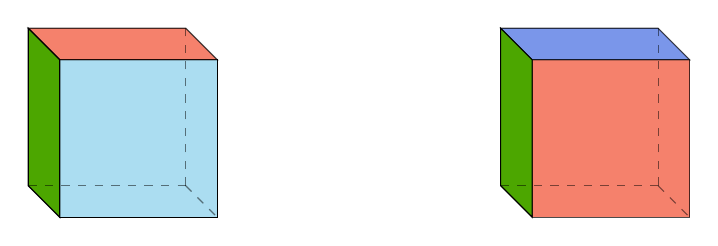
\begin{tikzpicture}[scale=1, line width=0.4pt]
        % 左正方体
        \coordinate (F_BL) at (2.2,0);
        \coordinate (F_BR) at (4.2,0);
        \coordinate (F_TR) at (4.2,2);
        \coordinate (F_TL) at (2.2,2);

        \coordinate (B_BL) at (1.8,0.4);
        \coordinate (B_TL) at (1.8,2.4);
        \coordinate (B_TR) at (3.8,2.4);
        \coordinate (B_BR) at (3.8,0.4);

        \filldraw[fill=SkyBlue!70!white, draw=black] (F_BL) -- (F_BR) -- (F_TR) -- (F_TL) -- cycle;
        \filldraw[fill=RedOrange, opacity=0.7, draw=black] (F_TL) -- (F_TR) -- (B_TR) -- (B_TL) -- cycle;
        \filldraw[fill=Green!70!yellow, draw=black] (F_BL) -- (F_TL) -- (B_TL) -- (B_BL) -- cycle;
        % 隐藏边虚线
        \draw[opacity=0.5, dashed] (B_BL) -- (B_BR);
        \draw[opacity=0.5, dashed] (B_BR) -- (F_BR);
        \draw[opacity=0.5, dashed] (B_BR) -- (B_TR);

        % 右正方体
        \begin{scope}[xshift=6cm]
            \coordinate (F_BL) at (2.2,0);
            \coordinate (F_BR) at (4.2,0);
            \coordinate (F_TR) at (4.2,2);
            \coordinate (F_TL) at (2.2,2);

            \coordinate (B_BL) at (1.8,0.4);
            \coordinate (B_TL) at (1.8,2.4);
            \coordinate (B_TR) at (3.8,2.4);
            \coordinate (B_BR) at (3.8,0.4);

            \filldraw[fill=RedOrange, opacity=0.7, draw=black] (F_BL) -- (F_BR) -- (F_TR) -- (F_TL) -- cycle;
            \filldraw[fill=RoyalBlue, opacity=0.7, draw=black] (F_TL) -- (F_TR) -- (B_TR) -- (B_TL) -- cycle;
            \filldraw[fill=Green!70!yellow, draw=black] (F_BL) -- (F_TL) -- (B_TL) -- (B_BL) -- cycle;
            % 隐藏边虚线
            \draw[opacity=0.5, dashed] (B_BL) -- (B_BR);
            \draw[opacity=0.5, dashed] (B_BR) -- (F_BR);
            \draw[opacity=0.5, dashed] (B_BR) -- (B_TR);
        \end{scope}
    \end{tikzpicture}
    \label{fig:example-cube-1}
\end{figure}
\vspace{16pt}

不过，也可以说它先朝左转动了$90^\circ$，让上面（浅红色）变成左面，保持前后面（蓝色）不变；然后再往右转了$90^\circ$，让左面（浅红色）变成前面，保持上下面（绿色）不变；再往右转动了$90^\circ$，让上面（浅绿色）变成右面，保持前后面（红色）不变。

\vspace{16pt}
\begin{figure}[htbp]
    \centering
    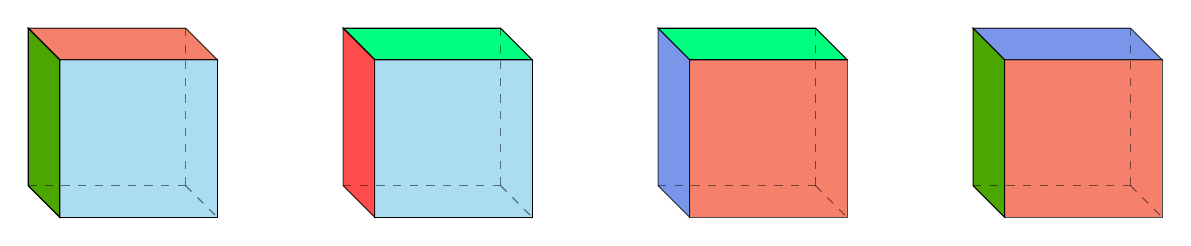
\begin{tikzpicture}[scale=1, line width=0.4pt]
        % 左正方体
        \coordinate (F_BL) at (2.2,0);
        \coordinate (F_BR) at (4.2,0);
        \coordinate (F_TR) at (4.2,2);
        \coordinate (F_TL) at (2.2,2);

        \coordinate (B_BL) at (1.8,0.4);
        \coordinate (B_TL) at (1.8,2.4);
        \coordinate (B_TR) at (3.8,2.4);
        \coordinate (B_BR) at (3.8,0.4);

        \filldraw[fill=SkyBlue!70!white, draw=black] (F_BL) -- (F_BR) -- (F_TR) -- (F_TL) -- cycle;
        \filldraw[fill=RedOrange, opacity=0.7, draw=black] (F_TL) -- (F_TR) -- (B_TR) -- (B_TL) -- cycle;
        \filldraw[fill=Green!70!yellow, draw=black] (F_BL) -- (F_TL) -- (B_TL) -- (B_BL) -- cycle;
        % 隐藏边虚线
        \draw[opacity=0.5, dashed] (B_BL) -- (B_BR);
        \draw[opacity=0.5, dashed] (B_BR) -- (F_BR);
        \draw[opacity=0.5, dashed] (B_BR) -- (B_TR);

        % 中正方体
        \begin{scope}[xshift=4cm]
            \coordinate (F_BL) at (2.2,0);
            \coordinate (F_BR) at (4.2,0);
            \coordinate (F_TR) at (4.2,2);
            \coordinate (F_TL) at (2.2,2);

            \coordinate (B_BL) at (1.8,0.4);
            \coordinate (B_TL) at (1.8,2.4);
            \coordinate (B_TR) at (3.8,2.4);
            \coordinate (B_BR) at (3.8,0.4);

            \filldraw[fill=SkyBlue!70!white, draw=black] (F_BL) -- (F_BR) -- (F_TR) -- (F_TL) -- cycle;
            \filldraw[fill=SpringGreen, draw=black] (F_TL) -- (F_TR) -- (B_TR) -- (B_TL) -- cycle;
            \filldraw[fill=Red!, opacity=0.7, draw=black] (F_BL) -- (F_TL) -- (B_TL) -- (B_BL) -- cycle;
            % 隐藏边虚线
            \draw[opacity=0.5, dashed] (B_BL) -- (B_BR);
            \draw[opacity=0.5, dashed] (B_BR) -- (F_BR);
            \draw[opacity=0.5, dashed] (B_BR) -- (B_TR);
        \end{scope}

        % 右正方体
        \begin{scope}[xshift=8cm]
            \coordinate (F_BL) at (2.2,0);
            \coordinate (F_BR) at (4.2,0);
            \coordinate (F_TR) at (4.2,2);
            \coordinate (F_TL) at (2.2,2);

            \coordinate (B_BL) at (1.8,0.4);
            \coordinate (B_TL) at (1.8,2.4);
            \coordinate (B_TR) at (3.8,2.4);
            \coordinate (B_BR) at (3.8,0.4);

            \filldraw[fill=RedOrange, opacity=0.7, draw=black] (F_BL) -- (F_BR) -- (F_TR) -- (F_TL) -- cycle;
            \filldraw[fill=SpringGreen, draw=black] (F_TL) -- (F_TR) -- (B_TR) -- (B_TL) -- cycle;
            \filldraw[fill=RoyalBlue, opacity=0.7, draw=black] (F_BL) -- (F_TL) -- (B_TL) -- (B_BL) -- cycle;
            % 隐藏边虚线
            \draw[opacity=0.5, dashed] (B_BL) -- (B_BR);
            \draw[opacity=0.5, dashed] (B_BR) -- (F_BR);
            \draw[opacity=0.5, dashed] (B_BR) -- (B_TR);
        \end{scope}
        % 右正方体
        \begin{scope}[xshift=12cm]
            \coordinate (F_BL) at (2.2,0);
            \coordinate (F_BR) at (4.2,0);
            \coordinate (F_TR) at (4.2,2);
            \coordinate (F_TL) at (2.2,2);

            \coordinate (B_BL) at (1.8,0.4);
            \coordinate (B_TL) at (1.8,2.4);
            \coordinate (B_TR) at (3.8,2.4);
            \coordinate (B_BR) at (3.8,0.4);

            \filldraw[fill=RedOrange, opacity=0.7, draw=black] (F_BL) -- (F_BR) -- (F_TR) -- (F_TL) -- cycle;
            \filldraw[fill=RoyalBlue,opacity=0.7, draw=black] (F_TL) -- (F_TR) -- (B_TR) -- (B_TL) -- cycle;
            \filldraw[fill=Green!70!yellow, draw=black] (F_BL) -- (F_TL) -- (B_TL) -- (B_BL) -- cycle;
            % 隐藏边虚线
            \draw[opacity=0.5, dashed] (B_BL) -- (B_BR);
            \draw[opacity=0.5, dashed] (B_BR) -- (F_BR);
            \draw[opacity=0.5, dashed] (B_BR) -- (B_TR);
        \end{scope}
    \end{tikzpicture}
    \label{fig:example-cube-2}
\end{figure}
\vspace{16pt}

如果这个方块不是正方体，而是长方体呢？那么不需要通过颜色分辨，你就能看出它动过了。因为朝前转动$90^\circ$会让它的形状看起来不一样。

这种区别的背后，是什么在起作用呢？

再想象一个正三角形。按它的中心，逆时针旋转，你会发现，旋转$120^\circ$后，看起来和原来一样。顺时针旋转$120^\circ$也是如此。要区别这些状态，可以给三角形的顶点按逆时针方向依次标上颜色，比如红色、绿色、蓝色。你会发现，前一个旋转把红色顶点转到了绿色顶点的位置，把绿色顶点转到了蓝色顶点的位置，把蓝色顶点转到了红色顶点的位置。后一个旋转则把红色顶点转到了蓝色顶点的位置，把蓝色顶点转到了绿色顶点的位置，把绿色顶点转到了红色顶点的位置。这下我们能清楚区分这两个旋转了。

\vspace{12pt}
\begin{figure}[htbp]
    \centering
    \begin{tikzpicture}[>=Stealth, scale=1.2, thick]
  % 定义三个三角形的中心高度（等边三角形边长=2，高=sqrt(3)）
  \def\height{1.732}
  \def\halfwidth{1}
  \def\topper{1}
  \def\psiz{4pt}
  
  % ========== 1. 左侧：初始状态（恒等变换 e） ==========
  \begin{scope}[shift={(0,0)}]
    \coordinate (A1) at (0,0);          % 左下
    \coordinate (B1) at (2,0);          % 右下
    \coordinate (C1) at (1,\height);    % 上顶点
    
    \draw (A1) -- (B1) -- (C1) -- cycle;
    \fill[LimeGreen] (A1) circle (\psiz) node[left=4pt,color=Green!50!black] {};
    \fill[RoyalBlue] (B1) circle (\psiz) node[right=4pt,color=Blue] {};
    \fill[BrickRed] (C1) circle (\psiz) node[above=4pt,color=BrickRed!50!black] {};
    % \node at (1, \height/3) {$e$}; % 中心标注单位元
  \end{scope}

  % ========== 2. 中间：逆时针旋转 120° ==========
  \begin{scope}[shift={(4,0)}]
    \coordinate (A2) at (0,0);
    \coordinate (B2) at (2,0);
    \coordinate (C2) at (1,\height);
    
    \draw (A2) -- (B2) -- (C2) -- cycle;
    \fill[LimeGreen] (B2) circle (\psiz) node[right=4pt,color=Green!50!black] {};
    \fill[RoyalBlue] (C2) circle (\psiz) node[above=4pt,color=Blue] {};
    \fill[BrickRed] (A2) circle (\psiz) node[left=4pt,color=BrickRed!50!black] {};
    % \node at (1, \height/3) {$r$};
  \end{scope}

  % ========== 3. 右侧：顺时针旋转 120° ==========
  \begin{scope}[shift={(8,0)}]
    \coordinate (A3) at (0,0);
    \coordinate (B3) at (2,0);
    \coordinate (C3) at (1,\height);
    
    \draw (A3) -- (B3) -- (C3) -- cycle;
    \fill[LimeGreen] (C3) circle (\psiz) node[above=4pt,color=Green!50!black] {};
    \fill[RoyalBlue] (A3) circle (\psiz) node[left=4pt,color=Blue] {};
    \fill[BrickRed] (B3) circle (\psiz) node[right=4pt,color=BrickRed!50!black] {};
    % \node at (1, \height/3) {$r^2$};
  \end{scope}

  % ========== 4. 绘制带方向箭头的 120° 弧线 ==========
  \def\radius{0.8}
  
  % 中间：逆时针弧线
  \draw[->, >=Stealth] 
    (5, \height/3 + \topper) ++(30:\radius) arc (30:150:\radius);
  \node[above] at (5, \height/3 + \topper + \radius) {逆时针$120^\circ$};

  % 右侧：顺时针弧线
  \draw[->, >=Stealth] 
    (9, \height/3 + \topper) ++(150:\radius) arc (150:30:\radius);
  \node[above] at (9, \height/3 + \topper + \radius) {顺时针$120^\circ$};

    \end{tikzpicture}
    \label{fig:example-triangle-1}
\end{figure}
\vspace{12pt}

此外，如果把正三角形沿某条中线翻转，它看起来也不变。可要是我们把顶点标上颜色，就能看到变化了。

\vspace{12pt}
\begin{figure}[htbp]
    \centering
    \begin{tikzpicture}[>=Stealth, scale=1.2, thick]
    \def\height{1.732}  % 三角形高
    \def\shiftx{4}    % 三角形之间的水平间距
    \def\radius{0.35}  % 翻转箭头的圆弧半径
    \def\axismore{0.5}  % 翻转轴虚线超出三角形的部分
    \def\psiz{4pt}

    % ========== 翻转①：沿顶点1到对边的中线 ==========
    \begin{scope}[shift={(0,0)}]
        % 三角形顶点（相对坐标）
        \coordinate (BL) at (0,0);
        \coordinate (BR) at (2,0);
        \coordinate (T)  at (1,\height);
        \coordinate (C) at (1,\height/3);
        
        % 翻转轴（虚线中线）
        \draw[dashed, thick, gray] ($(C)!1.5!(T)$) -- ($(T)!2!(C)$);
        \draw (BL) -- (BR) -- (T) -- cycle;
        
        % 标记（翻转后标签：上=1，左下=3，右下=2）
        \fill[LimeGreen] (BR) circle (\psiz) node[right=4pt, color=Green!50!black] {};
        \fill[RoyalBlue] (BL) circle (\psiz) node[left=4pt,  color=Blue] {};
        \fill[BrickRed]  (T)  circle (\psiz) node[above=4pt, color=BrickRed!50!black] {};
        
        % 翻转箭头（底边下方，半圆弧）
        \draw[->, thick] (C) ++ (-90:\radius) ++ (180:\radius) arc (180:0:\radius);  % 从左侧到右侧，向下凸
    \end{scope}

    % ========== 翻转②：沿顶点2到对边的中线 ==========
    \begin{scope}[shift={(\shiftx,0)}]
        \coordinate (BL) at (0,0);
        \coordinate (BR) at (2,0);
        \coordinate (T)  at (1,\height);
        \coordinate (C) at (1,\height/3);
        
        % 翻转轴：从BL到对边（右斜边）中点
        \draw[dashed, thick, gray] ($(C)!1.5!(BL)$) -- ($(BL)!2!(C)$);
        \draw (BL) -- (BR) -- (T) -- cycle;
        
        % 翻转后标签：上=3，左下=2，右下=1
        \fill[LimeGreen] (BL) circle (\psiz) node[left=4pt,  color=Green!50!black] {};
        \fill[RoyalBlue] (T)  circle (\psiz) node[above=4pt, color=Blue] {};
        \fill[BrickRed]  (BR) circle (\psiz) node[right=4pt, color=BrickRed!50!black] {};
        
        \draw[->, thick] (C) ++ (30:\radius) ++ (-60:\radius) arc (300:120:\radius);
    \end{scope}

    % ========== 翻转③：沿顶点3到对边的中线 ==========
    \begin{scope}[shift={(2*\shiftx,0)}]
        \coordinate (BL) at (0,0);
        \coordinate (BR) at (2,0);
        \coordinate (T)  at (1,\height);
        \coordinate (C) at (1,\height/3);
        
        % 翻转轴：从BR到对边（左斜边）中点
        \draw[dashed, thick, gray]  ($(C)!1.5!(BR)$) -- ($(BR)!2!(C)$);
        \draw (BL) -- (BR) -- (T) -- cycle;
        
        % 翻转后标签：上=2，左下=1，右下=3
        \fill[LimeGreen] (T)  circle (\psiz) node[above=4pt, color=Green!50!black] {};
        \fill[RoyalBlue] (BR) circle (\psiz) node[right=4pt,  color=Blue] {};
        \fill[BrickRed]  (BL) circle (\psiz) node[left=4pt, color=BrickRed!50!black] {};
        
        \draw[->, thick] (C) ++ (150:\radius) ++ (-120:\radius) arc (-120:60:\radius);
    \end{scope}

    \end{tikzpicture}
    \label{fig:example-triangle-2}
\end{figure}
\vspace{12pt}

而要是三角形不是正三角形，比如三边都不一样长，那么除非旋转一周，否则不会看起来和原来一样。旋转$120^\circ$和沿中线翻转都没用了。

正方体、正三角形都有某种性质，在某些变换下不变，我们称其为\textbf{对称性}。日常语言中的对称是指左右手、左右眼这样的关系，也就是按轴线或平面翻转后不变。数学里，我们把“在某些变换下不变”的性质都称为对称性。我们已经讨论过的对称性有平面形的轴对称和中心对称。前面的例子里翻面或旋转不变也是一种对称。对称能帮助我们思考。比如，我们说偶函数的图像关于$y$轴对称，所以只要理解了函数在$x>0$时的性质，就能让我们理解它在$x<0$时的性质。不过，对于对称本身，我们还没有展开研究。具体来说，造成对称的是某种抽象规律，而数学就是抽离表象、揭示内在规律的学科。下面就让我们来研究对称背后的道理。

\section{变换的规则}

为什么正方体和正三角形通过翻转、旋转看起来不变？因为它们所有的边都一样长，所有的角都一样大，所有的面都一样。这种对称性导致它们在某些变换下不变。反过来说，这些变换刻画了它们的对称性质。通过研究这些变换，我们就能理解对称。

前面的例子里，我们给正三角形的顶点标记了颜色。我们发现，顺时针、逆时针旋转$120^\circ$，改变了顶点的颜色。通过这个做法，我们发现有$6$种变换能让正三角形看起来不变。分别是顺时针、逆时针旋转$120^\circ$，沿$3$条中线翻转，以及什么也不做（没错，我们把这种“变换”也考虑在内）。这就是我们感兴趣的所有变换。

正方体的情形则更复杂。它有$6$个面。首先可以把任一个面转到朝上；接着，不改变朝上的面，可以把$4$个侧面之一转到正对我们。因此，一共有$6\times 4 = 24$种转动方法。这就是我们感兴趣的所有变换。

一旦确立了要研究的变换的集合，我们就不再改动了。这个集合就是我们研究的“舞台”。

接着，我们来考察各种变换的关系。

首先，我们只考虑理想的变换。比如某次旋转三角形的时候角度差了一点点，某次转动方块的时候整体位置稍微动了一点，这种问题我们不考虑在内。我们讨论的是抽象的理想的情况。同一个变换每次操作的效果是一致的，每个变换的效果是确定的。

其次，每个变换都是可逆的，逆变换也在集合里。比如，我们有把正三角形沿逆时针旋转$120^\circ$的变换，就有把正三角形沿顺时针旋转$120^\circ$的变换。它恢复“逆时针旋转$120^\circ$”这个操作。正方体的变换里，每种方式转过后，也可以逆着转回来。

最后，变换的组合还是某种变换。比如我们会发现：把正三角形沿逆时针旋转$120^\circ$两次，效果和沿顺时针针旋转$120^\circ$是一样的。把正方体顶面转到左面、右转$90^\circ$、再把顶面转到右侧面，效果和把顶面转到正面是一样的。无论怎么变，结果总是集合里的某种变换。

我们来总结一下这些规则：
\begin{enumerate}[label=\arabic*.]
    \item 有一个确定不变的、由变换构成的集合。
    \item 每个变换的效果是确定的。
    \item 每个变换的效果是可逆的。
    \item 变换的组合还是某种变换。
\end{enumerate}
这就是我们从正三角形和正方体的例子里抽离出来的规则。它们似乎已经足够多了。
现在就让我们来研究根据这些规则得到的系统。我们把它称为\textbf{群}，看看它有什么性质。

\section{群有哪些？}

首先你可能想要知道，除了正三角形和正方体，还有哪些东西符合这个群的定义。我们大致能想象到正四边形（正方形）、正五边形里大概也有相关的群。不过，更聪明的读者也许会联想到更远的地方。比如，几个人坐在圆桌边上，不同的坐法之间有什么关联呢？我们可以把每种调换位子的方法看作一种变换。所有的变换构成一个集合；每种变换的效果是确定的；调换位子后肯定能调换回来；最后，几个调换位子的方法组合起来，必然也是一种调换位子的方法。所以，不同的坐法背后也是一个群。

又比如，我们玩扑克牌之前也许会洗牌，把牌打乱。每次洗牌都是变换牌的顺序。所有变换扑克牌顺序的方法构成确定的集合；每种方法的结果是确定的；每次洗牌的效果是可逆的（也许经过魔术师的训练才能做到，但我们不难想象理想情况下的效果）；最后，无论洗多少次牌，效果也是变换扑克牌的顺序，还是某种变换。所以，扑克牌的所有可能的洗牌变换也是一个群。

我们还可以考虑数学里的场景。比如，考虑模$5$的同余类，我们知道它可以写成：
$$ \left\{\overline{0},\,\overline{1},\,\overline{2},\,\overline{3},\,\overline{4}\right\} $$
从某个数（比如$0$）出发，通过加法，我们把它变成属于其他的同余类。比如“加$1$”变换就把$0$从同余类$\overline{0}$的成员，变成$\overline{1}$的成员。这样的变换一共$5$种，构成确定的集合；每个变换的效果是确定的。不仅如此，变换的组合仍然是变换。比如“加$1$”然后“加$2$”的效果就是“加$3$”。最后，变换的效果是可逆的，比如加$1$之后再加$4$，就能把一个数变回原来的同余类；加$3$之后要变回原来的同余类，只需再加$2$。等等。可以验证每个变换都可逆。于是，模$n$同余类通过加法也定义了一个群，记为$\mathbb{Z}_n$。

群的元素个数可以是无限的。比如，对于圆来说，所有绕圆心的旋转构成群。这样的旋转有无限个。我们沿用集合的称呼，把群的大小称为群的\textbf{势}。对于有限个变换构成的群，变换的个数就是群的势。无限个变换构成的群，它的势要和我们常见的无限集合比较，这里不多叙述。

上面的说法，让我们觉得群似乎无处不在。然而，也有些结构并不是群。比如，把以上的模$5$同余类换成自然数集$\mathbb{N}$，考虑“加$1$”、“加$2$”等变换，它们确实也构成确定的集合，效果也是确定的，甚至若干个“加几”变换组合起来，还是某种“加几”变换。唯一的问题是：“加几”变换不是可逆的。我们没法通过“加几”把“加$1$”的效果逆转。所以“加几”定义的变换集合不是群。不过，如果我们把范围扩大到整数集$\mathbb{Z}$，就会发现，“加几”又构成群了。因为这时候，“加$-1$”就是减$1$，能逆转“加$1$”的效果了。

我们可以画一个数轴来理解这件事。数轴上，“加几”就是从原点出发往右移到某个整点。如果只考虑自然数，那么只有右半边的数轴。如果考虑全体整数，则变成既可以往左移动，也可以往右移动，这就覆盖了整个数轴，左右对称了。所以群必然体现了某种对称性。不构成群，往往意味着某个方面还不够对称。

\begin{et}
    以下的例子里是否包含群？
    \begin{enumerate}[label=\arabic*).]
        \item 一枚金币和一枚银币放在桌子上，都分正反面。每次可以选择翻动一枚币。这样的变换有几个？是否构成了群？
        \item 同上情况。每次可以选择翻动一枚币、两枚币，或者什么都不做。这样的变换有几个？是否构成了群？
        \item 同上情况。每次要么同时翻动两枚币，要么什么都不做。这样的变换有几个？是否构成了群？
        \item 考虑集合$A$到$B$的映射，这些映射是否构成了群？
        \item 考虑集合到自身的所有映射，这些映射是否构成了群？
        \item 考虑集合到自身的所有双射，这些双射是否构成了群？
    \end{enumerate}
\end{et}

\begin{so}
     \mbox{} \\
     \indent 1). 每次恰好翻动一枚币，所以变换只有$2$个：翻金币、翻银币。
     翻金币后再翻银币，两枚币都翻面，可是“同时翻两枚”并不在这$2$个变换之中。
     按规定，两个变换的组合无法用一次变换实现，不在集合里，不满足规则$4$。
     因此不构成群。

     2). 变换有$4$个：什么都不做、只翻金币、只翻银币、同时翻两枚。
     规则$1$、$2$显然成立。
     每个变换做两次都恢复原状，因此满足规则$3$。
     再验证规则$4$：任取两个不同的变换连续做，效果仍然是这$4$个变换之一。
     比如“只翻金币”接着“只翻银币”，效果等于“同时翻两枚”；
     “只翻金币”接着“同时翻两枚”，效果等于“只翻银币”。
     其他组合也可以逐一验证。这说明任意两种变换连续做的结果是某一个变换。于是对于多于两个变换的组合，可以不断把前两个变换替换成一个，最终简化成一个变换。于是规则$4$满足。
     综上可知构成群。

     3). 变换有$2$个：什么都不做、同时翻两枚。
     规则$1$、$2$显然成立。
     “同时翻两枚”做两次，两枚币都翻了两次，恢复原状，
     效果等于“什么都不做”。所以它的逆变换就是它自己，满足规则$3$。
     再验证规则$4$：两个变换的任意组合仍在集合中。比如“同时翻两枚”接“同时翻两枚”等于“什么都不做”，
     其余组合更不成问题。同前一题可知规则$4$满足。
     综上可知构成群。

     4). 集合$A$到集合$B$的映射，不一定能两两复合：
     第一个映射把$A$中的元素映射到$B$中，
     第二个映射也要从$A$出发，可是它的输入是$B$中的元素。
     除非$B = A$，否则复合没有定义，规则$4$无从谈起。
     即使$B = A$，一般的映射也未必可逆（比如把$A$中所有元素都映到同一个元素的常映射，就无法从结果还原输入），规则$3$也不满足。因此不构成群。

     5). 集合到自身的映射，复合之后仍是集合到自身的映射，
     满足规则$4$。每个映射的效果是确定的，满足规则$2$。
     但并非每个映射都可逆。
     比如集合$\{1,2\}$到自身的映射“把$1$和$2$都映到$1$”，
     无论再做任何映射，都不可能把$1$还原为原来的$1$和$2$两个不同的元素。
     所以规则$3$不满足。
     因此不构成群。

     6). 集合到自身的双射，就是一一对应的映射。
     规则$1$、$2$显然成立。
     每个双射都可逆，且逆映射也是双射，满足规则$3$。
     两个双射复合仍是双射，满足规则$4$。
     因此构成群。
\end{so}

\clearpage

\section*{本章小结}

本章我们从正三角形和正方体的对称变换出发，抽离出了对称现象背后的规则。一个群就是一个由“变换”构成的系统，它必须满足四个基本条件：
\begin{itemize}
    \item \textbf{集合确定}：变换的集合是明确且固定的。
    \item \textbf{效果确定}：每个变换的效果是确定的，这保证了运算的结合律。
    \item \textbf{操作可逆}：每个变换都存在逆变换，能够撤销其效果。
    \item \textbf{组合封闭}：任意两个变换的组合（复合）仍然是该集合中的变换。
\end{itemize}
通过圆桌座位、洗牌等例子，我们看到群广泛存在于各种具有对称性的场景中。群是描述和研究对称性的语言。群的大小（元素个数）称为群的势。

\clearpage

\section{练习}

以下习题是帮助你理解刚刚讨论的概念的思想实验。在数学及类似的科学工作中，习题通常需要一些思考，会让你花费一些时间。本书并不会要求你反复琢磨每一段文字，大可以快速浏览内容，欣赏大略的思想。不过对于较为抽象的概念，只有经过一番思考，才能真正深入地理解其机理。因此，在习题上花费一些时间很正常，不要气馁。

同样，在习题上花费过多的时间，也是没必要的。到附录里查看习题的答案或解题思路，也不必感到不好意思。习题并不是为了刁难人而设置的。因此，思考几分钟无果，就查看答案来掌握思考方法，也是合理的策略。像读小说一样，完全不看习题，直接阅读下一章，也没有问题。

\subsection*{是不是群}

\begin{problemlist}
  \item 将一枚金币和一枚银币放在桌子上。考虑一个动作：交换两枚硬币的位置。这是群吗？
  \item 在上述两币旁再放一个金币。仍然只考虑交换前两枚钱币的位置。这是群吗？
  \item 你左边的裤袋子里有$5$个弹珠，右边的裤带子里也有$5$个弹珠。考虑两种动作：从左裤袋里拿一个弹珠放到右边裤袋里；以及从右裤袋里拿一个弹珠放到左边裤袋里。这是群吗？
  \item 画廊的一间陈列室里有四面墙，其中三面墙上各挂着一幅画，每面墙上一幅。经理想重新排列这三幅画。每面墙只能挂一幅画，靠出口大门的墙不能挂画。
  \begin{problemlist}
    \item 一共有几种挂画方法？
    \item 如果只允许两种重排方法：交换左墙和中间墙上的画，或者交换左墙和右墙上的画。只通过这两种手段，能实现任意的挂画方法吗？
    \item 这两种重排方法是群吗？如果不是，还差了什么？
    \item 如果靠出口大门的墙也能挂画了，情况会如何变化？以上问题的答案会变吗？
  \end{problemlist}
\end{problemlist}

\subsection*{谈谈规则}

\begin{problemlist}
    \item 一个群里的变换是否一定有限？是否一定能列举出来？
    \item 如果分析某个对象的对称性，发现只有“什么都不做”这个变换满足条件，这表示对象的对称性有什么特征？
    \item 对以下每个要求，构造一个额外满足此要求的群。
    \begin{problemlist}
        \item 变换组合的顺序会影响最终的效果。
        \item 变换组合的顺序不影响最终的效果。
        \item 恰好包含两个变换。
        \item 恰好包含三个变换。
        \item 恰好包含四个变换。
    \end{problemlist}
    \item 任给一个正整数$n$，你能构造一个恰包含$n$个变换的群吗？你能让这个群里出现“变换组合的顺序影响最终效果”的情况吗？
\end{problemlist}

\subsection*{打破规则}

下面来谈谈我们给群定的规则是否是必须的。不遵守这些规则会出现什么情况。第一条规则是基础的，离开它我们甚至不能确定我们在讨论什么东西。所以下面只讨论第二、三、四条规则，想想没了这些规则会得到什么。
\begin{problemlist}
    \item 仿照以下例子，设计一个仅仅不满足第二条规则的情形。例子：考虑一块可擦除的电子白板。变换是“在白板上写点东西”。每次写的内容是不确定的，所以不满足第二条规则。但其他规则都符合。
    \item 仿照以下例子，设计一个仅仅不满足第三条规则的情形。例子：考虑无限多的火柴，变换是“抽出一根火柴划着”。由于火柴划着后就无法复原了，所以效果不可逆，不满足第三条规则。但其他规则都符合。
    \item 仿照以下例子，设计一个仅仅不满足第四条规则的情形。例子：考虑所有整数，变换是“加$1$”和“减$1$”。由于“加$1$”重复两次就不再是“加$1$”、“减$1$”之一，所以不满足第四条规则。但其他规则都符合。
\end{problemlist}

\subsection*{数与群}

群和数有天然的联系。因此，讨论数中的群也是理所当然。

\begin{problemlist}
    \item 考虑前面整数集$\mathbb{Z}$例子里的“加几”群。如果把“加几”的“几”限定为偶数，还构成群吗？
    \item 同样，如果限定为奇数，还构成群吗？
    \item 同样，如果限定为$3$的倍数，还构成群吗？如果限制成模$3$余$1$的数呢？
    \item 如果把“加几”改为“乘几”，构成群吗？
    \item 如果把$\mathbb{Z}$改为非零整数集，那么所有“乘几”构成群吗？
    \item 如果把$\mathbb{Z}$改为非零有理数集，那么所有“乘几”构成群吗（这里的“几”可以是任何非零的有理数）？
    \item 考虑正整数$n$的同余类：$\overline{0},\overline{1},\cdots,\overline{n-1}$。把“乘几”定义为同余类的乘法，那么所有“乘几”构成群吗？如果只考虑非零同余类呢？
    \item 考虑素数$p$的非零同余类：$\overline{1},\cdots,\overline{p-1}$。设$\overline{a}$是其中一个同余类。如果从$\overline{a}$开始，不断重复乘$\overline{a}$，能构成所有的非零同余类，就说$a$是模$p$的原根。哪些$a$是原根，哪些不是？对$p=3,5,7,11$分别查找原根。
\end{problemlist}

\chapter{群是什么样子的？}

\vspace{-24pt}
\begin{figure}[htbp]
    \centering
    \includegraphics[width=\textwidth]{tu/三垣四象二十八宿.jpg}
    \label{fig:example-nightsky-constellation-ancient-china}
\end{figure}

\section{连线图}

上一章我们引入了“群”的概念，还举出了不少例子。不过，单单用文字来描述群的性质，总仿佛隔着一层薄纱，朦朦胧胧看不清楚。一个群里有多少个变换？这些变换之间是什么关系呢？用文字来描述，反而更让人困惑了。这是因为对称和变换本身就是抽象的概念。我们需要找到把它们看清楚的方法。

正三角形和正方体的例子里，我们试图用图像来理解群，不过做得还不够。正三角形相关的群就有$6$个变换，而正方体相关的群有$24$个变换。我们小时候玩过的魔方，虽然也是正方体，通过把每个面扭转到不同的方向，竟然能够变出$4$千亿亿种不同的状态。这样繁多的变换，犹如漫天星辰，如何去理解？

古人观天时，想要找到一颗星星，怎么做呢？他们把位置相近的星星在头脑里连起来，想象成互相关联的一个整体。这样，只要找到了最亮的那颗星，就能跟着头脑里的连线，找到其他的星星了。这启发我们用连线的方式来表示变换。我们可以把不同的状态看作“星星”，把状态之间的变换用连线来表示。和天上的星星相比，我们的优势是能够任意排布这些“星星”的位置，方便我们连线。

首先来看正三角形的例子。上一章里我们列举了$6$个变换。这些变换之间有什么联系呢？我们从正三角形的某个状态出发，把它称为初始状态，记为$A_1$，然后看它经历不同的变换变成什么样子。

\begin{figure}[htbp]
    \centering
    \begin{tikzpicture}[>=Stealth, thick, font=\normalsize]
        
        % 设定边界，防止右侧文字被裁剪
        \path (6.5, -3.5) rectangle (-4, 3.5); 

        % ================= 左侧主图 =================
        
        % 1. 绘制中心“初始状态”
        % 实例化名称为 C0，颜色排布：上红, 左下绿, 右下蓝
        \pic (C0) at (0,0) {tri={BrickRed}{LimeGreen}{RoyalBlue}};
        % 【关键修复】：使用 C0-C 来引用 pic 内部定义的中心坐标
        \node at (C0-C) {$A_1$};

        % 2. 绘制周围六边形排布的 6 个状态
        \def\R{2.25}      % 六边形半径 (已减半)
        \def\rscale{0.8} % 周围三角形的缩放比例
        
        % A1 (正上方, 90度) - 恒等变换 e
        \pic[scale=\rscale] (A1) at (90:\R) {tri={BrickRed}{LimeGreen}{RoyalBlue}};
        \node at (A1-C) {$A_1$};

        % A2 (右上, 30度) - 逆时针旋转120度 r1
        \pic[scale=\rscale] (A2) at (30:\R) {tri={RoyalBlue}{BrickRed}{LimeGreen}};
        \node at (A2-C) {$A_2$};

        % A3 (右下, -30度) - 顺时针旋转120度 r2
        \pic[scale=\rscale] (A3) at (150:\R) {tri={LimeGreen}{RoyalBlue}{BrickRed}};
        \node at (A3-C) {$A_3$};

        % A4 (正下方, -90度) - 竖直翻转 s1
        \pic[scale=\rscale] (A4) at (-90:\R) {tri={BrickRed}{RoyalBlue}{LimeGreen}};
        \node at (A4-C) {$A_4$};

        % A5 (左下, -150度) - 左下-右上翻转 s2
        \pic[scale=\rscale] (A5) at (-150:\R) {tri={RoyalBlue}{LimeGreen}{BrickRed}};
        \node at (A5-C) {$A_5$};

        % A6 (左上, 150度) - 右下-左上翻转 s3
        \pic[scale=\rscale] (A6) at (-30:\R) {tri={LimeGreen}{BrickRed}{RoyalBlue}};
        \node at (A6-C) {$A_6$};

        % 3. 绘制从中心发散的 6 个箭头及中部标签
        \draw[->, gray!70] ($(0,0)!1.0cm!(90:\R)$) -- ($(90:\R)!0.4cm!(0,0)$)  
            node[pos=0.5, right=0pt, color=black] {$e$};
            
        \draw[->, gray!70] ($(0,0)!0.5cm!(30:\R)$) -- ($(30:\R)!0.8cm!(0,0)$)
            node[pos=0.4, above=1pt, color=black] {$r_1$};
            
        \draw[->, gray!70] ($(0,0)!1.0cm!(-30:\R)$) -- ($(-30:\R)!0.4cm!(0,0)$)
            node[pos=0.5, above=1pt, color=black] {$s_3$};
            
        \draw[->, gray!70] ($(0,0)!0.5cm!(-90:\R)$) -- ($(-90:\R)!0.8cm!(0,0)$)  
            node[pos=0.5, left=-1pt, color=black] {$s_1$};
            
        \draw[->, gray!70] ($(0,0)!1.0cm!(-150:\R)$) -- ($(-150:\R)!0.4cm!(0,0)$)
            node[pos=0.5, above=1pt, color=black] {$s_2$};
            
        \draw[->, gray!70] ($(0,0)!0.5cm!(150:\R)$) -- ($(150:\R)!0.8cm!(0,0)$)
            node[pos=0.4, above=1pt, color=black] {$r_2$};

        % ================= 右侧纯动作符号说明 =================
        
        % 定义单元格坐标 (3行2列布局)
        \def\colL{7.0}   % 左列中心 x (向右平移，避免与主图重叠)
        \def\colR{10.0}   % 右列中心 x (间距调整为 2.8，约为原来的 80%)
        \def\rowI{2.3}   % 第一行 y
        \def\rowII{0.0}  % 第二行 y
        \def\rowIII{-2.3}% 第三行 y
        \def\hgap{1}

        % --- 第一行： e | s_1 ---
        % e (恒等变换：虚线空白大方框，大小调整为 1.28x1.28)
        \node at (\colL - \hgap, \rowI) {$e$}; % 字母向左移，避免与图示重叠
        \begin{scope}[shift={(\colL, \rowI)}]
            \draw[dashed, thick, gray] (-0.64, -0.64) rectangle (0.64, 0.64);
        \end{scope}
        
        % s_1 (竖直翻转：轴长 1.6，弧半径 0.48)
        \node at (\colR - \hgap, \rowI) {$s_1$};
        \begin{scope}[shift={(\colR, \rowI)}]
            \draw[dashed, thick, gray] (0, -0.8) -- (0, 0.8);
            \draw[->, thick] (-0.48, -0.48) arc (180:0:0.48);
        \end{scope}

        % --- 第二行： r_1 | s_2 ---
        % r_1 (逆时针旋转：弧半径 0.64)
        \node at (\colL - \hgap, \rowII) {$r_1$};
        \begin{scope}[shift={(\colL, \rowII)}]
            \draw[->, thick] (30:0.64) arc (30:150:0.64);
            \node[font=\small, gray] at (90:0.96) {$120^\circ$};
        \end{scope}
        
        % s_2 (左下-右上翻转：轴长 1.6，弧半径 0.48)
        \node at (\colR - \hgap, \rowII) {$s_2$};
        \begin{scope}[shift={(\colR, \rowII)}, rotate=120]
            \draw[dashed, thick, gray] (0, -0.8) -- (0, 0.8);
            \draw[->, thick] (-0.48, -0.48) arc (180:0:0.48);
        \end{scope}

        % --- 第三行： r_2 | s_3 ---
        % r_2 (顺时针旋转：弧半径 0.64)
        \node at (\colL - \hgap, \rowIII) {$r_2$};
        \begin{scope}[shift={(\colL, \rowIII)}]
            \draw[->, thick] (150:0.64) arc (150:30:0.64);
            \node[font=\small, gray] at (90:0.96) {$120^\circ$};
        \end{scope}
        
        % s_3 (右下-左上翻转：轴长 1.6，弧半径 0.48)
        \node at (\colR - \hgap, \rowIII) {$s_3$};
        \begin{scope}[shift={(\colR, \rowIII)}, rotate=-120]
            \draw[dashed, thick, gray] (0, -0.8) -- (0, 0.8);
            \draw[->, thick] (-0.48, -0.48) arc (180:0:0.48);
        \end{scope}

    \end{tikzpicture}
    \caption{\texttt{从初始状态出发的6种变换}}
    \label{fig:state_transitions}
\end{figure}

从上图可以看出，$6$个变换把初始状态变成$6$个不同的状态（为了方便说话，我们把这些变换也用字母标记）。其中“什么都不做”（变换$e$）显然保持初始状态不变，而其他$5$个变换都改变正三角形的状态。

接下来我们继续从这$5$个新状态出发，查看不同的变换如何改变它们的状态。

“什么都不做”显然保持任何状态不变，所以我们不再关心它。“逆时针旋转$120^\circ$”（变换$r_1$）和“顺时针旋转$120^\circ$”（变换$r_2$）的变换指令也很清晰。对于三种沿中线翻转的变换，我们要解释一下：它们并不跟随顶点变化，而是与绝对位置挂钩，即“沿竖直中线翻转”（变换$s_1$）、“沿左下顶点对应中线翻转”（变换$s_2$）、“沿右下顶点对应中线翻转”（变换$s_3$）。

\begin{figure}[htbp]
    \centering
    \begin{tikzpicture}[>=Stealth, thick, font=\normalsize]

        % ================= 节点与状态 =================
        \def\R{3.0} % 六边形半径
        
        % 绘制 6 个状态节点 (直接展开，避免 \foreach 解析颜色时引入空格报错)
        % 注意：颜色名必须连写，不能有空格（如 RoyalBlue 不能写成 Royal blue）
        
        % A1 (正上方, 90度)
        \pic[scale=0.8] (A1) at (90:\R) {tri={BrickRed}{LimeGreen}{RoyalBlue}};
        \node at (A1-C) {$A_1$};
        
        % A2 (右上, 30度)
        \pic[scale=0.8] (A5) at (30:\R) {tri={RoyalBlue}{LimeGreen}{BrickRed}};
        \node at (A5-C) {$A_5$};
        
        % A3 (右下, -30度)
        \pic[scale=0.8] (A3) at (-30:\R) {tri={LimeGreen}{RoyalBlue}{BrickRed}};
        \node at (A3-C) {$A_3$};
        
        % A4 (正下方, -90度)
        \pic[scale=0.8] (A4) at (-90:\R) {tri={BrickRed}{RoyalBlue}{LimeGreen}};
        \node at (A4-C) {$A_4$};
        
        % A5 (左下, -150度)
        \pic[scale=0.8] (A2) at (-150:\R) {tri={RoyalBlue}{BrickRed}{LimeGreen}};
        \node at (A2-C) {$A_2$};
        
        % A6 (左上, 150度)
        \pic[scale=0.8] (A6) at (150:\R) {tri={LimeGreen}{BrickRed}{RoyalBlue}};
        \node at (A6-C) {$A_6$};

        % ================= 连线 (完全图 K6 + 自环) =================
        
        % 1. e (恒等变换): 灰色虚线自环
        \foreach \i/\a in {1/90, 2/-150, 3/-30, 4/-90, 5/30, 6/150} {
            \draw[gray, dashed, ->, thick, shorten <=12pt, shorten >=12pt] (A\i-C) to[out=\a+30, in=\a-30, distance=1.2cm] (A\i-C);
        }

        % 2. r1 (逆时针120度): 红色单向弧线
        \draw[Red, ->, thick, shorten <=15pt, shorten >=15pt] (A1-C) to[bend right=15] (A2-C);
        \draw[Red, ->, thick, shorten <=15pt, shorten >=15pt] (A2-C) to[bend right=15] (A3-C);
        \draw[Red, ->, thick, shorten <=15pt, shorten >=15pt] (A3-C) to[bend right=15] (A1-C);
        \draw[Red, ->, thick, shorten <=15pt, shorten >=15pt] (A4-C) to[bend right=15] (A6-C);
        \draw[Red, ->, thick, shorten <=15pt, shorten >=15pt] (A6-C) to[bend right=15] (A5-C);
        \draw[Red, ->, thick, shorten <=15pt, shorten >=15pt] (A5-C) to[bend right=15] (A4-C);

        % 3. r2 (顺时针120度): 蓝色单向弧线
        \draw[Blue, ->, thick, shorten <=15pt, shorten >=15pt] (A1-C) to[bend right=15] (A3-C);
        \draw[Blue, ->, thick, shorten <=15pt, shorten >=15pt] (A3-C) to[bend right=15] (A2-C);
        \draw[Blue, ->, thick, shorten <=15pt, shorten >=15pt] (A2-C) to[bend right=15] (A1-C);
        \draw[Blue, ->, thick, shorten <=15pt, shorten >=15pt] (A4-C) to[bend right=15] (A5-C);
        \draw[Blue, ->, thick, shorten <=15pt, shorten >=15pt] (A5-C) to[bend right=15] (A6-C);
        \draw[Blue, ->, thick, shorten <=15pt, shorten >=15pt] (A6-C) to[bend right=15] (A4-C);

        % 4. s1 (竖直翻转): 绿色双向直线 (恰好是3条主对角线)
        \draw[Green, <->, thick, shorten <=12pt, shorten >=22pt] (A1-C) -- (A4-C);
        \draw[Green, <->, thick, shorten <=12pt, shorten >=22pt] (A2-C) -- (A5-C);
        \draw[Green, <->, thick, shorten <=12pt, shorten >=22pt] (A3-C) -- (A6-C);

        % 5. s2 (左下-右上翻转): 橙色双向直线
        \draw[YellowOrange, <->, thick, shorten <=22pt, shorten >=12pt] (A1-C) -- (A5-C);
        \draw[YellowOrange, <->, thick, shorten <=22pt, shorten >=12pt] (A2-C) -- (A6-C);
        \draw[YellowOrange, <->, thick, shorten <=22pt, shorten >=12pt] (A3-C) -- (A4-C);

        % 6. s3 (右下-左上翻转): 紫色双向直线
        \draw[Purple, <->, thick, shorten <=22pt, shorten >=12pt] (A1-C) -- (A6-C);
        \draw[Purple, <->, thick, shorten <=22pt, shorten >=12pt] (A2-C) -- (A4-C);
        \draw[Purple, <->, thick, shorten <=22pt, shorten >=12pt] (A3-C) -- (A5-C);


        % ================= 右侧图例 =================
        
        \node[font=\small, anchor=north west, align=left] at (5.5, 3.5)
        {
            \textbf{变换图例：}\\[0.5em]
            \begin{tikzpicture}[baseline=-0.5ex]
                \draw[gray, dashed, thick, ->] (0,0) -- (0.8,0);
                \node[right=0.2cm] at (0.8,0) {$e$};
            \end{tikzpicture}\\[0.4em]
            \begin{tikzpicture}[baseline=-0.5ex]
                \draw[Red, thick, ->] (0,0) -- (0.8,0);
                \node[right=0.2cm] at (0.8,0) {$r_1$};
            \end{tikzpicture}\\[0.4em]
            \begin{tikzpicture}[baseline=-0.5ex]
                \draw[Blue, thick, ->] (0,0) -- (0.8,0);
                \node[right=0.2cm] at (0.8,0) {$r_2$};
            \end{tikzpicture}\\[0.4em]
            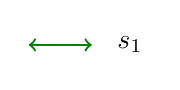
\begin{tikzpicture}[baseline=-0.5ex]
                \draw[Green, thick, <->] (0,0) -- (0.8,0);
                \node[right=0.2cm] at (0.8,0) {$s_1$};
            \end{tikzpicture}\\[0.4em]
            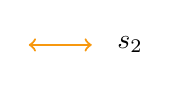
\begin{tikzpicture}[baseline=-0.5ex]
                \draw[YellowOrange, thick, <->] (0,0) -- (0.8,0);
                \node[right=0.2cm] at (0.8,0) {$s_2$};
            \end{tikzpicture}\\[0.4em]
            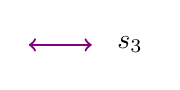
\begin{tikzpicture}[baseline=-0.5ex]
                \draw[Purple, thick, <->] (0,0) -- (0.8,0);
                \node[right=0.2cm] at (0.8,0) {$s_3$};
            \end{tikzpicture}
        };

    \end{tikzpicture}
    \caption{\texttt{6个状态之间的完全连接}}
    \label{fig:complete_state_graph}
\end{figure}

从各个变换的效果来看，对$6$个状态继续变换，结果还是在这$6$个状态之中。而且任意两个状态之间都连线了。这说明我们已经掌握了所有的状态，以及任两个状态之间如何变换。每个变换的知识，我们都能通过这个图知道。

不过，完整的图案过于复杂了。我们可以只看其中的一部分。我们再次从初始状态出发，不过这次我们只关心变换$r_1$（逆时针旋转$120^\circ$）。它把初始状态$A_1$变为$A_2$。继续用它改变$A_2$，得到$A_3$。而用它改变$A_3$则又得到$A_1$。这构成一个循环。而变换$r_2$（顺时针旋转$120^\circ$）则把$A_1$变为$A_3$，然后再变为$A_2$，最后回到$A_1$。

\vspace{12pt}
\begin{figure}[htbp]
    \centering
    \begin{tikzpicture}[>=Stealth, thick, font=\normalsize]

        % ================= 左侧：A1, A2, A3（正三角） =================
        
        \def\R{1.6}
        
        % A1 (正上方, 90度)
        \pic[scale=0.8] (A1) at (90:\R) {tri={BrickRed}{LimeGreen}{RoyalBlue}};
        \node at (A1-C) {$A_1$};
        
        % A2 (左下, -150度)
        \pic[scale=0.8] (A2) at (-150:\R) {tri={RoyalBlue}{BrickRed}{LimeGreen}};
        \node at (A2-C) {$A_2$};
        
        % A3 (右下, -30度)
        \pic[scale=0.8] (A3) at (-30:\R) {tri={LimeGreen}{RoyalBlue}{BrickRed}};
        \node at (A3-C) {$A_3$};

        % r1 (逆时针120度): 红色单向弧线 A1→A2→A3→A1
        \draw[Red, ->, thick, shorten <=15pt, shorten >=15pt] 
            ($(0,0)!1.3!(A1-C)$) to[bend right=30] ($(0,0)!1.3!(A2-C)$);
        \draw[Red, ->, thick, shorten <=15pt, shorten >=15pt] 
            ($(0,0)!1.3!(A2-C)$) to[bend right=30] ($(0,0)!1.3!(A3-C)$);
        \draw[Red, ->, thick, shorten <=15pt, shorten >=15pt] 
            ($(0,0)!1.3!(A3-C)$) to[bend right=30] ($(0,0)!1.3!(A1-C)$);

        % r2 (顺时针120度): 蓝色直线 A1→A3→A2→A1
        \draw[Blue, ->, thick, shorten <=15pt, shorten >=15pt] (A1-C) to (A3-C);
        \draw[Blue, ->, thick, shorten <=15pt, shorten >=15pt] (A3-C) to (A2-C);
        \draw[Blue, ->, thick, shorten <=15pt, shorten >=15pt] (A2-C) to (A1-C);


        % ================= 右侧：A4, A5, A6（倒三角） =================
        \begin{scope}[shift={(5.3,0.8)}]
            
            % A6 (左上, 150度)
            \pic[scale=0.8] (B6) at (150:\R) {tri={LimeGreen}{BrickRed}{RoyalBlue}};
            \node at (B6-C) {$A_6$};
            
            % A5 (右上, 30度)
            \pic[scale=0.8] (B5) at (30:\R) {tri={RoyalBlue}{LimeGreen}{BrickRed}};
            \node at (B5-C) {$A_5$};
            
            % A4 (正下方, -90度)
            \pic[scale=0.8] (B4) at (-90:\R) {tri={BrickRed}{RoyalBlue}{LimeGreen}};
            \node at (B4-C) {$A_4$};

            % r1 (逆时针120度): 红色单向弧线 A4→A6→A5→A4
            \draw[Red, ->, thick, shorten <=25pt, shorten >=25pt] 
                ($(0,0)!1.3!(B4-C)$) to ($(0,0)!1.3!(B6-C)$);
            \draw[Red, ->, thick, shorten <=25pt, shorten >=25pt] 
                ($(0,0)!1.3!(B6-C)$) to ($(0,0)!1.3!(B5-C)$);
            \draw[Red, ->, thick, shorten <=25pt, shorten >=25pt] 
                ($(0,0)!1.3!(B5-C)$) to ($(0,0)!1.3!(B4-C)$);

            % r2 (顺时针120度): 蓝色直线 A4→A5→A6→A4
            \draw[Blue, ->, thick, shorten <=15pt, shorten >=15pt] (B4-C) to (B5-C);
            \draw[Blue, ->, thick, shorten <=15pt, shorten >=15pt] (B5-C) to (B6-C);
            \draw[Blue, ->, thick, shorten <=15pt, shorten >=15pt] (B6-C) to (B4-C);
            
        \end{scope}

        % ================= 右侧图例 =================
        
        \node[font=\small, anchor=north west, align=left] at (8.3,2)
        {
            \textbf{变换图例：}\\[0.5em]
            \begin{tikzpicture}[baseline=-0.5ex]
                \draw[Red, thick, ->] (0,0) -- (0.8,0);
                \node[right=0.2cm] at (0.8,0) {$r_1$};
            \end{tikzpicture}\\[0.4em]
            \begin{tikzpicture}[baseline=-0.5ex]
                \draw[Blue, thick, ->] (0,0) -- (0.8,0);
                \node[right=0.2cm] at (0.8,0) {$r_2$};
            \end{tikzpicture}\\[0.4em]
        };

    \end{tikzpicture}
    \caption{\texttt{3个状态之间通过旋转连接构成循环}}
    \label{fig:rotation_cycles}
\end{figure}

我们也可以从状态$A_4$出发，查看旋转变换的效果。$r_1$把初始状态$A_4$变为$A_6$。继续用它改变$A_6$，得到$A_5$。而用它改变$A_5$则又得到$A_4$，构成循环。而变换$r_2$则把$A_4$变为$A_5$，然后再变为$A_6$，最后回到$A_4$。

再来看$s_1$（沿竖直中线翻转）这个变换。它把初始状态变为$A_4$。再次用它变换$A_4$，则回到初始状态$A_1$。同理，它把$A_2$和$A_5$互换，$A_3$和$A_6$互换。沿其他中线翻转，也有类似效果。

\begin{figure}[htbp]
    \centering
    \begin{tikzpicture}[>=Stealth, thick, font=\normalsize]
        
        % 设定边界
        % \path (10, -3.5) rectangle (-2, 3.5); 

        % 定义子图的水平位置
        \def\xI{0}
        \def\xII{4}
        \def\xIII{8}
        
        % 定义上下垂直位置
        \def\yTop{1.5}
        \def\yBot{-1.5}

        % ================= 子图 1: A1 -> A4 =================
        % 上方 A1
        \pic[scale=0.8] (A1) at (\xI, \yTop) {tri={BrickRed}{LimeGreen}{RoyalBlue}};
        \node at (A1-C) {$A_1$};
        
        % 下方 A4
        \pic[scale=0.8] (A4) at (\xI, \yBot) {tri={BrickRed}{RoyalBlue}{LimeGreen}};
        \node at (A4-C) {$A_4$};
        
        % 双向箭头 (s1 为绿色)
        \draw[Green, <->, thick, shorten <=15pt, shorten >=25pt] (\xI, \yTop) -- (\xI, \yBot);


        % ================= 子图 2: A2 -> A5 =================
        % 上方 A2
        \pic[scale=0.8] (A2) at (\xII, \yTop) {tri={RoyalBlue}{BrickRed}{LimeGreen}};
        \node at (A2-C) {$A_2$};
        
        % 下方 A5
        \pic[scale=0.8] (A5) at (\xII, \yBot) {tri={RoyalBlue}{LimeGreen}{BrickRed}};
        \node at (A5-C) {$A_5$};
        
        % 双向箭头
        \draw[Green, <->, thick, shorten <=15pt, shorten >=25pt] (\xII, \yTop) -- (\xII, \yBot);


        % ================= 子图 3: A3 -> A6 =================
        % 上方 A3
        \pic[scale=0.8] (A3) at (\xIII, \yTop) {tri={LimeGreen}{RoyalBlue}{BrickRed}};
        \node at (A3-C) {$A_3$};
        
        % 下方 A6
        \pic[scale=0.8] (A6) at (\xIII, \yBot) {tri={LimeGreen}{BrickRed}{RoyalBlue}};
        \node at (A6-C) {$A_6$};
        
        % 双向箭头
        \draw[Green, <->, thick, shorten <=15pt, shorten >=25pt] (\xIII, \yTop) -- (\xIII, \yBot);

    \end{tikzpicture}
    \caption{\texttt{$s_1$（竖直翻转）的效果：上方顶点不变，左下与右下顶点互换}}
    \label{fig:s1_transformation}
\end{figure}

这些图比完整的图更简单，更方便我们查看。

\section{生成与路径}

上一节我们尝试了两种方法来看清楚一个群。一种是从每个状态出发，研究所有的变换的效果。另一种是只考虑一种变换，不断重复，观察效果。前者能得到所有状态和变换的信息，但太复杂了。后者简单明了，但并不能遍历所有的状态。现在我们再换一种方法来探索：只挑最少的变换，到达所有的状态。

正三角形的对称变换有$6$个状态。如果只看旋转（比如只用$r_1$），能到达其中$3$个状态；如果只看翻转（比如只用$s_1$），能到达$2$个状态。但仔细观察可以发现，翻转能够到达旋转到不了的状态。于是我们用$s_1$和$r_1$组合，看能到达哪些状态。我们知道不断重复$r_1$变换，会把$A_1$变成$A_2$，再变成$A_3$，最后变回$A_1$。而$s_1$则把$A_1$变成$A_4$。这样，如果接着进行$r_1$变换，就会变成$A_6$、$A_5$，再回到$A_4$。最后再进行$s_1$变换，就回到$A_1$。于是，我们用$r_1,s_1$两个变换，就到达了所有的状态。

\vspace{8pt}
\begin{figure}[htbp]
    \centering
    \begin{tikzpicture}[>=Stealth, thick, font=\normalsize]

        % ================= 节点与状态 =================
        \def\R{1.6} % 六边形半径
        
        % 绘制 6 个状态节点        
        % A1 (正上方, 90度)
        \pic[scale=0.8] (A1) at (90:\R) {tri={BrickRed}{LimeGreen}{RoyalBlue}};
        \node at (A1-C) {$A_1$};
        
        % A5 (左下, -150度)
        \pic[scale=0.8] (A2) at (-150:\R) {tri={RoyalBlue}{BrickRed}{LimeGreen}};
        \node at (A2-C) {$A_2$};
        
        % A3 (右下, -30度)
        \pic[scale=0.8] (A3) at (-30:\R) {tri={LimeGreen}{RoyalBlue}{BrickRed}};
        \node at (A3-C) {$A_3$};
        % 2. r1 (逆时针120度): 红色单向弧线
        \draw[Red, ->, thick, shorten <=15pt, shorten >=15pt] (A1-C) to (A2-C);
        \draw[Red, ->, thick, shorten <=15pt, shorten >=15pt] (A2-C) to (A3-C);
        \draw[Red, ->, thick, shorten <=15pt, shorten >=15pt] (A3-C) to (A1-C);
        
        \begin{scope}[shift={(5,0)}]
            % A2 (右上, 30度)
            \pic[scale=0.8] (A5) at (-30:\R) {tri={RoyalBlue}{LimeGreen}{BrickRed}};
            \node at (A5-C) {$A_5$};
            
            % A4 (正下方, -90度)
            \pic[scale=0.8] (A4) at (90:\R) {tri={BrickRed}{RoyalBlue}{LimeGreen}};
            \node at (A4-C) {$A_4$};
            
            % A6 (左上, 150度)
            \pic[scale=0.8] (A6) at (-150:\R) {tri={LimeGreen}{BrickRed}{RoyalBlue}};
            \node at (A6-C) {$A_6$};
            % 2. r1 (逆时针120度): 红色单向弧线
            \draw[Red, ->, thick, shorten <=15pt, shorten >=15pt] (A4-C) to (A6-C);
            \draw[Red, ->, thick, shorten <=15pt, shorten >=15pt] (A5-C) to (A4-C);
            \draw[Red, ->, thick, shorten <=15pt, shorten >=15pt] (A6-C) to (A5-C);
            
        \end{scope}
        % s_1 绿色双箭头
        \draw[Green, <->, thick, shorten <=20pt, shorten >=20pt] (A1-C) -- (A4-C);

        % ================= 右侧图例 =================
        
        \node[font=\small, anchor=north west, align=left] at (7,2.4)
        {
            \textbf{变换图例：}\\[0.5em]
            \begin{tikzpicture}[baseline=-0.5ex]
                \draw[Red, thick, ->] (0,0) -- (0.8,0);
                \node[right=0.2cm] at (0.8,0) {$r_1$};
            \end{tikzpicture}\\[0.4em]
            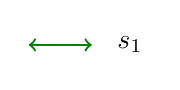
\begin{tikzpicture}[baseline=-0.5ex]
                \draw[Green, thick, <->] (0,0) -- (0.8,0);
                \node[right=0.2cm] at (0.8,0) {$s_1$};
            \end{tikzpicture}\\[0.4em]
        };

    \end{tikzpicture}
    \caption{\texttt{用两个变换到达所有状态}}
    \label{fig:two_cycles}
\end{figure}

如果我们把$r_1$制造的两个三状态的循环视为相互独立的“世界”，$s_1$就是在两个“世界”之间往返的“通道”。$A_1$和$A_4$就是“出入口”。这样的“出入口”还有$A_2$和$A_5$，$A_3$和$A_6$。只要有了这些“出入口”，就能从一个“世界”到达另一个“世界”。因此我们可以把正三角形的对称变换用下图表示。

\vspace{12pt}
\begin{figure}[htbp]
    \centering
    \begin{tikzpicture}[>=Stealth, thick, font=\normalsize]
        % ================= 节点与状态 =================
        \def\R{3.0} % 外围半径
        \def\Rt{1.1}  % 内围半径
        
        % 绘制 6 个状态节点
        
        % A1 (正上方, 90度)
        \pic[scale=0.8] (A1) at (90:\R) {tri={BrickRed}{LimeGreen}{RoyalBlue}};
        \node at (A1-C) {$A_1$};        
        % A5 (左下, -150度)
        \pic[scale=0.8] (A2) at (-150:\R) {tri={RoyalBlue}{BrickRed}{LimeGreen}};
        \node at (A2-C) {$A_2$};        
        % A3 (右下, -30度)
        \pic[scale=0.8] (A3) at (-30:\R) {tri={LimeGreen}{RoyalBlue}{BrickRed}};
        \node at (A3-C) {$A_3$};
        % r1 (逆时针120度): 红色单向弧线 A1→A2→A3→A1
        \draw[Red, ->, thick, shorten <=15pt, shorten >=15pt] 
            ($(0,0)!1.1!(A1-C)$) to[bend right=35] ($(0,0)!1.1!(A2-C)$);
        \draw[Red, ->, thick, shorten <=15pt, shorten >=15pt] 
            ($(0,0)!1.1!(A2-C)$) to[bend right=35] ($(0,0)!1.1!(A3-C)$);
        \draw[Red, ->, thick, shorten <=15pt, shorten >=15pt] 
            ($(0,0)!1.1!(A3-C)$) to[bend right=35] ($(0,0)!1.1!(A1-C)$);
        
        % A4 (正上方, 90度)
        \pic[scale=0.8] (A4) at (90:\Rt) {tri={BrickRed}{RoyalBlue}{LimeGreen}};
        \node at (A4-C) {$A_4$};
        % A2 (左下, -150度)
        \pic[scale=0.8] (A5) at (-150:\Rt) {tri={RoyalBlue}{LimeGreen}{BrickRed}};
        \node at (A5-C) {$A_5$};        
        % A6 (右下, -30度)
        \pic[scale=0.8] (A6) at (-30:\Rt) {tri={LimeGreen}{BrickRed}{RoyalBlue}};
        \node at (A6-C) {$A_6$};
        % r1 : 红色单向箭头 A4→A6→A5→A4
        \draw[Red, ->, thick, shorten <=15pt, shorten >=15pt] (A4-C) to (A6-C);
        \draw[Red, ->, thick, shorten <=15pt, shorten >=15pt] (A5-C) to (A4-C);
        \draw[Red, ->, thick, shorten <=15pt, shorten >=15pt] (A6-C) to (A5-C);

        % s1 : 绿色双向箭头
        \draw[Green, <->, thick, shorten <=10pt, shorten >=22pt] (A1-C) -- (A4-C);
        \draw[Green, <->, thick, shorten <=10pt, shorten >=22pt] (A2-C) -- (A5-C);
        \draw[Green, <->, thick, shorten <=10pt, shorten >=22pt] (A3-C) -- (A6-C);

        % ================= 右侧图例 =================
        
        \node[font=\small, anchor=north west, align=left] at (4.5,3.6)
        {
            \textbf{变换图例：}\\[0.5em]
            \begin{tikzpicture}[baseline=-0.5ex]
                \draw[Red, thick, ->] (0,0) -- (0.8,0);
                \node[right=0.2cm] at (0.8,0) {$r_1$};
            \end{tikzpicture}\\[0.4em]
            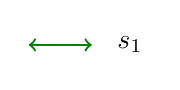
\begin{tikzpicture}[baseline=-0.5ex]
                \draw[Green, thick, <->] (0,0) -- (0.8,0);
                \node[right=0.2cm] at (0.8,0) {$s_1$};
            \end{tikzpicture}\\[0.4em]
        };

    \end{tikzpicture}
    \caption{\texttt{用两个变换描述6个状态之间的关系}}
    \label{fig:complete_state_graph}
\end{figure}

这种优美的性质只属于$r_1,s_1$吗？不然。我们可以验证，任何一个旋转变换加上任何一个翻转变换都能达到这个效果。通过观察，你应该可以解释为什么这是对的。实际上，具体用哪个变换并不重要，重要的是理解从一个变换出发，逐步添加变换，得到越来越多的状态的想法。我们说我们用$r_1, s_1$\textbf{生成}了整个群。

既然我们能用$r_1, s_1$两个变换到达所有状态，那么其他的变换就可以看作$r_1$和$s_1$的组合了。我们可以具体地写出来：
\begin{align*}
    r_2 &= r_1\rightarrow r_1, &\qquad e &= r_1\rightarrow r_1\rightarrow r_1 \\
    s_2 &= s_1\rightarrow r_1\rightarrow r_1, &\qquad s_3 &= s_1\rightarrow r_1 
\end{align*}
其中$s_1\rightarrow r_1$表示先进行$s_1$变换，再进行$r_1$变换。其余类同。把其他变换表示成$r_1, s_1$组合，称为它的\textbf{路径}。探明了路径，我们就知道如何从任一个状态到达另一个状态了。

要注意的是：到达另一个状态的路径并不唯一。比如从$A_1$到$A_5$，我们可以用$s_1\rightarrow r_1\rightarrow r_1$，也可以用$r_1\rightarrow s_1$。两个路径不同，但能到达同一个状态。

\section{长方形的群}

再来看另一个例子。这次我们考虑一个长方形。如何变换能让它的形状保持不变呢？这次我们将从单个变换开始，逐步增加变换，一步步地找出所有的状态。

首先，和三角形的例子一样，我们给长方形的四个顶点标记不同的颜色（如下图所示）。通过顶点颜色的变化，来表示长方形的对称变换。

\vspace{12pt}
\begin{figure}[htbp]
    \centering
    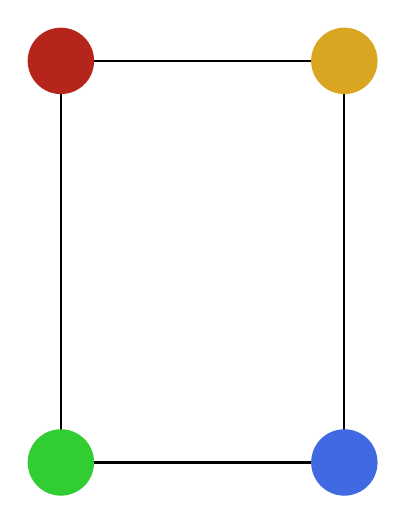
\begin{tikzpicture}
        \pic[scale=3] (R1) at (0,0) {recta={BrickRed}{LimeGreen}{RoyalBlue}{Goldenrod}};
    \end{tikzpicture}
    \label{fig:example-rectangle-1}
\end{figure}

\vspace{12pt}
首先引入第一个变换：把长方形水平翻转。它把长方形的左边和右边互换。我们称这个变换为$p$。于是我们得到了两个状态：初始状态$B_1$，以及$s$变换后的状态$B_2$。

\vspace{12pt}
\begin{figure}[htbp]
    \centering
    \begin{tikzpicture}
        \def\radius{0.3}
        \pic[scale=1] (R1) at (0,0) {recta={BrickRed}{LimeGreen}{RoyalBlue}{Goldenrod}};
        \pic[scale=1] (R2) at (5,0) {recta={Goldenrod}{RoyalBlue}{LimeGreen}{BrickRed}};
        \pic[scale=1] (R2) at (10,0) {recta={BrickRed}{LimeGreen}{RoyalBlue}{Goldenrod}};
            
        \node at (0,0) {\Large{$B_1$}};
        \node at (5,0) {\Large{$B_2$}};
        \node at (10,0) {\Large{$B_1$}};
        \node[below] at (2.5,0) {$p$};
        \node[below] at (7.5,0) {$p$};
        % 翻转轴（虚线中线）
        \draw[dashed, thick, gray] (0, 1.5) -- (0, -1.5);
        % 翻转箭头（底边下方，半圆弧）
        \draw[very thick] (0,1) ++ (180:\radius) arc (180:10:\radius); 
        \draw[-{To[length=4pt,width=3pt]}, very thick] (0,1) ++ (10:\radius) arc (20:10:\radius); 
        \draw[-Latex, very thick] (1.2,0) -- (3.8,0);
        \draw[-Latex, very thick] (6.2,0) -- (8.8,0);
    \end{tikzpicture}
    \caption{\texttt{水平翻转变换$p$的效果：左边和右边互换}}
    \label{fig:klein_horizontal_flip}
\end{figure}

继续用$p$变换$B_2$，我们发现长方形又回到了初始状态。也就是说，只用水平变换$p$，我们只能得到长方形的两个状态。

于是我们引入第二个变换：把长方形竖直翻转。它把长方形的上边和下边互换。我们称这个变换为$q$。它把长方形的初始状态$B_1$变为状态$B_3$。继续用$q$变换$B_3$，又回到初始状态。现在我们得到了$3$个状态，分别是初始状态$B_1$，水平翻转后的状态$B_2$，以及竖直翻转后的状态$B_3$。

\vspace{12pt}
\begin{figure}[htbp]
    \centering
    \begin{tikzpicture}
        \def\radius{0.3}
        \pic[scale=1] (R1) at (0,0) {recta={BrickRed}{LimeGreen}{RoyalBlue}{Goldenrod}};
        \pic[scale=1] (R2) at (5,0) {recta={Goldenrod}{RoyalBlue}{LimeGreen}{BrickRed}};
        \pic[scale=1] (R3) at (0,-4) {recta={LimeGreen}{BrickRed}{Goldenrod}{RoyalBlue}};
        \pic[scale=1] (R1) at (0,-8) {recta={BrickRed}{LimeGreen}{RoyalBlue}{Goldenrod}};
            
        % 翻转轴（虚线中线）
        \draw[dashed, thick, gray] (-1.3, 0) -- (1.1,0);
        % 翻转箭头（底边下方，半圆弧）
        \draw[very thick] (-0.9,0) ++ (-90:\radius) arc (260:90:\radius); 
        \draw[-{To[length=4pt,width=3pt]}, very thick] (-0.9,0) ++ (-90:\radius) arc (-110:-100:\radius); 
        \node at (0,0) {\Large{$B_1$}};
        \node at (5,0) {\Large{$B_2$}};
        \node at (0,-4) {\Large{$B_3$}};
        \node at (0,-8) {\Large{$B_1$}};
        \node[below] at (2.5,0) {$p$};
        \node[right] at (0,-2) {$q$};
        \node[right] at (0,-6) {$q$};
        % 翻转轴（虚线中线）
        \draw[dashed, thick, gray] (2.5, 1.2) -- (2.5, 0.2);
        % 翻转箭头（底边下方，半圆弧）
        \draw[very thick] (2.5,0.6) ++ (180:\radius) arc (180:10:\radius); 
        \draw[-{To[length=4pt,width=3pt]}, very thick] (2.5,0.6) ++ (10:\radius) arc (20:10:\radius); 
        \draw[Latex-Latex, very thick] (1.2,0) -- (3.8,0);
        \draw[-Latex, very thick] (0,-1.1) -- (0,-2.9);
        \draw[-Latex, very thick] (0,-5.1) -- (0,-6.9);
    \end{tikzpicture}
    \caption{\texttt{竖直翻转变换$q$的效果：上边和下边互换}}
    \label{fig:klein_vertical_flip}
\end{figure}

\vspace{12pt}
水平翻转变换$p$和竖直翻转变换$q$分别把初始状态带到了$B_2$和$B_3$。但继续水平翻转$B_2$、竖直翻转$B_3$，只会回到初始状态。不过，我们还有别的方法来变换它们，就是竖直翻转$B_2$、水平翻转$B_3$。我们来看看会发生什么。

\vspace{12pt}
\begin{figure}[htbp]
    \centering
    \begin{tikzpicture}
        \def\radius{0.3}
        \pic[scale=1] (R1) at (0,0) {recta={Goldenrod}{RoyalBlue}{LimeGreen}{BrickRed}};
        \pic[scale=1] (R2) at (5,0) {recta={RoyalBlue}{Goldenrod}{BrickRed}{LimeGreen}};
        \pic[scale=1] (R1) at (0,-4) {recta={LimeGreen}{BrickRed}{Goldenrod}{RoyalBlue}};
        \pic[scale=1] (R2) at (5,-4) {recta={RoyalBlue}{Goldenrod}{BrickRed}{LimeGreen}};
            
        \node at (0,0) {\Large{$B_2$}};
        \node at (0,-4) {\Large{$B_3$}};
        \node[below] at (2.5,0) {$q$};
        \node[below] at (2.5,-4) {$p$};
        % 翻转轴（虚线中线）
        \draw[dashed, thick, gray] (-1.3, 0) -- (1.1,0);
        % 翻转箭头（底边下方，半圆弧）
        \draw[very thick] (-0.9,0) ++ (-90:\radius) arc (260:90:\radius); 
        \draw[-{To[length=4pt,width=3pt]}, very thick] (-0.9,0) ++ (-90:\radius) arc (-110:-100:\radius); 
        
        % 翻转轴（虚线中线）
        \draw[dashed, thick, gray] (0, 1.5-4) -- (0, -1.5-4);
        % 翻转箭头（底边下方，半圆弧）
        \draw[very thick] (0,1-4) ++ (180:\radius) arc (180:10:\radius); 
        \draw[-{To[length=4pt,width=3pt]}, very thick] (0,1-4) ++ (10:\radius) arc (20:10:\radius); 
        \draw[-Latex, very thick] (1.2,0) -- (3.8,0);
        \draw[-Latex, very thick] (1.2,-4) -- (3.8,-4);
    \end{tikzpicture}
    \caption{\texttt{水平翻转$B_2$与竖直翻转$B_3$的效果相同}}
    \label{fig:klein_combined_flip}
\end{figure}

\vspace{12pt}
我们看到，水平翻转$B_2$与竖直翻转$B_3$的效果是相同的。我们得到了一个新状态$B_4$。而继续对$B_4$进行水平翻转和竖直翻转，得到的都还是$B_2$和$B_3$。这说明这四个状态就是我们用$p$和$q$两个变换能得到的所有状态。我们可以把它们画在一个图上。

\vspace{12pt}
\begin{figure}[htbp]
    \centering
    \begin{tikzpicture}
        \def\radius{0.3}
        \pic[scale=1] (R1) at (0,0) {recta={BrickRed}{LimeGreen}{RoyalBlue}{Goldenrod}};
        \pic[scale=1] (R2) at (5,0) {recta={Goldenrod}{RoyalBlue}{LimeGreen}{BrickRed}};
        \pic[scale=1] (R1) at (0,-4) {recta={LimeGreen}{BrickRed}{Goldenrod}{RoyalBlue}};
        \pic[scale=1] (R2) at (5,-4) {recta={RoyalBlue}{Goldenrod}{BrickRed}{LimeGreen}};

        \node at (0,0) {\Large{$B_1$}};
        \node at (5,0) {\Large{$B_2$}};
        \node at (0,-4) {\Large{$B_3$}};
        \node at (5,-4) {\Large{$B_4$}};
        \node[below] at (2.5,0) {$p$};
        \node[below] at (2.5,-4) {$p$};
        \node[right] at (0,-2) {$q$};
        \node[left] at (5,-2) {$q$};
        % 翻转轴（虚线中线）
        \draw[dashed, thick, gray] (2.5, 1.2) -- (2.5, 0.2);
        % 翻转箭头（底边下方，半圆弧）
        \draw[very thick] (2.5,0.6) ++ (180:\radius) arc (180:10:\radius); 
        \draw[-{To[length=4pt,width=3pt]}, very thick] (2.5,0.6) ++ (10:\radius) arc (20:10:\radius); 
        % 翻转轴（虚线中线）
        \draw[dashed, thick, gray] (2.5, 1.2-4) -- (2.5, 0.2-4);
        % 翻转箭头（底边下方，半圆弧）
        \draw[very thick] (2.5,0.6-4) ++ (180:\radius) arc (180:10:\radius); 
        \draw[-{To[length=4pt,width=3pt]}, very thick] (2.5,0.6-4) ++ (10:\radius) arc (20:10:\radius); 
        % 翻转轴（虚线中线）
        \draw[dashed, thick, gray] (-1.3, -2) -- (-0.3,-2);
        % 翻转箭头（底边下方，半圆弧）
        \draw[very thick] (-0.9,-2) ++ (-90:\radius) arc (260:90:\radius); 
        \draw[-{To[length=4pt,width=3pt]}, very thick] (-0.9,-2) ++ (-90:\radius) arc (-110:-100:\radius); 
        % 翻转轴（虚线中线）
        \draw[dashed, thick, gray] (5+1.3, -2) -- (5+0.3,-2);
        % 翻转箭头（底边下方，半圆弧）
        \draw[very thick] (5+0.9,-2) ++ (-90:\radius) arc (260:90:\radius); 
        \draw[-{To[length=4pt,width=3pt]}, very thick] (5+0.9,-2) ++ (-90:\radius) arc (-110:-100:\radius); 
        \draw[Latex-Latex, very thick] (1.2,0) -- (3.8,0);
        \draw[Latex-Latex, very thick] (0,-1.1) -- (0,-2.9);
        \draw[Latex-Latex, very thick] (1.2,-4) -- (3.8,-4);
        \draw[Latex-Latex, very thick] (5,-1.1) -- (5,-2.9);
    \end{tikzpicture}
    \caption{\texttt{用$p$和$q$两个变换得到的$4$个状态的关系}}
    \label{fig:klein_combined_flip}
\end{figure}

这$4$个状态是否就是使得长方形形状保持不变的所有状态呢？的确如此。我们可以用顶点的颜色来证明：

首先考虑红色顶点，它只能出现在长方形$4$个顶点中的一个顶点上，于是有$4$种可能。一旦红色顶点位置确定，那么黄色顶点必然在它相邻的短边的另一端，绿色顶点必然在它相邻的长边的另一端，而剩下只有一个顶点，就是蓝色顶点的位置。因此，所有状态只有$4$个，通过变换$p,q$，我们已经把它们全部找到了。

以上就是通过不断添加变换生成群的方法。我们把用这种方法生成的图称为群的\textbf{生成路径图}。它清楚地显示了群里的变换和各个状态之间的关系。如果你觉得三角形和长方形的对称变换构成的群都太简单了，可以试着用这种方法来研究正方体的旋转构成的群。它比三角形和长方形的例子要复杂不少。如果遇到困难，可以参考附录中的解答。

群的生成路径图显然不是唯一的。它只是一种遍历状态的方法。群的生成路径图仿佛是一张地图。它告诉我们从一个状态出发，经过哪些变换，就能到达另一个状态，指出状态之间的路径。

你也许会说：如何保证我们穷尽了所有的状态呢？实际上，生成路径图并不保证我们穷尽了所有状态。相反，一旦我们发现了一个不在图中的新状态，它必然是我们已知的变换无法达到的（因为之前我们已经穷尽了已知变换所能达到的所有状态）。于是，通过理解它如何从已知状态得来，我们就能扩大我们的地图，生成更多的路径。这就是生成路径图的理念。我们也可以说，生成路径图表示我们已知的变换能生成的群的面貌。

\section{共同的结构}

群之所以重要，在于它提炼了不同现象之间的共同性质。比起具体例子中的状态，我们更关心状态之间的变换。变换体现了对称的规律。

比如，我们可以考虑队列操演时原地“向右转”、“向后转”、“向左转”、“立正”这$4$个动作。这些动作效果确定，可以恢复（比如向左转再向右转就回到原来的状态），组合后没有新动作（比如向右转再向后转就是向左转，等等），所以构成一个群。

\vspace{8pt}
\begin{figure}[htbp]
    \centering
    \begin{tikzpicture}[>=Stealth, thick, font=\normalsize]
        % 循环群：C_4
        \begin{scope}[scale=0.8]
            \def\R{1.6}
            \def\initialtheta{90}
            \def\n{4}
            \def\abend{25}
            \node[circle, draw=black, minimum size=30] (n0) at (\initialtheta-0*360/\n:2) {};
            \node[circle, draw=black, minimum size=30] (n1) at (\initialtheta-1*360/\n:2) {};
            \node[circle, draw=black, minimum size=30] (n2) at (\initialtheta-2*360/\n:2) {};
            \node[circle, draw=black, minimum size=30] (n3) at (\initialtheta-3*360/\n:2) {};
            \draw[-{Latex[length=3mm,width=2mm]}, red, very thick, >=latex] (n0) to[bend left=\abend] (n1);
            \draw[-{Latex[length=3mm,width=2mm]}, red, very thick, >=latex] (n1) to[bend left=\abend] (n2);
            \draw[-{Latex[length=3mm,width=2mm]}, red, very thick, >=latex] (n2) to[bend left=\abend] (n3);
            \draw[-{Latex[length=3mm,width=2mm]}, red, very thick, >=latex] (n3) to[bend left=\abend] (n0);
            \filldraw[gray] (n0) ellipse (8pt and 3pt);
            \filldraw (n0) ++ (0, 0.1) circle (4pt);
            \filldraw[gray] (n1) ellipse (3pt and 8pt);
            \filldraw (n1) ++ (0.1, 0) circle (4pt);
            \filldraw[gray] (n2) ellipse (8pt and 3pt);
            \filldraw (n2) ++ (0, -0.1) circle (4pt);
            \filldraw[gray] (n3) ellipse (3pt and 8pt);
            \filldraw (n3) ++ (-0.1, 0) circle (4pt);
        \end{scope}
        
    \end{tikzpicture}
    \caption{\texttt{向右转$4$次回到原本状态}}
    \label{fig:four-cycles}
\end{figure}

以身体向前作为初始状态，这些动作把身体状态顺次变成向前、向右、向后、向左。因此，一共有$4$个状态，和长方形的对称变换构成的群一样。

但是，我们发现，这两个群的结构不相同。长方形的变换群里，所有变换重复$2$次之后都回到原状态。即便是$B_1$到$B_4$的变换，再重复一次也回到$B_1$。但是我们知道，向右转$4$次后，才会回到原来的站位。所以，长方体的对称变换里，没有和“向右转”一样的变换。

另一方面，我们可以考虑这样的例子：墙上有甲乙两个开关，分别控制一盏电灯。每个开关都有两个状态：开和关。因此两个开关一共有四种状态。它们可以通过拨动甲开关和拨动乙开关来达到。我们可以据此画出对应的群的生成路径图。

\vspace{12pt}
\begin{figure}[htbp]
    \centering
    \begin{tikzpicture}
        
        % 两个开关都开
        % 上开关
        \draw (-0.6, -1.1) rectangle (1.8, 0.8);
        \draw[rounded corners=3, fill=white, drop shadow={opacity=0.3, shadow xshift=0.1cm, shadow yshift=-0.1cm}]
        (0,0) rectangle (1.2,0.5);
        % 按钮（圆形）
        \filldraw[fill=white, draw=Red!30!YellowOrange, very thick, drop shadow={opacity=0.3, shadow xshift=0.05cm, shadow yshift=-0.05cm, color=Orange}] 
            (0.3,0.25) circle (0.2);
        \draw[very thick, gray!70] (0.7, 0.25) -- (1.0, 0.25);

        % 下开关
        \begin{scope}[shift={(0, -0.8)}]
            
            \draw[rounded corners=3, fill=white, drop shadow={opacity=0.3, shadow xshift=0.1cm, shadow yshift=-0.1cm}]
            (0,0) rectangle (1.2,0.5);
            % 按钮（圆形）
            \filldraw[fill=white, draw=RoyalBlue!30!SkyBlue, very thick, drop shadow={opacity=0.3, shadow xshift=0.05cm, shadow yshift=-0.05cm, color=RoyalBlue}] 
                (0.3,0.25) circle (0.2);
            \draw[very thick, gray!70] (0.7, 0.25) -- (1.0, 0.25);
        \end{scope}
        
        % 上关下开
        \begin{scope}[shift={(5,0)}]
            \draw (-0.6, -1.1) rectangle (1.8, 0.8);
            \draw[rounded corners=3, fill=white, drop shadow={opacity=0.3, shadow xshift=0.1cm, shadow yshift=-0.1cm}]
            (0,0) rectangle (1.2,0.5);
            % 按钮（圆形）
            \filldraw[fill=white, draw=gray!70, very thick] 
                (0.3,0.25) circle (0.2);
            \draw[very thick, gray!70] (0.7, 0.25) -- (1.0, 0.25);

            \begin{scope}[shift={(0, -0.8)}]
                \draw[rounded corners=3, fill=white, drop shadow={opacity=0.3, shadow xshift=0.1cm, shadow yshift=-0.1cm}]
                (0,0) rectangle (1.2,0.5);
                % 按钮（圆形）
                \filldraw[fill=white, draw=RoyalBlue!30!SkyBlue, very thick, drop shadow={opacity=0.3, shadow xshift=0.05cm, shadow yshift=-0.05cm, color=RoyalBlue}] 
                    (0.3,0.25) circle (0.2);
                \draw[very thick, gray!70] (0.7, 0.25) -- (1.0, 0.25);
            \end{scope}        
        \end{scope}
        
        % 上开下关
        \begin{scope}[shift={(0, -4)}]
            \draw (-0.6, -1.1) rectangle (1.8, 0.8);
            \draw[rounded corners=3, fill=white, drop shadow={opacity=0.3, shadow xshift=0.1cm, shadow yshift=-0.1cm}]
            (0,0) rectangle (1.2,0.5);
            % 按钮（圆形）
            \filldraw[fill=white, draw=Red!30!YellowOrange, very thick, drop shadow={opacity=0.3, shadow xshift=0.05cm, shadow yshift=-0.05cm, color=Orange}] 
                (0.3,0.25) circle (0.2);
            \draw[very thick, gray!70] (0.7, 0.25) -- (1.0, 0.25);

            \begin{scope}[shift={(0, -0.8)}]
                \draw[rounded corners=3, fill=white, drop shadow={opacity=0.3, shadow xshift=0.1cm, shadow yshift=-0.1cm}]
                (0,0) rectangle (1.2,0.5);
                % 按钮（圆形）
                \filldraw[fill=white, draw=gray!70, very thick] 
                    (0.3,0.25) circle (0.2);
                \draw[very thick, gray!70] (0.7, 0.25) -- (1.0, 0.25);
            \end{scope}        
        \end{scope}
        
        % 两个开关都关
        \begin{scope}[shift={(5, -4)}]
            \draw (-0.6, -1.1) rectangle (1.8, 0.8);
            \draw[rounded corners=3, fill=white, drop shadow={opacity=0.3, shadow xshift=0.1cm, shadow yshift=-0.1cm}]
            (0,0) rectangle (1.2,0.5);
            % 按钮（圆形）
            \filldraw[fill=white, draw=gray!70, very thick] 
                (0.3,0.25) circle (0.2);
            \draw[very thick, gray!70] (0.7, 0.25) -- (1.0, 0.25);

            \begin{scope}[shift={(0, -0.8)}]
                \draw[rounded corners=3, fill=white, drop shadow={opacity=0.3, shadow xshift=0.1cm, shadow yshift=-0.1cm}]
                (0,0) rectangle (1.2,0.5);
                % 按钮（圆形）
                \filldraw[fill=white, draw=gray!70, very thick] 
                    (0.3,0.25) circle (0.2);
                \draw[very thick, gray!70] (0.7, 0.25) -- (1.0, 0.25);
            \end{scope}        
        \end{scope}

        \draw[Orange, Latex-Latex, very thick] (2,0) -- (4.2,0);
        \draw[RoyalBlue, Latex-Latex, very thick] (0.6,-1.3) -- (0.6,-3);
        \draw[Orange, Latex-Latex, very thick] (2,-4) -- (4.2,-4);
        \draw[RoyalBlue, Latex-Latex, very thick] (5.6,-1.3) -- (5.6,-3);
        
    \end{tikzpicture}
    \label{fig:2-switch-cayley}
    \caption{\texttt{两个开关的状态图}}
\end{figure}

可以看到，长方形的四种状态对应两个开关的四种状态，而“水平翻转”、“垂直翻转”则对应着“按上面的开关”和“按下面的开关”。如果我们不关注状态的具体内容，只关心箭头的位置和方向，那么我们会发现，这里这些箭头连接状态的方式，和前面长方形的例子是一样的。两个图的结构一致。

所以，这两个群尽管表面上不同，说的是不同的事情，但论及变换的结构，并没有不同。它们反应了两个不同事物的共同本质。我们还可以把两个开关换成两枚硬币，结果也是一样的。

变换的路径图为我们揭示了一种抽象的规律。数学上，我们说这是一种结构上的等同关系。长方体的对称变换构成的群，和两个开关的变换构成的群\textbf{同构}。我们认为，这两个群是一样的结构。讨论这个群就等于讨论那个群，讨论那个群就等于讨论这个群，没有任何区别。这个抽象的群，我们称它为\textbf{矩群}，记作$\mathsf{J}_4$。

我们只想讨论群。所以，我们可以忽略各个例子里与群无关的东西。比如说，每个状态具体是什么，究竟是两个开关、两枚硬币还是一个长方形，其实不重要。我们就说它是一个节点，用一个圆点代替。而变换就是从一个节点指向另一个节点的箭头。变换的具体意义也不重要，重要的是变换之间的关系。即两个变换组合起来是哪个变换。于是我们可以为矩群画出以下的图：

\vspace{12pt}
\begin{figure}[htbp]
    \centering
    \begin{tikzpicture}[scale=0.8,>=Latex, thick]
        \def\R{0.7}
        \def\Dx{5}
        \def\Dy{4}
        \filldraw[gray!20, draw=gray!70] (0, 0) circle (\R);
        \filldraw[gray!20, draw=gray!70] (0, -\Dy) circle (\R);
        \filldraw[gray!20, draw=gray!70] (\Dx, 0) circle (\R);
        \filldraw[gray!20, draw=gray!70] (\Dx, -\Dy) circle (\R);
        \draw[Orange, <->, very thick] (\R,0) -- (\Dx-\R,0);
        \draw[RoyalBlue, <->, very thick] (0,-\R) -- (0,\R-\Dy);
        \draw[Orange, <->, very thick] (\R,-\Dy) -- (\Dx-\R,-\Dy);
        \draw[RoyalBlue, <->, very thick] (\Dx,-\R) -- (\Dx,\R-\Dy);
        \node[above] at (.5 * \Dx,0) {$p$};
        \node[below] at (.5 * \Dx,-\Dy) {$p$};
        \node[left] at (0,-.5 * \Dy) {$q$};
        \node[right] at (\Dx,-.5 * \Dy) {$q$};
    \end{tikzpicture}
    \label{fig:V_4-cayley}
    \caption{\texttt{矩群的生成路径图}}
\end{figure}

\vspace{12pt}
矩群由两个变换$p,q$生成。我们不关心这里的$p,q$是什么变换。我们只需要知道，$p$和$q$各自重复两次就相当于什么都不走，得到恒等变换$e$。它们组合起来则是另一个变换$r$，而且不依赖于组合的顺序：
$$ r \;=\; p\rightarrow q \;=\; q\rightarrow p. $$
而$r$重复两次，也相当于什么都不做。这些关系就是我们从不同的例子里抽离出来的共性。研究这个抽象的群，得到的知识，就能应用到这些不同的例子里。比如，我们会发现：
$$ p\rightarrow q\rightarrow p = q, \qquad q\rightarrow p \rightarrow q = p. $$
因为从左上角的节点开始，往右、往下、再往左，就得到左下角的节点，效果和直接往下一样。同理，从左上角的节点开始，往下、往右、再往上，就得到右上角的节点，效果和直接往右一样。这个性质反映到开关的例子里，就是按一个开关两次的间隔里按另一个开关，和只按另一个开关效果相同。反应到长方形的例子里，就是水平翻转两次的间隔里垂直翻转一次，效果和只垂直翻转一次一样。一旦掌握了抽象的本质，我们就能用它理解各个具体例子的相关性质。

正三角形的例子也能变成抽象的群。我们忽略正三角形的各种状态，只考虑变换之间的关系，可以画出以下的图：

\vspace{12pt}
\begin{figure}[htbp]
    \centering
    \begin{tikzpicture}[>=Stealth, thick, font=\normalsize]
        % ================= 节点与状态 =================
        \def\r{0.5}
        \def\R{3.0} % 外围半径
        \def\Rt{1.1}  % 内围半径
        
        % 绘制 6 个状态节点
        \coordinate (A1-C) at (90:\R);
        \coordinate (A3-C) at (-30:\R);
        \coordinate (A2-C) at (-150:\R);
        \coordinate (A4-C) at (90:\Rt);
        \coordinate (A6-C) at (-30:\Rt);
        \coordinate (A5-C) at (-150:\Rt);

        \filldraw[gray!20, draw=gray!70, thick] (A1-C) circle (\r);
        \filldraw[gray!20, draw=gray!70, thick] (A2-C) circle (\r);
        \filldraw[gray!20, draw=gray!70, thick] (A3-C) circle (\r);
        \filldraw[gray!20, draw=gray!70, thick] (A4-C) circle (\r);
        \filldraw[gray!20, draw=gray!70, thick] (A5-C) circle (\r);
        \filldraw[gray!20, draw=gray!70, thick] (A6-C) circle (\r);
        % r1 (逆时针120度): 红色单向弧线 A1→A2→A3→A1
        \draw[Red, ->, thick, shorten <=15pt, shorten >=15pt] 
            ($(0,0)!1.1!(A1-C)$) to[bend right=35] ($(0,0)!1.1!(A2-C)$);
        \draw[Red, ->, thick, shorten <=15pt, shorten >=15pt] 
            ($(0,0)!1.1!(A2-C)$) to[bend right=35] ($(0,0)!1.1!(A3-C)$);
        \draw[Red, ->, thick, shorten <=15pt, shorten >=15pt] 
            ($(0,0)!1.1!(A3-C)$) to[bend right=35] ($(0,0)!1.1!(A1-C)$);
        % r1 : 红色单向箭头 A4→A6→A5→A4
        \draw[Red, ->, thick, shorten <=15pt, shorten >=15pt] (A4-C) to (A6-C);
        \draw[Red, ->, thick, shorten <=15pt, shorten >=15pt] (A5-C) to (A4-C);
        \draw[Red, ->, thick, shorten <=15pt, shorten >=15pt] (A6-C) to (A5-C);

        % s1 : 绿色双向箭头
        \draw[Green, <->, thick, shorten <=15pt, shorten >=15pt] (A1-C) -- (A4-C);
        \draw[Green, <->, thick, shorten <=15pt, shorten >=15pt] (A2-C) -- (A5-C);
        \draw[Green, <->, thick, shorten <=15pt, shorten >=15pt] (A3-C) -- (A6-C);

        % ================= 右侧图例 =================
        
        \node[font=\small, anchor=north west, align=left] at (4.5,3.6)
        {
            \textbf{变换图例：}\\[0.5em]
            \begin{tikzpicture}[baseline=-0.5ex]
                \draw[Red, thick, ->] (0,0) -- (0.8,0);
                \node[right=0.2cm] at (0.8,0) {$r_1$};
            \end{tikzpicture}\\[0.4em]
            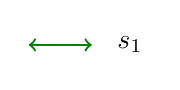
\begin{tikzpicture}[baseline=-0.5ex]
                \draw[Green, thick, <->] (0,0) -- (0.8,0);
                \node[right=0.2cm] at (0.8,0) {$s_1$};
            \end{tikzpicture}\\[0.4em]
        };

    \end{tikzpicture}
    \caption{\texttt{用两个变换描述6个状态之间的关系}}
    \label{fig:s3-cayley}
\end{figure}

\vspace{12pt}
这是一个$6$个节点，由两个变换生成的群。我们不需要知道节点的具体含义，也不需要知道$r_1$和$s_1$的具体意义。从图中我们可以看到，$r_1$重复三次总回到原节点，而$s_1$重复两次就回到原节点，等等。我们把这个群叫做\textbf{三元对称群}，记作$\mathsf{D}_3$。

\vspace{12pt}
\begin{figure}[htbp]
    \centering
    \begin{tikzpicture}[>=Stealth, thick, font=\normalsize]
        % ================= 节点与状态 =================
        \def\r{0.5}
        \def\R{3.0} % 外围半径
        \def\Rt{1.1}  % 内围半径
        
        % 绘制 6 个状态节点
        \coordinate (A1-C) at (90:\R);
        \coordinate (A3-C) at (-30:\R);
        \coordinate (A2-C) at (-150:\R);
        \coordinate (A4-C) at (90:\Rt);
        \coordinate (A6-C) at (-30:\Rt);
        \coordinate (A5-C) at (-150:\Rt);

        \filldraw[gray!20, draw=gray!70, thick] (A1-C) circle (\r);
        \filldraw[gray!20, draw=gray!70, thick] (A2-C) circle (\r);
        \filldraw[gray!20, draw=gray!70, thick] (A3-C) circle (\r);
        \filldraw[gray!20, draw=gray!70, thick] (A4-C) circle (\r);
        \filldraw[gray!20, draw=gray!70, thick] (A5-C) circle (\r);
        \filldraw[gray!20, draw=gray!70, thick] (A6-C) circle (\r);
        \node at (A1-C) {$e$};
        \node at (A2-C) {$r_1$};
        \node at (A3-C) {$r_2$};
        \node at (A4-C) {$s_1$};
        \node at (A6-C) {$s_2$};
        \node at (A5-C) {$s_3$};
        % r1 (逆时针120度): 红色单向弧线 A1→A2→A3→A1
        \draw[Red, ->, thick, shorten <=15pt, shorten >=15pt] 
            ($(0,0)!1.1!(A1-C)$) to[bend right=35] ($(0,0)!1.1!(A2-C)$);
        \draw[Red, ->, thick, shorten <=15pt, shorten >=15pt] 
            ($(0,0)!1.1!(A2-C)$) to[bend right=35] ($(0,0)!1.1!(A3-C)$);
        \draw[Red, ->, thick, shorten <=15pt, shorten >=15pt] 
            ($(0,0)!1.1!(A3-C)$) to[bend right=35] ($(0,0)!1.1!(A1-C)$);
        % r1 : 红色单向箭头 A4→A6→A5→A4
        \draw[Red, ->, thick, shorten <=15pt, shorten >=15pt] (A4-C) to (A6-C);
        \draw[Red, ->, thick, shorten <=15pt, shorten >=15pt] (A5-C) to (A4-C);
        \draw[Red, ->, thick, shorten <=15pt, shorten >=15pt] (A6-C) to (A5-C);

        % s1 : 绿色双向箭头
        \draw[Green, <->, thick, shorten <=15pt, shorten >=15pt] (A1-C) -- (A4-C);
        \draw[Green, <->, thick, shorten <=15pt, shorten >=15pt] (A2-C) -- (A5-C);
        \draw[Green, <->, thick, shorten <=15pt, shorten >=15pt] (A3-C) -- (A6-C);

    \end{tikzpicture}
    \caption{$\mathsf{D}_3$：\texttt{用变换标记$6$个状态}}
    \label{fig:s3-cayley}
\end{figure}

\vspace{12pt}
既然在生成路径图里，我们关心的是图中各个状态的关系，如何用群中的变换把状态改变。这些状态可以只看作节点，它本身是什么，我们反倒不那么关心。那么，我们可以用变换的名字来标记生成路径图里的状态节点，更方便我们理解群的结构。

具体来说，我们选定一个状态，从它出发，沿着变换构成的路径，把能到达的状态都标为这些变换复合的结果。我们把原状态视为“什么都不做”的结果，标记为$e$。然后把从$e$出发，一次变换能到达的状态，用这些变换的名字来标记。接下来再从这些状态出发，把再经历一次变换能到达的状态，用两次变换的乘积标记，等等。一个状态并不一定只有一种方法到达，我们希望给它一个简便的记法，比如可以给它起一个新名字。新的名字就意味着这个变换和之前的变换都不同。

这样，我们就标记出了群中所有的变换。这种关系是一一对应的。首先每个变换必然都通过至少一个路径到达，因此必然对应某个状态节点。其次，同一个节点对应同样的变换，于是至多有一个名字。于是，群的生成路径图里，把各个状态节点用群的元素（变换）来标记，就能标出群的所有元素（变换）。换句话说，状态节点个数有限时，就是群中变换的个数：图中有多少个状态节点，就说明群里有多少个变换。

要注意的是：这种标记方法不依赖最初选择的状态节点。从任意一个节点出发，都能完成标记。这也是群的生成路径图的特有性质。群的变换之间的对称关系，决定了我们可以这么做。反之，随便用一些节点连成的图，是不具备这种性质的。


\clearpage

\section*{本章小结}

本章我们引入了“连线图”的方法来显示群的结构。本章的主要内容包括：
\begin{itemize}
    \item \textbf{生成元与生成路径图}：我们不需要罗列所有变换，而是寻找少数几个“生成元”，通过它们不断组合的路径，遍历群的所有状态。
    \item \textbf{矩群}$\mathsf{J}_4$：它有$4$个元素，可以通过其中两个翻转变换组合得出。
    \item \textbf{三元对称群}$\mathsf{D}_3$：它有$6$个元素，可以通过其中一个旋转变换和一个翻转变换组合得出。
    \item \textbf{同构}：我们发现，长方形翻转、开关拨动、队列转向等截然不同的物理现象，其背后的状态图结构却完全一致。这种剥离了具体场景后，在抽象结构上完全等同的关系，称为“同构”。
    \item 生成路径图的状态节点和群的变换一一对应。
\end{itemize}

\clearpage
\section{练习}

\begin{problemlist}
    \item 为以下的群列出变换能实现的所有状态，然后给出生成这些状态的方法。
    \begin{problemlist}
        \item 单个硬币的翻转变换构成的群。
        \item $k$个硬币的翻转变换构成的群。
        \item 整数集的加法群（由所有“加几”操作构成的群）。
    \end{problemlist}
    \item 如何为以上的群画出生成路径图？
    \item 考虑平面中一个正方形。允许将它旋转、翻转。我们希望研究有哪些变换让它的位置和形状不变。

        \vspace{12pt}
        \begin{figure}[htbp]
            \centering        
            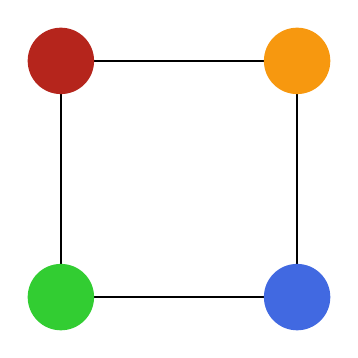
\begin{tikzpicture}
                \def\r{3}
                \def\ca{BrickRed}
                \def\cb{LimeGreen}
                \def\cc{RoyalBlue}
                \def\cd{YellowOrange}
                \begin{scope}
                    \pic at (0,0) {fang={\ca}{\cb}{\cc}{\cd}{\r}};
                \end{scope}            
            \end{tikzpicture}
        \end{figure}
        \label{fig:a-square}
    \begin{problemlist}
        \item 将正方形的四个顶点染成两两不同的颜色，比如：红、绿、黄、蓝。四个顶点所有可能的颜色组合有几种？
        \item 考虑将正方形按其中心旋转。哪些旋转变换保持其位置形状不变？这时候的顶点颜色如何变化？列出所有可能达到的状态。
        \item 考虑将正方形按过中心的轴线翻转。哪些翻转方法保持其位置形状不变？这时候的顶点颜色如何变化？列出所有可能达到的状态。
        \item 画出以上状态的生成路径图。
        \item 哪些颜色组合无法通过旋转、翻转形成？为什么？给出你的解释。
    \end{problemlist}
    \item 本题的目的是初步研究正方体的旋转对称群（记为$\mathsf{T}_6$）。思考本题时最好准备一个骰子或类似的正方体物件，最好各个面有区别，或者顶点做好了标记，通过实际上手转动正方体，理解它在空间中的旋转。我们考虑$\mathsf{T}_6$中两个变换：“朝前转动$90^\circ$，左右面不变”（记为$\tau$）和“往左转动$90^\circ$，前后面不变”（记为$\sigma$）。

    \vspace{12pt}
    \begin{figure}[htbp]
        \centering        
        \begin{tikzpicture}
            \def\r{1}
            \def\dx{2.8}
            \def\dy{1.25}
            \def\ax{0.27}
            \def\ay{-0.35}
            \def\va{BrickRed}
            \def\vb{ForestGreen}
            \def\vc{MidnightBlue}
            \def\vd{YellowOrange}
            \def\ca{SkyBlue}
            \def\cb{Yellow}
            \def\cc{Lavender}
            \def\cd{LimeGreen}
            \def\rr{0.6}
            \begin{scope}
            \draw[thick, densely dashed, Blue!70!gray] (-1.3*\dx*\r*\ax,-1.3*\dx*\r*\ay) -- (0,0);
            \draw[thick, densely dashed, Blue!70!gray] (0.6*\dx*\r,0) -- (1.8*\dx*\r,0);
            % No.1 (1 2 3 4 5 6 7 8)
            \pic at (0*\dx*\r,0*\dy*\r) {cube={\va}{\vb}{\vc}{\vd}{\ca}{\cb}{\cc}{\cd}{\r}};
            % No.1 (1 2 3 4 5 6 7 8)
            \pic at (1.2*\dx*\r,0*\dy*\r) {cube={\va}{\vb}{\vc}{\vd}{\ca}{\cb}{\cc}{\cd}{\r}};
            
            % No.15 (5 1 4 8 6 2 3 7) 朝前翻滚90度
            \pic at (2.4*\dx*\r,0*\dy*\r) {cube={\ca}{\va}{\vd}{\cd}{\cb}{\vb}{\vc}{\cc}{\r}};
            % No.11 (4 1 2 3 8 5 6 7) 朝左翻滚90度
            \pic at (-1.2*\dx*\r,0*\dy*\r) {cube={\vd}{\va}{\vb}{\vc}{\cd}{\ca}{\cb}{\cc}{\r}};
            \draw[thick, densely dashed, Blue!70!gray] (0,0) -- (1.3*\dx*\r*\ax,1.3*\dx*\r*\ay);
            \draw[very thick, RoyalBlue] (-0.22*\dx*\r+0.06,0.35*\r + \rr) arc [start angle=83, end angle=180, radius=\rr];
            \draw[-Latex,RoyalBlue,thick](-0.22*\dx*\r-\rr,0.35*\r-0.02) -- (-0.22*\dx*\r-\rr,0.35*\r-0.12);
            \end{scope}
            \begin{scope}[shift={(1.2*\dx*\r,0.3*\r)},rotate=180-84.895]
            \draw[very thick, RoyalBlue] ({1.0635*\rr*cos(23)}, {0.2539*\rr*sin(23)}) arc[start angle=23, end angle=-140, x radius=1.0635*\rr, y radius=0.2539*\rr];
            \draw[-Latex,RoyalBlue,thick] ({1.0635*\rr*cos(-151)+0.2}, {0.2539*\rr*sin(-151)-0.05}) -- ({1.0635*\rr*cos(-151)-0.05}, {0.2539*\rr*sin(-151)-0.01});
            \end{scope}
            \node at (-1.2*\dx*\r,-1*\dy*\r) {$\sigma$};
            \node at (0*\dx*\r,-1*\dy*\r) {$e$};
            \node at (1.2*\dx*\r,-1*\dy*\r) {$e$};
            \node at (2.4*\dx*\r,-1*\dy*\r) {$\tau$};
            \draw[thick,-Stealth] (-0.2*\dx*\r,-1*\dy*\r) -- (-1*\dx*\r,-1*\dy*\r);
            \draw[thick,-Stealth] (1.4*\dx*\r,-1*\dy*\r) -- (2.2*\dx*\r,-1*\dy*\r);
        \end{tikzpicture}
        \label{fig:cube-generating-elements}
    \end{figure}

    \begin{problemlist}
        \item 这两个变换，能否生成“往右转动$90^\circ$，左右面不变”？如何做到？
        \item 这两个变换，能否生成“往左转动$90^\circ$，上下面不变”？如何做到？
        \item 考虑正方体对角顶点的连线，称为体心对角线。正方体有几条体心对角线？
        \item 我们按照体心对角线与正方体朝上一面的交点（也是该面的四个顶点）来给相关体心对角线命名，分别称为左前、左后、右前、右后体心线。描述以左前体心线为轴的旋转变换如何确保正方体位置形状不变。这样的变换有几个？
        \item 用$\tau$和$\sigma$能否生成上面提到的变换？如何做到？
        \item 考虑正方体一条棱和与它相对的棱。两条棱的连线过正方体中心。这样的连线称为对棱中线。正方体有几条对棱中线？
        \item 我们按照对棱中线与正方体朝上一面的交点（也是该面四条边的中点）来给相关对棱中线命名，分别称为前、后、左、右对棱线。描述以左对棱线为轴的旋转变换如何确保正方体位置形状不变。这样的变换有几个？
        \item 用$\tau$和$\sigma$能否生成上面提到的变换？如何做到？
    \end{problemlist}
    \item 构想一个群的例子，使其连线图（生成路径图）与矩群一样。
    \item 下图为何不是群的生成路径图？它违反了哪条规则？给出解释。 % A->B不可逆
        \vspace{12pt}
        \begin{figure}[htbp]
            \centering
            \begin{tikzpicture}[>={Latex[length=3mm,width=2mm]}, scale=0.7, thick]
                \def\msiz{24}  % 节点最小半径
                \def\R{2.8}
                \def\initialtheta{50}
                \node[circle, draw=black, fill=gray!5, minimum size=\msiz] (A) at (\initialtheta:\R) {};
                \node[circle, draw=black, fill=gray!5, minimum size=\msiz] (B) at (\initialtheta+120:\R) {};
                \node[circle, draw=black, fill=gray!5, minimum size=\msiz] (C) at (\initialtheta-120:\R) {};
                \node at (A) {$A$};
                \node at (B) {$B$};
                \node at (C) {$C$};
                \draw[->] (A) -- (C);
                \draw[->] (B) -- (C);
                \draw[->] (A) -- (B);
            \end{tikzpicture}
            \label{fig:3-element-cayley-wrong}
        \end{figure}
\end{problemlist}

\chapter{群是代数结构}

\section{群的乘法表}

上一章里，我们通过各种例子研究了不同的群。群是一种抽象的结构。群由变换构成，而变换之间的关系，决定了群的结构。我们说，这种关系是一种代数的关系。

这是什么意思呢？我们来看上一章中讨论的群的性质。对于矩群$\mathsf{J}_4$，我们有以下关系成立：
$$ e \;=\; p\rightarrow p \;=\; q\rightarrow q \;=\; p\rightarrow q\rightarrow p\rightarrow q. $$
对于三元对称群$\mathsf{D}_3$，我们有以下关系成立：
\begin{align*}
    r_2 &= r_1\rightarrow r_1, &\qquad e &= r_1\rightarrow r_1\rightarrow r_1 \\
    s_2 &= s_1\rightarrow r_1\rightarrow r_1, &\qquad s_3 &= s_1\rightarrow r_1 
\end{align*}
等等。这些关系就和代数算式一样。我们可以把操作$\rightarrow$看作一种运算法则，而运算的结果就是另一个变换。我们把这种关系称为代数关系，说群是一种抽象的代数结构。

到目前为止，我们已经了解了不少和群有关的知识。不过，目前数学界对群的正式定义，和我们对群所下的非正式定义，还有些不同。为了更好地学习群的知识，我们会逐步转到数学家广泛采用的定义，用标准的语言来讨论群。下面我们要了解的就是一种更标准地描述群的方法：群的乘法表。就如数字有乘法表一样，群作为代数结构，也可以构造自己的乘法表。它将是带领我们进入群的正式讨论的重要工具。

从我们熟悉的$\mathsf{D}_3$开始。我们知道它包含$6$个变换。这些变换以任意方式组合，得到的还是$6$个变换中的某个变换。而变换的种种组合方式，拆解到底，最基本的就是：两个变换作为映射组合起来，成为一个新变换。我们称为两个变换的\textbf{复合}。复合的规则就是群$\mathsf{D}_3$的本质。所以，我们直接把这些变换称为\textbf{群的元素}。把变换的复合操作称为\textbf{群的乘法}。它和乘法确实有类似之处：把两个元素变成另一个元素。我们可以调查所有变换复合的效果到底是哪个变换，然后将结果总结成一张表格：

\vspace{12pt}
% S_3乘法表
\begin{table}[htbp]
    \centering
    \caption{\texttt{三元对称群（$\mathsf{D}_3$）的乘法表}}
    \label{tab:S3_multiplication}
    \renewcommand{\arraystretch}{1.5} 
    \setlength{\tabcolsep}{10pt} 
    \begin{tabular}{|c|c!{\color{gray!50}\vrule}c!{\color{gray!50}\vrule}c!{\color{gray!50}\vrule}c!{\color{gray!50}\vrule}c!{\color{gray!50}\vrule}c|}
        \hline
        $\cdot$ & $e$ & $r_1$ & $r_2$ & $s_1$ & $s_2$ & $s_3$ \\
        \hline
        $e$     & $e$ & $r_1$ & $r_2$ & $s_1$ & $s_2$ & $s_3$ \\
        \arrayrulecolor{gray!50}
        \hline
        \arrayrulecolor{black}
        $r_1$   & $r_1$ & $r_2$ & $e$   & $s_2$ & $s_3$ & $s_1$ \\
        \arrayrulecolor{gray!50}
        \hline
        \arrayrulecolor{black}
        $r_2$   & $r_2$ & $e$   & $r_1$ & $s_3$ & $s_1$ & $s_2$ \\
        \arrayrulecolor{gray!50}
        \hline
        \arrayrulecolor{black}
        $s_1$   & $s_1$ & $s_3$ & $s_2$ & $e$   & $r_1$ & $r_2$ \\
        \arrayrulecolor{gray!50}
        \hline
        \arrayrulecolor{black}
        $s_2$   & $s_2$ & $s_1$ & $s_3$ & $r_2$ & $e$   & $r_1$ \\
        \arrayrulecolor{gray!50}
        \hline
        \arrayrulecolor{black}
        $s_3$   & $s_3$ & $s_2$ & $s_1$ & $r_1$ & $r_2$ & $e$   \\
        \hline
    \end{tabular}
\end{table}

\vspace{12pt}
这个乘法表里列出了群$\mathsf{D}_3$里任意两个变换复合成另一个变换的规则。其中左起第一列和上数第一行是行头和列头，标记了作为“乘数”的元素，里面罗列了群的所有元素。而表格中则记录了元素相乘的结果。要找到两个变换复合的结果，只需要在行头中找到前一个变换，然后在行头中找到后一个变换，则它们分别所在的行和列相交处的内容，就是它们复合的结果。

比如，如果我们想查询先$s_3$后$r_1$复合的结果：$r_1\rightarrow s_3$，就到左边行头里找到$r_1$：它在第$2$行；然后在上边列头里找到$s_3$：它在最后一列。于是，$r_1$和$s_3$复合的效果，就是第$2$行最后一列的内容：$s_1$：
$$ s_1 = r_1\rightarrow s_3.$$
反之，要填写这个表，也只需要按这个规则，把任两个变换复合的结果填进去即可。

比起让人眼花缭乱的变换关系图，群的乘法表更一目了然，而且便于查询。

为了方便，我们直接像乘法一样记录这些“运算”。实际上，我们已经有和乘法很像的记录方法。我们讨论的变换本质上都是映射。因此，作为映射，变换$a,b$的复合可以写作$b\circ a$。这个写法里，左右顺序似乎颠倒了。这是为了照顾映射的写法。变换$a$作为映射作用于一个自变量$x$，记作$a(x)$，而$b$继续作用于$a(x)$，记作$b(a(x))$。因此，我们习惯把“先$a$后$b$”的复合映射记为$b\circ a$，约定：
$$(b\circ a)(x) = b(a(x)).$$
而本书开篇以来一直只把变换视为对象，所以“先$a$后$b$”记录为$a\rightarrow b$。看起来左右顺序和$b\circ a$颠倒了。不过，我们早已预见到了这个顺序的问题，所以用箭头来指示顺序。我们完全可以把“先$a$后$b$”记录为$b\leftarrow a$。只要跟着箭头的方向，先后顺序就不会错。所以这个记法问题并不会妨碍我们讨论问题。我们完全可以这样写：
\begin{align*}
    r_2 &= r_1\rightarrow r_1 = r_1\leftarrow r_1, & e &= r_1\rightarrow r_1\rightarrow r_1 = r_1\leftarrow r_1\leftarrow r_1, \\
    s_2 &= s_1\rightarrow r_1\rightarrow r_1 = r_1\leftarrow r_1\leftarrow s_1, &s_3 &= s_1\rightarrow r_1 = r_1\leftarrow s_1.
\end{align*}
这个写法看起来没那么“自然”，但这仅仅是因为我们看文章时习惯了从左到右阅读而已。跟着箭头的方向来看，先后顺序并没有改变。而我们约定\textbf{用乘号代替左向箭头}，即$ab = a\cdot b = a\leftarrow b = b\rightarrow a$，于是上面的等式可以改写为：
\begin{align*}
    r_2 &= r_1\leftarrow r_1 = r_1\cdot r_1 = r_1^2, & e &= r_1\leftarrow r_1\leftarrow r_1= r_1\cdot r_1\cdot r_1 = r_1^3, \\
    s_2 &= r_1\leftarrow r_1\leftarrow s_1 = r_1\cdot r_1\cdot s_1 = r_1^2s_1, & s_3 & = r_1\leftarrow s_1 = r_1\cdot s_1 = r_1s_1.
\end{align*}
这里变换作为群元素的乘法顺序和左向箭头对应，也和映射的复合记法一致。$ab$就是$a\leftarrow b$的意思，也就是“先$b$后$a$”。本书采用这种约定方法，是“变换优先”思想的产物。按照这个约定，当我们看到群的元素乘积$ab$，要记得在乘法表的上方列头里找$a$（后变换），而在左侧行头找$b$（先变换），这样找到的行列交点才是$ab = a\leftarrow b = b\rightarrow a$。

我们也可以把矩群的规则做成乘法表：

\vspace{12pt}
\begin{table}[htbp]
    \centering
    \caption{\texttt{矩群（$\mathsf{J}_4$）的乘法表}}
    \label{tab:K4_multiplication}
    \renewcommand{\arraystretch}{1.5} 
    \setlength{\tabcolsep}{12pt} 
    \begin{tabular}{|c|c!{\color{gray!50}\vrule}c!{\color{gray!50}\vrule}c!{\color{gray!50}\vrule}c|}
        \hline
        $\cdot$ & $e$ & $p$ & $q$ & $r$ \\
        \hline
        $e$     & $e$ & $p$ & $q$ & $r$ \\
        \arrayrulecolor{gray!50}
        \hline
        \arrayrulecolor{black}
        $p$     & $p$ & $e$ & $r$ & $q$ \\
        \arrayrulecolor{gray!50}
        \hline
        \arrayrulecolor{black}
        $q$     & $q$ & $r$ & $e$ & $p$ \\
        \arrayrulecolor{gray!50}
        \hline
        \arrayrulecolor{black}
        $r$     & $r$ & $q$ & $p$ & $e$ \\
        \hline
    \end{tabular}
\end{table}

\vspace{12pt}
其中的$p,q$就是我们在长方形的例子里提到的水平翻转和竖直翻转，$r$则是两者结合的效果。

\section{复合是乘法吗？}

上一节中，我们把变换的复合写成了乘法式子。我们自然会问：真的能这么写吗？换句话说，变换的复合，是否就一定满足乘法的性质呢？

这个疑问是有道理的：作为变换的复合，我们说的“群的乘法”并不满足数字的乘法的所有性质。首先这里并没有“群的加法”来帮我们定义“乘法”，它只是一类独立的运算。其次，群的乘法满足乘法结合律，因为变换复合时，考虑复合的先后顺序，不影响其最终效果。具体来说，如果有三个变换$a,b,c$，那么思考它们的复合：
$$ a\rightarrow b\rightarrow c$$
时，可以先考虑操作$a\rightarrow b$的效果，然后考虑它与$c$复合的效果。也可以先考虑操作$b\rightarrow c$的效果，再考虑$a$之后进行这个操作的效果。这只是思考角度不同，最终的结果并不会改变。但群的乘法一般不满足乘法交换律，也就是说，改变变换的顺序，确实会改变效果，即：
$$ a\rightarrow b, \qquad b\rightarrow a$$
这两个复合变换的结果往往是不同的。比如在$\mathsf{D}_3$中，$r_1s_1 = s_3$，而$s_1r_1 = s_2$。

但群里的元素也有可以交换顺序的。最典型的是：任何变换都可以与自己交换顺序。这个道理写成代数的形式是显然的：
$$ a\rightarrow a \; = \; a\rightarrow a.$$
此外，“什么也不做”的恒等变换$e$，可以与任何变换交换顺序：
$$ e\rightarrow a \; = \; a\rightarrow e \; = \;a.$$
这个道理似乎也很明白：既然什么都不做，那么在前还是在后，也不会有分别。

此外还有一些可以交换顺序的情况，是群元素自身的特性决定的。比如，矩群中的元素$p,q$，可以交换顺序。我们验证过这一点。也正因为$p,q$可交换顺序，矩群才成为矩群。这种可以交换顺序的性质并不是对所有元素都成立的。如果一个群里的所有变换复合时都可以交换顺序，就说群的乘法满足交换律。这样的群叫做\textbf{交换群}。矩群就是交换群，三元对称群则不是交换群。

群的乘法虽然不是“真的乘法”，但在各种数学书籍里，我们都习惯这么叫。有时候我们也把交换群的运算叫做“群的加法”。总之，这个称呼也是一种滥用了的习惯。你可以把它看作一种修辞手法，以后我们还会经常这么称呼。

\section{群的经典定义}

现代群论教科书里介绍群的方式，往往不像我们这样，先慢悠悠地聊各种例子，而是一上来就给出群的经典定义。要知道，我们虽然一开始就给出了一个群的“土法定义”，但在正经数学家的眼里，那个定义有些儿戏了。大多数教科书给群下的定义是这样的：
\begin{df}[\textbf{群}]
    给定集合$S$，如果它满足以下条件，就说它是\textbf{群}。
    \begin{enumerate}[label=\arabic*.]
        \item 有二元运算$\ast$，使得$\forall \;a,b\,\in\,S$，$a\ast b\,\in\,S$。
        \item 结合律：$\forall\;a,b,c\,\in\, S$，总有$(a \ast b)\ast c = a \ast (b \ast c)$。
        \item 有幺元：即有$S$中元素$e$，使得$\forall \;a\in S$，$a\ast e = e\ast a = a$。$e$称为群的\textbf{幺元}。
        \item 有逆元：$\forall \;a\in S$，有$b\in S$，使得$a\ast b =b\ast a = e$。$b$称为$a$的\textbf{逆元}。当我们使用乘法表示群运算时，$a$的逆元一般记作$a^{-1}$。
    \end{enumerate}

\end{df}

相比我们在第一章里给出的“土法”定义，这个定义显然更严谨、更精确，表述更清晰。不过，看这个定义，对具体的群长什么样子，很难有直观的认知。毕竟，这只是一些抽象的代数运算规则。不过，既然我们在前两章已经用着不那么严谨的定义讨论了一大堆群的东西，现在，我们正好可以利用我们对群的具体认识，反过来一条条地来看这些形式化的定义。

首先，这个定义里提到了一个新词：二元运算。这个词听起来很厉害，其实也就是说，运算$\ast$接受两个东西，输出一个东西，就和加减乘除一样。具体来说，我们知道这个运算$\ast$就是我们之前说的变换的复合操作。正式的定义里，直接把变换看作集合的元素了，把变换的复合看作一种运算，把两个变换拿来运算，得出一个变换作为结果。这是一种抽象的视角，彻底剥离了群元素的属性，再通过后面的定义一条条加回来。

定义里的第一个条件是说，二元运算接受两个元素后，输出的必须也是群里的元素。也就是说，变换无论怎么复合，结果必须还在集合里。这也是我们“土法”定义里的规则$4$。

接下来是结合律，也是我们讨论过的性质。从变换的角度来看，结合律是显然的性质。如果从纯粹抽象的集合元素出发，就需要人为规定运算满足结合律了。

然后是“幺元”的概念。幺元，也称为\textbf{单位元}、\textbf{空元}，就是和任何元素运算之后都不改变对方的元素。换句话说，就是我们的视角中的“什么都不做”的变换。在我们的“土法”定义里，也没有包括幺元，因为“什么都不做”的变换似乎是显然存在的。正式定义从集合与元素的角度出发，就需要说明幺元存在了。

最后是“逆元”的概念。这就是我们的“土法”定义里的规则$3$。从变换的视角看来，变换可逆是自然的要求。如果一个变换不可逆转，那么让它代表对称性质就有些勉强了。换句话说，可逆也是一种对称性质。

要注意的是，由于群的乘法不像数的乘法一样可交换，群元素乘积的逆元需要仔细对待，要从映射复合的角度来理解。比如：如何逆转$ab = a\leftarrow b$的效果？由于$b$变换先进行，$a$变换后进行，要逆转效果，需要首先逆转后进行的$a$变换，然后再逆转$b$变换。因此，$ab$的逆元是$a^{-1}\rightarrow b^{-1}$，也就是$b^{-1}a^{-1}$。多个元素乘积的逆元也是如此，顺序要倒过来。

另一种定义可逆的方法则不直接说明有一个“逆元”，而是用类似解方程的说法：
\begin{df}[\textbf{互反律}]
    说集合$S$中的二元运算$\ast$满足互反律，就是指$\forall a,b\,\in\,S$，都能找到$x,y\,\in\,S$，使得
    $$ a\ast x = y\ast a = b.$$
\end{df}

这种定义下，我们把逆元看作方程$a\ast x = y\ast a = e$的解。两个方程如果都有解，那么解就是逆元。

也许你会问：这两个方程的解，就一定是同一个吗？这是个好问题。一般情况下，两个解并不相同。但是，如果运算$\ast$满足结合律，并且有幺元，我们就能确保这一点。我们可以直接通过下面这个等式来说明：
$$ y = y\ast e = y\ast (a\ast x) = (y\ast a)\ast x = e\ast x = x. $$

现在我们对群有两种角度来看待。一个是从开篇引入的变换的动态视角：群是由一些变换构成的，这些变换改变对象的状态，并且满足某些规则。它们的性质揭示了对象的对称性。另一个是我们刚刚审视完的集合的静态视角：群是某些元素的集合，配备了一种二元运算。这个运算满足几种基本性质，一般称为群的乘法。这两种视角是等价的，各有各的好处。有些群论里的定理、结论，用一种视角来看，会比另一种更好理解。保持多种视角来看问题，对于学习总是有益的。

按照群的经典定义，我们不需要考虑群的元素是否是某种变换了。只要有某个二元运算，让集合里的元素满足群的定义，集合就成了群。我们不妨来看几个例子。


\begin{et}
    证明所有整数关于整数的加法构成群。
\end{et}
\begin{so}
    把整数集记为$\mathbb{Z}$。整数的加法是二元运算。整数加整数，总是得到整数。其次整数的加法满足结合律（而且满足交换律）。任何整数加$0$得到自己，所以$0$是幺元。任何整数加上它的相反数得到$0$，所以它的相反数就是它的逆元。至此我们验证了整数的加法满足群的所有要求，因此$\mathbb{Z}$关于加法构成群，而且是交换群。
\end{so}

\begin{et}
    考虑模$n$同余类的集合：$\{\overline{0},\overline{1},\cdots, \overline{n-1}\}$，证明它关于同余类的加法构成群。
\end{et}
\begin{so}
    首先来回忆同余类的加法。同余类的加法是这样的：两个同余类$\overline{a},\overline{b}$的和，是$a+b$所在的同余类。这样的加法显然是二元运算，而且加法的结果按定义还是同余类。

    接下来验证同余类的加法满足结合律。即证明对任何同余类$\overline{a},\overline{b},\overline{c}$都有：
    $$ \left(\overline{a} + \overline{b}\right) + \overline{c} = \overline{a} + \left(\overline{b} + \overline{c}\right). $$
    按照同余类加法的规则，$\overline{a} + \overline{b}$是$a+b$所在的同余类，因此它加上$\overline{c}$的和，就是$(a+b)+c$所在的同余类。同理，$\overline{a}$与$\overline{b} + \overline{c}$的和，就是$a+(b+c)$所在的同余类。而整数的加法满足结合律：$(a+b)+c = a+(b+c)$。所以这两个数所在的同余类是一个同余类。这就证明了同余类的加法满足结合律。同理，由于整数的加法满足交换律，我们还可以证明同余类的加法满足交换律。

    然后说明幺元和逆元的存在性。同余类$\overline{0}$里的元素都是$n$的倍数，因此加上任何同余类里的元素$a$，不改变$a$模$n$的余数。这说明对任何同余类$\overline{a}$，总有
    $$ \overline{0} + \overline{a} = \overline{a} + \overline{0} = \overline{a}. $$
    因此$\overline{0}$是幺元。而对同余类$\overline{a}$，它与$\overline{n - a}$的和就是
    $$\overline{a} + \overline{n - a} = \overline{n - a} + \overline{a} = \overline{n} = \overline{0}.$$
    所以$\overline{n - a}$就是$\overline{a}$的逆元。

    于是按照群的定义，$\{\overline{0},\overline{1},\cdots, \overline{n-1}\}$关于同余类的加法构成群，记为$\mathbb{Z}_n$。$\mathbb{Z}_n$是交换群。
\end{so}

\clearpage

\section*{本章小结}

本章我们的视角从动态转到静态，把群看作配备了运算法则的集合。
\begin{itemize}
    \item \textbf{乘法表}：我们学会了用乘法表来展示群内所有元素两两运算的结果，它是研究群结构的重要工具。为了方便，我们把群的运算称为乘法（或加法），约定两个变换$a,b$的复合$a\rightarrow b$是乘法$ba$。
    \item \textbf{幺元与逆元}：幺元就是恒等变换，任何元素与它相乘都得到自身。元素的逆元与元素相乘得到幺元。
    \item \textbf{群的正式定义}：我们给出了群的经典定义：群是配备了二元运算的集合，满足结合律，存在幺元，任何元素总有逆元。
    \item \textbf{交换群}：如果群的乘法还满足交换律，则称其为交换群。我们验证了：整数加法群和模 $n$ 同余类加法群是典型的交换群。
\end{itemize}

\clearpage

\section{练习}

\subsection*{群运算和乘法表}
\begin{problemlist}
    \item 考虑两个电灯开关构成的群。用$S$表示按上边开关，用$X$表示按下边开关。以下的等式哪些是真的？哪些是假的？
    \[
    \begin{array}{ll}
        SSX = XSSX & S = XSX \\
        XS = SXSXSX & S^8 = X^{100}
    \end{array}
    \]
    \item 充分利用高亮箭头，把以下图中高亮的路径写成群元素乘法的等式。\vspace{12pt} 
    % (1): babba = ababb. (2): babbab = aba.  (3): babb = ababba
    % (4): jiiij = ijiji. (5): jjiji = iij.  (6): ij = jjijii
    \begin{figure}[htbp]
        \centering
        \begin{tikzpicture}[scale=0.7, thick]
            \begin{scope}[>=Stealth, shift={(0,0)}]  %  
                \def\msiz{24}  % 节点最小半径
                \def\R{2.7}  % 圆形半径
                \def\initialtheta{0.0}  % 初始角度
                \node at (-\R-0.2,\R+0.2) {$(4)$};

                % ================= 节点 =================
                \node[circle, draw=black, fill=gray!5, minimum size=\msiz] (A0) at (\initialtheta-0*45:\R) {$1$};
                \node[circle, draw=gray!50, text=gray!50, fill=gray!2, minimum size=\msiz] (A1) at (\initialtheta-1*45:\R) {$j$};
                \node[circle, draw=gray!50, fill=gray!2, minimum size=\msiz] (A2) at (\initialtheta-2*45:\R) {};
                \node[circle, draw=black, fill=gray!5, minimum size=\msiz] (A3) at (\initialtheta-3*45:\R) {};
                \node[circle, draw=gray!50, fill=gray!2, minimum size=\msiz] (A4) at (\initialtheta-4*45:\R) {};
                \node[circle, draw=gray!50, fill=gray!2, minimum size=\msiz] (A5) at (\initialtheta-5*45:\R) {};
                \node[circle, draw=gray!50, text=gray!50, fill=gray!2, minimum size=\msiz] (A6) at (\initialtheta-6*45:\R) {$k$};
                \node[circle, draw=gray!50, text=gray!50, fill=gray!2, minimum size=\msiz] (A7) at (\initialtheta-7*45:\R) {$i$};
                \node[text=gray!50] at (A2) {$-k$};
                \node at (A3) {$-i$};
                \node[text=gray!50] at (A4) {$-1$};
                \node[text=gray!50] at (A5) {$-j$};

                % ================= 箭头 =================
                \draw[->, blue!20, very thick] (A3) -- (A6);
                \draw[->, blue!20, very thick] (A5) -- (A0);
                \draw[->, red!20, very thick] (A3) -- (A0);
                \draw[->, blue!20, very thick] (A4) -- (A5);
                \draw[->, blue!20, very thick] (A6) -- (A7);
                \draw[->, red!20, very thick] (A7) -- (A4);
                \draw[->, blue, very thick] (A0) -- (A1);  % tick
                \draw[->, blue, very thick] (A2) -- (A3);  % tick
                \draw[->, blue, very thick] (A7) -- (A2);  % tick
                \draw[->, red, very thick] (A1) -- (A6);  % tick
                \draw[->, red, very thick] (A5) -- (A2);  % tick
                \draw[->, blue, very thick] (A1) -- (A4);  % tick
                \draw[->, red, very thick] (A0) -- (A7);  % tick
                \draw[->, red, very thick] (A2) -- (A1);  % tick
                \draw[->, red, very thick] (A4) -- (A3);  % tick
                \draw[->, red, very thick] (A6) -- (A5);  % tick
            \end{scope}
            \begin{scope}[>=Stealth, shift={(7,0)}]  %  
                \def\msiz{24}  % 节点最小半径
                \def\R{2.7}  % 圆形半径
                \def\initialtheta{0.0}  % 初始角度
                \node at (-\R-0.2,\R+0.2) {$(5)$};

                % ================= 节点 =================
                \node[circle, draw=gray!50, text=gray!50, fill=gray!2, minimum size=\msiz] (A0) at (\initialtheta-0*45:\R) {$1$};
                \node[circle, draw=gray!50, text=gray!50, fill=gray!2, minimum size=\msiz] (A1) at (\initialtheta-1*45:\R) {$j$};
                \node[circle, draw=gray!50, fill=gray!2, minimum size=\msiz] (A2) at (\initialtheta-2*45:\R) {};
                \node[circle, draw=gray!50, fill=gray!2, minimum size=\msiz] (A3) at (\initialtheta-3*45:\R) {};
                \node[circle, draw=gray!50, fill=gray!2, minimum size=\msiz] (A4) at (\initialtheta-4*45:\R) {};
                \node[circle, draw=gray!50, fill=gray!2, minimum size=\msiz] (A5) at (\initialtheta-5*45:\R) {};
                \node[circle, draw=black, fill=gray!5, minimum size=\msiz] (A6) at (\initialtheta-6*45:\R) {$k$};
                \node[circle, draw=black, fill=gray!5, minimum size=\msiz] (A7) at (\initialtheta-7*45:\R) {$i$};
                \node[text=gray!50] at (A2) {$-k$};
                \node[text=gray!50] at (A3) {$-i$};
                \node[text=gray!50] at (A4) {$-1$};
                \node[text=gray!50] at (A5) {$-j$};

                % ================= 箭头 =================
                \draw[->, blue!20, very thick] (A0) -- (A1);
                \draw[->, blue!20, very thick] (A6) -- (A7);
                \draw[->, blue!20, very thick] (A5) -- (A0);
                \draw[->, red!20, very thick] (A3) -- (A0);
                \draw[->, blue!20, very thick] (A1) -- (A4);
                \draw[->, red!20, very thick] (A0) -- (A7);
                \draw[->, red, very thick] (A2) -- (A1);  % tick
                \draw[->, red!20, very thick] (A4) -- (A3);
                \draw[->, red!20, very thick] (A6) -- (A5);
                \draw[->, blue, very thick] (A2) -- (A3);  % tick
                \draw[->, blue, very thick] (A4) -- (A5);  % tick
                \draw[->, red, very thick] (A7) -- (A4);  % tick
                \draw[->, blue, very thick] (A7) -- (A2);  % tick
                \draw[->, red, very thick] (A1) -- (A6);  % tick
                \draw[->, blue, very thick] (A3) -- (A6);  % tick
                \draw[->, red, very thick] (A5) -- (A2);  % tick
            \end{scope}
            \begin{scope}[>=Stealth, shift={(14,0)}]  %  
                \def\msiz{24}  % 节点最小半径
                \def\R{2.7}  % 圆形半径
                \def\initialtheta{0.0}  % 初始角度
                \node at (-\R-0.2,\R+0.2) {$(6)$};

                % ================= 节点 =================
                \node[circle, draw=gray!50, fill=gray!2, text=gray!50, minimum size=\msiz] (A0) at (\initialtheta-0*45:\R) {$1$};
                \node[circle, draw=black, fill=gray!5, minimum size=\msiz] (A1) at (\initialtheta-1*45:\R) {$j$};
                \node[circle, draw=gray!50, fill=gray!2, minimum size=\msiz] (A2) at (\initialtheta-2*45:\R) {};
                \node[circle, draw=black, fill=gray!5, minimum size=\msiz] (A3) at (\initialtheta-3*45:\R) {};
                \node[circle, draw=gray!50, fill=gray!2, minimum size=\msiz] (A4) at (\initialtheta-4*45:\R) {};
                \node[circle, draw=gray!50, fill=gray!2, minimum size=\msiz] (A5) at (\initialtheta-5*45:\R) {};
                \node[circle, draw=gray!50, fill=gray!2, text=gray!50, minimum size=\msiz] (A6) at (\initialtheta-6*45:\R) {$k$};
                \node[circle, draw=gray!50, fill=gray!2, text=gray!50, minimum size=\msiz] (A7) at (\initialtheta-7*45:\R) {$i$};
                \node[text=gray!50] at (A2) {$-k$};
                \node at (A3) {$-i$};
                \node[text=gray!50] at (A4) {$-1$};
                \node[text=gray!50] at (A5) {$-j$};

                % ================= 箭头 =================
                \draw[->, blue!20, very thick] (A0) -- (A1);
                \draw[->, blue!20, very thick] (A4) -- (A5);
                \draw[->, blue!20, very thick] (A6) -- (A7);
                \draw[->, red!20, very thick] (A7) -- (A4);
                \draw[->, blue!20, very thick] (A3) -- (A6);
                \draw[->, red!20, very thick] (A5) -- (A2);
                \draw[->, red!20, very thick] (A3) -- (A0);
                \draw[->, red!20, very thick] (A2) -- (A1);
                \draw[->, blue, very thick] (A2) -- (A3);  % tick
                \draw[->, blue, very thick] (A7) -- (A2);  % tick
                \draw[->, red, very thick] (A1) -- (A6);  % tick
                \draw[->, blue, very thick] (A5) -- (A0);  % tick
                \draw[->, blue, very thick] (A1) -- (A4);  % tick
                \draw[->, red, very thick] (A0) -- (A7);  % tick
                \draw[->, red, very thick] (A4) -- (A3);  % tick
                \draw[->, red, very thick] (A6) -- (A5);  % tick
            
                % ================= 右侧图例 =================
                
                \node[font=\small, anchor=north west, align=left] at (3.5,2.6)
                {
                    \textbf{变换图例：}\\[0.5em]
                    \begin{tikzpicture}[baseline=-0.5ex]
                        \draw[red, very thick, ->] (0,0) -- (0.8,0);
                        \node[right=0.2cm] at (0.8,0) {$i$};
                    \end{tikzpicture}\\[0.4em]
                    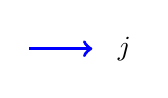
\begin{tikzpicture}[baseline=-0.5ex]
                        \draw[blue, very thick, ->] (0,0) -- (0.8,0);
                        \node[right=0.2cm] at (0.8,0) {$j$};
                    \end{tikzpicture}\\[0.4em]
                };

            \end{scope}
            \def\R{2.7}
            \def\r{0.7}
            \def\initialdeltaR{90}
            \def\initialdelta{-90}
            \def\msiz{4}
            \begin{scope}[>={Stealth[length=1.5mm, width=1.1mm]},shift={(0, 8)}]
                \coordinate (A1) at (\initialdeltaR:\R);
                \coordinate (A2) at (\initialdeltaR+120:\R);
                \coordinate (A3) at (\initialdeltaR-120:\R);
                \node at (-\R-0.2,\R+0.2) {$(1)$};

                % ================= 节点 =================
                \node[circle, draw=gray!50, fill=gray!2, minimum size=\msiz] (T01) at (\initialdeltaR:\r) {};
                \node[circle, draw=gray!50, fill=gray!2, minimum size=\msiz] (T02) at (\initialdeltaR+120:\r) {};
                \node[circle, draw=gray!50, fill=gray!2, minimum size=\msiz] (T03) at (\initialdeltaR-120:\r) {};
                \node[circle, draw=black, fill=gray!5, minimum size=\msiz] (T11) at ($(A1) + (\initialdelta:\r)$) {};
                \node[circle, draw=gray!50, fill=gray!2, minimum size=\msiz] (T12) at ($(A1) + (\initialdelta+120:\r)$) {};
                \node[circle, draw=gray!50, fill=gray!2, minimum size=\msiz] (T13) at ($(A1) + (\initialdelta-120:\r)$) {};
                \node[circle, draw=gray!50, fill=gray!2, minimum size=\msiz] (T21) at ($(A2) + (\initialdelta:\r)$) {};
                \node[circle, draw=gray!50, fill=gray!2, minimum size=\msiz] (T22) at ($(A2) + (\initialdelta+120:\r)$) {};
                \node[circle, draw=gray!50, fill=gray!2, minimum size=\msiz] (T23) at ($(A2) + (\initialdelta-120:\r)$) {};
                \node[circle, draw=black, fill=gray!5, minimum size=\msiz] (T31) at ($(A3) + (\initialdelta:\r)$) {};
                \node[circle, draw=gray!50, fill=gray!2, minimum size=\msiz] (T32) at ($(A3) + (\initialdelta+120:\r)$) {};
                \node[circle, draw=gray!50, fill=gray!2, minimum size=\msiz] (T33) at ($(A3) + (\initialdelta-120:\r)$) {};
            
                % ================= 箭头 =================
                \draw[->, blue, thick] (T01) -- (T02);  % tick
                \draw[->, blue, thick] (T02) -- (T03);  % tick
                \draw[->, blue!20, thick] (T03) -- (T01);
                \draw[->, blue, thick] (T11) -- (T12);  % tick
                \draw[->, blue, thick] (T12) -- (T13);  % tick
                \draw[->, blue!20, thick] (T13) -- (T11);
                \draw[->, blue!20, thick] (T21) -- (T22);
                \draw[->, blue!20, thick] (T22) -- (T23);
                \draw[->, blue, thick] (T23) -- (T21);  % tick
                \draw[->, blue!20, thick] (T31) -- (T32);
                \draw[->, blue!20, thick] (T32) -- (T33);
                \draw[->, blue, thick] (T33) -- (T31);  % tick
                \draw[<->, red, thick] (T01) -- (T11);  % tick
                \draw[<->, red!20, thick] (T02) -- (T22);
                \draw[<->, red, thick] (T03) -- (T33);  % tick
                \draw[<->, red, thick] (T13) -- (T23);  % tick
                \draw[<->, red, thick] (T21) -- (T31);  % tick
                \draw[<->, red!20, thick] (T12) -- (T32);
            \end{scope}
            \begin{scope}[>={Stealth[length=1.5mm, width=1.1mm]},shift={(7, 8)}]
                \coordinate (A1) at (\initialdeltaR:\R);
                \coordinate (A2) at (\initialdeltaR+120:\R);
                \coordinate (A3) at (\initialdeltaR-120:\R);
                \node at (-\R-0.2,\R+0.2) {$(2)$};

                % ================= 节点 =================
                \node[circle, draw=black, fill=gray!5, minimum size=\msiz] (T01) at (\initialdeltaR:\r) {};
                \node[circle, draw=gray!50, fill=gray!2, minimum size=\msiz] (T02) at (\initialdeltaR+120:\r) {};
                \node[circle, draw=gray!50, fill=gray!2, minimum size=\msiz] (T03) at (\initialdeltaR-120:\r) {};
                \node[circle, draw=gray!50, fill=gray!2, minimum size=\msiz] (T11) at ($(A1) + (\initialdelta:\r)$) {};
                \node[circle, draw=gray!50, fill=gray!2, minimum size=\msiz] (T12) at ($(A1) + (\initialdelta+120:\r)$) {};
                \node[circle, draw=gray!50, fill=gray!2, minimum size=\msiz] (T13) at ($(A1) + (\initialdelta-120:\r)$) {};
                \node[circle, draw=gray!50, fill=gray!2, minimum size=\msiz] (T21) at ($(A2) + (\initialdelta:\r)$) {};
                \node[circle, draw=gray!50, fill=gray!2, minimum size=\msiz] (T22) at ($(A2) + (\initialdelta+120:\r)$) {};
                \node[circle, draw=gray!50, fill=gray!2, minimum size=\msiz] (T23) at ($(A2) + (\initialdelta-120:\r)$) {};
                \node[circle, draw=gray!50, fill=gray!2, minimum size=\msiz] (T31) at ($(A3) + (\initialdelta:\r)$) {};
                \node[circle, draw=black, fill=gray!5,  minimum size=\msiz] (T32) at ($(A3) + (\initialdelta+120:\r)$) {};
                \node[circle, draw=gray!50, fill=gray!2, minimum size=\msiz] (T33) at ($(A3) + (\initialdelta-120:\r)$) {};
            
                % ================= 箭头 =================
                \draw[->, blue, thick] (T01) -- (T02);  % tick
                \draw[->, blue!20, thick] (T02) -- (T03);
                \draw[->, blue!20, thick] (T03) -- (T01);
                \draw[->, blue, thick] (T11) -- (T12);  % tick
                \draw[->, blue!20, thick] (T12) -- (T13);
                \draw[->, blue!20, thick] (T13) -- (T11);
                \draw[->, blue!20, thick] (T21) -- (T22);
                \draw[->, blue, thick] (T22) -- (T23);  % tick
                \draw[->, blue, thick] (T23) -- (T21);  % tick
                \draw[->, blue, thick] (T31) -- (T32);  % tick
                \draw[->, blue!20, thick] (T32) -- (T33);
                \draw[->, blue!20, thick] (T33) -- (T31);
                \draw[<->, red, thick] (T01) -- (T11);  % tick
                \draw[<->, red, thick] (T02) -- (T22);  % tick
                \draw[<->, red!20, thick] (T03) -- (T33);
                \draw[<->, red!20, thick] (T13) -- (T23);
                \draw[<->, red, thick] (T21) -- (T31);  % tick
                \draw[<->, red, thick] (T12) -- (T32);  % tick

            \end{scope}
            \begin{scope}[>={Stealth[length=1.5mm, width=1.1mm]},shift={(14,8)}]
                \coordinate (A1) at (\initialdeltaR:\R);
                \coordinate (A2) at (\initialdeltaR+120:\R);
                \coordinate (A3) at (\initialdeltaR-120:\R);
                \node at (-\R-0.2,\R+0.2) {$(3)$};

                % ================= 节点 =================
                \node[circle, draw=gray!50, fill=gray!2, minimum size=\msiz] (T01) at (\initialdeltaR:\r) {};
                \node[circle, draw=gray!50, fill=gray!2, minimum size=\msiz] (T02) at (\initialdeltaR+120:\r) {};
                \node[circle, draw=gray!50, fill=gray!2, minimum size=\msiz] (T03) at (\initialdeltaR-120:\r) {};
                \node[circle, draw=gray!50, fill=gray!2, minimum size=\msiz] (T11) at ($(A1) + (\initialdelta:\r)$) {};
                \node[circle, draw=gray!50, fill=gray!2, minimum size=\msiz] (T12) at ($(A1) + (\initialdelta+120:\r)$) {};
                \node[circle, draw=black, fill=gray!5, minimum size=\msiz] (T13) at ($(A1) + (\initialdelta-120:\r)$) {};
                \node[circle, draw=gray!50, fill=gray!2, minimum size=\msiz] (T21) at ($(A2) + (\initialdelta:\r)$) {};
                \node[circle, draw=gray!50, fill=gray!2, minimum size=\msiz] (T22) at ($(A2) + (\initialdelta+120:\r)$) {};
                \node[circle, draw=gray!50, fill=gray!2, minimum size=\msiz] (T23) at ($(A2) + (\initialdelta-120:\r)$) {};
                \node[circle, draw=gray!50, fill=gray!2, minimum size=\msiz] (T31) at ($(A3) + (\initialdelta:\r)$) {};
                \node[circle, draw=gray!50, fill=gray!2, minimum size=\msiz] (T32) at ($(A3) + (\initialdelta+120:\r)$) {};
                \node[circle, draw=black, fill=gray!5, minimum size=\msiz] (T33) at ($(A3) + (\initialdelta-120:\r)$) {};
            
                % ================= 箭头 =================
                \draw[->, blue!20, thick] (T01) -- (T02);
                \draw[->, blue, thick] (T02) -- (T03);  % tick
                \draw[->, blue!20, thick] (T03) -- (T01);
                \draw[->, blue, thick] (T11) -- (T12);  % tick
                \draw[->, blue!20, thick] (T12) -- (T13);
                \draw[->, blue, thick] (T13) -- (T11);  % tick
                \draw[->, blue, thick] (T21) -- (T22);  % tick
                \draw[->, blue!20, thick] (T22) -- (T23);
                \draw[->, blue, thick] (T23) -- (T21);  % tick
                \draw[->, blue!20, thick] (T31) -- (T32);
                \draw[->, blue, thick] (T32) -- (T33);  % tick
                \draw[->, blue!20, thick] (T33) -- (T31);
                \draw[<->, red!20, thick] (T01) -- (T11);
                \draw[<->, red, thick] (T02) -- (T22);  % tick
                \draw[<->, red, thick] (T03) -- (T33);  % tick
                \draw[<->, red, thick] (T13) -- (T23);  % tick
                \draw[<->, red!20, thick] (T21) -- (T31);
                \draw[<->, red, thick] (T12) -- (T32);  % tick

                % ================= 右侧图例 =================
                \node[font=\small, anchor=north west, align=left] at (3,3.5)
                {
                    \textbf{变换图例：}\\[0.5em]
                    \begin{tikzpicture}[baseline=-0.5ex]
                        \draw[red, thick, ->] (0,0) -- (0.8,0);
                        \node[right=0.2cm] at (0.8,0) {$a$};
                    \end{tikzpicture}\\[0.4em]
                    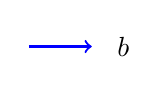
\begin{tikzpicture}[baseline=-0.5ex]
                        \draw[blue, thick, ->] (0,0) -- (0.8,0);
                        \node[right=0.2cm] at (0.8,0) {$b$};
                    \end{tikzpicture}\\[0.4em]
                };
            \end{scope}
        \end{tikzpicture}
        \label{fig:A_4-and-quaternion-group-cayley}
    \end{figure}
    \item 判断以下集合中的运算是否是交换的。
    \begin{problemlist}
        \item 整数集中的乘法运算。
        \item 有理数集中的减法运算。
        \item 实系数$3\times 3$矩阵的矩阵乘法运算。
        \item 模$p$非零同余类的乘法运算（$p$为素数）。
        \item 从$[\,0;1\,]$映射到$[\,0;1\,]$的连续函数集的复合运算。
    \end{problemlist}
    \item 如何写出整数加法群的乘法表？给出你的想法。
    \item 下图是一张没填完的群乘法表。怎样将它补完？补完的方式不止一种。分别讨论每种情况对应的群有什么特点。
    \vspace{12pt}
    \begin{table}[htbp]
        \centering
        \label{tab:4-multiplication-completion}
        \renewcommand{\arraystretch}{1} 
        \setlength{\tabcolsep}{7pt} 
        \begin{tabular}{|c|c!{\color{gray!50}\vrule}c!{\color{gray!50}\vrule}c!{\color{gray!50}\vrule}c|}
            \hline
            $\cdot$ & $e$ & $a$ & $b$ & $c$ \\
            \hline
            $e$     & & & & \\
            \arrayrulecolor{gray!50}
            \hline
            \arrayrulecolor{black}
            $a$     & & $e$ & & \\
            \arrayrulecolor{gray!50}
            \hline
            \arrayrulecolor{black}
            $b$     & & & & \\
            \arrayrulecolor{gray!50}
            \hline
            \arrayrulecolor{black}
            $c$     & & & & \\
            \hline
        \end{tabular}
    \end{table}
    \item 下图是五元循环群$\mathsf{C}_5$和四元数群$\mathsf{U}_4$的生成路径图。
    \vspace{12pt}
    \begin{figure}[htbp]
        \centering
        \begin{tikzpicture}[scale=0.7, thick]
            \begin{scope}[>={Latex[length=3mm,width=2mm]},shift={(0,0)}]
                \def\msiz{24}  % 节点最小半径
                \def\R{2.8}
                \def\initialtheta{90}
                \def\n{5}
                \def\abend{20}
                \node[circle, draw=black, fill=gray!5, minimum size=\msiz] (n0) at (\initialtheta-0*360/\n:\R) {};
                \node[circle, draw=black, fill=gray!5, minimum size=\msiz] (n1) at (\initialtheta-1*360/\n:\R) {};
                \node[circle, draw=black, fill=gray!5, minimum size=\msiz] (n2) at (\initialtheta-2*360/\n:\R) {};
                \node[circle, draw=black, fill=gray!5, minimum size=\msiz] (n3) at (\initialtheta-3*360/\n:\R) {};
                \node[circle, draw=black, fill=gray!5, minimum size=\msiz] (n4) at (\initialtheta-4*360/\n:\R) {};
                \node at (n0) {$e$};
                \node at (n1) {$a$};
                \node at (n2) {$a^2$};
                \node at (n3) {$a^3$};
                \node at (n4) {$a^4$};
                \draw[->, red, very thick, >=latex] (n0) to[bend left=\abend] (n1);
                \draw[->, red, very thick, >=latex] (n1) to[bend left=\abend] (n2);
                \draw[->, red, very thick, >=latex] (n2) to[bend left=\abend] (n3);
                \draw[->, red, very thick, >=latex] (n3) to[bend left=\abend] (n4);
                \draw[->, red, very thick, >=latex] (n4) to[bend left=\abend] (n0);
                % ================= 右侧图例 =================
                
                \node[font=\small, anchor=north west, align=left] at (3.6,2.6)
                {
                    \textbf{变换图例：}\\[0.5em]
                    \begin{tikzpicture}[baseline=-0.5ex]
                        \draw[red, thick, ->] (0,0) -- (0.8,0);
                        \node[right=0.2cm] at (0.8,0) {$a$};
                    \end{tikzpicture}\\[0.4em]
                };
            \end{scope}
            \begin{scope}[>=Stealth, shift={(11,0)}]  %  
                \def\msiz{24}  % 节点最小半径
                \def\R{2.7}  % 圆形半径
                \def\initialtheta{0.0}  % 初始角度

                % ================= 节点 =================
                \node[circle, draw=black, fill=gray!5, minimum size=\msiz] (A0) at (\initialtheta-0*45:\R) {$1$};
                \node[circle, draw=black, fill=gray!5, minimum size=\msiz] (A1) at (\initialtheta-1*45:\R) {$j$};
                \node[circle, draw=black, fill=gray!5, minimum size=\msiz] (A2) at (\initialtheta-2*45:\R) {};
                \node[circle, draw=black, fill=gray!5, minimum size=\msiz] (A3) at (\initialtheta-3*45:\R) {};
                \node[circle, draw=black, fill=gray!5, minimum size=\msiz] (A4) at (\initialtheta-4*45:\R) {};
                \node[circle, draw=black, fill=gray!5, minimum size=\msiz] (A5) at (\initialtheta-5*45:\R) {};
                \node[circle, draw=black, fill=gray!5, minimum size=\msiz] (A6) at (\initialtheta-6*45:\R) {$k$};
                \node[circle, draw=black, fill=gray!5, minimum size=\msiz] (A7) at (\initialtheta-7*45:\R) {$i$};
                \node at (A2) {$-k$};
                \node at (A3) {$-i$};
                \node at (A4) {$-1$};
                \node at (A5) {$-j$};

                % ================= 箭头 =================
                \draw[->, blue, very thick] (A0) -- (A1);
                \draw[->, blue, very thick] (A4) -- (A5);
                \draw[->, blue, very thick] (A6) -- (A7);
                \draw[->, red, very thick] (A7) -- (A4);
                \draw[->, blue, very thick] (A3) -- (A6);
                \draw[->, red, very thick] (A5) -- (A2);
                \draw[->, red, very thick] (A3) -- (A0);
                \draw[->, red, very thick] (A2) -- (A1);
                \draw[->, blue, very thick] (A2) -- (A3);  % tick
                \draw[->, blue, very thick] (A7) -- (A2);  % tick
                \draw[->, red, very thick] (A1) -- (A6);  % tick
                \draw[->, blue, very thick] (A5) -- (A0);  % tick
                \draw[->, blue, very thick] (A1) -- (A4);  % tick
                \draw[->, red, very thick] (A0) -- (A7);  % tick
                \draw[->, red, very thick] (A4) -- (A3);  % tick
                \draw[->, red, very thick] (A6) -- (A5);  % tick
            
                % ================= 右侧图例 =================
                
                \node[font=\small, anchor=north west, align=left] at (3.5,2.6)
                {
                    \textbf{变换图例：}\\[0.5em]
                    \begin{tikzpicture}[baseline=-0.5ex]
                        \draw[red, thick, ->] (0,0) -- (0.8,0);
                        \node[right=0.2cm] at (0.8,0) {$i$};
                    \end{tikzpicture}\\[0.4em]
                    \begin{tikzpicture}[baseline=-0.5ex]
                        \draw[blue, thick, ->] (0,0) -- (0.8,0);
                        \node[right=0.2cm] at (0.8,0) {$j$};
                    \end{tikzpicture}\\[0.4em]
                };

            \end{scope}
        \end{tikzpicture}
    \label{fig:C_5-and-quaternion-group-cayley}
    \end{figure}
    \begin{problemlist}
        \item $\mathsf{C}_5$中，$a^3$是什么变换？它如何改变图中的状态？
        \item $\mathsf{C}_5$中，$a^5$是什么变换？它如何改变图中的状态？
        \item $\mathsf{U}_4$中，$ij$和$ji$分别是什么变换？它如何改变图中的状态？
        \item $\mathsf{U}_4$中，$jji$是什么变换？它如何改变图中的状态？
        \item 写出两个群的乘法表。
    \end{problemlist}
\end{problemlist}

\subsection*{似群非群}

\begin{problemlist}
    \item 考虑以下二元运算的乘法表：
    \vspace{12pt}
    \begin{table}[htbp]
        \centering
        \label{tab:33-multiplication-nongroup1}
        \renewcommand{\arraystretch}{1} 
        \setlength{\tabcolsep}{7pt} 
        \begin{tabular}{|c|c!{\color{gray!50}\vrule}c!{\color{gray!50}\vrule}c!{\color{gray!50}\vrule}c|}
            \hline
            $\cdot$ & $e$ & $a$ & $b$ \\
            \hline
            $e$     & $e$ & $a$ & $b$ \\
            \arrayrulecolor{gray!50}
            \hline
            \arrayrulecolor{black}
            $a$     & $a$ & $e$ & $e$ \\
            \arrayrulecolor{gray!50}
            \hline
            \arrayrulecolor{black}
            $b$     & $b$ & $e$ & $e$\\
            \hline
        \end{tabular}
    \end{table}
    \begin{problemlist}
        \item 说明为什么这个二元运算不满足结合律（可以用式子表示）。
        \item 这个二元运算下，各个元素有逆元吗？为什么这么说？
    \end{problemlist}
    \item 考虑以下二元运算的乘法表：
    \vspace{12pt}
    \begin{table}[htbp]
        \centering
        \label{tab:33-multiplication-nongroup2}
        \renewcommand{\arraystretch}{1} 
        \setlength{\tabcolsep}{7pt} 
        \begin{tabular}{|c|c!{\color{gray!50}\vrule}c!{\color{gray!50}\vrule}c!{\color{gray!50}\vrule}c|}
            \hline
            $\cdot$ & $e$ & $a$ & $b$ \\
            \hline
            $e$     & $e$ & $a$ & $b$ \\
            \arrayrulecolor{gray!50}
            \hline
            \arrayrulecolor{black}
            $a$     & $a$ & $a$ & $b$ \\
            \arrayrulecolor{gray!50}
            \hline
            \arrayrulecolor{black}
            $b$     & $b$ & $b$ & $b$\\
            \hline
        \end{tabular}
    \end{table}
    \begin{problemlist}
        \item 说明这个二元运算满足结合律（可以用式子表示）。
        \item 这个二元运算下，各个元素有逆元吗？为什么这么说？
    \end{problemlist}
    \item 考虑以下二元运算的乘法表：
    \vspace{12pt}
    \begin{table}[htbp]
        \centering
        \label{tab:33-multiplication-nongroup3}
        \renewcommand{\arraystretch}{1} 
        \setlength{\tabcolsep}{7pt} 
        \begin{tabular}{|c|c!{\color{gray!50}\vrule}c!{\color{gray!50}\vrule}c!{\color{gray!50}\vrule}c|}
            \hline
            $\cdot$ & $e$ & $a$ & $b$ \\
            \hline
            $e$     & $e$ & $a$ & $b$ \\
            \arrayrulecolor{gray!50}
            \hline
            \arrayrulecolor{black}
            $a$     & $a$ & $b$ & $b$ \\
            \arrayrulecolor{gray!50}
            \hline
            \arrayrulecolor{black}
            $b$     & $b$ & $b$ & $b$\\
            \hline
        \end{tabular}
    \end{table}
    \begin{problemlist}
        \item 这个二元运算满足结合律吗？为什么这么说？
        \item 这个二元运算下，各个元素有逆元吗？为什么这么说？
    \end{problemlist}
    \item 解释以下的乘法表对应的运算为什么不构成群？
    \begin{center}
        \begin{minipage}{\textwidth}
            \noindent
            \renewcommand{\arraystretch}{1} 
            \setlength{\tabcolsep}{7pt} 
            \begin{minipage}[t]{0.48\textwidth}
                (1)
                \label{tab:44-multiplication-nongroup1}
                \hspace{4pt}
                % 没有幺元
                \begin{tabular}{|c|c!{\color{gray!50}\vrule}c!{\color{gray!50}\vrule}c!{\color{gray!50}\vrule}c|}
                    \hline
                    $\cdot$ & $e$ & $a$ & $b$ & $c$ \\
                    \hline
                    $e$     & $e$ & $a$ & $c$ & $b$ \\
                    \arrayrulecolor{gray!50}
                    \hline
                    \arrayrulecolor{black}
                    $a$     & $a$ & $b$ & $c$ & $e$ \\
                    \arrayrulecolor{gray!50}
                    \hline
                    \arrayrulecolor{black}
                    $b$     & $b$ & $c$ & $e$ & $a$ \\
                    \arrayrulecolor{gray!50}
                    \hline
                    \arrayrulecolor{black}
                    $c$     & $c$ & $e$ & $a$ & $b$ \\
                    \hline
                \end{tabular}
            \end{minipage}
            \hfill
            \begin{minipage}[t]{0.48\textwidth}
                (2)
                \label{tab:44-multiplication-nongroup2}
                \hspace{4pt}
                % e 是幺元
                % aa = a = ab, 所以 a = b，矛盾！
                \begin{tabular}{|c|c!{\color{gray!50}\vrule}c!{\color{gray!50}\vrule}c!{\color{gray!50}\vrule}c|}
                    \hline
                    $\cdot$ & $e$ & $a$ & $b$ & $c$ \\
                    \hline
                    $e$     & $e$ & $a$ & $b$ & $c$ \\
                    \arrayrulecolor{gray!50}
                    \hline
                    \arrayrulecolor{black}
                    $a$     & $a$ & $a$ & $b$ & $c$ \\
                    \arrayrulecolor{gray!50}
                    \hline
                    \arrayrulecolor{black}
                    $b$     & $b$ & $a$ & $b$ & $c$ \\
                    \arrayrulecolor{gray!50}
                    \hline
                    \arrayrulecolor{black}
                    $c$     & $c$ & $a$ & $b$ & $c$ \\
                    \hline
                \end{tabular}
            \end{minipage}

            \vspace{1em}

            \hspace{4pt}
            \begin{minipage}[t]{0.48\textwidth}
                (3)
                \label{tab:55-multiplication-nongroup1}
                \hspace{4pt}
                % e 是幺元
                % aa = c,  cc = d, dd = c, 因此 ccc = e,
                % dc = a = ccc = e。矛盾
                \begin{tabular}{|c|c!{\color{gray!50}\vrule}c!{\color{gray!50}\vrule}c!{\color{gray!50}\vrule}c!{\color{gray!50}\vrule}c|}
                    \hline
                    $\cdot$ & $e$ & $a$ & $b$ & $c$ & $d$ \\
                    \hline
                    $e$     & $e$ & $a$ & $b$ & $c$ & $d$ \\
                    \arrayrulecolor{gray!50}
                    \hline
                    \arrayrulecolor{black}
                    $a$     & $a$ & $c$ & $d$ & $e$ & $b$ \\
                    \arrayrulecolor{gray!50}
                    \hline
                    \arrayrulecolor{black}
                    $b$     & $b$ & $d$ & $c$ & $a$ & $e$ \\
                    \arrayrulecolor{gray!50}
                    \hline
                    \arrayrulecolor{black}
                    $c$     & $c$ & $b$ & $e$ & $d$ & $a$ \\
                    \arrayrulecolor{gray!50}
                    \hline
                    \arrayrulecolor{black}
                    $d$     & $d$ & $e$ & $a$ & $b$ & $c$ \\
                    \hline
                \end{tabular}
            \end{minipage}
            \hfill
            \begin{minipage}[t]{0.48\textwidth}
                (4)
                \label{tab:55-multiplication-nongroup2}
                \hspace{4pt}
                % e 是幺元
                % da = b, cb = a, 因此 cda = a, cd = e
                % 但 cd = b, 矛盾！
                \begin{tabular}{|c|c!{\color{gray!50}\vrule}c!{\color{gray!50}\vrule}c!{\color{gray!50}\vrule}c!{\color{gray!50}\vrule}c|}
                    \hline
                    $\cdot$ & $e$ & $a$ & $b$ & $c$ & $d$ \\
                    \hline
                    $e$     & $e$ & $a$ & $b$ & $c$ & $d$ \\
                    \arrayrulecolor{gray!50}
                    \hline
                    \arrayrulecolor{black}
                    $a$     & $a$ & $e$ & $c$ & $d$ & $b$ \\
                    \arrayrulecolor{gray!50}
                    \hline
                    \arrayrulecolor{black}
                    $b$     & $b$ & $d$ & $e$ & $a$ & $c$ \\
                    \arrayrulecolor{gray!50}
                    \hline
                    \arrayrulecolor{black}
                    $c$     & $c$ & $b$ & $d$ & $e$ & $a$ \\
                    \arrayrulecolor{gray!50}
                    \hline
                    \arrayrulecolor{black}
                    $d$     & $d$ & $c$ & $a$ & $b$ & $e$ \\
                    \hline
                \end{tabular}
            \end{minipage}
        \end{minipage}
    \end{center}
    \item 为什么说群的乘法表里，群的每个元素在每一行恰好出现一次？每一列是否也有这样的情况？
    \item 解释以下的图为什么不是群的生成路径图？
    \vspace{20pt}
    % (1). 依图有 aba = abba（从中心到圆周转一次或两次再回归中心）, 即b = e，矛盾！
    % (2). 依图有 aa = bb = ab（正右到正左，正上到正下），即a = b，矛盾！
    \begin{figure}[htbp]
        \centering
    \begin{tikzpicture}[scale=0.7, thick]
    \begin{scope}[>={Latex[length=3mm,width=2mm]},shift={(0,0)}]
        \def\msiz{24}  % 节点最小半径
        \def\R{2.8}
        \def\initialtheta{90}
        \def\n{5}
        \def\abend{20}
        \node[circle, draw=black, fill=gray!5, minimum size=\msiz] (C) at (0,0) {};
        \node[circle, draw=black, fill=gray!5, minimum size=\msiz] (n0) at (\initialtheta-0*360/\n:\R) {};
        \node[circle, draw=black, fill=gray!5, minimum size=\msiz] (n1) at (\initialtheta-1*360/\n:\R) {};
        \node[circle, draw=black, fill=gray!5, minimum size=\msiz] (n2) at (\initialtheta-2*360/\n:\R) {};
        \node[circle, draw=black, fill=gray!5, minimum size=\msiz] (n3) at (\initialtheta-3*360/\n:\R) {};
        \node[circle, draw=black, fill=gray!5, minimum size=\msiz] (n4) at (\initialtheta-4*360/\n:\R) {};
        \draw[->, blue, very thick, >=latex] (n0) to[bend left=\abend] (n1);
        \draw[->, blue, very thick, >=latex] (n1) to[bend left=\abend] (n2);
        \draw[->, blue, very thick, >=latex] (n2) to[bend left=\abend] (n3);
        \draw[->, blue, very thick, >=latex] (n3) to[bend left=\abend] (n4);
        \draw[->, blue, very thick, >=latex] (n4) to[bend left=\abend] (n0);
        \draw[<->, red, very thick, >=latex] (n0) -- (C);
        \draw[<->, red, very thick, >=latex] (n1) -- (C);
        \draw[<->, red, very thick, >=latex] (n2) -- (C);
        \draw[<->, red, very thick, >=latex] (n3) -- (C);
        \draw[<->, red, very thick, >=latex] (n4) -- (C);
        \node at (-\R-0.3,\R+0.3) {$(1)$};
        % ================= 右侧图例 =================
        
        \node[font=\small, anchor=north west, align=left] at (3.6,2.6)
        {
            \textbf{变换图例：}\\[0.5em]
            \begin{tikzpicture}[baseline=-0.5ex]
                \draw[red, thick, ->] (0,0) -- (0.8,0);
                \node[right=0.2cm] at (0.8,0) {$a$};
            \end{tikzpicture}\\[0.4em]
            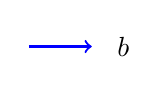
\begin{tikzpicture}[baseline=-0.5ex]
                \draw[blue, thick, ->] (0,0) -- (0.8,0);
                \node[right=0.2cm] at (0.8,0) {$b$};
            \end{tikzpicture}
        };
    \end{scope}
    \begin{scope}[>=Stealth, shift={(11,0)}]  %  
        \def\msiz{24}  % 节点最小半径
        \def\R{2.7}  % 圆形半径
        \def\initialtheta{0.0}  % 初始角度

        % ================= 节点 =================
        \node[circle, draw=black, fill=gray!5, minimum size=\msiz] (A0) at (\initialtheta-0*45:\R) {};
        \node[circle, draw=black, fill=gray!5, minimum size=\msiz] (A1) at (\initialtheta-1*45:\R) {};
        \node[circle, draw=black, fill=gray!5, minimum size=\msiz] (A2) at (\initialtheta-2*45:\R) {};
        \node[circle, draw=black, fill=gray!5, minimum size=\msiz] (A3) at (\initialtheta-3*45:\R) {};
        \node[circle, draw=black, fill=gray!5, minimum size=\msiz] (A4) at (\initialtheta-4*45:\R) {};
        \node[circle, draw=black, fill=gray!5, minimum size=\msiz] (A5) at (\initialtheta-5*45:\R) {};
        \node[circle, draw=black, fill=gray!5, minimum size=\msiz] (A6) at (\initialtheta-6*45:\R) {};
        \node[circle, draw=black, fill=gray!5, minimum size=\msiz] (A7) at (\initialtheta-7*45:\R) {};

        % ================= 箭头 =================
        \draw[->, blue, very thick] (A0) -- (A1);
        \draw[->, blue, very thick] (A4) -- (A5);
        \draw[->, blue, very thick] (A6) -- (A7);
        \draw[->, red, very thick] (A7) -- (A4);
        \draw[->, blue, very thick] (A3) -- (A6);
        \draw[->, blue, very thick] (A5) -- (A2);
        \draw[->, red, very thick] (A3) -- (A0);
        \draw[->, red, very thick] (A2) -- (A1);
        \draw[->, blue, very thick] (A2) -- (A3); 
        \draw[->, blue, very thick] (A7) -- (A2); 
        \draw[->, red, very thick] (A1) -- (A6); 
        \draw[->, red, very thick] (A5) -- (A0); 
        \draw[->, blue, very thick] (A1) -- (A4); 
        \draw[->, red, very thick] (A0) -- (A7); 
        \draw[->, red, very thick] (A4) -- (A3); 
        \draw[->, red, very thick] (A6) -- (A5); 
        \node at (-\R-0.3,\R+0.3) {$(2)$};
        % ================= 右侧图例 =================
        
        \node[font=\small, anchor=north west, align=left] at (3.5,2.6)
        {
            \textbf{变换图例：}\\[0.5em]
            \begin{tikzpicture}[baseline=-0.5ex]
                \draw[red, thick, ->] (0,0) -- (0.8,0);
                \node[right=0.2cm] at (0.8,0) {$a$};
            \end{tikzpicture}\\[0.4em]
            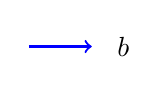
\begin{tikzpicture}[baseline=-0.5ex]
                \draw[blue, thick, ->] (0,0) -- (0.8,0);
                \node[right=0.2cm] at (0.8,0) {$b$};
            \end{tikzpicture}\\[0.4em]
        };

    \end{scope}
    \end{tikzpicture}
    \label{fig:C_6-and-quaternion-group-faux-cayley}
    \end{figure}
\end{problemlist}

\subsection*{群的代数定义}

\begin{problemlist}
    \item 验证以下的集合是否关于提到的运算构成群。
    \begin{problemlist}
        \item 所有$3$的倍数关于整数的加法。
        \item 所有$3$的倍数关于整数的乘法。
        \item 非零实数关于乘方。
        \item 所有完全平方数关于整数的乘法。
        \item 所有非零的完全平方有理数关于有理数的乘法。完全平方有理数指能够写成两个完全平方数相除的商的数。
        \item 所有素数有理数关于有理数的乘法。素数有理数指能写成两个素数商的数。
        \item 模$n$的简化同余系关于同余类的乘法。简化同余系指与$n$互素的同余类的集合。
        \item 由$2$和$3$不断相乘、相除、取相反数得到的所有数的集合：$\{\pm 2^n3^m\,|\,n,m\in\mathbb{Z}\}$，关于有理数的乘法。
        \item 分母为完全平方数的非零有理数的集合，关于有理数的乘法。
    \end{problemlist}
    \item 验证以下的集合是否关于提到的运算构成群。
    \begin{problemlist}
        \item 整系数一元整式的集合$\mathbb{Z}[X]$关于整式的加法。
        \item 实系数一元整式的集合$\mathbb{R}[X]$关于整式的加法。
        \item 整系数一元整式的集合$\mathbb{Z}[X]$关于整式的乘法。
        \item 实系数一元整式的集合$\mathbb{R}[X]$关于整式的乘法。
        \item 实系数一元有理式的集合$\mathbb{R}(X)$关于整式的乘法。其中$\mathbb{R}(X)$是所有能表示为一元整式除以非零一元整式形式的式子的集合：
        \[ \mathbb{R}(X) = \left\{\frac{P(X)}{Q(X)}\,\bigg|\,P,Q\in\mathbb{R}[X],Q\neq0\right\}
        \]
        \item 偶系数一元整式的集合$\mathbb{B}[X]$关于整式的加法。其中$\mathbb{B}=\{2n\,\mid\,n\in\mathbb{Z}\}$。
        \item 奇系数一元整式的集合$\mathbb{J}[X]$关于整式的加法。其中$\mathbb{J}=\{2n+1\,\mid\,n\in\mathbb{Z}\}$。
    \end{problemlist}
    \item 考虑一个二元群$\{e,a\}$，其中$e$是幺元。
    \begin{problemlist}
        \item 证明：$aa=e$。
        \item 写出二元群$\{e,a\}$的乘法表。证明：二元群只有一种。
    \end{problemlist}
    \item 考虑一个三元群$\{e,a,b\}$，其中$e$是幺元。
    \begin{problemlist}
        \item 证明：$ab = e$。
        \item 用反证法证明：$aa\neq e$。
        \item 写出三元群$\{e,a,b\}$的乘法表。证明：三元群只有一种。
    \end{problemlist}
    \item 根据五元循环群$\mathsf{C}_5$和四元数群$\mathsf{U}_4$的生成路径图，给出群里每个元素的逆元素。用乘法表的话，如何找到逆元素？
\end{problemlist}

\chapter{四种常见的群}

上一章我们学习了群的正式定义，现在我们来了解四种常见的群。它们来自日常生活和生产中的种种现象和规律，反映了自然界和社会运行中对称性的体现和作用。

第一种群是循环群。循环群不仅是最简单的群结构，也是非常常见的一类。它不仅在生活中出现，也出现在更复杂的群里，是理解群的重要基础。循环群对应着群论中“环道”的概念，对我们理解接下来介绍的交换群和映轮群十分有帮助。最后我们会介绍置换群。置换群揭示了群和排列组合的关系，将为我们理解对称性提供非常关键的帮助。

本章的四种群不但会帮助你理解群的基本性质，而且会为你以后深入学习群论时提供丰富的例子，把抽象的思考过程变成直观的变换。请准备好在你的头脑里建设一个“群的博物馆”，将你即将见识的各种各样的群分门别类地存放在你的记忆中。它们的图像会在你以后遇到相关问题时生动地浮现出来。

\section{循环群}

回忆我们前几章提到的正三角形的对称变换群。里面包含了$6$个变换。其中$r_1$把正三角形逆时针旋转$120^\circ$。我们注意到，$r_1$重复三次后，就回到初始状态。在生成路径图中，$r_1$构成了一个三元循环。

讨论矩群时，我们用“向右转”对应的$4$元群来和它对比。里面的“向右转”重复$4$次后回到初始状态。如果我们把它的生成路径图画出来，就是一个$4$元循环。

\vspace{8pt}
\begin{figure}[htbp]
    \centering
    \begin{tikzpicture}[>=Stealth, thick, font=\normalsize]

        % ================= 节点与状态 =================
        \def\R{1.6} % 六边形半径
        
        % 绘制 6 个状态节点        
        % A1 (正上方, 90度)
        \pic[scale=0.8] (A1) at (90:\R) {tri={BrickRed}{LimeGreen}{RoyalBlue}};
        \node at (A1-C) {$A_1$};
        
        % A5 (左下, -150度)
        \pic[scale=0.8] (A2) at (-150:\R) {tri={RoyalBlue}{BrickRed}{LimeGreen}};
        \node at (A2-C) {$A_2$};
        
        % A3 (右下, -30度)
        \pic[scale=0.8] (A3) at (-30:\R) {tri={LimeGreen}{RoyalBlue}{BrickRed}};
        \node at (A3-C) {$A_3$};
        % 2. r1 (逆时针120度): 红色单向弧线
        \draw[Red, ->, thick, shorten <=15pt, shorten >=15pt] (A1-C) to (A2-C);
        \draw[Red, ->, thick, shorten <=15pt, shorten >=15pt] (A2-C) to (A3-C);
        \draw[Red, ->, thick, shorten <=15pt, shorten >=15pt] (A3-C) to (A1-C);
        % 循环群：C_4
        \begin{scope}[shift={(5,0.6)}, scale=0.8]
            \def\R{2.0}
            \def\initialtheta{90}
            \def\n{4}
            \def\abend{25}
            \node[circle, draw=black, minimum size=30] (n0) at (\initialtheta-0*360/\n:2) {};
            \node[circle, draw=black, minimum size=30] (n1) at (\initialtheta-1*360/\n:2) {};
            \node[circle, draw=black, minimum size=30] (n2) at (\initialtheta-2*360/\n:2) {};
            \node[circle, draw=black, minimum size=30] (n3) at (\initialtheta-3*360/\n:2) {};
            \draw[-{Latex[length=3mm,width=2mm]}, red, very thick, >=latex] (n0) to[bend left=\abend] (n1);
            \draw[-{Latex[length=3mm,width=2mm]}, red, very thick, >=latex] (n1) to[bend left=\abend] (n2);
            \draw[-{Latex[length=3mm,width=2mm]}, red, very thick, >=latex] (n2) to[bend left=\abend] (n3);
            \draw[-{Latex[length=3mm,width=2mm]}, red, very thick, >=latex] (n3) to[bend left=\abend] (n0);
            \filldraw[gray] (n0) ellipse (8pt and 3pt);
            \filldraw (n0) ++ (0, 0.1) circle (4pt);
            \filldraw[gray] (n1) ellipse (3pt and 8pt);
            \filldraw (n1) ++ (0.1, 0) circle (4pt);
            \filldraw[gray] (n2) ellipse (8pt and 3pt);
            \filldraw (n2) ++ (0, -0.1) circle (4pt);
            \filldraw[gray] (n3) ellipse (3pt and 8pt);
            \filldraw (n3) ++ (-0.1, 0) circle (4pt);
        \end{scope}
        
    \end{tikzpicture}
    \caption{\texttt{三元循环和四元循环}}
    \label{fig:three_four_cycles}
\end{figure}

这种由单个变换不断重复得到循环的现象，对应的群叫做\textbf{循环群}。循环群常常由旋转变换得到，揭示旋转、轮转的对称性质。上面两个例子都是关于旋转的变换。此外还有风车、螺旋桨、车轮等等。

一般来说，$n$元循环群就是有$n$个元素的循环群。具体来说，某个变换$a$出发，不断重复，得到新的变换。直到某次得到恒等变换$e$，把次数记为$n$。那么$a, a^2, \cdots, a^n=e$就构成一个$n$元循环群。$a$称为这个循环群的\textbf{生成元}。我们一般把$n$元循环群记作$\mathsf{C}_n$：
$$ \mathsf{C}_n = \{e, a, a^2, \cdots, a^{n-1}\}.$$
注意我们写到$a^{n-1}$为止，因为$a^n = e$在一开始已经写过了。

以上说法也许让你感到疑惑。首先，从变换$a$出发，不断重复，就一定能得到恒等变换$e$吗？答案是未必。但如果能得到，那么首次得到$e$的次数，就是$a$生成的循环群的大小。之前每一次重复，得到的都是新变换，和之前的变换都不一样。

这是为什么呢？让我们反过来思考。如果不断重复变换$a$时，某次出现的变换$a^j$和之前某个变换$a^i$一样：
$$ 0 < i < j, \,\;\; a^j = a^i.$$
其中$i,j$是正整数。考虑$a^{j-i}$，它表示做了$a^j$变换后，逆向做$i$次$a$变换得到的结果。但$a^j = a^i$，所以结果应该就是回到原状态，所以$a^{j-i} = e$。但由于$i$是正整数，$j-i<j$。也就是说，在得到$a^j$之前，我们必然已经得到了$a^{j-i} = e$。这就证明：$e$必然在任何重复出现的变换之前出现。得到$e$之前，不会有变换出现两次。$a,a^2,\cdots, a^n=e$中任何两个元素都不一样。这说明
$$ \mathsf{C}_n = \{e, a, a^2, \cdots, a^{n-1}\}$$
里确实有$n$个元素。

以下是$n$元循环群的生成路径图：

\vspace{12pt}
\begin{figure}[htbp]
    \centering
    \begin{tikzpicture}
        % 循环群：C_3
        \begin{scope}
            \def\R{2.0}
            \def\initialtheta{90}
            \def\n{3}
            \def\abend{40}
            \node[circle, draw=black, fill=gray!20, minimum size=30] (n0) at (\initialtheta-0*360/\n:2) {0};
            \node[circle, draw=black, fill=gray!20, minimum size=30] (n1) at (\initialtheta-1*360/\n:2) {1};
            \node[circle, draw=black, fill=gray!20, minimum size=30] (n2) at (\initialtheta-2*360/\n:2) {2};
            \draw[-{Latex[length=3mm,width=2mm]}, red, very thick, >=latex] (n0) to[bend left=\abend] (n1);
            \draw[-{Latex[length=3mm,width=2mm]}, red, very thick, >=latex] (n1) to[bend left=\abend] (n2);
            \draw[-{Latex[length=3mm,width=2mm]}, red, very thick, >=latex] (n2) to[bend left=\abend] (n0);
            \node[font=\Large] at (0,0) {\Large {$\mathsf{C}_{3}$}};
        \end{scope}
        % 循环群：C_5
        \begin{scope}[shift={(5,0)}]
            \def\R{2.0}
            \def\initialtheta{18}
            \def\n{5}
            \def\abend{20}
            \node[circle, draw=black, fill=gray!20, minimum size=1cm] (n0) at (\initialtheta-0*360/\n:2) {0};
            \node[circle, draw=black, fill=gray!20, minimum size=1cm] (n1) at (\initialtheta-1*360/\n:2) {1};
            \node[circle, draw=black, fill=gray!20, minimum size=1cm] (n2) at (\initialtheta-2*360/\n:2) {2};
            \node[circle, draw=black, fill=gray!20, minimum size=1cm] (n3) at (\initialtheta-3*360/\n:2) {3};
            \node[circle, draw=black, fill=gray!20, minimum size=1cm] (n4) at (\initialtheta-4*360/\n:2) {4};
            \draw[-{Latex[length=3mm,width=2mm]}, red, very thick, >=latex] (n0) to[bend left=\abend] (n1);
            \draw[-{Latex[length=3mm,width=2mm]}, red, very thick, >=latex] (n1) to[bend left=\abend] (n2);
            \draw[-{Latex[length=3mm,width=2mm]}, red, very thick, >=latex] (n2) to[bend left=\abend] (n3);
            \draw[-{Latex[length=3mm,width=2mm]}, red, very thick, >=latex] (n3) to[bend left=\abend] (n4);
            \draw[-{Latex[length=3mm,width=2mm]}, red, very thick, >=latex] (n4) to[bend left=\abend] (n0);
            \node[font=\Large] at (0,0) {\Large {$\mathsf{C}_{5}$}};
        \end{scope}
        % 循环群：\mathsf{C}_n
        \begin{scope}[shift={(10,0)}]
            \def\R{2.0}
            \def\initialtheta{90}
            \def\n{7}
            \def\abend{15}
            \node[circle, draw=black, fill=gray!20, minimum size=0.8cm] (n0) at (\initialtheta-0*360/\n:2) {0};
            \node[circle, draw=black, fill=gray!20, minimum size=0.8cm] (n1) at (\initialtheta-1*360/\n:2) {1};
            \node[circle, draw=black, fill=gray!20, minimum size=0.8cm] (n2) at (\initialtheta-2*360/\n:2) {2};
            \node[circle, draw=black, fill=gray!20, minimum size=0.8cm] (n6) at (\initialtheta+1*360/\n:2) {};
            \node[circle, draw=black, fill=gray!20, minimum size=0.8cm] (n5) at (\initialtheta+2*360/\n:2) {};
            \node[circle, draw=white, minimum size=0.8cm] (n3) at (\initialtheta-3*360/\n:2) {};
            \node[circle, draw=white, minimum size=0.8cm] (n4) at (\initialtheta+3*360/\n:2) {};
            \draw[-{Latex[length=3mm,width=2mm]}, red, very thick, >=latex] (n0) to[bend left=\abend] (n1);
            \draw[-{Latex[length=3mm,width=2mm]}, red, very thick, >=latex] (n1) to[bend left=\abend] (n2);
            \draw[-{Latex[length=3mm,width=2mm]}, red, very thick, >=latex] (n2) to[bend left=\abend] (n3);
            \draw[-{Latex[length=3mm,width=2mm]}, red, very thick, >=latex] (n4) to[bend left=\abend] (n5);
            \draw[-{Latex[length=3mm,width=2mm]}, red, very thick, >=latex] (n5) to[bend left=\abend] (n6);
            \draw[-{Latex[length=3mm,width=2mm]}, red, very thick, >=latex] (n6) to[bend left=\abend] (n0);
            \filldraw (0,0.05*\R) ++ (-70:\R) circle (1.2pt);
            \filldraw (0,0.05*\R) ++ (-90:\R) circle (1.2pt);
            \filldraw (0,0.05*\R) ++ (-110:\R) circle (1.2pt);
            \node[font=\Large] at (0,0) {\Large {$\mathsf{C}_{n}$}};
            \node at (n5) {\small {$n\!-\!2$}};
            \node at (n6) {\small {$n\!-\!1$}};
        \end{scope}
    \end{tikzpicture}
    \caption{\texttt{$3$元、$5$元乃至$n$元循环群}}
\end{figure}

循环群的生成路径图是一个圈。沿着走一圈就遍历了所有的元素。我们通常把$n$元循环群中的元素顺次记为$0,1,\cdots, n-1$。从$0$出发，第$1$个元素记为$1$，第二个元素记为$2$等等，最后一个元素记为$n-1$。这是因为模$n$的同余类$\{\overline{0},\overline{1},\cdots, \overline{n-1}\}$关于加法构成一个循环群：从$\overline{1}$开始不断加$\overline{1}$，就能得到所有$n$个同余类。

考察循环群里各号元素的关系，还可以用上一章引入的乘法表。当然，如果我们选择用$0$到$n-1$来编号的话，这个表应该叫做加法表。下面是$n=5$和$n=12$时的例子：

\newlength{\colwidth}
\setlength{\colwidth}{0.37cm} % 这里可以整体调控列宽
\renewcommand{\arraystretch}{1.2} % 这里可以整体调控行高

% 定义8种彩虹色基础颜色（0-7），8-11循环使用前四种
\definecolor{c0}{RGB}{255, 128, 128} % 0: 红
\definecolor{c1}{RGB}{255, 194, 102} % 1: 橙
\definecolor{c2}{RGB}{255, 255, 102} % 2: 黄
\definecolor{c3}{RGB}{138, 255, 138} % 3: 绿
\definecolor{c4}{RGB}{128, 255, 255} % 4: 青
\definecolor{c5}{RGB}{128, 160, 255} % 5: 蓝
\definecolor{c6}{RGB}{190, 128, 255} % 6: 紫
\definecolor{c7}{RGB}{255, 128, 255} % 7: 紫红

\begin{figure}[htbp]
    \centering
    \begin{tabular}{@{}c@{\hspace{4pt}}c@{}}

        % 【左侧部分】左上角占位 + 左侧表头
        \begin{tabular}{@{}c@{}}
            \vphantom{0} \\[6pt] % 透明的占位符，高度和数字0一样，正好对齐右侧的顶部行
            \begin{tabular}{|>{\centering\arraybackslash}p{\colwidth}|}
                \hline
                \cellcolor{c0}0 \\ \hline
                \cellcolor{c2}1 \\ \hline
                \cellcolor{c3}2 \\ \hline
                \cellcolor{c4}3 \\ \hline
                \cellcolor{c6}4 \\ \hline
            \end{tabular}
        \end{tabular}
        &
        % 【右侧部分】顶部表头 + 主体表格
        \begin{tabular}{@{}c@{}}
            \begin{tabular}{|>{\centering\arraybackslash}p{\colwidth}|>{\centering\arraybackslash}p{\colwidth}|>{\centering\arraybackslash}p{\colwidth}|>{\centering\arraybackslash}p{\colwidth}|>{\centering\arraybackslash}p{\colwidth}|}
                \hline
                \cellcolor{c0}0 & \cellcolor{c2}1 & \cellcolor{c3}2 & \cellcolor{c4}3 & \cellcolor{c6}4 \\ \hline
            \end{tabular} \\[6pt] % 用 \\[4pt] 制造出顶部和主体之间的垂直断开空隙
            \begin{tabular}{|>{\centering\arraybackslash}p{\colwidth}|>{\centering\arraybackslash}p{\colwidth}|>{\centering\arraybackslash}p{\colwidth}|>{\centering\arraybackslash}p{\colwidth}|>{\centering\arraybackslash}p{\colwidth}|}
                \hline
                \cellcolor{c0}0 & \cellcolor{c2}1 & \cellcolor{c3}2 & \cellcolor{c4}3 & \cellcolor{c6}4 \\ \hline
                \cellcolor{c2}1 & \cellcolor{c3}2 & \cellcolor{c4}3 & \cellcolor{c6}4 & \cellcolor{c0}0 \\ \hline
            \cellcolor{c3}2 & \cellcolor{c4}3 & \cellcolor{c6}4 & \cellcolor{c0}0 & \cellcolor{c2}1 \\ \hline
                \cellcolor{c4}3 & \cellcolor{c6}4 & \cellcolor{c0}0 & \cellcolor{c2}1 & \cellcolor{c3}2 \\ \hline
                \cellcolor{c6}4 & \cellcolor{c0}0 & \cellcolor{c2}1 & \cellcolor{c3}2 & \cellcolor{c4}3 \\ \hline
            \end{tabular}
        \end{tabular}

    \end{tabular}
    \caption{\texttt{$5$元循环群的加法表}}
\end{figure}

我们把相同的数用同样颜色的方格表示，可以发现循环群的加法表有美妙的规律。从右上到左下的各条对角线上总有相同的数值，因而有相同的颜色。我们用彩虹的颜色给从小到大的数逐个配色，就能得到彩虹一般的视觉效果。这个规律也很好解释，它让我们联想到平面直角坐标系上的直线：
$$ x + y = n.$$
它和水平线成$45$度角。要注意这里我们的“竖轴”是往下的。

\begin{figure}[t]
    \centering
    \begin{tabular}{@{}c@{\hspace{4pt}}c@{}}

        % 【左侧部分】左上角占位 + 左侧表头
        \begin{tabular}{@{}c@{}}
            \vphantom{0} \\[6pt] % 透明的占位符，高度和数字0一样，正好对齐右侧的顶部行
            \begin{tabular}{|>{\centering\arraybackslash}p{\colwidth}|}
                \hline
                \cellcolor{c0}0 \\ \hline
                \cellcolor{c1}1 \\ \hline
                \cellcolor{c2}2 \\ \hline
                \cellcolor{c3}3 \\ \hline
                \cellcolor{c4}4 \\ \hline
                \cellcolor{c5}5 \\ \hline
                \cellcolor{c6}6 \\ \hline
                \cellcolor{c7}7 \\ \hline
                \cellcolor{c0}8 \\ \hline
                \cellcolor{c1}9 \\ \hline
                \cellcolor{c2}10 \\ \hline
                \cellcolor{c3}11 \\ \hline
            \end{tabular}
        \end{tabular}
        &
        % 【右侧部分】顶部表头 + 主体表格
        \begin{tabular}{@{}c@{}}
            \begin{tabular}{|>{\centering\arraybackslash}p{\colwidth}|>{\centering\arraybackslash}p{\colwidth}|>{\centering\arraybackslash}p{\colwidth}|>{\centering\arraybackslash}p{\colwidth}|>{\centering\arraybackslash}p{\colwidth}|>{\centering\arraybackslash}p{\colwidth}|>{\centering\arraybackslash}p{\colwidth}|>{\centering\arraybackslash}p{\colwidth}|>{\centering\arraybackslash}p{\colwidth}|>{\centering\arraybackslash}p{\colwidth}|>{\centering\arraybackslash}p{\colwidth}|>{\centering\arraybackslash}p{\colwidth}|}
                \hline
                \cellcolor{c0}0 &
                \cellcolor{c1}1 &
                \cellcolor{c2}2 &
                \cellcolor{c3}3 &
                \cellcolor{c4}4 &
                \cellcolor{c5}5 &
                \cellcolor{c6}6 &
                \cellcolor{c7}7 &
                \cellcolor{c0}8 &
                \cellcolor{c1}9 &
                \cellcolor{c2}10 &
                \cellcolor{c3}11
                \\ \hline
            \end{tabular} \\[6pt] % 用 \\[4pt] 制造出顶部和主体之间的垂直断开空隙
            \begin{tabular}{|>{\centering\arraybackslash}p{\colwidth}|>{\centering\arraybackslash}p{\colwidth}|>{\centering\arraybackslash}p{\colwidth}|>{\centering\arraybackslash}p{\colwidth}|>{\centering\arraybackslash}p{\colwidth}|>{\centering\arraybackslash}p{\colwidth}|>{\centering\arraybackslash}p{\colwidth}|>{\centering\arraybackslash}p{\colwidth}|>{\centering\arraybackslash}p{\colwidth}|>{\centering\arraybackslash}p{\colwidth}|>{\centering\arraybackslash}p{\colwidth}|>{\centering\arraybackslash}p{\colwidth}|}
                \hline
                % 行0
                \cellcolor{c0}0 & \cellcolor{c1}1 & \cellcolor{c2}2 & \cellcolor{c3}3 & \cellcolor{c4}4 & \cellcolor{c5}5 & \cellcolor{c6}6 & \cellcolor{c7}7 & \cellcolor{c0}8 & \cellcolor{c1}9 & \cellcolor{c2}10 & \cellcolor{c3}11 \\ \hline

                % 行1
                \cellcolor{c1}1 & \cellcolor{c2}2 & \cellcolor{c3}3 & \cellcolor{c4}4 & \cellcolor{c5}5 & \cellcolor{c6}6 & \cellcolor{c7}7 & \cellcolor{c0}8 & \cellcolor{c1}9 & \cellcolor{c2}10 & \cellcolor{c3}11 & \cellcolor{c4}0 \\ \hline

                % 行2
                \cellcolor{c2}2 & \cellcolor{c3}3 & \cellcolor{c4}4 & \cellcolor{c5}5 & \cellcolor{c6}6 & \cellcolor{c7}7 & \cellcolor{c0}8 & \cellcolor{c1}9 & \cellcolor{c2}10 & \cellcolor{c3}11 & \cellcolor{c4}0 & \cellcolor{c5}1 \\ \hline

                % 行3
                \cellcolor{c3}3 & \cellcolor{c4}4 & \cellcolor{c5}5 & \cellcolor{c6}6 & \cellcolor{c7}7 & \cellcolor{c0}8 & \cellcolor{c1}9 & \cellcolor{c2}10 & \cellcolor{c3}11 & \cellcolor{c4}0 & \cellcolor{c5}1 & \cellcolor{c6}2 \\ \hline

                % 行4
                \cellcolor{c4}4 & \cellcolor{c5}5 & \cellcolor{c6}6 & \cellcolor{c7}7 & \cellcolor{c0}8 & \cellcolor{c1}9 & \cellcolor{c2}10 & \cellcolor{c3}11 & \cellcolor{c4}0 & \cellcolor{c5}1 & \cellcolor{c6}2 & \cellcolor{c7}3 \\ \hline

                % 行5
                \cellcolor{c5}5 & \cellcolor{c6}6 & \cellcolor{c7}7 & \cellcolor{c0}8 & \cellcolor{c1}9 & \cellcolor{c2}10 & \cellcolor{c3}11 & \cellcolor{c4}0 & \cellcolor{c5}1 & \cellcolor{c6}2 & \cellcolor{c7}3 & \cellcolor{c0}4 \\ \hline

                % 行6
                \cellcolor{c6}6 & \cellcolor{c7}7 & \cellcolor{c0}8 & \cellcolor{c1}9 & \cellcolor{c2}10 & \cellcolor{c3}11 & \cellcolor{c4}0 & \cellcolor{c5}1 & \cellcolor{c6}2 & \cellcolor{c7}3 & \cellcolor{c0}4 & \cellcolor{c1}5 \\ \hline

                % 行7
                \cellcolor{c7}7 & \cellcolor{c0}8 & \cellcolor{c1}9 & \cellcolor{c2}10 & \cellcolor{c3}11 & \cellcolor{c4}0 & \cellcolor{c5}1 & \cellcolor{c6}2 & \cellcolor{c7}3 & \cellcolor{c0}4 & \cellcolor{c1}5 & \cellcolor{c2}6 \\ \hline

                % 行8
                \cellcolor{c0}8 & \cellcolor{c1}9 & \cellcolor{c2}10 & \cellcolor{c3}11 & \cellcolor{c4}0 & \cellcolor{c5}1 & \cellcolor{c6}2 & \cellcolor{c7}3 & \cellcolor{c0}4 & \cellcolor{c1}5 & \cellcolor{c2}6 & \cellcolor{c3}7 \\ \hline

                % 行9
                \cellcolor{c1}9 & \cellcolor{c2}10 & \cellcolor{c3}11 & \cellcolor{c4}0 & \cellcolor{c5}1 & \cellcolor{c6}2 & \cellcolor{c7}3 & \cellcolor{c0}4 & \cellcolor{c1}5 & \cellcolor{c2}6 & \cellcolor{c3}7 & \cellcolor{c4}8 \\ \hline

                % 行10
                \cellcolor{c2}10 & \cellcolor{c3}11 & \cellcolor{c4}0 & \cellcolor{c5}1 & \cellcolor{c6}2 & \cellcolor{c7}3 & \cellcolor{c0}4 & \cellcolor{c1}5 & \cellcolor{c2}6 & \cellcolor{c3}7 & \cellcolor{c4}8 & \cellcolor{c5}9 \\ \hline

                % 行11
                \cellcolor{c3}11 & \cellcolor{c4}0 & \cellcolor{c5}1 & \cellcolor{c6}2 & \cellcolor{c7}3 & \cellcolor{c0}4 & \cellcolor{c1}5 & \cellcolor{c2}6 & \cellcolor{c3}7 & \cellcolor{c4}8 & \cellcolor{c5}9 & \cellcolor{c6}10 \\ \hline
            \end{tabular}
    \end{tabular}

    \end{tabular}
    \caption{\texttt{$12$元循环群的加法表}}
\end{figure}

最后，我们讨论“永远得不到$e$”的情况。也就是说，从群中某个变换$a$出发，不断重复，但得到的序列
$$ a, a^2, a^3, \cdots, a^n, a^{n+1}, \cdots $$
里没有$e$。这种情况下，这个序列里的变换两两不同。因为我们已经证明了：如果有$a^i = a^j$，就会出现$e$。因此，群的元素个数是无限的。此外，考虑$a$的逆元$a^{-1}$，它不断重复的结果也是两两不相同的序列：
$$ a^{-1}, a^{-2}, a^{-3}, \cdots, a^{-n}, a^{-n-1}, \cdots$$
其中$a^{-n}$就是$a^{-1}$重复$n$次的结果：$a^{-n} = \left(a^{-1}\right)^n$。

把以上两个序列和$e$合并，写成集合：
$$ \mathsf{C}_a = \{a^n\,\mid\,n\in\mathbb{Z}\}.$$
可以验证：这个集合是一个群。它有无限多个元素。我们把$\mathsf{C}_a$叫做变换$a$生成的\textbf{无限循环群}。即便它并没有真的“循环”，可它和循环群一样，都是靠$a$（及其逆变换）不断重复得来的。之后我们会看到，它确实和循环群有很多共同点，足以被归为一类。

\subsection{环道}

循环群不仅简单，而且是研究其他群的基础。任何群里总“隐藏”着循环群。比如我们研究过的三元对称群$\mathsf{D}_3$中，就包含了三元循环群。实际上，从任意群里找一个不是幺元的元素$a$，不断重复它，要么会在某个时刻得到$e$，要么永远得不到$e$。如果在第$n$次重复时首次得到$e$，就说明我们找到了$a$生成的$n$元循环群。如果永远得不到$e$，就说明我们找到了$a$生成的无限循环群。于是任何群里总有一部分是循环群。$a$生成的这个循环群称为$a$的\textbf{环道}。$a$生成的循环群的元素个数，叫做环道的长度或$a$的\textbf{阶}。

三元对称群$\mathsf{D}_3$的例子里，变换$r_1$构成一个长度为$3$的环道：$\{r_1, r_1^2, r_1^3 = e\}$。$r_2$也构成长度为$3$的环道：$\{r_2, r_2^2, r_2^3 = e\}$。$s_1,s_2,s_3$则各自属于一个长度为$2$的环道。由于$r_2 = r_1^2$，所以$r_2$的环道其实就是$r_1$的环道。$s_1,s_2,s_3$各自的环道则与$r_1,r_2$的环道不一样，只有$e$是共同元素。

% 插图：列举D_3的环道
\begin{figure}[htbp]
    \centering
    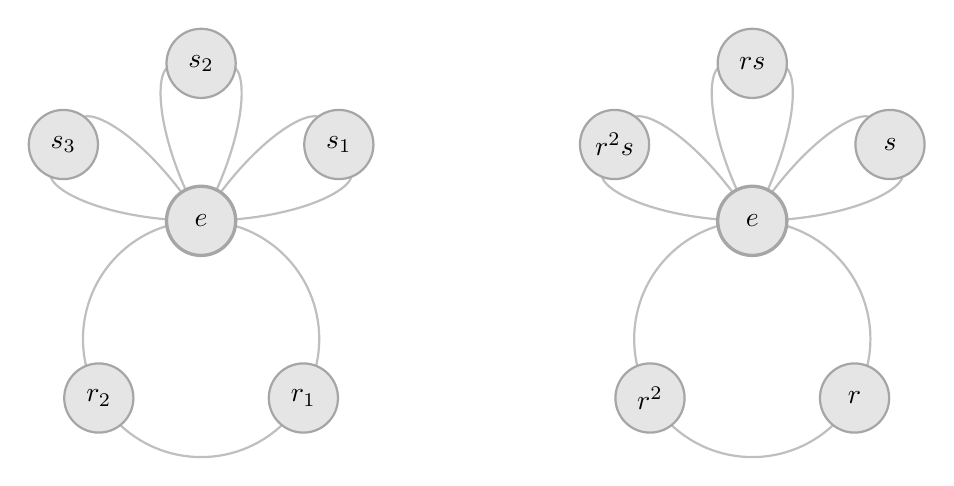
\begin{tikzpicture}[thick, font=\normalsize]
    \begin{scope}[shift={(0,0)}]

        % ===== 主环道（正圆）=====
        \draw[thick, gray!50] (0, -1.5) circle (1.5);

        % 主环道节点
        \node[circle, fill=gray!20, draw=gray!70, thick, inner sep=1.8pt, minimum size=25] at (1.299, -2.25) {$r_1$};
        \node[circle, fill=gray!20, draw=gray!70, thick, inner sep=1.8pt, minimum size=25] at (-1.299, -2.25) {$r_2$};

        % ===== 伴随环道（泪滴线）=====
        % --- 伴随环道 1（中心角 29.00°）---
        \draw[thick, gray!50] plot coordinates {(0, 0) (0.1036, 0.001) (0.2069, 0.0042) (0.3096, 0.0094) (0.4114, 0.0167) (0.5119, 0.0259) (0.6109, 0.0372) (0.7081, 0.0503) (0.8032, 0.0652) (0.8958, 0.0818) (0.9858, 0.1001) (1.0729, 0.12) (1.1568, 0.1412) (1.2372, 0.1638) (1.314, 0.1875) (1.3869, 0.2122) (1.4557, 0.2379) (1.5202, 0.2642) (1.5803, 0.2912) (1.6357, 0.3185) (1.6863, 0.3462) (1.732, 0.3738) (1.7727, 0.4014) (1.8083, 0.4288) (1.8386, 0.4557) (1.8636, 0.482) (1.8833, 0.5074) (1.8976, 0.532) (1.9065, 0.5553) (1.9101, 0.5774) (1.9082, 0.598) (1.9023, 0.6174) (1.896, 0.6366) (1.8894, 0.6558) (1.8827, 0.6748) (1.8758, 0.6939) (1.8687, 0.7128) (1.8613, 0.7317) (1.8538, 0.7505) (1.8462, 0.7692) (1.8383, 0.7879) (1.8302, 0.8065) (1.8219, 0.8249) (1.8135, 0.8433) (1.8049, 0.8617) (1.7961, 0.8799) (1.7871, 0.898) (1.7779, 0.9161) (1.7685, 0.934) (1.759, 0.9519) (1.7492, 0.9696) (1.7393, 0.9873) (1.7293, 1.0048) (1.719, 1.0223) (1.7086, 1.0396) (1.6979, 1.0569) (1.6872, 1.074) (1.6762, 1.091) (1.6651, 1.1079) (1.6538, 1.1247) (1.6423, 1.1414) (1.6307, 1.158) (1.6189, 1.1744) (1.6069, 1.1908) (1.5947, 1.207) (1.5824, 1.2231) (1.57, 1.239) (1.5574, 1.2548) (1.5446, 1.2705) (1.5316, 1.2861) (1.5184, 1.3014) (1.5019, 1.3139) (1.4813, 1.3225) (1.4567, 1.3274) (1.4283, 1.3282) (1.3963, 1.325) (1.3607, 1.3177) (1.3219, 1.3063) (1.2798, 1.2906) (1.2349, 1.2707) (1.1872, 1.2467) (1.1369, 1.2183) (1.0844, 1.1859) (1.0297, 1.1492) (0.9731, 1.1085) (0.9149, 1.0637) (0.8553, 1.015) (0.7945, 0.9625) (0.7328, 0.9062) (0.6703, 0.8463) (0.6073, 0.783) (0.5441, 0.7163) (0.4809, 0.6466) (0.4179, 0.5739) (0.3552, 0.4984) (0.2933, 0.4204) (0.2321, 0.34) (0.1721, 0.2576) (0.1132, 0.1733) (0.0558, 0.0873) (0, 0)};
        \node[circle, fill=gray!20, draw=gray!70, thick, inner sep=1.8pt, minimum size=25] at (1.7492, 0.9696) {$s_1$};

        % --- 伴随环道 2（中心角 90.00°）---
        \draw[thick, gray!50] plot coordinates {(0, 0) (0.0493, 0.0911) (0.0967, 0.183) (0.1419, 0.2754) (0.1849, 0.3679) (0.2255, 0.4603) (0.2637, 0.5523) (0.2993, 0.6437) (0.3324, 0.7341) (0.3627, 0.8232) (0.3904, 0.9108) (0.4152, 0.9966) (0.4373, 1.0802) (0.4566, 1.1615) (0.4731, 1.2402) (0.4868, 1.3159) (0.4977, 1.3885) (0.5059, 1.4577) (0.5115, 1.5233) (0.5144, 1.585) (0.5148, 1.6427) (0.5127, 1.6961) (0.5083, 1.7451) (0.5016, 1.7894) (0.4928, 1.829) (0.482, 1.8636) (0.4692, 1.8932) (0.4547, 1.9176) (0.4386, 1.9367) (0.421, 1.9505) (0.4021, 1.9589) (0.3823, 1.9631) (0.3624, 1.9669) (0.3425, 1.9705) (0.3225, 1.9738) (0.3025, 1.977) (0.2825, 1.9799) (0.2624, 1.9827) (0.2424, 1.9853) (0.2222, 1.9876) (0.2021, 1.9898) (0.182, 1.9917) (0.1618, 1.9934) (0.1416, 1.995) (0.1214, 1.9963) (0.1012, 1.9974) (0.081, 1.9984) (0.0607, 1.9991) (0.0405, 1.9996) (0.0202, 1.9999) (0, 2) (-0.0202, 1.9999) (-0.0405, 1.9996) (-0.0607, 1.9991) (-0.081, 1.9984) (-0.1012, 1.9974) (-0.1214, 1.9963) (-0.1416, 1.995) (-0.1618, 1.9934) (-0.182, 1.9917) (-0.2021, 1.9898) (-0.2222, 1.9876) (-0.2424, 1.9853) (-0.2624, 1.9827) (-0.2825, 1.9799) (-0.3025, 1.977) (-0.3225, 1.9738) (-0.3425, 1.9705) (-0.3624, 1.9669) (-0.3823, 1.9631) (-0.4021, 1.9589) (-0.421, 1.9505) (-0.4386, 1.9367) (-0.4547, 1.9176) (-0.4692, 1.8932) (-0.482, 1.8636) (-0.4928, 1.829) (-0.5016, 1.7894) (-0.5083, 1.7451) (-0.5127, 1.6961) (-0.5148, 1.6427) (-0.5144, 1.585) (-0.5115, 1.5233) (-0.5059, 1.4577) (-0.4977, 1.3885) (-0.4868, 1.3159) (-0.4731, 1.2402) (-0.4566, 1.1615) (-0.4373, 1.0802) (-0.4152, 0.9966) (-0.3904, 0.9108) (-0.3627, 0.8232) (-0.3324, 0.7341) (-0.2993, 0.6437) (-0.2637, 0.5523) (-0.2255, 0.4603) (-0.1849, 0.3679) (-0.1419, 0.2754) (-0.0967, 0.183) (-0.0493, 0.0911) (0, 0)};
        \node[circle, fill=gray!20, draw=gray!70, thick, inner sep=1.8pt, minimum size=25] at (0, 2) {$s_2$};

        % --- 伴随环道 3（中心角 151.00°）---
        \draw[thick, gray!50] plot coordinates {(0, 0) (-0.0558, 0.0873) (-0.1132, 0.1733) (-0.1721, 0.2576) (-0.2321, 0.34) (-0.2933, 0.4204) (-0.3552, 0.4984) (-0.4179, 0.5739) (-0.4809, 0.6466) (-0.5441, 0.7163) (-0.6073, 0.783) (-0.6703, 0.8463) (-0.7328, 0.9062) (-0.7945, 0.9625) (-0.8553, 1.015) (-0.9149, 1.0637) (-0.9731, 1.1085) (-1.0297, 1.1492) (-1.0844, 1.1859) (-1.1369, 1.2183) (-1.1872, 1.2467) (-1.2349, 1.2707) (-1.2798, 1.2906) (-1.3219, 1.3063) (-1.3607, 1.3177) (-1.3963, 1.325) (-1.4283, 1.3282) (-1.4567, 1.3274) (-1.4813, 1.3225) (-1.5019, 1.3139) (-1.5184, 1.3014) (-1.5316, 1.2861) (-1.5446, 1.2705) (-1.5574, 1.2548) (-1.57, 1.239) (-1.5824, 1.2231) (-1.5947, 1.207) (-1.6069, 1.1908) (-1.6189, 1.1744) (-1.6307, 1.158) (-1.6423, 1.1414) (-1.6538, 1.1247) (-1.6651, 1.1079) (-1.6762, 1.091) (-1.6872, 1.074) (-1.6979, 1.0569) (-1.7086, 1.0396) (-1.719, 1.0223) (-1.7293, 1.0048) (-1.7393, 0.9873) (-1.7492, 0.9696) (-1.759, 0.9519) (-1.7685, 0.934) (-1.7779, 0.9161) (-1.7871, 0.898) (-1.7961, 0.8799) (-1.8049, 0.8617) (-1.8135, 0.8433) (-1.8219, 0.8249) (-1.8302, 0.8065) (-1.8383, 0.7879) (-1.8462, 0.7692) (-1.8538, 0.7505) (-1.8613, 0.7317) (-1.8687, 0.7128) (-1.8758, 0.6939) (-1.8827, 0.6748) (-1.8894, 0.6558) (-1.896, 0.6366) (-1.9023, 0.6174) (-1.9082, 0.598) (-1.9101, 0.5774) (-1.9065, 0.5553) (-1.8976, 0.532) (-1.8833, 0.5074) (-1.8636, 0.482) (-1.8386, 0.4557) (-1.8083, 0.4288) (-1.7727, 0.4014) (-1.732, 0.3738) (-1.6863, 0.3462) (-1.6357, 0.3185) (-1.5803, 0.2912) (-1.5202, 0.2642) (-1.4557, 0.2379) (-1.3869, 0.2122) (-1.314, 0.1875) (-1.2372, 0.1638) (-1.1568, 0.1412) (-1.0729, 0.12) (-0.9858, 0.1001) (-0.8958, 0.0818) (-0.8032, 0.0652) (-0.7081, 0.0503) (-0.6109, 0.0372) (-0.5119, 0.0259) (-0.4114, 0.0167) (-0.3096, 0.0094) (-0.2069, 0.0042) (-0.1036, 0.001) (0, 0)};
        \node[circle, fill=gray!20, draw=gray!70, thick, inner sep=1.8pt, minimum size=25] at (-1.7492, 0.9696) {$s_3$};

        % ===== 幺元 =====
        \node[circle, fill=gray!20, draw=gray!70, very thick, inner sep=2pt, minimum size=25] at (0, 0) {$e$};

    \end{scope}
    \begin{scope}[shift={(7,0)}]

        % ===== 主环道（正圆）=====
        \draw[thick, gray!50] (0, -1.5) circle (1.5);

        % 主环道节点
        \node[circle, fill=gray!20, draw=gray!70, thick, inner sep=1.8pt, minimum size=25] at (1.299, -2.25) {$r$};
        \node[circle, fill=gray!20, draw=gray!70, thick, inner sep=1.8pt, minimum size=25] at (-1.299, -2.25) {$r^2$};

        % ===== 伴随环道（泪滴线）=====
        % --- 伴随环道 1（中心角 29.00°）---
        \draw[thick, gray!50] plot coordinates {(0, 0) (0.1036, 0.001) (0.2069, 0.0042) (0.3096, 0.0094) (0.4114, 0.0167) (0.5119, 0.0259) (0.6109, 0.0372) (0.7081, 0.0503) (0.8032, 0.0652) (0.8958, 0.0818) (0.9858, 0.1001) (1.0729, 0.12) (1.1568, 0.1412) (1.2372, 0.1638) (1.314, 0.1875) (1.3869, 0.2122) (1.4557, 0.2379) (1.5202, 0.2642) (1.5803, 0.2912) (1.6357, 0.3185) (1.6863, 0.3462) (1.732, 0.3738) (1.7727, 0.4014) (1.8083, 0.4288) (1.8386, 0.4557) (1.8636, 0.482) (1.8833, 0.5074) (1.8976, 0.532) (1.9065, 0.5553) (1.9101, 0.5774) (1.9082, 0.598) (1.9023, 0.6174) (1.896, 0.6366) (1.8894, 0.6558) (1.8827, 0.6748) (1.8758, 0.6939) (1.8687, 0.7128) (1.8613, 0.7317) (1.8538, 0.7505) (1.8462, 0.7692) (1.8383, 0.7879) (1.8302, 0.8065) (1.8219, 0.8249) (1.8135, 0.8433) (1.8049, 0.8617) (1.7961, 0.8799) (1.7871, 0.898) (1.7779, 0.9161) (1.7685, 0.934) (1.759, 0.9519) (1.7492, 0.9696) (1.7393, 0.9873) (1.7293, 1.0048) (1.719, 1.0223) (1.7086, 1.0396) (1.6979, 1.0569) (1.6872, 1.074) (1.6762, 1.091) (1.6651, 1.1079) (1.6538, 1.1247) (1.6423, 1.1414) (1.6307, 1.158) (1.6189, 1.1744) (1.6069, 1.1908) (1.5947, 1.207) (1.5824, 1.2231) (1.57, 1.239) (1.5574, 1.2548) (1.5446, 1.2705) (1.5316, 1.2861) (1.5184, 1.3014) (1.5019, 1.3139) (1.4813, 1.3225) (1.4567, 1.3274) (1.4283, 1.3282) (1.3963, 1.325) (1.3607, 1.3177) (1.3219, 1.3063) (1.2798, 1.2906) (1.2349, 1.2707) (1.1872, 1.2467) (1.1369, 1.2183) (1.0844, 1.1859) (1.0297, 1.1492) (0.9731, 1.1085) (0.9149, 1.0637) (0.8553, 1.015) (0.7945, 0.9625) (0.7328, 0.9062) (0.6703, 0.8463) (0.6073, 0.783) (0.5441, 0.7163) (0.4809, 0.6466) (0.4179, 0.5739) (0.3552, 0.4984) (0.2933, 0.4204) (0.2321, 0.34) (0.1721, 0.2576) (0.1132, 0.1733) (0.0558, 0.0873) (0, 0)};
        \node[circle, fill=gray!20, draw=gray!70, thick, inner sep=1.8pt, minimum size=25] at (1.7492, 0.9696) {$s$};

        % --- 伴随环道 2（中心角 90.00°）---
        \draw[thick, gray!50] plot coordinates {(0, 0) (0.0493, 0.0911) (0.0967, 0.183) (0.1419, 0.2754) (0.1849, 0.3679) (0.2255, 0.4603) (0.2637, 0.5523) (0.2993, 0.6437) (0.3324, 0.7341) (0.3627, 0.8232) (0.3904, 0.9108) (0.4152, 0.9966) (0.4373, 1.0802) (0.4566, 1.1615) (0.4731, 1.2402) (0.4868, 1.3159) (0.4977, 1.3885) (0.5059, 1.4577) (0.5115, 1.5233) (0.5144, 1.585) (0.5148, 1.6427) (0.5127, 1.6961) (0.5083, 1.7451) (0.5016, 1.7894) (0.4928, 1.829) (0.482, 1.8636) (0.4692, 1.8932) (0.4547, 1.9176) (0.4386, 1.9367) (0.421, 1.9505) (0.4021, 1.9589) (0.3823, 1.9631) (0.3624, 1.9669) (0.3425, 1.9705) (0.3225, 1.9738) (0.3025, 1.977) (0.2825, 1.9799) (0.2624, 1.9827) (0.2424, 1.9853) (0.2222, 1.9876) (0.2021, 1.9898) (0.182, 1.9917) (0.1618, 1.9934) (0.1416, 1.995) (0.1214, 1.9963) (0.1012, 1.9974) (0.081, 1.9984) (0.0607, 1.9991) (0.0405, 1.9996) (0.0202, 1.9999) (0, 2) (-0.0202, 1.9999) (-0.0405, 1.9996) (-0.0607, 1.9991) (-0.081, 1.9984) (-0.1012, 1.9974) (-0.1214, 1.9963) (-0.1416, 1.995) (-0.1618, 1.9934) (-0.182, 1.9917) (-0.2021, 1.9898) (-0.2222, 1.9876) (-0.2424, 1.9853) (-0.2624, 1.9827) (-0.2825, 1.9799) (-0.3025, 1.977) (-0.3225, 1.9738) (-0.3425, 1.9705) (-0.3624, 1.9669) (-0.3823, 1.9631) (-0.4021, 1.9589) (-0.421, 1.9505) (-0.4386, 1.9367) (-0.4547, 1.9176) (-0.4692, 1.8932) (-0.482, 1.8636) (-0.4928, 1.829) (-0.5016, 1.7894) (-0.5083, 1.7451) (-0.5127, 1.6961) (-0.5148, 1.6427) (-0.5144, 1.585) (-0.5115, 1.5233) (-0.5059, 1.4577) (-0.4977, 1.3885) (-0.4868, 1.3159) (-0.4731, 1.2402) (-0.4566, 1.1615) (-0.4373, 1.0802) (-0.4152, 0.9966) (-0.3904, 0.9108) (-0.3627, 0.8232) (-0.3324, 0.7341) (-0.2993, 0.6437) (-0.2637, 0.5523) (-0.2255, 0.4603) (-0.1849, 0.3679) (-0.1419, 0.2754) (-0.0967, 0.183) (-0.0493, 0.0911) (0, 0)};
        \node[circle, fill=gray!20, draw=gray!70, thick, inner sep=1.8pt, minimum size=25] at (0, 2) {$rs$};

        % --- 伴随环道 3（中心角 151.00°）---
        \draw[thick, gray!50] plot coordinates {(0, 0) (-0.0558, 0.0873) (-0.1132, 0.1733) (-0.1721, 0.2576) (-0.2321, 0.34) (-0.2933, 0.4204) (-0.3552, 0.4984) (-0.4179, 0.5739) (-0.4809, 0.6466) (-0.5441, 0.7163) (-0.6073, 0.783) (-0.6703, 0.8463) (-0.7328, 0.9062) (-0.7945, 0.9625) (-0.8553, 1.015) (-0.9149, 1.0637) (-0.9731, 1.1085) (-1.0297, 1.1492) (-1.0844, 1.1859) (-1.1369, 1.2183) (-1.1872, 1.2467) (-1.2349, 1.2707) (-1.2798, 1.2906) (-1.3219, 1.3063) (-1.3607, 1.3177) (-1.3963, 1.325) (-1.4283, 1.3282) (-1.4567, 1.3274) (-1.4813, 1.3225) (-1.5019, 1.3139) (-1.5184, 1.3014) (-1.5316, 1.2861) (-1.5446, 1.2705) (-1.5574, 1.2548) (-1.57, 1.239) (-1.5824, 1.2231) (-1.5947, 1.207) (-1.6069, 1.1908) (-1.6189, 1.1744) (-1.6307, 1.158) (-1.6423, 1.1414) (-1.6538, 1.1247) (-1.6651, 1.1079) (-1.6762, 1.091) (-1.6872, 1.074) (-1.6979, 1.0569) (-1.7086, 1.0396) (-1.719, 1.0223) (-1.7293, 1.0048) (-1.7393, 0.9873) (-1.7492, 0.9696) (-1.759, 0.9519) (-1.7685, 0.934) (-1.7779, 0.9161) (-1.7871, 0.898) (-1.7961, 0.8799) (-1.8049, 0.8617) (-1.8135, 0.8433) (-1.8219, 0.8249) (-1.8302, 0.8065) (-1.8383, 0.7879) (-1.8462, 0.7692) (-1.8538, 0.7505) (-1.8613, 0.7317) (-1.8687, 0.7128) (-1.8758, 0.6939) (-1.8827, 0.6748) (-1.8894, 0.6558) (-1.896, 0.6366) (-1.9023, 0.6174) (-1.9082, 0.598) (-1.9101, 0.5774) (-1.9065, 0.5553) (-1.8976, 0.532) (-1.8833, 0.5074) (-1.8636, 0.482) (-1.8386, 0.4557) (-1.8083, 0.4288) (-1.7727, 0.4014) (-1.732, 0.3738) (-1.6863, 0.3462) (-1.6357, 0.3185) (-1.5803, 0.2912) (-1.5202, 0.2642) (-1.4557, 0.2379) (-1.3869, 0.2122) (-1.314, 0.1875) (-1.2372, 0.1638) (-1.1568, 0.1412) (-1.0729, 0.12) (-0.9858, 0.1001) (-0.8958, 0.0818) (-0.8032, 0.0652) (-0.7081, 0.0503) (-0.6109, 0.0372) (-0.5119, 0.0259) (-0.4114, 0.0167) (-0.3096, 0.0094) (-0.2069, 0.0042) (-0.1036, 0.001) (0, 0)};
        \node[circle, fill=gray!20, draw=gray!70, thick, inner sep=1.8pt, minimum size=25] at (-1.7492, 0.9696) {$r^2s$};

        % ===== 幺元 =====
        \node[circle, fill=gray!20, draw=gray!70, very thick, inner sep=2pt, minimum size=25] at (0, 0) {$e$};

    \end{scope}
    \end{tikzpicture}
    \caption{\texttt{映轮群 $\mathsf{D}_3$ 的环道图}}
    \label{fig:D3OrbitDiagram}
\end{figure}

群的每个元素都有自己所属的环道。我们把$e$看作“原点”。从$e$出发，每次根据不同元素的环道，要么沿着环道走一个圈，再回到$e$；要么得到序列：
$$ a^{-n}, \cdots, a^{-2}, a^{-1}, e, a, a^2, \cdots, a^n,  \cdots $$
我们可以把它看作“直线”。这样我们可以生成整个群。这样按照环道循环画出来的生成路径图也叫\textbf{环道图}。比如上图是三元对称群$\mathsf{D}_3$的环道图。为了方便，只记录$r=r_1$，$r_2=r_1^2=r^2$。它们和$e$构成三元环道。三个翻转变换$s_1,s_2,s_3$（记为$s_1=s,s_2=rs,s_3=r^2s$）则分别对应二元环道。

\section{交换群}

一个群的变换如果能够任意交换顺序而效果不变，就说是它是交换群。循环群就是一种交换群（是一种基本而常见的交换群）。考虑生成循环群的变换$a$，其他的变换都是它重复的结果。所以无非是先重复几次、后重复几次的区别，交换顺序并不改变最终的效果。“朝三暮四”的成语用在这里正合适。

如何看一个群是不是交换群呢？首先我们可以观察它的连线图（最好是完全连线图）。从任一节点（状态）出发，先通过变换$a$再通过变换$b$到达的节点，是否和先通过变换$b$再通过变换$a$到达的节点一样？如果能找到不一样的情况，就说明它不是交换群。如果总是一样，那么它就是交换群了。

% 插图，解释以上的检验方法
\vspace{12pt}
\begin{figure}[htbp]
    \centering
    \begin{tikzpicture}[>=Stealth, thick, font=\normalsize]
    \begin{scope}[shift={(0,0)}]
        \def\A{1.0}
        \def\B{1.5}
        % 状态节点
        \node[circle, fill=gray!5, draw=darkgray, thick, inner sep=1.8pt, minimum size=25] (A1) at (0,0) {};
        \node[circle, fill=gray!5, draw=darkgray, thick, inner sep=1.8pt, minimum size=25] (A2) at (\B, -\A) {};
        \node[circle, fill=gray!5, draw=darkgray, thick, inner sep=1.8pt, minimum size=25] (A3) at (\B, \A) {};
        \node[circle, fill=gray!5, draw=darkgray, thick, inner sep=1.8pt, minimum size=25] (A4) at (2*\B, 0) {};
        \draw[->] (A1) -- node[below left=-0.1cm] {$a$} (A2);
        \draw[->] (A1) -- node[above left=-0.1cm] {$b$} (A3);
        \draw[->] (A2) -- node[below] {$b$} (A4);
        \draw[->] (A3) -- node[above] {$a$} (A4);
        \draw (\B, -\A-1) node {\texttt{先$a$后$b$和}\phantom{呵呵呵}};
        \draw (\B, -\A-1.5) node {\texttt{先$b$后$a$效果相同}};

    \end{scope}
    \begin{scope}[shift={(7,0)}]
        \def\A{1.0}
        \def\B{1.8}
        % 状态节点
        \node[circle, fill=gray!5, draw=darkgray, thick, inner sep=1.8pt, minimum size=25] (A1) at (0,0) {};
        \node[circle, fill=gray!5, draw=darkgray, thick, inner sep=1.8pt, minimum size=25] (A2) at (\B, -\A) {};
        \node[circle, fill=gray!5, draw=darkgray, thick, inner sep=1.8pt, minimum size=25] (A3) at (\B, \A) {};
        \node[circle, fill=gray!5, draw=darkgray, thick, inner sep=1.8pt, minimum size=25] (A4) at (2*\B, -\A) {};
        \node[circle, fill=gray!5, draw=darkgray, thick, inner sep=1.8pt, minimum size=25] (A5) at (2*\B, \A) {};
        \draw[->] (A1) -- node[below left=-0.1cm] {$a$} (A2);
        \draw[->] (A1) -- node[above left=-0.1cm] {$b$} (A3);
        \draw[->] (A2) -- node[below] {$b$} (A4);
        \draw[->] (A3) -- node[above] {$a$} (A5);
        \draw (\B, -\A-1) node {\texttt{先$a$后$b$和}\phantom{呵呵呵}};
        \draw (\B, -\A-1.5) node {\texttt{先$b$后$a$效果不同}};

    \end{scope}
    \end{tikzpicture}
    \label{fig:explain_commutativity}
\end{figure}
\vspace{12pt}

另一种方法是查看它的乘法表。交换群的变换可以交换顺序：$ab = ba$，在乘法表里就体现在第$i$行第$j$列的内容与第$j$行第$ji$列的内容相同（前提是在行头和列头按同样的顺序排列群里的变换——第$i$行的行头和第$i$列的列头应该是同样的变换）。直观来看，如果把乘法表按着主对角线（从左上到右下的对角线）折叠，对角线两侧的变换刚好重叠。或者说，沿主对角线翻转，乘法表内容不变。这也是一种对称性的体现——乘法表的对称性对应着乘法先后顺序可交换的对称性。

% 插图，解释以上的检验方法
\vspace{12pt}
\begin{figure}[htbp]
    \centering
    \begin{tikzpicture}[scale=0.8,>=Stealth, thick, font=\normalsize]
    \begin{scope}[shift={(0,0)}]
        \def\x{0.7}
        \def\y{0.7}
        \def\n{8}
        \def\ii{3}
        \def\jj{5}
        \def\pad{0.15}

        \draw[thick, darkgray] (0,0) -- (\n*\x, 0) -- (\n*\x, -\n*\y) --(0, -\n*\y) -- cycle;
        \fill[thick, color=gray!10] (0,0) -- (\n*\x, -\n*\y) --(0, -\n*\y) -- cycle;
        \filldraw[thick, color=gray!5, draw=darkgray] (0,\pad) rectangle (\n*\x,\pad+\y);
        \filldraw[thick, color=gray!5, draw=darkgray] (-\pad,0) rectangle (-\pad-\x,-\n*\y);
        \draw[thick,darkgray] (\ii*\x,\pad) rectangle (\ii*\x+\x,\pad+\y);
        \draw[thick,darkgray] (\jj*\x,\pad) rectangle (\jj*\x+\x,\pad+\y);
        \draw[thick,darkgray] (-\pad,-\jj*\y) rectangle (-\pad-\x,-\jj*\y-\y);
        \draw[thick,darkgray] (-\pad,-\ii*\y) rectangle (-\pad-\x,-\ii*\y-\y);
        \node at (\ii*\x+0.5*\x,\pad+0.5*\y) {$a$};
        \node at (\jj*\x+0.5*\x,\pad+0.5*\y) {$b$};
        \node at (-\pad-0.5*\x,-\ii*\y-0.5*\y) {$a$};
        \node at (-\pad-0.5*\x,-\jj*\y-0.5*\y) {$b$};
        \draw[thick,darkgray] (\ii*\x,-\jj*\y) rectangle (\ii*\x+\x,-\jj*\y-\y);
        \draw[thick,darkgray] (\jj*\x,-\ii*\y) rectangle (\jj*\x+\x,-\ii*\y-\y);
        \node at (\ii*\x+0.5*\x,-\jj*\y-0.5*\y) {$ab$};
        \node at (\jj*\x+0.5*\x,-\ii*\y-0.5*\y) {$ba$};
        \draw[->, dashed] (\ii*\x+0.5*\x,-\pad) -- (\ii*\x+0.5*\x,-\jj*\y+\pad);
        \draw[->, dashed] (\jj*\x+0.5*\x,-\pad) -- (\jj*\x+0.5*\x,-\ii*\y+\pad);
        \draw[->, dashed] (\pad,-\ii*\y-0.5*\y) -- (\jj*\x-\pad,-\ii*\y-0.5*\y);
        \draw[->, dashed] (\pad,-\jj*\y-0.5*\y) -- (\ii*\x-\pad,-\jj*\y-0.5*\y);
        \draw[<->] (\ii*\x+0.5*\x,-\ii*\y-0.5*\y) ++ (-20:\jj*\y-\ii*\x) arc (-20:-70:\jj*\y-\ii*\x);
        \node[rotate=45] at (\jj*\x+0.5*\x,-\jj*\y-0.5*\y) {\texttt{是否相等}};

    \end{scope}
    \end{tikzpicture}
    \label{fig:explain_commutativity_table}
    \caption{\texttt{检查群的乘法表：主对角线两侧对应的格子，元素是否相等}}
\end{figure}

除了循环群，还有哪些交换群的例子呢？交换群的一个重要场景是晶体的微观结构。什么是晶体呢？晶体是一种固体，构成它的最小粒子在空间中按照一个固定的模式不断重复排列。你可以想象在立体空间里搭起一个无限延伸的脚手架，构成一个个一模一样排列的格子，每个格点上放一个完全相同的小球。无论你站在这个手脚架的哪个位置，向任何方向看，看到的排列方式都完全一样。这种“无限重复、处处相同”的规律就是典型的晶体的特征。

以食盐（氯化钠）为例：钠离子和氯离子交替排列，形成一个个小立方体，每个钠离子上下左右前后都是氯离子，每个氯离子上下左右前后都是钠离子。我们可以建立一个理想的模型。在模型里，这个立方体网格向上下、前后、左右无限重复。因此，我们如果将整个网格整体往上平移两个小立方体边长的距离（以下称为“一格”），会得到完全一样的网格。同理，整体往下、往左、往右、往前、往后平移一格，也会得到完全一样的网格。我们把这样的平移变换视为群的元素，生成的群称为\textbf{立体平移群}或\textbf{空间平移群}。

% 插图 氯化钠的晶体结构\vspace{12pt}
\begin{figure}[htbp]
    \centering
    \begin{tikzpicture}[>=Stealth]
    \begin{scope}[shift={(0,0)}]
    % ============================================================
    % Crystal parameters
    % ============================================================

    \def\N{4}
    \pgfmathtruncatemacro{\Nm}{\N-1}

    % ============================================================
    % Perspective parameters
    % ============================================================

    % Distance from the crystal to the camera
    %
    % Larger = weaker perspective
    % Smaller = stronger perspective
    %
    \def\CameraDistance{10}

    % Direction of the receding y-axis in the drawing.
    %
    % VPX, VPY = vanishing point
    %
    \def\VPX{3.8}
    \def\VPY{0.5}

    % Overall scale
    \def\ScaleFactor{1.0}

    % ============================================================
    % Ion appearance
    % ============================================================

    \def\ClRadius{0.13}
    \def\NaRadius{0.095}

    \colorlet{ClColor}{gray!65}
    \colorlet{NaColor}{orange!85}

    % ============================================================
    % Bonds
    % ============================================================

    \colorlet{BondColor}{gray!55}
    \def\BondWidth{0.7pt}


    % ============================================================
    % Projection
    % ============================================================
    %
    % World coordinates:
    %
    %       x : horizontal crystal direction
    %       y : depth / receding direction
    %       z : vertical crystal direction
    %
    % We use a one-point perspective projection.
    %
    % The perspective factor is
    %
    %       s = D / (D + y)
    %
    % where D is the camera distance.
    %
    % For y > 0, points are farther away and therefore smaller.
    %
    % The point y = infinity approaches the vanishing point.
    %
    % ============================================================


    % ------------------------------------------------------------
    % Projection of a point
    % ------------------------------------------------------------
    %
    % We use:
    %
    %       X = VPX + s * (x - VPX)
    %       Y = VPY + s * (z - VPY)
    %
    % Thus the point (x,z) is pulled toward the vanishing point
    % as its depth y increases.
    %
    % ------------------------------------------------------------


    % ============================================================
    % Draw bonds
    % ============================================================

    % ------------------------------------------------------------
    % x-direction bonds
    % ------------------------------------------

    \foreach \i in {0,...,\Nm}
    \foreach \j in {0,...,\N}
        \foreach \k in {0,...,\N}{%

        % Centre crystal around y = 0
        \pgfmathsetmacro{\xA}{\i-\N/2}
        \pgfmathsetmacro{\yA}{\j-\N/2}
        \pgfmathsetmacro{\zA}{\k-\N/2}

        \pgfmathsetmacro{\sA}{%
            \CameraDistance/
            (\CameraDistance+\yA)
        }

        \pgfmathsetmacro{\XA}{%
            \ScaleFactor*
            (\VPX+\sA*(\xA-\VPX))
        }

        \pgfmathsetmacro{\YA}{%
            \ScaleFactor*
            (\VPY+\sA*(\zA-\VPY))
        }


        % Second point
        \pgfmathsetmacro{\xB}{\i+1-\N/2}
        \pgfmathsetmacro{\yB}{\j-\N/2}
        \pgfmathsetmacro{\zB}{\k-\N/2}

        \pgfmathsetmacro{\sB}{%
            \CameraDistance/
            (\CameraDistance+\yB)
        }

        \pgfmathsetmacro{\XB}{%
            \ScaleFactor*
            (\VPX+\sB*(\xB-\VPX))
        }

        \pgfmathsetmacro{\YB}{%
            \ScaleFactor*
            (\VPY+\sB*(\zB-\VPY))
        }

        \draw[
            BondColor,
            line width=\BondWidth
        ] (\XA,\YA) -- (\XB,\YB);
        }


    % ------------------------------------------------------------
    % y-direction bonds
    % ------------------------------------------------------------

    \foreach \i in {0,...,\N}
    \foreach \j in {0,...,\Nm}
        \foreach \k in {0,...,\N}{%

        % First point
        \pgfmathsetmacro{\xA}{\i-\N/2}
        \pgfmathsetmacro{\yA}{\j-\N/2}
        \pgfmathsetmacro{\zA}{\k-\N/2}

        \pgfmathsetmacro{\sA}{%
            \CameraDistance/
            (\CameraDistance+\yA)
        }

        \pgfmathsetmacro{\XA}{%
            \ScaleFactor*
            (\VPX+\sA*(\xA-\VPX))
        }

        \pgfmathsetmacro{\YA}{%
            \ScaleFactor*
            (\VPY+\sA*(\zA-\VPY))
        }


        % Second point
        \pgfmathsetmacro{\xB}{\i-\N/2}
        \pgfmathsetmacro{\yB}{\j+1-\N/2}
        \pgfmathsetmacro{\zB}{\k-\N/2}

        \pgfmathsetmacro{\sB}{%
            \CameraDistance/
            (\CameraDistance+\yB)
        }

        \pgfmathsetmacro{\XB}{%
            \ScaleFactor*
            (\VPX+\sB*(\xB-\VPX))
        }

        \pgfmathsetmacro{\YB}{%
            \ScaleFactor*
            (\VPY+\sB*(\zB-\VPY))
        }

        \draw[
            BondColor,
            line width=\BondWidth
        ] (\XA,\YA) -- (\XB,\YB);
        }


    % ------------------------------------------------------------
    % z-direction bonds
    % ------------------------------------------------------------

    \foreach \i in {0,...,\N}
    \foreach \j in {0,...,\N}
        \foreach \k in {0,...,\Nm}{%

        % First point
        \pgfmathsetmacro{\xA}{\i-\N/2}
        \pgfmathsetmacro{\yA}{\j-\N/2}
        \pgfmathsetmacro{\zA}{\k-\N/2}

        \pgfmathsetmacro{\sA}{%
            \CameraDistance/
            (\CameraDistance+\yA)
        }

        \pgfmathsetmacro{\XA}{%
            \ScaleFactor*
            (\VPX+\sA*(\xA-\VPX))
        }

        \pgfmathsetmacro{\YA}{%
            \ScaleFactor*
            (\VPY+\sA*(\zA-\VPY))
        }


        % Second point
        \pgfmathsetmacro{\xB}{\i-\N/2}
        \pgfmathsetmacro{\yB}{\j-\N/2}
        \pgfmathsetmacro{\zB}{\k+1-\N/2}

        \pgfmathsetmacro{\sB}{%
            \CameraDistance/
            (\CameraDistance+\yB)
        }

        \pgfmathsetmacro{\XB}{%
            \ScaleFactor*
            (\VPX+\sB*(\xB-\VPX))
        }

        \pgfmathsetmacro{\YB}{%
            \ScaleFactor*
            (\VPY+\sB*(\zB-\VPY))
        }

        \draw[
            BondColor,
            line width=\BondWidth
        ] (\XA,\YA) -- (\XB,\YB);
        }


    % ============================================================
    % Draw ions
    % ============================================================
    %
    % Back-to-front ordering in y.
    %
    % The smaller-y points are closer to the viewer if the camera
    % is at y = -CameraDistance.
    %
    % Therefore draw large y first and small y last.
    %
    % ============================================================

    \foreach \j in {\N,...,0}{%

    \foreach \k in {0,...,\N}{%

        \foreach \i in {0,...,\N}{%

        \pgfmathsetmacro{\x}{\i-\N/2}
        \pgfmathsetmacro{\y}{\j-\N/2}
        \pgfmathsetmacro{\z}{\k-\N/2}

        % Perspective scale
        \pgfmathsetmacro{\s}{%
            \CameraDistance/
            (\CameraDistance+\y)
        }

        % Projected coordinates
        \pgfmathsetmacro{\X}{%
            \ScaleFactor*
            (\VPX+\s*(\x-\VPX))
        }

        \pgfmathsetmacro{\Y}{%
            \ScaleFactor*
            (\VPY+\s*(\z-\VPY))
        }

        % NaCl alternating lattice
        \pgfmathtruncatemacro{\p}{mod(\i+\j+\k,2)}

        \ifnum\p=0

            \pgfmathsetmacro{\r}{\ClRadius*\s}

            \shade[
            ball color=ClColor
            ] (\X,\Y) circle (\r);

        \else

            \pgfmathsetmacro{\r}{\NaRadius*\s}

            \shade[
            ball color=NaColor
            ] (\X,\Y) circle (\r);

        \fi
        }
    }
    }


    % ============================================================
    % Legend
    % ============================================================

    \shade[
    ball color=ClColor
    ] (-0.35,3.25) circle (\ClRadius);

    \node[
    anchor=west
    ] at (-0.18,3.25) {$\mathrm{Cl^-}$};


    \shade[
    ball color=NaColor
    ] (1.15,3.25) circle (\NaRadius);

    \node[
    anchor=west
    ] at (1.28,3.25) {$\mathrm{Na^+}$};

    \draw[->,thick] (-3.9,-2.7) -- (-3.9,-0.1);
    \draw[->,thick] (-3.5, -3) -- (-.9,-3);
    \draw[->,thick] (-3.9,-2.7) -- (-2.23,-1.98);
    \node at (-4.2, -1.2) {\texttt{向}};
    \node at (-4.2, -1.6) {\texttt{上}};
    \node at (-2.2, -3.3) {\texttt{向右}};
    \node[rotate=20] at (-3.3, -2.1) {\texttt{向前}};
    \end{scope}
    \begin{scope}[scale=1.25,shift={(3,-2.1)}]

    % ============================================================
    % Parameters
    % ============================================================

    % Number of lattice intervals
    \def\N{4}

    % Overall scale
    \def\Scale{1.0}

    % ------------------------------------------------------------
    % One-point perspective
    % ------------------------------------------------------------

    % Camera distance.
    % Larger = weaker perspective.
    % Smaller = stronger perspective.
    \def\CameraDistance{10}

    % Position of the vanishing point.
    %
    % All lines parallel to the y-axis converge here.
    \def\VPX{5.8}
    \def\VPY{2.5}

    % ------------------------------------------------------------
    % Coordinate-system appearance
    % ------------------------------------------------------------

    \def\AxisWidth{1.0pt}
    \def\GridWidth{0.45pt}

    % Length of the coordinate axes
    \def\AxisExtension{1.0}

    % ------------------------------------------------------------
    % Lattice points
    % ------------------------------------------------------------

    \def\PointRadius{1.3pt}


    % ============================================================
    % Projection function
    % ============================================================
    %
    % Crystal coordinates:
    %
    %       x = horizontal direction
    %       y = depth direction
    %       z = vertical direction
    %
    % The camera is on the negative-y side.
    %
    % For a point (x,y,z):
    %
    %       s = D / (D+y)
    %
    % and
    %
    %       X = VPX + s (x - VPX)
    %       Y = VPY + s (z - VPY)
    %
    % Therefore:
    %
    %   y = constant  --> parallel x-z planes
    %
    %   increasing y  --> the whole plane moves toward VP
    %
    %   y -> infinity --> VP
    %
    % ============================================================


    % ============================================================
    % Draw one projected point
    % ============================================================

    % We use a macro because it makes the lattice construction
    % below much easier to read.

    \newcommand{\ProjectPoint}[4]{%
    % #1 = x
    % #2 = y
    % #3 = z
    % #4 = macro prefix

    \pgfmathsetmacro{\s}{%
        \CameraDistance/
        (\CameraDistance+#2)
    }

    \pgfmathsetmacro{\PX}{%
        \Scale*
        (\VPX+\s*(#1-\VPX))
    }

    \pgfmathsetmacro{\PY}{%
        \Scale*
        (\VPY+\s*(#3-\VPY))
    }

    \coordinate (#4) at (\PX,\PY);
    }


    % ============================================================
    % Draw the lattice
    % ============================================================

    % We draw the lattice planes from back to front.
    %
    % y = N is the back plane
    % y = 0 is the front plane
    %
    % This is useful when later adding shaded planes or objects.

    \foreach \j in {\N,...,0}{%

    % ----------------------------------------------------------
    % Horizontal x-lines
    % ----------------------------------------------------------

    \foreach \k in {0,...,\N}{%

        \ProjectPoint{0}{\j}{\k}{A}
        \ProjectPoint{\N}{\j}{\k}{B}

        \draw[
        line width=\GridWidth,
        gray!55
        ] (A) -- (B);
    }


    % ----------------------------------------------------------
    % Vertical z-lines
    % ----------------------------------------------------------

    \foreach \i in {0,...,\N}{%

        \ProjectPoint{\i}{\j}{0}{A}
        \ProjectPoint{\i}{\j}{\N}{B}

        \draw[
        line width=\GridWidth,
        gray!55
        ] (A) -- (B);
    }
    }


    % ============================================================
    % Draw the receding y-lines
    % ============================================================

    % Every y-line must converge to the SAME vanishing point.

    \coordinate (VP) at
    (\Scale*\VPX,\Scale*\VPY);

    \foreach \i in {0,...,\N}{%
    \foreach \k in {0,...,\N}{%

        \ProjectPoint{\i}{0}{\k}{A}
        \ProjectPoint{\i}{\N}{\k}{B}

        \draw[
        line width=\GridWidth,
        gray!55
        ] (A) -- (B);
    }
    }


    % ============================================================
    % Lattice points
    % ============================================================

    % Draw them after the grid so they remain visible.

    % \foreach \j in {0,...,\N}{%
    %   \foreach \i in {0,...,\N}{%
    %     \foreach \k in {0,...,\N}{%

    %       \ProjectPoint{\i}{\j}{\k}{P}

    %       \fill
    %         (P)
    %         circle (\PointRadius);
    %     }
    %   }
    % }


    % ============================================================
    % Coordinate axes
    % ============================================================

    % We place the origin at (0,0,0).

    \ProjectPoint{0}{0}{0}{O}

    % ------------------------------------------------------------
    % x-axis
    % ------------------------------------------------------------

    \ProjectPoint{\N+\AxisExtension}{0}{0}{Xaxis}

    \draw[
    ->,
    line width=\AxisWidth
    ]
    (O) -- (Xaxis)
    node[
        below right,
        inner sep=2pt
    ] {$y$};


    % ------------------------------------------------------------
    % z-axis
    % ------------------------------------------------------------

    \ProjectPoint{0}{0}{\N+\AxisExtension}{Zaxis}

    \draw[
    ->,
    line width=\AxisWidth
    ]
    (O) -- (Zaxis)
    node[
        left,
        inner sep=2pt
    ] {$z$};


    % ------------------------------------------------------------
    % y-axis
    % ------------------------------------------------------------

    % The y-axis itself is drawn as a line toward the vanishing
    % point, but we stop before reaching it.

    \ProjectPoint{0}{\N+\AxisExtension}{0}{Yaxis}

    \draw[
    ->,
    line width=\AxisWidth
    ]
    (O) -- (Yaxis)
    node[
        below,
        inner sep=2pt
    ] {$x$};


    % ============================================================
    % Origin
    % ============================================================

    \node[
    below left,
    inner sep=2pt
    ]
    at (O) {$O$};


    % ============================================================
    % Vanishing point
    % ============================================================

    % Uncomment this if you want the vanishing point visible.
    %
    % \fill (VP) circle (1.5pt);
    % \node[above right] at (VP) {$V$};


    % ============================================================
    % Coordinate labels
    % ============================================================

    % One representative lattice point.

    \ProjectPoint{2}{1}{2}{Pijk}

    % \node[
    %   above right,
    %   inner sep=2pt
    % ]
    % at (Pijk)
    % {$(i,j,k)$};


    \end{scope}
    \end{tikzpicture}
    \label{fig:NaCL_crystal_lattice}
    \caption{\texttt{氯化钠（食盐）的晶体结构}}
\end{figure}

这个群里的变换可以用三个生成变换来生成：往前、往右、往上平移一格。往后、往左、往下平移一格无非是它们的逆变换。而这三个变换重复的效果，和它们的顺序无关。比如：往上再往前的效果，与往前再往上没有分别；往前再往右的效果，和往右再往前一样。所以，食盐晶体的空间平移群是一个交换群。

怎样表示这个群呢？我们可以选定一个点作为起点，记录一个变换把起点变到哪里了。比如，设变换把它变到往前平移$a$格、往右平移$b$格、往上平移$c$格后到达的位置。那么，无论你先往前还是先往右、先往上还是先往左，只要累计往前平移$n$格、往右平移$b$格、往上平移$c$格，就会到达同一个位置。这就是交换群的性质。所以，群的任何元素都可以表示为$a\imath + b\jmath + c\kappa$的形式，其中$a,b,c$是整数\footnote{约定往前$-1$格就是往后$1$格，其他方向类似。}，$\imath, \jmath, \kappa$分别指往前、往右、往上平移一格的变换。我们可以把食盐晶体的空间平移群写作：
$$ \left\{a\imath + b\jmath + c\kappa\,\mid\,a,b,c\in\mathbb{Z}\right\} $$

我们可以考虑起点为原点的空间直角坐标系，以往前、往右、往上分别为坐标轴方向，把晶体里两个小立方体边长的长度作为坐标轴单位长度，那么，变换总把起点变到某个坐标是整数的位置：$(a,b,c)$。我们发现：坐标的记录方法，就暗示了不同坐标轴方向的变换没有“关联”，可以任意交换顺序。比如，$b$记录在$a$的旁边，用逗号隔开，于是$b$的值无论增减，都和$a$无关。这让我们想到构造以下形式的集合：
$$ S = \{(x,y) \,\mid\, x\in \mathsf{C}_m,y\in \mathsf{C}_n\}. $$
其中$m,n$是正整数。集合$S$有$m\times n$个元素。我们可以用数数的方式把这$mn$个元素列出来。设$\mathsf{C}_m = \{\overline{1}_m, \overline{2}_m,\cdots, \overline{m}_m = \overline{0}_m\}$，$\mathsf{C}_n =\{\overline{1}_n, \overline{2}_n,\cdots, \overline{n}_n = \overline{0}_n\}$，那么当$x=\overline{1}_m$时，可以列出$(\overline{1}_m,\overline{1}_n),(\overline{1}_m,\overline{2}_n),\cdots,(\overline{1}_m,\overline{n}_n)$这$n$个元素，$x=\overline{2}_m$时，可以列出$(\overline{2}_m,\overline{1}_n),(\overline{2}_m,\overline{2}_n),\cdots,(\overline{2}_m,\overline{n}_n)$这$n$个元素，等等。这些元素两两不相同，因为我们约定了$(x,y)$中逗号前的对象和逗号后的对象无关。

继续给这个集合定义二元运算：
\begin{align*}
    (x_1, y_1) + (x_2, y_2) = (x_1+x_2, y_1+y_2)
\end{align*}
其中$x_1,x_2$是第一份$\mathsf{C}_n$样本中的元素，而$y_1,y_2$是第二份$\mathsf{C}_n$样本中的元素。
可以验证，$S$配备了这个运算，就满足了群的要求，成了一个群。而且，由于$\mathsf{C}_n$本身是交换群，所以$x_1+x_2=x_2+x_1$、$y_1+y_2=y_2+y_1$。于是
\begin{align*}
    (x_1, y_1) + (x_2, y_2) = (x_1+x_2, y_1+y_2) = (x_2+x_1,y_2+y_1) = (x_2, y_2) + (x_1, y_1).
\end{align*}
这说明$S$也是交换群。我们把$S$称为$\mathsf{C}_m$和$\mathsf{C}_n$的\textbf{群架积}，记为$S = \mathsf{C}_m\times \mathsf{C}_n$（在不至于混淆的情况下也简称架积）。这里的乘号很好理解，因为$S$的元素个数就是$\mathsf{C}_m$的元素个数与$\mathsf{C}_n$的元素个数的乘积。

我们可以想象一个平面坐标系。把$\mathsf{C}_m$和$\mathsf{C}_n$的元素分别对应横轴和纵轴的整点坐标：$(\overline{i}_m, \overline{j}_n) \mapsto (i, j)$，那么$S$的元素就好像平面的$mn$个格点（坐标为整数的点）。因此$S$的构造方式就好比把两个坐标轴架设成平面坐标系，用坐标轴上的整点构建平面的格点一样。

% 插图，演示平面格点
\begin{figure}[!htbp]
    \centering
    \begin{tikzpicture}[scale=1.2,>=Stealth]
    % 坐标轴
    \draw[thick] (-2.6,0) -- (-0.6,0);
    \draw[gray!70] (-2.6,1) -- (-0.6,1);
    \draw[gray!70] (-2.6,2) -- (-0.6,2);
    \draw[gray!70] (-2.6,3) -- (-0.6,3);
    \draw[gray!70] (-2.6,4) -- (-1.4,4);
    \draw[->, thick] (-0.25,0) -- (8.6,0) node[right] {$x$};
    \draw[->, thick] (0,-0.2) -- (0,5) node[left] {$y$};
    % 网格
    \draw[gray!70] (1,-0.2) -- (1,5);
    \draw[gray!70] (2,-0.2) -- (2,5);
    \draw[gray!70] (3,-0.2) -- (3,5);
    \draw[gray!70] (4,-0.2) -- (4,5);
    \draw[gray!70] (5,-0.2) -- (5,5);
    \draw[gray!70] (6,-0.2) -- (6,5);
    \draw[gray!70] (7,-0.2) -- (7,5);
    \draw[gray!70] (-0.3,1) -- (8.5,1);
    \draw[gray!70] (-0.3,2) -- (8.5,2);
    \draw[gray!70] (-0.3,3) -- (8.5,3);
    \draw[gray!70] (-0.3,4) -- (8.5,4);

    % 格点：手动列出 6 列 × 5 行，x=0..5, y=0..4
    \fill (0,0) circle (2pt) (1,0) circle (2pt) (2,0) circle (2pt) (3,0) circle (2pt) (4,0) circle (2pt) (5,0) circle (2pt) (6,0) circle (2pt) (7,0) circle (2pt);
    \fill (0,1) circle (2pt) (1,1) circle (2pt) (2,1) circle (2pt) (3,1) circle (2pt) (4,1) circle (2pt) (5,1) circle (2pt) (6,1) circle (2pt) (7,1) circle (2pt);
    \fill (0,2) circle (2pt) (1,2) circle (2pt) (2,2) circle (2pt) (3,2) circle (2pt) (4,2) circle (2pt) (5,2) circle (2pt) (6,2) circle (2pt) (7,2) circle (2pt);
    \fill (0,3) circle (2pt) (1,3) circle (2pt) (2,3) circle (2pt) (3,3) circle (2pt) (4,3) circle (2pt) (5,3) circle (2pt) (6,3) circle (2pt) (7,3) circle (2pt);
    \fill (0,4) circle (2pt) (1,4) circle (2pt) (2,4) circle (2pt) (3,4) circle (2pt) (4,4) circle (2pt) (5,4) circle (2pt) (6,4) circle (2pt) (7,4) circle (2pt);

    % x 轴索引示意：0,1,2,...,m-1
    \node[below] at (0,-0.2) {$0$};
    \node[below] at (1,-0.2) {$1$};
    \node[below] at (2,-0.2) {$2$};
    \node[below] at (3,-0.2) {$3$};
    \node[below] at (5,-0.2) {$\cdots$};
    \node[below] at (7,-0.2) {$m-1$};

    % y 轴索引示意：0,1,2,...,n-1
    \node[left] at (-0.2,0) {$0$};
    \node[left] at (-0.2,1) {$1$};
    \node[left] at (-0.2,2) {$2$};
    \node[left] at (-0.2,3.1) {$\vdots$};
    \node[left] at (-0.2,4) {$n-1$};
    \end{tikzpicture}
    \label{fig:Oxy_plane_lattice}
    \caption{\texttt{平面上的格点}}
\end{figure}

架积是构建交换群的重要方法。构建交换群$\mathsf{C}_m\times \mathsf{C}_n$的过程中，我们其实已经说明了：只要群$G_1,G_2$是交换群，那么其架积$G_1\times G_2$就是交换群。于是从循环群这种最简单最基础的交换群开始，通过架积，就可以构造出各种各样的交换群。比如，食盐晶体的空间平移群就可以看作整数加法群$(\mathbb{Z},+)$架积得到。考虑群元素$a\imath + b\jmath + c\kappa$，它可以表示成$(a,b,c)$，因为变换$\imath, \jmath, \kappa$可以交换顺序，互不干扰。于是食盐晶体的空间平移群就是
$$\mathbb{Z}\times\mathbb{Z}\times\mathbb{Z} = \left\{(a,b,c)\,\mid\,a,b,c\in\mathbb{Z}\right\}.$$
简记为$\mathbb{Z}^3$，它的群运算定义为：
$$(a_1,b_1,c_1) + (a_2,b_2,c_2) = (a_1+a_2,b_1+b_2,c_1+c_2)
$$

另一个例子是我们讨论过两个开关的状态群。每个开关的状态都独立于其他开关，因此，两个开关的状态群就是$\mathsf{C}_2\times \mathsf{C}_2$。而我们已经论证过，它同构于矩群$\mathsf{J}_4$。也就是说，$\mathsf{J}_4$其实就是两个$\mathsf{C}_2$的架积，记为$\mathsf{J}_4\cong \mathsf{C}_2\times \mathsf{C}_2$。

$\mathsf{C}_2\times \mathsf{C}_2$有$4$个元素，分别写为$(e_1,e_2)$、$(e_1,a_2)$、$(a_1,e_2)$、$(a_1,a_2)$。其中$\{e_1,a_1\}$是第一个$\mathsf{C}_2$，$\{e_2,a_2\}$是第二个$\mathsf{C}_2$。实际上，由于两个群独立变化，我们不需要如此严格区分。不致于混淆的时候，我们可以直接把这$4$个元素记为：$(e,e)$、$(e,a)$、$(a,e)$、$(a,a)$。

再来考虑$\mathsf{C}_3\times \mathsf{C}_2$。我们可以类似地写出它的元素：$(e,e)$、$(e,b)$、$(a,e)$、$(a,b)$、$(a^2,e)$、$(a^2,b)$。注意这里我们使用乘法来表示$\mathsf{C}_2$和$\mathsf{C}_2$的群运算。它和我们见过的$\mathsf{D}_2$一样，有$6$个元素。但结构并不相同。从$(a,b)$出发，不断重复，可以得到：
\[
\begin{array}{rr}
    (a,b)^1 =\; {\color{BrickRed}(a,\,b)}, &(a,b)^2 = (a^2,b^2) = {\color{BrickRed}(a^2,e)}, \\ (a,b)^3 = (a,b)(a^2,e) = (a^3,be) =\; {\color{BrickRed}(e\,,b)}, &
    (a,b)^4 = (a,b)(e,b) = (ae,b^2) = \;{\color{BrickRed}(a,\,e)}, \\
    (a,b)^5 = (a,b)(a,e) = {\color{BrickRed}(a^2,b)}, & (a,b)^6 = (a,b)(a^2,b) = (a^3,b^2) = \;{\color{BrickRed}(e,\,e)}.
\end{array}
\]
这说明$(a,b)$的环道遍历$\mathsf{C}_3\times \mathsf{C}_2$。可以验证，$\mathsf{C}_3\times \mathsf{C}_2$同构于$\mathsf{C}_6$。

$\mathsf{C}_3\times \mathsf{C}_2$同构于$\mathsf{C}_6$会让天真的人认为$\mathsf{C}_m\times \mathsf{C}_n$同构于$\mathsf{C}_{mn}$。但事实并非如此。我们已经知道，$\mathsf{J}_4$不同构于$\mathsf{C}_4$。用$\mathsf{C}_4\times \mathsf{C}_2$可以更清楚地看到这一点。

$\mathsf{C}_4\times \mathsf{C}_2$有$8$个元素：$(e,e)$、$(e,b)$、$(a,e)$、$(a,b)$、$(a^2,e)$、$(a^2,b)$、$(a^3,e)$、$(a^3,b)$。同样从$(a,b)$开始重复，会发现：
\[
\begin{array}{rr}
    (a,b)^1 =\; {\color{BrickRed}(a,\,b)}, &(a,b)^2 = (a^2,b^2) = {\color{BrickRed}(a^2,e)}, \\ (a,b)^3 = (a,b)(a^2,e) = (a^3,be) = {\color{BrickRed}(a^3,b)}, &
    (a,b)^4 = (a,b)(a^3,b) = (a^4,b^2) = \;{\color{BrickRed}(e,\,e)}.
\end{array}
\]
这说明$(a,b)$的环道长度为$4$，无法遍历整个群。问题在于：$\mathsf{C}_3$的生成元是$3$阶的，不断自乘时，会和$\mathsf{C}_2$的生成元“错开”，不会“过早”同时变为幺元。而$\mathsf{C}_4$的生成元是$4$阶的，于是在自乘$4$次之后，两边同时变为幺元，得到$\mathsf{C}_4\times \mathsf{C}_2$的幺元。

懂得整数相关知识的读者会想到：要让两边不“过早”同时变为幺元，遍历整个群，就是要求两个阶数的最小公倍数等于其乘积。也就是说，$\mathsf{C}_m\times \mathsf{C}_n$同构于$\mathsf{C}_{mn}$，当且仅当$m,n$互素。这个结论是正确的，我们在习题中会严格证明。

下面列出一些通过架积得到的交换群的环道图。其环道比循环群更加复杂。从图中可以看出，一个元素并不一定只属于一个环道。幺元显然属于任何环道。此外，别的元素也可能属于多个环道。比如$\mathsf{C}_4\times\mathsf{C}_2$中，$(a^2, e)$就同时属于$(e,e),(a,e),(a^2,e),(a^3,e)$和$(e,e),(a,b),(a^2,e),(a^3,b)$这两个环道。

% 插图，演示交换群的循环图和环道
% \vspace{-12pt}
\begin{figure}[!htbp]
    \centering
    \begin{tikzpicture}[thick, font=\footnotesize]
    \begin{scope}[scale=0.8,shift={(0,0)}]

        % ===== 伴随环道（泪滴线）=====
        % --- 伴随环道 1（中心角 43.50°）---
        \draw[thick, gray!50] plot coordinates {(0, 0) (0.1256, 0.0019) (0.251, 0.0076) (0.376, 0.0171) (0.5004, 0.0304) (0.6239, 0.0475) (0.7464, 0.0682) (0.8676, 0.0926) (0.9874, 0.1205) (1.1056, 0.152) (1.2218, 0.187) (1.3361, 0.2253) (1.4481, 0.2668) (1.5577, 0.3116) (1.6648, 0.3593) (1.7691, 0.41) (1.8704, 0.4636) (1.9687, 0.5198) (2.0637, 0.5785) (2.1554, 0.6397) (2.2436, 0.7031) (2.328, 0.7686) (2.4087, 0.836) (2.4856, 0.9052) (2.5584, 0.9759) (2.6271, 1.0481) (2.6916, 1.1215) (2.7518, 1.1959) (2.8077, 1.2712) (2.8591, 1.3472) (2.9061, 1.4237) (2.9485, 1.5004) (2.9864, 1.5772) (3.0197, 1.6539) (3.0484, 1.7303) (3.0724, 1.8062) (3.0919, 1.8814) (3.1067, 1.9557) (3.117, 2.0288) (3.1227, 2.1007) (3.1238, 2.1711) (3.1205, 2.2399) (3.1128, 2.3067) (3.1007, 2.3715) (3.0844, 2.4341) (3.0638, 2.4943) (3.0391, 2.5519) (3.0105, 2.6068) (2.9779, 2.6588) (2.9415, 2.7077) (2.9015, 2.7534) (2.8579, 2.7958) (2.811, 2.8346) (2.7608, 2.8699) (2.7075, 2.9014) (2.6512, 2.9291) (2.5922, 2.9527) (2.5306, 2.9724) (2.4665, 2.9878) (2.4001, 2.999) (2.3316, 3.0059) (2.2613, 3.0084) (2.1892, 3.0065) (2.1156, 3.0001) (2.0406, 2.9892) (1.9645, 2.9737) (1.8875, 2.9536) (1.8097, 2.929) (1.7314, 2.8998) (1.6527, 2.866) (1.5738, 2.8276) (1.495, 2.7847) (1.4164, 2.7373) (1.3383, 2.6854) (1.2608, 2.6292) (1.1841, 2.5686) (1.1085, 2.5038) (1.034, 2.4348) (0.9609, 2.3617) (0.8894, 2.2846) (0.8195, 2.2037) (0.7516, 2.119) (0.6858, 2.0306) (0.6221, 1.9388) (0.5608, 1.8436) (0.5021, 1.7452) (0.446, 1.6437) (0.3926, 1.5393) (0.3422, 1.4322) (0.2949, 1.3225) (0.2507, 1.2104) (0.2097, 1.0961) (0.1721, 0.9798) (0.1379, 0.8616) (0.1072, 0.7418) (0.0801, 0.6206) (0.0566, 0.4981) (0.0368, 0.3746) (0.0208, 0.2503) (0.0085, 0.1254) (0, 0)};
        \node[circle, fill=gray!20, draw=gray!70, thick, inner sep=1pt, minimum size=30] at (3.0298, 1.6794) {$(a\,, a)$};
        \node[font=\tiny,above=-0.1cm] at (3.0298, 1.6794) {$\;\;2\quad\,$};
        \node[circle, fill=gray!20, draw=gray!70, thick, inner sep=1pt, minimum size=30] at (1.8357, 2.9377) {$(a, a\;)$};
        \node[font=\tiny,above=-0.1cm] at (1.8357, 2.9377) {$\quad\;\quad2$};
        % --- 伴随环道 2（中心角 133.50°）---
        \draw[thick, gray!50] plot coordinates {(0, 0) (-0.0019, 0.1256) (-0.0076, 0.251) (-0.0171, 0.376) (-0.0304, 0.5004) (-0.0475, 0.6239) (-0.0682, 0.7464) (-0.0926, 0.8676) (-0.1205, 0.9874) (-0.152, 1.1056) (-0.187, 1.2218) (-0.2253, 1.3361) (-0.2668, 1.4481) (-0.3116, 1.5577) (-0.3593, 1.6648) (-0.41, 1.7691) (-0.4636, 1.8704) (-0.5198, 1.9687) (-0.5785, 2.0637) (-0.6397, 2.1554) (-0.7031, 2.2436) (-0.7686, 2.328) (-0.836, 2.4087) (-0.9052, 2.4856) (-0.9759, 2.5584) (-1.0481, 2.6271) (-1.1215, 2.6916) (-1.1959, 2.7518) (-1.2712, 2.8077) (-1.3472, 2.8591) (-1.4237, 2.9061) (-1.5004, 2.9485) (-1.5772, 2.9864) (-1.6539, 3.0197) (-1.7303, 3.0484) (-1.8062, 3.0724) (-1.8814, 3.0919) (-1.9557, 3.1067) (-2.0288, 3.117) (-2.1007, 3.1227) (-2.1711, 3.1238) (-2.2399, 3.1205) (-2.3067, 3.1128) (-2.3715, 3.1007) (-2.4341, 3.0844) (-2.4943, 3.0638) (-2.5519, 3.0391) (-2.6068, 3.0105) (-2.6588, 2.9779) (-2.7077, 2.9415) (-2.7534, 2.9015) (-2.7958, 2.8579) (-2.8346, 2.811) (-2.8699, 2.7608) (-2.9014, 2.7075) (-2.9291, 2.6512) (-2.9527, 2.5922) (-2.9724, 2.5306) (-2.9878, 2.4665) (-2.999, 2.4001) (-3.0059, 2.3316) (-3.0084, 2.2613) (-3.0065, 2.1892) (-3.0001, 2.1156) (-2.9892, 2.0406) (-2.9737, 1.9645) (-2.9536, 1.8875) (-2.929, 1.8097) (-2.8998, 1.7314) (-2.866, 1.6527) (-2.8276, 1.5738) (-2.7847, 1.495) (-2.7373, 1.4164) (-2.6854, 1.3383) (-2.6292, 1.2608) (-2.5686, 1.1841) (-2.5038, 1.1085) (-2.4348, 1.034) (-2.3617, 0.9609) (-2.2846, 0.8894) (-2.2037, 0.8195) (-2.119, 0.7516) (-2.0306, 0.6858) (-1.9388, 0.6221) (-1.8436, 0.5608) (-1.7452, 0.5021) (-1.6437, 0.446) (-1.5393, 0.3926) (-1.4322, 0.3422) (-1.3225, 0.2949) (-1.2104, 0.2507) (-1.0961, 0.2097) (-0.9798, 0.1721) (-0.8616, 0.1379) (-0.7418, 0.1072) (-0.6206, 0.0801) (-0.4981, 0.0566) (-0.3746, 0.0368) (-0.2503, 0.0208) (-0.1254, 0.0085) (0, 0)};
        \node[circle, fill=gray!20, draw=gray!70, thick, inner sep=1pt, minimum size=30] at (-1.6794, 3.0298) {$(e, a\;)$};
        \node[font=\tiny,above=-0.1cm] at (-1.6794, 3.0298) {$\quad\;\quad2$};
        \node[circle, fill=gray!20, draw=gray!70, thick, inner sep=1pt, minimum size=30] at (-2.9377, 1.8357) {$(e, a)$};
        % --- 伴随环道 3（中心角 223.50°）---
        \draw[thick, gray!50] plot coordinates {(0, 0) (-0.1256, -0.0019) (-0.251, -0.0076) (-0.376, -0.0171) (-0.5004, -0.0304) (-0.6239, -0.0475) (-0.7464, -0.0682) (-0.8676, -0.0926) (-0.9874, -0.1205) (-1.1056, -0.152) (-1.2218, -0.187) (-1.3361, -0.2253) (-1.4481, -0.2668) (-1.5577, -0.3116) (-1.6648, -0.3593) (-1.7691, -0.41) (-1.8704, -0.4636) (-1.9687, -0.5198) (-2.0637, -0.5785) (-2.1554, -0.6397) (-2.2436, -0.7031) (-2.328, -0.7686) (-2.4087, -0.836) (-2.4856, -0.9052) (-2.5584, -0.9759) (-2.6271, -1.0481) (-2.6916, -1.1215) (-2.7518, -1.1959) (-2.8077, -1.2712) (-2.8591, -1.3472) (-2.9061, -1.4237) (-2.9485, -1.5004) (-2.9864, -1.5772) (-3.0197, -1.6539) (-3.0484, -1.7303) (-3.0724, -1.8062) (-3.0919, -1.8814) (-3.1067, -1.9557) (-3.117, -2.0288) (-3.1227, -2.1007) (-3.1238, -2.1711) (-3.1205, -2.2399) (-3.1128, -2.3067) (-3.1007, -2.3715) (-3.0844, -2.4341) (-3.0638, -2.4943) (-3.0391, -2.5519) (-3.0105, -2.6068) (-2.9779, -2.6588) (-2.9415, -2.7077) (-2.9015, -2.7534) (-2.8579, -2.7958) (-2.811, -2.8346) (-2.7608, -2.8699) (-2.7075, -2.9014) (-2.6512, -2.9291) (-2.5922, -2.9527) (-2.5306, -2.9724) (-2.4665, -2.9878) (-2.4001, -2.999) (-2.3316, -3.0059) (-2.2613, -3.0084) (-2.1892, -3.0065) (-2.1156, -3.0001) (-2.0406, -2.9892) (-1.9645, -2.9737) (-1.8875, -2.9536) (-1.8097, -2.929) (-1.7314, -2.8998) (-1.6527, -2.866) (-1.5738, -2.8276) (-1.495, -2.7847) (-1.4164, -2.7373) (-1.3383, -2.6854) (-1.2608, -2.6292) (-1.1841, -2.5686) (-1.1085, -2.5038) (-1.034, -2.4348) (-0.9609, -2.3617) (-0.8894, -2.2846) (-0.8195, -2.2037) (-0.7516, -2.119) (-0.6858, -2.0306) (-0.6221, -1.9388) (-0.5608, -1.8436) (-0.5021, -1.7452) (-0.446, -1.6437) (-0.3926, -1.5393) (-0.3422, -1.4322) (-0.2949, -1.3225) (-0.2507, -1.2104) (-0.2097, -1.0961) (-0.1721, -0.9798) (-0.1379, -0.8616) (-0.1072, -0.7418) (-0.0801, -0.6206) (-0.0566, -0.4981) (-0.0368, -0.3746) (-0.0208, -0.2503) (-0.0085, -0.1254) (0, 0)};
        \node[circle, fill=gray!20, draw=gray!70, thick, inner sep=1pt, minimum size=30] at (-3.0298, -1.6794) {$(a, e)$};
        \node[circle, fill=gray!20, draw=gray!70, thick, inner sep=1pt, minimum size=30] at (-1.8357, -2.9377) {$(a\,, e)$};
        \node[font=\tiny,above=-0.1cm] at (-1.8357, -2.9377) {$\;\;2\quad\,$};
        % --- 伴随环道 4（中心角 313.50°）---
        \draw[thick, gray!50] plot coordinates {(0, 0) (0.0019, -0.1256) (0.0076, -0.251) (0.0171, -0.376) (0.0304, -0.5004) (0.0475, -0.6239) (0.0682, -0.7464) (0.0926, -0.8676) (0.1205, -0.9874) (0.152, -1.1056) (0.187, -1.2218) (0.2253, -1.3361) (0.2668, -1.4481) (0.3116, -1.5577) (0.3593, -1.6648) (0.41, -1.7691) (0.4636, -1.8704) (0.5198, -1.9687) (0.5785, -2.0637) (0.6397, -2.1554) (0.7031, -2.2436) (0.7686, -2.328) (0.836, -2.4087) (0.9052, -2.4856) (0.9759, -2.5584) (1.0481, -2.6271) (1.1215, -2.6916) (1.1959, -2.7518) (1.2712, -2.8077) (1.3472, -2.8591) (1.4237, -2.9061) (1.5004, -2.9485) (1.5772, -2.9864) (1.6539, -3.0197) (1.7303, -3.0484) (1.8062, -3.0724) (1.8814, -3.0919) (1.9557, -3.1067) (2.0288, -3.117) (2.1007, -3.1227) (2.1711, -3.1238) (2.2399, -3.1205) (2.3067, -3.1128) (2.3715, -3.1007) (2.4341, -3.0844) (2.4943, -3.0638) (2.5519, -3.0391) (2.6068, -3.0105) (2.6588, -2.9779) (2.7077, -2.9415) (2.7534, -2.9015) (2.7958, -2.8579) (2.8346, -2.811) (2.8699, -2.7608) (2.9014, -2.7075) (2.9291, -2.6512) (2.9527, -2.5922) (2.9724, -2.5306) (2.9878, -2.4665) (2.999, -2.4001) (3.0059, -2.3316) (3.0084, -2.2613) (3.0065, -2.1892) (3.0001, -2.1156) (2.9892, -2.0406) (2.9737, -1.9645) (2.9536, -1.8875) (2.929, -1.8097) (2.8998, -1.7314) (2.866, -1.6527) (2.8276, -1.5738) (2.7847, -1.495) (2.7373, -1.4164) (2.6854, -1.3383) (2.6292, -1.2608) (2.5686, -1.1841) (2.5038, -1.1085) (2.4348, -1.034) (2.3617, -0.9609) (2.2846, -0.8894) (2.2037, -0.8195) (2.119, -0.7516) (2.0306, -0.6858) (1.9388, -0.6221) (1.8436, -0.5608) (1.7452, -0.5021) (1.6437, -0.446) (1.5393, -0.3926) (1.4322, -0.3422) (1.3225, -0.2949) (1.2104, -0.2507) (1.0961, -0.2097) (0.9798, -0.1721) (0.8616, -0.1379) (0.7418, -0.1072) (0.6206, -0.0801) (0.4981, -0.0566) (0.3746, -0.0368) (0.2503, -0.0208) (0.1254, -0.0085) (0, 0)};
        \node[circle, fill=gray!20, draw=gray!70, thick, inner sep=1pt, minimum size=30] at (1.6794, -3.0298) {$(a, a)$};
        \node[circle, fill=gray!20, draw=gray!70, thick, inner sep=0pt, minimum size=30] at (2.9377, -1.8357) {$(a\,, a\,\,)$};
        \node[font=\tiny,above=-0.1cm] at (2.9377, -1.8357) {$\;\;2\,\;\;\;2$};
        % ===== 幺元 =====
        \node[circle, fill=gray!20, draw=gray!70, very thick, inner sep=2pt, minimum size=30] at (0, 0) {$(e,e)$};
    \end{scope}
    \begin{scope}[scale=0.9,shift={(8,0)}]

        % ===== 伴随环道（泪滴线）=====
        % --- 伴随环道 1（中心角 0.00°）---
        \draw[thick, gray!50] plot coordinates {(0, 0) (0.0814, -0.1343) (0.1682, -0.2651) (0.2604, -0.3919) (0.3576, -0.5146) (0.4597, -0.6328) (0.5665, -0.7463) (0.6775, -0.8548) (0.7926, -0.9581) (0.9115, -1.056) (1.0339, -1.1482) (1.1594, -1.2346) (1.2878, -1.3151) (1.4188, -1.3893) (1.5519, -1.4573) (1.6869, -1.5189) (1.8234, -1.5739) (1.9611, -1.6224) (2.0996, -1.6641) (2.2386, -1.6992) (2.3776, -1.7275) (2.5164, -1.749) (2.6546, -1.7637) (2.7918, -1.7717) (2.9277, -1.7731) (3.0619, -1.7678) (3.194, -1.7559) (3.3238, -1.7376) (3.4508, -1.713) (3.5748, -1.6822) (3.6954, -1.6453) (3.8123, -1.6025) (3.9252, -1.5541) (4.0338, -1.5002) (4.1378, -1.4409) (4.237, -1.3767) (4.331, -1.3076) (4.4197, -1.234) (4.5028, -1.1561) (4.5801, -1.0743) (4.6514, -0.9887) (4.7164, -0.8997) (4.7751, -0.8076) (4.8272, -0.7128) (4.8727, -0.6156) (4.9114, -0.5162) (4.9432, -0.4151) (4.968, -0.3126) (4.9858, -0.209) (4.9964, -0.1047) (5, 0) (4.9964, 0.1047) (4.9858, 0.209) (4.968, 0.3126) (4.9432, 0.4151) (4.9114, 0.5162) (4.8727, 0.6156) (4.8272, 0.7128) (4.7751, 0.8076) (4.7164, 0.8997) (4.6514, 0.9887) (4.5801, 1.0743) (4.5028, 1.1561) (4.4197, 1.234) (4.331, 1.3076) (4.237, 1.3767) (4.1378, 1.4409) (4.0338, 1.5002) (3.9252, 1.5541) (3.8123, 1.6025) (3.6954, 1.6453) (3.5748, 1.6822) (3.4508, 1.713) (3.3238, 1.7376) (3.194, 1.7559) (3.0619, 1.7678) (2.9277, 1.7731) (2.7918, 1.7717) (2.6546, 1.7637) (2.5164, 1.749) (2.3776, 1.7275) (2.2386, 1.6992) (2.0996, 1.6641) (1.9611, 1.6224) (1.8234, 1.5739) (1.6869, 1.5189) (1.5519, 1.4573) (1.4188, 1.3893) (1.2878, 1.3151) (1.1594, 1.2346) (1.0339, 1.1482) (0.9115, 1.056) (0.7926, 0.9581) (0.6775, 0.8548) (0.5665, 0.7463) (0.4597, 0.6328) (0.3576, 0.5146) (0.2604, 0.3919) (0.1682, 0.2651) (0.0814, 0.1343) (0, 0)};
        \node[circle, fill=gray!20, draw=gray!70, thick, inner sep=0.2pt, minimum size=30] at (3.0619, -1.7678) {$(a, e)$};
        \node[circle, fill=gray!20, draw=gray!70, thick, inner sep=0.2pt, minimum size=30] at (3.0619, 1.7678) {$(a^3, e)$};
        \draw[thick, gray!50] plot coordinates {(0, 0) (0, 0) (0, -0) (0, -0) (0.0001, -0.0001) (0.0003, -0.0004) (0.0007, -0.0009) (0.0015, -0.0019) (0.003, -0.0037) (0.0055, -0.0064) (0.0094, -0.0105) (0.0153, -0.0163) (0.0237, -0.0242) (0.0353, -0.0346) (0.051, -0.0479) (0.0717, -0.0645) (0.0982, -0.0848) (0.1317, -0.1089) (0.1731, -0.1372) (0.2234, -0.1696) (0.2838, -0.2062) (0.3551, -0.2468) (0.4382, -0.2912) (0.534, -0.3389) (0.6429, -0.3893) (0.7655, -0.4419) (0.9019, -0.4958) (1.0523, -0.5501) (1.2163, -0.6038) (1.3935, -0.6557) (1.583, -0.7048) (1.7839, -0.7499) (1.9948, -0.7898) (2.2141, -0.8234) (2.44, -0.8497) (2.6704, -0.8677) (2.9031, -0.8765) (3.1355, -0.8754) (3.3651, -0.864) (3.5893, -0.8419) (3.8055, -0.8089) (4.0108, -0.7651) (4.2027, -0.7108) (4.3787, -0.6466) (4.5365, -0.5731) (4.6739, -0.4913) (4.7891, -0.4022) (4.8804, -0.307) (4.9465, -0.2073) (4.9866, -0.1045) (5, 0) (4.9866, 0.1045) (4.9465, 0.2073) (4.8804, 0.307) (4.7891, 0.4022) (4.6739, 0.4913) (4.5365, 0.5731) (4.3787, 0.6466) (4.2027, 0.7108) (4.0108, 0.7651) (3.8055, 0.8089) (3.5893, 0.8419) (3.3651, 0.864) (3.1355, 0.8754) (2.9031, 0.8765) (2.6704, 0.8677) (2.44, 0.8497) (2.2141, 0.8234) (1.9948, 0.7898) (1.7839, 0.7499) (1.583, 0.7048) (1.3935, 0.6557) (1.2163, 0.6038) (1.0523, 0.5501) (0.9019, 0.4958) (0.7655, 0.4419) (0.6429, 0.3893) (0.534, 0.3389) (0.4382, 0.2912) (0.3551, 0.2468) (0.2838, 0.2062) (0.2234, 0.1696) (0.1731, 0.1372) (0.1317, 0.1089) (0.0982, 0.0848) (0.0717, 0.0645) (0.051, 0.0479) (0.0353, 0.0346) (0.0237, 0.0242) (0.0153, 0.0163) (0.0094, 0.0105) (0.0055, 0.0064) (0.003, 0.0037) (0.0015, 0.0019) (0.0007, 0.0009) (0.0003, 0.0004) (0.0001, 0.0001) (0, 0) (0, 0) (0, 0) (0, 0)};
        \node[circle, fill=gray!20, draw=gray!70, thick, inner sep=0.2pt, minimum size=30] at (1.9948, -0.7898) {$(a^3, e)$};
        \node[circle, fill=gray!20, draw=gray!70, thick, inner sep=0.2pt, minimum size=30] at (1.9948, 0.7898) {$(a, b)$};
        \node[circle, fill=gray!20, draw=gray!70, thick, inner sep=0.2pt, minimum size=30] at (5, 0) {$(a^2, e)$};
        % --- 伴随环道 2（中心角 120.00°）---
        \draw[thick, gray!50] plot coordinates {(0, 0) (0.0454, 0.0826) (0.0873, 0.1669) (0.1255, 0.2529) (0.1601, 0.3402) (0.1909, 0.4287) (0.2178, 0.5182) (0.2409, 0.6085) (0.2601, 0.6993) (0.2753, 0.7904) (0.2865, 0.8817) (0.2937, 0.9728) (0.297, 1.0637) (0.2963, 1.154) (0.2917, 1.2436) (0.2832, 1.3322) (0.2708, 1.4197) (0.2547, 1.5057) (0.2348, 1.5902) (0.2113, 1.673) (0.1843, 1.7537) (0.1539, 1.8323) (0.1201, 1.9085) (0.0831, 1.9822) (0.043, 2.0532) (0, 2.1213) (-0.0458, 2.1864) (-0.0942, 2.2484) (-0.1451, 2.307) (-0.1984, 2.3622) (-0.2537, 2.4138) (-0.311, 2.4617) (-0.37, 2.5058) (-0.4306, 2.5461) (-0.4926, 2.5824) (-0.5558, 2.6146) (-0.6199, 2.6428) (-0.6847, 2.6668) (-0.7501, 2.6866) (-0.8158, 2.7022) (-0.8817, 2.7135) (-0.9474, 2.7206) (-1.0129, 2.7235) (-1.0778, 2.7222) (-1.142, 2.7166) (-1.2052, 2.7069) (-1.2673, 2.6931) (-1.328, 2.6752) (-1.3871, 2.6534) (-1.4445, 2.6276) (-1.5, 2.5981) (-1.5533, 2.5648) (-1.6043, 2.528) (-1.6528, 2.4877) (-1.6986, 2.444) (-1.7416, 2.3972) (-1.7817, 2.3473) (-1.8186, 2.2945) (-1.8522, 2.2389) (-1.8824, 2.1808) (-1.9091, 2.1203) (-1.9322, 2.0576) (-1.9516, 1.9929) (-1.9671, 1.9264) (-1.9788, 1.8582) (-1.9864, 1.7886) (-1.9901, 1.7178) (-1.9896, 1.646) (-1.9851, 1.5734) (-1.9764, 1.5002) (-1.9635, 1.4266) (-1.9465, 1.3529) (-1.9253, 1.2792) (-1.9, 1.2058) (-1.8706, 1.1329) (-1.8371, 1.0607) (-1.7996, 0.9893) (-1.7582, 0.9191) (-1.7128, 0.8503) (-1.6637, 0.7829) (-1.6109, 0.7172) (-1.5545, 0.6534) (-1.4946, 0.5918) (-1.4313, 0.5323) (-1.3649, 0.4753) (-1.2953, 0.4209) (-1.2228, 0.3692) (-1.1476, 0.3204) (-1.0697, 0.2746) (-0.9894, 0.2321) (-0.9068, 0.1927) (-0.8221, 0.1568) (-0.7356, 0.1244) (-0.6474, 0.0956) (-0.5577, 0.0705) (-0.4667, 0.0491) (-0.3747, 0.0315) (-0.2818, 0.0177) (-0.1882, 0.0079) (-0.0942, 0.002) (0, 0)};
        \node[circle, fill=gray!20, draw=gray!70, thick, inner sep=0.2pt, minimum size=30] at (-1.5, 2.5981) {$(a^2, b)$};
        % --- 伴随环道 3（中心角 240.00°）---
        \draw[thick, gray!50] plot coordinates {(0, 0) (-0.0942, -0.002) (-0.1882, -0.0079) (-0.2818, -0.0177) (-0.3747, -0.0315) (-0.4667, -0.0491) (-0.5577, -0.0705) (-0.6474, -0.0956) (-0.7356, -0.1244) (-0.8221, -0.1568) (-0.9068, -0.1927) (-0.9894, -0.2321) (-1.0697, -0.2746) (-1.1476, -0.3204) (-1.2228, -0.3692) (-1.2953, -0.4209) (-1.3649, -0.4753) (-1.4313, -0.5323) (-1.4946, -0.5918) (-1.5545, -0.6534) (-1.6109, -0.7172) (-1.6637, -0.7829) (-1.7128, -0.8503) (-1.7582, -0.9191) (-1.7996, -0.9893) (-1.8371, -1.0607) (-1.8706, -1.1329) (-1.9, -1.2058) (-1.9253, -1.2792) (-1.9465, -1.3529) (-1.9635, -1.4266) (-1.9764, -1.5002) (-1.9851, -1.5734) (-1.9896, -1.646) (-1.9901, -1.7178) (-1.9864, -1.7886) (-1.9788, -1.8582) (-1.9671, -1.9264) (-1.9516, -1.9929) (-1.9322, -2.0576) (-1.9091, -2.1203) (-1.8824, -2.1808) (-1.8522, -2.2389) (-1.8186, -2.2945) (-1.7817, -2.3473) (-1.7416, -2.3972) (-1.6986, -2.444) (-1.6528, -2.4877) (-1.6043, -2.528) (-1.5533, -2.5648) (-1.5, -2.5981) (-1.4445, -2.6276) (-1.3871, -2.6534) (-1.328, -2.6752) (-1.2673, -2.6931) (-1.2052, -2.7069) (-1.142, -2.7166) (-1.0778, -2.7222) (-1.0129, -2.7235) (-0.9474, -2.7206) (-0.8817, -2.7135) (-0.8158, -2.7022) (-0.7501, -2.6866) (-0.6847, -2.6668) (-0.6199, -2.6428) (-0.5558, -2.6146) (-0.4926, -2.5824) (-0.4306, -2.5461) (-0.37, -2.5058) (-0.311, -2.4617) (-0.2537, -2.4138) (-0.1984, -2.3622) (-0.1451, -2.307) (-0.0942, -2.2484) (-0.0458, -2.1864) (0, -2.1213) (0.043, -2.0532) (0.0831, -1.9822) (0.1201, -1.9085) (0.1539, -1.8323) (0.1843, -1.7537) (0.2113, -1.673) (0.2348, -1.5902) (0.2547, -1.5057) (0.2708, -1.4197) (0.2832, -1.3322) (0.2917, -1.2436) (0.2963, -1.154) (0.297, -1.0637) (0.2937, -0.9728) (0.2865, -0.8817) (0.2753, -0.7904) (0.2601, -0.6993) (0.2409, -0.6085) (0.2178, -0.5182) (0.1909, -0.4287) (0.1601, -0.3402) (0.1255, -0.2529) (0.0873, -0.1669) (0.0454, -0.0826) (0, 0)};
        \node[circle, fill=gray!20, draw=gray!70, thick, inner sep=0.2pt, minimum size=30] at (-1.5, -2.5981) {$(e, b)$};
        % ===== 幺元 =====
        \node[circle, fill=gray!20, draw=gray!70, very thick, inner sep=2pt, minimum size=30] at (0, 0) {$(e,e)$};

    \end{scope}
    \end{tikzpicture}
    \caption{\texttt{左：$\mathsf{C}_3\times\mathsf{C}_3$ 的环道图；右：$\mathsf{C}_4\times\mathsf{C}_2$ 的环道图}}
    \label{fig:C3C3OrbitDiagram}
\end{figure}

% \vspace{-8pt}
\begin{figure}[!htbp]
    \centering
    \begin{tikzpicture}[thick, font=\footnotesize]
    \begin{scope}[scale=0.9,shift={(0,0)}]

        % ===== 伴随环道（泪滴线）=====
        % --- 伴随环道 1（中心角 30.00°）---
        \draw[thick, gray!50] plot coordinates {(0, 0) (0.1376, -0.0757) (0.2782, -0.1455) (0.4215, -0.2092) (0.567, -0.2668) (0.7145, -0.3181) (0.8637, -0.3631) (1.0141, -0.4015) (1.1655, -0.4334) (1.3174, -0.4588) (1.4695, -0.4775) (1.6214, -0.4895) (1.7728, -0.495) (1.9234, -0.4938) (2.0726, -0.4861) (2.2203, -0.4719) (2.3661, -0.4514) (2.5096, -0.4245) (2.6504, -0.3914) (2.7883, -0.3522) (2.9228, -0.3072) (3.0538, -0.2564) (3.1808, -0.2001) (3.3037, -0.1385) (3.422, -0.0717) (3.5355, 0) (3.644, 0.0763) (3.7473, 0.1571) (3.845, 0.2419) (3.9369, 0.3306) (4.0229, 0.4228) (4.1028, 0.5183) (4.1764, 0.6167) (4.2434, 0.7177) (4.3039, 0.821) (4.3577, 0.9263) (4.4046, 1.0331) (4.4446, 1.1412) (4.4776, 1.2502) (4.5036, 1.3597) (4.5225, 1.4695) (4.5344, 1.579) (4.5392, 1.6881) (4.5369, 1.7963) (4.5277, 1.9033) (4.5115, 2.0086) (4.4885, 2.1121) (4.4587, 2.2133) (4.4223, 2.3119) (4.3794, 2.4076) (4.3301, 2.5) (4.2747, 2.5889) (4.2133, 2.6738) (4.1461, 2.7547) (4.0734, 2.8311) (3.9953, 2.9027) (3.9121, 2.9695) (3.8241, 3.0309) (3.7315, 3.087) (3.6347, 3.1374) (3.5339, 3.1819) (3.4294, 3.2204) (3.3215, 3.2527) (3.2106, 3.2786) (3.097, 3.298) (2.981, 3.3107) (2.863, 3.3168) (2.7433, 3.3161) (2.6223, 3.3085) (2.5003, 3.294) (2.3776, 3.2725) (2.2548, 3.2442) (2.132, 3.2089) (2.0096, 3.1667) (1.8881, 3.1177) (1.7678, 3.0619) (1.6489, 2.9994) (1.5319, 2.9303) (1.4171, 2.8547) (1.3048, 2.7729) (1.1954, 2.6848) (1.0891, 2.5908) (0.9863, 2.491) (0.8872, 2.3856) (0.7922, 2.2748) (0.7015, 2.1589) (0.6153, 2.038) (0.534, 1.9126) (0.4577, 1.7828) (0.3868, 1.6489) (0.3212, 1.5113) (0.2614, 1.3702) (0.2074, 1.226) (0.1593, 1.079) (0.1174, 0.9295) (0.0818, 0.7779) (0.0524, 0.6245) (0.0295, 0.4696) (0.0131, 0.3137) (0.0033, 0.157) (0, 0)};
        \draw[thick, gray!50] plot coordinates {(0, 0) (0, 0) (0, -0) (0, -0) (0.0001, -0.0001) (0.0004, -0.0002) (0.0011, -0.0004) (0.0023, -0.0009) (0.0045, -0.0017) (0.008, -0.0028) (0.0134, -0.0044) (0.0213, -0.0064) (0.0326, -0.0091) (0.0478, -0.0123) (0.0681, -0.016) (0.0943, -0.02) (0.1274, -0.0243) (0.1685, -0.0285) (0.2185, -0.0323) (0.2783, -0.0352) (0.3489, -0.0367) (0.4309, -0.0362) (0.5251, -0.033) (0.6319, -0.0265) (0.7514, -0.0157) (0.8839, 0) (1.029, 0.0216) (1.1864, 0.0497) (1.3552, 0.0853) (1.5346, 0.1289) (1.7233, 0.1811) (1.9199, 0.2425) (2.1225, 0.3134) (2.3292, 0.394) (2.538, 0.4841) (2.7465, 0.5838) (2.9524, 0.6925) (3.1531, 0.8096) (3.3463, 0.9343) (3.5294, 1.0656) (3.7001, 1.2022) (3.856, 1.3428) (3.9951, 1.4858) (4.1154, 1.6294) (4.2153, 1.772) (4.2934, 1.9115) (4.3486, 2.0463) (4.3801, 2.1743) (4.3875, 2.2937) (4.3707, 2.4028) (4.3301, 2.5) (4.2663, 2.5838) (4.1802, 2.6528) (4.073, 2.7061) (3.9464, 2.7428) (3.8021, 2.7624) (3.6422, 2.7646) (3.4688, 2.7493) (3.2842, 2.717) (3.0909, 2.668) (2.8912, 2.6032) (2.6875, 2.5237) (2.4823, 2.4308) (2.2777, 2.3259) (2.0759, 2.2106) (1.8788, 2.0866) (1.6883, 1.9559) (1.5058, 1.8202) (1.3327, 1.6814) (1.17, 1.5414) (1.0185, 1.4019) (0.8789, 1.2646) (0.7515, 1.131) (0.6362, 1.0026) (0.5332, 0.8804) (0.4419, 0.7655) (0.3621, 0.6586) (0.293, 0.5604) (0.2339, 0.4713) (0.1841, 0.3913) (0.1427, 0.3205) (0.1087, 0.2586) (0.0813, 0.2053) (0.0596, 0.1602) (0.0427, 0.1225) (0.0298, 0.0917) (0.0202, 0.067) (0.0133, 0.0476) (0.0084, 0.0327) (0.0051, 0.0217) (0.0029, 0.0138) (0.0016, 0.0083) (0.0008, 0.0047) (0.0004, 0.0024) (0.0001, 0.0011) (0, 0.0005) (0, 0.0002) (0, 0) (0, 0) (0, 0) (0, 0)};
        \node[circle, fill=gray!20, draw=gray!70, thick, inner sep=0.2pt, minimum size=30] at (3.5355, 0) {$(a, e)$};
        \node[circle, fill=gray!20, draw=gray!70, thick, inner sep=0.2pt, minimum size=30] at (4.3301, 2.5) {$(a^2, e)$};
        \node[circle, fill=gray!20, draw=gray!70, thick, inner sep=0.2pt, minimum size=30] at (1.7678, 3.0619) {$(a^3, e)$};
        \node[circle, fill=gray!20, draw=gray!70, thick, inner sep=0.2pt, minimum size=30] at (2.1225, 0.3134) {$(a, a^2)$};
        \node[circle, fill=gray!20, draw=gray!70, thick, inner sep=0.2pt, minimum size=30] at (1.3327, 1.6814) {$(a\;, a\;)$};
        \node[font=\tiny,above=-0.1cm] at (1.3327, 1.6814) {$\;\;\,3\quad\;2$};
        % --- 伴随环道 2（中心角 150.00°）---
        \draw[thick, gray!50] plot coordinates {(0, 0) (-0.0033, 0.157) (-0.0131, 0.3137) (-0.0295, 0.4696) (-0.0524, 0.6245) (-0.0818, 0.7779) (-0.1174, 0.9295) (-0.1593, 1.079) (-0.2074, 1.226) (-0.2614, 1.3702) (-0.3212, 1.5113) (-0.3868, 1.6489) (-0.4577, 1.7828) (-0.534, 1.9126) (-0.6153, 2.038) (-0.7015, 2.1589) (-0.7922, 2.2748) (-0.8872, 2.3856) (-0.9863, 2.491) (-1.0891, 2.5908) (-1.1954, 2.6848) (-1.3048, 2.7729) (-1.4171, 2.8547) (-1.5319, 2.9303) (-1.6489, 2.9994) (-1.7678, 3.0619) (-1.8881, 3.1177) (-2.0096, 3.1667) (-2.132, 3.2089) (-2.2548, 3.2442) (-2.3776, 3.2725) (-2.5003, 3.294) (-2.6223, 3.3085) (-2.7433, 3.3161) (-2.863, 3.3168) (-2.981, 3.3107) (-3.097, 3.298) (-3.2106, 3.2786) (-3.3215, 3.2527) (-3.4294, 3.2204) (-3.5339, 3.1819) (-3.6347, 3.1374) (-3.7315, 3.087) (-3.8241, 3.0309) (-3.9121, 2.9695) (-3.9953, 2.9027) (-4.0734, 2.8311) (-4.1461, 2.7547) (-4.2133, 2.6738) (-4.2747, 2.5889) (-4.3301, 2.5) (-4.3794, 2.4076) (-4.4223, 2.3119) (-4.4587, 2.2133) (-4.4885, 2.1121) (-4.5115, 2.0086) (-4.5277, 1.9033) (-4.5369, 1.7963) (-4.5392, 1.6881) (-4.5344, 1.579) (-4.5225, 1.4695) (-4.5036, 1.3597) (-4.4776, 1.2502) (-4.4446, 1.1412) (-4.4046, 1.0331) (-4.3577, 0.9263) (-4.3039, 0.821) (-4.2434, 0.7177) (-4.1764, 0.6167) (-4.1028, 0.5183) (-4.0229, 0.4228) (-3.9369, 0.3306) (-3.845, 0.2419) (-3.7473, 0.1571) (-3.644, 0.0763) (-3.5355, 0) (-3.422, -0.0717) (-3.3037, -0.1385) (-3.1808, -0.2001) (-3.0538, -0.2564) (-2.9228, -0.3072) (-2.7883, -0.3522) (-2.6504, -0.3914) (-2.5096, -0.4245) (-2.3661, -0.4514) (-2.2203, -0.4719) (-2.0726, -0.4861) (-1.9234, -0.4938) (-1.7728, -0.495) (-1.6214, -0.4895) (-1.4695, -0.4775) (-1.3174, -0.4588) (-1.1655, -0.4334) (-1.0141, -0.4015) (-0.8637, -0.3631) (-0.7145, -0.3181) (-0.567, -0.2668) (-0.4215, -0.2092) (-0.2782, -0.1455) (-0.1376, -0.0757) (0, 0)};
        \draw[thick, gray!50] plot coordinates {(0, 0) (0, 0) (0, 0) (-0, 0) (-0, 0.0002) (-0, 0.0005) (-0.0001, 0.0011) (-0.0004, 0.0024) (-0.0008, 0.0047) (-0.0016, 0.0083) (-0.0029, 0.0138) (-0.0051, 0.0217) (-0.0084, 0.0327) (-0.0133, 0.0476) (-0.0202, 0.067) (-0.0298, 0.0917) (-0.0427, 0.1225) (-0.0596, 0.1602) (-0.0813, 0.2053) (-0.1087, 0.2586) (-0.1427, 0.3205) (-0.1841, 0.3913) (-0.2339, 0.4713) (-0.293, 0.5604) (-0.3621, 0.6586) (-0.4419, 0.7655) (-0.5332, 0.8804) (-0.6362, 1.0026) (-0.7515, 1.131) (-0.8789, 1.2646) (-1.0185, 1.4019) (-1.17, 1.5414) (-1.3327, 1.6814) (-1.5058, 1.8202) (-1.6883, 1.9559) (-1.8788, 2.0866) (-2.0759, 2.2106) (-2.2777, 2.3259) (-2.4823, 2.4308) (-2.6875, 2.5237) (-2.8912, 2.6032) (-3.0909, 2.668) (-3.2842, 2.717) (-3.4688, 2.7493) (-3.6422, 2.7646) (-3.8021, 2.7624) (-3.9464, 2.7428) (-4.073, 2.7061) (-4.1802, 2.6528) (-4.2663, 2.5838) (-4.3301, 2.5) (-4.3707, 2.4028) (-4.3875, 2.2937) (-4.3801, 2.1743) (-4.3486, 2.0463) (-4.2934, 1.9115) (-4.2153, 1.772) (-4.1154, 1.6294) (-3.9951, 1.4858) (-3.856, 1.3428) (-3.7001, 1.2022) (-3.5294, 1.0656) (-3.3463, 0.9343) (-3.1531, 0.8096) (-2.9524, 0.6925) (-2.7465, 0.5838) (-2.538, 0.4841) (-2.3292, 0.394) (-2.1225, 0.3134) (-1.9199, 0.2425) (-1.7233, 0.1811) (-1.5346, 0.1289) (-1.3552, 0.0853) (-1.1864, 0.0497) (-1.029, 0.0216) (-0.8839, 0) (-0.7514, -0.0157) (-0.6319, -0.0265) (-0.5251, -0.033) (-0.4309, -0.0362) (-0.3489, -0.0367) (-0.2783, -0.0352) (-0.2185, -0.0323) (-0.1685, -0.0285) (-0.1274, -0.0243) (-0.0943, -0.02) (-0.0681, -0.016) (-0.0478, -0.0123) (-0.0326, -0.0091) (-0.0213, -0.0064) (-0.0134, -0.0044) (-0.008, -0.0028) (-0.0045, -0.0017) (-0.0023, -0.0009) (-0.0011, -0.0004) (-0.0004, -0.0002) (-0.0001, -0.0001) (-0, -0) (-0, -0) (0, 0) (0, 0)};
        \node[circle, fill=gray!20, draw=gray!70, thick, inner sep=0.2pt, minimum size=30] at (-1.7678, 3.0619) {$(e, a)$};
        \node[circle, fill=gray!20, draw=gray!70, thick, inner sep=0.2pt, minimum size=30] at (-4.3301, 2.5) {$(e, a^2)$};
        \node[circle, fill=gray!20, draw=gray!70, thick, inner sep=0.2pt, minimum size=30] at (-3.5355, 0) {$(e, a^3)$};
        \node[circle, fill=gray!20, draw=gray!70, thick, inner sep=0.2pt, minimum size=30] at (-1.3327, 1.6814) {$(a^2, a)$};
        \node[circle, fill=gray!20, draw=gray!70, thick, inner sep=0.2pt, minimum size=30] at (-2.1225, 0.3134) {$(a\;, a\;)$};
        \node[font=\tiny,above=-0.1cm] at (-2.1225, 0.3134) {$\;\;\,2\quad\;3$};
        % --- 伴随环道 3（中心角 270.00°）---
        \draw[thick, gray!50] plot coordinates {(0, 0) (-0.1343, -0.0814) (-0.2651, -0.1682) (-0.3919, -0.2604) (-0.5146, -0.3576) (-0.6328, -0.4597) (-0.7463, -0.5665) (-0.8548, -0.6775) (-0.9581, -0.7926) (-1.056, -0.9115) (-1.1482, -1.0339) (-1.2346, -1.1594) (-1.3151, -1.2878) (-1.3893, -1.4188) (-1.4573, -1.5519) (-1.5189, -1.6869) (-1.5739, -1.8234) (-1.6224, -1.9611) (-1.6641, -2.0996) (-1.6992, -2.2386) (-1.7275, -2.3776) (-1.749, -2.5164) (-1.7637, -2.6546) (-1.7717, -2.7918) (-1.7731, -2.9277) (-1.7678, -3.0619) (-1.7559, -3.194) (-1.7376, -3.3238) (-1.713, -3.4508) (-1.6822, -3.5748) (-1.6453, -3.6954) (-1.6025, -3.8123) (-1.5541, -3.9252) (-1.5002, -4.0338) (-1.4409, -4.1378) (-1.3767, -4.237) (-1.3076, -4.331) (-1.234, -4.4197) (-1.1561, -4.5028) (-1.0743, -4.5801) (-0.9887, -4.6514) (-0.8997, -4.7164) (-0.8076, -4.7751) (-0.7128, -4.8272) (-0.6156, -4.8727) (-0.5162, -4.9114) (-0.4151, -4.9432) (-0.3126, -4.968) (-0.209, -4.9858) (-0.1047, -4.9964) (0, -5) (0.1047, -4.9964) (0.209, -4.9858) (0.3126, -4.968) (0.4151, -4.9432) (0.5162, -4.9114) (0.6156, -4.8727) (0.7128, -4.8272) (0.8076, -4.7751) (0.8997, -4.7164) (0.9887, -4.6514) (1.0743, -4.5801) (1.1561, -4.5028) (1.234, -4.4197) (1.3076, -4.331) (1.3767, -4.237) (1.4409, -4.1378) (1.5002, -4.0338) (1.5541, -3.9252) (1.6025, -3.8123) (1.6453, -3.6954) (1.6822, -3.5748) (1.713, -3.4508) (1.7376, -3.3238) (1.7559, -3.194) (1.7678, -3.0619) (1.7731, -2.9277) (1.7717, -2.7918) (1.7637, -2.6546) (1.749, -2.5164) (1.7275, -2.3776) (1.6992, -2.2386) (1.6641, -2.0996) (1.6224, -1.9611) (1.5739, -1.8234) (1.5189, -1.6869) (1.4573, -1.5519) (1.3893, -1.4188) (1.3151, -1.2878) (1.2346, -1.1594) (1.1482, -1.0339) (1.056, -0.9115) (0.9581, -0.7926) (0.8548, -0.6775) (0.7463, -0.5665) (0.6328, -0.4597) (0.5146, -0.3576) (0.3919, -0.2604) (0.2651, -0.1682) (0.1343, -0.0814) (0, 0)};
        \draw[thick, gray!50] plot coordinates {(0, 0) (0, 0) (-0, -0) (-0, -0) (-0.0001, -0.0001) (-0.0004, -0.0003) (-0.0009, -0.0007) (-0.0019, -0.0015) (-0.0037, -0.003) (-0.0064, -0.0055) (-0.0105, -0.0094) (-0.0163, -0.0153) (-0.0242, -0.0237) (-0.0346, -0.0353) (-0.0479, -0.051) (-0.0645, -0.0717) (-0.0848, -0.0982) (-0.1089, -0.1317) (-0.1372, -0.1731) (-0.1696, -0.2234) (-0.2062, -0.2838) (-0.2468, -0.3551) (-0.2912, -0.4382) (-0.3389, -0.534) (-0.3893, -0.6429) (-0.4419, -0.7655) (-0.4958, -0.9019) (-0.5501, -1.0523) (-0.6038, -1.2163) (-0.6557, -1.3935) (-0.7048, -1.583) (-0.7499, -1.7839) (-0.7898, -1.9948) (-0.8234, -2.2141) (-0.8497, -2.44) (-0.8677, -2.6704) (-0.8765, -2.9031) (-0.8754, -3.1355) (-0.864, -3.3651) (-0.8419, -3.5893) (-0.8089, -3.8055) (-0.7651, -4.0108) (-0.7108, -4.2027) (-0.6466, -4.3787) (-0.5731, -4.5365) (-0.4913, -4.6739) (-0.4022, -4.7891) (-0.307, -4.8804) (-0.2073, -4.9465) (-0.1045, -4.9866) (0, -5) (0.1045, -4.9866) (0.2073, -4.9465) (0.307, -4.8804) (0.4022, -4.7891) (0.4913, -4.6739) (0.5731, -4.5365) (0.6466, -4.3787) (0.7108, -4.2027) (0.7651, -4.0108) (0.8089, -3.8055) (0.8419, -3.5893) (0.864, -3.3651) (0.8754, -3.1355) (0.8765, -2.9031) (0.8677, -2.6704) (0.8497, -2.44) (0.8234, -2.2141) (0.7898, -1.9948) (0.7499, -1.7839) (0.7048, -1.583) (0.6557, -1.3935) (0.6038, -1.2163) (0.5501, -1.0523) (0.4958, -0.9019) (0.4419, -0.7655) (0.3893, -0.6429) (0.3389, -0.534) (0.2912, -0.4382) (0.2468, -0.3551) (0.2062, -0.2838) (0.1696, -0.2234) (0.1372, -0.1731) (0.1089, -0.1317) (0.0848, -0.0982) (0.0645, -0.0717) (0.0479, -0.051) (0.0346, -0.0353) (0.0242, -0.0237) (0.0163, -0.0153) (0.0105, -0.0094) (0.0064, -0.0055) (0.0037, -0.003) (0.0019, -0.0015) (0.0009, -0.0007) (0.0004, -0.0003) (0.0001, -0.0001) (0, -0) (0, -0) (0, 0) (0, 0)};
        \node[circle, fill=gray!20, draw=gray!70, thick, inner sep=0.2pt, minimum size=30] at (-1.7678, -3.0619) {$(a\;, a\;)$};
        \node[font=\tiny,above=-0.1cm] at (-1.7678, -3.0619) {$\;\;\,3\quad\;3$};
        \node[circle, fill=gray!20, draw=gray!70, thick, inner sep=0.2pt, minimum size=30] at (0, -5) {$(a\;, a\;)$};
        \node[font=\tiny,above=-0.1cm] at (0, -5) {$\;\;\,2\quad\;2$};
        \node[circle, fill=gray!20, draw=gray!70, thick, inner sep=0.2pt, minimum size=30] at (1.7678, -3.0619) {$(a, a)$};
        \node[circle, fill=gray!20, draw=gray!70, thick, inner sep=0.2pt, minimum size=30] at (-0.7898, -1.9948) {$(a, a^3)$};
        \node[circle, fill=gray!20, draw=gray!70, thick, inner sep=0.2pt, minimum size=30] at (0.7898, -1.9948) {$(a^3, a)$};
        % ===== 幺元 =====
        \node[circle, fill=gray!20, draw=gray!70, very thick, inner sep=2pt, minimum size=30] at (0, 0) {$(e,e)$};

    \end{scope}
    \end{tikzpicture}
    \caption{\texttt{$\mathsf{C}_4\times\mathsf{C}_4$ 的环道图}}
    \label{fig:C4C4OrbitDiagram}
\end{figure}

反过来，是否任何交换群都可以通过交换群的架积得到呢？正式的群论教材会给出一般的结论。本书不做涉及。

\section{映轮群}

循环群和交换群是结构较为简单明白的群。现在我们要进入群的领域中更加复杂晦涩的“深水区域”了。非交换群（也就是存在不可交换的元素的群）是群论中的难点，但也是群的真正美妙所在。

首先让我们来看稍微“加一点”非交换元素的结果——\textbf{映轮群}。映轮群的基本例子就是我们研究了很久的三元对称群$\mathsf{D}_3$。让我们来回忆$\mathsf{D}_3$的结构。我们曾经用旋转变换$r_1$和翻转变换$s_1$来生成$\mathsf{D}_3$：

\vspace{8pt}
\begin{figure}[htbp]
    \centering
    \begin{tikzpicture}[>=Stealth, thick, font=\normalsize]

        % ================= 节点与状态 =================
        \def\R{1.6} % 六边形半径
        
        % 绘制 6 个状态节点        
        % A1 (正上方, 90度)
        \pic[scale=0.8] (A1) at (90:\R) {tri={BrickRed}{LimeGreen}{RoyalBlue}};
        \node at (A1-C) {$A_1$};
        
        % A5 (左下, -150度)
        \pic[scale=0.8] (A2) at (-150:\R) {tri={RoyalBlue}{BrickRed}{LimeGreen}};
        \node at (A2-C) {$A_2$};
        
        % A3 (右下, -30度)
        \pic[scale=0.8] (A3) at (-30:\R) {tri={LimeGreen}{RoyalBlue}{BrickRed}};
        \node at (A3-C) {$A_3$};
        % 2. r1 (逆时针120度): 红色单向弧线
        \draw[Red, ->, thick, shorten <=15pt, shorten >=15pt] (A1-C) to (A2-C);
        \draw[Red, ->, thick, shorten <=15pt, shorten >=15pt] (A2-C) to (A3-C);
        \draw[Red, ->, thick, shorten <=15pt, shorten >=15pt] (A3-C) to (A1-C);
        
        \begin{scope}[shift={(5,0)}]
            % A2 (右上, 30度)
            \pic[scale=0.8] (A5) at (-30:\R) {tri={RoyalBlue}{LimeGreen}{BrickRed}};
            \node at (A5-C) {$A_5$};
            
            % A4 (正下方, -90度)
            \pic[scale=0.8] (A4) at (90:\R) {tri={BrickRed}{RoyalBlue}{LimeGreen}};
            \node at (A4-C) {$A_4$};
            
            % A6 (左上, 150度)
            \pic[scale=0.8] (A6) at (-150:\R) {tri={LimeGreen}{BrickRed}{RoyalBlue}};
            \node at (A6-C) {$A_6$};
            % 2. r1 (逆时针120度): 红色单向弧线
            \draw[Red, ->, thick, shorten <=15pt, shorten >=15pt] (A4-C) to (A6-C);
            \draw[Red, ->, thick, shorten <=15pt, shorten >=15pt] (A5-C) to (A4-C);
            \draw[Red, ->, thick, shorten <=15pt, shorten >=15pt] (A6-C) to (A5-C);
            
        \end{scope}
        % s_1 绿色双箭头
        \draw[Green, <->, thick, shorten <=20pt, shorten >=20pt] (A1-C) -- (A4-C);

        % ================= 右侧图例 =================
        
        \node[font=\small, anchor=north west, align=left] at (7,2.4)
        {
            \textbf{变换图例：}\\[0.5em]
            \begin{tikzpicture}[baseline=-0.5ex]
                \draw[Red, thick, ->] (0,0) -- (0.8,0);
                \node[right=0.2cm] at (0.8,0) {$r_1$};
            \end{tikzpicture}\\[0.4em]
            \begin{tikzpicture}[baseline=-0.5ex]
                \draw[Green, thick, <->] (0,0) -- (0.8,0);
                \node[right=0.2cm] at (0.8,0) {$s_1$};
            \end{tikzpicture}\\[0.4em]
        };

    \end{tikzpicture}
    \caption{\texttt{正三角形的映轮群，两个循环互为映照}}
    \label{fig:two_cycles_2}
\end{figure}

可以看到，$A_1,A_2,A_3$和$A_4,A_5,A_6$分别在旋转变换下成为轮转的循环，而这两个循环之间的关系，就如同镜像一样，互为映照。这也是映轮群名字的由来。一般来说，\textbf{映轮群定义为正多边形的对称变换构成的群}。对称变换指保持正多边形的位置和形状不变的刚性变换，数学里叫做保距变换——它保持任何两点的距离不变。也就是说，没有伸缩、扭曲等变形手段。

\vspace{12pt}
\begin{figure}[htbp]
    \centering
    \begin{tikzpicture}[scale=0.8]
        \filldraw[thick, color=gray!10, draw=gray] (0.0000,-0.0000) -- (2.8868,0.0000) -- (1.4434,2.5000) -- cycle;
        \filldraw[thick, color=gray!10, draw=gray] (4.1641,0.0000) -- (6.6494,0.0000) -- (6.6494,2.4853) -- (4.1641,2.4853) -- cycle;
        \filldraw[thick, color=gray!10, draw=gray] (7.9518,0.0000) -- (9.9013,0.0000) -- (10.5038,1.8541) -- (8.9266,3.0000) -- (7.3494,1.8541) -- cycle;
        \filldraw[thick, color=gray!10, draw=gray] (12.0076,0.0000) -- (13.6153,0.0000) -- (14.4192,1.3923) -- (13.6153,2.7846) -- (12.0076,2.7846) -- (11.2038,1.3923) -- cycle;
        \filldraw[thick, color=gray!10, draw=gray] (15.9730,0.0000) -- (17.3425,0.0000) -- (18.1963,1.0707) -- (17.8916,2.4058) -- (16.6577,3.0000) -- (15.4239,2.4058) -- (15.1192,1.0707) -- cycle;
    \end{tikzpicture}
    \caption{\texttt{各种正多边形}}
    \label{fig:regular_polygons}
\end{figure}
\vspace{12pt}

平面中的保距变换只有平移、旋转、翻转（轴对称）、滑移翻转四类。而平移和滑移翻转无法保持中心位置不变，所以能保持正多边形位置和形状不变，看起来和原来一样的对称变换，只有旋转和翻转两种。更具体来说，必然是按正多边形中心的旋转，和过正多边形中心的轴线的翻转变换。比如，除了恒等变换，正三角形的映轮群包括两类变换：按中心的$120^\circ$旋转，和关于三条中线的翻转变换。

对一般的正多边形来说，它的映轮群里也有这样两类变换。对正$n$边形来说，首先是按中心的$\frac{360^\circ}{n}$旋转。这样的旋转有$n-1$个。

% 插图 正多边形的例子：D_4,D_5,D_6
\vspace{12pt}
\begin{figure}[htbp]
    \centering
    \begin{tikzpicture}[>=Stealth, thick, font=\normalsize,scale=0.85]
        % ================= 全局变量定义 =================
        \def\R{1.5}             % 多边形外接圆半径
        \def\c{1.5}
        \def\x{1.2}
        \def\rarrow{0.5}       % 翻转示意箭头的半径
        \def\darrow{1.5}       % 翻转示意箭头中心距离多边形中心的距离
        \def\v{0.2}
        
        % 定义对称轴颜色
        \definecolor{axisvertex}{RGB}{128, 0, 128}   % 过顶点的轴线 (Purple)
        \definecolor{axismid}{RGB}{65, 105, 225}     % 过边中点的轴线 (RoyalBlue)

        % ================= 正四边形 D_4 =================
        \begin{scope}[shift={(0,0)}]
            % 绘制正四边形
            \filldraw[fill=gray!5, draw=darkgray, thick] 
                (90:\R) -- (0:\R) -- (-90:\R) -- (180:\R) -- cycle;
            
            % 对称轴：过顶点 (2条, 紫色)
            \draw[axisvertex, dashed, thick] (90:\R*\c) -- (-90:\R*\c);
            \draw[axisvertex, dashed, thick] (0:\R*\c) -- (180:\R*\c);
            
            % 对称轴：过边中点 (2条, 蓝色)
            \draw[axismid, dashed, thick] (45:\R*\c) -- (-135:\R*\c);
            \draw[axismid, dashed, thick] (135:\R*\c) -- (-45:\R*\c);
            
            % 翻转示意箭头 (每条轴一个跨越它的半圆弧) 
            \draw[->, thick] (90:\darrow) ++(0:\rarrow) arc (0:180:\rarrow);
            \draw[->, thick] (0:\darrow) ++(-90:\rarrow) arc (-90:90:\rarrow);
            \draw[->, thick] (-135:\darrow) ++(315:\rarrow) arc (315:135:\rarrow);
            \draw[->, thick] (135:\darrow) ++(225:\rarrow) arc (225:45:\rarrow);
            
            % 标签
            \node[below] at (0, -2.4) {\texttt{正四边形}};
            \node[font=\small, below] at (0, -3) {\texttt{4条轴线}};
        \end{scope}
        
        % ================= 正五边形 D_5 =================
        \begin{scope}[shift={(5,0)}]
            % 绘制正五边形 (顶点在 90, 18, -54, -126, 162)
            \filldraw[fill=gray!5, draw=darkgray, thick] 
                (90:\R) -- (18:\R) -- (-54:\R) -- (-126:\R) -- (162:\R) -- cycle;
            
            % 对称轴：过顶点与对边中点 (5条, 均为紫色)
            % 轴1: 顶点90 -> 对边中点-90
            \draw[axisvertex, dashed, thick] (90:\R*\c) -- (-90:\R*\c);
            % 轴2: 顶点18 -> 对边中点-162
            \draw[axisvertex, dashed, thick] (18:\R*\c) -- (-162:\R*\c);
            % 轴3: 顶点-54 -> 对边中点126
            \draw[axisvertex, dashed, thick] (-54:\R*\c) -- (126:\R*\c);
            % 轴4: 顶点-126 -> 对边中点54
            \draw[axisvertex, dashed, thick] (-126:\R*\c) -- (54:\R*\c);
            % 轴5: 顶点162 -> 对边中点-18
            \draw[axisvertex, dashed, thick] (162:\R*\c) -- (-18:\R*\c);
            
            % 翻转示意箭头
            \draw[->, thick] (90:\darrow) ++(0:\rarrow) arc (0:180:\rarrow);
            % \draw[->, thick] (90:\darrow) ++(0:\rarrow) arc (0:180:\rarrow);
            \draw[->, thick] (18:\darrow) ++(-72:\rarrow) arc (-72:108:\rarrow);
            \draw[->, thick] (-54:\darrow) ++(-144:\rarrow) arc (-144:36:\rarrow);
            \draw[->, thick] (-126:\darrow) ++(144:\rarrow) arc (144:324:\rarrow);
            \draw[->, thick] (162:\darrow) ++(72:\rarrow) arc (72:252:\rarrow);
            
            % 标签
            \node[below] at (0, -2.4) {\texttt{正五边形}};
            \node[font=\small, below] at (0, -3) {\texttt{5条轴线}};
        \end{scope}
        
        % ================= 正六边形 D_6 =================
        \begin{scope}[shift={(10,0)}]
            \def\rarrow{0.4}       % 翻转示意箭头的半径
            % 绘制正六边形
            \filldraw[fill=gray!5, draw=darkgray, thick] 
                (90:\R) -- (30:\R) -- (-30:\R) -- (-90:\R) -- (-150:\R) -- (150:\R) -- cycle;
            
            % 对称轴：过顶点 (3条, 紫色)
            \draw[axisvertex, dashed, thick] (90:\R*\c) -- (-90:\R*\c);
            \draw[axisvertex, dashed, thick] (30:\R*\c) -- (-150:\R*\c);
            \draw[axisvertex, dashed, thick] (-30:\R*\c) -- (150:\R*\c);
            
            % 对称轴：过边中点 (3条, 蓝色)
            \draw[axismid, dashed, thick] (60:\R*\c) -- (-120:\R*\c);
            \draw[axismid, dashed, thick] (0:\R*\c) -- (180:\R*\c);
            \draw[axismid, dashed, thick] (-60:\R*\c) -- (120:\R*\c);
            
            % 翻转示意箭头
            \draw[-{Stealth[length=6pt, width=4pt]}, thick] (90:\darrow*\x) ++(0:\rarrow) arc (0:180:\rarrow);
            \draw[-{Stealth[length=6pt, width=4pt]}, thick] (30:\darrow*\x) ++(-60:\rarrow) arc (-60:120:\rarrow);
            \draw[-{Stealth[length=6pt, width=4pt]}, thick] (-30:\darrow*\x) ++(-120:\rarrow) arc (-120:60:\rarrow);
            \draw[-{Stealth[length=6pt, width=4pt]}, thick] (-120:\darrow*\x) ++(330:\rarrow) arc (330:150:\rarrow);
            \draw[-{Stealth[length=6pt, width=4pt]}, thick] (180:\darrow*\x) ++(270:\rarrow) arc (270:90:\rarrow);
            \draw[-{Stealth[length=6pt, width=4pt]}, thick] (-60:\darrow*\x) ++(30:\rarrow) arc (30:-150:\rarrow);
            
            % 标签
            \node[below] at (0, -2.4) {\texttt{正六边形}};
            \node[font=\small, below] at (0, -3) {\texttt{6条轴线}};
        \end{scope}
        
        % ================= 右侧图例 =================
        % 放置在最右侧，避免与多边形重叠
        \node[font=\small, anchor=north west, align=left] at (13, 2.2)
        {
            \textbf{图例：}\\[0.5em]
            \begin{tikzpicture}[baseline=-0.5ex]
                \draw[axisvertex, dashed, thick] (0,0) -- (0.8,0);
                \node[right=0cm] at (0.8,0) {\texttt{过顶点}\\\texttt{的轴线}};
            \end{tikzpicture}\\[0.4em]
            \begin{tikzpicture}[baseline=-0.5ex]
                \draw[axismid, dashed, thick] (0,0) -- (0.8,0);
                \node[right=0cm] at (0.8,0) {\texttt{不过顶点}\\\texttt{的轴线}};
            \end{tikzpicture}\\[0.4em]
            \begin{tikzpicture}[baseline=-0.5ex]
                \def\r{0.4}
                \draw[thick] (0,0) ++(0:\r) arc (0:180:\r);
                \draw[thick,->] (0,0) ++(180:\r) -- (-0.4, -\v*\r);
                \node[right=0cm] at (\r,0) {\texttt{翻转符号}};
            \end{tikzpicture}
        };
    \end{tikzpicture}
    \caption{\texttt{正多边形按对称轴翻转}}
    \label{fig:polygon_symmetry_axes}
\end{figure}

翻转的情况则复杂一点。如果$n$是奇数，那么过正$n$边形顶点和中心的直线过对边的中点。按这条中线翻转，正$n$边形不动不变。如果$n$是偶数，那么过正$n$边形顶点和中心的直线过对面另一顶点。按这条对角线翻转，正$n$边形不动不变。此外，如果$n$是偶数，那么过正$n$边形某边中点和正多边形中心的直线过对边的中点。按这条轴线翻转，正$n$边形不动不变。分别统计可知，无论$n$是奇数还是偶数，都有$n$条轴线，使得翻转后正$n$边形不动不变。

综合统计，正$n$边形的映轮群有$n+(n-1)+1=2n$个元素，恰好是$\mathsf{C}_n$的两倍。

下面来分析这些变换之间的关系。

正三角形的例子里，六个状态被分为两个三元循环，分别是顺时针和逆时针旋转构成的。而翻转变换则在这两个三元循环之间，把一个传递到另一个。这说明：翻转的效果是旋转无法做到的。旋转在三元循环里变换状态，而翻转则跳出循环。另外，两个循环的方向相反。因此，先翻转、旋转、再翻转回来的效果，就等于反向旋转。记$r$为某个旋转变换，$s$为某个翻转变换，那么总有：
$$ srs = r^{-1}. $$
这个关系也可以写成$rs = sr^{-1}$、$sr = r^{-1}s$、$srsr = e$等等（别忘了$s^2 = e$）。

对于一般的正$n$边形，以上这些关系也成立。可以按类似正三角形的方法生成各种状态。

下图是一个正八边形的映轮群的示意图。这是一个正八边形的停车标志，中间是一个“停”字。可以看到，正八边形的映轮群有$8$个旋转变换和$8$个翻转变换，总共$16$个元素。

\vspace{12pt}
\begin{figure}[htbp]
    \centering
    \begin{tikzpicture}
    % parameters
    \def\sr{0.8}     % Radius of the filled octagon
    \def\bg{0.05}  % rate of the gap between the filled octagon and the outer decorative octagon
    \def\fsizr{28}  % font size of the Chinese character
    \def\ang{45}  % basic angle of rotations
    \def\xshift{2.1}  % horizontal shift rate between the octagons
    \def\yshift{2.1}  % vertical shift rate between the octagons

    \begin{scope}[shift={(0,0)}]
            
        % Filled octagon
        \fill[BrickRed,rotate=22.5]
            (90:\sr) --
            (45:\sr) --
            (0:\sr) --
            (-45:\sr) --
            (-90:\sr) --
            (-135:\sr) --
            (180:\sr) --
            (135:\sr) -- cycle;

        % Outer decorative octagon
        \draw[
            black,
            rotate=22.5,
            line width=0.45pt
        ]
            (90:\bg*\sr+\sr) --
            (45:\bg*\sr+\sr) --
            (0:\bg*\sr+\sr) --
            (-45:\bg*\sr+\sr) --
            (-90:\bg*\sr+\sr) --
            (-135:\bg*\sr+\sr) --
            (180:\bg*\sr+\sr) --
            (135:\bg*\sr+\sr) -- cycle;

        % Chinese character
        \node[
            text=white,
            font=\heiti\fontsize{\fsizr}{\fsizr}\selectfont
        ] at (0,0) {停};
    \end{scope}
    \begin{scope}[shift={(1*\sr*\xshift,0)}]
            
        % Filled octagon
        \fill[BrickRed,rotate=22.5]
            (90:\sr) --
            (45:\sr) --
            (0:\sr) --
            (-45:\sr) --
            (-90:\sr) --
            (-135:\sr) --
            (180:\sr) --
            (135:\sr) -- cycle;

        % Outer decorative octagon
        \draw[
            black,
            rotate=22.5,
            line width=0.45pt
        ]
            (90:\bg*\sr+\sr) --
            (45:\bg*\sr+\sr) --
            (0:\bg*\sr+\sr) --
            (-45:\bg*\sr+\sr) --
            (-90:\bg*\sr+\sr) --
            (-135:\bg*\sr+\sr) --
            (180:\bg*\sr+\sr) --
            (135:\bg*\sr+\sr) -- cycle;

        % Chinese character
        \node[
            text=white,
            font=\heiti\fontsize{\fsizr}{\fsizr}\selectfont,
            rotate=\ang
        ] at (0,0) {停};
    \end{scope}
    \begin{scope}[shift={(2*\sr*\xshift,0)}]
            
        % Filled octagon
        \fill[BrickRed,rotate=22.5]
            (90:\sr) --
            (45:\sr) --
            (0:\sr) --
            (-45:\sr) --
            (-90:\sr) --
            (-135:\sr) --
            (180:\sr) --
            (135:\sr) -- cycle;

        % Outer decorative octagon
        \draw[
            black,
            rotate=22.5,
            line width=0.45pt
        ]
            (90:\bg*\sr+\sr) --
            (45:\bg*\sr+\sr) --
            (0:\bg*\sr+\sr) --
            (-45:\bg*\sr+\sr) --
            (-90:\bg*\sr+\sr) --
            (-135:\bg*\sr+\sr) --
            (180:\bg*\sr+\sr) --
            (135:\bg*\sr+\sr) -- cycle;

        % Chinese character
        \node[
            text=white,
            font=\heiti\fontsize{\fsizr}{\fsizr}\selectfont,
            rotate=2*\ang
        ] at (0,0) {停};
    \end{scope}
    \begin{scope}[shift={(3*\sr*\xshift,0)}]
            
        % Filled octagon
        \fill[BrickRed,rotate=22.5]
            (90:\sr) --
            (45:\sr) --
            (0:\sr) --
            (-45:\sr) --
            (-90:\sr) --
            (-135:\sr) --
            (180:\sr) --
            (135:\sr) -- cycle;

        % Outer decorative octagon
        \draw[
            black,
            rotate=22.5,
            line width=0.45pt
        ]
            (90:\bg*\sr+\sr) --
            (45:\bg*\sr+\sr) --
            (0:\bg*\sr+\sr) --
            (-45:\bg*\sr+\sr) --
            (-90:\bg*\sr+\sr) --
            (-135:\bg*\sr+\sr) --
            (180:\bg*\sr+\sr) --
            (135:\bg*\sr+\sr) -- cycle;

        % Chinese character
        \node[
            text=white,
            font=\heiti\fontsize{\fsizr}{\fsizr}\selectfont,
            rotate=3*\ang
        ] at (0,0) {停};
    \end{scope}
    \begin{scope}[shift={(4*\sr*\xshift,0)}]
            
        % Filled octagon
        \fill[BrickRed,rotate=22.5]
            (90:\sr) --
            (45:\sr) --
            (0:\sr) --
            (-45:\sr) --
            (-90:\sr) --
            (-135:\sr) --
            (180:\sr) --
            (135:\sr) -- cycle;

        % Outer decorative octagon
        \draw[
            black,
            rotate=22.5,
            line width=0.45pt
        ]
            (90:\bg*\sr+\sr) --
            (45:\bg*\sr+\sr) --
            (0:\bg*\sr+\sr) --
            (-45:\bg*\sr+\sr) --
            (-90:\bg*\sr+\sr) --
            (-135:\bg*\sr+\sr) --
            (180:\bg*\sr+\sr) --
            (135:\bg*\sr+\sr) -- cycle;

        % Chinese character
        \node[
            text=white,
            font=\heiti\fontsize{\fsizr}{\fsizr}\selectfont,
            rotate=4*\ang
        ] at (0,0) {停};
    \end{scope}
    \begin{scope}[shift={(5*\sr*\xshift,0)}]
            
        % Filled octagon
        \fill[BrickRed,rotate=22.5]
            (90:\sr) --
            (45:\sr) --
            (0:\sr) --
            (-45:\sr) --
            (-90:\sr) --
            (-135:\sr) --
            (180:\sr) --
            (135:\sr) -- cycle;

        % Outer decorative octagon
        \draw[
            black,
            rotate=22.5,
            line width=0.45pt
        ]
            (90:\bg*\sr+\sr) --
            (45:\bg*\sr+\sr) --
            (0:\bg*\sr+\sr) --
            (-45:\bg*\sr+\sr) --
            (-90:\bg*\sr+\sr) --
            (-135:\bg*\sr+\sr) --
            (180:\bg*\sr+\sr) --
            (135:\bg*\sr+\sr) -- cycle;

        % Chinese character
        \node[
            text=white,
            font=\heiti\fontsize{\fsizr}{\fsizr}\selectfont,
            rotate=5*\ang
        ] at (0,0) {停};
    \end{scope}
    \begin{scope}[shift={(6*\sr*\xshift,0)}]
            
        % Filled octagon
        \fill[BrickRed,rotate=22.5]
            (90:\sr) --
            (45:\sr) --
            (0:\sr) --
            (-45:\sr) --
            (-90:\sr) --
            (-135:\sr) --
            (180:\sr) --
            (135:\sr) -- cycle;

        % Outer decorative octagon
        \draw[
            black,
            rotate=22.5,
            line width=0.45pt
        ]
            (90:\bg*\sr+\sr) --
            (45:\bg*\sr+\sr) --
            (0:\bg*\sr+\sr) --
            (-45:\bg*\sr+\sr) --
            (-90:\bg*\sr+\sr) --
            (-135:\bg*\sr+\sr) --
            (180:\bg*\sr+\sr) --
            (135:\bg*\sr+\sr) -- cycle;

        % Chinese character
        \node[
            text=white,
            font=\heiti\fontsize{\fsizr}{\fsizr}\selectfont,
            rotate=6*\ang
        ] at (0,0) {停};
    \end{scope}
    \begin{scope}[shift={(7*\sr*\xshift,0)}]
            
        % Filled octagon
        \fill[BrickRed,rotate=22.5]
            (90:\sr) --
            (45:\sr) --
            (0:\sr) --
            (-45:\sr) --
            (-90:\sr) --
            (-135:\sr) --
            (180:\sr) --
            (135:\sr) -- cycle;

        % Outer decorative octagon
        \draw[
            black,
            rotate=22.5,
            line width=0.45pt
        ]
            (90:\bg*\sr+\sr) --
            (45:\bg*\sr+\sr) --
            (0:\bg*\sr+\sr) --
            (-45:\bg*\sr+\sr) --
            (-90:\bg*\sr+\sr) --
            (-135:\bg*\sr+\sr) --
            (180:\bg*\sr+\sr) --
            (135:\bg*\sr+\sr) -- cycle;

        % Chinese character
        \node[
            text=white,
            font=\heiti\fontsize{\fsizr}{\fsizr}\selectfont,
            rotate=7*\ang
        ] at (0,0) {停};
    \end{scope}
    \begin{scope}[shift={(0,-\yshift*\sr)}]
            
        % Filled octagon
        \fill[BrickRed,rotate=22.5]
            (90:\sr) --
            (45:\sr) --
            (0:\sr) --
            (-45:\sr) --
            (-90:\sr) --
            (-135:\sr) --
            (180:\sr) --
            (135:\sr) -- cycle;

        % Outer decorative octagon
        \draw[
            black,
            rotate=22.5,
            line width=0.45pt
        ]
            (90:\bg*\sr+\sr) --
            (45:\bg*\sr+\sr) --
            (0:\bg*\sr+\sr) --
            (-45:\bg*\sr+\sr) --
            (-90:\bg*\sr+\sr) --
            (-135:\bg*\sr+\sr) --
            (180:\bg*\sr+\sr) --
            (135:\bg*\sr+\sr) -- cycle;

        % Chinese character
        \node[
            text=white,
            font=\heiti\fontsize{\fsizr}{\fsizr}\selectfont,
            xscale=-1,
            rotate=0*\ang
        ] at (0,0) {停};
    \end{scope}
    \begin{scope}[shift={(1*\sr*\xshift,-\yshift*\sr)}]
            
        % Filled octagon
        \fill[BrickRed,rotate=22.5]
            (90:\sr) --
            (45:\sr) --
            (0:\sr) --
            (-45:\sr) --
            (-90:\sr) --
            (-135:\sr) --
            (180:\sr) --
            (135:\sr) -- cycle;

        % Outer decorative octagon
        \draw[
            black,
            rotate=22.5,
            line width=0.45pt
        ]
            (90:\bg*\sr+\sr) --
            (45:\bg*\sr+\sr) --
            (0:\bg*\sr+\sr) --
            (-45:\bg*\sr+\sr) --
            (-90:\bg*\sr+\sr) --
            (-135:\bg*\sr+\sr) --
            (180:\bg*\sr+\sr) --
            (135:\bg*\sr+\sr) -- cycle;

        % Chinese character
        \node[
            text=white,
            font=\heiti\fontsize{\fsizr}{\fsizr}\selectfont,
            xscale=-1,
            rotate=1*\ang
        ] at (0,0) {停};
    \end{scope}
    \begin{scope}[shift={(2*\sr*\xshift,-\yshift*\sr)}]
            
        % Filled octagon
        \fill[BrickRed,rotate=22.5]
            (90:\sr) --
            (45:\sr) --
            (0:\sr) --
            (-45:\sr) --
            (-90:\sr) --
            (-135:\sr) --
            (180:\sr) --
            (135:\sr) -- cycle;

        % Outer decorative octagon
        \draw[
            black,
            rotate=22.5,
            line width=0.45pt
        ]
            (90:\bg*\sr+\sr) --
            (45:\bg*\sr+\sr) --
            (0:\bg*\sr+\sr) --
            (-45:\bg*\sr+\sr) --
            (-90:\bg*\sr+\sr) --
            (-135:\bg*\sr+\sr) --
            (180:\bg*\sr+\sr) --
            (135:\bg*\sr+\sr) -- cycle;

        % Chinese character
        \node[
            text=white,
            font=\heiti\fontsize{\fsizr}{\fsizr}\selectfont,
            xscale=-1,
            rotate=2*\ang
        ] at (0,0) {停};
    \end{scope}
    \begin{scope}[shift={(3*\sr*\xshift,-\yshift*\sr)}]
            
        % Filled octagon
        \fill[BrickRed,rotate=22.5]
            (90:\sr) --
            (45:\sr) --
            (0:\sr) --
            (-45:\sr) --
            (-90:\sr) --
            (-135:\sr) --
            (180:\sr) --
            (135:\sr) -- cycle;

        % Outer decorative octagon
        \draw[
            black,
            rotate=22.5,
            line width=0.45pt
        ]
            (90:\bg*\sr+\sr) --
            (45:\bg*\sr+\sr) --
            (0:\bg*\sr+\sr) --
            (-45:\bg*\sr+\sr) --
            (-90:\bg*\sr+\sr) --
            (-135:\bg*\sr+\sr) --
            (180:\bg*\sr+\sr) --
            (135:\bg*\sr+\sr) -- cycle;

        % Chinese character
        \node[
            text=white,
            font=\heiti\fontsize{\fsizr}{\fsizr}\selectfont,
            xscale=-1,
            rotate=3*\ang
        ] at (0,0) {停};
    \end{scope}
    \begin{scope}[shift={(4*\sr*\xshift,-\yshift*\sr)}]
            
        % Filled octagon
        \fill[BrickRed,rotate=22.5]
            (90:\sr) --
            (45:\sr) --
            (0:\sr) --
            (-45:\sr) --
            (-90:\sr) --
            (-135:\sr) --
            (180:\sr) --
            (135:\sr) -- cycle;

        % Outer decorative octagon
        \draw[
            black,
            rotate=22.5,
            line width=0.45pt
        ]
            (90:\bg*\sr+\sr) --
            (45:\bg*\sr+\sr) --
            (0:\bg*\sr+\sr) --
            (-45:\bg*\sr+\sr) --
            (-90:\bg*\sr+\sr) --
            (-135:\bg*\sr+\sr) --
            (180:\bg*\sr+\sr) --
            (135:\bg*\sr+\sr) -- cycle;

        % Chinese character
        \node[
            text=white,
            font=\heiti\fontsize{\fsizr}{\fsizr}\selectfont,
            xscale=-1,
            rotate=4*\ang
        ] at (0,0) {停};
    \end{scope}
    \begin{scope}[shift={(5*\sr*\xshift,-\yshift*\sr)}]
            
        % Filled octagon
        \fill[BrickRed,rotate=22.5]
            (90:\sr) --
            (45:\sr) --
            (0:\sr) --
            (-45:\sr) --
            (-90:\sr) --
            (-135:\sr) --
            (180:\sr) --
            (135:\sr) -- cycle;

        % Outer decorative octagon
        \draw[
            black,
            rotate=22.5,
            line width=0.45pt
        ]
            (90:\bg*\sr+\sr) --
            (45:\bg*\sr+\sr) --
            (0:\bg*\sr+\sr) --
            (-45:\bg*\sr+\sr) --
            (-90:\bg*\sr+\sr) --
            (-135:\bg*\sr+\sr) --
            (180:\bg*\sr+\sr) --
            (135:\bg*\sr+\sr) -- cycle;

        % Chinese character
        \node[
            text=white,
            font=\heiti\fontsize{\fsizr}{\fsizr}\selectfont,
            xscale=-1,
            rotate=5*\ang
        ] at (0,0) {停};
    \end{scope}
    \begin{scope}[shift={(6*\sr*\xshift,-\yshift*\sr)}]
            
        % Filled octagon
        \fill[BrickRed,rotate=22.5]
            (90:\sr) --
            (45:\sr) --
            (0:\sr) --
            (-45:\sr) --
            (-90:\sr) --
            (-135:\sr) --
            (180:\sr) --
            (135:\sr) -- cycle;

        % Outer decorative octagon
        \draw[
            black,
            rotate=22.5,
            line width=0.45pt
        ]
            (90:\bg*\sr+\sr) --
            (45:\bg*\sr+\sr) --
            (0:\bg*\sr+\sr) --
            (-45:\bg*\sr+\sr) --
            (-90:\bg*\sr+\sr) --
            (-135:\bg*\sr+\sr) --
            (180:\bg*\sr+\sr) --
            (135:\bg*\sr+\sr) -- cycle;

        % Chinese character
        \node[
            text=white,
            font=\heiti\fontsize{\fsizr}{\fsizr}\selectfont,
            xscale=-1,
            rotate=6*\ang
        ] at (0,0) {停};
    \end{scope}
    \begin{scope}[shift={(7*\sr*\xshift,-\yshift*\sr)}]
            
        % Filled octagon
        \fill[BrickRed,rotate=22.5]
            (90:\sr) --
            (45:\sr) --
            (0:\sr) --
            (-45:\sr) --
            (-90:\sr) --
            (-135:\sr) --
            (180:\sr) --
            (135:\sr) -- cycle;

        % Outer decorative octagon
        \draw[
            black,
            rotate=22.5,
            line width=0.45pt
        ]
            (90:\bg*\sr+\sr) --
            (45:\bg*\sr+\sr) --
            (0:\bg*\sr+\sr) --
            (-45:\bg*\sr+\sr) --
            (-90:\bg*\sr+\sr) --
            (-135:\bg*\sr+\sr) --
            (180:\bg*\sr+\sr) --
            (135:\bg*\sr+\sr) -- cycle;

        % Chinese character
        \node[
            text=white,
            font=\heiti\fontsize{\fsizr}{\fsizr}\selectfont,
            xscale=-1,
            rotate=7*\ang
        ] at (0,0) {停};
    \end{scope}

    \end{tikzpicture}
    \caption{\texttt{正八边形映轮群 $\mathsf{D}_8$ 的变换效果}}
    \label{fig:D8TransformEffect}
\end{figure}

我们可以根据“停”字的形态来理解这些变换。上排的$8$个状态是逆时针旋转变换的效果，而下排的$8$个状态里，首先可以看到“停”字左右翻转了过来。下排的$8$个状态既可以看作是从左上角正常“停”字左右翻转后（下排左起第一个），顺时针旋转的效果；也可以看作是先逆时针旋转到上排对应的角度，然后左右翻转的效果。如果仔细看，还可以发现，下排是从左上角正常“停”字出发，按照正八边形的某条对称轴直接翻转的效果。你可以自行体会$sr = r^{-1}s$和$srs = r^{-1}$的直观含义。

再来说明一般正$n$边形的情况。为了好说话，我们不妨把正$n$边形按逆时针顺次编号：$1,2,\cdots,n$。

首先用按中心的逆时针$\frac{360^\circ}{n}$旋转：$r$来生成一个$n$元循环。它把正$n$边形不断轮转。选定一个顶点——比如$1$号——来研究的话，$r$把$1$号顶点送到$2$顶点，重复之后把它送到$3$号顶点，再重复则是$4$号顶点，等等。重复$n$次之后回到原顶点。因此我们有$r$生成的$n$元循环群，对应$n$个状态。每个状态下的正$n$边形顶点$1,2,\cdots,n$都是逆时针排列的。

现在引入一个翻转变换$s$，比如按过$0$号顶点和正多边形的中心的轴线翻转，就得到正$n$边形顶点新的状态：$1,2,\cdots,n$按顺时针次序排列了。翻转后不断旋转，又能得到$n$个状态。这$n$个状态下的正$n$边形，由于经过翻转，顶点$1,2,\cdots,n$都是顺时针排列的。这$n$个状态和之前的$n$个状态都不一样。

我们把前$n$个状态分别记为$1^+,2^+,\cdots,n^+$，把后$n$个状态记为$1^-,2^-,\cdots,n^-$，那么变换$e,r,r^2,\cdots,r^{n-1}$把状态$1^+$分别变换为$1^+,2^+,\cdots,n^+$，而变换$s, rs, r^2s,\cdots, r^{n-1}s$则分别把状态$1^+$变为$1^-,2^-,\cdots,n^-$。

$rs$后再次做翻转$s$，得到$srs = r^{-1} = r^{n-1}$，所以$2^-$经过$s$指向$n^+$。同理，$3^-$经过$s$指向$n-1^+$，等等。于是我们可以画出以下生成路径图：

% D_n的生成路径图，两个水平并列的循环圈，通过双向箭头链接。
\vspace{12pt}
\begin{figure}[htbp]
    \centering
    \begin{tikzpicture}[
        >=Stealth, 
        thick, 
        font=\normalsize,
        % 节点全局样式
        state/.style={circle, fill=gray!5, draw=darkgray, thick, inner sep=2pt, font=\small},
        staten/.style={circle, fill=gray!5, draw=darkgray, thick, inner sep=1.5pt, font=\footnotesize},
        % 边全局样式
        r-edge/.style={Red, ->},
        s-edge/.style={Green, <->}
    ]

        % ================= 1. 正四边形 D_4 =================
        \begin{scope}[shift={(0, 0)}]
            \def\r{1}
            \def\h{1.6}
            % 上环节点 (逆时针: 1->2->3->4)
            \node[state] (D4-1+) at (0, \h+\r) {$1^+$};
            \node[state] (D4-2+) at (-\r, \h) {$2^+$};
            \node[state] (D4-3+) at (0, \h-\r) {$3^+$};
            \node[state] (D4-4+) at (\r,\h) {$4^+$};
            
            % 下环节点 (顺时针: 1->4->3->2)
            \node[state] (D4-1-) at (0, -\h+\r) {$1^-$};
            \node[state] (D4-2-) at (-\r, -\h) {$4^-$};
            \node[state] (D4-3-) at (0, -\h-\r) {$3^-$};
            \node[state] (D4-4-) at (\r, -\h) {$2^-$};

            \draw[s-edge] (D4-1+) to[bend right=28] (D4-1-);
            \draw[s-edge] (D4-3+) to[bend left=28] (D4-3-);
            % 上环红边 (逆时针)
            \draw[r-edge] (D4-1+) to (D4-2+);
            \draw[r-edge] (D4-2+) to (D4-3+);
            \draw[r-edge] (D4-3+) to (D4-4+);
            \draw[r-edge] (D4-4+) to (D4-1+);

            % 下环红边 (顺时针)
            \draw[r-edge] (D4-1-) to (D4-4-);
            \draw[r-edge] (D4-4-) to (D4-3-);
            \draw[r-edge] (D4-3-) to (D4-2-);
            \draw[r-edge] (D4-2-) to (D4-1-);

            % 垂直绿边 (翻转)
            \draw[s-edge] (D4-2+) -- (D4-2-);
            \draw[s-edge] (D4-4+) -- (D4-4-);

            % 标签
            \node[below, font=\small] at (0, -3) {$\mathsf{D}_4$};
        \end{scope}

        % ================= 2. 正五边形 D_5 =================
        \begin{scope}[shift={(4, 0)}]
            \def\r{1.2}
            \def\h{1.5}
            % 上环节点 (逆时针: 1->2->3->4->5)
            % 角度分别为 90, 162, 234, 306, 18 度
            \node[state] (D5-1+) at (0+0*\r, \h+1*\r) {$1^+$};
            \node[state] (D5-2+) at (0-0.951*\r, \h+0.309*\r) {$2^+$};
            \node[state] (D5-3+) at (0-0.588*\r, \h-0.809*\r) {$3^+$};
            \node[state] (D5-4+) at (0+0.588*\r, \h-0.809*\r) {$4^+$};
            \node[state] (D5-5+) at (0+0.951*\r, \h+0.309*\r) {$5^+$};
            
            % 下环节点 (顺时针: 1->5->4->3->2)
            % y坐标中心偏移为 -\h
            \node[state] (D5-1-) at (0+0*\r, -\h+1*\r) {$1^-$};
            \node[state] (D5-2-) at (0-0.951*\r, -\h+0.309*\r) {$5^-$};
            \node[state] (D5-3-) at (0-0.588*\r, -\h-0.809*\r) {$4^-$};
            \node[state] (D5-4-) at (0+0.588*\r, -\h-0.809*\r) {$3^-$};
            \node[state] (D5-5-) at (0+0.951*\r, -\h+0.309*\r) {$2^-$};

            \draw[s-edge] (D5-3+) to[bend left=10] (D5-3-);
            \draw[s-edge] (D5-4+) to[bend right=10] (D5-4-);
            % 上环红边 (逆时针)
            \draw[r-edge] (D5-1+) to (D5-2+);
            \draw[r-edge] (D5-2+) to (D5-3+);
            \draw[r-edge] (D5-3+) to (D5-4+);
            \draw[r-edge] (D5-4+) to (D5-5+);
            \draw[r-edge] (D5-5+) to (D5-1+);

            % 下环红边 (顺时针)
            \draw[r-edge] (D5-1-) to (D5-5-);
            \draw[r-edge] (D5-5-) to (D5-4-);
            \draw[r-edge] (D5-4-) to (D5-3-);
            \draw[r-edge] (D5-3-) to (D5-2-);
            \draw[r-edge] (D5-2-) to (D5-1-);

            % 垂直绿边 (翻转)
            \draw[s-edge] (D5-1+) -- (D5-1-);
            \draw[s-edge] (D5-2+) to[bend right=15] (D5-2-);
            \draw[s-edge] (D5-5+) to[bend left=15] (D5-5-);

            % 标签
            \node[below, font=\small] at (0, -3) {$\mathsf{D}_5$};
        \end{scope}

        % ================= 3. 正七边形 D_7 =================
        \begin{scope}[shift={(8, 0)}]
            \def\r{1.3}
            \def\h{1.6}
            % 上环节点 (逆时针: 1->2->3->4->5->6->7)
            % 角度分别为 90, 141.4, 192.9, 244.3, 295.7, 347.1, 38.6 度
            % 由于节点较多，保留较小的 inner sep 和字体
            \node[state, inner sep=1.5pt, font=\footnotesize] (D7-1+) at (0+0*\r, \h+1*\r) {$1^+$};
            \node[state, inner sep=1.5pt, font=\footnotesize] (D7-2+) at (0-0.782*\r, \h+0.623*\r) {$2^+$};
            \node[state, inner sep=1.5pt, font=\footnotesize] (D7-3+) at (0-0.975*\r, \h-0.223*\r) {$3^+$};
            \node[state, inner sep=1.5pt, color=white, font=\footnotesize] (D7-4+) at (0-0.434*\r, \h-0.901*\r) {$4^+$};
            \node[state, inner sep=1.5pt, color=white, font=\footnotesize] (D7-5+) at (0+0.434*\r, \h-0.901*\r) {$5^+$};
            \node[staten, color=gray!5, draw=darkgray] (D7-6+) at (0+0.975*\r, \h-0.223*\r) {$n^+$};
            \node[font=\scriptsize,above right=-0.12cm] at (0+0.975*\r, \h-0.223*\r) {$+$};
            \node[font=\scriptsize,right=-0.1cm] at (0+0.975*\r, \h-0.223*\r) {$1$};
            \node[font=\scriptsize,right=-0.3cm] at (0+0.975*\r, \h-0.223*\r) {$-$};
            \node[font=\footnotesize,right=-0.47cm] at (0+0.975*\r, \h-0.233*\r) {$n$};
            \node[state, inner sep=1.5pt, font=\footnotesize] (D7-7+) at (0+0.782*\r, \h+0.623*\r) {$n^+$};
            \filldraw[fill=black] (0,\h)++(-63:\r) circle (1.2pt);
            \filldraw[fill=black] (0,\h)++(-81:\r) circle (1.2pt);
            \filldraw[fill=black] (0,\h)++(-99:\r) circle (1.2pt);
            \filldraw[fill=black] (0,\h)++(-117:\r) circle (1.2pt);
            
            % 下环节点 (顺时针: 1->7->6->5->4->3->2)
            \node[state, inner sep=1.5pt, font=\footnotesize] (D7-1-) at (0+0*\r, -\h+1*\r) {$1^-$};
            \node[state, inner sep=1.5pt, font=\footnotesize] (D7-2-) at (0+0.782*\r, -\h+0.623*\r) {$2^-$};
            \node[state, inner sep=1.5pt, font=\footnotesize] (D7-3-) at (0+0.975*\r, -\h-0.223*\r) {$3^-$};
            \node[state, inner sep=1.5pt, color=white, font=\footnotesize] (D7-4-) at (0-0.434*\r, -\h-0.901*\r) {$4^-$};
            \node[state, inner sep=1.5pt, color=white, font=\footnotesize] (D7-5-) at (0+0.434*\r, -\h-0.901*\r) {$5^-$};
            \node[staten, color=gray!5, draw=darkgray] (D7-6-) at (0-0.975*\r, -\h-0.223*\r) {$n^+$};
            \node[font=\scriptsize,above right=-0.12cm] at (0-0.975*\r, -\h-0.223*\r) {$-$};
            \node[font=\scriptsize,right=-0.1cm] at (0-0.975*\r, -\h-0.223*\r) {$1$};
            \node[font=\scriptsize,right=-0.3cm] at (0-0.975*\r, -\h-0.223*\r) {$-$};
            \node[font=\footnotesize,right=-0.47cm] at (0-0.975*\r, -\h-0.233*\r) {$n$};
            \node[state, inner sep=1.5pt, font=\footnotesize] (D7-7-) at (0-0.782*\r, -\h+0.623*\r) {$n^-$};
            \filldraw[fill=black] (0,-\h)++(-63:\r) circle (1.2pt);
            \filldraw[fill=black] (0,-\h)++(-81:\r) circle (1.2pt);
            \filldraw[fill=black] (0,-\h)++(-99:\r) circle (1.2pt);
            \filldraw[fill=black] (0,-\h)++(-117:\r) circle (1.2pt);


            % 上环红边 (逆时针)
            \draw[r-edge] (D7-1+) to (D7-2+);
            \draw[r-edge] (D7-2+) to (D7-3+);
            \draw[r-edge] (D7-3+) to (D7-4+);
            % \draw[r-edge] (D7-4+) to (D7-5+);
            \draw[r-edge] (D7-5+) to (D7-6+);
            \draw[r-edge] (D7-6+) to (D7-7+);
            \draw[r-edge] (D7-7+) to (D7-1+);

            % 下环红边 (顺时针)
            \draw[r-edge] (D7-1-) to (D7-7-);
            \draw[r-edge] (D7-7-) to (D7-6-);
            \draw[r-edge] (D7-5-) to (D7-3-);
            % \draw[r-edge] (D7-5-) to (D7-4-);
            \draw[r-edge] (D7-6-) to (D7-4-);
            \draw[r-edge] (D7-3-) to (D7-2-);
            \draw[r-edge] (D7-2-) to (D7-1-);

            % 垂直绿边 (翻转)
            \draw[s-edge] (D7-1+) -- (D7-1-);
            \draw[s-edge] (D7-2+) to[bend left=15] (D7-7-);
            \draw[s-edge] (D7-3+) to[bend right=15] (D7-6-);
            % \draw[s-edge] (D7-4+) -- (D7-4-);
            % \draw[s-edge] (D7-5+) -- (D7-5-);
            \draw[s-edge] (D7-6+) to[bend left=15] (D7-3-);
            \draw[s-edge] (D7-7+) to[bend right=15] (D7-2-);

            % 标签
            \node[below, font=\small] at (0, -3.0) {$\mathsf{D}_n$};
        \end{scope}

        % ================= 4. 右侧图例 =================
        \node[font=\small, anchor=north west, align=left] at (10.4, 2.0)
        {
            \textbf{图例：}\\[0.6em]
            \begin{tikzpicture}[baseline=-0.5ex]
                \draw[Red, thick, ->] (0,0) -- (0.8,0);
                \node[right=0.2cm] at (0.8,0) {轮转 $r$};
            \end{tikzpicture}\\[0.5em]
            \begin{tikzpicture}[baseline=-0.5ex]
                \draw[Green, thick, <->] (0,0) -- (0.8,0);
                \node[right=0.2cm] at (0.8,0) {翻转 $s$};
            \end{tikzpicture}\\[0.5em]
        };

    \end{tikzpicture}
    \caption{\texttt{映轮群 $\mathsf{D}_n$ 的生成路径图}}
    \label{fig:Dn_cayley_prism}
\end{figure}
\vspace{12pt}

从上图可以看到，旋转变换$r$（红色箭头）构成上下两个轮转的循环，而翻转变换$s$（绿色箭头）则交换正负状态。为了更好地展示每个状态节点的意义，我们还可以把状态用从初始状态$1^+$到达该状态所需要的变换来命名：%（见图\ref{fig:Dn_cayley_prism_2}）。

\vspace{12pt}
\begin{figure}[htbp]
    \centering
    \begin{tikzpicture}[
        >=Stealth, 
        thick, 
        font=\normalsize,
        % 节点全局样式
        state/.style={circle, fill=gray!5, draw=darkgray, minimum size=23, thick, inner sep=1pt, font=\small},
        staten/.style={circle, fill=gray!5, draw=darkgray, minimum size=15, thick, inner sep=1pt, font=\footnotesize},
        % 边全局样式
        r-edge/.style={Red, ->},
        s-edge/.style={Green, <->}
    ]

        % ================= 1. 正四边形 D_4 =================
        \begin{scope}[shift={(0, 0)}]
            \def\r{1}
            \def\h{1.6}
            % 上环节点 (逆时针: 1->2->3->4)
            \node[state] (D4-1+) at (0, \h+\r) {$e$};
            \node[state] (D4-2+) at (-\r, \h) {$r$};
            \node[state] (D4-3+) at (0, \h-\r) {$r^2$};
            \node[state] (D4-4+) at (\r,\h) {$r^3$};
            
            % 下环节点 (顺时针: 1->4->3->2)
            \node[state] (D4-1-) at (0, -\h+\r) {$s$};
            \node[state] (D4-2-) at (-\r, -\h) {$r^3s$};
            \node[state] (D4-3-) at (0, -\h-\r) {$r^2s$};
            \node[state] (D4-4-) at (\r, -\h) {$rs$};

            \draw[s-edge] (D4-1+) to[bend right=28] (D4-1-);
            \draw[s-edge] (D4-3+) to[bend left=28] (D4-3-);
            % 上环红边 (逆时针)
            \draw[r-edge] (D4-1+) to (D4-2+);
            \draw[r-edge] (D4-2+) to (D4-3+);
            \draw[r-edge] (D4-3+) to (D4-4+);
            \draw[r-edge] (D4-4+) to (D4-1+);

            % 下环红边 (顺时针)
            \draw[r-edge] (D4-1-) to (D4-4-);
            \draw[r-edge] (D4-4-) to (D4-3-);
            \draw[r-edge] (D4-3-) to (D4-2-);
            \draw[r-edge] (D4-2-) to (D4-1-);

            % 垂直绿边 (翻转)
            \draw[s-edge] (D4-2+) -- (D4-2-);
            \draw[s-edge] (D4-4+) -- (D4-4-);

            % 标签
            \node[below, font=\small] at (0, -3) {$\mathsf{D}_4$};
        \end{scope}

        % ================= 2. 正五边形 D_5 =================
        \begin{scope}[shift={(4, 0)}]
            \def\r{1.2}
            \def\h{1.5}
            % 上环节点 (逆时针: 1->2->3->4->5)
            % 角度分别为 90, 162, 234, 306, 18 度
            \node[state] (D5-1+) at (0+0*\r, \h+1*\r) {$e$};
            \node[state] (D5-2+) at (0-0.951*\r, \h+0.309*\r) {$r$};
            \node[state] (D5-3+) at (0-0.588*\r, \h-0.809*\r) {$r^2$};
            \node[state] (D5-4+) at (0+0.588*\r, \h-0.809*\r) {$r^3$};
            \node[state] (D5-5+) at (0+0.951*\r, \h+0.309*\r) {$r^4$};
            
            % 下环节点 (顺时针: 1->5->4->3->2)
            % y坐标中心偏移为 -\h
            \node[state] (D5-1-) at (0+0*\r, -\h+1*\r) {$s$};
            \node[state] (D5-2-) at (0-0.951*\r, -\h+0.309*\r) {$r^4s$};
            \node[state] (D5-3-) at (0-0.588*\r, -\h-0.809*\r) {$r^3s$};
            \node[state] (D5-4-) at (0+0.588*\r, -\h-0.809*\r) {$r^2s$};
            \node[state] (D5-5-) at (0+0.951*\r, -\h+0.309*\r) {$rs$};

            \draw[s-edge] (D5-3+) to[bend left=10] (D5-3-);
            \draw[s-edge] (D5-4+) to[bend right=10] (D5-4-);
            % 上环红边 (逆时针)
            \draw[r-edge] (D5-1+) to (D5-2+);
            \draw[r-edge] (D5-2+) to (D5-3+);
            \draw[r-edge] (D5-3+) to (D5-4+);
            \draw[r-edge] (D5-4+) to (D5-5+);
            \draw[r-edge] (D5-5+) to (D5-1+);

            % 下环红边 (顺时针)
            \draw[r-edge] (D5-1-) to (D5-5-);
            \draw[r-edge] (D5-5-) to (D5-4-);
            \draw[r-edge] (D5-4-) to (D5-3-);
            \draw[r-edge] (D5-3-) to (D5-2-);
            \draw[r-edge] (D5-2-) to (D5-1-);

            % 垂直绿边 (翻转)
            \draw[s-edge] (D5-1+) -- (D5-1-);
            \draw[s-edge] (D5-2+) to[bend right=15] (D5-2-);
            \draw[s-edge] (D5-5+) to[bend left=15] (D5-5-);

            % 标签
            \node[below, font=\small] at (0, -3) {$\mathsf{D}_5$};
        \end{scope}

        % ================= 3. 正七边形 D_7 =================
        \begin{scope}[shift={(8, 0)}]
            \def\r{1.3}
            \def\h{1.6}
            % 上环节点 (逆时针: 1->2->3->4->5->6->7)
            % 角度分别为 90, 141.4, 192.9, 244.3, 295.7, 347.1, 38.6 度
            % 由于节点较多，保留较小的 inner sep 和字体
            \node[state, inner sep=1.5pt, font=\footnotesize] (D7-1+) at (0+0*\r, \h+1*\r) {$e$};
            \node[state, inner sep=1.5pt, font=\footnotesize] (D7-2+) at (0-0.782*\r, \h+0.623*\r) {$r$};
            \node[state, inner sep=1.5pt, font=\footnotesize] (D7-3+) at (0-0.975*\r, \h-0.223*\r) {$r^2$};
            \node[staten, inner sep=1.5pt, color=white, font=\footnotesize] (D7-4+) at (0-0.434*\r, \h-0.901*\r) {};
            \node[staten, inner sep=1.5pt, color=white, font=\footnotesize] (D7-5+) at (0+0.434*\r, \h-0.901*\r) {};
            \node[state, color=gray!5, draw=darkgray] (D7-6+) at (0+0.975*\r, \h-0.223*\r) {$n^+s$};
            \node[font=\tiny,above=-0.08cm] at (D7-6+) {$\;n\!\!-\!\!2$};
            \node[font=\footnotesize] at (D7-6+) {$r\;\;\phantom{s}$};
            \node[state, color=gray!5, draw=darkgray]  (D7-7+) at (0+0.782*\r, \h+0.623*\r) {$n^+s$};
            \node[font=\tiny,above=-0.08cm] at (D7-7+) {$\;n\!\!-\!\!1$};
            \node[font=\footnotesize] at (D7-7+) {$r\;\;\phantom{s}$};
            \filldraw[fill=black] (0,\h)++(-63:\r) circle (1.2pt);
            \filldraw[fill=black] (0,\h)++(-81:\r) circle (1.2pt);
            \filldraw[fill=black] (0,\h)++(-99:\r) circle (1.2pt);
            \filldraw[fill=black] (0,\h)++(-117:\r) circle (1.2pt);
            
            % 下环节点 (顺时针: 1->7->6->5->4->3->2)
            \node[state, inner sep=1.5pt, font=\footnotesize] (D7-1-) at (0+0*\r, -\h+1*\r) {$s$};
            \node[staten, inner sep=1.5pt, color=white, font=\footnotesize] (D7-4-) at (0-0.434*\r, -\h-0.901*\r) {};
            \node[staten, inner sep=1.5pt, color=white, font=\footnotesize] (D7-5-) at (0+0.434*\r, -\h-0.901*\r) {};
            \node[staten, inner sep=1.5pt, font=\footnotesize] (D7-6-) at (0+0.975*\r, -\h-0.223*\r) {$r^2s$};
            \node[state, color=gray!5, draw=darkgray] (D7-2-) at (0-0.782*\r, -\h+0.623*\r) {$r^2s$};
            \node[state, color=gray!5, draw=darkgray] (D7-3-) at (0-0.975*\r, -\h-0.223*\r) {$r^2s$};
            \node[font=\tiny,above=-0.08cm] at (D7-2-) {$n\!\!-\!\!1$};
            \node[font=\footnotesize] at (D7-2-) {$r\;\;\;s$};
            \node[font=\tiny,above=-0.08cm] at (D7-3-) {$n\!\!-\!\!2$};
            \node[font=\footnotesize] at (D7-3-) {$r\;\;\;s$};
            \node[state, inner sep=1.5pt, font=\footnotesize] (D7-7-) at (0+0.782*\r, -\h+0.623*\r) {$rs$};
            \filldraw[fill=black] (0,-\h)++(-63:\r) circle (1.2pt);
            \filldraw[fill=black] (0,-\h)++(-81:\r) circle (1.2pt);
            \filldraw[fill=black] (0,-\h)++(-99:\r) circle (1.2pt);
            \filldraw[fill=black] (0,-\h)++(-117:\r) circle (1.2pt);


            % 上环红边 (逆时针)
            \draw[r-edge] (D7-1+) to (D7-2+);
            \draw[r-edge] (D7-2+) to (D7-3+);
            \draw[r-edge] (D7-3+) to (D7-4+);
            % \draw[r-edge] (D7-4+) to (D7-5+);
            \draw[r-edge] (D7-5+) to (D7-6+);
            \draw[r-edge] (D7-6+) to (D7-7+);
            \draw[r-edge] (D7-7+) to (D7-1+);

            % 下环红边 (顺时针)
            \draw[r-edge] (D7-1-) to (D7-7-);
            \draw[r-edge] (D7-7-) to (D7-6-);
            \draw[r-edge] (D7-6-) to (D7-5-);
            % \draw[r-edge] (D7-5-) to (D7-4-);
            \draw[r-edge] (D7-4-) to (D7-3-);
            \draw[r-edge] (D7-3-) to (D7-2-);
            \draw[r-edge] (D7-2-) to (D7-1-);

            % 垂直绿边 (翻转)
            \draw[s-edge] (D7-1+) -- (D7-1-);
            \draw[s-edge] (D7-2+) to[bend left=15] (D7-2-);
            \draw[s-edge] (D7-7+) to[bend right=15] (D7-7-);
            \draw[s-edge] (D7-3+) to[bend right=15] (D7-3-);
            % \draw[s-edge] (D7-4+) -- (D7-4-);
            % \draw[s-edge] (D7-5+) -- (D7-5-);
            \draw[s-edge] (D7-6+) to[bend left=15] (D7-6-);

            % 标签
            \node[below, font=\small] at (0, -3.0) {$\mathsf{D}_n$};
        \end{scope}

        % ================= 4. 右侧图例 =================
        \node[font=\small, anchor=north west, align=left] at (10.4, 2.0)
        {
            \textbf{图例：}\\[0.6em]
            \begin{tikzpicture}[baseline=-0.5ex]
                \draw[Red, thick, ->] (0,0) -- (0.8,0);
                \node[right=0.2cm] at (0.8,0) {轮转 $r$};
            \end{tikzpicture}\\[0.5em]
            \begin{tikzpicture}[baseline=-0.5ex]
                \draw[Green, thick, <->] (0,0) -- (0.8,0);
                \node[right=0.2cm] at (0.8,0) {翻转 $s$};
            \end{tikzpicture}\\[0.5em]
        };

    \end{tikzpicture}
    \caption{\texttt{映轮群 $\mathsf{D}_n$ 的生成路径图}}
    \label{fig:Dn_cayley_prism_2}
\end{figure}
\vspace{12pt}

这样我们可以看到$s$的作用。比如，在$\mathsf{D}_4$中，$s$乘以$rs$（表示$rs$到达的状态再经过$s$变换）得到$r^3$：
$$ r^3 \;=\; s\leftarrow rs \;=\; s r s. $$
而$s$乘以$r^3s$（表示$r^3s$到达的状态再经过$s$变换）则得到$r$：
$$ r  \;=\; s\leftarrow r^3s \;=\;  s r^3 s. $$
一般来说，在$\mathsf{D}_n$中有$r^2 = sr^{n-2}s$、$r^{n-2} = sr^2s$，等等。我们知道$r^n = e$，所以$r^{n-i}$就是$r^i$的逆变换。因此以上等式也可以写为：
$$ \forall\;i=1,2,\cdots,n-1,\qquad \left(r^i\right)^{-1} \;=\; r^{n-i} \;=\; sr^is. $$


再来看映照轮换群的乘法表。生成路径图里，我们能看到状态分为两类。这个两分的特征在乘法表里也明显能体现出来。下面是$\mathsf{D}_5$ 的乘法表。

\setlength{\colwidth}{0.4cm}  % 调控列宽
\renewcommand{\arraystretch}{1.2} % 整体调控行高

% 定义10种彩虹色基础颜色（0-9），形成完整的色相环渐变
\definecolor{c0}{RGB}{255, 128, 128} % 0: 红
\definecolor{c1}{RGB}{255, 160, 102} % 1: 橙红
\definecolor{c2}{RGB}{255, 194, 102} % 2: 橙黄
\definecolor{c3}{RGB}{255, 255, 102} % 3: 黄
\definecolor{c4}{RGB}{190, 255, 102} % 4: 黄绿
\definecolor{c5}{RGB}{128, 248, 168} % 5: 绿
\definecolor{c6}{RGB}{108, 240, 240} % 6: 青
\definecolor{c7}{RGB}{128, 160, 255} % 7: 蓝
\definecolor{c8}{RGB}{190, 128, 255} % 8: 紫
\definecolor{c9}{RGB}{234, 144, 255} % 9: 紫红

\vspace{12pt}
\begin{figure}[!htbp]
    \centering
    \begin{tabular}{@{}c@{\hspace{4pt}}c@{}}

        % 【左侧部分】左上角占位 + 左侧表头 (行头：右因子/后执行)
        \begin{tabular}{@{}c@{}}
            \vphantom{0} \\[6pt] % 透明的占位符，对齐右侧的顶部行
            \begin{tabular}{|>{\centering\arraybackslash}p{\colwidth}|}
                \hline
                \cellcolor{c0}$e$ \\ \hline
                \cellcolor{c1}$r$ \\ \hline
                \cellcolor{c2}$r^2$ \\ \hline
                \cellcolor{c3}$r^3$ \\ \hline
                \cellcolor{c4}$r^4$ \\ \hline
                \cellcolor{c5}$s$ \\ \hline
                \cellcolor{c6}$rs$ \\ \hline
                \cellcolor{c7}$r^2s$ \\ \hline
                \cellcolor{c8}$r^3s$ \\ \hline
                \cellcolor{c9}$r^4s$ \\ \hline
            \end{tabular}
        \end{tabular}
        &
        % 【右侧部分】顶部表头 (列头：左因子/先执行) + 主体表格
        \begin{tabular}{@{}c@{}}
            % 顶部表头
            \begin{tabular}{|*{10}{>{\centering\arraybackslash}p{\colwidth}|}}
                \hline
                \cellcolor{c0}$e$ & \cellcolor{c1}$r$ & \cellcolor{c2}$r^2$ & \cellcolor{c3}$r^3$ & \cellcolor{c4}$r^4$ & \cellcolor{c5}$s$ & \cellcolor{c6}$rs$ & \cellcolor{c7}$r^2s$ & \cellcolor{c8}$r^3s$ & \cellcolor{c9}$r^4s$ \\ \hline
            \end{tabular} \\[6pt] % 制造出顶部和主体之间的垂直断开空隙
            
            % 主体表格 (10x10)
            % 注意：交点 = 列 $\times$ 行 (先执行行，后执行列)
            \begin{tabular}{|*{10}{>{\centering\arraybackslash}p{\colwidth}|}}
                \hline
                % 行 0: y = e
                \cellcolor{c0}$e$ & \cellcolor{c1}$r$ & \cellcolor{c2}$r^2$ & \cellcolor{c3}$r^3$ & \cellcolor{c4}$r^4$ & \cellcolor{c5}$s$ & \cellcolor{c6}$rs$ & \cellcolor{c7}$r^2s$ & \cellcolor{c8}$r^3s$ & \cellcolor{c9}$r^4s$ \\ \hline
                
                % 行 1: y = r
                \cellcolor{c1}$r$ & \cellcolor{c2}$r^2$ & \cellcolor{c3}$r^3$ & \cellcolor{c4}$r^4$ & \cellcolor{c0}$e$ & \cellcolor{c9}$r^4s$ & \cellcolor{c5}$s$ & \cellcolor{c6}$rs$ & \cellcolor{c7}$r^2s$ & \cellcolor{c8}$r^3s$ \\ \hline
                
                % 行 2: y = r^2
                \cellcolor{c2}$r^2$ & \cellcolor{c3}$r^3$ & \cellcolor{c4}$r^4$ & \cellcolor{c0}$e$ & \cellcolor{c1}$r$ & \cellcolor{c8}$r^3s$ & \cellcolor{c9}$r^4s$ & \cellcolor{c5}$s$ & \cellcolor{c6}$rs$ & \cellcolor{c7}$r^2s$ \\ \hline
                
                % 行 3: y = r^3
                \cellcolor{c3}$r^3$ & \cellcolor{c4}$r^4$ & \cellcolor{c0}$e$ & \cellcolor{c1}$r$ & \cellcolor{c2}$r^2$ & \cellcolor{c7}$r^2s$ & \cellcolor{c8}$r^3s$ & \cellcolor{c9}$r^4s$ & \cellcolor{c5}$s$ & \cellcolor{c6}$rs$ \\ \hline
                
                % 行 4: y = r^4
                \cellcolor{c4}$r^4$ & \cellcolor{c0}$e$ & \cellcolor{c1}$r$ & \cellcolor{c2}$r^2$ & \cellcolor{c3}$r^3$ & \cellcolor{c6}$rs$ & \cellcolor{c7}$r^2s$ & \cellcolor{c8}$r^3s$ & \cellcolor{c9}$r^4s$ & \cellcolor{c5}$s$ \\ \hline
                
                % 行 5: y = s
                \cellcolor{c5}$s$ & \cellcolor{c6}$rs$ & \cellcolor{c7}$r^2s$ & \cellcolor{c8}$r^3s$ & \cellcolor{c9}$r^4s$ & \cellcolor{c0}$e$ & \cellcolor{c1}$r$ & \cellcolor{c2}$r^2$ & \cellcolor{c3}$r^3$ & \cellcolor{c4}$r^4$ \\ \hline
                
                % 行 6: y = rs
                \cellcolor{c6}$rs$ & \cellcolor{c7}$r^2s$ & \cellcolor{c8}$r^3s$ & \cellcolor{c9}$r^4s$ & \cellcolor{c5}$s$ & \cellcolor{c4}$r^4$ & \cellcolor{c0}$e$ & \cellcolor{c1}$r$ & \cellcolor{c2}$r^2$ & \cellcolor{c3}$r^3$ \\ \hline
                
                % 行 7: y = r^2s
                \cellcolor{c7}$r^2s$ & \cellcolor{c8}$r^3s$ & \cellcolor{c9}$r^4s$ & \cellcolor{c5}$s$ & \cellcolor{c6}$rs$ & \cellcolor{c3}$r^3$ & \cellcolor{c4}$r^4$ & \cellcolor{c0}$e$ & \cellcolor{c1}$r$ & \cellcolor{c2}$r^2$ \\ \hline
                
                % 行 8: y = r^3s
                \cellcolor{c8}$r^3s$ & \cellcolor{c9}$r^4s$ & \cellcolor{c5}$s$ & \cellcolor{c6}$rs$ & \cellcolor{c7}$r^2s$ & \cellcolor{c2}$r^2$ & \cellcolor{c3}$r^3$ & \cellcolor{c4}$r^4$ & \cellcolor{c0}$e$ & \cellcolor{c1}$r$ \\ \hline
                
                % 行 9: y = r^4s
                \cellcolor{c9}$r^4s$ & \cellcolor{c5}$s$ & \cellcolor{c6}$rs$ & \cellcolor{c7}$r^2s$ & \cellcolor{c8}$r^3s$ & \cellcolor{c1}$r$ & \cellcolor{c2}$r^2$ & \cellcolor{c3}$r^3$ & \cellcolor{c4}$r^4$ & \cellcolor{c0}$e$ \\ \hline
            \end{tabular}
        \end{tabular}

    \end{tabular}
    \caption{\texttt{映轮群 $\mathsf{D}_5$ 的乘法表}}
\end{figure}

这是一个$10\times 10$的表格。能看出整张表被上下左右分为四块，像个“田”字。每块内部有自己的规律。上半区和下半区仿佛结构一致；左半区和右半区仿佛对称。这当然是因为我们把旋转$e,r,r^2,r^3,r^4$和翻转$s,rs,r^2s,r^3s,r^4s$两类按顺序分别排列了。

乘法表的左上块显然就是循环群$\mathsf{C}_5$，也就是生成路径图里的上轮。右下块的元素和左上块一模一样，都只有$e,r,r^2,r^3,r^4$。左下和右上块的元素则都只有$s,rs,r^s,r^3s,r^4s$。把前者记为集合$E$，后者记为集合$S$，我们可以得到这样的规律：$E$中元素和$S$中元素复合，得到$S$中元素。$E$中元素自相复合，或$S$中元素自相复合，则得到$E$中元素。如果我们单纯考虑一枚硬币的翻转状态，也会得到同样的规律。也就是说，$\mathsf{D}_5$ 的乘法表，在大体上的行为，和二元循环群$\mathsf{C}_2$的$2\times 2$的乘法表一致。这个现象背后是群的一种关键的性质，在后面的章节将重点讨论。

\vspace{12pt}
% 视觉控制参数
\def\overlayopacity{0.65}   % 白色半透明图层的透明度 (0~1)，越小底色越清晰
\def\crosslinewidth{2.5pt}  % 十字分隔线的线宽
\def\labelpad{6pt}          % 悬浮标签的内边距

\begin{figure}[htbp]
    \centering
    % ================= 外层 tabular：用于并排两个表格 =================
    % [t] 参数确保两个子表格顶部对齐（行头/列头平齐）
    % @{\hspace{2.5cm}} 控制两个表格之间的水平间距，可根据页面宽度微调
    \begin{tabular}[t]{@{}c@{\hspace{2.5cm}}c@{}}
        
        % ================= 左侧：D_5 商群结构大表格 =================
        \begin{tabular}{@{}c@{\hspace{4pt}}c@{}}

            % ================= 【左侧部分】左上角占位 + 左侧表头 =================
            % 行头保持原样，不被覆盖，作为主体的“Y轴坐标”
            \begin{tabular}{@{}c@{}}
                \vphantom{0} \\[0.5pt] % 透明的占位符，对齐右侧的顶部行
                \begin{tabular}{|>{\centering\arraybackslash}p{\colwidth}|}
                    \hline
                    \cellcolor{c0}$e$ \\ \hline
                    \cellcolor{c1}$r$ \\ \hline
                    \cellcolor{c2}$r^2$ \\ \hline
                    \cellcolor{c3}$r^3$ \\ \hline
                    \cellcolor{c4}$r^4$ \\ \hline
                    \cellcolor{c5}$s$ \\ \hline
                    \cellcolor{c6}$rs$ \\ \hline
                    \cellcolor{c7}$r^2s$ \\ \hline
                    \cellcolor{c8}$r^3s$ \\ \hline
                    \cellcolor{c9}$r^4s$ \\ \hline
                \end{tabular}
            \end{tabular}
            &
            % ================= 【右侧部分】顶部表头 + 主体表格(带图层覆盖) =================
            \begin{tabular}{@{}c@{}}
                % 顶部表头 (不覆盖，保持原样，作为主体的“X轴坐标”)
                \begin{tabular}{|*{10}{>{\centering\arraybackslash}p{\colwidth}|}}
                    \hline
                    \cellcolor{c0}$e$ & \cellcolor{c1}$r$ & \cellcolor{c2}$r^2$ & \cellcolor{c3}$r^3$ & \cellcolor{c4}$r^4$ & \cellcolor{c5}$s$ & \cellcolor{c6}$rs$ & \cellcolor{c7}$r^2s$ & \cellcolor{c8}$r^3s$ & \cellcolor{c9}$r^4s$ \\ \hline
                \end{tabular} \\[6pt] % 制造出顶部和主体之间的垂直断开空隙
                
                % 主体表格 (放入 TikZ 节点以实现图层覆盖)
                % 使用 baseline=(D5table.south) 确保节点底部与 tabular 基线对齐，完美保留上方的 6pt 间距
                \begin{tikzpicture}[baseline=(D5table.south)]
                    \node[inner sep=0pt] (D5table) {
                        \begin{tabular}{|*{10}{>{\centering\arraybackslash}p{\colwidth}|}}
                            \hline
                            % 行 0: y = e
                            \cellcolor{c0}$e$ & \cellcolor{c1}$r$ & \cellcolor{c2}$r^2$ & \cellcolor{c3}$r^3$ & \cellcolor{c4}$r^4$ & \cellcolor{c5}$s$ & \cellcolor{c6}$rs$ & \cellcolor{c7}$r^2s$ & \cellcolor{c8}$r^3s$ & \cellcolor{c9}$r^4s$ \\ \hline
                            % 行 1: y = r
                            \cellcolor{c1}$r$ & \cellcolor{c2}$r^2$ & \cellcolor{c3}$r^3$ & \cellcolor{c4}$r^4$ & \cellcolor{c0}$e$ & \cellcolor{c9}$r^4s$ & \cellcolor{c5}$s$ & \cellcolor{c6}$rs$ & \cellcolor{c7}$r^2s$ & \cellcolor{c8}$r^3s$ \\ \hline
                            % 行 2: y = r^2
                            \cellcolor{c2}$r^2$ & \cellcolor{c3}$r^3$ & \cellcolor{c4}$r^4$ & \cellcolor{c0}$e$ & \cellcolor{c1}$r$ & \cellcolor{c8}$r^3s$ & \cellcolor{c9}$r^4s$ & \cellcolor{c5}$s$ & \cellcolor{c6}$rs$ & \cellcolor{c7}$r^2s$ \\ \hline
                            % 行 3: y = r^3
                            \cellcolor{c3}$r^3$ & \cellcolor{c4}$r^4$ & \cellcolor{c0}$e$ & \cellcolor{c1}$r$ & \cellcolor{c2}$r^2$ & \cellcolor{c7}$r^2s$ & \cellcolor{c8}$r^3s$ & \cellcolor{c9}$r^4s$ & \cellcolor{c5}$s$ & \cellcolor{c6}$rs$ \\ \hline
                            % 行 4: y = r^4
                            \cellcolor{c4}$r^4$ & \cellcolor{c0}$e$ & \cellcolor{c1}$r$ & \cellcolor{c2}$r^2$ & \cellcolor{c3}$r^3$ & \cellcolor{c6}$rs$ & \cellcolor{c7}$r^2s$ & \cellcolor{c8}$r^3s$ & \cellcolor{c9}$r^4s$ & \cellcolor{c5}$s$ \\ \hline
                            % 行 5: y = s
                            \cellcolor{c5}$s$ & \cellcolor{c6}$rs$ & \cellcolor{c7}$r^2s$ & \cellcolor{c8}$r^3s$ & \cellcolor{c9}$r^4s$ & \cellcolor{c0}$e$ & \cellcolor{c1}$r$ & \cellcolor{c2}$r^2$ & \cellcolor{c3}$r^3$ & \cellcolor{c4}$r^4$ \\ \hline
                            % 行 6: y = rs
                            \cellcolor{c6}$rs$ & \cellcolor{c7}$r^2s$ & \cellcolor{c8}$r^3s$ & \cellcolor{c9}$r^4s$ & \cellcolor{c5}$s$ & \cellcolor{c4}$r^4$ & \cellcolor{c0}$e$ & \cellcolor{c1}$r$ & \cellcolor{c2}$r^2$ & \cellcolor{c3}$r^3$ \\ \hline
                            % 行 7: y = r^2s
                            \cellcolor{c7}$r^2s$ & \cellcolor{c8}$r^3s$ & \cellcolor{c9}$r^4s$ & \cellcolor{c5}$s$ & \cellcolor{c6}$rs$ & \cellcolor{c3}$r^3$ & \cellcolor{c4}$r^4$ & \cellcolor{c0}$e$ & \cellcolor{c1}$r$ & \cellcolor{c2}$r^2$ \\ \hline
                            % 行 8: y = r^3s
                            \cellcolor{c8}$r^3s$ & \cellcolor{c9}$r^4s$ & \cellcolor{c5}$s$ & \cellcolor{c6}$rs$ & \cellcolor{c7}$r^2s$ & \cellcolor{c2}$r^2$ & \cellcolor{c3}$r^3$ & \cellcolor{c4}$r^4$ & \cellcolor{c0}$e$ & \cellcolor{c1}$r$ \\ \hline
                            % 行 9: y = r^4s
                            \cellcolor{c9}$r^4s$ & \cellcolor{c5}$s$ & \cellcolor{c6}$rs$ & \cellcolor{c7}$r^2s$ & \cellcolor{c8}$r^3s$ & \cellcolor{c1}$r$ & \cellcolor{c2}$r^2$ & \cellcolor{c3}$r^3$ & \cellcolor{c4}$r^4$ & \cellcolor{c0}$e$ \\ \hline
                        \end{tabular}
                    };

                    % ================= 图层绘制区 =================
                    
                    % 【中层 1】白色半透明覆盖层，营造“淡化具体元素，关注整体结构”的视觉效果
                    \fill[white, opacity=\overlayopacity] (D5table.north west) rectangle (D5table.south east);

                    % 【中层 2】加粗的十字分隔线，将表格切割为 4 个 5x5 的“田”字块
                    % 利用节点的锚点，线条会自动对齐到表格的正中央
                    \draw[line width=\crosslinewidth, black] (D5table.north west) -- (D5table.south west);
                    \draw[line width=\crosslinewidth, black] (D5table.north east) -- (D5table.south east);
                    \draw[line width=\crosslinewidth, black] (D5table.north east) -- (D5table.north west);
                    \draw[line width=\crosslinewidth, black] (D5table.south west) -- (D5table.south east);
                    \draw[line width=\crosslinewidth, black] (D5table.north) -- (D5table.south);
                    \draw[line width=\crosslinewidth, black] (D5table.west) -- (D5table.east);
                    \filldraw[black] (D5table.north west) circle (1pt);
                    \filldraw[black] (D5table.north east) circle (1pt);
                    \filldraw[black] (D5table.south west) circle (1pt);
                    \filldraw[black] (D5table.south east) circle (1pt);

                    % 【顶层】悬浮标记，放置在 4 个 5x5 块的正中央
                    % 左上块：纯旋转 (non-flipped)
                    \node[fill=white, draw=black, thick, rounded corners=1pt, 
                        font=\normalsize\bfseries, align=center, inner sep=\labelpad, 
                        text=black, opacity=1] 
                        at ($(D5table.north west)!0.5!(D5table.center)$) 
                        {\huge\texttt{无翻转}};

                    % 右上块：含翻转 (flipped)
                    \node[fill=white, draw=black, thick, rounded corners=1pt, 
                        font=\normalsize\bfseries, align=center, inner sep=\labelpad, 
                        text=black, opacity=1] 
                        at ($(D5table.north east)!0.5!(D5table.center)$) 
                        {\huge\texttt{含翻转}};

                    % 左下块：含翻转 (flipped)
                    \node[fill=white, draw=black, thick, rounded corners=1pt, 
                        font=\normalsize\bfseries, align=center, inner sep=\labelpad, 
                        text=black, opacity=1] 
                        at ($(D5table.south west)!0.5!(D5table.center)$) 
                        {\huge\texttt{含翻转}};

                    % 右下块：纯旋转 (non-flipped)
                    \node[fill=white, draw=black, thick, rounded corners=1pt, 
                        font=\normalsize\bfseries, align=center, inner sep=\labelpad, 
                        text=black, opacity=1] 
                        at ($(D5table.south east)!0.5!(D5table.center)$) 
                        {\huge\texttt{无翻转}};
                \end{tikzpicture}
            \end{tabular}

        \end{tabular}
        &
        
        % ================= 右侧：C_2 小表格 =================
        % 元素选取 e (c0) 和 s (c5)，与大表格的商群元素颜色呼应
        \begin{tabular}[t]{@{}c@{\hspace{4pt}}c@{}}
            % 【左侧部分】左上角占位 + 左侧表头
            \begin{tabular}[t]{@{}c@{}}
                \vphantom{0} \\[6pt] 
                \begin{tabular}{|>{\centering\arraybackslash}p{\colwidth}|}
                    \hline
                    \cellcolor{c0}$e$ \\ \hline
                    \cellcolor{c5}$s$ \\ \hline
                \end{tabular}
            \end{tabular}
            &
            % 【右侧部分】顶部表头 + 主体表格
            \begin{tabular}[t]{@{}c@{}}
                \begin{tabular}{|>{\centering\arraybackslash}p{\colwidth}|>{\centering\arraybackslash}p{\colwidth}|}
                    \hline
                    \cellcolor{c0}$e$ & \cellcolor{c5}$s$ \\ \hline
                \end{tabular} \\[6pt] 
                \begin{tabular}{|>{\centering\arraybackslash}p{\colwidth}|>{\centering\arraybackslash}p{\colwidth}|}
                    \hline
                    \cellcolor{c0}$e$ & \cellcolor{c5}$s$ \\ \hline
                    \cellcolor{c5}$s$ & \cellcolor{c0}$e$ \\ \hline
                \end{tabular}
            \end{tabular}
        \end{tabular}

    \end{tabular}
    \caption{\texttt{$\mathsf{D}_5$乘法表按翻转分块后与$\mathsf{C}_2$的对比}}
    \label{fig:D5_quotient_C2_with_headers}
\end{figure}

最后来看映轮群的环道。对任意的旋转变换$r$和任意的翻转变换$s$，我们建立过这样的关系：
$$ srs \;=\; r^{-1}. $$
两边右乘上$r$就得到：
$$ srsr \;=\; r^{-1}r \;=\; e. $$
也就是说，连做两次$sr$变换，等于什么也不做。类似地，考察$rsrs$：在上式两边左乘$r$，得到：
$$ r \;=\; r\leftarrow(srsr) \;=\; rsrsr \;= \;(rsrs)\leftarrow r. $$
于是$rsrs$也等于$e$。实际上，翻转和旋转的组合$rs$或$sr$，还是翻转，只不过对称轴变了。因此，映轮群里，旋转变换的循环是一个环道（对应一个循环群），而翻转变换则各自构成环道。

\vspace{12pt}
\begin{figure}[htbp]
    \centering
    \begin{tikzpicture}[thick, font=\normalsize]
    \begin{scope}[shift={(0,0)}]

        % ===== 主环道（正圆）=====
        \draw[thick, gray!50] (0, -1.5) circle (1.5);

        % 主环道节点
        \node[circle, fill=gray!5, draw=darkgray, thick, inner sep=1.8pt, minimum size=25] at (1.5, -1.5) {$r$};
        \node[circle, fill=gray!5, draw=darkgray, thick, inner sep=1.8pt, minimum size=25] at (0, -3) {$r^2$};
        \node[circle, fill=gray!5, draw=darkgray, thick, inner sep=1.8pt, minimum size=25] at (-1.5, -1.5) {$r^3$};

        % ===== 伴随环道（泪滴线）=====
        % --- 伴随环道 1（中心角 21.38°）---
        \draw[thick, gray!50] plot coordinates {(0, 0) (0.1256, 0.0009) (0.2506, 0.0037) (0.3747, 0.0084) (0.4972, 0.0148) (0.6176, 0.0231) (0.7355, 0.0329) (0.8504, 0.0445) (0.9618, 0.0575) (1.0692, 0.0719) (1.1723, 0.0876) (1.2706, 0.1045) (1.3636, 0.1224) (1.4511, 0.1412) (1.5326, 0.1607) (1.6079, 0.1807) (1.6766, 0.2011) (1.7385, 0.2217) (1.7934, 0.2423) (1.8409, 0.2627) (1.881, 0.2828) (1.9134, 0.3023) (1.9382, 0.321) (1.9551, 0.3388) (1.9641, 0.3555) (1.9653, 0.3709) (1.9625, 0.3856) (1.9596, 0.4002) (1.9565, 0.4148) (1.9534, 0.4294) (1.9501, 0.4439) (1.9467, 0.4585) (1.9433, 0.473) (1.9397, 0.4875) (1.936, 0.5019) (1.9322, 0.5164) (1.9283, 0.5308) (1.9243, 0.5451) (1.9201, 0.5595) (1.9159, 0.5738) (1.9116, 0.5881) (1.9071, 0.6023) (1.9026, 0.6165) (1.8979, 0.6307) (1.8932, 0.6449) (1.8883, 0.659) (1.8834, 0.673) (1.8783, 0.6871) (1.8731, 0.7011) (1.8678, 0.715) (1.8624, 0.7289) (1.8569, 0.7428) (1.8513, 0.7567) (1.8456, 0.7704) (1.8398, 0.7842) (1.8339, 0.7979) (1.8279, 0.8116) (1.8218, 0.8252) (1.8156, 0.8387) (1.8093, 0.8523) (1.8029, 0.8657) (1.7964, 0.8792) (1.7898, 0.8926) (1.7831, 0.9059) (1.7763, 0.9192) (1.7694, 0.9324) (1.7624, 0.9456) (1.7553, 0.9587) (1.7481, 0.9718) (1.7408, 0.9848) (1.7334, 0.9977) (1.7259, 1.0106) (1.7183, 1.0235) (1.7106, 1.0363) (1.7028, 1.049) (1.6949, 1.0617) (1.6836, 1.0722) (1.6657, 1.0783) (1.6412, 1.0799) (1.6103, 1.0769) (1.5732, 1.0691) (1.5302, 1.0567) (1.4814, 1.0394) (1.4271, 1.0173) (1.3677, 0.9904) (1.3034, 0.9588) (1.2345, 0.9224) (1.1614, 0.8813) (1.0844, 0.8357) (1.0039, 0.7857) (0.9203, 0.7314) (0.834, 0.673) (0.7453, 0.6107) (0.6546, 0.5446) (0.5625, 0.4751) (0.4692, 0.4023) (0.3751, 0.3266) (0.2808, 0.2482) (0.1866, 0.1674) (0.0929, 0.0846) (0, 0)};
        \node[circle, fill=gray!5, draw=darkgray, thick, inner sep=1.8pt, minimum size=25] at (1.8624, 0.7289) {$s$};

        % --- 伴随环道 2（中心角 67.12°）---
        \draw[thick, gray!50] plot coordinates {(0, 0) (0.087, 0.0906) (0.1722, 0.1821) (0.2554, 0.2742) (0.3363, 0.3665) (0.4144, 0.4585) (0.4896, 0.5498) (0.5616, 0.6402) (0.63, 0.729) (0.6946, 0.8161) (0.7552, 0.9009) (0.8117, 0.983) (0.8638, 1.0622) (0.9114, 1.1379) (0.9544, 1.2099) (0.9925, 1.2778) (1.0259, 1.3413) (1.0543, 1.4) (1.0778, 1.4537) (1.0964, 1.502) (1.11, 1.5447) (1.1186, 1.5815) (1.1225, 1.6123) (1.1215, 1.6369) (1.1159, 1.655) (1.1057, 1.6666) (1.0932, 1.6748) (1.0807, 1.6829) (1.0681, 1.6909) (1.0555, 1.6988) (1.0428, 1.7066) (1.03, 1.7144) (1.0172, 1.722) (1.0043, 1.7296) (0.9914, 1.737) (0.9784, 1.7444) (0.9653, 1.7516) (0.9522, 1.7588) (0.9391, 1.7658) (0.9259, 1.7728) (0.9126, 1.7796) (0.8993, 1.7864) (0.886, 1.7931) (0.8726, 1.7996) (0.8591, 1.8061) (0.8456, 1.8124) (0.8321, 1.8187) (0.8185, 1.8248) (0.8049, 1.8309) (0.7912, 1.8369) (0.7774, 1.8427) (0.7637, 1.8485) (0.7499, 1.8541) (0.736, 1.8596) (0.7221, 1.8651) (0.7082, 1.8704) (0.6942, 1.8757) (0.6802, 1.8808) (0.6661, 1.8858) (0.652, 1.8907) (0.6379, 1.8955) (0.6238, 1.9002) (0.6096, 1.9048) (0.5953, 1.9093) (0.5811, 1.9137) (0.5668, 1.918) (0.5524, 1.9222) (0.5381, 1.9263) (0.5237, 1.9302) (0.5093, 1.9341) (0.4948, 1.9378) (0.4804, 1.9415) (0.4659, 1.945) (0.4513, 1.9484) (0.4368, 1.9517) (0.4222, 1.9549) (0.4068, 1.9542) (0.3899, 1.9455) (0.3717, 1.9291) (0.3523, 1.9049) (0.3319, 1.8729) (0.3108, 1.8334) (0.2892, 1.7864) (0.2671, 1.7321) (0.2449, 1.6708) (0.2227, 1.6026) (0.2007, 1.5279) (0.1791, 1.4469) (0.1581, 1.3599) (0.1377, 1.2674) (0.1183, 1.1696) (0.0999, 1.067) (0.0826, 0.96) (0.0667, 0.8489) (0.0522, 0.7344) (0.0392, 0.6168) (0.0279, 0.4966) (0.0182, 0.3743) (0.0103, 0.2505) (0.0042, 0.1255) (0, 0)};
        \node[circle, fill=gray!5, draw=darkgray, thick, inner sep=1.8pt, minimum size=25] at (0.7774, 1.8427) {$rs$};

        % --- 伴随环道 3（中心角 112.88°）---
        \draw[thick, gray!50] plot coordinates {(0, 0) (-0.0042, 0.1255) (-0.0103, 0.2505) (-0.0182, 0.3743) (-0.0279, 0.4966) (-0.0392, 0.6168) (-0.0522, 0.7344) (-0.0667, 0.8489) (-0.0826, 0.96) (-0.0999, 1.067) (-0.1183, 1.1696) (-0.1377, 1.2674) (-0.1581, 1.3599) (-0.1791, 1.4469) (-0.2007, 1.5279) (-0.2227, 1.6026) (-0.2449, 1.6708) (-0.2671, 1.7321) (-0.2892, 1.7864) (-0.3108, 1.8334) (-0.3319, 1.8729) (-0.3523, 1.9049) (-0.3717, 1.9291) (-0.3899, 1.9455) (-0.4068, 1.9542) (-0.4222, 1.9549) (-0.4368, 1.9517) (-0.4513, 1.9484) (-0.4659, 1.945) (-0.4804, 1.9415) (-0.4948, 1.9378) (-0.5093, 1.9341) (-0.5237, 1.9302) (-0.5381, 1.9263) (-0.5524, 1.9222) (-0.5668, 1.918) (-0.5811, 1.9137) (-0.5953, 1.9093) (-0.6096, 1.9048) (-0.6238, 1.9002) (-0.6379, 1.8955) (-0.652, 1.8907) (-0.6661, 1.8858) (-0.6802, 1.8808) (-0.6942, 1.8757) (-0.7082, 1.8704) (-0.7221, 1.8651) (-0.736, 1.8596) (-0.7499, 1.8541) (-0.7637, 1.8485) (-0.7774, 1.8427) (-0.7912, 1.8369) (-0.8049, 1.8309) (-0.8185, 1.8248) (-0.8321, 1.8187) (-0.8456, 1.8124) (-0.8591, 1.8061) (-0.8726, 1.7996) (-0.886, 1.7931) (-0.8993, 1.7864) (-0.9126, 1.7796) (-0.9259, 1.7728) (-0.9391, 1.7658) (-0.9522, 1.7588) (-0.9653, 1.7516) (-0.9784, 1.7444) (-0.9914, 1.737) (-1.0043, 1.7296) (-1.0172, 1.722) (-1.03, 1.7144) (-1.0428, 1.7066) (-1.0555, 1.6988) (-1.0681, 1.6909) (-1.0807, 1.6829) (-1.0932, 1.6748) (-1.1057, 1.6666) (-1.1159, 1.655) (-1.1215, 1.6369) (-1.1225, 1.6123) (-1.1186, 1.5815) (-1.11, 1.5447) (-1.0964, 1.502) (-1.0778, 1.4537) (-1.0543, 1.4) (-1.0259, 1.3413) (-0.9925, 1.2778) (-0.9544, 1.2099) (-0.9114, 1.1379) (-0.8638, 1.0622) (-0.8117, 0.983) (-0.7552, 0.9009) (-0.6946, 0.8161) (-0.63, 0.729) (-0.5616, 0.6402) (-0.4896, 0.5498) (-0.4144, 0.4585) (-0.3363, 0.3665) (-0.2554, 0.2742) (-0.1722, 0.1821) (-0.087, 0.0906) (0, 0)};
        \node[circle, fill=gray!5, draw=darkgray, thick, inner sep=1.8pt, minimum size=25] at (-0.7774, 1.8427) {$r^2s$};

        % --- 伴随环道 4（中心角 158.62°）---
        \draw[thick, gray!50] plot coordinates {(0, 0) (-0.0929, 0.0846) (-0.1866, 0.1674) (-0.2808, 0.2482) (-0.3751, 0.3266) (-0.4692, 0.4023) (-0.5625, 0.4751) (-0.6546, 0.5446) (-0.7453, 0.6107) (-0.834, 0.673) (-0.9203, 0.7314) (-1.0039, 0.7857) (-1.0844, 0.8357) (-1.1614, 0.8813) (-1.2345, 0.9224) (-1.3034, 0.9588) (-1.3677, 0.9904) (-1.4271, 1.0173) (-1.4814, 1.0394) (-1.5302, 1.0567) (-1.5732, 1.0691) (-1.6103, 1.0769) (-1.6412, 1.0799) (-1.6657, 1.0783) (-1.6836, 1.0722) (-1.6949, 1.0617) (-1.7028, 1.049) (-1.7106, 1.0363) (-1.7183, 1.0235) (-1.7259, 1.0106) (-1.7334, 0.9977) (-1.7408, 0.9848) (-1.7481, 0.9718) (-1.7553, 0.9587) (-1.7624, 0.9456) (-1.7694, 0.9324) (-1.7763, 0.9192) (-1.7831, 0.9059) (-1.7898, 0.8926) (-1.7964, 0.8792) (-1.8029, 0.8657) (-1.8093, 0.8523) (-1.8156, 0.8387) (-1.8218, 0.8252) (-1.8279, 0.8116) (-1.8339, 0.7979) (-1.8398, 0.7842) (-1.8456, 0.7704) (-1.8513, 0.7567) (-1.8569, 0.7428) (-1.8624, 0.7289) (-1.8678, 0.715) (-1.8731, 0.7011) (-1.8783, 0.6871) (-1.8834, 0.673) (-1.8883, 0.659) (-1.8932, 0.6449) (-1.8979, 0.6307) (-1.9026, 0.6165) (-1.9071, 0.6023) (-1.9116, 0.5881) (-1.9159, 0.5738) (-1.9201, 0.5595) (-1.9243, 0.5451) (-1.9283, 0.5308) (-1.9322, 0.5164) (-1.936, 0.5019) (-1.9397, 0.4875) (-1.9433, 0.473) (-1.9467, 0.4585) (-1.9501, 0.4439) (-1.9534, 0.4294) (-1.9565, 0.4148) (-1.9596, 0.4002) (-1.9625, 0.3856) (-1.9653, 0.3709) (-1.9641, 0.3555) (-1.9551, 0.3388) (-1.9382, 0.321) (-1.9134, 0.3023) (-1.881, 0.2828) (-1.8409, 0.2627) (-1.7934, 0.2423) (-1.7385, 0.2217) (-1.6766, 0.2011) (-1.6079, 0.1807) (-1.5326, 0.1607) (-1.4511, 0.1412) (-1.3636, 0.1224) (-1.2706, 0.1045) (-1.1723, 0.0876) (-1.0692, 0.0719) (-0.9618, 0.0575) (-0.8504, 0.0445) (-0.7355, 0.0329) (-0.6176, 0.0231) (-0.4972, 0.0148) (-0.3747, 0.0084) (-0.2506, 0.0037) (-0.1256, 0.0009) (0, 0)};
        \node[circle, fill=gray!5, draw=darkgray, thick, inner sep=1.8pt, minimum size=25] at (-1.8624, 0.7289) {$r^3s$};

        % ===== 幺元 =====
        \node[circle, fill=gray!5, draw=darkgray, very thick, inner sep=2pt, minimum size=25] at (0, 0) {$e$};

    \end{scope}
    \begin{scope}[shift={(5.4,0)}]

        % ===== 主环道（正圆）=====
        \draw[thick, gray!50] (0, -1.5) circle (1.5);

        % 主环道节点
        \node[circle, fill=gray!5, draw=darkgray, thick, inner sep=1.8pt, minimum size=25] at (1.4266, -1.0365) {$r$};
        \node[circle, fill=gray!5, draw=darkgray, thick, inner sep=1.8pt, minimum size=25] at (0.8817, -2.7135) {$r^2$};
        \node[circle, fill=gray!5, draw=darkgray, thick, inner sep=1.8pt, minimum size=25] at (-0.8817, -2.7135) {$r^3$};
        \node[circle, fill=gray!5, draw=darkgray, thick, inner sep=1.8pt, minimum size=25] at (-1.4266, -1.0365) {$r^4$};

        % ===== 伴随环道（泪滴线）=====
        % --- 伴随环道 1（中心角 16.80°）---
        \draw[thick, gray!50] plot coordinates {(0, 0) (0.1256, 0.0007) (0.2506, 0.0029) (0.3747, 0.0066) (0.4972, 0.0117) (0.6178, 0.0181) (0.7358, 0.0259) (0.8508, 0.0349) (0.9624, 0.0452) (1.0702, 0.0565) (1.1735, 0.0689) (1.2722, 0.0822) (1.3657, 0.0963) (1.4537, 0.111) (1.5358, 0.1264) (1.6118, 0.1421) (1.6812, 0.1582) (1.7439, 0.1744) (1.7996, 0.1907) (1.848, 0.2068) (1.889, 0.2226) (1.9225, 0.238) (1.9482, 0.2528) (1.9662, 0.2668) (1.9763, 0.28) (1.9785, 0.2922) (1.9768, 0.3038) (1.975, 0.3154) (1.9731, 0.3269) (1.9711, 0.3385) (1.9691, 0.35) (1.967, 0.3616) (1.9649, 0.3731) (1.9627, 0.3846) (1.9604, 0.3961) (1.958, 0.4076) (1.9556, 0.4191) (1.9531, 0.4306) (1.9505, 0.442) (1.9479, 0.4534) (1.9452, 0.4649) (1.9425, 0.4763) (1.9396, 0.4876) (1.9367, 0.499) (1.9338, 0.5104) (1.9308, 0.5217) (1.9277, 0.533) (1.9245, 0.5443) (1.9213, 0.5556) (1.918, 0.5668) (1.9146, 0.5781) (1.9112, 0.5893) (1.9077, 0.6005) (1.9042, 0.6117) (1.9006, 0.6228) (1.8969, 0.6339) (1.8931, 0.6451) (1.8893, 0.6562) (1.8854, 0.6672) (1.8815, 0.6783) (1.8775, 0.6893) (1.8734, 0.7003) (1.8693, 0.7113) (1.8651, 0.7222) (1.8608, 0.7331) (1.8565, 0.744) (1.8521, 0.7549) (1.8476, 0.7658) (1.8431, 0.7766) (1.8385, 0.7874) (1.8338, 0.7981) (1.8291, 0.8089) (1.8244, 0.8196) (1.8195, 0.8303) (1.8146, 0.8409) (1.8097, 0.8516) (1.8011, 0.8605) (1.7854, 0.8658) (1.7626, 0.8676) (1.733, 0.8657) (1.6966, 0.86) (1.6537, 0.8505) (1.6044, 0.8371) (1.5491, 0.8198) (1.4879, 0.7986) (1.4211, 0.7735) (1.3492, 0.7447) (1.2723, 0.712) (1.1908, 0.6756) (1.1051, 0.6356) (1.0156, 0.592) (0.9226, 0.5451) (0.8266, 0.495) (0.728, 0.4417) (0.6272, 0.3856) (0.5246, 0.3268) (0.4206, 0.2655) (0.3157, 0.2019) (0.2104, 0.1363) (0.105, 0.0689) (0, 0)};
        \node[circle, fill=gray!5, draw=darkgray, thick, inner sep=1.8pt, minimum size=25] at (1.9146, 0.5781) {$s$};

        % --- 伴随环道 2（中心角 53.40°）---
        \draw[thick, gray!50] plot coordinates {(0, 0) (0.1004, 0.0755) (0.1995, 0.1518) (0.2969, 0.2287) (0.3922, 0.3058) (0.4852, 0.3829) (0.5753, 0.4595) (0.6622, 0.5353) (0.7457, 0.6101) (0.8254, 0.6834) (0.9011, 0.755) (0.9723, 0.8245) (1.039, 0.8916) (1.1009, 0.9559) (1.1576, 1.0172) (1.2092, 1.0751) (1.2554, 1.1294) (1.296, 1.1798) (1.3311, 1.226) (1.3603, 1.2678) (1.3839, 1.305) (1.4015, 1.3373) (1.4134, 1.3645) (1.4194, 1.3865) (1.4197, 1.4031) (1.4142, 1.4142) (1.4059, 1.4225) (1.3975, 1.4307) (1.3891, 1.4389) (1.3807, 1.447) (1.3721, 1.4551) (1.3636, 1.4631) (1.355, 1.4711) (1.3463, 1.479) (1.3376, 1.4869) (1.3289, 1.4947) (1.3201, 1.5024) (1.3113, 1.5102) (1.3024, 1.5178) (1.2935, 1.5254) (1.2845, 1.533) (1.2755, 1.5405) (1.2664, 1.5479) (1.2573, 1.5553) (1.2482, 1.5627) (1.239, 1.57) (1.2298, 1.5772) (1.2205, 1.5844) (1.2112, 1.5915) (1.2018, 1.5986) (1.1924, 1.6056) (1.183, 1.6126) (1.1735, 1.6195) (1.164, 1.6264) (1.1545, 1.6332) (1.1449, 1.6399) (1.1352, 1.6466) (1.1256, 1.6532) (1.1158, 1.6598) (1.1061, 1.6663) (1.0963, 1.6728) (1.0865, 1.6792) (1.0766, 1.6855) (1.0667, 1.6918) (1.0568, 1.698) (1.0468, 1.7042) (1.0368, 1.7103) (1.0267, 1.7163) (1.0166, 1.7223) (1.0065, 1.7283) (0.9964, 1.7341) (0.9862, 1.74) (0.976, 1.7457) (0.9657, 1.7514) (0.9554, 1.757) (0.9451, 1.7626) (0.9329, 1.7646) (0.9171, 1.7596) (0.8978, 1.7475) (0.8751, 1.7282) (0.8493, 1.702) (0.8205, 1.6687) (0.789, 1.6286) (0.7549, 1.5817) (0.7184, 1.5282) (0.6797, 1.4683) (0.6392, 1.4022) (0.5969, 1.3301) (0.5532, 1.2524) (0.5083, 1.1691) (0.4624, 1.0808) (0.4157, 0.9877) (0.3685, 0.8902) (0.3211, 0.7887) (0.2736, 0.6835) (0.2263, 0.5751) (0.1794, 0.4639) (0.1331, 0.3503) (0.0877, 0.2348) (0.0432, 0.1179) (0, 0)};
        \node[circle, fill=gray!5, draw=darkgray, thick, inner sep=1.8pt, minimum size=25] at (1.1924, 1.6056) {$rs$};

        % --- 伴随环道 3（中心角 90.00°）---
        \draw[thick, gray!50] plot coordinates {(0, 0) (0.0356, 0.1204) (0.0696, 0.2408) (0.102, 0.3606) (0.1326, 0.4794) (0.1612, 0.5966) (0.1879, 0.7119) (0.2125, 0.8246) (0.2349, 0.9344) (0.2552, 1.0408) (0.2732, 1.1434) (0.289, 1.2417) (0.3026, 1.3352) (0.3139, 1.4238) (0.3229, 1.5068) (0.3298, 1.5841) (0.3345, 1.6552) (0.3371, 1.7199) (0.3376, 1.7779) (0.3362, 1.8289) (0.3329, 1.8728) (0.3279, 1.9092) (0.3211, 1.9381) (0.3129, 1.9594) (0.3032, 1.9729) (0.2922, 1.9785) (0.2806, 1.9802) (0.2689, 1.9818) (0.2573, 1.9834) (0.2457, 1.9849) (0.234, 1.9863) (0.2224, 1.9876) (0.2107, 1.9889) (0.1991, 1.9901) (0.1874, 1.9912) (0.1757, 1.9923) (0.164, 1.9933) (0.1523, 1.9942) (0.1406, 1.995) (0.1289, 1.9958) (0.1172, 1.9966) (0.1055, 1.9972) (0.0938, 1.9978) (0.0821, 1.9983) (0.0704, 1.9988) (0.0586, 1.9991) (0.0469, 1.9994) (0.0352, 1.9997) (0.0235, 1.9999) (0.0117, 2) (0, 2) (-0.0117, 2) (-0.0235, 1.9999) (-0.0352, 1.9997) (-0.0469, 1.9994) (-0.0586, 1.9991) (-0.0704, 1.9988) (-0.0821, 1.9983) (-0.0938, 1.9978) (-0.1055, 1.9972) (-0.1172, 1.9966) (-0.1289, 1.9958) (-0.1406, 1.995) (-0.1523, 1.9942) (-0.164, 1.9933) (-0.1757, 1.9923) (-0.1874, 1.9912) (-0.1991, 1.9901) (-0.2107, 1.9889) (-0.2224, 1.9876) (-0.234, 1.9863) (-0.2457, 1.9849) (-0.2573, 1.9834) (-0.2689, 1.9818) (-0.2806, 1.9802) (-0.2922, 1.9785) (-0.3032, 1.9729) (-0.3129, 1.9594) (-0.3211, 1.9381) (-0.3279, 1.9092) (-0.3329, 1.8728) (-0.3362, 1.8289) (-0.3376, 1.7779) (-0.3371, 1.7199) (-0.3345, 1.6552) (-0.3298, 1.5841) (-0.3229, 1.5068) (-0.3139, 1.4238) (-0.3026, 1.3352) (-0.289, 1.2417) (-0.2732, 1.1434) (-0.2552, 1.0408) (-0.2349, 0.9344) (-0.2125, 0.8246) (-0.1879, 0.7119) (-0.1612, 0.5966) (-0.1326, 0.4794) (-0.102, 0.3606) (-0.0696, 0.2408) (-0.0356, 0.1204) (0, 0)};
        \node[circle, fill=gray!5, draw=darkgray, thick, inner sep=1.8pt, minimum size=25] at (0, 2) {$r^2s$};

        % --- 伴随环道 4（中心角 126.60°）---
        \draw[thick, gray!50] plot coordinates {(0, 0) (-0.0432, 0.1179) (-0.0877, 0.2348) (-0.1331, 0.3503) (-0.1794, 0.4639) (-0.2263, 0.5751) (-0.2736, 0.6835) (-0.3211, 0.7887) (-0.3685, 0.8902) (-0.4157, 0.9877) (-0.4624, 1.0808) (-0.5083, 1.1691) (-0.5532, 1.2524) (-0.5969, 1.3301) (-0.6392, 1.4022) (-0.6797, 1.4683) (-0.7184, 1.5282) (-0.7549, 1.5817) (-0.789, 1.6286) (-0.8205, 1.6687) (-0.8493, 1.702) (-0.8751, 1.7282) (-0.8978, 1.7475) (-0.9171, 1.7596) (-0.9329, 1.7646) (-0.9451, 1.7626) (-0.9554, 1.757) (-0.9657, 1.7514) (-0.976, 1.7457) (-0.9862, 1.74) (-0.9964, 1.7341) (-1.0065, 1.7283) (-1.0166, 1.7223) (-1.0267, 1.7163) (-1.0368, 1.7103) (-1.0468, 1.7042) (-1.0568, 1.698) (-1.0667, 1.6918) (-1.0766, 1.6855) (-1.0865, 1.6792) (-1.0963, 1.6728) (-1.1061, 1.6663) (-1.1158, 1.6598) (-1.1256, 1.6532) (-1.1352, 1.6466) (-1.1449, 1.6399) (-1.1545, 1.6332) (-1.164, 1.6264) (-1.1735, 1.6195) (-1.183, 1.6126) (-1.1924, 1.6056) (-1.2018, 1.5986) (-1.2112, 1.5915) (-1.2205, 1.5844) (-1.2298, 1.5772) (-1.239, 1.57) (-1.2482, 1.5627) (-1.2573, 1.5553) (-1.2664, 1.5479) (-1.2755, 1.5405) (-1.2845, 1.533) (-1.2935, 1.5254) (-1.3024, 1.5178) (-1.3113, 1.5102) (-1.3201, 1.5024) (-1.3289, 1.4947) (-1.3376, 1.4869) (-1.3463, 1.479) (-1.355, 1.4711) (-1.3636, 1.4631) (-1.3721, 1.4551) (-1.3807, 1.447) (-1.3891, 1.4389) (-1.3975, 1.4307) (-1.4059, 1.4225) (-1.4142, 1.4142) (-1.4197, 1.4031) (-1.4194, 1.3865) (-1.4134, 1.3645) (-1.4015, 1.3373) (-1.3839, 1.305) (-1.3603, 1.2678) (-1.3311, 1.226) (-1.296, 1.1798) (-1.2554, 1.1294) (-1.2092, 1.0751) (-1.1576, 1.0172) (-1.1009, 0.9559) (-1.039, 0.8916) (-0.9723, 0.8245) (-0.9011, 0.755) (-0.8254, 0.6834) (-0.7457, 0.6101) (-0.6622, 0.5353) (-0.5753, 0.4595) (-0.4852, 0.3829) (-0.3922, 0.3058) (-0.2969, 0.2287) (-0.1995, 0.1518) (-0.1004, 0.0755) (0, 0)};
        \node[circle, fill=gray!5, draw=darkgray, thick, inner sep=1.8pt, minimum size=25] at (-1.1924, 1.6056) {$r^3s$};

        % --- 伴随环道 5（中心角 163.20°）---
        \draw[thick, gray!50] plot coordinates {(0, 0) (-0.105, 0.0689) (-0.2104, 0.1363) (-0.3157, 0.2019) (-0.4206, 0.2655) (-0.5246, 0.3268) (-0.6272, 0.3856) (-0.728, 0.4417) (-0.8266, 0.495) (-0.9226, 0.5451) (-1.0156, 0.592) (-1.1051, 0.6356) (-1.1908, 0.6756) (-1.2723, 0.712) (-1.3492, 0.7447) (-1.4211, 0.7735) (-1.4879, 0.7986) (-1.5491, 0.8198) (-1.6044, 0.8371) (-1.6537, 0.8505) (-1.6966, 0.86) (-1.733, 0.8657) (-1.7626, 0.8676) (-1.7854, 0.8658) (-1.8011, 0.8605) (-1.8097, 0.8516) (-1.8146, 0.8409) (-1.8195, 0.8303) (-1.8244, 0.8196) (-1.8291, 0.8089) (-1.8338, 0.7981) (-1.8385, 0.7874) (-1.8431, 0.7766) (-1.8476, 0.7658) (-1.8521, 0.7549) (-1.8565, 0.744) (-1.8608, 0.7331) (-1.8651, 0.7222) (-1.8693, 0.7113) (-1.8734, 0.7003) (-1.8775, 0.6893) (-1.8815, 0.6783) (-1.8854, 0.6672) (-1.8893, 0.6562) (-1.8931, 0.6451) (-1.8969, 0.6339) (-1.9006, 0.6228) (-1.9042, 0.6117) (-1.9077, 0.6005) (-1.9112, 0.5893) (-1.9146, 0.5781) (-1.918, 0.5668) (-1.9213, 0.5556) (-1.9245, 0.5443) (-1.9277, 0.533) (-1.9308, 0.5217) (-1.9338, 0.5104) (-1.9367, 0.499) (-1.9396, 0.4876) (-1.9425, 0.4763) (-1.9452, 0.4649) (-1.9479, 0.4534) (-1.9505, 0.442) (-1.9531, 0.4306) (-1.9556, 0.4191) (-1.958, 0.4076) (-1.9604, 0.3961) (-1.9627, 0.3846) (-1.9649, 0.3731) (-1.967, 0.3616) (-1.9691, 0.35) (-1.9711, 0.3385) (-1.9731, 0.3269) (-1.975, 0.3154) (-1.9768, 0.3038) (-1.9785, 0.2922) (-1.9763, 0.28) (-1.9662, 0.2668) (-1.9482, 0.2528) (-1.9225, 0.238) (-1.889, 0.2226) (-1.848, 0.2068) (-1.7996, 0.1907) (-1.7439, 0.1744) (-1.6812, 0.1582) (-1.6118, 0.1421) (-1.5358, 0.1264) (-1.4537, 0.111) (-1.3657, 0.0963) (-1.2722, 0.0822) (-1.1735, 0.0689) (-1.0702, 0.0565) (-0.9624, 0.0452) (-0.8508, 0.0349) (-0.7358, 0.0259) (-0.6178, 0.0181) (-0.4972, 0.0117) (-0.3747, 0.0066) (-0.2506, 0.0029) (-0.1256, 0.0007) (0, 0)};
        \node[circle, fill=gray!5, draw=darkgray, thick, inner sep=1.8pt, minimum size=25] at (-1.9146, 0.5781) {$r^4s$};

        % ===== 幺元 =====
        \node[circle, fill=gray!5, draw=darkgray, very thick, inner sep=2pt, minimum size=25] at (0, 0) {$e$};

    \end{scope}
    \begin{scope}[shift={(11,0)}]
        \def\Bx{50}
        \def\Cg{-16}
        % ===== 主环道（正圆）=====
        \draw[thick, gray!50] (0, -1.5) ++ (-\Bx:1.5) arc (-\Bx:180+\Bx:1.5);
        \filldraw (0, -1.5) ++ (-\Bx+\Cg:1.5) circle (1.2pt);
        \filldraw (0, -1.5) ++ (-\Bx+2*\Cg:1.5) circle (1.2pt);
        \filldraw (0, -1.5) ++ (-\Bx+3*\Cg:1.5) circle (1.2pt);
        \filldraw (0, -1.5) ++ (-\Bx+4*\Cg:1.5) circle (1.2pt);

        % 主环道节点
        \node[circle, fill=gray!5, draw=darkgray, thick, inner sep=1.8pt, minimum size=25] at (1.1727, -0.5648) {$r$};
        \node[circle, fill=gray!5, draw=darkgray, thick, inner sep=1.8pt, minimum size=25] at (1.4624, -1.8338) {$r^2$};
        % \node[circle, fill=gray!5, draw=darkgray, thick, inner sep=1.8pt, minimum size=25] at (0.6508, -2.8515) {$r^3$};
        % \node[circle, fill=gray!5, draw=darkgray, thick, inner sep=1.8pt, minimum size=25] at (-0.6508, -2.8515) {$r^4$};
        \node[circle, fill=gray!5, draw=darkgray, thick, inner sep=1.8pt, minimum size=25] at (-1.4624, -1.8338) {$\phantom{r^5}$};
        \node[font=\tiny,above=-0.06cm] at (-1.4624, -1.8338) {$\,\;n\!\!-\!\!2$};
        \node at (-1.4624, -1.8338) {$r\quad$};
        \node[circle, fill=gray!5, draw=darkgray, thick, inner sep=1.8pt, minimum size=25] at (-1.1727, -0.5648) {$\phantom{r^6}$};
        \node[font=\tiny,above=-0.06cm] at (-1.1727, -0.5648) {$\,\;n\!\!-\!\!1$};
        \node at (-1.1727, -0.5648) {$r\quad$};

        % ===== 伴随环道（泪滴线）=====
        \def\Bn{73}
        \def\Ch{12}
        \filldraw (\Bn+\Ch:2.2) circle (1.2pt);
        \filldraw (\Bn+2*\Ch:2.2) circle (1.2pt);
        \filldraw (\Bn+3*\Ch:2.2) circle (1.2pt);
        \filldraw (\Bn+4*\Ch:2.2) circle (1.2pt);
        % --- 伴随环道 1（中心角 11.57°）---
        \draw[thick, gray!50] plot coordinates {(0, 0) (0.207, 0.0008) (0.4122, 0.0033) (0.6137, 0.0074) (0.8098, 0.0131) (0.9986, 0.0202) (1.1785, 0.0286) (1.3479, 0.0381) (1.5052, 0.0487) (1.6492, 0.06) (1.7784, 0.0719) (1.8918, 0.0841) (1.9883, 0.0964) (2.0671, 0.1086) (2.1275, 0.1204) (2.1689, 0.1316) (2.1911, 0.1418) (2.1948, 0.1509) (2.1942, 0.1598) (2.1935, 0.1687) (2.1928, 0.1775) (2.1921, 0.1864) (2.1913, 0.1952) (2.1905, 0.2041) (2.1897, 0.2129) (2.1888, 0.2218) (2.1879, 0.2306) (2.1869, 0.2395) (2.1859, 0.2483) (2.1849, 0.2571) (2.1839, 0.2659) (2.1828, 0.2748) (2.1816, 0.2836) (2.1805, 0.2924) (2.1793, 0.3012) (2.1781, 0.31) (2.1768, 0.3188) (2.1755, 0.3276) (2.1741, 0.3364) (2.1728, 0.3451) (2.1713, 0.3539) (2.1699, 0.3627) (2.1684, 0.3714) (2.1669, 0.3802) (2.1653, 0.3889) (2.1638, 0.3977) (2.1621, 0.4064) (2.1605, 0.4151) (2.1588, 0.4239) (2.1571, 0.4326) (2.1553, 0.4413) (2.1535, 0.45) (2.1517, 0.4587) (2.1498, 0.4674) (2.1479, 0.4761) (2.1459, 0.4847) (2.144, 0.4934) (2.1419, 0.5021) (2.1399, 0.5107) (2.1378, 0.5193) (2.1357, 0.528) (2.1336, 0.5366) (2.1314, 0.5452) (2.1292, 0.5538) (2.1269, 0.5624) (2.1246, 0.571) (2.1223, 0.5796) (2.1199, 0.5881) (2.1175, 0.5967) (2.1151, 0.6052) (2.1126, 0.6138) (2.1101, 0.6223) (2.1076, 0.6308) (2.1051, 0.6393) (2.1025, 0.6478) (2.0998, 0.6563) (2.0972, 0.6648) (2.0944, 0.6733) (2.0917, 0.6817) (2.0889, 0.6902) (2.0861, 0.6986) (2.0833, 0.707) (2.0804, 0.7154) (2.0775, 0.7238) (2.0705, 0.7308) (2.0461, 0.7315) (2.0036, 0.7254) (1.9434, 0.7125) (1.8662, 0.6928) (1.7726, 0.6662) (1.6635, 0.6329) (1.54, 0.593) (1.4032, 0.5468) (1.2544, 0.4947) (1.0949, 0.4369) (0.9261, 0.3739) (0.7497, 0.3062) (0.5673, 0.2344) (0.3804, 0.159) (0.1907, 0.0806) (0, 0)};
        \node[circle, fill=gray!5, draw=darkgray, thick, inner sep=1.8pt, minimum size=25] at (2.1553, 0.4413) {$s$};

        % --- 伴随环道 2（中心角 37.71°）---
        \draw[thick, gray!50] plot coordinates {(0, 0) (0.1855, 0.092) (0.3686, 0.1846) (0.5477, 0.2771) (0.7212, 0.3685) (0.8875, 0.4581) (1.0453, 0.5449) (1.1932, 0.6281) (1.3298, 0.7069) (1.454, 0.7805) (1.5648, 0.8481) (1.6612, 0.909) (1.7424, 0.9626) (1.8077, 1.0083) (1.8568, 1.0455) (1.8891, 1.0738) (1.9044, 1.0927) (1.9038, 1.1026) (1.8993, 1.1102) (1.8948, 1.1179) (1.8903, 1.1256) (1.8857, 1.1332) (1.8811, 1.1408) (1.8765, 1.1484) (1.8718, 1.1559) (1.8672, 1.1635) (1.8624, 1.171) (1.8577, 1.1785) (1.8529, 1.186) (1.8481, 1.1935) (1.8433, 1.201) (1.8384, 1.2084) (1.8335, 1.2158) (1.8286, 1.2232) (1.8236, 1.2306) (1.8187, 1.2379) (1.8136, 1.2453) (1.8086, 1.2526) (1.8035, 1.2599) (1.7984, 1.2672) (1.7933, 1.2744) (1.7881, 1.2817) (1.7829, 1.2889) (1.7777, 1.2961) (1.7725, 1.3032) (1.7672, 1.3104) (1.7619, 1.3175) (1.7565, 1.3246) (1.7512, 1.3317) (1.7458, 1.3388) (1.7404, 1.3458) (1.7349, 1.3528) (1.7294, 1.3598) (1.7239, 1.3668) (1.7184, 1.3737) (1.7128, 1.3807) (1.7072, 1.3876) (1.7016, 1.3945) (1.696, 1.4013) (1.6903, 1.4082) (1.6846, 1.415) (1.6789, 1.4218) (1.6731, 1.4285) (1.6673, 1.4353) (1.6615, 1.442) (1.6557, 1.4487) (1.6498, 1.4554) (1.6439, 1.462) (1.638, 1.4687) (1.6321, 1.4753) (1.6261, 1.4818) (1.6201, 1.4884) (1.6141, 1.4949) (1.608, 1.5014) (1.6019, 1.5079) (1.5958, 1.5144) (1.5897, 1.5208) (1.5835, 1.5272) (1.5774, 1.5336) (1.5711, 1.54) (1.5649, 1.5463) (1.5587, 1.5526) (1.5524, 1.5589) (1.5461, 1.5651) (1.5367, 1.5683) (1.5145, 1.5582) (1.479, 1.534) (1.4307, 1.4959) (1.37, 1.4441) (1.2977, 1.379) (1.2145, 1.3011) (1.1212, 1.2109) (1.0187, 1.1092) (0.9081, 0.9968) (0.7904, 0.8746) (0.6666, 0.7437) (0.5381, 0.6052) (0.406, 0.4603) (0.2714, 0.3103) (0.1357, 0.1564) (0, 0)};
        \node[circle, fill=gray!5, draw=darkgray, thick, inner sep=1.8pt, minimum size=25] at (1.7404, 1.3458) {$rs$};

        % --- 伴随环道 3（中心角 63.86°）---
        \draw[thick, gray!50] plot coordinates {(0, 0) (0.126, 0.1643) (0.2495, 0.3281) (0.3696, 0.4901) (0.485, 0.6486) (0.5949, 0.8023) (0.6983, 0.9497) (0.7944, 1.0896) (0.8823, 1.2205) (0.9614, 1.3413) (1.031, 1.4508) (1.0907, 1.548) (1.14, 1.6319) (1.1785, 1.7017) (1.2062, 1.7567) (1.2227, 1.7963) (1.2282, 1.82) (1.2232, 1.8286) (1.2158, 1.8335) (1.2084, 1.8384) (1.201, 1.8433) (1.1935, 1.8481) (1.186, 1.8529) (1.1785, 1.8577) (1.171, 1.8624) (1.1635, 1.8672) (1.1559, 1.8718) (1.1484, 1.8765) (1.1408, 1.8811) (1.1332, 1.8857) (1.1256, 1.8903) (1.1179, 1.8948) (1.1102, 1.8993) (1.1026, 1.9038) (1.0949, 1.9082) (1.0871, 1.9126) (1.0794, 1.917) (1.0717, 1.9213) (1.0639, 1.9257) (1.0561, 1.9299) (1.0483, 1.9342) (1.0405, 1.9384) (1.0326, 1.9426) (1.0248, 1.9467) (1.0169, 1.9509) (1.009, 1.955) (1.0011, 1.959) (0.9932, 1.963) (0.9853, 1.967) (0.9773, 1.971) (0.9693, 1.9749) (0.9614, 1.9788) (0.9534, 1.9827) (0.9453, 1.9865) (0.9373, 1.9903) (0.9293, 1.9941) (0.9212, 1.9978) (0.9131, 2.0016) (0.905, 2.0052) (0.8969, 2.0089) (0.8888, 2.0125) (0.8807, 2.016) (0.8725, 2.0196) (0.8644, 2.0231) (0.8562, 2.0266) (0.848, 2.03) (0.8398, 2.0334) (0.8316, 2.0368) (0.8233, 2.0401) (0.8151, 2.0434) (0.8068, 2.0467) (0.7985, 2.05) (0.7903, 2.0532) (0.782, 2.0563) (0.7736, 2.0595) (0.7653, 2.0626) (0.757, 2.0657) (0.7486, 2.0687) (0.7403, 2.0717) (0.7319, 2.0747) (0.7235, 2.0776) (0.7151, 2.0805) (0.7067, 2.0834) (0.6983, 2.0862) (0.6885, 2.0849) (0.673, 2.0661) (0.6518, 2.0287) (0.6252, 1.9733) (0.5936, 1.9001) (0.5573, 1.8098) (0.517, 1.7031) (0.473, 1.581) (0.4258, 1.4446) (0.376, 1.2949) (0.3241, 1.1334) (0.2707, 0.9614) (0.2164, 0.7804) (0.1616, 0.5921) (0.1069, 0.3981) (0.0529, 0.2002) (0, 0)};
        \node[circle, fill=gray!5, draw=darkgray, thick, inner sep=1.8pt, minimum size=25] at (0.9693, 1.9749) {$r^2s$};

        % --- 伴随环道 4（中心角 90.00°）---
        % \draw[thick, gray!50] plot coordinates {(0, 0) (0.0407, 0.203) (0.0794, 0.4045) (0.1158, 0.6028) (0.1496, 0.7959) (0.1805, 0.9823) (0.2084, 1.1603) (0.233, 1.3281) (0.2543, 1.4844) (0.272, 1.6277) (0.2863, 1.7567) (0.2971, 1.8702) (0.3043, 1.9672) (0.3082, 2.0469) (0.3088, 2.1084) (0.3062, 2.1512) (0.3006, 2.175) (0.2924, 2.1805) (0.2836, 2.1816) (0.2748, 2.1828) (0.2659, 2.1839) (0.2571, 2.1849) (0.2483, 2.1859) (0.2395, 2.1869) (0.2306, 2.1879) (0.2218, 2.1888) (0.2129, 2.1897) (0.2041, 2.1905) (0.1952, 2.1913) (0.1864, 2.1921) (0.1775, 2.1928) (0.1687, 2.1935) (0.1598, 2.1942) (0.1509, 2.1948) (0.1421, 2.1954) (0.1332, 2.196) (0.1243, 2.1965) (0.1155, 2.197) (0.1066, 2.1974) (0.0977, 2.1978) (0.0888, 2.1982) (0.08, 2.1985) (0.0711, 2.1989) (0.0622, 2.1991) (0.0533, 2.1994) (0.0444, 2.1996) (0.0355, 2.1997) (0.0267, 2.1998) (0.0178, 2.1999) (0.0089, 2.2) (0, 2.2) (-0.0089, 2.2) (-0.0178, 2.1999) (-0.0267, 2.1998) (-0.0355, 2.1997) (-0.0444, 2.1996) (-0.0533, 2.1994) (-0.0622, 2.1991) (-0.0711, 2.1989) (-0.08, 2.1985) (-0.0888, 2.1982) (-0.0977, 2.1978) (-0.1066, 2.1974) (-0.1155, 2.197) (-0.1243, 2.1965) (-0.1332, 2.196) (-0.1421, 2.1954) (-0.1509, 2.1948) (-0.1598, 2.1942) (-0.1687, 2.1935) (-0.1775, 2.1928) (-0.1864, 2.1921) (-0.1952, 2.1913) (-0.2041, 2.1905) (-0.2129, 2.1897) (-0.2218, 2.1888) (-0.2306, 2.1879) (-0.2395, 2.1869) (-0.2483, 2.1859) (-0.2571, 2.1849) (-0.2659, 2.1839) (-0.2748, 2.1828) (-0.2836, 2.1816) (-0.2924, 2.1805) (-0.3006, 2.175) (-0.3062, 2.1512) (-0.3088, 2.1084) (-0.3082, 2.0469) (-0.3043, 1.9672) (-0.2971, 1.8702) (-0.2863, 1.7567) (-0.272, 1.6277) (-0.2543, 1.4844) (-0.233, 1.3281) (-0.2084, 1.1603) (-0.1805, 0.9823) (-0.1496, 0.7959) (-0.1158, 0.6028) (-0.0794, 0.4045) (-0.0407, 0.203) (0, 0)};
        % \node[circle, fill=gray!5, draw=darkgray, thick, inner sep=1.8pt, minimum size=25] at (0, 2.2) {$r^3s$};

        % --- 伴随环道 5（中心角 116.14°）---
        % \draw[thick, gray!50] plot coordinates {(0, 0) (-0.0529, 0.2002) (-0.1069, 0.3981) (-0.1616, 0.5921) (-0.2164, 0.7804) (-0.2707, 0.9614) (-0.3241, 1.1334) (-0.376, 1.2949) (-0.4258, 1.4446) (-0.473, 1.581) (-0.517, 1.7031) (-0.5573, 1.8098) (-0.5936, 1.9001) (-0.6252, 1.9733) (-0.6518, 2.0287) (-0.673, 2.0661) (-0.6885, 2.0849) (-0.6983, 2.0862) (-0.7067, 2.0834) (-0.7151, 2.0805) (-0.7235, 2.0776) (-0.7319, 2.0747) (-0.7403, 2.0717) (-0.7486, 2.0687) (-0.757, 2.0657) (-0.7653, 2.0626) (-0.7736, 2.0595) (-0.782, 2.0563) (-0.7903, 2.0532) (-0.7985, 2.05) (-0.8068, 2.0467) (-0.8151, 2.0434) (-0.8233, 2.0401) (-0.8316, 2.0368) (-0.8398, 2.0334) (-0.848, 2.03) (-0.8562, 2.0266) (-0.8644, 2.0231) (-0.8725, 2.0196) (-0.8807, 2.016) (-0.8888, 2.0125) (-0.8969, 2.0089) (-0.905, 2.0052) (-0.9131, 2.0016) (-0.9212, 1.9978) (-0.9293, 1.9941) (-0.9373, 1.9903) (-0.9453, 1.9865) (-0.9534, 1.9827) (-0.9614, 1.9788) (-0.9693, 1.9749) (-0.9773, 1.971) (-0.9853, 1.967) (-0.9932, 1.963) (-1.0011, 1.959) (-1.009, 1.955) (-1.0169, 1.9509) (-1.0248, 1.9467) (-1.0326, 1.9426) (-1.0405, 1.9384) (-1.0483, 1.9342) (-1.0561, 1.9299) (-1.0639, 1.9257) (-1.0717, 1.9213) (-1.0794, 1.917) (-1.0871, 1.9126) (-1.0949, 1.9082) (-1.1026, 1.9038) (-1.1102, 1.8993) (-1.1179, 1.8948) (-1.1256, 1.8903) (-1.1332, 1.8857) (-1.1408, 1.8811) (-1.1484, 1.8765) (-1.1559, 1.8718) (-1.1635, 1.8672) (-1.171, 1.8624) (-1.1785, 1.8577) (-1.186, 1.8529) (-1.1935, 1.8481) (-1.201, 1.8433) (-1.2084, 1.8384) (-1.2158, 1.8335) (-1.2232, 1.8286) (-1.2282, 1.82) (-1.2227, 1.7963) (-1.2062, 1.7567) (-1.1785, 1.7017) (-1.14, 1.6319) (-1.0907, 1.548) (-1.031, 1.4508) (-0.9614, 1.3413) (-0.8823, 1.2205) (-0.7944, 1.0896) (-0.6983, 0.9497) (-0.5949, 0.8023) (-0.485, 0.6486) (-0.3696, 0.4901) (-0.2495, 0.3281) (-0.126, 0.1643) (0, 0)};
        % \node[circle, fill=gray!5, draw=darkgray, thick, inner sep=1.8pt, minimum size=25] at (-0.9693, 1.9749) {$r^4s$};

        % --- 伴随环道 6（中心角 142.29°）---
        \draw[thick, gray!50] plot coordinates {(0, 0) (-0.1357, 0.1564) (-0.2714, 0.3103) (-0.406, 0.4603) (-0.5381, 0.6052) (-0.6666, 0.7437) (-0.7904, 0.8746) (-0.9081, 0.9968) (-1.0187, 1.1092) (-1.1212, 1.2109) (-1.2145, 1.3011) (-1.2977, 1.379) (-1.37, 1.4441) (-1.4307, 1.4959) (-1.479, 1.534) (-1.5145, 1.5582) (-1.5367, 1.5683) (-1.5461, 1.5651) (-1.5524, 1.5589) (-1.5587, 1.5526) (-1.5649, 1.5463) (-1.5711, 1.54) (-1.5774, 1.5336) (-1.5835, 1.5272) (-1.5897, 1.5208) (-1.5958, 1.5144) (-1.6019, 1.5079) (-1.608, 1.5014) (-1.6141, 1.4949) (-1.6201, 1.4884) (-1.6261, 1.4818) (-1.6321, 1.4753) (-1.638, 1.4687) (-1.6439, 1.462) (-1.6498, 1.4554) (-1.6557, 1.4487) (-1.6615, 1.442) (-1.6673, 1.4353) (-1.6731, 1.4285) (-1.6789, 1.4218) (-1.6846, 1.415) (-1.6903, 1.4082) (-1.696, 1.4013) (-1.7016, 1.3945) (-1.7072, 1.3876) (-1.7128, 1.3807) (-1.7184, 1.3737) (-1.7239, 1.3668) (-1.7294, 1.3598) (-1.7349, 1.3528) (-1.7404, 1.3458) (-1.7458, 1.3388) (-1.7512, 1.3317) (-1.7565, 1.3246) (-1.7619, 1.3175) (-1.7672, 1.3104) (-1.7725, 1.3032) (-1.7777, 1.2961) (-1.7829, 1.2889) (-1.7881, 1.2817) (-1.7933, 1.2744) (-1.7984, 1.2672) (-1.8035, 1.2599) (-1.8086, 1.2526) (-1.8136, 1.2453) (-1.8187, 1.2379) (-1.8236, 1.2306) (-1.8286, 1.2232) (-1.8335, 1.2158) (-1.8384, 1.2084) (-1.8433, 1.201) (-1.8481, 1.1935) (-1.8529, 1.186) (-1.8577, 1.1785) (-1.8624, 1.171) (-1.8672, 1.1635) (-1.8718, 1.1559) (-1.8765, 1.1484) (-1.8811, 1.1408) (-1.8857, 1.1332) (-1.8903, 1.1256) (-1.8948, 1.1179) (-1.8993, 1.1102) (-1.9038, 1.1026) (-1.9044, 1.0927) (-1.8891, 1.0738) (-1.8568, 1.0455) (-1.8077, 1.0083) (-1.7424, 0.9626) (-1.6612, 0.909) (-1.5648, 0.8481) (-1.454, 0.7805) (-1.3298, 0.7069) (-1.1932, 0.6281) (-1.0453, 0.5449) (-0.8875, 0.4581) (-0.7212, 0.3685) (-0.5477, 0.2771) (-0.3686, 0.1846) (-0.1855, 0.092) (0, 0)};
        \node[circle, fill=gray!5, draw=darkgray, thick, inner sep=1.8pt, minimum size=25] at (-1.7404, 1.3458) {$\phantom{r^5s}$};
        \node[font=\tiny,above=-0.06cm] at (-1.7404, 1.3458) {$\;n\!\!-\!\!2\,$};
        \node at (-1.7404, 1.3458) {$r\;\;\,s$};

        % --- 伴随环道 7（中心角 168.43°）---
        \draw[thick, gray!50] plot coordinates {(0, 0) (-0.1907, 0.0806) (-0.3804, 0.159) (-0.5673, 0.2344) (-0.7497, 0.3062) (-0.9261, 0.3739) (-1.0949, 0.4369) (-1.2544, 0.4947) (-1.4032, 0.5468) (-1.54, 0.593) (-1.6635, 0.6329) (-1.7726, 0.6662) (-1.8662, 0.6928) (-1.9434, 0.7125) (-2.0036, 0.7254) (-2.0461, 0.7315) (-2.0705, 0.7308) (-2.0775, 0.7238) (-2.0804, 0.7154) (-2.0833, 0.707) (-2.0861, 0.6986) (-2.0889, 0.6902) (-2.0917, 0.6817) (-2.0944, 0.6733) (-2.0972, 0.6648) (-2.0998, 0.6563) (-2.1025, 0.6478) (-2.1051, 0.6393) (-2.1076, 0.6308) (-2.1101, 0.6223) (-2.1126, 0.6138) (-2.1151, 0.6052) (-2.1175, 0.5967) (-2.1199, 0.5881) (-2.1223, 0.5796) (-2.1246, 0.571) (-2.1269, 0.5624) (-2.1292, 0.5538) (-2.1314, 0.5452) (-2.1336, 0.5366) (-2.1357, 0.528) (-2.1378, 0.5193) (-2.1399, 0.5107) (-2.1419, 0.5021) (-2.144, 0.4934) (-2.1459, 0.4847) (-2.1479, 0.4761) (-2.1498, 0.4674) (-2.1517, 0.4587) (-2.1535, 0.45) (-2.1553, 0.4413) (-2.1571, 0.4326) (-2.1588, 0.4239) (-2.1605, 0.4151) (-2.1621, 0.4064) (-2.1638, 0.3977) (-2.1653, 0.3889) (-2.1669, 0.3802) (-2.1684, 0.3714) (-2.1699, 0.3627) (-2.1713, 0.3539) (-2.1728, 0.3451) (-2.1741, 0.3364) (-2.1755, 0.3276) (-2.1768, 0.3188) (-2.1781, 0.31) (-2.1793, 0.3012) (-2.1805, 0.2924) (-2.1816, 0.2836) (-2.1828, 0.2748) (-2.1839, 0.2659) (-2.1849, 0.2571) (-2.1859, 0.2483) (-2.1869, 0.2395) (-2.1879, 0.2306) (-2.1888, 0.2218) (-2.1897, 0.2129) (-2.1905, 0.2041) (-2.1913, 0.1952) (-2.1921, 0.1864) (-2.1928, 0.1775) (-2.1935, 0.1687) (-2.1942, 0.1598) (-2.1948, 0.1509) (-2.1911, 0.1418) (-2.1689, 0.1316) (-2.1275, 0.1204) (-2.0671, 0.1086) (-1.9883, 0.0964) (-1.8918, 0.0841) (-1.7784, 0.0719) (-1.6492, 0.06) (-1.5052, 0.0487) (-1.3479, 0.0381) (-1.1785, 0.0286) (-0.9986, 0.0202) (-0.8098, 0.0131) (-0.6137, 0.0074) (-0.4122, 0.0033) (-0.207, 0.0008) (0, 0)};
        \node[circle, fill=gray!5, draw=darkgray, thick, inner sep=1.8pt, minimum size=25] at (-2.1553, 0.4413) {$\phantom{r^6s}$};
        \node[font=\tiny,above=-0.06cm] at (-2.1553, 0.4413) {$\;n\!\!-\!\!1\,$};
        \node at (-2.1553, 0.4413) {$r\;\;\,s$};

        % ===== 幺元 =====
        \node[circle, fill=gray!5, draw=darkgray, very thick, inner sep=2pt, minimum size=25] at (0, 0) {$e$};

    \end{scope}
    \end{tikzpicture}
    \caption{\texttt{$\mathsf{D}_4,\mathsf{D}_5$以及一般的$\mathsf{D}_n$ 的环道图}}
    \label{fig:D7OrbitDiagram}
\end{figure}

要注意区别的是：状态的循环轮转，不等于环道。环道是变换作为群元素的循环，总包括幺元。而状态的循环则不一定包括初始状态。

\section{置换群}

我们很早就接触过置换的概念。把$n$个互不相同的物品排成一列，有多少种方法？思考这个问题的时候，可以从某种排列出发。其他的方法，都是把物品的位置换一换得到的。这种变换就是\textbf{置换}。置换就是从$n$元集合到自身的一一对应：物品还是那些物品，只不过位置换了，顺序变了。

我们知道，把$n$个互不相同的物品排成一列，有$n!$种方法。也就是说，如果把完全不变也看作置换，那么$n$个物品一共有$n!$种置换。如果把正三角形的顶点编号看作固定位置，那么旋转和对称变换都是按顺序把三种颜色放进顶点，因此就是某种置换。同理，考虑正方体的旋转时，如果把八个顶点看作固定位置并编号，那么每种旋转变换都是按顺序把八种颜色放入顶点，因此是一种置换。

\vspace{12pt}
\begin{figure}[htbp]
    \centering
    \begin{tikzpicture}[scale=0.8]
        % Ball colors
        \def\redball{BrickRed}
        \def\yellowball{Goldenrod}
        \def\blueball{RoyalBlue}

        \def\ballradius{0.28}       % Ball size
        \def\ballsep{0.72}          % Distance between neighboring balls
        \def\permxsep{3.0}          % Horizontal distance between permutations
        \def\permysep{1.5}          % Vertical distance between rows
        \def\balllinewidth{0.6pt}   % Line width of the balls

        \begin{scope}
            \fill[\redball, draw=black, line width=\balllinewidth]
                (-\ballsep,0) circle (\ballradius);
            \fill[\yellowball, draw=black, line width=\balllinewidth]
                (0,0) circle (\ballradius);
            \fill[\blueball, draw=black, line width=\balllinewidth]
                (\ballsep,0) circle (\ballradius);
        \end{scope}
        \begin{scope}[xshift=\permxsep cm]
            \fill[\redball, draw=black, line width=\balllinewidth]
                (-\ballsep,0) circle (\ballradius);
            \fill[\blueball, draw=black, line width=\balllinewidth]
                (0,0) circle (\ballradius);
            \fill[\yellowball, draw=black, line width=\balllinewidth]
                (\ballsep,0) circle (\ballradius);
        \end{scope}
        \begin{scope}[xshift=2*\permxsep cm]
            \fill[\yellowball, draw=black, line width=\balllinewidth]
                (-\ballsep,0) circle (\ballradius);
            \fill[\redball, draw=black, line width=\balllinewidth]
                (0,0) circle (\ballradius);
            \fill[\blueball, draw=black, line width=\balllinewidth]
                (\ballsep,0) circle (\ballradius);
        \end{scope}
        \begin{scope}[yshift=-\permysep cm]
            \fill[\yellowball, draw=black, line width=\balllinewidth]
                (-\ballsep,0) circle (\ballradius);
            \fill[\blueball, draw=black, line width=\balllinewidth]
                (0,0) circle (\ballradius);
            \fill[\redball, draw=black, line width=\balllinewidth]
                (\ballsep,0) circle (\ballradius);
        \end{scope}
        \begin{scope}[xshift=\permxsep cm, yshift=-\permysep cm]
            \fill[\blueball, draw=black, line width=\balllinewidth]
                (-\ballsep,0) circle (\ballradius);
            \fill[\redball, draw=black, line width=\balllinewidth]
                (0,0) circle (\ballradius);
            \fill[\yellowball, draw=black, line width=\balllinewidth]
                (\ballsep,0) circle (\ballradius);
        \end{scope}
        \begin{scope}[xshift=2*\permxsep cm, yshift=-\permysep cm]
            \fill[\blueball, draw=black, line width=\balllinewidth]
                (-\ballsep,0) circle (\ballradius);
            \fill[\yellowball, draw=black, line width=\balllinewidth]
                (0,0) circle (\ballradius);
            \fill[\redball, draw=black, line width=\balllinewidth]
                (\ballsep,0) circle (\ballradius);
        \end{scope}
    \end{tikzpicture}
    \caption{\texttt{三个小球的所有排列方法}}
    \label{fig:Ball3Example}
\end{figure}

置换与对称有密切联系。置换构成的群称为\textbf{置换群}，在群论中有重要位置。

首先来看一个典型的例子：三种颜色的小球从左到右排成一列。假设某种排列（比如红黄蓝）是初始状态，那么任何一种重新的排列方法，都是初始状态的置换。

对于一般的情况，为了好说话，我们用数字来编号：$1,2,\cdots,n$。如果把这$n$个数字从左到右排成一列：$1,2,\cdots,n$，记为初始状态。那么，$1,2,\cdots,n$的任意排列方法，都是从这个状态出发，把数字的位置换一换得到的。因此，对应一个置换。反之，从初始状态出发，任意的置换方法，得到的总是$1,2,\cdots,n$的某种排列。我们用以下方法来记录一个置换：把初始状态的数字写成一列，把置换后的数字也写成一列，然后用箭头连起相同的数字，说明它的位置变到哪里去了。比如，下图就是$1,2,3,4$的几种置换：

\vspace{12pt}
\begin{figure}[htbp]
    \centering
    \begin{tikzpicture}[
        >=stealth,
        every node/.style={font=\normalsize},
    ]

        \def\ysep{-0.65}       % distance between elements
        \def\colsep{0.9}      % vertical distance
        

        % =========================================================
        % Permutation 1: (1 2 3 4) -> (2 1 3 4)
        % =========================================================

        \begin{scope}
            \node[left] (a11) at (0,0*\ysep) {1};
            \node[left] (a12) at (0,1*\ysep) {2};
            \node[left] (a13) at (0,2*\ysep) {3};
            \node[left] (a14) at (0,3*\ysep) {4};

            \node[right] (b11) at (\colsep,0*\ysep) {2};
            \node[right] (b12) at (\colsep,1*\ysep) {1};
            \node[right] (b13) at (\colsep,2*\ysep) {3};
            \node[right] (b14) at (\colsep,3*\ysep) {4};

            \draw[->] (0,0*\ysep) -- (\colsep,1*\ysep);
            \draw[->] (0,1*\ysep) -- (\colsep,0*\ysep);
            \draw[->] (0,2*\ysep) -- (\colsep,2*\ysep);
            \draw[->] (0,3*\ysep) -- (\colsep,3*\ysep);
        \end{scope}


        % =========================================================
        % Permutation 2: (1 2 3 4) -> (1 3 2 4)
        % =========================================================

        \begin{scope}[xshift=4.0cm]
            \node[left] (a11) at (0,0*\ysep) {1};
            \node[left] (a12) at (0,1*\ysep) {2};
            \node[left] (a13) at (0,2*\ysep) {3};
            \node[left] (a14) at (0,3*\ysep) {4};

            \node[right] (b11) at (\colsep,0*\ysep) {1};
            \node[right] (b12) at (\colsep,1*\ysep) {3};
            \node[right] (b13) at (\colsep,2*\ysep) {2};
            \node[right] (b14) at (\colsep,3*\ysep) {4};

            \draw[->] (0,0*\ysep) -- (\colsep,0*\ysep);
            \draw[->] (0,1*\ysep) -- (\colsep,2*\ysep);
            \draw[->] (0,2*\ysep) -- (\colsep,1*\ysep);
            \draw[->] (0,3*\ysep) -- (\colsep,3*\ysep);
        \end{scope}


        % =========================================================
        % Permutation 3: (1 2 3 4) -> (1 2 4 3)
        % =========================================================

        \begin{scope}[xshift=8.0cm]
            \node[left] (a11) at (0,0*\ysep) {1};
            \node[left] (a12) at (0,1*\ysep) {2};
            \node[left] (a13) at (0,2*\ysep) {3};
            \node[left] (a14) at (0,3*\ysep) {4};

            \node[right] (b11) at (\colsep,0*\ysep) {2};
            \node[right] (b12) at (\colsep,1*\ysep) {4};
            \node[right] (b13) at (\colsep,2*\ysep) {3};
            \node[right] (b14) at (\colsep,3*\ysep) {1};

            \draw[->] (0,0*\ysep) -- (\colsep,3*\ysep);
            \draw[->] (0,1*\ysep) -- (\colsep,0*\ysep);
            \draw[->] (0,2*\ysep) -- (\colsep,2*\ysep);
            \draw[->] (0,3*\ysep) -- (\colsep,1*\ysep);
        \end{scope}


        % =========================================================
        % Permutation 4: (1 2 3 4) -> (4 3 2 1)
        % =========================================================

        \begin{scope}[xshift=12.0cm]
            \node[left] (a11) at (0,0*\ysep) {1};
            \node[left] (a12) at (0,1*\ysep) {2};
            \node[left] (a13) at (0,2*\ysep) {3};
            \node[left] (a14) at (0,3*\ysep) {4};

            \node[right] (b11) at (\colsep,0*\ysep) {4};
            \node[right] (b12) at (\colsep,1*\ysep) {3};
            \node[right] (b13) at (\colsep,2*\ysep) {2};
            \node[right] (b14) at (\colsep,3*\ysep) {1};

            \draw[->] (0,0*\ysep) -- (\colsep,3*\ysep);
            \draw[->] (0,1*\ysep) -- (\colsep,2*\ysep);
            \draw[->] (0,2*\ysep) -- (\colsep,1*\ysep);
            \draw[->] (0,3*\ysep) -- (\colsep,0*\ysep);
        \end{scope}

    \end{tikzpicture}
    \label{fig:PermutationExample1}
\end{figure}
\vspace{12pt}

要注意的是，$1,2,3,4$等只是状态，箭头表示的才是置换本身。我们可以把初始状态改为其他的状态：

\vspace{12pt}
\begin{figure}[htbp]
    \centering
    \begin{tikzpicture}[
        >=stealth,
        every node/.style={font=\normalsize},
    ]

        \def\ysep{-0.65}       % distance between elements
        \def\colsep{0.9}      % vertical distance
        

        % =========================================================
        % Permutation 1: (1 2 3 4) -> (2 1 3 4)
        % =========================================================

        \begin{scope}
            \node[left] (a11) at (0,0*\ysep) {3};
            \node[left] (a12) at (0,1*\ysep) {4};
            \node[left] (a13) at (0,2*\ysep) {2};
            \node[left] (a14) at (0,3*\ysep) {1};

            \node[right] (b11) at (\colsep,0*\ysep) {4};
            \node[right] (b12) at (\colsep,1*\ysep) {3};
            \node[right] (b13) at (\colsep,2*\ysep) {2};
            \node[right] (b14) at (\colsep,3*\ysep) {1};

            \draw[->] (0,0*\ysep) -- (\colsep,1*\ysep);
            \draw[->] (0,1*\ysep) -- (\colsep,0*\ysep);
            \draw[->] (0,2*\ysep) -- (\colsep,2*\ysep);
            \draw[->] (0,3*\ysep) -- (\colsep,3*\ysep);
        \end{scope}


        % =========================================================
        % Permutation 2: (1 2 3 4) -> (1 3 2 4)
        % =========================================================

        \begin{scope}[xshift=4.0cm]
            \node[left] (a11) at (0,0*\ysep) {2};
            \node[left] (a12) at (0,1*\ysep) {4};
            \node[left] (a13) at (0,2*\ysep) {3};
            \node[left] (a14) at (0,3*\ysep) {1};

            \node[right] (b11) at (\colsep,0*\ysep) {2};
            \node[right] (b12) at (\colsep,1*\ysep) {3};
            \node[right] (b13) at (\colsep,2*\ysep) {4};
            \node[right] (b14) at (\colsep,3*\ysep) {1};

            \draw[->] (0,0*\ysep) -- (\colsep,0*\ysep);
            \draw[->] (0,1*\ysep) -- (\colsep,2*\ysep);
            \draw[->] (0,2*\ysep) -- (\colsep,1*\ysep);
            \draw[->] (0,3*\ysep) -- (\colsep,3*\ysep);
        \end{scope}


        % =========================================================
        % Permutation 3: (1 2 3 4) -> (1 2 4 3)
        % =========================================================

        \begin{scope}[xshift=8.0cm]
            \node[left] (a11) at (0,0*\ysep) {1};
            \node[left] (a12) at (0,1*\ysep) {4};
            \node[left] (a13) at (0,2*\ysep) {3};
            \node[left] (a14) at (0,3*\ysep) {2};

            \node[right] (b11) at (\colsep,0*\ysep) {4};
            \node[right] (b12) at (\colsep,1*\ysep) {2};
            \node[right] (b13) at (\colsep,2*\ysep) {3};
            \node[right] (b14) at (\colsep,3*\ysep) {1};

            \draw[->] (0,0*\ysep) -- (\colsep,3*\ysep);
            \draw[->] (0,1*\ysep) -- (\colsep,0*\ysep);
            \draw[->] (0,2*\ysep) -- (\colsep,2*\ysep);
            \draw[->] (0,3*\ysep) -- (\colsep,1*\ysep);
        \end{scope}


        % =========================================================
        % Permutation 4: (1 2 3 4) -> (4 3 2 1)
        % =========================================================

        \begin{scope}[xshift=12.0cm]
            \node[left] (a11) at (0,0*\ysep) {3};
            \node[left] (a12) at (0,1*\ysep) {1};
            \node[left] (a13) at (0,2*\ysep) {2};
            \node[left] (a14) at (0,3*\ysep) {4};

            \node[right] (b11) at (\colsep,0*\ysep) {4};
            \node[right] (b12) at (\colsep,1*\ysep) {2};
            \node[right] (b13) at (\colsep,2*\ysep) {1};
            \node[right] (b14) at (\colsep,3*\ysep) {3};

            \draw[->] (0,0*\ysep) -- (\colsep,3*\ysep);
            \draw[->] (0,1*\ysep) -- (\colsep,2*\ysep);
            \draw[->] (0,2*\ysep) -- (\colsep,1*\ysep);
            \draw[->] (0,3*\ysep) -- (\colsep,0*\ysep);
        \end{scope}

    \end{tikzpicture}
    \label{fig:PermutationExample2}
\end{figure}
\vspace{12pt}

所有$n$个元素的置换，或者说$n$元集合的所有双射，按照映射的复合运算，构成群吗？不难验证，答案是肯定的。首先，容易验证置换的复合运算满足封闭性：置换的复合仍然是置换。其次，映射的复合运算满足结合律。再者，恒等映射是置换的复合运算的单位元。最后，每个置换都是双射，因此必然有逆映射，逆映射也是置换，按定义逆转置换的效果，这就是逆元的定义。因此，所有$n$元置换构成群。我们称它为$\boldsymbol{n}$\textbf{元全置换群}，记为$\mathsf{S}_n$。它有$n!$个元素。比如，$\mathsf{S}_3$有$3! = 6$个元素，$\mathsf{S}_4$有$4! = 24$个元素。一般集合$X$上的全置换群则记为$\mathsf{S}_X$。

具体的置换群长什么样子呢？$\mathsf{S}_1$是单元群，$\mathsf{S}_2$是二元群。我们已经了解过了。$\mathsf{S}_3$有$3!=6$个元素，即$6$种三元置换。

如何理解这些置换呢？我们希望将它们分类。一个想法是按置换的不动点分类，即它保持多少个位置不变。重排三个物品，可以保持$0,1,2,3$个位置不变。要注意的是：恰好$2$个不变是做不到的。因为一共$3$个物品，如果两个位置不变，那么剩下那个的位置也不会变。$3$个位置都不变的是恒等变换。$1$个位置不变，说明另两个物品交换位置。这样的置换有$3$个。剩下的$2$个置换则是完全移位，没有不变的位置。

\vspace{12pt}
\begin{figure}[htbp]
    \centering
    \begin{tikzpicture}[
        >=stealth,
        every node/.style={font=\normalsize},
    ]

        \def\ysep{-0.7}       % distance between elements
        \def\colsep{0.8}      % vertical distance
        \def\groupsep{2.5cm}
        
        \begin{scope}
            \node[left] (a11) at (0,0*\ysep) {1};
            \node[left] (a12) at (0,1*\ysep) {2};
            \node[left] (a13) at (0,2*\ysep) {3};

            \node[right] (b11) at (\colsep,0*\ysep) {1};
            \node[right] (b12) at (\colsep,1*\ysep) {2};
            \node[right] (b13) at (\colsep,2*\ysep) {3};

            \draw[->] (0,0*\ysep) -- (\colsep,0*\ysep);
            \draw[->] (0,1*\ysep) -- (\colsep,1*\ysep);
            \draw[->] (0,2*\ysep) -- (\colsep,2*\ysep);
        \end{scope}

        \begin{scope}[xshift=\groupsep]
            \node[left] (a11) at (0,0*\ysep) {1};
            \node[left] (a12) at (0,1*\ysep) {2};
            \node[left] (a13) at (0,2*\ysep) {3};

            \node[right] (b11) at (\colsep,0*\ysep) {1};
            \node[right] (b12) at (\colsep,1*\ysep) {3};
            \node[right] (b13) at (\colsep,2*\ysep) {2};

            \draw[->] (0,0*\ysep) -- (\colsep,0*\ysep);
            \draw[->] (0,1*\ysep) -- (\colsep,2*\ysep);
            \draw[->] (0,2*\ysep) -- (\colsep,1*\ysep);
        \end{scope}

        \begin{scope}[xshift=2*\groupsep]
            \node[left] (a11) at (0,0*\ysep) {1};
            \node[left] (a12) at (0,1*\ysep) {2};
            \node[left] (a13) at (0,2*\ysep) {3};

            \node[right] (b11) at (\colsep,0*\ysep) {2};
            \node[right] (b12) at (\colsep,1*\ysep) {1};
            \node[right] (b13) at (\colsep,2*\ysep) {3};

            \draw[->] (0,0*\ysep) -- (\colsep,1*\ysep);
            \draw[->] (0,1*\ysep) -- (\colsep,0*\ysep);
            \draw[->] (0,2*\ysep) -- (\colsep,2*\ysep);
        \end{scope}

        \begin{scope}[xshift=3*\groupsep]
            \node[left] (a11) at (0,0*\ysep) {1};
            \node[left] (a12) at (0,1*\ysep) {2};
            \node[left] (a13) at (0,2*\ysep) {3};

            \node[right] (b11) at (\colsep,0*\ysep) {2};
            \node[right] (b12) at (\colsep,1*\ysep) {3};
            \node[right] (b13) at (\colsep,2*\ysep) {1};

            \draw[->] (0,0*\ysep) -- (\colsep,2*\ysep);
            \draw[->] (0,1*\ysep) -- (\colsep,0*\ysep);
            \draw[->] (0,2*\ysep) -- (\colsep,1*\ysep);
        \end{scope}

        \begin{scope}[xshift=4*\groupsep]
            \node[left] (a11) at (0,0*\ysep) {1};
            \node[left] (a12) at (0,1*\ysep) {2};
            \node[left] (a13) at (0,2*\ysep) {3};

            \node[right] (b11) at (\colsep,0*\ysep) {3};
            \node[right] (b12) at (\colsep,1*\ysep) {1};
            \node[right] (b13) at (\colsep,2*\ysep) {2};

            \draw[->] (0,0*\ysep) -- (\colsep,1*\ysep);
            \draw[->] (0,1*\ysep) -- (\colsep,2*\ysep);
            \draw[->] (0,2*\ysep) -- (\colsep,0*\ysep);
        \end{scope}

        \begin{scope}[xshift=5*\groupsep]
            \node[left] (a11) at (0,0*\ysep) {1};
            \node[left] (a12) at (0,1*\ysep) {2};
            \node[left] (a13) at (0,2*\ysep) {3};

            \node[right] (b11) at (\colsep,0*\ysep) {3};
            \node[right] (b12) at (\colsep,1*\ysep) {2};
            \node[right] (b13) at (\colsep,2*\ysep) {1};

            \draw[->] (0,0*\ysep) -- (\colsep,2*\ysep);
            \draw[->] (0,1*\ysep) -- (\colsep,1*\ysep);
            \draw[->] (0,2*\ysep) -- (\colsep,0*\ysep);
        \end{scope}


    \end{tikzpicture}
    \label{fig:PermutationS3}
\end{figure}
\vspace{12pt}

分别研究后两类置换。恰好交换两个位置的置换，称为\textbf{对换}，即把一对物品交换。对换两次就是恒等变换。所有位置都变了的两个置换，一个把$1$变为$2$、把$2$变为$3$、把$3$变为$1$；一个把$1$变为$3$、把$3$变为$2$、把$2$变为$1$。这样把一组对象轮转移位的置换称为\textbf{轮换}。如果有$k$个对象被移位，就称为$k$\textbf{元轮换}，说轮换的长度是$k$。这两个轮换各自重复两次会变成对方。如果重复三次，那么都变为恒等变换。这个结构非常眼熟。我们猜想：$\mathsf{S}_3$就是映轮群$\mathsf{D}_3$。
\begin{tm}\label{tm:4-20}
    三元全置换群同构于三元映轮群：$\mathsf{S}_3\cong \mathsf{D}_3$。
\end{tm}

事实上确实如此。把正三角形的三个顶点视为固定位置，三个颜色编号为$1,2,3$，那么，$\mathsf{D}_3$里的各种变换就是$1,2,3$的置换。

% 插图：正三角形顶点和置换的关系。左边把染色顶点编号，右边逐个显示几何变换效果和编号映射箭头
\begin{figure}[htbp]
    \centering
    \begin{tikzpicture}[>=Stealth]
        \def\R{2.0}
        \def\r{1.25}
        \def\cscale{0.7}
        \def\rscale{0.5} % 周围三角形的缩放比例
        \def\xgap{3.6}
        \def\ygap{-3.2}
        \def\xpus{1.5}
        \def\ypus{0}
        \def\insepx{0.3}
        \def\insepy{0.15}
        \def\lx{0.26}
        \def\ly{-0.7}
        \def\ysep{-0.5}       % distance between elements
        \def\colsep{0.96}      % distance for arrows
        \pic[scale=\cscale] (A) at (0,0) {tri={BrickRed}{LimeGreen}{RoyalBlue}};
        \node at (90:\r*\cscale) {$1$};
        \node at (-30:\r*\cscale) {$3$};
        \node at (210:\r*\cscale) {$2$};
        \begin{scope}[shift={(3,2.2)}]
            \node (A1) at (0*\xgap,0*\ygap) {};
            \node (A2) at (1*\xgap,0*\ygap) {};
            \node (A3) at (2*\xgap,0*\ygap) {};
            \node (A4) at (0*\xgap,1*\ygap) {};
            \node (A5) at (1*\xgap,1*\ygap) {};
            \node (A6) at (2*\xgap,1*\ygap) {};
            \node (B1) at (0*\xgap+\xpus,0*\ygap+\ypus) {};
            \node (B2) at (1*\xgap+\xpus,0*\ygap+\ypus) {};
            \node (B3) at (2*\xgap+\xpus,0*\ygap+\ypus) {};
            \node (B4) at (0*\xgap+\xpus,1*\ygap+\ypus) {};
            \node (B5) at (1*\xgap+\xpus,1*\ygap+\ypus) {};
            \node (B6) at (2*\xgap+\xpus,1*\ygap+\ypus) {};
            % A1 (正上方, 90度) - 恒等变换 e
            \pic[scale=\rscale] (T1) at (A1) {tri={BrickRed}{LimeGreen}{RoyalBlue}};
            \pic[scale=\rscale] (T2) at (A2) {tri={BrickRed}{LimeGreen}{RoyalBlue}};
            \pic[scale=\rscale] (T3) at (A3) {tri={BrickRed}{LimeGreen}{RoyalBlue}};
            \pic[scale=\rscale] (T4) at (A4) {tri={BrickRed}{LimeGreen}{RoyalBlue}};
            \pic[scale=\rscale] (T5) at (A5) {tri={BrickRed}{LimeGreen}{RoyalBlue}};
            \pic[scale=\rscale] (T6) at (A6) {tri={BrickRed}{LimeGreen}{RoyalBlue}};

            \pic[scale=\rscale] (R1) at (B1) {tri={BrickRed}{LimeGreen}{RoyalBlue}};
            \pic[scale=\rscale] (R2) at (B2) {tri={RoyalBlue}{BrickRed}{LimeGreen}};
            \pic[scale=\rscale] (R3) at (B3) {tri={LimeGreen}{RoyalBlue}{BrickRed}};
            \pic[scale=\rscale] (R4) at (B4) {tri={BrickRed}{RoyalBlue}{LimeGreen}};
            \pic[scale=\rscale] (R5) at (B5) {tri={RoyalBlue}{LimeGreen}{BrickRed}};
            \pic[scale=\rscale] (R6) at (B6) {tri={LimeGreen}{BrickRed}{RoyalBlue}};

            \draw[->] ($(A1)+(\insepx,\insepy)$) -- ($(B1)+(-\insepx,\insepy)$) node[midway, above] {$e$};
            \draw[->] ($(A2)+(\insepx,\insepy)$) -- ($(B2)+(-\insepx,\insepy)$) node[midway, above] {$r_1$};
            \draw[->] ($(A3)+(\insepx,\insepy)$) -- ($(B3)+(-\insepx,\insepy)$) node[midway, above] {$r_2$};
            \draw[->] ($(A4)+(\insepx,\insepy)$) -- ($(B4)+(-\insepx,\insepy)$) node[midway, above] {$s_1$};
            \draw[->] ($(A5)+(\insepx,\insepy)$) -- ($(B5)+(-\insepx,\insepy)$) node[midway, above] {$s_2$};
            \draw[->] ($(A6)+(\insepx,\insepy)$) -- ($(B6)+(-\insepx,\insepy)$) node[midway, above] {$s_3$};

            \begin{scope}[shift={(A1)}]
                \node[left] (a11) at (\lx,\ly+0*\ysep) {1};
                \node[left] (a11) at (\lx,\ly+1*\ysep) {2};
                \node[left] (a11) at (\lx,\ly+2*\ysep) {3};

                \node[right] (b11) at (\lx+\colsep,\ly+0*\ysep) {1};
                \node[right] (b12) at (\lx+\colsep,\ly+1*\ysep) {2};
                \node[right] (b13) at (\lx+\colsep,\ly+2*\ysep) {3};

                \draw[->] (\lx,\ly+0*\ysep) -- (\lx+\colsep,\ly+0*\ysep);
                \draw[->] (\lx,\ly+1*\ysep) -- (\lx+\colsep,\ly+1*\ysep);
                \draw[->] (\lx,\ly+2*\ysep) -- (\lx+\colsep,\ly+2*\ysep);
            \end{scope}            
            \begin{scope}[shift={(A2)}]
                \node[left] (a11) at (\lx,\ly+0*\ysep) {1};
                \node[left] (a11) at (\lx,\ly+1*\ysep) {2};
                \node[left] (a11) at (\lx,\ly+2*\ysep) {3};

                \node[right] (b11) at (\lx+\colsep,\ly+0*\ysep) {3};
                \node[right] (b12) at (\lx+\colsep,\ly+1*\ysep) {1};
                \node[right] (b13) at (\lx+\colsep,\ly+2*\ysep) {2};

                \draw[->] (\lx,\ly+0*\ysep) -- (\lx+\colsep,\ly+1*\ysep);
                \draw[->] (\lx,\ly+1*\ysep) -- (\lx+\colsep,\ly+2*\ysep);
                \draw[->] (\lx,\ly+2*\ysep) -- (\lx+\colsep,\ly+0*\ysep);
            \end{scope}            
            \begin{scope}[shift={(A3)}]
                \node[left] (a11) at (\lx,\ly+0*\ysep) {1};
                \node[left] (a11) at (\lx,\ly+1*\ysep) {2};
                \node[left] (a11) at (\lx,\ly+2*\ysep) {3};

                \node[right] (b11) at (\lx+\colsep,\ly+0*\ysep) {2};
                \node[right] (b12) at (\lx+\colsep,\ly+1*\ysep) {3};
                \node[right] (b13) at (\lx+\colsep,\ly+2*\ysep) {1};

                \draw[->] (\lx,\ly+0*\ysep) -- (\lx+\colsep,\ly+2*\ysep);
                \draw[->] (\lx,\ly+1*\ysep) -- (\lx+\colsep,\ly+0*\ysep);
                \draw[->] (\lx,\ly+2*\ysep) -- (\lx+\colsep,\ly+1*\ysep);
            \end{scope}            
            \begin{scope}[shift={(A4)}]
                \node[left] (a11) at (\lx,\ly+0*\ysep) {1};
                \node[left] (a11) at (\lx,\ly+1*\ysep) {2};
                \node[left] (a11) at (\lx,\ly+2*\ysep) {3};

                \node[right] (b11) at (\lx+\colsep,\ly+0*\ysep) {1};
                \node[right] (b12) at (\lx+\colsep,\ly+1*\ysep) {3};
                \node[right] (b13) at (\lx+\colsep,\ly+2*\ysep) {2};

                \draw[->] (\lx,\ly+0*\ysep) -- (\lx+\colsep,\ly+0*\ysep);
                \draw[->] (\lx,\ly+1*\ysep) -- (\lx+\colsep,\ly+2*\ysep);
                \draw[->] (\lx,\ly+2*\ysep) -- (\lx+\colsep,\ly+1*\ysep);
            \end{scope}            
            \begin{scope}[shift={(A5)}]
                \node[left] (a11) at (\lx,\ly+0*\ysep) {1};
                \node[left] (a11) at (\lx,\ly+1*\ysep) {2};
                \node[left] (a11) at (\lx,\ly+2*\ysep) {3};

                \node[right] (b11) at (\lx+\colsep,\ly+0*\ysep) {3};
                \node[right] (b12) at (\lx+\colsep,\ly+1*\ysep) {2};
                \node[right] (b13) at (\lx+\colsep,\ly+2*\ysep) {1};

                \draw[->] (\lx,\ly+0*\ysep) -- (\lx+\colsep,\ly+2*\ysep);
                \draw[->] (\lx,\ly+1*\ysep) -- (\lx+\colsep,\ly+1*\ysep);
                \draw[->] (\lx,\ly+2*\ysep) -- (\lx+\colsep,\ly+0*\ysep);
            \end{scope}
            \begin{scope}[shift={(A6)}]
                \node[left] (a11) at (\lx,\ly+0*\ysep) {1};
                \node[left] (a11) at (\lx,\ly+1*\ysep) {2};
                \node[left] (a11) at (\lx,\ly+2*\ysep) {3};

                \node[right] (b11) at (\lx+\colsep,\ly+0*\ysep) {2};
                \node[right] (b12) at (\lx+\colsep,\ly+1*\ysep) {1};
                \node[right] (b13) at (\lx+\colsep,\ly+2*\ysep) {3};

                \draw[->] (\lx,\ly+0*\ysep) -- (\lx+\colsep,\ly+1*\ysep);
                \draw[->] (\lx,\ly+1*\ysep) -- (\lx+\colsep,\ly+0*\ysep);
                \draw[->] (\lx,\ly+2*\ysep) -- (\lx+\colsep,\ly+2*\ysep);
            \end{scope}   
        \end{scope}
    \end{tikzpicture}
    \caption{\texttt{映轮群$\mathsf{D}_3$和全置换群$\mathsf{S}_3$的对应关系}}
\end{figure}

可以看出，三个翻转变换就是对换。因为按中线翻转保持中线上的顶点不变，交换另两个顶点。而两个旋转变换就是完全移位的轮换。按这个对应方式，$\mathsf{S}_3$就是映轮群$\mathsf{D}_3$。我们可以逐个验证三元置换两两组合的效果，和$\mathsf{D}_3$对应变换组合的效果一样。这说明两者的群乘法表一模一样，因此两者同构。我们之前把$\mathsf{D}_3$称为三元对称群，并不是错误，而是因为$\mathsf{D}_3$确实包含了三元变换的所有对称性。

注意：$\mathsf{S}_3$和$\mathsf{D}_3$的关系只是巧合。$n\neq 3$时，$\mathsf{S}_n$和$\mathsf{D}_n$并不同构。前者有$n!$个元素，后者只有$2n$个。随着$n$增大，差别会越来越大。

\section{置换群定理}
全置换群代表了怎样的对称性呢？全置换群对应集合的对称性。回顾集合的定义：集合是无序的，它只关心一个元素是否属于它，不关心它的元素按什么方式罗列。因此，集合经过任何置换都不改变。这就是全置换群对应的对称性。我们也称全置换群为集合的\textbf{对称群}。$n$元全置换群就是$n$元集合的对称群，简称$\boldsymbol{n}$\textbf{元对称群}。

考虑矩群$\mathsf{J}_4$。它有$4$个元素，分别是$e,\, p, \,q,\, p\hspace{0.5pt}q$。如果把矩形的四个顶点编号为$1,2,3,4$，那么每个变换都是按顺序把四种颜色放入顶点，因此是某种置换。我们可以把$\mathsf{J}_4$的四个元素与$\mathsf{S}_4$中的四个置换对应起来。

\vspace{12pt}
\begin{figure}[htbp]
    \centering
    \begin{tikzpicture}[
        >=stealth,
        every node/.style={font=\normalsize},
    ]

        \def\ysep{-0.65}       % distance between elements
        \def\colsep{0.9}      % vertical distance
        

        % =========================================================
        % Permutation 1: (1 2 3 4) -> (1 2 3 4)
        % =========================================================

        \begin{scope}
            \node[left] (a11) at (0,0*\ysep) {1};
            \node[left] (a12) at (0,1*\ysep) {2};
            \node[left] (a13) at (0,2*\ysep) {3};
            \node[left] (a14) at (0,3*\ysep) {4};

            \node[right] (b11) at (\colsep,0*\ysep) {1};
            \node[right] (b12) at (\colsep,1*\ysep) {2};
            \node[right] (b13) at (\colsep,2*\ysep) {3};
            \node[right] (b14) at (\colsep,3*\ysep) {4};

            \draw[->] (0,0*\ysep) -- (\colsep,0*\ysep);
            \draw[->] (0,1*\ysep) -- (\colsep,1*\ysep);
            \draw[->] (0,2*\ysep) -- (\colsep,2*\ysep);
            \draw[->] (0,3*\ysep) -- (\colsep,3*\ysep);
        \end{scope}

        \begin{scope}[shift={(0.45,2.2)}]
            \def\x{0.2}
            \pic[scale=1] (R0) at (0,3) {recta={BrickRed}{LimeGreen}{RoyalBlue}{Goldenrod}};
            \pic[scale=1] (R0) at (4,3) {recta={BrickRed}{LimeGreen}{RoyalBlue}{Goldenrod}};
            \pic[scale=1] (R0) at (8,3) {recta={BrickRed}{LimeGreen}{RoyalBlue}{Goldenrod}};
            \pic[scale=1] (R0) at (12,3) {recta={BrickRed}{LimeGreen}{RoyalBlue}{Goldenrod}};
            
            \pic[scale=1] (R1) at (0,0) {recta={BrickRed}{LimeGreen}{RoyalBlue}{Goldenrod}};
            \pic[scale=1] (R2) at (4,0) {recta={Goldenrod}{RoyalBlue}{LimeGreen}{BrickRed}};
            \pic[scale=1] (R3) at (8,0) {recta={LimeGreen}{BrickRed}{Goldenrod}{RoyalBlue}};
            \pic[scale=1] (R4) at (12,0) {recta={RoyalBlue}{Goldenrod}{BrickRed}{LimeGreen}};
            \node at (-0.6,  3+0.85) [above left] {$1$};
            \node at (-0.6,  3-0.85) [below left] {$2$};
            \node at (0.6,   3-0.85) [below right] {$3$};
            \node at (0.6,   3+0.85) [above right] {$4$};
            \node at (4-0.6, 3+0.85) [above left] {$1$};
            \node at (4-0.6, 3-0.85) [below left] {$2$};
            \node at (4+0.6, 3-0.85) [below right] {$3$};
            \node at (4+0.6, 3+0.85) [above right] {$4$};
            \node at (8-0.6, 3+0.85) [above left] {$1$};
            \node at (8-0.6, 3-0.85) [below left] {$2$};
            \node at (8+0.6, 3-0.85) [below right] {$3$};
            \node at (8+0.6, 3+0.85) [above right] {$4$};
            \node at (12-0.6,3+0.85) [above left] {$1$};
            \node at (12-0.6,3-0.85) [below left] {$2$};
            \node at (12+0.6,3-0.85) [below right] {$3$};
            \node at (12+0.6,3+0.85) [above right] {$4$};
            \node at (-0.6, +0.85) [above left] {$1$};
            \node at (-0.6, -0.85) [below left] {$2$};
            \node at (0.6, -0.85) [below right] {$3$};
            \node at (0.6, +0.85) [above right] {$4$};
            \node at (8-0.6, +0.85) [above left] {$2$};
            \node at (8-0.6, -0.85) [below left] {$1$};
            \node at (8+0.6, -0.85) [below right] {$4$};
            \node at (8+0.6, +0.85) [above right] {$3$};
            \node at (4-0.6, +0.85) [above left] {$4$};
            \node at (4-0.6, -0.85) [below left] {$3$};
            \node at (4+0.6, -0.85) [below right] {$2$};
            \node at (4+0.6, +0.85) [above right] {$1$};
            \node at (12-0.6, +0.85) [above left] {$3$};
            \node at (12-0.6, -0.85) [below left] {$4$};
            \node at (12+0.6, -0.85) [below right] {$1$};
            \node at (12+0.6, +0.85) [above right] {$2$};
            \draw[->, dashed] (0,3) -- (0,0);
            \draw[->, dashed] (4,3) -- (4,0);
            \draw[->, dashed] (8,3) -- (8,0);
            \draw[->, dashed] (12,3) -- (12,0);
            \node at (0+\x, 1.5) {$e$};
            \node at (4+\x, 1.5) {$p$};
            \node at (8+\x, 1.5) {$q$};
            \node at (12+\x+0.1,1.5) {$pq$};
        \end{scope}

        % =========================================================
        % Permutation 2: (1 2 3 4) -> (2 1 4 3)
        % =========================================================

        \begin{scope}[xshift=8.0cm]
            \node[left] (a11) at (0,0*\ysep) {1};
            \node[left] (a12) at (0,1*\ysep) {2};
            \node[left] (a13) at (0,2*\ysep) {3};
            \node[left] (a14) at (0,3*\ysep) {4};

            \node[right] (b11) at (\colsep,0*\ysep) {2};
            \node[right] (b12) at (\colsep,1*\ysep) {1};
            \node[right] (b13) at (\colsep,2*\ysep) {4};
            \node[right] (b14) at (\colsep,3*\ysep) {3};

            \draw[->] (0,0*\ysep) -- (\colsep,1*\ysep);
            \draw[->] (0,1*\ysep) -- (\colsep,0*\ysep);
            \draw[->] (0,2*\ysep) -- (\colsep,3*\ysep);
            \draw[->] (0,3*\ysep) -- (\colsep,2*\ysep);
        \end{scope}


        % =========================================================
        % Permutation 3: (1 2 3 4) -> (4 3 2 1)
        % =========================================================

        \begin{scope}[xshift=4.0cm]
            \node[left] (a11) at (0,0*\ysep) {1};
            \node[left] (a12) at (0,1*\ysep) {2};
            \node[left] (a13) at (0,2*\ysep) {3};
            \node[left] (a14) at (0,3*\ysep) {4};

            \node[right] (b11) at (\colsep,0*\ysep) {4};
            \node[right] (b12) at (\colsep,1*\ysep) {3};
            \node[right] (b13) at (\colsep,2*\ysep) {2};
            \node[right] (b14) at (\colsep,3*\ysep) {1};

            \draw[->] (0,0*\ysep) -- (\colsep,3*\ysep);
            \draw[->] (0,1*\ysep) -- (\colsep,2*\ysep);
            \draw[->] (0,2*\ysep) -- (\colsep,1*\ysep);
            \draw[->] (0,3*\ysep) -- (\colsep,0*\ysep);
        \end{scope}


        % =========================================================
        % Permutation 4: (1 2 3 4) -> (3 4 1 2)
        % =========================================================

        \begin{scope}[xshift=12.0cm]
            \node[left] (a11) at (0,0*\ysep) {1};
            \node[left] (a12) at (0,1*\ysep) {2};
            \node[left] (a13) at (0,2*\ysep) {3};
            \node[left] (a14) at (0,3*\ysep) {4};

            \node[right] (b11) at (\colsep,0*\ysep) {3};
            \node[right] (b12) at (\colsep,1*\ysep) {4};
            \node[right] (b13) at (\colsep,2*\ysep) {1};
            \node[right] (b14) at (\colsep,3*\ysep) {2};

            \draw[->] (0,0*\ysep) -- (\colsep,2*\ysep);
            \draw[->] (0,1*\ysep) -- (\colsep,3*\ysep);
            \draw[->] (0,2*\ysep) -- (\colsep,0*\ysep);
            \draw[->] (0,3*\ysep) -- (\colsep,1*\ysep);
        \end{scope}

    \end{tikzpicture}
    \caption{\texttt{矩群元素对应的置换}}
    \label{fig:PermutationRecta}
\end{figure}
\vspace{12pt}

再来看另一个前面提过的例子：正方体的旋转群。我们知道，正方体的旋转群有$24$个元素。把正方体的八个顶点编号为$1,2,\cdots,8$，每个旋转变换都是按顺序把八种颜色放入顶点，因此是某种置换。但我们讨论正方体的旋转群时，并不会涉及$8$个顶点的全部置换（$8$个元素的置换一共有$8! = 40320$种）。也就是说，$n$元置换构成的群，并不一定是所有可能的$n$元置换的集合。

进一步，我们会想：是否所有的群，都可以看作某些置换的集合呢？为此，我们需要让每个群元素对应一个置换。

对于$n$个元素的群$G$，考虑它的乘法表。我们发现，乘法表的每一列，似乎都可以看作一个置换。比如幺元就对应恒等变换：它乘以任何元素得到该元素自身。这个想法是否成立呢？为了好说话，把$G$的元素编号，记为$1,2,\cdots,n$。比如矩群有四个元素，就记为$1,2,3,4$。于是整个群就记为$G =\{1,2,\cdots,n\}$。我们只需要说明，单个群元素乘以所有元素的结果，必然是不重复不遗漏的，于是构成$1,2,\cdots,n$的置换。

\vspace{12pt}
\begin{table}[htbp]
    \centering
    \label{tab:CayleyK4}
    \renewcommand{\arraystretch}{1.5} 
    \setlength{\tabcolsep}{12pt} 
    \begin{tabular}[b]{|c|c!{\color{gray!50}\vrule}c!{\color{gray!50}\vrule}c!{\color{gray!50}\vrule}c|}
        \hline
        $\cdot$ & $1$ & $2$ & $3$ & $4$ \\
        \hline
        $1$     & $1$ & $2$ & $3$ & $4$ \\
        \arrayrulecolor{gray!50}
        \hline
        \arrayrulecolor{black}
        $2$     & $2$ & $1$ & $4$ & $3$ \\
        \arrayrulecolor{gray!50}
        \hline
        \arrayrulecolor{black}
        $3$     & $3$ & $4$ & $1$ & $2$ \\
        \arrayrulecolor{gray!50}
        \hline
        \arrayrulecolor{black}
        $4$     & $4$ & $3$ & $2$ & $1$ \\
        \hline
    \end{tabular}\hspace{1.8cm}
    \begin{tikzpicture}[
        >=stealth,
    ]

        \def\ysep{-0.65}       % distance between elements
        \def\colsep{0.9}      % vertical distance
        

        % =========================================================
        % Permutation 1: (1 2 3 4) -> (2 1 3 4)
        % =========================================================

        \begin{scope}
            \node at (-0.5*\colsep,0) [left] {$1:$};
            \node[left] (a11) at (0,0*\ysep) {1};
            \node[left] (a12) at (0,1*\ysep) {2};
            \node[left] (a13) at (0,2*\ysep) {3};
            \node[left] (a14) at (0,3*\ysep) {4};

            \node[right] (b11) at (\colsep,0*\ysep) {1};
            \node[right] (b12) at (\colsep,1*\ysep) {2};
            \node[right] (b13) at (\colsep,2*\ysep) {3};
            \node[right] (b14) at (\colsep,3*\ysep) {4};

            \draw[->] (0,0*\ysep) -- (\colsep,0*\ysep);
            \draw[->] (0,1*\ysep) -- (\colsep,1*\ysep);
            \draw[->] (0,2*\ysep) -- (\colsep,2*\ysep);
            \draw[->] (0,3*\ysep) -- (\colsep,3*\ysep);
        \end{scope}


        % =========================================================
        % Permutation 2: (1 2 3 4) -> (1 3 2 4)
        % =========================================================

        \begin{scope}[xshift=4.0cm]
            \node at (-0.5*\colsep,0) [left] {$2:$};
            \node[left] (a11) at (0,0*\ysep) {1};
            \node[left] (a12) at (0,1*\ysep) {2};
            \node[left] (a13) at (0,2*\ysep) {3};
            \node[left] (a14) at (0,3*\ysep) {4};

            \node[right] (b11) at (\colsep,0*\ysep) {2};
            \node[right] (b12) at (\colsep,1*\ysep) {1};
            \node[right] (b13) at (\colsep,2*\ysep) {4};
            \node[right] (b14) at (\colsep,3*\ysep) {3};

            \draw[->] (0,0*\ysep) -- (\colsep,1*\ysep);
            \draw[->] (0,1*\ysep) -- (\colsep,0*\ysep);
            \draw[->] (0,2*\ysep) -- (\colsep,3*\ysep);
            \draw[->] (0,3*\ysep) -- (\colsep,2*\ysep);
        \end{scope}


        % =========================================================
        % Permutation 3: (1 2 3 4) -> (1 2 4 3)
        % =========================================================

        \begin{scope}[yshift=-3.0cm]
            \node at (-0.5*\colsep,0) [left] {$3:$};
            \node[left] (a11) at (0,0*\ysep) {1};
            \node[left] (a12) at (0,1*\ysep) {2};
            \node[left] (a13) at (0,2*\ysep) {3};
            \node[left] (a14) at (0,3*\ysep) {4};

            \node[right] (b11) at (\colsep,0*\ysep) {3};
            \node[right] (b12) at (\colsep,1*\ysep) {4};
            \node[right] (b13) at (\colsep,2*\ysep) {1};
            \node[right] (b14) at (\colsep,3*\ysep) {2};

            \draw[->] (0,0*\ysep) -- (\colsep,2*\ysep);
            \draw[->] (0,1*\ysep) -- (\colsep,3*\ysep);
            \draw[->] (0,2*\ysep) -- (\colsep,0*\ysep);
            \draw[->] (0,3*\ysep) -- (\colsep,1*\ysep);
        \end{scope}


        % =========================================================
        % Permutation 4: (1 2 3 4) -> (4 3 2 1)
        % =========================================================

        \begin{scope}[xshift=4.0cm,yshift=-3.0cm]
            \node at (-0.5*\colsep,0) [left] {$4:$};
            \node[left] (a11) at (0,0*\ysep) {1};
            \node[left] (a12) at (0,1*\ysep) {2};
            \node[left] (a13) at (0,2*\ysep) {3};
            \node[left] (a14) at (0,3*\ysep) {4};

            \node[right] (b11) at (\colsep,0*\ysep) {4};
            \node[right] (b12) at (\colsep,1*\ysep) {3};
            \node[right] (b13) at (\colsep,2*\ysep) {2};
            \node[right] (b14) at (\colsep,3*\ysep) {1};

            \draw[->] (0,0*\ysep) -- (\colsep,3*\ysep);
            \draw[->] (0,1*\ysep) -- (\colsep,2*\ysep);
            \draw[->] (0,2*\ysep) -- (\colsep,1*\ysep);
            \draw[->] (0,3*\ysep) -- (\colsep,0*\ysep);
        \end{scope}

    \end{tikzpicture}
    \caption{\texttt{矩群$\mathsf{J}_4$的乘法表。每列都可以看作一个置换。}}
\end{table}

下面来说明这一点。考虑映射：
\begin{align*}
    T_i: G = \{1,2,\cdots,n\} \; &\longrightarrow \quad G\\
    j \qquad\quad &\longmapsto j\rightarrow i \; = \;i\cdot j
\end{align*}
% 特别注意：j\rightarrow i表示先j后i，因此按照乘法表定义，在左边行头查到j（这里在第j行），然后在上边列头查到i（这里在第i列）。固定i，变动j，就是遍历第i列的所有行，所以T_i这个变换对应乘法表第i列的内容。
它表示了第$i$列的群乘法结果（要注意的是这里的“$\cdot$”是群的乘法，而不是整数的乘法）。首先，$T_i$的结果必然不会重复。如果$x,y\in G$使得
$$ T_i(x) = i\cdot x = i\cdot y = T_i(y),$$
那么两边同时在左侧乘以$i^{-1}$，就得到$x=y$。因此，$T_i$的结果不会重复。其次，群的每个元素都有逆元，所以对于任意$j\in G$，都有$i^{-1}\cdot j \in G$，使得
$$T_i(i^{-1}\cdot j) = i\cdot(i^{-1}\cdot j) = (i\cdot i^{-1})\cdot j \; = \; e\cdot j \; = \; j.$$
这说明$T_i$的结果也不会遗漏。也就是说，乘法表的第$i$列的结果，恰好是$n$元置换，我们称其为群元素$i$对应的\textbf{列置换}。

考虑列置换的集合：$T = \{T_i\,\mid\,i\in G\}\subseteq \mathsf{S}_n$，可以验证，集合$T$关于映射的复合构成群。首先，映射的复合运算满足结合律。其次，按定义：
\begin{align*}
    \forall i,j\in G,&\\
 \forall x\in G,&\quad\, (T_i\circ T_j)(x) = T_i(T_j(x)) = T_i(j\cdot x) \\
 &= i\cdot (j\cdot x) = (i\cdot j)\cdot x \\
 &= T_{i\cdot j}(x).
\end{align*}
即$T_i\circ T_j \;=\; T_{i\cdot j}$。这个结果首先说明$T$的元素关于映射的复合运算封闭：复合的结果还在$T$里。其次，它给出了复合结果与$i,j$的关系。$T_i$与$T_j$的复合，等同于$i,j$在群中的乘积对应的列置换。于是：
\begin{enumerate}
    \item 幺元$e$对应的列置换$T_e$也是$T$中的幺元：$\forall\;i\in G$，$T_e\circ T_i = T_{e\cdot i} = T_{i}$，$T_i\circ T_e = T_{i\cdot e} = T_{i}$。
    \item $T_i$的逆元是$T_{i^{-1}}$：$\forall\;i\in\{1,2,\cdots,n\}$，$T_{i^{-1}}\circ T_i = T_{i^{-1}\cdot i} = T_{e}$，$T_{i}\circ T_{i^{-1}} = T_{i\cdot i^{-1}} = T_{e}$。
\end{enumerate}
于是，$T$关于映射的复合构成群。

考虑群$G$的元素$i$和列置换$T_i$的对应关系：
\begin{align*}
    \phi:\qquad G\; &\longrightarrow \;T\\
    i \; &\longmapsto \; T_i
\end{align*}
它显然是满射。而$G,T$元素个数相同，于是$\phi$作为满射就是双射。
此外，按照前面的结果，它满足：
\begin{align*}
    \forall i,j\in G,\quad\phi(i)\circ\phi(j) = T_i\circ T_j = T_{i\cdot j} = \phi(i\cdot j).
\end{align*}
这说明$\phi$把群$G$的乘法关系完全复刻到了$T$里。按我们之前的说法，既然关系完全一模一样，这两个群就是同构的，讨论$G$就是讨论$T$，反之亦然。$\phi$称为两者之间的\textbf{同构映射}，它具体说明了两个群同构的方式。

要注意的是：以上的证明不仅适用于$n$元群，也适用于元素个数无限的群。实际上，列置换$T_i$的想法虽然来自乘法表的列，但它的定义并不依赖于乘法表的列，我们完全可以形式地定义：
\begin{align*}
    T_i: G \; &\longrightarrow \quad G\\
    j \; &\longmapsto  \;i\cdot j
\end{align*}
而以上的证明也无需改变，因为证明方法并不需要用到元素个数有限的条件。因此，我们得到结论：
\begin{tm}[置换群定理]\label{tm:4-10}
    任何群都同构于某个由置换构成的群。\\$n$个元素的群，同构于某个由$n$元置换构成的群。
\end{tm}
这个定理揭示了群的基本性质：所有的群，本质上都是由置换构成的。我们可以用置换构造出任意一个群。

要注意的是，$n$元群并不是只能同构于$n$元变换构成的群。比如前面介绍的$\mathsf{D}_3$同构于$\mathsf{S}_3$。而按照以上推导，$\mathsf{D}_3$同构于某个$6$元置换构成的群（因为$\mathsf{D}_3$有$6$个元素）。当然，由于它们同构，本质上都是同一个群。

当$n>3$时，全置换群的元素个数增长得非常快。$\mathsf{S}_4$有$24$个元素，$\mathsf{S}_5$有$120$个元素，$\mathsf{S}_6$则有$720$个元素了。这么多元素的群，十分复杂，只靠逐个元素去分析，已经不现实。我们可以勉强分析一下$\mathsf{S}_4$。$\mathsf{S}_4$的元素个数和第一章里提到的正方体的旋转群一样多。实际上，这两个群是同构的。

为了看清这一点，我们可以考虑正方体的体对角线，即穿过正方体中心的对角线。体对角线有四条，把正方体的顶点分成四对。如果转动正方体保持位置形状不变，那么体对角线仍然是体对角线。所以，正方体的旋转变换实际上是四条体对角线的重排。把四条体对角线编号，那么正方体的任何旋转都对应一个$4$元置换。我们把这个对应关系记为映射$\phi$。

可以证明，映射$\phi$是双射。实际上，如果两个旋转对应同一个$4$元置换，就是说它们变换四个体对角线的结果相同，于是$8$个顶点作为体对角线的端点，也完全相同。这就说明两个旋转完全一致。这说明对应关系是单射。而由于两者元素个数相同，单射就是双射。此外，$\phi$传递群运算：旋转作为映射的复合，自然对应着体对角线变换的复合，因此对应$4$元置换的复合。因此，$\phi$是群的同构。正方体的旋转群，就是$\mathsf{S}_4$。


\clearpage

\section*{本章小结}

本章详细探讨了四种基础且重要的群。主要知识点包括：
\begin{itemize}
    \item \textbf{循环群}：由单个元素不断重复生成的群。
    \item \textbf{环道}：群中元素不断重复生成的循环群。它的长度叫做群元素的阶。
    \item \textbf{群的架积}：由两个或多个群组合而成的新群，其元素为各群元素的有序组合，运算按分量进行。循环群的架积是交换群。
    \item \textbf{映轮群}：描述正多边形所有对称操作（旋转和翻转）的群。正$n$边形的映轮群有$2n$个元素。其中$n$个元素是旋转变换，另外$n$个是翻转变换。
    \item \textbf{置换群}：集合到自身的双射构成的群，群运算为映射的复合。
    \item \textbf{对换}和\textbf{轮换}：恰好交换两个位置的置换称为对换。对换两次就是恒等变换。把一组对象每个都移到下一位，最后一个放到第一位，这样完全移位的置换称为轮换。
    \item \textbf{置换群定理}：所有群都同构于某个由置换构成的群。
    \item \textbf{三元全置换群同构于三元映轮群}。
    \item \textbf{正方体的旋转群同构于四元全置换群}。
\end{itemize}

\clearpage

\section{练习}

\subsection*{循环群与交换群}
\begin{problemlist}
    \item 设$k$是任取的整数,$a$是$n$元循环群$\mathsf{C}_n$的生成元。那么，对于哪些整数$k$，有$a^k=e$？这些整数构成的集合有什么特征？
    \item 考虑$n$元循环群$\mathsf{C}_n = \{a,a^2,\cdots,a^n=e\}$。对正整数$k>1$，设$b = a^k$。我们想了解：$b$不断自乘，得到的环道是怎样的？
    \begin{problemlist}
        \item 如果$k$是$n$的因数：$n=mk$，证明：$b$的环道长度为$m$。
        \item 如果$k$和$n$互素，证明：$b$能生成$\mathsf{C}_n$全体元素。
        \item 一般情况下，记$d$为$k$和$n$的最大公约数，$n=md$，证明：$b$的环道长度为$m$。
    \end{problemlist}
    \item 考虑$k$个二元循环群架积得到的群$\mathsf{C}_2^k$。它一般记为
    \[ \mathsf{C}_2^k = \{(n_1,n_2,\cdots,n_k)\,|\,n_1,n_2,\cdots,n_k\in\{0,1\}\}.\]
    其中元素运算为按分量的同余加法：$(n_1,n_2,\cdots,n_k) + (m_1,m_2,\cdots,m_k)$的第$i$位是$n_i+m_i$模$2$的余数。
    \begin{problemlist}
        \item 证明：按照架积的定义，任何$x\in\mathsf{C}_2^k$都满足$x+x=e$。
        \item 说明为何$\mathsf{C}_2^k$构成群。说出群的幺元和任何元素的逆元。
        \item 设$a,b$为正整数，证明：$\mathsf{C}_2^{a+b}$与$\mathsf{C}_2^a$、$\mathsf{C}_2^b$架积得到的群同构。
    \end{problemlist}
    \item 考虑两个循环群$\mathsf{C}_n$、$\mathsf{C}_m$架积得到的群：$\mathsf{C}_n\times\mathsf{C}_m$。记$\mathsf{C}_n$、$\mathsf{C}_m$的幺元分别为$e_1,e_2$。设$a,b$分别为$\mathsf{C}_n$、$\mathsf{C}_m$的生成元。
    \begin{problemlist}
        \item 考虑$(a,b)$，它的逆元素是什么？
        \item $(a,b)$不断自乘得到$(a,b),(a^2,b^2),\cdots (a^k,b^k),\cdots$。找出使得$(a^k,b^k)=(e_1,e_2)$的最小正整数$k$。$k$有什么性质？
        \item 证明：如果$m,n$互素，$(a,b)$能生成$\mathsf{C}_n\times\mathsf{C}_m$。
        \item 证明：如果$m,n$不互素，那么没有任何群元素能单独生成整个$\mathsf{C}_n\times\mathsf{C}_m$。
    \end{problemlist}
\end{problemlist}

\subsection*{映轮群和置换群}
\begin{problemlist}
    \item 存在恰有$77$个元素的映轮群吗？
    \item 研究映轮群$\mathsf{D}_4$。
    \begin{problemlist}
        \item $\mathsf{D}_4$有几个元素？列出$\mathsf{D}_4$所有元素，并定性说明它们与$\mathsf{D}_3$元素的相似之处。
        \item 如何生成$\mathsf{D}_4$？研究$\mathsf{D}_4$的生成路径图，说明相关的变换如何生成整个群。
        \item 给出$\mathsf{D}_4$各个元素的环道。对比$\mathsf{D}_4$的环道图，分析哪些元素的环道和环道图上不一样。
        \item 写出$\mathsf{D}_4$的乘法表。
    \end{problemlist}
    \item 写出$\mathsf{S}_1$到$\mathsf{S}_{10}$这$10$个全置换群的势。
    \item 研究$\mathsf{S}_4$。
    \begin{problemlist}
        \item $\mathsf{S}_4$有几个元素？用本章中介绍的写法，列出所有的元素（$4$元置换）。
        \item 为了方便，我们采用更简单的方法表示$\mathsf{S}_4$的元素：在圆括号中列出$1,2,3,4$置换后的结果。比如$(2\,4\,1\,3)$就表示$1\mapsto 2,\,2\mapsto 4,\,3\mapsto 1,\,4\mapsto 3$的置换。说明本章中的记法和这种记法如何转换。
        \item 考虑置换$\tau_1 = (2\,3\,4\,1)$，它表示怎样的置换？写出它的环道。
        \item 考虑置换$\tau_2 = (2\,1\,3\,4)$，它表示怎样的置换？写出它的环道。
        \item 考虑置换$\tau_3 = (2\,1\,4\,3)$，它表示怎样的置换？写出它的环道。
        \item 考虑置换$\tau_4 = (2\,3\,1\,4)$，它表示怎样的置换？写出它的环道。
        % \item 考虑置换$\tau_5 = (1\,3\,4\,2)$，它表示怎样的置换？写出它的环道。
        \item 计算$\mathsf{S}_4$中所有元素的环道长度。一共有几种环道长度？
        \item 计算$\tau_1,\tau_2,\tau_3,\tau_4$两两相乘的结果。这$4$个变换中，有哪些是交换的？哪些不是？
    \end{problemlist}
    \item 下图是某个群$G$的生成路径图。
    \begin{figure}[htbp]
        \centering
        \begin{tikzpicture}[scale=0.7]
            \def\Rout{3.2}          % 外圈半径
            \def\Rin{1.7}          % 内圈半径
            \def\nodesize{0.4cm}    % 节点直径
            \def\shortenlen{0.15cm} % 边两端缩短量

            % ===== 样式 =====
            \tikzset{
                vertex/.style={
                circle,
                draw=black,
                fill=gray!25,
                minimum size=\nodesize,
                inner sep=0pt
                },
                rededge/.style={
                >={Latex[length=2.1mm,width=1.4mm]},
                red!80!black,
                line width=1pt,
                <->,
                shorten <=\shortenlen,
                shorten >=\shortenlen
                },
                blueedge/.style={
                >={Latex[length=2.7mm,width=2mm]},
                blue!75!black,
                line width=1pt,
                ->,
                shorten <=\shortenlen,
                shorten >=\shortenlen
                }
            }

            % ===== 16 个坐标：外圈 A-H，内圈 I-P =====
            \coordinate (A) at (90:\Rout);
            \coordinate (B) at (45:\Rout);
            \coordinate (C) at (0:\Rout);
            \coordinate (D) at (-45:\Rout);
            \coordinate (E) at (-90:\Rout);
            \coordinate (F) at (-135:\Rout);
            \coordinate (G) at (-180:\Rout);
            \coordinate (H) at (-225:\Rout);

            \coordinate (I) at (90:\Rin);
            \coordinate (J) at (45:\Rin);
            \coordinate (K) at (0:\Rin);
            \coordinate (L) at (-45:\Rin);
            \coordinate (M) at (-90:\Rin);
            \coordinate (N) at (-135:\Rin);
            \coordinate (O) at (-180:\Rin);
            \coordinate (P) at (-225:\Rin);

            % ===== 1. 红色双向径向边 =====
            \draw[rededge] (A)--(I);
            \draw[rededge] (B)--(J);
            \draw[rededge] (C)--(K);
            \draw[rededge] (D)--(L);
            \draw[rededge] (E)--(M);
            \draw[rededge] (F)--(N);
            \draw[rededge] (G)--(O);
            \draw[rededge] (H)--(P);

            % ===== 2. 外圈蓝色顺时针真圆弧 =====
            % 每段均为以原点为圆心、半径 \Rout 的 45 度圆弧
            \draw[blueedge] (A) arc[start angle=90,   delta angle=-45, radius=\Rout];
            \draw[blueedge] (B) arc[start angle=45,   delta angle=-45, radius=\Rout];
            \draw[blueedge] (C) arc[start angle=0,    delta angle=-45, radius=\Rout];
            \draw[blueedge] (D) arc[start angle=-45,  delta angle=-45, radius=\Rout];
            \draw[blueedge] (E) arc[start angle=-90,  delta angle=-45, radius=\Rout];
            \draw[blueedge] (F) arc[start angle=-135, delta angle=-45, radius=\Rout];
            \draw[blueedge] (G) arc[start angle=-180, delta angle=-45, radius=\Rout];
            \draw[blueedge] (H) arc[start angle=-225, delta angle=-45, radius=\Rout];

            % ===== 3. 内圈蓝色直线星形边 =====
            \draw[blueedge] (P)--(K);
            \draw[blueedge] (K)--(N);
            \draw[blueedge] (N)--(I);
            \draw[blueedge] (I)--(L);
            \draw[blueedge] (L)--(O);
            \draw[blueedge] (O)--(J);
            \draw[blueedge] (J)--(M);
            \draw[blueedge] (M)--(P);

            % ===== 4. 最后画空节点，覆盖线端 =====
            \node[vertex] at (A) {};
            \node[vertex] at (B) {};
            \node[vertex] at (C) {};
            \node[vertex] at (D) {};
            \node[vertex] at (E) {};
            \node[vertex] at (F) {};
            \node[vertex] at (G) {};
            \node[vertex] at (H) {};
            \node[vertex] at (I) {};
            \node[vertex] at (J) {};
            \node[vertex] at (K) {};
            \node[vertex] at (L) {};
            \node[vertex] at (M) {};
            \node[vertex] at (N) {};
            \node[vertex] at (O) {};
            \node[vertex] at (P) {};
            \node at (A) {$e$};
            \node at (L) {$x$};

            % ================= 右侧图例 =================
            
            \node[font=\small, anchor=north west, align=left] at (4.5,2.6)
            {
                \textbf{变换图例：}\\[0.5em]
                \begin{tikzpicture}[baseline=-0.5ex]
                    \draw[-{Latex[length=2.4mm,width=1.5mm]},red!80!black, line width=1pt] (0,0) -- (0.8,0);
                    \node[right=0.2cm] at (0.8,0) {$a$};
                \end{tikzpicture}\\[0.4em]
                \begin{tikzpicture}[baseline=-0.5ex]
                    \draw[-{Latex[length=2.4mm,width=1.5mm]}, blue!75!black, line width=1pt] (0,0) -- (0.8,0);
                    \node[right=0.2cm] at (0.8,0) {$b$};
                \end{tikzpicture}\\[0.4em]
            };
        \end{tikzpicture}        
        \label{fig:SD8-cayley}
    \end{figure}
    \begin{problemlist}
        \item 群$G$有几个元素？
        \item 按图解释群$G$是如何生成的？它和$\mathsf{D}_8$有何不同？
        \item 我们想研究群中元素$x$的环道。首先，请用$a,b$表示$x$。
        \item 在生成路径图中找出表示$x$不断自乘的路径。这条路径什么时候回到$e$？
        \item 画出$x$的环道。
        \item 按此方法找出所有群元素的环道，并分类整理。
    \end{problemlist}
    \item 正四面体是最简单的正多面体。它由$4$个正三角形围成，有$4$个顶点、$4$个面、$6$条棱。研究其旋转群，即保持正四面体位置形状不变的旋转变换构成的群$\mathsf{A}_4$。

    \vspace{12pt}
    \begin{figure}[htbp]
        \centering
        \begin{tikzpicture}[line join=round, line cap=round, font=\small]
            \def\r{3}
            \def\ca{Red}
            \def\cb{YellowGreen}
            \def\cc{RoyalBlue}
            \def\cd{YellowOrange}
            \def\h{1.5}
            \begin{scope}
            \coordinate (V1) at (0.1174*\r,0.4626*\r);
            \coordinate (V2) at (0.3522*\r,-0.4626*\r);
            \coordinate (V3) at (0.4568*\r,-0.2052*\r);
            \coordinate (V4) at (-0.4568*\r,-0.3105*\r);

            \draw[gray!50, densely dotted, line width=0.5pt] (V3)--(V4);
            \draw[line width=0.8pt] (V1)--(V2);
            \draw[line width=0.8pt] (V1)--(V3);
            \draw[line width=0.8pt] (V1)--(V4);
            \draw[line width=0.8pt] (V2)--(V3);
            \draw[line width=0.8pt] (V2)--(V4);

            \fill[color=\ca] (V1) circle (2pt);
            \fill[color=\cb] (V2) circle (2pt);
            \fill[color=\cc] (V3) circle (2pt);
            \fill[color=\cd] (V4) circle (2pt);
            \end{scope}
        \end{tikzpicture}
        \label{fig:tetrahedral-sample}
        \caption{\texttt{正四面体}}
    \end{figure}
    \begin{problemlist}
        \item 这些旋转变换都围绕过正四面体中心的轴线旋转。给定顶点，过该顶点和中心的直线，称为（过）该顶点的中线。绕一顶点中线的旋转变换，有几个保持正四面体位置形状不变？如何描述这些旋转变换。
        \item 给定正四面体的一条棱，我们把顶点和这条棱不相关的另一条棱称为它的对棱。对棱中点的连线过正四面体中心，称为对棱中线。正四面体有几条对棱中线？证明：绕任一条对棱中线，有一个旋转变换保持正四面体位置形状不变。
        \item 给正四面体的顶点染色（见上图）。以上提及的$\mathsf{A}_4$的元素分别如何变换这些顶点的颜色？用$4$元置换表示。
        \item 验证以下等式，并说明它们的含义：
        \begin{align*}
            (4\,2\,1\,3) &= (2\,1\,4\,3)\circ(1\,3\,4\,2)\circ(2\,1\,4\,3)\\
            (4\,2\,1\,3) &= (3\,1\,2\,4)\circ(1\,3\,4\,2)\circ(3\,1\,2\,4)
        \end{align*}
        \item 说明为何$4$元置换中的对换（只交换两个顶点）不能通过旋转得到。
        \item 说明为何$4$元置换中的$4$元轮换（变换所有顶点，环道长度为$4$）不能通过旋转得到。
        \item 说明$\mathsf{A}_4$一共有几个元素。
        \item 画出$\mathsf{A}_4$的环道图。
        \item 最后研究$\mathsf{A}_4$的生成路径图。使用$\tau_1,\sigma_1$作为生成元。我们在第$4$问中已经用$\tau_1$和$\sigma_1$表示了$\tau_2$。计算$\tau_1,\sigma_1$的各种复合结果，找出用$\tau_1$和$\sigma_1$表示$\tau_3,\tau_4$的方法。
        \item 从已知能用$\tau_1,\sigma_1$表示的元素出发，不断复合$\tau_1$，得到用$\tau_1$串联$\mathsf{A}_4$所有元素的$4$个三元循环。
        \item 寻找用$\sigma$关联这些三元循环的“通路”。最终画出$\mathsf{A}_4$的生成路径图。
    \end{problemlist}
\end{problemlist}

\chapter{子群}

% \vspace{-24pt}
\begin{figure}[htbp]
    \centering
    \begin{tikzpicture}[scale=1, line cap=round, line join=round]
    \definecolor{corecolor}{RGB}{235,248,248}
    \definecolor{pearlborder}{RGB}{255,255,255}
    \definecolor{arm1}{RGB}{142,63,36}
    \definecolor{pearl1_1}{RGB}{135,43,34}
    \definecolor{pearl1_2}{RGB}{142,63,36}
    \definecolor{pearl1_3}{RGB}{147,68,40}
    \definecolor{pearl1_4}{RGB}{153,74,45}
    \definecolor{pearl1_5}{RGB}{158,79,49}
    \definecolor{pearl1_6}{RGB}{164,86,55}
    \definecolor{pearl1_7}{RGB}{169,92,59}
    \definecolor{pearl1_8}{RGB}{175,99,65}
    \definecolor{pearl1_9}{RGB}{180,104,70}
    \definecolor{pearl1_10}{RGB}{186,112,76}
    \definecolor{pearl1_11}{RGB}{191,118,81}
    \definecolor{pearl1_12}{RGB}{198,126,88}
    \definecolor{pearl1_13}{RGB}{202,132,94}
    \definecolor{pearl1_14}{RGB}{209,140,101}
    \definecolor{pearl1_15}{RGB}{214,146,107}
    \definecolor{pearl1_16}{RGB}{220,155,115}
    \definecolor{pearl1_17}{RGB}{225,161,121}
    \definecolor{pearl1_18}{RGB}{231,170,130}
    \definecolor{arm2}{RGB}{130,142,36}
    \definecolor{pearl2_1}{RGB}{135,130,34}
    \definecolor{pearl2_2}{RGB}{130,142,36}
    \definecolor{pearl2_3}{RGB}{134,147,40}
    \definecolor{pearl2_4}{RGB}{139,153,45}
    \definecolor{pearl2_5}{RGB}{143,158,49}
    \definecolor{pearl2_6}{RGB}{148,164,55}
    \definecolor{pearl2_7}{RGB}{152,169,59}
    \definecolor{pearl2_8}{RGB}{157,175,65}
    \definecolor{pearl2_9}{RGB}{161,180,70}
    \definecolor{pearl2_10}{RGB}{166,186,76}
    \definecolor{pearl2_11}{RGB}{170,191,81}
    \definecolor{pearl2_12}{RGB}{176,198,88}
    \definecolor{pearl2_13}{RGB}{180,202,94}
    \definecolor{pearl2_14}{RGB}{185,209,101}
    \definecolor{pearl2_15}{RGB}{189,214,107}
    \definecolor{pearl2_16}{RGB}{195,220,115}
    \definecolor{pearl2_17}{RGB}{199,225,121}
    \definecolor{pearl2_18}{RGB}{205,231,130}
    \definecolor{arm3}{RGB}{40,142,36}
    \definecolor{pearl3_1}{RGB}{53,135,34}
    \definecolor{pearl3_2}{RGB}{40,142,36}
    \definecolor{pearl3_3}{RGB}{43,147,40}
    \definecolor{pearl3_4}{RGB}{47,153,45}
    \definecolor{pearl3_5}{RGB}{50,158,49}
    \definecolor{pearl3_6}{RGB}{55,164,55}
    \definecolor{pearl3_7}{RGB}{59,169,60}
    \definecolor{pearl3_8}{RGB}{65,175,67}
    \definecolor{pearl3_9}{RGB}{70,180,73}
    \definecolor{pearl3_10}{RGB}{76,186,81}
    \definecolor{pearl3_11}{RGB}{81,191,87}
    \definecolor{pearl3_12}{RGB}{88,198,95}
    \definecolor{pearl3_13}{RGB}{94,202,101}
    \definecolor{pearl3_14}{RGB}{101,209,109}
    \definecolor{pearl3_15}{RGB}{107,214,116}
    \definecolor{pearl3_16}{RGB}{115,220,125}
    \definecolor{pearl3_17}{RGB}{121,225,132}
    \definecolor{pearl3_18}{RGB}{130,231,141}
    \definecolor{arm4}{RGB}{36,142,123}
    \definecolor{pearl4_1}{RGB}{34,135,101}
    \definecolor{pearl4_2}{RGB}{36,142,123}
    \definecolor{pearl4_3}{RGB}{40,147,129}
    \definecolor{pearl4_4}{RGB}{45,153,136}
    \definecolor{pearl4_5}{RGB}{49,158,141}
    \definecolor{pearl4_6}{RGB}{55,164,149}
    \definecolor{pearl4_7}{RGB}{59,169,154}
    \definecolor{pearl4_8}{RGB}{65,175,162}
    \definecolor{pearl4_9}{RGB}{70,180,168}
    \definecolor{pearl4_10}{RGB}{76,186,175}
    \definecolor{pearl4_11}{RGB}{81,191,181}
    \definecolor{pearl4_12}{RGB}{88,198,188}
    \definecolor{pearl4_13}{RGB}{94,202,194}
    \definecolor{pearl4_14}{RGB}{101,209,202}
    \definecolor{pearl4_15}{RGB}{107,214,207}
    \definecolor{pearl4_16}{RGB}{115,220,215}
    \definecolor{pearl4_17}{RGB}{121,225,221}
    \definecolor{pearl4_18}{RGB}{130,231,228}
    \definecolor{arm5}{RGB}{36,70,142}
    \definecolor{pearl5_1}{RGB}{34,82,135}
    \definecolor{pearl5_2}{RGB}{36,70,142}
    \definecolor{pearl5_3}{RGB}{40,73,147}
    \definecolor{pearl5_4}{RGB}{45,77,153}
    \definecolor{pearl5_5}{RGB}{49,81,158}
    \definecolor{pearl5_6}{RGB}{55,85,164}
    \definecolor{pearl5_7}{RGB}{59,89,169}
    \definecolor{pearl5_8}{RGB}{65,94,175}
    \definecolor{pearl5_9}{RGB}{70,98,180}
    \definecolor{pearl5_10}{RGB}{76,103,186}
    \definecolor{pearl5_11}{RGB}{81,107,191}
    \definecolor{pearl5_12}{RGB}{88,113,198}
    \definecolor{pearl5_13}{RGB}{94,118,202}
    \definecolor{pearl5_14}{RGB}{101,124,209}
    \definecolor{pearl5_15}{RGB}{107,129,214}
    \definecolor{pearl5_16}{RGB}{115,135,220}
    \definecolor{pearl5_17}{RGB}{121,140,225}
    \definecolor{pearl5_18}{RGB}{130,147,231}
    \definecolor{arm6}{RGB}{93,36,142}
    \definecolor{pearl6_1}{RGB}{72,34,135}
    \definecolor{pearl6_2}{RGB}{93,36,142}
    \definecolor{pearl6_3}{RGB}{98,40,147}
    \definecolor{pearl6_4}{RGB}{105,45,153}
    \definecolor{pearl6_5}{RGB}{110,49,158}
    \definecolor{pearl6_6}{RGB}{118,55,164}
    \definecolor{pearl6_7}{RGB}{123,59,169}
    \definecolor{pearl6_8}{RGB}{130,65,175}
    \definecolor{pearl6_9}{RGB}{136,70,180}
    \definecolor{pearl6_10}{RGB}{144,76,186}
    \definecolor{pearl6_11}{RGB}{149,81,191}
    \definecolor{pearl6_12}{RGB}{157,88,198}
    \definecolor{pearl6_13}{RGB}{163,94,202}
    \definecolor{pearl6_14}{RGB}{171,101,209}
    \definecolor{pearl6_15}{RGB}{177,107,214}
    \definecolor{pearl6_16}{RGB}{185,115,220}
    \definecolor{pearl6_17}{RGB}{191,121,225}
    \definecolor{pearl6_18}{RGB}{199,130,231}
    \definecolor{arm7}{RGB}{142,36,100}
    \definecolor{pearl7_1}{RGB}{135,34,111}
    \definecolor{pearl7_2}{RGB}{142,36,100}
    \definecolor{pearl7_3}{RGB}{147,40,104}
    \definecolor{pearl7_4}{RGB}{153,45,108}
    \definecolor{pearl7_5}{RGB}{158,49,112}
    \definecolor{pearl7_6}{RGB}{164,55,117}
    \definecolor{pearl7_7}{RGB}{169,59,121}
    \definecolor{pearl7_8}{RGB}{175,65,126}
    \definecolor{pearl7_9}{RGB}{180,70,130}
    \definecolor{pearl7_10}{RGB}{186,76,135}
    \definecolor{pearl7_11}{RGB}{191,81,139}
    \definecolor{pearl7_12}{RGB}{198,88,144}
    \definecolor{pearl7_13}{RGB}{202,94,149}
    \definecolor{pearl7_14}{RGB}{209,101,155}
    \definecolor{pearl7_15}{RGB}{214,107,159}
    \definecolor{pearl7_16}{RGB}{220,115,165}
    \definecolor{pearl7_17}{RGB}{225,121,170}
    \definecolor{pearl7_18}{RGB}{231,130,176}
    \begin{scope}
    \draw[arm1, line width=0.65pt]
        plot[smooth] coordinates {
            (0,0)
            (0.00955,0.00125)
            (0.01903,0.00507)
            (0.02792,0.01149)
            (0.0357,0.02047)
            (0.04184,0.03186)
            (0.04583,0.04542)
            (0.04719,0.06083)
            (0.04546,0.07767)
            (0.04028,0.09542)
            (0.03133,0.1135)
            (0.01838,0.13126)
            (0.00133,0.14797)
            (-0.01984,0.16289)
            (-0.04499,0.17523)
            (-0.07389,0.18421)
            (-0.10615,0.18904)
            (-0.14123,0.18899)
            (-0.1785,0.18337)
            (-0.21714,0.17157)
            (-0.25624,0.1531)
            (-0.29479,0.12757)
            (-0.33164,0.09474)
            (-0.3656,0.05455)
            (-0.3954,0.0071)
            (-0.41976,-0.0473)
            (-0.43739,-0.10813)
            (-0.447,-0.17467)
            (-0.44742,-0.24597)
            (-0.43751,-0.32088)
            (-0.4163,-0.39802)
            (-0.38298,-0.47584)
            (-0.33692,-0.55258)
            (-0.27775,-0.62635)
            (-0.20534,-0.69512)
            (-0.11986,-0.75675)
            (-0.02179,-0.80908)
            (0.08804,-0.8499)
            (0.20848,-0.87706)
            (0.33801,-0.88849)
            (0.47476,-0.88225)
            (0.6165,-0.8566)
            (0.76069,-0.81006)
            (0.90448,-0.74144)
            (1.04472,-0.64992)
            (1.17806,-0.5351)
            (1.30095,-0.39703)
            (1.40972,-0.23627)
            (1.50064,-0.0539)
            (1.57,0.14841)
            (1.61418,0.36843)
            (1.62974,0.60332)
            (1.61351,0.84968)
            (1.56269,1.10352)
            (1.47491,1.36033)
            (1.34837,1.61509)
            (1.18188,1.86235)
            (0.97498,2.0963)
            (0.72798,2.31086)
            (0.44206,2.49976)
            (0.11931,2.65666)
            (-0.23723,2.7753)
            (-0.62355,2.84961)
            (-1.03464,2.87383)
            (-1.46454,2.8427)
            (-1.90632,2.75161)
            (-2.35219,2.5967)
            (-2.79353,2.37508)
            (-3.22103,2.08492)
            (-3.62478,1.72561)
            (-3.99444,1.29787)
        };
    \draw[arm2, line width=0.65pt]
        plot[smooth] coordinates {
            (-0.22751,-0.35304)
            (-0.20556,-0.38667)
            (-0.17972,-0.41945)
            (-0.14993,-0.45099)
            (-0.11622,-0.48088)
            (-0.0786,-0.5087)
            (-0.03715,-0.53401)
            (0.008,-0.55638)
            (0.05669,-0.57539)
            (0.10871,-0.59059)
            (0.16382,-0.60158)
            (0.22171,-0.60793)
            (0.28203,-0.60925)
            (0.34439,-0.60518)
            (0.40837,-0.59537)
            (0.47347,-0.57951)
            (0.53918,-0.55731)
            (0.60493,-0.52853)
            (0.67014,-0.493)
            (0.73416,-0.45055)
            (0.79634,-0.40111)
            (0.856,-0.34465)
            (0.91242,-0.28118)
            (0.96488,-0.21081)
            (1.01266,-0.1337)
            (1.05501,-0.05008)
            (1.09119,0.03973)
            (1.12049,0.13537)
            (1.14219,0.23637)
            (1.15559,0.3422)
            (1.16005,0.45225)
            (1.15493,0.56584)
            (1.13967,0.68221)
            (1.11373,0.80054)
            (1.07666,0.91992)
            (1.02805,1.03941)
            (0.96759,1.15796)
            (0.89505,1.27452)
            (0.81027,1.38796)
            (0.71319,1.4971)
            (0.60389,1.60076)
            (0.4825,1.69769)
            (0.34932,1.78665)
            (0.20471,1.8664)
            (0.0492,1.93568)
            (-0.11658,1.99326)
            (-0.29187,2.03791)
            (-0.47578,2.06848)
            (-0.66731,2.08381)
            (-0.86532,2.08286)
            (-1.06853,2.06463)
            (-1.27558,2.0282)
            (-1.48497,1.97277)
            (-1.69508,1.89763)
            (-1.90423,1.80222)
            (-2.11059,1.68609)
            (-2.3123,1.54894)
            (-2.50739,1.39066)
            (-2.69384,1.21125)
            (-2.86959,1.01095)
            (-3.03253,0.79014)
            (-3.18054,0.54942)
            (-3.31151,0.28957)
            (-3.42333,0.0116)
            (-3.51392,-0.28328)
            (-3.58128,-0.59367)
            (-3.62346,-0.91792)
            (-3.63861,-1.25421)
            (-3.62499,-1.60048)
            (-3.581,-1.95448)
            (-3.50521,-2.31377)
        };
    \draw[arm3, line width=0.65pt]
        plot[smooth] coordinates {
            (0.13417,-0.39799)
            (0.17415,-0.4018)
            (0.21589,-0.40203)
            (0.25912,-0.39841)
            (0.30351,-0.39069)
            (0.34871,-0.37862)
            (0.39434,-0.36199)
            (0.43998,-0.34065)
            (0.4852,-0.31443)
            (0.52953,-0.28323)
            (0.57247,-0.247)
            (0.61353,-0.2057)
            (0.65218,-0.15937)
            (0.68788,-0.10807)
            (0.72009,-0.05193)
            (0.74828,0.00886)
            (0.77189,0.07407)
            (0.79039,0.14342)
            (0.80326,0.21655)
            (0.81,0.29307)
            (0.81011,0.37251)
            (0.80316,0.45436)
            (0.78872,0.53805)
            (0.76641,0.62294)
            (0.73591,0.70837)
            (0.69694,0.79361)
            (0.64928,0.8779)
            (0.59278,0.96044)
            (0.52734,1.04037)
            (0.45296,1.11684)
            (0.3697,1.18893)
            (0.2777,1.25576)
            (0.1772,1.31638)
            (0.06852,1.36988)
            (-0.04794,1.41533)
            (-0.17166,1.45182)
            (-0.30205,1.47847)
            (-0.43841,1.49443)
            (-0.57996,1.49887)
            (-0.72581,1.49103)
            (-0.875,1.47019)
            (-1.02647,1.43573)
            (-1.17907,1.38707)
            (-1.33158,1.32373)
            (-1.4827,1.24535)
            (-1.63108,1.15163)
            (-1.77528,1.04243)
            (-1.91385,0.91769)
            (-2.04525,0.77751)
            (-2.16796,0.62211)
            (-2.28041,0.45186)
            (-2.38102,0.26727)
            (-2.46823,0.06901)
            (-2.54049,-0.14212)
            (-2.5963,-0.36512)
            (-2.63417,-0.59887)
            (-2.65271,-0.84208)
            (-2.65059,-1.0933)
            (-2.62658,-1.35093)
            (-2.57955,-1.61322)
            (-2.5085,-1.87828)
            (-2.41259,-2.14409)
            (-2.29109,-2.4085)
            (-2.14348,-2.66923)
            (-1.96942,-2.92392)
            (-1.76874,-3.1701)
            (-1.54153,-3.40525)
            (-1.28805,-3.62676)
            (-1.00884,-3.83201)
            (-0.70465,-4.01834)
            (-0.37649,-4.18309)
        };
    \draw[arm4, line width=0.65pt]
        plot[smooth] coordinates {
            (0.39482,-0.14325)
            (0.42272,-0.11437)
            (0.44893,-0.08187)
            (0.47305,-0.04582)
            (0.49469,-0.0063)
            (0.51343,0.03657)
            (0.52889,0.08261)
            (0.54065,0.1316)
            (0.54835,0.1833)
            (0.5516,0.23741)
            (0.55004,0.29358)
            (0.54335,0.35142)
            (0.53122,0.41053)
            (0.51338,0.47043)
            (0.48958,0.53061)
            (0.45962,0.59055)
            (0.42335,0.64967)
            (0.38067,0.70738)
            (0.33152,0.76304)
            (0.27589,0.81601)
            (0.21385,0.86563)
            (0.14553,0.91123)
            (0.0711,0.95211)
            (-0.00918,0.9876)
            (-0.09499,1.01702)
            (-0.18593,1.0397)
            (-0.28155,1.055)
            (-0.38131,1.06228)
            (-0.4846,1.06095)
            (-0.59076,1.05048)
            (-0.69904,1.03033)
            (-0.80865,1.00007)
            (-0.91871,0.95929)
            (-1.02829,0.90767)
            (-1.13644,0.84496)
            (-1.24211,0.77099)
            (-1.34424,0.68566)
            (-1.44174,0.589)
            (-1.53346,0.4811)
            (-1.61827,0.36218)
            (-1.695,0.23255)
            (-1.76249,0.09264)
            (-1.81959,-0.05701)
            (-1.86516,-0.21573)
            (-1.8981,-0.38276)
            (-1.91734,-0.5572)
            (-1.92187,-0.73803)
            (-1.91074,-0.92414)
            (-1.88308,-1.11427)
            (-1.83809,-1.3071)
            (-1.77509,-1.50116)
            (-1.6935,-1.69492)
            (-1.59287,-1.88672)
            (-1.47286,-2.07485)
            (-1.3333,-2.25751)
            (-1.17416,-2.43287)
            (-0.99557,-2.599)
            (-0.79784,-2.75397)
            (-0.58145,-2.89583)
            (-0.34706,-3.0226)
            (-0.09553,-3.13232)
            (0.1721,-3.22305)
            (0.45457,-3.29292)
            (0.75045,-3.34008)
            (1.0581,-3.36278)
            (1.37569,-3.35939)
            (1.7012,-3.32835)
            (2.03243,-3.26829)
            (2.36699,-3.17796)
            (2.70232,-3.05631)
            (3.03574,-2.90246)
        };
    \draw[arm5, line width=0.65pt]
        plot[smooth] coordinates {
            (0.35816,0.21936)
            (0.35297,0.25919)
            (0.34391,0.29994)
            (0.33076,0.34128)
            (0.31335,0.38284)
            (0.29153,0.42422)
            (0.26517,0.465)
            (0.2342,0.50475)
            (0.19858,0.543)
            (0.1583,0.57928)
            (0.11342,0.61308)
            (0.06402,0.64392)
            (0.01025,0.67129)
            (-0.04771,0.69468)
            (-0.1096,0.7136)
            (-0.17514,0.72755)
            (-0.24398,0.73606)
            (-0.3157,0.73866)
            (-0.38987,0.73494)
            (-0.46597,0.72448)
            (-0.54344,0.70691)
            (-0.62169,0.68192)
            (-0.70006,0.64922)
            (-0.77786,0.60858)
            (-0.85436,0.55984)
            (-0.9288,0.50287)
            (-1.00037,0.43765)
            (-1.06826,0.3642)
            (-1.13163,0.28262)
            (-1.18963,0.19309)
            (-1.24139,0.09587)
            (-1.28607,-0.00869)
            (-1.32281,-0.12017)
            (-1.35078,-0.23803)
            (-1.36917,-0.36168)
            (-1.37722,-0.49042)
            (-1.37419,-0.62347)
            (-1.35941,-0.75996)
            (-1.33224,-0.89895)
            (-1.29214,-1.0394)
            (-1.23863,-1.18021)
            (-1.17132,-1.32021)
            (-1.08992,-1.45816)
            (-0.99424,-1.59275)
            (-0.88419,-1.72264)
            (-0.75981,-1.84644)
            (-0.62125,-1.96273)
            (-0.46881,-2.07007)
            (-0.3029,-2.16699)
            (-0.1241,-2.25204)
            (0.06691,-2.32378)
            (0.26926,-2.3808)
            (0.48196,-2.4217)
            (0.70387,-2.44518)
            (0.9337,-2.44996)
            (1.17001,-2.43486)
            (1.41125,-2.39882)
            (1.6557,-2.34085)
            (1.90152,-2.26012)
            (2.14677,-2.1559)
            (2.38938,-2.02765)
            (2.62719,-1.87499)
            (2.85793,-1.69771)
            (3.07928,-1.49578)
            (3.28885,-1.26941)
            (3.48421,-1.01898)
            (3.6629,-0.74514)
            (3.82245,-0.44873)
            (3.96042,-0.13084)
            (4.07439,0.20719)
            (4.16199,0.56378)
        };
    \draw[arm6, line width=0.65pt]
        plot[smooth] coordinates {
            (0.0518,0.41679)
            (0.01743,0.43757)
            (-0.02008,0.45589)
            (-0.06059,0.47138)
            (-0.10394,0.48368)
            (-0.1499,0.49242)
            (-0.19822,0.49724)
            (-0.24861,0.49781)
            (-0.30073,0.49381)
            (-0.3542,0.48494)
            (-0.40861,0.47092)
            (-0.46352,0.45153)
            (-0.51844,0.42655)
            (-0.57287,0.39583)
            (-0.62625,0.35923)
            (-0.67802,0.31669)
            (-0.72759,0.26817)
            (-0.77435,0.21372)
            (-0.81768,0.15341)
            (-0.85694,0.0874)
            (-0.89152,0.01587)
            (-0.92076,-0.06089)
            (-0.94406,-0.14255)
            (-0.9608,-0.22871)
            (-0.97038,-0.31892)
            (-0.97226,-0.41263)
            (-0.96589,-0.50925)
            (-0.95079,-0.60813)
            (-0.92652,-0.70854)
            (-0.89268,-0.8097)
            (-0.84895,-0.91079)
            (-0.79505,-1.01091)
            (-0.73081,-1.10913)
            (-0.6561,-1.20449)
            (-0.5709,-1.29597)
            (-0.47526,-1.38253)
            (-0.36935,-1.46311)
            (-0.25342,-1.53665)
            (-0.12781,-1.60207)
            (0.007,-1.65829)
            (0.15046,-1.70425)
            (0.30188,-1.73891)
            (0.46048,-1.76128)
            (0.62536,-1.77039)
            (0.79553,-1.76534)
            (0.96987,-1.74528)
            (1.14718,-1.70946)
            (1.32615,-1.6572)
            (1.50536,-1.58792)
            (1.68334,-1.50115)
            (1.85852,-1.39655)
            (2.02926,-1.27389)
            (2.19386,-1.1331)
            (2.35057,-0.97424)
            (2.4976,-0.79753)
            (2.63315,-0.60336)
            (2.75537,-0.39228)
            (2.86246,-0.16502)
            (2.95261,0.07751)
            (3.02404,0.33423)
            (3.07504,0.60387)
            (3.10395,0.88498)
            (3.10921,1.17591)
            (3.08934,1.47487)
            (3.04302,1.77986)
            (2.96904,2.08874)
            (2.86635,2.39918)
            (2.73409,2.70874)
            (2.57158,3.0148)
            (2.37836,3.31466)
            (2.15418,3.60548)
        };
    \draw[arm7, line width=0.65pt]
        plot[smooth] coordinates {
            (-0.29356,0.30037)
            (-0.33123,0.28645)
            (-0.36895,0.26855)
            (-0.40632,0.24653)
            (-0.44296,0.22031)
            (-0.47845,0.18982)
            (-0.51235,0.15505)
            (-0.54421,0.11601)
            (-0.57358,0.07277)
            (-0.59998,0.02543)
            (-0.62295,-0.02585)
            (-0.64202,-0.08087)
            (-0.65674,-0.13939)
            (-0.66665,-0.20109)
            (-0.67132,-0.26565)
            (-0.67033,-0.33265)
            (-0.66331,-0.40165)
            (-0.64989,-0.47216)
            (-0.62976,-0.54363)
            (-0.60262,-0.6155)
            (-0.56826,-0.68712)
            (-0.52648,-0.75784)
            (-0.47716,-0.82697)
            (-0.42023,-0.89378)
            (-0.35569,-0.95752)
            (-0.28359,-1.01741)
            (-0.20408,-1.07268)
            (-0.11736,-1.12252)
            (-0.02372,-1.16615)
            (0.07647,-1.20277)
            (0.18277,-1.2316)
            (0.29465,-1.25189)
            (0.4115,-1.2629)
            (0.53264,-1.26394)
            (0.65728,-1.25437)
            (0.78458,-1.23357)
            (0.91362,-1.20101)
            (1.0434,-1.15622)
            (1.17286,-1.0988)
            (1.30087,-1.02845)
            (1.42624,-0.94495)
            (1.54776,-0.84818)
            (1.66413,-0.73813)
            (1.77405,-0.61489)
            (1.8762,-0.4787)
            (1.96922,-0.32989)
            (2.05177,-0.16893)
            (2.12249,0.00358)
            (2.18006,0.18689)
            (2.22319,0.38014)
            (2.25063,0.58232)
            (2.26119,0.79228)
            (2.25374,1.00875)
            (2.22724,1.23032)
            (2.18076,1.45545)
            (2.11346,1.68249)
            (2.02464,1.90965)
            (1.91374,2.13507)
            (1.78032,2.35677)
            (1.62415,2.57268)
            (1.44513,2.78067)
            (1.24338,2.97854)
            (1.01919,3.16405)
            (0.77307,3.33491)
            (0.50574,3.48886)
            (0.21813,3.62359)
            (-0.08861,3.73687)
            (-0.4131,3.82647)
            (-0.75371,3.89024)
            (-1.10863,3.92613)
            (-1.47577,3.93219)
        };
    \end{scope}
    \begin{scope}
    \filldraw[fill=pearl1_1, draw=pearlborder, line width=0.45pt] (0,0) circle[radius=0.075];
    \filldraw[fill=pearl1_2, draw=pearlborder, line width=0.45pt] (-0.40238,-0.00849) circle[radius=0.075];
    \filldraw[fill=pearl1_3, draw=pearlborder, line width=0.45pt] (-0.26866,-0.63499) circle[radius=0.075];
    \filldraw[fill=pearl1_4, draw=pearlborder, line width=0.45pt] (0.3447,-0.88819) circle[radius=0.075];
    \filldraw[fill=pearl1_5, draw=pearlborder, line width=0.45pt] (0.98499,-0.68889) circle[radius=0.075];
    \filldraw[fill=pearl1_6, draw=pearlborder, line width=0.45pt] (1.43426,-0.18705) circle[radius=0.075];
    \filldraw[fill=pearl1_7, draw=pearlborder, line width=0.45pt] (1.6204,0.46238) circle[radius=0.075];
    \filldraw[fill=pearl1_8, draw=pearlborder, line width=0.45pt] (1.55163,1.13589) circle[radius=0.075];
    \filldraw[fill=pearl1_9, draw=pearlborder, line width=0.45pt] (1.25925,1.74745) circle[radius=0.075];
    \filldraw[fill=pearl1_10, draw=pearlborder, line width=0.45pt] (0.80105,2.24739) circle[radius=0.075];
    \filldraw[fill=pearl1_11, draw=pearlborder, line width=0.45pt] (0.22464,2.60545) circle[radius=0.075];
    \filldraw[fill=pearl1_12, draw=pearlborder, line width=0.45pt] (-0.42218,2.81088) circle[radius=0.075];
    \filldraw[fill=pearl1_13, draw=pearlborder, line width=0.45pt] (-1.09883,2.86918) circle[radius=0.075];
    \filldraw[fill=pearl1_14, draw=pearlborder, line width=0.45pt] (-1.77261,2.77918) circle[radius=0.075];
    \filldraw[fill=pearl1_15, draw=pearlborder, line width=0.45pt] (-2.41715,2.56409) circle[radius=0.075];
    \filldraw[fill=pearl1_16, draw=pearlborder, line width=0.45pt] (-3.0087,2.22904) circle[radius=0.075];
    \filldraw[fill=pearl1_17, draw=pearlborder, line width=0.45pt] (-3.53821,1.80265) circle[radius=0.075];
    \filldraw[fill=pearl1_18, draw=pearlborder, line width=0.45pt] (-3.99444,1.29787) circle[radius=0.075];
    \filldraw[fill=pearl2_1, draw=pearlborder, line width=0.45pt] (-0.22751,-0.35304) circle[radius=0.075];
    \filldraw[fill=pearl2_2, draw=pearlborder, line width=0.45pt] (0.32386,-0.60652) circle[radius=0.075];
    \filldraw[fill=pearl2_3, draw=pearlborder, line width=0.45pt] (0.87802,-0.31987) circle[radius=0.075];
    \filldraw[fill=pearl2_4, draw=pearlborder, line width=0.45pt] (1.14408,0.25134) circle[radius=0.075];
    \filldraw[fill=pearl2_5, draw=pearlborder, line width=0.45pt] (1.08843,0.882) circle[radius=0.075];
    \filldraw[fill=pearl2_6, draw=pearlborder, line width=0.45pt] (0.77136,1.4317) circle[radius=0.075];
    \filldraw[fill=pearl2_7, draw=pearlborder, line width=0.45pt] (0.27439,1.82798) circle[radius=0.075];
    \filldraw[fill=pearl2_8, draw=pearlborder, line width=0.45pt] (-0.32446,2.04333) circle[radius=0.075];
    \filldraw[fill=pearl2_9, draw=pearlborder, line width=0.45pt] (-0.96063,2.07431) circle[radius=0.075];
    \filldraw[fill=pearl2_10, draw=pearlborder, line width=0.45pt] (-1.58296,1.93773) circle[radius=0.075];
    \filldraw[fill=pearl2_11, draw=pearlborder, line width=0.45pt] (-2.15482,1.65602) circle[radius=0.075];
    \filldraw[fill=pearl2_12, draw=pearlborder, line width=0.45pt] (-2.64976,1.25367) circle[radius=0.075];
    \filldraw[fill=pearl2_13, draw=pearlborder, line width=0.45pt] (-3.052,0.75847) circle[radius=0.075];
    \filldraw[fill=pearl2_14, draw=pearlborder, line width=0.45pt] (-3.34989,0.19416) circle[radius=0.075];
    \filldraw[fill=pearl2_15, draw=pearlborder, line width=0.45pt] (-3.54233,-0.41421) circle[radius=0.075];
    \filldraw[fill=pearl2_16, draw=pearlborder, line width=0.45pt] (-3.62925,-1.0464) circle[radius=0.075];
    \filldraw[fill=pearl2_17, draw=pearlborder, line width=0.45pt] (-3.61455,-1.68451) circle[radius=0.075];
    \filldraw[fill=pearl2_18, draw=pearlborder, line width=0.45pt] (-3.50521,-2.31377) circle[radius=0.075];
    \filldraw[fill=pearl3_1, draw=pearlborder, line width=0.45pt] (0.13417,-0.39799) circle[radius=0.075];
    \filldraw[fill=pearl3_2, draw=pearlborder, line width=0.45pt] (0.67613,-0.12495) circle[radius=0.075];
    \filldraw[fill=pearl3_3, draw=pearlborder, line width=0.45pt] (0.79752,0.48703) circle[radius=0.075];
    \filldraw[fill=pearl3_4, draw=pearlborder, line width=0.45pt] (0.51682,1.05119) circle[radius=0.075];
    \filldraw[fill=pearl3_5, draw=pearlborder, line width=0.45pt] (-0.01095,1.40089) circle[radius=0.075];
    \filldraw[fill=pearl3_6, draw=pearlborder, line width=0.45pt] (-0.63842,1.49573) circle[radius=0.075];
    \filldraw[fill=pearl3_7, draw=pearlborder, line width=0.45pt] (-1.25809,1.35425) circle[radius=0.075];
    \filldraw[fill=pearl3_8, draw=pearlborder, line width=0.45pt] (-1.79984,1.02032) circle[radius=0.075];
    \filldraw[fill=pearl3_9, draw=pearlborder, line width=0.45pt] (-2.2207,0.54226) circle[radius=0.075];
    \filldraw[fill=pearl3_10, draw=pearlborder, line width=0.45pt] (-2.50193,-0.02946) circle[radius=0.075];
    \filldraw[fill=pearl3_11, draw=pearlborder, line width=0.45pt] (-2.63823,-0.6522) circle[radius=0.075];
    \filldraw[fill=pearl3_12, draw=pearlborder, line width=0.45pt] (-2.63226,-1.29002) circle[radius=0.075];
    \filldraw[fill=pearl3_13, draw=pearlborder, line width=0.45pt] (-2.49589,-1.91325) circle[radius=0.075];
    \filldraw[fill=pearl3_14, draw=pearlborder, line width=0.45pt] (-2.24042,-2.49799) circle[radius=0.075];
    \filldraw[fill=pearl3_15, draw=pearlborder, line width=0.45pt] (-1.88477,-3.02776) circle[radius=0.075];
    \filldraw[fill=pearl3_16, draw=pearlborder, line width=0.45pt] (-1.44469,-3.48988) circle[radius=0.075];
    \filldraw[fill=pearl3_17, draw=pearlborder, line width=0.45pt] (-0.93663,-3.87624) circle[radius=0.075];
    \filldraw[fill=pearl3_18, draw=pearlborder, line width=0.45pt] (-0.37649,-4.18309) circle[radius=0.075];
    \filldraw[fill=pearl4_1, draw=pearlborder, line width=0.45pt] (0.39482,-0.14325) circle[radius=0.075];
    \filldraw[fill=pearl4_2, draw=pearlborder, line width=0.45pt] (0.51925,0.45071) circle[radius=0.075];
    \filldraw[fill=pearl4_3, draw=pearlborder, line width=0.45pt] (0.11648,0.92718) circle[radius=0.075];
    \filldraw[fill=pearl4_4, draw=pearlborder, line width=0.45pt] (-0.49962,1.05947) circle[radius=0.075];
    \filldraw[fill=pearl4_5, draw=pearlborder, line width=0.45pt] (-1.10209,0.86488) circle[radius=0.075];
    \filldraw[fill=pearl4_6, draw=pearlborder, line width=0.45pt] (-1.56745,0.43344) circle[radius=0.075];
    \filldraw[fill=pearl4_7, draw=pearlborder, line width=0.45pt] (-1.8432,-0.13926) circle[radius=0.075];
    \filldraw[fill=pearl4_8, draw=pearlborder, line width=0.45pt] (-1.9199,-0.77101) circle[radius=0.075];
    \filldraw[fill=pearl4_9, draw=pearlborder, line width=0.45pt] (-1.80854,-1.39812) circle[radius=0.075];
    \filldraw[fill=pearl4_10, draw=pearlborder, line width=0.45pt] (-1.5369,-1.97446) circle[radius=0.075];
    \filldraw[fill=pearl4_11, draw=pearlborder, line width=0.45pt] (-1.135,-2.46929) circle[radius=0.075];
    \filldraw[fill=pearl4_12, draw=pearlborder, line width=0.45pt] (-0.63261,-2.86229) circle[radius=0.075];
    \filldraw[fill=pearl4_13, draw=pearlborder, line width=0.45pt] (-0.06032,-3.14425) circle[radius=0.075];
    \filldraw[fill=pearl4_14, draw=pearlborder, line width=0.45pt] (0.55612,-3.3091) circle[radius=0.075];
    \filldraw[fill=pearl4_15, draw=pearlborder, line width=0.45pt] (1.19206,-3.36135) circle[radius=0.075];
    \filldraw[fill=pearl4_16, draw=pearlborder, line width=0.45pt] (1.82775,-3.30541) circle[radius=0.075];
    \filldraw[fill=pearl4_17, draw=pearlborder, line width=0.45pt] (2.44659,-3.14908) circle[radius=0.075];
    \filldraw[fill=pearl4_18, draw=pearlborder, line width=0.45pt] (3.03574,-2.90246) circle[radius=0.075];
    \filldraw[fill=pearl5_1, draw=pearlborder, line width=0.45pt] (0.35816,0.21936) circle[radius=0.075];
    \filldraw[fill=pearl5_2, draw=pearlborder, line width=0.45pt] (-0.02863,0.68698) circle[radius=0.075];
    \filldraw[fill=pearl5_3, draw=pearlborder, line width=0.45pt] (-0.65228,0.66915) circle[radius=0.075];
    \filldraw[fill=pearl5_4, draw=pearlborder, line width=0.45pt] (-1.13984,0.26995) circle[radius=0.075];
    \filldraw[fill=pearl5_5, draw=pearlborder, line width=0.45pt] (-1.36333,-0.3224) circle[radius=0.075];
    \filldraw[fill=pearl5_6, draw=pearlborder, line width=0.45pt] (-1.31616,-0.95524) circle[radius=0.075];
    \filldraw[fill=pearl5_7, draw=pearlborder, line width=0.45pt] (-1.04034,-1.5279) circle[radius=0.075];
    \filldraw[fill=pearl5_8, draw=pearlborder, line width=0.45pt] (-0.59424,-1.98176) circle[radius=0.075];
    \filldraw[fill=pearl5_9, draw=pearlborder, line width=0.45pt] (-0.03452,-2.28569) circle[radius=0.075];
    \filldraw[fill=pearl5_10, draw=pearlborder, line width=0.45pt] (0.58545,-2.43265) circle[radius=0.075];
    \filldraw[fill=pearl5_11, draw=pearlborder, line width=0.45pt] (1.22291,-2.42696) circle[radius=0.075];
    \filldraw[fill=pearl5_12, draw=pearlborder, line width=0.45pt] (1.84341,-2.2792) circle[radius=0.075];
    \filldraw[fill=pearl5_13, draw=pearlborder, line width=0.45pt] (2.42067,-2.00757) circle[radius=0.075];
    \filldraw[fill=pearl5_14, draw=pearlborder, line width=0.45pt] (2.9339,-1.6284) circle[radius=0.075];
    \filldraw[fill=pearl5_15, draw=pearlborder, line width=0.45pt] (3.37125,-1.16378) circle[radius=0.075];
    \filldraw[fill=pearl5_16, draw=pearlborder, line width=0.45pt] (3.72386,-0.63189) circle[radius=0.075];
    \filldraw[fill=pearl5_17, draw=pearlborder, line width=0.45pt] (3.98748,-0.0506) circle[radius=0.075];
    \filldraw[fill=pearl5_18, draw=pearlborder, line width=0.45pt] (4.16199,0.56378) circle[radius=0.075];
    \filldraw[fill=pearl6_1, draw=pearlborder, line width=0.45pt] (0.0518,0.41679) circle[radius=0.075];
    \filldraw[fill=pearl6_2, draw=pearlborder, line width=0.45pt] (-0.55495,0.40594) circle[radius=0.075];
    \filldraw[fill=pearl6_3, draw=pearlborder, line width=0.45pt] (-0.92986,-0.09276) circle[radius=0.075];
    \filldraw[fill=pearl6_4, draw=pearlborder, line width=0.45pt] (-0.92173,-0.72285) circle[radius=0.075];
    \filldraw[fill=pearl6_5, draw=pearlborder, line width=0.45pt] (-0.59796,-1.26691) circle[radius=0.075];
    \filldraw[fill=pearl6_6, draw=pearlborder, line width=0.45pt] (-0.07378,-1.6246) circle[radius=0.075];
    \filldraw[fill=pearl6_7, draw=pearlborder, line width=0.45pt] (0.54592,-1.766) circle[radius=0.075];
    \filldraw[fill=pearl6_8, draw=pearlborder, line width=0.45pt] (1.1789,-1.7002) circle[radius=0.075];
    \filldraw[fill=pearl6_9, draw=pearlborder, line width=0.45pt] (1.7655,-1.45209) circle[radius=0.075];
    \filldraw[fill=pearl6_10, draw=pearlborder, line width=0.45pt] (2.26694,-1.05901) circle[radius=0.075];
    \filldraw[fill=pearl6_11, draw=pearlborder, line width=0.45pt] (2.65994,-0.55708) circle[radius=0.075];
    \filldraw[fill=pearl6_12, draw=pearlborder, line width=0.45pt] (2.9313,0.02018) circle[radius=0.075];
    \filldraw[fill=pearl6_13, draw=pearlborder, line width=0.45pt] (3.07884,0.64085) circle[radius=0.075];
    \filldraw[fill=pearl6_14, draw=pearlborder, line width=0.45pt] (3.10239,1.27853) circle[radius=0.075];
    \filldraw[fill=pearl6_15, draw=pearlborder, line width=0.45pt] (3.01182,1.91015) circle[radius=0.075];
    \filldraw[fill=pearl6_16, draw=pearlborder, line width=0.45pt] (2.81582,2.51745) circle[radius=0.075];
    \filldraw[fill=pearl6_17, draw=pearlborder, line width=0.45pt] (2.52571,3.08599) circle[radius=0.075];
    \filldraw[fill=pearl6_18, draw=pearlborder, line width=0.45pt] (2.15418,3.60548) circle[radius=0.075];
    \filldraw[fill=pearl7_1, draw=pearlborder, line width=0.45pt] (-0.29356,0.30037) circle[radius=0.075];
    \filldraw[fill=pearl7_2, draw=pearlborder, line width=0.45pt] (-0.66338,-0.18078) circle[radius=0.075];
    \filldraw[fill=pearl7_3, draw=pearlborder, line width=0.45pt] (-0.50723,-0.78483) circle[radius=0.075];
    \filldraw[fill=pearl7_4, draw=pearlborder, line width=0.45pt] (-0.00955,-1.17133) circle[radius=0.075];
    \filldraw[fill=pearl7_5, draw=pearlborder, line width=0.45pt] (0.61769,-1.25741) circle[radius=0.075];
    \filldraw[fill=pearl7_6, draw=pearlborder, line width=0.45pt] (1.22416,-1.0706) circle[radius=0.075];
    \filldraw[fill=pearl7_7, draw=pearlborder, line width=0.45pt] (1.72109,-0.67427) circle[radius=0.075];
    \filldraw[fill=pearl7_8, draw=pearlborder, line width=0.45pt] (2.0643,-0.13836) circle[radius=0.075];
    \filldraw[fill=pearl7_9, draw=pearlborder, line width=0.45pt] (2.23606,0.47496) circle[radius=0.075];
    \filldraw[fill=pearl7_10, draw=pearlborder, line width=0.45pt] (2.24138,1.11209) circle[radius=0.075];
    \filldraw[fill=pearl7_11, draw=pearlborder, line width=0.45pt] (2.09399,1.7323) circle[radius=0.075];
    \filldraw[fill=pearl7_12, draw=pearlborder, line width=0.45pt] (1.81186,2.30436) circle[radius=0.075];
    \filldraw[fill=pearl7_13, draw=pearlborder, line width=0.45pt] (1.41859,2.8067) circle[radius=0.075];
    \filldraw[fill=pearl7_14, draw=pearlborder, line width=0.45pt] (0.93472,3.22269) circle[radius=0.075];
    \filldraw[fill=pearl7_15, draw=pearlborder, line width=0.45pt] (0.38442,3.54569) circle[radius=0.075];
    \filldraw[fill=pearl7_16, draw=pearlborder, line width=0.45pt] (-0.21258,3.7711) circle[radius=0.075];
    \filldraw[fill=pearl7_17, draw=pearlborder, line width=0.45pt] (-0.83797,3.89876) circle[radius=0.075];
    \filldraw[fill=pearl7_18, draw=pearlborder, line width=0.45pt] (-1.47577,3.93219) circle[radius=0.075];
    \end{scope}
    \filldraw[corecolor,draw=darkgray] (0,0) circle[radius=0.16];
    \node at (0,0) {$e$};
    \end{tikzpicture}
    \label{fig:spiral-arms-with-pearls}
\end{figure}
\vspace{12pt}

前面我们已经熟悉了群的概念，并了解了一些常见的群。从这一章开始，我们将进入真正的群论学习了。新的概念和术语将不断冒出来，也会越来越抽象。我们将要更多地开动大脑来分析问题。各种图解会帮助我们直观理解这些新概念，但你也需要逐渐学会从代数的角度来思考，熟悉如何摆弄各种等式，理解符号的含义。从这一章开始，我们将把重点放在叙述定理上。首次阅读时，不必纠缠于定理的详细证明，更应该关心整体的想法和思路。

更深入地研究群，就是要回答以下问题：如何描述群的结构？群与群之间的联系如何？我们的思路是“分而合之”：能否把大的群分解为小群的组合，通过研究小群，来理解大群的结构。本章的重点是“分”，不断寻找群里面的更小的群，直到容易理解为止。然后用小群来“分割”大群，剖析它的结构。

\section{群中之群}

我们在前几章已经遇到过“群中之群”的概念。比如环道其实就是群中元素构建的循环群。这说明每个复杂的群里其实都蕴含着更小更简单的群。我们把这个想法推广为：
\begin{df}[子群]
    如果群$(G,\cdot)$的非空子集$H$关于运算“$\cdot$”也构成群，就说$(H,\cdot)$是$(G,\cdot)$的\textbf{子群}，记作$H\subgeq G$。如果$H$是$G$的真子集，就说说$(H,\cdot)$是$(G,\cdot)$的\textbf{真子群}，记作$H \subg G$。
\end{df}
前一章中提到的，群中元素的环道，显然都是子群。比如$\mathsf{D}_3$中的旋转$r$的环道$\{e,r,r^2\}$就是$\mathsf{D}_3$的循环子群，记作$\{e,r,r^2\}\subg \mathsf{D}_3$。它和$\mathsf{C}_3$同构。随意一点的话，也可以看作$\mathsf{C}_3\subg \mathsf{D}_3$。翻转$s$的环道$\{e,s\}$也是$\mathsf{D}_3$的循环子群，记作$\{e,s\}\subg \mathsf{D}_3$。

一般的群有哪些子群呢？任何群都有幺元$e$，一元群$\{e\}$是该群的子群。另外，任何群总是自己的子群，但不是真子群。

再来看一些别的例子。考虑群$\mathsf{C}_3\times \mathsf{C}_2$：
$$ \mathsf{C}_3\times \mathsf{C}_2 \;=\; \{(x,y)\,\mid\,x\in\mathsf{C}_3,\,y\in\mathsf{C}_2\} $$
它是循环群$\mathsf{C}_3=\{e,a,a^2\}$和$\mathsf{C}_2=\{e,b\}$的架积，内含$6$个元素，分别是：
$$
(e,e),\;\;(e,b),\;\;(a,e),\;\;(a,b),\;\;(a^2,e),\;\;(a^2,b)
$$
可以验证：$\{(e,e),\;(a,e),\;(a^2,e)\}$构成群，$\{(e,e),\;(e,b)\}$也构成群。因此我们得到$\mathsf{C}_3\times \mathsf{C}_2$的两个子群。观察还能发现：这两个群分别同构于$\mathsf{C}_3$和$\mathsf{C}_2$。不严格地说，$\mathsf{C}_3$和$\mathsf{C}_2$是$\mathsf{C}_3\times \mathsf{C}_2$的两个子群。

类似地还有矩群$\mathsf{J}_4=\mathsf{C}_2\times \mathsf{C}_2$，它有$\{e,p\}$、$\{e,q\}$和$\{e,pq\}$三个子群。

上一章我们提到，任何群都同构于置换构成的群。集合上置换构成的群，就是该集合上全体置换构成的全置换群的子群。因此，置换群定理也可以叙述为：任何群都同构于全置换群的子群。

我们自然会问：怎么判别群的子集是不是它的子群呢？严格来说，我们可以按照群的定义对子集进行验证。满足群的定义的子集，自然就是子群。不过，我们希望有更便捷的方法来识别。子集要成为子群，首先必须有幺元；其次，运算的结果不能“跑出去”，必须还在子集里。这两点满足后，由于子集的元素是群元素，所以自然遵循结合律。最后还要验证逆元也在子集里。把这些要点再浓缩一下，就变成：
\begin{tm}[子群的判别方法]\label{tm:5-10}
    设$H$是群$(G,\cdot)$的非空子集。如果$\forall a,b \in H$，$ab^{-1}\in H$，那么$H\subgeq G$。
\end{tm}
这个方法的巧妙之处在于：首先取$a=b$，就得到$e = ab^{-1}\in H$；接着令$a=e$，就得到$\forall b,\;b^{-1} = eb^{-1}\in H$；最后，$\forall a,b\,\in H$，由于$b^{-1}\in H$，$ab = a\left(b^{-1}\right)^{-1}\in H$。于是，之前说的三个要点都满足了。

我们用这个方法来分析一个更抽象的例子：设有$n$个编号小球，$n$元置换将它们重新排列。考虑保持$1$号球位置不变的所有置换的集合$K$。$K$是否是$n$元全置换群$\mathsf{S}_n$的子群？

首先，恒等变换$e\in K$，所以$K$不是空集。按照以上结论，我们只需要验证：
\[
\forall\; a,b\,\in\,K,\quad ab^{-1} \,\in\,K.
\]
首先，两个不改变$1$号球位置的置换复合，仍然不改变$1$号球位置。其次，不改变$1$号球位置的置换，如果要恢复原状，自然也不涉及$1$号球。因此它的逆变换也在$K$中。所以$ab^{-1}\in K$。这就说明$K$是子群。当然，不改变$1$号球位置的$n$元置换，实际上就是关于$2$到$n$号球的$n-1$元置换。所以$K$其实就是$\mathsf{S}_{n-1}$。我们实际上证明了$\mathsf{S}_{n-1}\subg\mathsf{S}_n$。

环道给我们提供了寻找子群的灵感。给定群$G$中的几个元素$x_1,x_2,\cdots,x_n\in G$，把它们任意运算的结果都放在一起，是否就是子群呢？首先，我们必须定义“任意运算的结果”。即便我们的思路是放任这些元素随意组合，还是要有底线：必须是有限次运算的结果。毕竟我们没有定义过“无限次运算”。也就是说，任意运算结果构成的集合$S$长这个样子：
\[
    S \;=\;\big\{a_1^{i_1}a_2^{i_2}\cdots a_m^{i_m}\,\big|\big.\,m\in\mathbb{N},\,i_1,i_2,\cdots,i_m\in\mathbb{Z},\,a_1,a_2,\cdots,a_m\in \{x_1,x_2,\cdots,x_n\}\big\}.
\]
按照\ref{tm:5-10}来判定，要说明$a_1^{i_1}a_2^{i_2}\cdots a_m^{i_m}$乘$b_1^{j_1}b_2^{j_2}\cdots b_k^{j_k}$逆元的积在$S$里。首先，$b_1^{j_1}b_2^{j_2}\cdots b_k^{j_k}$的逆元是$b_k^{-j_k}\cdots b_2^{-j_2} b_1^{-j_1}$。于是乘积为$a_1^{i_1}a_2^{i_2}\cdots a_m^{i_m}b_k^{-j_k}\cdots b_2^{-j_2} b_1^{-j_1}$。这确实也是有限次运算的结果，因此在$S$里。
这就说明$S$是子群。我们称其为由$x_1,x_2,\cdots,x_n$\textbf{生成的子群}，记为$\langle x_1,x_2,\cdots,x_n\rangle$，如果记$X=\{x_1,x_2,\cdots,x_n\}$，则生成的子群也记作$\langle X\rangle$。$X$中的元素称为\textbf{生成元}。单个元素生成的子群就是循环子群。多个元素生成的子群则更为复杂。

用生成子群的观念来看$\mathsf{D}_3$，我们可以看到，$\mathsf{D}_3$就是由逆时针旋转$120^\circ$的变换$r$和翻转变换$s$生成的。生成路径图清楚地说明了这一点。从$r$开始可以得到三个变换，就是作为$r$环道的循环子群$\{e,r,r^2\}$，而加入$s$以后，再次生成了三个变换$s,rs,r^2s$，构成了整个$\mathsf{D}_3$：$\mathsf{D}_3 = \langle r,s\rangle$。

一般来说，映轮群$\mathsf{D}_n$也是按照这种方式生成的：逆时针旋转$\frac{360^\circ}{n}$的变换$r$生成了$n$个元素的循环子群，然后加入翻转变换$s$，得到整个$\mathsf{D}_n$：$\mathsf{D}_n=\langle r,s\rangle$。

\section{往集}

我们已经知道，群的子集并不总是它的子群。比如$\mathsf{D}_3$的子集$\{s,rs,r^2s\}$就不是它的子群。不过，$\{s,rs,r^2s\}$作为子群$\{e,r,r^2\}$的“映照”，不同于随意取的子集。我们可以将它看作是子群$\{e,r,r^2\}$“往$s$走之后的结果”，即把每个元素都乘以$s$。由于$s^2=e$，再“往$s$走”会回到原本子群$\{e,r,r^2\}$。所以不断“往$s$走”能得到两个子集，分别是子群$\{e,r,r^2\}$，以及$\{s,rs,r^2s\}$。

\vspace{12pt}
\begin{figure}[htbp]
    \centering
    \begin{tikzpicture}[scale=0.8,>=Stealth, thick, font=\normalsize]
    \def\R{1.0}
    \begin{scope}[shift={(0,0)}]
        \draw[gray] (0,0) circle (\R);
        \node[circle, fill=gray!20, draw=gray!70, thick, inner sep=1.8pt, minimum size=25] at (-30:\R) {$r$};
        \node[circle, fill=gray!20, draw=gray!70, thick, inner sep=1.8pt, minimum size=25] at (210:\R) {$r^2$};
        \node[circle, fill=gray!20, draw=gray!70, very thick, inner sep=2pt, minimum size=25] at (90:\R) {$e$};
        \draw[->] (2,0) -- (4,0) node[midway, above] {$s$};
    \end{scope}
    \begin{scope}[shift={(6,0)}]
        \draw[gray,dashed] (0,0) circle (\R);
        \node[circle, fill=gray!20, draw=gray!70, thick, inner sep=1.8pt, minimum size=25] at (-30:\R) {$rs$};
        \node[circle, fill=gray!20, draw=gray!70, thick, inner sep=1.8pt, minimum size=25] at (210:\R) {$r^2s$};
        \node[circle, fill=gray!20, draw=gray!70, very thick, inner sep=2pt, minimum size=25] at (90:\R) {$s$};
    \end{scope}
    \end{tikzpicture}
    \caption{\texttt{$\{e,r,r^2\}$的所有元素“往$s$走”}}
    \label{fig:D3CosetC3}
\end{figure}

$\{s,rs,r^2s\}$和$\{e,r,r^2\}$“一样大”，都有三个元素，拼起来，就是整个$\mathsf{D}_3$。

另一个例子是子群$\{e,s\}$“往$r$走之后的结果”：$\{r,sr\}$和$\{r^2,sr^2\}$。由于$r$的环道更长，所以“往$r$走”可以得到三个子集。$\{r,sr\}$、$\{r^2,sr^2\}$都和$\{e,s\}$一样大，而且三者拼起来就是整个$\mathsf{D}_3$。

要注意的是：当我们说“把每个元素都乘以$s$”时，并没有区分是左乘还是右乘。实际上这是有区别的。“往左走”和“往右走”，结果不一定一样。对于$\{e,r,r^2\}$来说，“沿$s$往左走”和“沿$s$往右走”的结果都是$\{s,rs,r^2s\}$。对于$\{e,s\}$来说，“沿$r$往左走”（用$r$左乘每个元素）得到$\{r,rs\}$、$\{r^2,r^2s\}$，“沿$r$往右走”（用$r$右乘每个元素）则得到$\{r,sr\}$、$\{r^2,sr^2\}$。我们知道$sr \neq rs$：$sr = r^2s$，$rs=sr^2$。所以，“沿$r$往左走”得到的三个子集是$\{e,s\}$、$\{r,rs\}$、$\{r^2,sr\}$，“沿$r$往右走”得到的三个子集则是$\{e,s\}$、$\{r,sr\}$、$\{r^2,rs\}$。它们构成$\mathsf{D}_3$的两种不同的划分方法。

\vspace{12pt}
\begin{figure}[htbp]
    \centering
    \begin{tikzpicture}[scale=0.9,>=Stealth, thick, font=\normalsize]
    \def\R{0.8}
    \def\L{4.0}
    \def\x{1.0}
    \begin{scope}[shift={(0,0)}]
        \draw[gray] (0,\R) -- (0,-\R);
        \node[circle, fill=gray!20, draw=gray!70, thick, inner sep=1.8pt, minimum size=25] at (0,\R) {$e$};
        \node[circle, fill=gray!20, draw=gray!70, thick, inner sep=1.8pt, minimum size=25] at (0,-\R) {$s$};
        \draw[->] (\x,0) -- (\L-\x,0) node[midway, above] {$r$};
        \draw[->] (\L+\x,0) -- (\L+\L-\x,0) node[midway, above] {$r$};
    \end{scope}
    \begin{scope}[shift={(\L,0)}]
        \draw[gray,dashed] (0,\R) -- (0,-\R);
        \node[circle, fill=gray!20, draw=gray!70, thick, inner sep=1.8pt, minimum size=25] at (0,\R) {$r$};
        \node[circle, fill=gray!20, draw=gray!70, thick, inner sep=1.8pt, minimum size=25] at (0,-\R) {$sr$};
    \end{scope}
    \begin{scope}[shift={(2*\L,0)}]
        \draw[gray,dashed] (0,\R) -- (0,-\R);
        \node[circle, fill=gray!20, draw=gray!70, thick, inner sep=1.8pt, minimum size=25] at (0,\R) {$r^2$};
        \node[circle, fill=gray!20, draw=gray!70, thick, inner sep=1.8pt, minimum size=25] at (0,-\R) {$sr^2$};
    \end{scope}
    \end{tikzpicture}
    \caption{\texttt{$\{e,s\}$“沿$r$往右走”}}
    \label{fig:D3CosetC2}
\end{figure}

无论是“往左走”还是“往右走”，都能不重不漏地划分整个群。这个方法可以帮助我们理解子群和群的关系。我们设想：是否对任何群，总能通过不断选取子群以外的元素，复刻出和子群一样大小的子集，然后拼出整个群？这样，是否就可以用子群为“单位”来理解群呢？通过理解子群，就能更好地理解整个群了。

给定子群$H\subgeq G$和$a\in G$，我们把通过以上方法得到的子集称为子群$H$（关于$a$）的\textbf{往集}。如果$a$乘在$H$中元素的左边，就称为\textbf{左往集}，记为$aH$；如果$a$乘在$H$中元素的右边，就称为\textbf{右往集}，记为$Ha$：
$$
aH \;=\; \{ah \,\mid\,h\in H\}, \qquad Ha \;=\; \{ha \,\mid\,h\in H\}.
$$

如果$a\in H$，那么根据子群的性质，$aH$和$Ha$都是$H$。如果$a\notin H$，那么$aH$和$Ha$都不是$H$。事实上，这时$aH$（或$Ha$）和$H$没有共同元素。
\begin{pp}
    子群$H$的任何往集要么是$H$，要么和$H$完全不相交。
\end{pp}
\begin{proof}
    首先验证$aH$的情况。假设$a\notin H$。$\forall b\in aH$，按定义有$h\in H$使得$b = ah$，即$bh^{-1} =ahh^{-1}= a$。反设$b\in H$，那么$a = bh^{-1}\in H$，和$a\notin H$矛盾！所以，$b\notin H$。这就说明$aH$和$H$没有共同元素。$Ha$的情况类似。
\end{proof}

% \vspace{12pt}
\begin{figure}[htbp]
    \centering
    \begin{tikzpicture}[scale=0.9,>=Stealth, thick, font=\normalsize]
    \def\R{0.8}
    \def\L{4.0}
    \def\x{1.0}
    \def\a{0.7}
    \def\b{1.5}
    \begin{scope}[shift={(0,0)}]
        \draw[gray!70,dashed] (-\a, -\b) rectangle (\a, \b);
        \node[above] at (0, \b) {$H$};
        \draw[gray] (0,\R) -- (0,-\R);
        \node[circle, fill=gray!20, draw=gray!70, thick, inner sep=1.8pt, minimum size=25] at (0,\R) {$e$};
        \node[circle, fill=gray!20, draw=gray!70, thick, inner sep=1.8pt, minimum size=25] at (0,-\R) {$s$};
        \draw[->] (\x,0) -- (\L-\x,0) node[midway, above] {$r$};
        \draw[->] (-\x,0) -- (-\L+\x,0) node[midway, above] {$r$};
    \end{scope}
    \begin{scope}[shift={(\L,0)}]
        \draw[gray!70,dashed] (-\a, -\b) rectangle (\a, \b);
        \node[above] at (0, \b) {$Hr$};
        \draw[gray,dashed] (0,\R) -- (0,-\R);
        \node[circle, fill=gray!20, draw=gray!70, thick, inner sep=1.8pt, minimum size=25] at (0,\R) {$r$};
        \node[circle, fill=gray!20, draw=gray!70, thick, inner sep=1.8pt, minimum size=25] at (0,-\R) {$sr$};
    \end{scope}
    \begin{scope}[shift={(-\L,0)}]
        \draw[gray!70,dashed] (-\a, -\b) rectangle (\a, \b);
        \node[above] at (0, \b) {$rH$};
        \draw[gray,dashed] (0,\R) -- (0,-\R);
        \node[circle, fill=gray!20, draw=gray!70, thick, inner sep=1.8pt, minimum size=25] at (0,\R) {$r$};
        \node[circle, fill=gray!20, draw=gray!70, thick, inner sep=1.8pt, minimum size=25] at (0,-\R) {$rs$};
    \end{scope}
    \end{tikzpicture}
    \caption{\texttt{$H = \{e,s\}$沿$r$的左往集$rH$和右往集$Hr$}}
    \label{fig:D3CosetC2}
\end{figure}

进一步，我们还可以讨论任何两个往集之间的关系。给定左往集$aH$、$bH$。如果它们俩有共同元素，比如有$h_1,h_2\in H$使得$ah_1 = bh_2$，那么$a = bh_2h_1^{-1}$。$h_2h_1^{-1}\in H$，所以$a\in bH$。于是：
$$ \forall\,h\,\in\,H,\;\;ah = bh_2h_1^{-1}h \;\in \, bH.$$
这说明$aH\subseteq bH$。同理，可以说明$bH\subseteq aH$。也就是说，$aH = bH$。这个结论说明：
\begin{pp}
    子群$H$的两个左往集（或两个右往集）要么完全不相交，要么是同一个集合。
\end{pp}
要注意的是：左往集和右往集可以相交而不是同一个集合。比如我们已经验证过的：$\{e,s\}\subgeq \mathsf{D}_3$的左往集$\{r,rs\}$和右往集$\{r,sr\}$有共同元素$r$，但$rs\neq sr$，因此不是同一个集合。

\begin{figure}[htbp]
    \centering
    \begin{tikzpicture}[scale=0.7]

        % Type-7 pentagonal tessellation
        % Rectangle: 12 x 8
        % Original A point: (4, 2.5)
        % s = 1, C = 133 degrees, theta = 0 degrees

        \begin{scope}
            \clip (0,0) rectangle (12.00000,8.00000);

            \begin{scope}[shift={(13.09135,-2.18089)}]  % no.1
                \draw[c4,very thick]
                    (0.000,0.000) --
                    (1.000,0.000) --
                    (1.840,0.543) --
                    (2.016,1.527) --
                    (1.046,1.771)
                    (0.000,0.000) --
                    (-0.483,0.876) --
                    (-0.413,1.873) --
                    (0.364,2.503) --
                    (1.046,1.771);
        
                \draw[c4,very thick]
                    (1.582,-1.973) --
                    (0.612,-1.729) --
                    (-0.070,-0.998) --
                    (0.000,0.000) --
                    (1.000,0.000)
                    (1.582,-1.973) --
                    (2.264,-1.242) --
                    (2.440,-0.257) --
                    (1.840,0.543) --
                    (1.000,0.000);
        
                \draw[c4,very thick]
                    (-0.483,0.876) --
                    (0.000,0.000) --
                    (-0.070,-0.998) --
                    (-0.847,-1.627) --
                    (-1.529,-0.896)
                    (-0.483,0.876) --
                    (-1.483,0.876) --
                    (-2.323,0.333) --
                    (-2.499,-0.651) --
                    (-1.529,-0.896);
        
                \draw[c4,very thick]
                    (-2.065,2.849) --
                    (-1.095,2.605) --
                    (-0.413,1.873) --
                    (-0.483,0.876) --
                    (-1.483,0.876)
                    (-2.065,2.849) --
                    (-2.747,2.117) --
                    (-2.923,1.133) --
                    (-2.323,0.333) --
                    (-1.483,0.876);
        
            \end{scope}

            \begin{scope}[shift={(13.52522,1.31929)}]  % no.2
                \draw[c4,very thick]
                    (0.000,0.000) --
                    (1.000,0.000) --
                    (1.840,0.543) --
                    (2.016,1.527) --
                    (1.046,1.771)
                    (0.000,0.000) --
                    (-0.483,0.876) --
                    (-0.413,1.873) --
                    (0.364,2.503) --
                    (1.046,1.771);
        
                \draw[c4,very thick]
                    (1.582,-1.973) --
                    (0.612,-1.729) --
                    (-0.070,-0.998) --
                    (0.000,0.000) --
                    (1.000,0.000)
                    (1.582,-1.973) --
                    (2.264,-1.242) --
                    (2.440,-0.257) --
                    (1.840,0.543) --
                    (1.000,0.000);
        
                \draw[c4,very thick]
                    (-0.483,0.876) --
                    (0.000,0.000) --
                    (-0.070,-0.998) --
                    (-0.847,-1.627) --
                    (-1.529,-0.896)
                    (-0.483,0.876) --
                    (-1.483,0.876) --
                    (-2.323,0.333) --
                    (-2.499,-0.651) --
                    (-1.529,-0.896);
        
                \draw[c4,very thick]
                    (-2.065,2.849) --
                    (-1.095,2.605) --
                    (-0.413,1.873) --
                    (-0.483,0.876) --
                    (-1.483,0.876)
                    (-2.065,2.849) --
                    (-2.747,2.117) --
                    (-2.923,1.133) --
                    (-2.323,0.333) --
                    (-1.483,0.876);
        
            \end{scope}

            \begin{scope}[shift={(13.95909,4.81948)}]  % no.3
                \draw[c4,very thick]
                    (0.000,0.000) --
                    (1.000,0.000) --
                    (1.840,0.543) --
                    (2.016,1.527) --
                    (1.046,1.771)
                    (0.000,0.000) --
                    (-0.483,0.876) --
                    (-0.413,1.873) --
                    (0.364,2.503) --
                    (1.046,1.771);
        
                \draw[c4,very thick]
                    (1.582,-1.973) --
                    (0.612,-1.729) --
                    (-0.070,-0.998) --
                    (0.000,0.000) --
                    (1.000,0.000)
                    (1.582,-1.973) --
                    (2.264,-1.242) --
                    (2.440,-0.257) --
                    (1.840,0.543) --
                    (1.000,0.000);
        
                \draw[c4,very thick]
                    (-0.483,0.876) --
                    (0.000,0.000) --
                    (-0.070,-0.998) --
                    (-0.847,-1.627) --
                    (-1.529,-0.896)
                    (-0.483,0.876) --
                    (-1.483,0.876) --
                    (-2.323,0.333) --
                    (-2.499,-0.651) --
                    (-1.529,-0.896);
        
                \draw[c4,very thick]
                    (-2.065,2.849) --
                    (-1.095,2.605) --
                    (-0.413,1.873) --
                    (-0.483,0.876) --
                    (-1.483,0.876)
                    (-2.065,2.849) --
                    (-2.747,2.117) --
                    (-2.923,1.133) --
                    (-2.323,0.333) --
                    (-1.483,0.876);
        
            \end{scope}

            \begin{scope}[shift={(14.39296,8.31966)}]  % no.4
                \draw[c4,very thick]
                    (0.000,0.000) --
                    (1.000,0.000) --
                    (1.840,0.543) --
                    (2.016,1.527) --
                    (1.046,1.771)
                    (0.000,0.000) --
                    (-0.483,0.876) --
                    (-0.413,1.873) --
                    (0.364,2.503) --
                    (1.046,1.771);
        
                \draw[c4,very thick]
                    (1.582,-1.973) --
                    (0.612,-1.729) --
                    (-0.070,-0.998) --
                    (0.000,0.000) --
                    (1.000,0.000)
                    (1.582,-1.973) --
                    (2.264,-1.242) --
                    (2.440,-0.257) --
                    (1.840,0.543) --
                    (1.000,0.000);
        
                \draw[c4,very thick]
                    (-0.483,0.876) --
                    (0.000,0.000) --
                    (-0.070,-0.998) --
                    (-0.847,-1.627) --
                    (-1.529,-0.896)
                    (-0.483,0.876) --
                    (-1.483,0.876) --
                    (-2.323,0.333) --
                    (-2.499,-0.651) --
                    (-1.529,-0.896);
        
                \draw[c4,very thick]
                    (-2.065,2.849) --
                    (-1.095,2.605) --
                    (-0.413,1.873) --
                    (-0.483,0.876) --
                    (-1.483,0.876)
                    (-2.065,2.849) --
                    (-2.747,2.117) --
                    (-2.923,1.133) --
                    (-2.323,0.333) --
                    (-1.483,0.876);
        
            \end{scope}

            \begin{scope}[shift={(8.32874,-1.59054)}]  % no.5
                \draw[c4,very thick]
                    (0.000,0.000) --
                    (1.000,0.000) --
                    (1.840,0.543) --
                    (2.016,1.527) --
                    (1.046,1.771)
                    (0.000,0.000) --
                    (-0.483,0.876) --
                    (-0.413,1.873) --
                    (0.364,2.503) --
                    (1.046,1.771);
        
                \draw[c4,very thick]
                    (1.582,-1.973) --
                    (0.612,-1.729) --
                    (-0.070,-0.998) --
                    (0.000,0.000) --
                    (1.000,0.000)
                    (1.582,-1.973) --
                    (2.264,-1.242) --
                    (2.440,-0.257) --
                    (1.840,0.543) --
                    (1.000,0.000);
        
                \draw[c4,very thick]
                    (-0.483,0.876) --
                    (0.000,0.000) --
                    (-0.070,-0.998) --
                    (-0.847,-1.627) --
                    (-1.529,-0.896)
                    (-0.483,0.876) --
                    (-1.483,0.876) --
                    (-2.323,0.333) --
                    (-2.499,-0.651) --
                    (-1.529,-0.896);
        
                \draw[c4,very thick]
                    (-2.065,2.849) --
                    (-1.095,2.605) --
                    (-0.413,1.873) --
                    (-0.483,0.876) --
                    (-1.483,0.876)
                    (-2.065,2.849) --
                    (-2.747,2.117) --
                    (-2.923,1.133) --
                    (-2.323,0.333) --
                    (-1.483,0.876);
        
            \end{scope}

            \begin{scope}[shift={(8.76261,1.90965)}]  % no.6
                \draw[c4,very thick]
                    (0.000,0.000) --
                    (1.000,0.000) --
                    (1.840,0.543) --
                    (2.016,1.527) --
                    (1.046,1.771)
                    (0.000,0.000) --
                    (-0.483,0.876) --
                    (-0.413,1.873) --
                    (0.364,2.503) --
                    (1.046,1.771);
        
                \draw[c4,very thick]
                    (1.582,-1.973) --
                    (0.612,-1.729) --
                    (-0.070,-0.998) --
                    (0.000,0.000) --
                    (1.000,0.000)
                    (1.582,-1.973) --
                    (2.264,-1.242) --
                    (2.440,-0.257) --
                    (1.840,0.543) --
                    (1.000,0.000);
        
                \draw[c4,very thick]
                    (-0.483,0.876) --
                    (0.000,0.000) --
                    (-0.070,-0.998) --
                    (-0.847,-1.627) --
                    (-1.529,-0.896)
                    (-0.483,0.876) --
                    (-1.483,0.876) --
                    (-2.323,0.333) --
                    (-2.499,-0.651) --
                    (-1.529,-0.896);
        
                \draw[c4,very thick]
                    (-2.065,2.849) --
                    (-1.095,2.605) --
                    (-0.413,1.873) --
                    (-0.483,0.876) --
                    (-1.483,0.876)
                    (-2.065,2.849) --
                    (-2.747,2.117) --
                    (-2.923,1.133) --
                    (-2.323,0.333) --
                    (-1.483,0.876);
        
            \end{scope}

            \begin{scope}[shift={(9.19648,5.40983)}]  % no.7
                \draw[c4,very thick]
                    (0.000,0.000) --
                    (1.000,0.000) --
                    (1.840,0.543) --
                    (2.016,1.527) --
                    (1.046,1.771)
                    (0.000,0.000) --
                    (-0.483,0.876) --
                    (-0.413,1.873) --
                    (0.364,2.503) --
                    (1.046,1.771);
        
                \draw[c4,very thick]
                    (1.582,-1.973) --
                    (0.612,-1.729) --
                    (-0.070,-0.998) --
                    (0.000,0.000) --
                    (1.000,0.000)
                    (1.582,-1.973) --
                    (2.264,-1.242) --
                    (2.440,-0.257) --
                    (1.840,0.543) --
                    (1.000,0.000);
        
                \draw[c4,very thick]
                    (-0.483,0.876) --
                    (0.000,0.000) --
                    (-0.070,-0.998) --
                    (-0.847,-1.627) --
                    (-1.529,-0.896)
                    (-0.483,0.876) --
                    (-1.483,0.876) --
                    (-2.323,0.333) --
                    (-2.499,-0.651) --
                    (-1.529,-0.896);
        
                \draw[c4,very thick]
                    (-2.065,2.849) --
                    (-1.095,2.605) --
                    (-0.413,1.873) --
                    (-0.483,0.876) --
                    (-1.483,0.876)
                    (-2.065,2.849) --
                    (-2.747,2.117) --
                    (-2.923,1.133) --
                    (-2.323,0.333) --
                    (-1.483,0.876);
        
            \end{scope}

            \begin{scope}[shift={(9.63035,8.91002)}]  % no.8
                \draw[c4,very thick]
                    (0.000,0.000) --
                    (1.000,0.000) --
                    (1.840,0.543) --
                    (2.016,1.527) --
                    (1.046,1.771)
                    (0.000,0.000) --
                    (-0.483,0.876) --
                    (-0.413,1.873) --
                    (0.364,2.503) --
                    (1.046,1.771);
        
                \draw[c4,very thick]
                    (1.582,-1.973) --
                    (0.612,-1.729) --
                    (-0.070,-0.998) --
                    (0.000,0.000) --
                    (1.000,0.000)
                    (1.582,-1.973) --
                    (2.264,-1.242) --
                    (2.440,-0.257) --
                    (1.840,0.543) --
                    (1.000,0.000);
        
                \draw[c4,very thick]
                    (-0.483,0.876) --
                    (0.000,0.000) --
                    (-0.070,-0.998) --
                    (-0.847,-1.627) --
                    (-1.529,-0.896)
                    (-0.483,0.876) --
                    (-1.483,0.876) --
                    (-2.323,0.333) --
                    (-2.499,-0.651) --
                    (-1.529,-0.896);
        
                \draw[c4,very thick]
                    (-2.065,2.849) --
                    (-1.095,2.605) --
                    (-0.413,1.873) --
                    (-0.483,0.876) --
                    (-1.483,0.876)
                    (-2.065,2.849) --
                    (-2.747,2.117) --
                    (-2.923,1.133) --
                    (-2.323,0.333) --
                    (-1.483,0.876);
        
            \end{scope}

            \begin{scope}[shift={(3.56613,-1.00018)}]  % no.9
                \draw[c4,very thick]
                    (0.000,0.000) --
                    (1.000,0.000) --
                    (1.840,0.543) --
                    (2.016,1.527) --
                    (1.046,1.771)
                    (0.000,0.000) --
                    (-0.483,0.876) --
                    (-0.413,1.873) --
                    (0.364,2.503) --
                    (1.046,1.771);
        
                \draw[c4,very thick]
                    (1.582,-1.973) --
                    (0.612,-1.729) --
                    (-0.070,-0.998) --
                    (0.000,0.000) --
                    (1.000,0.000)
                    (1.582,-1.973) --
                    (2.264,-1.242) --
                    (2.440,-0.257) --
                    (1.840,0.543) --
                    (1.000,0.000);
        
                \draw[c4,very thick]
                    (-0.483,0.876) --
                    (0.000,0.000) --
                    (-0.070,-0.998) --
                    (-0.847,-1.627) --
                    (-1.529,-0.896)
                    (-0.483,0.876) --
                    (-1.483,0.876) --
                    (-2.323,0.333) --
                    (-2.499,-0.651) --
                    (-1.529,-0.896);
        
                \draw[c4,very thick]
                    (-2.065,2.849) --
                    (-1.095,2.605) --
                    (-0.413,1.873) --
                    (-0.483,0.876) --
                    (-1.483,0.876)
                    (-2.065,2.849) --
                    (-2.747,2.117) --
                    (-2.923,1.133) --
                    (-2.323,0.333) --
                    (-1.483,0.876);
        
            \end{scope}

            \begin{scope}[shift={(4.00000,2.50000)}]  % no.10
                \draw[c4,very thick]
                    (0.000,0.000) --
                    (1.000,0.000) --
                    (1.840,0.543) --
                    (2.016,1.527) --
                    (1.046,1.771)
                    (0.000,0.000) --
                    (-0.483,0.876) --
                    (-0.413,1.873) --
                    (0.364,2.503) --
                    (1.046,1.771);
        
                \draw[c4,very thick]
                    (1.582,-1.973) --
                    (0.612,-1.729) --
                    (-0.070,-0.998) --
                    (0.000,0.000) --
                    (1.000,0.000)
                    (1.582,-1.973) --
                    (2.264,-1.242) --
                    (2.440,-0.257) --
                    (1.840,0.543) --
                    (1.000,0.000);
        
                \draw[c4,very thick]
                    (-0.483,0.876) --
                    (0.000,0.000) --
                    (-0.070,-0.998) --
                    (-0.847,-1.627) --
                    (-1.529,-0.896)
                    (-0.483,0.876) --
                    (-1.483,0.876) --
                    (-2.323,0.333) --
                    (-2.499,-0.651) --
                    (-1.529,-0.896);
        
                \draw[c4,very thick]
                    (-2.065,2.849) --
                    (-1.095,2.605) --
                    (-0.413,1.873) --
                    (-0.483,0.876) --
                    (-1.483,0.876)
                    (-2.065,2.849) --
                    (-2.747,2.117) --
                    (-2.923,1.133) --
                    (-2.323,0.333) --
                    (-1.483,0.876);
        
            \end{scope}

            \begin{scope}[shift={(4.43387,6.00018)}]  % no.11
                \draw[c4,very thick]
                    (0.000,0.000) --
                    (1.000,0.000) --
                    (1.840,0.543) --
                    (2.016,1.527) --
                    (1.046,1.771)
                    (0.000,0.000) --
                    (-0.483,0.876) --
                    (-0.413,1.873) --
                    (0.364,2.503) --
                    (1.046,1.771);
        
                \draw[c4,very thick]
                    (1.582,-1.973) --
                    (0.612,-1.729) --
                    (-0.070,-0.998) --
                    (0.000,0.000) --
                    (1.000,0.000)
                    (1.582,-1.973) --
                    (2.264,-1.242) --
                    (2.440,-0.257) --
                    (1.840,0.543) --
                    (1.000,0.000);
        
                \draw[c4,very thick]
                    (-0.483,0.876) --
                    (0.000,0.000) --
                    (-0.070,-0.998) --
                    (-0.847,-1.627) --
                    (-1.529,-0.896)
                    (-0.483,0.876) --
                    (-1.483,0.876) --
                    (-2.323,0.333) --
                    (-2.499,-0.651) --
                    (-1.529,-0.896);
        
                \draw[c4,very thick]
                    (-2.065,2.849) --
                    (-1.095,2.605) --
                    (-0.413,1.873) --
                    (-0.483,0.876) --
                    (-1.483,0.876)
                    (-2.065,2.849) --
                    (-2.747,2.117) --
                    (-2.923,1.133) --
                    (-2.323,0.333) --
                    (-1.483,0.876);
        
            \end{scope}

            \begin{scope}[shift={(4.86774,9.50037)}]  % no.12
                \draw[c4,very thick]
                    (0.000,0.000) --
                    (1.000,0.000) --
                    (1.840,0.543) --
                    (2.016,1.527) --
                    (1.046,1.771)
                    (0.000,0.000) --
                    (-0.483,0.876) --
                    (-0.413,1.873) --
                    (0.364,2.503) --
                    (1.046,1.771);
        
                \draw[c4,very thick]
                    (1.582,-1.973) --
                    (0.612,-1.729) --
                    (-0.070,-0.998) --
                    (0.000,0.000) --
                    (1.000,0.000)
                    (1.582,-1.973) --
                    (2.264,-1.242) --
                    (2.440,-0.257) --
                    (1.840,0.543) --
                    (1.000,0.000);
        
                \draw[c4,very thick]
                    (-0.483,0.876) --
                    (0.000,0.000) --
                    (-0.070,-0.998) --
                    (-0.847,-1.627) --
                    (-1.529,-0.896)
                    (-0.483,0.876) --
                    (-1.483,0.876) --
                    (-2.323,0.333) --
                    (-2.499,-0.651) --
                    (-1.529,-0.896);
        
                \draw[c4,very thick]
                    (-2.065,2.849) --
                    (-1.095,2.605) --
                    (-0.413,1.873) --
                    (-0.483,0.876) --
                    (-1.483,0.876)
                    (-2.065,2.849) --
                    (-2.747,2.117) --
                    (-2.923,1.133) --
                    (-2.323,0.333) --
                    (-1.483,0.876);
        
            \end{scope}

            \begin{scope}[shift={(-1.19648,-0.40983)}]  % no.13
                \draw[c4,very thick]
                    (0.000,0.000) --
                    (1.000,0.000) --
                    (1.840,0.543) --
                    (2.016,1.527) --
                    (1.046,1.771)
                    (0.000,0.000) --
                    (-0.483,0.876) --
                    (-0.413,1.873) --
                    (0.364,2.503) --
                    (1.046,1.771);
        
                \draw[c4,very thick]
                    (1.582,-1.973) --
                    (0.612,-1.729) --
                    (-0.070,-0.998) --
                    (0.000,0.000) --
                    (1.000,0.000)
                    (1.582,-1.973) --
                    (2.264,-1.242) --
                    (2.440,-0.257) --
                    (1.840,0.543) --
                    (1.000,0.000);
        
                \draw[c4,very thick]
                    (-0.483,0.876) --
                    (0.000,0.000) --
                    (-0.070,-0.998) --
                    (-0.847,-1.627) --
                    (-1.529,-0.896)
                    (-0.483,0.876) --
                    (-1.483,0.876) --
                    (-2.323,0.333) --
                    (-2.499,-0.651) --
                    (-1.529,-0.896);
        
                \draw[c4,very thick]
                    (-2.065,2.849) --
                    (-1.095,2.605) --
                    (-0.413,1.873) --
                    (-0.483,0.876) --
                    (-1.483,0.876)
                    (-2.065,2.849) --
                    (-2.747,2.117) --
                    (-2.923,1.133) --
                    (-2.323,0.333) --
                    (-1.483,0.876);
        
            \end{scope}

            \begin{scope}[shift={(-0.76261,3.09035)}]  % no.14
                \draw[c4,very thick]
                    (0.000,0.000) --
                    (1.000,0.000) --
                    (1.840,0.543) --
                    (2.016,1.527) --
                    (1.046,1.771)
                    (0.000,0.000) --
                    (-0.483,0.876) --
                    (-0.413,1.873) --
                    (0.364,2.503) --
                    (1.046,1.771);
        
                \draw[c4,very thick]
                    (1.582,-1.973) --
                    (0.612,-1.729) --
                    (-0.070,-0.998) --
                    (0.000,0.000) --
                    (1.000,0.000)
                    (1.582,-1.973) --
                    (2.264,-1.242) --
                    (2.440,-0.257) --
                    (1.840,0.543) --
                    (1.000,0.000);
        
                \draw[c4,very thick]
                    (-0.483,0.876) --
                    (0.000,0.000) --
                    (-0.070,-0.998) --
                    (-0.847,-1.627) --
                    (-1.529,-0.896)
                    (-0.483,0.876) --
                    (-1.483,0.876) --
                    (-2.323,0.333) --
                    (-2.499,-0.651) --
                    (-1.529,-0.896);
        
                \draw[c4,very thick]
                    (-2.065,2.849) --
                    (-1.095,2.605) --
                    (-0.413,1.873) --
                    (-0.483,0.876) --
                    (-1.483,0.876)
                    (-2.065,2.849) --
                    (-2.747,2.117) --
                    (-2.923,1.133) --
                    (-2.323,0.333) --
                    (-1.483,0.876);
        
            \end{scope}

            \begin{scope}[shift={(-0.32874,6.59054)}]  % no.15
                \draw[c4,very thick]
                    (0.000,0.000) --
                    (1.000,0.000) --
                    (1.840,0.543) --
                    (2.016,1.527) --
                    (1.046,1.771)
                    (0.000,0.000) --
                    (-0.483,0.876) --
                    (-0.413,1.873) --
                    (0.364,2.503) --
                    (1.046,1.771);
        
                \draw[c4,very thick]
                    (1.582,-1.973) --
                    (0.612,-1.729) --
                    (-0.070,-0.998) --
                    (0.000,0.000) --
                    (1.000,0.000)
                    (1.582,-1.973) --
                    (2.264,-1.242) --
                    (2.440,-0.257) --
                    (1.840,0.543) --
                    (1.000,0.000);
        
                \draw[c4,very thick]
                    (-0.483,0.876) --
                    (0.000,0.000) --
                    (-0.070,-0.998) --
                    (-0.847,-1.627) --
                    (-1.529,-0.896)
                    (-0.483,0.876) --
                    (-1.483,0.876) --
                    (-2.323,0.333) --
                    (-2.499,-0.651) --
                    (-1.529,-0.896);
        
                \draw[c4,very thick]
                    (-2.065,2.849) --
                    (-1.095,2.605) --
                    (-0.413,1.873) --
                    (-0.483,0.876) --
                    (-1.483,0.876)
                    (-2.065,2.849) --
                    (-2.747,2.117) --
                    (-2.923,1.133) --
                    (-2.323,0.333) --
                    (-1.483,0.876);
        
            \end{scope}

        \end{scope}

        \begin{scope}
            \clip (0,0) rectangle (12.00000,8.00000);

            \begin{scope}[shift={(-1.71154,-1.63962)}]  % no.1
                \draw[c0,very thick]
                    (0.000,0.000) --
                    (1.000,0.000) --
                    (1.840,0.543) --
                    (2.016,1.527) --
                    (1.046,1.771)
                    (0.000,0.000) --
                    (-0.483,0.876) --
                    (-0.413,1.873) --
                    (0.364,2.503) --
                    (1.046,1.771);
        
                \draw[c0,very thick]
                    (-2.492,0.433) --
                    (-1.810,-0.299) --
                    (-0.840,-0.543) --
                    (0.000,0.000) --
                    (-0.483,0.876)
                    (-2.492,0.433) --
                    (-2.180,1.383) --
                    (-1.403,2.012) --
                    (-0.413,1.873) --
                    (-0.483,0.876);
        
                \draw[c0,very thick]
                    (1.000,0.000) --
                    (0.000,0.000) --
                    (-0.840,-0.543) --
                    (-1.016,-1.527) --
                    (-0.046,-1.771)
                    (1.000,0.000) --
                    (1.483,-0.876) --
                    (1.413,-1.873) --
                    (0.636,-2.503) --
                    (-0.046,-1.771);
        
                \draw[c0,very thick]
                    (3.492,-0.433) --
                    (2.810,0.299) --
                    (1.840,0.543) --
                    (1.000,0.000) --
                    (1.483,-0.876)
                    (3.492,-0.433) --
                    (3.180,-1.383) --
                    (2.403,-2.012) --
                    (1.413,-1.873) --
                    (1.483,-0.876);
        
            \end{scope}

            \begin{scope}[shift={(-1.67211,4.31597)}]  % no.2
                \draw[c0,very thick]
                    (0.000,0.000) --
                    (1.000,0.000) --
                    (1.840,0.543) --
                    (2.016,1.527) --
                    (1.046,1.771)
                    (0.000,0.000) --
                    (-0.483,0.876) --
                    (-0.413,1.873) --
                    (0.364,2.503) --
                    (1.046,1.771);
        
                \draw[c0,very thick]
                    (-2.492,0.433) --
                    (-1.810,-0.299) --
                    (-0.840,-0.543) --
                    (0.000,0.000) --
                    (-0.483,0.876)
                    (-2.492,0.433) --
                    (-2.180,1.383) --
                    (-1.403,2.012) --
                    (-0.413,1.873) --
                    (-0.483,0.876);
        
                \draw[c0,very thick]
                    (1.000,0.000) --
                    (0.000,0.000) --
                    (-0.840,-0.543) --
                    (-1.016,-1.527) --
                    (-0.046,-1.771)
                    (1.000,0.000) --
                    (1.483,-0.876) --
                    (1.413,-1.873) --
                    (0.636,-2.503) --
                    (-0.046,-1.771);
        
                \draw[c0,very thick]
                    (3.492,-0.433) --
                    (2.810,0.299) --
                    (1.840,0.543) --
                    (1.000,0.000) --
                    (1.483,-0.876)
                    (3.492,-0.433) --
                    (3.180,-1.383) --
                    (2.403,-2.012) --
                    (1.413,-1.873) --
                    (1.483,-0.876);
        
            \end{scope}

            \begin{scope}[shift={(1.14423,0.43019)}]  % no.3
                \draw[c0,very thick]
                    (0.000,0.000) --
                    (1.000,0.000) --
                    (1.840,0.543) --
                    (2.016,1.527) --
                    (1.046,1.771)
                    (0.000,0.000) --
                    (-0.483,0.876) --
                    (-0.413,1.873) --
                    (0.364,2.503) --
                    (1.046,1.771);
        
                \draw[c0,very thick]
                    (-2.492,0.433) --
                    (-1.810,-0.299) --
                    (-0.840,-0.543) --
                    (0.000,0.000) --
                    (-0.483,0.876)
                    (-2.492,0.433) --
                    (-2.180,1.383) --
                    (-1.403,2.012) --
                    (-0.413,1.873) --
                    (-0.483,0.876);
        
                \draw[c0,very thick]
                    (1.000,0.000) --
                    (0.000,0.000) --
                    (-0.840,-0.543) --
                    (-1.016,-1.527) --
                    (-0.046,-1.771)
                    (1.000,0.000) --
                    (1.483,-0.876) --
                    (1.413,-1.873) --
                    (0.636,-2.503) --
                    (-0.046,-1.771);
        
                \draw[c0,very thick]
                    (3.492,-0.433) --
                    (2.810,0.299) --
                    (1.840,0.543) --
                    (1.000,0.000) --
                    (1.483,-0.876)
                    (3.492,-0.433) --
                    (3.180,-1.383) --
                    (2.403,-2.012) --
                    (1.413,-1.873) --
                    (1.483,-0.876);
        
            \end{scope}

            \begin{scope}[shift={(-1.63267,10.27155)}]  % no.4
                \draw[c0,very thick]
                    (0.000,0.000) --
                    (1.000,0.000) --
                    (1.840,0.543) --
                    (2.016,1.527) --
                    (1.046,1.771)
                    (0.000,0.000) --
                    (-0.483,0.876) --
                    (-0.413,1.873) --
                    (0.364,2.503) --
                    (1.046,1.771);
        
                \draw[c0,very thick]
                    (-2.492,0.433) --
                    (-1.810,-0.299) --
                    (-0.840,-0.543) --
                    (0.000,0.000) --
                    (-0.483,0.876)
                    (-2.492,0.433) --
                    (-2.180,1.383) --
                    (-1.403,2.012) --
                    (-0.413,1.873) --
                    (-0.483,0.876);
        
                \draw[c0,very thick]
                    (1.000,0.000) --
                    (0.000,0.000) --
                    (-0.840,-0.543) --
                    (-1.016,-1.527) --
                    (-0.046,-1.771)
                    (1.000,0.000) --
                    (1.483,-0.876) --
                    (1.413,-1.873) --
                    (0.636,-2.503) --
                    (-0.046,-1.771);
        
                \draw[c0,very thick]
                    (3.492,-0.433) --
                    (2.810,0.299) --
                    (1.840,0.543) --
                    (1.000,0.000) --
                    (1.483,-0.876)
                    (3.492,-0.433) --
                    (3.180,-1.383) --
                    (2.403,-2.012) --
                    (1.413,-1.873) --
                    (1.483,-0.876);
        
            \end{scope}

            \begin{scope}[shift={(1.18367,6.38577)}]  % no.5
                \draw[c0,very thick]
                    (0.000,0.000) --
                    (1.000,0.000) --
                    (1.840,0.543) --
                    (2.016,1.527) --
                    (1.046,1.771)
                    (0.000,0.000) --
                    (-0.483,0.876) --
                    (-0.413,1.873) --
                    (0.364,2.503) --
                    (1.046,1.771);
        
                \draw[c0,very thick]
                    (-2.492,0.433) --
                    (-1.810,-0.299) --
                    (-0.840,-0.543) --
                    (0.000,0.000) --
                    (-0.483,0.876)
                    (-2.492,0.433) --
                    (-2.180,1.383) --
                    (-1.403,2.012) --
                    (-0.413,1.873) --
                    (-0.483,0.876);
        
                \draw[c0,very thick]
                    (1.000,0.000) --
                    (0.000,0.000) --
                    (-0.840,-0.543) --
                    (-1.016,-1.527) --
                    (-0.046,-1.771)
                    (1.000,0.000) --
                    (1.483,-0.876) --
                    (1.413,-1.873) --
                    (0.636,-2.503) --
                    (-0.046,-1.771);
        
                \draw[c0,very thick]
                    (3.492,-0.433) --
                    (2.810,0.299) --
                    (1.840,0.543) --
                    (1.000,0.000) --
                    (1.483,-0.876)
                    (3.492,-0.433) --
                    (3.180,-1.383) --
                    (2.403,-2.012) --
                    (1.413,-1.873) --
                    (1.483,-0.876);
        
            \end{scope}

            \begin{scope}[shift={(4.00000,2.50000)}]  % no.6
                \draw[c0,very thick]
                    (0.000,0.000) --
                    (1.000,0.000) --
                    (1.840,0.543) --
                    (2.016,1.527) --
                    (1.046,1.771)
                    (0.000,0.000) --
                    (-0.483,0.876) --
                    (-0.413,1.873) --
                    (0.364,2.503) --
                    (1.046,1.771);
        
                \draw[c0,very thick]
                    (-2.492,0.433) --
                    (-1.810,-0.299) --
                    (-0.840,-0.543) --
                    (0.000,0.000) --
                    (-0.483,0.876)
                    (-2.492,0.433) --
                    (-2.180,1.383) --
                    (-1.403,2.012) --
                    (-0.413,1.873) --
                    (-0.483,0.876);
        
                \draw[c0,very thick]
                    (1.000,0.000) --
                    (0.000,0.000) --
                    (-0.840,-0.543) --
                    (-1.016,-1.527) --
                    (-0.046,-1.771)
                    (1.000,0.000) --
                    (1.483,-0.876) --
                    (1.413,-1.873) --
                    (0.636,-2.503) --
                    (-0.046,-1.771);
        
                \draw[c0,very thick]
                    (3.492,-0.433) --
                    (2.810,0.299) --
                    (1.840,0.543) --
                    (1.000,0.000) --
                    (1.483,-0.876)
                    (3.492,-0.433) --
                    (3.180,-1.383) --
                    (2.403,-2.012) --
                    (1.413,-1.873) --
                    (1.483,-0.876);
        
            \end{scope}

            \begin{scope}[shift={(6.81633,-1.38577)}]  % no.7
                \draw[c0,very thick]
                    (0.000,0.000) --
                    (1.000,0.000) --
                    (1.840,0.543) --
                    (2.016,1.527) --
                    (1.046,1.771)
                    (0.000,0.000) --
                    (-0.483,0.876) --
                    (-0.413,1.873) --
                    (0.364,2.503) --
                    (1.046,1.771);
        
                \draw[c0,very thick]
                    (-2.492,0.433) --
                    (-1.810,-0.299) --
                    (-0.840,-0.543) --
                    (0.000,0.000) --
                    (-0.483,0.876)
                    (-2.492,0.433) --
                    (-2.180,1.383) --
                    (-1.403,2.012) --
                    (-0.413,1.873) --
                    (-0.483,0.876);
        
                \draw[c0,very thick]
                    (1.000,0.000) --
                    (0.000,0.000) --
                    (-0.840,-0.543) --
                    (-1.016,-1.527) --
                    (-0.046,-1.771)
                    (1.000,0.000) --
                    (1.483,-0.876) --
                    (1.413,-1.873) --
                    (0.636,-2.503) --
                    (-0.046,-1.771);
        
                \draw[c0,very thick]
                    (3.492,-0.433) --
                    (2.810,0.299) --
                    (1.840,0.543) --
                    (1.000,0.000) --
                    (1.483,-0.876)
                    (3.492,-0.433) --
                    (3.180,-1.383) --
                    (2.403,-2.012) --
                    (1.413,-1.873) --
                    (1.483,-0.876);
        
            \end{scope}

            \begin{scope}[shift={(4.03944,8.45558)}]  % no.8
                \draw[c0,very thick]
                    (0.000,0.000) --
                    (1.000,0.000) --
                    (1.840,0.543) --
                    (2.016,1.527) --
                    (1.046,1.771)
                    (0.000,0.000) --
                    (-0.483,0.876) --
                    (-0.413,1.873) --
                    (0.364,2.503) --
                    (1.046,1.771);
        
                \draw[c0,very thick]
                    (-2.492,0.433) --
                    (-1.810,-0.299) --
                    (-0.840,-0.543) --
                    (0.000,0.000) --
                    (-0.483,0.876)
                    (-2.492,0.433) --
                    (-2.180,1.383) --
                    (-1.403,2.012) --
                    (-0.413,1.873) --
                    (-0.483,0.876);
        
                \draw[c0,very thick]
                    (1.000,0.000) --
                    (0.000,0.000) --
                    (-0.840,-0.543) --
                    (-1.016,-1.527) --
                    (-0.046,-1.771)
                    (1.000,0.000) --
                    (1.483,-0.876) --
                    (1.413,-1.873) --
                    (0.636,-2.503) --
                    (-0.046,-1.771);
        
                \draw[c0,very thick]
                    (3.492,-0.433) --
                    (2.810,0.299) --
                    (1.840,0.543) --
                    (1.000,0.000) --
                    (1.483,-0.876)
                    (3.492,-0.433) --
                    (3.180,-1.383) --
                    (2.403,-2.012) --
                    (1.413,-1.873) --
                    (1.483,-0.876);
        
            \end{scope}

            \begin{scope}[shift={(6.85577,4.56981)}]  % no.9
                \draw[c0,very thick]
                    (0.000,0.000) --
                    (1.000,0.000) --
                    (1.840,0.543) --
                    (2.016,1.527) --
                    (1.046,1.771)
                    (0.000,0.000) --
                    (-0.483,0.876) --
                    (-0.413,1.873) --
                    (0.364,2.503) --
                    (1.046,1.771);
        
                \draw[c0,very thick]
                    (-2.492,0.433) --
                    (-1.810,-0.299) --
                    (-0.840,-0.543) --
                    (0.000,0.000) --
                    (-0.483,0.876)
                    (-2.492,0.433) --
                    (-2.180,1.383) --
                    (-1.403,2.012) --
                    (-0.413,1.873) --
                    (-0.483,0.876);
        
                \draw[c0,very thick]
                    (1.000,0.000) --
                    (0.000,0.000) --
                    (-0.840,-0.543) --
                    (-1.016,-1.527) --
                    (-0.046,-1.771)
                    (1.000,0.000) --
                    (1.483,-0.876) --
                    (1.413,-1.873) --
                    (0.636,-2.503) --
                    (-0.046,-1.771);
        
                \draw[c0,very thick]
                    (3.492,-0.433) --
                    (2.810,0.299) --
                    (1.840,0.543) --
                    (1.000,0.000) --
                    (1.483,-0.876)
                    (3.492,-0.433) --
                    (3.180,-1.383) --
                    (2.403,-2.012) --
                    (1.413,-1.873) --
                    (1.483,-0.876);
        
            \end{scope}

            \begin{scope}[shift={(9.67211,0.68403)}]  % no.10
                \draw[c0,very thick]
                    (0.000,0.000) --
                    (1.000,0.000) --
                    (1.840,0.543) --
                    (2.016,1.527) --
                    (1.046,1.771)
                    (0.000,0.000) --
                    (-0.483,0.876) --
                    (-0.413,1.873) --
                    (0.364,2.503) --
                    (1.046,1.771);
        
                \draw[c0,very thick]
                    (-2.492,0.433) --
                    (-1.810,-0.299) --
                    (-0.840,-0.543) --
                    (0.000,0.000) --
                    (-0.483,0.876)
                    (-2.492,0.433) --
                    (-2.180,1.383) --
                    (-1.403,2.012) --
                    (-0.413,1.873) --
                    (-0.483,0.876);
        
                \draw[c0,very thick]
                    (1.000,0.000) --
                    (0.000,0.000) --
                    (-0.840,-0.543) --
                    (-1.016,-1.527) --
                    (-0.046,-1.771)
                    (1.000,0.000) --
                    (1.483,-0.876) --
                    (1.413,-1.873) --
                    (0.636,-2.503) --
                    (-0.046,-1.771);
        
                \draw[c0,very thick]
                    (3.492,-0.433) --
                    (2.810,0.299) --
                    (1.840,0.543) --
                    (1.000,0.000) --
                    (1.483,-0.876)
                    (3.492,-0.433) --
                    (3.180,-1.383) --
                    (2.403,-2.012) --
                    (1.413,-1.873) --
                    (1.483,-0.876);
        
            \end{scope}

            \begin{scope}[shift={(9.71154,6.63962)}]  % no.11
                \draw[c0,very thick]
                    (0.000,0.000) --
                    (1.000,0.000) --
                    (1.840,0.543) --
                    (2.016,1.527) --
                    (1.046,1.771)
                    (0.000,0.000) --
                    (-0.483,0.876) --
                    (-0.413,1.873) --
                    (0.364,2.503) --
                    (1.046,1.771);
        
                \draw[c0,very thick]
                    (-2.492,0.433) --
                    (-1.810,-0.299) --
                    (-0.840,-0.543) --
                    (0.000,0.000) --
                    (-0.483,0.876)
                    (-2.492,0.433) --
                    (-2.180,1.383) --
                    (-1.403,2.012) --
                    (-0.413,1.873) --
                    (-0.483,0.876);
        
                \draw[c0,very thick]
                    (1.000,0.000) --
                    (0.000,0.000) --
                    (-0.840,-0.543) --
                    (-1.016,-1.527) --
                    (-0.046,-1.771)
                    (1.000,0.000) --
                    (1.483,-0.876) --
                    (1.413,-1.873) --
                    (0.636,-2.503) --
                    (-0.046,-1.771);
        
                \draw[c0,very thick]
                    (3.492,-0.433) --
                    (2.810,0.299) --
                    (1.840,0.543) --
                    (1.000,0.000) --
                    (1.483,-0.876)
                    (3.492,-0.433) --
                    (3.180,-1.383) --
                    (2.403,-2.012) --
                    (1.413,-1.873) --
                    (1.483,-0.876);
        
            \end{scope}

            \begin{scope}[shift={(12.52788,2.75384)}]  % no.12
                \draw[c0,very thick]
                    (0.000,0.000) --
                    (1.000,0.000) --
                    (1.840,0.543) --
                    (2.016,1.527) --
                    (1.046,1.771)
                    (0.000,0.000) --
                    (-0.483,0.876) --
                    (-0.413,1.873) --
                    (0.364,2.503) --
                    (1.046,1.771);
        
                \draw[c0,very thick]
                    (-2.492,0.433) --
                    (-1.810,-0.299) --
                    (-0.840,-0.543) --
                    (0.000,0.000) --
                    (-0.483,0.876)
                    (-2.492,0.433) --
                    (-2.180,1.383) --
                    (-1.403,2.012) --
                    (-0.413,1.873) --
                    (-0.483,0.876);
        
                \draw[c0,very thick]
                    (1.000,0.000) --
                    (0.000,0.000) --
                    (-0.840,-0.543) --
                    (-1.016,-1.527) --
                    (-0.046,-1.771)
                    (1.000,0.000) --
                    (1.483,-0.876) --
                    (1.413,-1.873) --
                    (0.636,-2.503) --
                    (-0.046,-1.771);
        
                \draw[c0,very thick]
                    (3.492,-0.433) --
                    (2.810,0.299) --
                    (1.840,0.543) --
                    (1.000,0.000) --
                    (1.483,-0.876)
                    (3.492,-0.433) --
                    (3.180,-1.383) --
                    (2.403,-2.012) --
                    (1.413,-1.873) --
                    (1.483,-0.876);
        
            \end{scope}

            \begin{scope}[shift={(12.56731,8.70943)}]  % no.13
                \draw[c0,very thick]
                    (0.000,0.000) --
                    (1.000,0.000) --
                    (1.840,0.543) --
                    (2.016,1.527) --
                    (1.046,1.771)
                    (0.000,0.000) --
                    (-0.483,0.876) --
                    (-0.413,1.873) --
                    (0.364,2.503) --
                    (1.046,1.771);
        
                \draw[c0,very thick]
                    (-2.492,0.433) --
                    (-1.810,-0.299) --
                    (-0.840,-0.543) --
                    (0.000,0.000) --
                    (-0.483,0.876)
                    (-2.492,0.433) --
                    (-2.180,1.383) --
                    (-1.403,2.012) --
                    (-0.413,1.873) --
                    (-0.483,0.876);
        
                \draw[c0,very thick]
                    (1.000,0.000) --
                    (0.000,0.000) --
                    (-0.840,-0.543) --
                    (-1.016,-1.527) --
                    (-0.046,-1.771)
                    (1.000,0.000) --
                    (1.483,-0.876) --
                    (1.413,-1.873) --
                    (0.636,-2.503) --
                    (-0.046,-1.771);
        
                \draw[c0,very thick]
                    (3.492,-0.433) --
                    (2.810,0.299) --
                    (1.840,0.543) --
                    (1.000,0.000) --
                    (1.483,-0.876)
                    (3.492,-0.433) --
                    (3.180,-1.383) --
                    (2.403,-2.012) --
                    (1.413,-1.873) --
                    (1.483,-0.876);
        
            \end{scope}

        \end{scope}
    
        \begin{scope}[shift={(4,2.5)}]
            % Type 7 primitive unit
            % b = c = d = e = 1
            % A = 59.433885 degrees
            % B = 147.132230 degrees
            % C = 133.000000 degrees
            % D = 94.000000 degrees
            % E = 106.433885 degrees

            % 2-tile Seed 1
            \filldraw[Apricot!10,draw=Dandelion,very thick]
                (0.00000,0.00000) --
                (1.00000,0.00000) --
                (1.83993,0.54270) --
                (2.01585,1.52711) --
                (1.04611,1.77127)
                (0.00000,0.00000) --
                (-0.48279,0.87574) --
                (-0.41303,1.87330) --
                (0.36411,2.50262) --
                (1.04611,1.77127);
            \node at (0.6276, 1.0627) {\large $H$};
        \end{scope}

    \end{tikzpicture}
    \caption{\texttt{子群的左往集和右往集，往往不重合}}
    \label{fig:Type-7-pentagonal-tessellation-ovelapping}
\end{figure}

如果$b\in aH$，那么$bH$和$aH$相交，因此$bH=aH$。反之，如果$b\notin aH$，那么$bH$和$aH$不相交。因此，考虑有限群$G$的子群$H\subgeq G$所有左往集的集合：
$$ \{aH \,\mid\, a\in G\}. $$
它大概不会有$G$那么多元素。

\section{往集定理}

子群有几个往集呢？以左往集为例，按之前$\mathsf{D}_3$例子里的方法穷举：
\begin{enumerate}
    \item 从$H$出发：$H$是自己的左往集。
    \item 把$H$视为“已知范围”，在$H$之外找$a\in G$，则$aH$是另一个左往集。
    \item 把$H\cup aH$视为“已知范围”，在$H\cup aH$之外再找$b\in G$，则$bH$又是一个不同的左往集。
    \item 以此类推，不断把新找到的左往集并入“已知范围”。由于“已知范围”不断扩大，总有无法再扩大的时候。这时统计累次得到的左往集即可。
\end{enumerate}

那么，到底有几个左往集呢？首先来证明之前已经观察到的现象：
\begin{tm}
    子群$H$的往集和它一样大。
\end{tm}
\begin{proof}
    设$aH$是子群$H$的左往集。考虑映射：
    \begin{align*}
        f:\quad H\;\longrightarrow \; aH\\
        h\;\longmapsto ah.
    \end{align*}
    $f$显然是满射。而如果$ah_1=ah_2$，那么两边左乘$a^{-1}$就得到$h_1=h_2$。
    因此$f$是单射。于是$f$是双射。这说明$aH$和$H$一样大。同理，$Ha$也和$H$一样大。
\end{proof}

因此，按以上的方法不断找$H$的往集，就是从$G$里不断“挖出”一块块和$H$一样大的子集。注意要一直往同一个方向“挖”。假设“挖”了$k$次之后，不再有剩下的元素了，那么，就有$k$个不同的往集。而这时我们发现：$G$的元素个数就是$H$的$k$倍。也就是说，往集的个数可以用群和子群的元素个数相除得到，我们把这个结论记为：
\begin{tm}[往集定理]
    有限群$G$的子群$H$的左往集个数（或右往集个数）乘以$H$的元素个数，就是$G$的元素个数。
\end{tm}
我们还得到一个附带的结果：
\begin{tm}[群势定理]
    有限群的元素个数是其子群的倍数。子群的势整除群的势。
\end{tm}
群$G$的元素个数记为$|G|$，于是以上结果可以写成：$|H|$整除$|G|$。

这个结果说明：用往集“除”群，不会有整数除法那样“除不尽”的情况。我们可以这样理解：穷举时，如果某次“已知范围”外剩下某个元素$a$，则考虑$aH$（这里假设是左往集的情况，右往集则考虑$Ha$）。$aH$和“已知范围”里的往集必然都不相交，否则就会等于某个往集。因此，要么不剩下任何元素，要么剩下的元素能够凑成一个往集，和其他往集一样大小。这就说明了：不会有整数除法那样的“除不尽的余数”问题。

\vspace{12pt}
\begin{figure}[htbp]
    \centering
    \begin{tikzpicture}
        \def\n{6}
        \def\x{7.2}
        \def\y{0.7}
        \def\a{0.9}
        \def\px{0.03}
        \def\py{0.03}
        \def\b{0.5}
        \draw[gray] (0,0*\y) rectangle (\x,\n*\y);
        \draw[thick] (0,0*\y) rectangle (\x,1*\y);
        \draw[thick] (0,1*\y) rectangle (\x,2*\y);
        \draw[thick] (0,2*\y) rectangle (\x,3*\y);  
        \foreach \i in {0,...,7}{
            \fill[Apricot!30,rounded corners=0.1cm] (\i*\a+\px,0*\y+\py) rectangle (\i*\a+\a-\px,1*\y-\py);
            \fill[Cyan!30,rounded corners=0.1cm] (\i*\a+\px,1*\y+\py) rectangle (\i*\a+\a-\px,2*\y-\py);
            \fill[LimeGreen!30,rounded corners=0.1cm] (\i*\a+\px,2*\y+\py) rectangle (\i*\a+\a-\px,3*\y-\py);
            \fill[Tan!30,rounded corners=0.1cm] (\i*\a+\px,\n*\y-\y+\py) rectangle (\i*\a+\a-\px,\n*\y-\py);
        }         
        \draw[thick] (0,{(\n-1)*\y}) rectangle (\x,\n*\y);
        \node at (0.5*\a, 0.5*\y) {$e$};
        \node at (1.5*\a, 0.5*\y) {$a$};
        \node at (2.5*\a, 0.5*\y+0.04) {$b$};
        \node at (3.55*\a, 0.5*\y) {$\cdots$};
        \node at (0.5*\a, 1.5*\y) {$g_1$};
        \node at (1.5*\a, 1.5*\y) {$g_1a$};
        \node at (2.5*\a, 1.5*\y+0.04) {$g_1b$};
        \node at (3.55*\a, 1.5*\y) {$\cdots$};
        \node at (0.5*\a, 2.5*\y) {$g_2$};
        \node at (1.5*\a, 2.5*\y) {$g_2a$};
        \node at (2.5*\a, 2.5*\y+0.04) {$g_2b$};
        \node at (3.55*\a, 2.5*\y) {$\cdots$};
        \node at (0.5*\a, 5.5*\y) {$g_m$};
        \node at (1.5*\a, 5.5*\y) {$g_ma$};
        \node at (2.5*\a, 5.5*\y+0.04) {$g_mb$};
        \node at (3.55*\a, 5.5*\y) {$\cdots$};
        \node at (-\b, 0.5*\y) {$e\mathsf{H}$};
        \node at (-\b-0.09, 1.5*\y) {$g_1\mathsf{H}$};
        \node at (-\b-0.09, 2.5*\y) {$g_2\mathsf{H}$};
        \node at (-\b-0.15, 5.5*\y) {$g_m\mathsf{H}$};
        \fill (0.5*\x, 4*\y) circle (1pt);
        \fill (0.5*\x, 4*\y+0.25) circle (1pt);
        \fill (0.5*\x, 4*\y-0.25) circle (1pt);
        \fill (-\b, 4*\y) circle (0.8pt);
        \fill (-\b, 4*\y+0.25) circle (0.8pt);
        \fill (-\b, 4*\y-0.25) circle (0.8pt);
        \node at (0.5*\x, 6.75*\y) {$\mathsf{G}$};
    \end{tikzpicture}
    \label{fig:subgroup-lagrange}
    \caption{\texttt{可以想象把子群元素和往集元素整齐地层层排列，构成整个群，没有“散乱”的部分。任何元素都归属于某一层，任一层都能和底层（子群自身）排列对齐。}}
\end{figure}

往集定理（群势定理）可以帮助理解子群的性质。下面来分析常见群的子群性质。

\subsection{循环群的子群}
循环群$\mathsf{C}_n$有$n$个元素，根据群势定理，它的任何子群$H$的势必然是$n$的因数。设$\mathsf{C}_n$的生成元为$a$，那么$H$的元素都能写成$a^k$的形式，其中$1\leqslant k \leqslant n$是正整数。

我们把$a^k$的$k$称为循环群元素的\textbf{指数}。考虑$H$中指数最小的元素，记为$a^i$。对$H$中其他元素$a^k$，由子群的性质可知，$a^{k-i}, a^{k-2i}, \cdots$都在$H$中。其中指数没有比$i$更小的正整数，说明$k$是$i$的倍数。也就是说，$H$只由$a^i, a^{2i}, \cdots$形式的元素构成。注意$a^n = e\in H$，所以$n$也是$i$的倍数。

考虑$a^i$的环道：$a^i, a^{2i}, \cdots, a^n = e$。其中元素两两不同，都在$H$中。它是$H$的子群。另一方面，$H$中元素的指数$k$（$1\leqslant k \leqslant n$）都是$i$的倍数，因而总在$a^i$的环道里。也就是说，$H$就是$a^i$的环道：
$$ H = \langle a^i\rangle = \{a^i, a^{2i}, \cdots, a^n=e\}. $$
设$H$有$m$个元素，则$n = im$。于是$i$也是$n$的因数。也就是说，循环群$\mathsf{C}_n$的任何子群都是循环群，其生成元$b=a^i$是$\mathsf{C}_n$的生成元$a$的乘方，其指数$i$就是群势$n$除以子群势$m$的商。我们也说$i$是\textbf{循环群子群的指数}。

反过来，只要正整数$m$整除$n$，记$n = im$，那么$\{a^i, a^{2i}, \cdots, a^n=e\}$就是$\mathsf{C}_n$的子群。

我们可以用钟表作为例子。钟面上有$12$个数字，每个数字看作一个状态，那么每过一个小时，钟表的时针“转一个字”（比如从$1$转到$2$），这个变换就生成一个有$12$元素的循环群：转$12$次就是绕钟面一周，回到原来的刻度。它同构于循环群$\mathsf{C}_{12}$。而这种转一周的方法，还可以是每次“转$2$个字”、“转$3$个字”、“转$4$个字”、“转$6$个字”。这些转法就对应着$\mathsf{C}_{12}$的真子群。这些子群的生成元的指数是$12$的真因数。

\subsection{映轮群的子群}
再来看映轮群。群$\mathsf{D}_3$有$6$个元素，因此，$\mathsf{D}_3$的子群，只可能是一元群、二元群、三元群和六元群。一元群$\{e\}$和六元群（$\mathsf{D}_3$自身）都是显然的。二元群为$\{e,s\}$、$\{e,rs\}$、$\{e,r^2s\}$，三元群为$\{e,r,r^2\}$。这就是$\mathsf{D}_3$元素的环道。除此以外，$e$和$r$、$r^2$无法组成二元群，$e$和$s,rs,r^2s$中任两个无法组成三元群。因此，以上即为群$\mathsf{D}_3$的所有子群。

类似可以研究群$\mathsf{D}_n$的子群。$\mathsf{D}_n$有$2n$个元素，其中所有的$n$旋转构成环道，由逆时针旋转$\frac{360^\circ}{n}$的旋转$r$生成，另外$n$个元素为翻转变换。按照群势定理，它的子群的势整除$2n$，比如是一元群、二元群、$n$元群、$2n$元群。一元群$\{e\}$和$2n$元群（$\mathsf{D}_n$自身）都是显然的。二元群包括翻转变换的环道，$n$元群则主要包括$r$的环道。此外，作为循环群，只要正整数$m$整除$n$，那么就有子群$\langle r^{\frac{n}{m}} \rangle$。最后，$r^{\frac{n}{m}}$和某些翻转变换$s$能生成$2m$个元素的子群。% 具体哪些翻转变换可以，以及生成的是什么子群，可以作为习题。

以上分析中，我们发现，并没有很好的办法来找出给定大小的子群。群势定理告诉我们子群的势整除群势。但反过来，给定群势的某个因数$m$，群有没有$m$元子群呢？有几个呢？这些问题都是群势定理回答不了的。这个问题至今仍然未完全解决。解决它需要对群的结构做更深入的了解、更本质的刻画。正式的群论教材会对群本身的结构和性质进行更多的探讨，给出这个问题的部分回答。本书不作涉及。

\clearpage

\section*{本章小结}

本章开始探讨群的内部结构。主要知识点包括：
\begin{itemize}
    \item \textbf{子群}：群$G$的非空子集$H$如果在群的运算下也构成一个群，就说它是$G$的子群，记为$H\subgeq G$。
    \item \textbf{子群的判定方法}：如果群$G$的非空子集$H$里，任何两个元素$a,b$都满足$ab^{-1}\in H$，那么$H$就是$G$的子群。
    \item \textbf{生成子群}：群的某些元素$x_1,x_2,\cdots$按“列出它们所有有限乘积”的方法，可以构成子群，称为$x_1,x_2,\cdots$生成的子群，记为$\langle x_1,x_2,\cdots\rangle$。
    \item \textbf{往集}：用子群的元素去乘群中的某个元素所得到的集合。往集将群划分为大小相等、互不相交的子集。左往集和右往集往往不重合，给出群的不同分划。
    \item \textbf{往集定理}：有限群的子群的往集个数，乘以子群的势，等于群势。
    \item \textbf{群势定理}：往集定理的推论，说明有限群的势是子群的势的倍数，子群的势是它的因数。
    \item \textbf{循环群的子群}：$\mathsf{C}_n = \langle a\rangle$的子群总是循环群，其$m$元子群为$\langle a^\frac{n}{m}\rangle$。
\end{itemize}

\clearpage

\section{练习}

\begin{problemlist}
    \item 以下关于子群的说法，哪些是正确的？
    \begin{problemlist}
        \item $\mathsf{C}_3$同构于$\mathsf{D}_3$的子群。
        \item $\mathsf{D}_3$同构于$\mathsf{S}_3$的子群。
        \item $\mathsf{C}_3$同构于$\mathsf{C}_6$的子群。
        \item $\mathsf{C}_3$同构于$\mathsf{C}_8$的子群。
        \item $\mathsf{C}_3$同构于$\mathsf{C}_3\times\mathsf{C}_8$的子群。
        \item $\mathsf{C}_6$同构于$\mathsf{C}_3\times\mathsf{C}_4$的子群。
        \item $n\mathbb{Z}$同构于$\mathbb{Z}\times\mathbb{Z}$的子群。
        \item $\mathbb{Z}_n$同构于$\mathbb{Z}$的子群。
    \end{problemlist}
    \item 证明：两个子群的交集仍然是子群。两个子群的并集仍然是子群吗？
    \item 设$H$是群$G$的子群，证明：$\forall g\in H$，$gHg^{-1} = \{ghg^{-1}\,|\,h\in H\}$也是$G$的子群。
    \item 考虑正四面体的旋转群$\mathsf{A}_4$（见第四章练习题$6$）。
    \begin{problemlist}
        \item 说明$\mathsf{A}_4$同构于什么样的$4$元置换群（可使用第四章练习题$6$的结论）？
        \item 说明$\mathsf{A}_4$同构于$\mathsf{S}_4$的子群。
        \item 在$\mathsf{A}_4$中找一个子群，使得它同构于$\mathsf{J}_4$。说明为什么两者同构。
        \item 说明为什么$\mathsf{A}_4$没有同构于$\mathsf{C}_6$的子群。
        \item 说明为什么$\mathsf{A}_4$没有同构于$\mathsf{D}_3$的子群。
    \end{problemlist}
    \item 以下群的子集生成的子群是怎样的？

    \begin{minipage}{0.48\textwidth}
    \begin{problemlist}
        \item $\{\overline{2},\overline{3}\}\subset \mathbb{Z}_{12}$
        \item $\{\overline{4},\overline{6}\}\subset \mathbb{Z}_{12}$
        \item $\{\overline{6},\overline{10}\}\subset \mathbb{Z}_{18}$
        \item $\{\overline{18},\overline{30}\}\subset \mathbb{Z}_{36}$
    \end{problemlist}
    \end{minipage}
    \hfill    
    \begin{minipage}{0.48\textwidth}
    \begin{problemlist}[start=4]
        \item $\{8,12\}\subset 2\mathbb{Z}$
        \item $\{24,42\}\subset \mathbb{Z}$
        \item $\{18,39,66\}\subset \mathbb{Z}$
        \item $\{r^2,s\}\subset \mathsf{D}_4$
    \end{problemlist}
    \end{minipage}
    \item 证明：$n>2$时，存在一个$2n$元的群，它由两个元素生成，且这两个元素的阶都是$2$。
    \item 证明：$\mathsf{D}_4$同构于$\mathsf{S}_4$的子群。
    \item 找出以下子群除自身以外的往集。左右往集相等吗？

    \begin{minipage}{0.48\textwidth}
    \begin{problemlist}
        \item $6\mathbb{Z}\subg \mathbb{Z}$
        \item $6\mathbb{Z}\subg 2\mathbb{Z}$
    \end{problemlist}
    \end{minipage}
    \hfill    
    \begin{minipage}{0.48\textwidth}
    \begin{problemlist}[start=3]
        \item $\langle\overline{3}\rangle\subg \mathbb{Z}_{12}$
        \item $\langle r^2\rangle\subg \mathsf{D}_4 = \langle r,s\rangle$，其中$sr = r^3s$。
    \end{problemlist}
    \end{minipage}
    \item 设群$G$有子群$H$。如果有$a,b\in G$，使得$aH = bH$，判断以下说法是否正确：
    \begin{problemlist}
        \item $Ha = Hb$。
        \item $Ha^{-1} = Hb^{-1}$。
        \item $a^2H = b^2H$。
    \end{problemlist}
    \item 设$p$是素数。证明：$p$元群是循环群。
    \item $\mathsf{S}_X$是集合$X$的对称群。
    \begin{problemlist}
        \item 给定$a\in X$，考虑集合$H_{a} = \{\sigma\in\mathsf{S}_X\,|\,\sigma(a) = a \}$。证明$H_{a}$是$\mathsf{S}_X$的子群（注意这里$X$可能是无限集合）。
        \item 设$a\neq b\in X$，考虑集合$H_{a}^b = \{\sigma\in\mathsf{S}_X\,|\,\sigma(a) = b \}$。$H_{a}^b$是$\mathsf{S}_X$的子群吗？
        \item $H_{a}$和$H_{a}^b$有什么关系？具体说明。
    \end{problemlist}
\end{problemlist}

\chapter{商群与同态}

\begin{figure}[htbp]
    \begin{center}
    \begin{tikzpicture}[scale=1.1]
    % ===== 4层嵌套商群结构图：颜色定义 =====
    \definecolor{nest_1_0}{RGB}{216,25,53}
    \definecolor{nest_1_1}{RGB}{222,82,58}
    \definecolor{nest_1_2}{RGB}{180,38,32}
    \definecolor{nest_1_3}{RGB}{216,75,54}
    \definecolor{nest_1_4}{RGB}{241,105,72}
    \definecolor{nest_1_5}{RGB}{186,43,35}
    \definecolor{nest_1_6}{RGB}{234,96,66}
    \definecolor{nest_2_0}{RGB}{226,228,125}
    \definecolor{nest_2_1}{RGB}{198,222,58}
    \definecolor{nest_2_2}{RGB}{175,210,32}
    \definecolor{nest_2_3}{RGB}{195,236,54}
    \definecolor{nest_2_4}{RGB}{208,241,72}
    \definecolor{nest_2_5}{RGB}{178,186,35}
    \definecolor{nest_2_6}{RGB}{234,214,66}
    \definecolor{nest_2_7}{RGB}{188,204,46}
    \definecolor{nest_3_0}{RGB}{25,166,138}
    \definecolor{nest_3_1}{RGB}{58,198,222}
    \definecolor{nest_3_2}{RGB}{32,175,180}
    \definecolor{nest_3_3}{RGB}{54,195,216}
    \definecolor{nest_3_4}{RGB}{72,208,241}
    \definecolor{nest_3_5}{RGB}{35,178,186}
    \definecolor{nest_4_0}{RGB}{138,25,166}
    \definecolor{nest_4_1}{RGB}{222,58,198}
    \definecolor{nest_4_2}{RGB}{180,32,175}
    \definecolor{nest_4_3}{RGB}{216,54,195}
    \fill[blue!30!black] (0,0) circle (5.50);
    \fill[nest_1_0] (0.000,0.000) circle (1.831);
    % --- 第 2 层结构 (嵌入第 1 层的中心圆) ---
    \fill[nest_2_0] (0.000,0.000) circle (0.550);
    % --- 第 3 层结构 (嵌入第 2 层的中心圆) ---
    \fill[nest_3_0] (0.000,0.000) circle (0.178);
    % --- 第 4 层结构 (嵌入第 3 层的中心圆) ---
    \fill[nest_4_0] (0.000,0.000) circle (0.054);
    \fill[nest_4_1] (-0.101,0.058) circle (0.054);
    \fill[nest_4_2] (-0.000,-0.116) circle (0.054);
    \fill[nest_4_3] (0.101,0.058) circle (0.054);
    \fill[nest_3_1] (-0.234,0.279) circle (0.178);
    % --- 第 4 层结构 (嵌入第 3 层的第 1 个环绕圆) ---
    \fill[nest_4_0] (-0.234,0.279) circle (0.054);
    \fill[nest_4_1] (-0.335,0.337) circle (0.054);
    \fill[nest_4_2] (-0.234,0.162) circle (0.054);
    \fill[nest_4_3] (-0.133,0.337) circle (0.054);
    \fill[nest_3_2] (-0.337,-0.136) circle (0.178);
    % --- 第 4 层结构 (嵌入第 3 层的第 2 个环绕圆) ---
    \fill[nest_4_0] (-0.337,-0.136) circle (0.054);
    \fill[nest_4_1] (-0.452,-0.116) circle (0.054);
    \fill[nest_4_2] (-0.298,-0.246) circle (0.054);
    \fill[nest_4_3] (-0.263,-0.047) circle (0.054);
    \fill[nest_3_3] (0.025,-0.363) circle (0.178);
    % --- 第 4 层结构 (嵌入第 3 层的第 3 个环绕圆) ---
    \fill[nest_4_0] (0.025,-0.363) circle (0.054);
    \fill[nest_4_1] (-0.089,-0.383) circle (0.054);
    \fill[nest_4_2] (0.100,-0.452) circle (0.054);
    \fill[nest_4_3] (0.065,-0.254) circle (0.054);
    \fill[nest_3_4] (0.353,-0.088) circle (0.178);
    % --- 第 4 层结构 (嵌入第 3 层的第 4 个环绕圆) ---
    \fill[nest_4_0] (0.353,-0.088) circle (0.054);
    \fill[nest_4_1] (0.252,-0.146) circle (0.054);
    \fill[nest_4_2] (0.454,-0.146) circle (0.054);
    \fill[nest_4_3] (0.353,0.028) circle (0.054);
    \fill[nest_3_5] (0.193,0.309) circle (0.178);
    % --- 第 4 层结构 (嵌入第 3 层的第 5 个环绕圆) ---
    \fill[nest_4_0] (0.193,0.309) circle (0.054);
    \fill[nest_4_1] (0.118,0.219) circle (0.054);
    \fill[nest_4_2] (0.307,0.288) circle (0.054);
    \fill[nest_4_3] (0.153,0.418) circle (0.054);
    \fill[nest_2_1] (-0.436,1.197) circle (0.550);
    % --- 第 3 层结构 (嵌入第 2 层的第 1 个环绕圆) ---
    \fill[nest_3_0] (-0.436,1.197) circle (0.178);
    % --- 第 4 层结构 (嵌入第 3 层的中心圆) ---
    \fill[nest_4_0] (-0.436,1.197) circle (0.054);
    \fill[nest_4_1] (-0.536,1.255) circle (0.054);
    \fill[nest_4_2] (-0.436,1.081) circle (0.054);
    \fill[nest_4_3] (-0.335,1.255) circle (0.054);
    \fill[nest_3_1] (-0.670,1.476) circle (0.178);
    % --- 第 4 层结构 (嵌入第 3 层的第 1 个环绕圆) ---
    \fill[nest_4_0] (-0.670,1.476) circle (0.054);
    \fill[nest_4_1] (-0.770,1.534) circle (0.054);
    \fill[nest_4_2] (-0.670,1.359) circle (0.054);
    \fill[nest_4_3] (-0.569,1.534) circle (0.054);
    \fill[nest_3_2] (-0.773,1.061) circle (0.178);
    % --- 第 4 层结构 (嵌入第 3 层的第 2 个环绕圆) ---
    \fill[nest_4_0] (-0.773,1.061) circle (0.054);
    \fill[nest_4_1] (-0.888,1.081) circle (0.054);
    \fill[nest_4_2] (-0.733,0.951) circle (0.054);
    \fill[nest_4_3] (-0.698,1.150) circle (0.054);
    \fill[nest_3_3] (-0.410,0.834) circle (0.178);
    % --- 第 4 层结构 (嵌入第 3 层的第 3 个环绕圆) ---
    \fill[nest_4_0] (-0.410,0.834) circle (0.054);
    \fill[nest_4_1] (-0.525,0.814) circle (0.054);
    \fill[nest_4_2] (-0.336,0.745) circle (0.054);
    \fill[nest_4_3] (-0.371,0.943) circle (0.054);
    \fill[nest_3_4] (-0.083,1.109) circle (0.178);
    % --- 第 4 层结构 (嵌入第 3 层的第 4 个环绕圆) ---
    \fill[nest_4_0] (-0.083,1.109) circle (0.054);
    \fill[nest_4_1] (-0.183,1.051) circle (0.054);
    \fill[nest_4_2] (0.018,1.051) circle (0.054);
    \fill[nest_4_3] (-0.083,1.225) circle (0.054);
    \fill[nest_3_5] (-0.243,1.506) circle (0.178);
    % --- 第 4 层结构 (嵌入第 3 层的第 5 个环绕圆) ---
    \fill[nest_4_0] (-0.243,1.506) circle (0.054);
    \fill[nest_4_1] (-0.318,1.417) circle (0.054);
    \fill[nest_4_2] (-0.128,1.485) circle (0.054);
    \fill[nest_4_3] (-0.283,1.615) circle (0.054);
    \fill[nest_2_2] (-1.208,0.406) circle (0.550);
    % --- 第 3 层结构 (嵌入第 2 层的第 2 个环绕圆) ---
    \fill[nest_3_0] (-1.208,0.406) circle (0.178);
    % --- 第 4 层结构 (嵌入第 3 层的中心圆) ---
    \fill[nest_4_0] (-1.208,0.406) circle (0.054);
    \fill[nest_4_1] (-1.308,0.464) circle (0.054);
    \fill[nest_4_2] (-1.208,0.289) circle (0.054);
    \fill[nest_4_3] (-1.107,0.464) circle (0.054);
    \fill[nest_3_1] (-1.523,0.588) circle (0.178);
    % --- 第 4 层结构 (嵌入第 3 层的第 1 个环绕圆) ---
    \fill[nest_4_0] (-1.523,0.588) circle (0.054);
    \fill[nest_4_1] (-1.623,0.646) circle (0.054);
    \fill[nest_4_2] (-1.523,0.471) circle (0.054);
    \fill[nest_4_3] (-1.422,0.646) circle (0.054);
    \fill[nest_3_2] (-1.478,0.162) circle (0.178);
    % --- 第 4 层结构 (嵌入第 3 层的第 2 个环绕圆) ---
    \fill[nest_4_0] (-1.478,0.162) circle (0.054);
    \fill[nest_4_1] (-1.593,0.182) circle (0.054);
    \fill[nest_4_2] (-1.438,0.053) circle (0.054);
    \fill[nest_4_3] (-1.403,0.251) circle (0.054);
    \fill[nest_3_3] (-1.060,0.073) circle (0.178);
    % --- 第 4 层结构 (嵌入第 3 层的第 3 个环绕圆) ---
    \fill[nest_4_0] (-1.060,0.073) circle (0.054);
    \fill[nest_4_1] (-1.174,0.053) circle (0.054);
    \fill[nest_4_2] (-0.985,-0.016) circle (0.054);
    \fill[nest_4_3] (-1.020,0.183) circle (0.054);
    \fill[nest_3_4] (-0.846,0.444) circle (0.178);
    % --- 第 4 层结构 (嵌入第 3 层的第 4 个环绕圆) ---
    \fill[nest_4_0] (-0.846,0.444) circle (0.054);
    \fill[nest_4_1] (-0.946,0.386) circle (0.054);
    \fill[nest_4_2] (-0.745,0.386) circle (0.054);
    \fill[nest_4_3] (-0.846,0.560) circle (0.054);
    \fill[nest_3_5] (-1.132,0.762) circle (0.178);
    % --- 第 4 层结构 (嵌入第 3 层的第 5 个环绕圆) ---
    \fill[nest_4_0] (-1.132,0.762) circle (0.054);
    \fill[nest_4_1] (-1.207,0.673) circle (0.054);
    \fill[nest_4_2] (-1.017,0.741) circle (0.054);
    \fill[nest_4_3] (-1.172,0.871) circle (0.054);
    \fill[nest_2_3] (-1.070,-0.691) circle (0.550);
    % --- 第 3 层结构 (嵌入第 2 层的第 3 个环绕圆) ---
    \fill[nest_3_0] (-1.070,-0.691) circle (0.178);
    % --- 第 4 层结构 (嵌入第 3 层的中心圆) ---
    \fill[nest_4_0] (-1.070,-0.691) circle (0.054);
    \fill[nest_4_1] (-1.171,-0.633) circle (0.054);
    \fill[nest_4_2] (-1.070,-0.807) circle (0.054);
    \fill[nest_4_3] (-0.969,-0.633) circle (0.054);
    \fill[nest_3_1] (-1.428,-0.628) circle (0.178);
    % --- 第 4 层结构 (嵌入第 3 层的第 1 个环绕圆) ---
    \fill[nest_4_0] (-1.428,-0.628) circle (0.054);
    \fill[nest_4_1] (-1.529,-0.570) circle (0.054);
    \fill[nest_4_2] (-1.428,-0.744) circle (0.054);
    \fill[nest_4_3] (-1.328,-0.570) circle (0.054);
    \fill[nest_3_2] (-1.241,-1.012) circle (0.178);
    % --- 第 4 层结构 (嵌入第 3 层的第 2 个环绕圆) ---
    \fill[nest_4_0] (-1.241,-1.012) circle (0.054);
    \fill[nest_4_1] (-1.356,-0.992) circle (0.054);
    \fill[nest_4_2] (-1.201,-1.122) circle (0.054);
    \fill[nest_4_3] (-1.166,-0.923) circle (0.054);
    \fill[nest_3_3] (-0.817,-0.953) circle (0.178);
    % --- 第 4 层结构 (嵌入第 3 层的第 3 个环绕圆) ---
    \fill[nest_4_0] (-0.817,-0.953) circle (0.054);
    \fill[nest_4_1] (-0.932,-0.973) circle (0.054);
    \fill[nest_4_2] (-0.743,-1.042) circle (0.054);
    \fill[nest_4_3] (-0.778,-0.844) circle (0.054);
    \fill[nest_3_4] (-0.743,-0.532) circle (0.178);
    % --- 第 4 层结构 (嵌入第 3 层的第 4 个环绕圆) ---
    \fill[nest_4_0] (-0.743,-0.532) circle (0.054);
    \fill[nest_4_1] (-0.844,-0.590) circle (0.054);
    \fill[nest_4_2] (-0.642,-0.590) circle (0.054);
    \fill[nest_4_3] (-0.743,-0.415) circle (0.054);
    \fill[nest_3_5] (-1.121,-0.331) circle (0.178);
    % --- 第 4 层结构 (嵌入第 3 层的第 5 个环绕圆) ---
    \fill[nest_4_0] (-1.121,-0.331) circle (0.054);
    \fill[nest_4_1] (-1.196,-0.420) circle (0.054);
    \fill[nest_4_2] (-1.006,-0.351) circle (0.054);
    \fill[nest_4_3] (-1.161,-0.222) circle (0.054);
    \fill[nest_2_4] (-0.127,-1.268) circle (0.550);
    % --- 第 3 层结构 (嵌入第 2 层的第 4 个环绕圆) ---
    \fill[nest_3_0] (-0.127,-1.268) circle (0.178);
    % --- 第 4 层结构 (嵌入第 3 层的中心圆) ---
    \fill[nest_4_0] (-0.127,-1.268) circle (0.054);
    \fill[nest_4_1] (-0.228,-1.209) circle (0.054);
    \fill[nest_4_2] (-0.127,-1.384) circle (0.054);
    \fill[nest_4_3] (-0.026,-1.209) circle (0.054);
    \fill[nest_3_1] (-0.485,-1.331) circle (0.178);
    % --- 第 4 层结构 (嵌入第 3 层的第 1 个环绕圆) ---
    \fill[nest_4_0] (-0.485,-1.331) circle (0.054);
    \fill[nest_4_1] (-0.586,-1.273) circle (0.054);
    \fill[nest_4_2] (-0.485,-1.447) circle (0.054);
    \fill[nest_4_3] (-0.384,-1.273) circle (0.054);
    \fill[nest_3_2] (-0.177,-1.628) circle (0.178);
    % --- 第 4 层结构 (嵌入第 3 层的第 2 个环绕圆) ---
    \fill[nest_4_0] (-0.177,-1.628) circle (0.054);
    \fill[nest_4_1] (-0.292,-1.608) circle (0.054);
    \fill[nest_4_2] (-0.138,-1.737) circle (0.054);
    \fill[nest_4_3] (-0.103,-1.539) circle (0.054);
    \fill[nest_3_3] (0.200,-1.427) circle (0.178);
    % --- 第 4 层结构 (嵌入第 3 层的第 3 个环绕圆) ---
    \fill[nest_4_0] (0.200,-1.427) circle (0.054);
    \fill[nest_4_1] (0.086,-1.447) circle (0.054);
    \fill[nest_4_2] (0.275,-1.516) circle (0.054);
    \fill[nest_4_3] (0.240,-1.318) circle (0.054);
    \fill[nest_3_4] (0.126,-1.006) circle (0.178);
    % --- 第 4 层结构 (嵌入第 3 层的第 4 个环绕圆) ---
    \fill[nest_4_0] (0.126,-1.006) circle (0.054);
    \fill[nest_4_1] (0.025,-1.064) circle (0.054);
    \fill[nest_4_2] (0.227,-1.064) circle (0.054);
    \fill[nest_4_3] (0.126,-0.890) circle (0.054);
    \fill[nest_3_5] (-0.298,-0.946) circle (0.178);
    % --- 第 4 层结构 (嵌入第 3 层的第 5 个环绕圆) ---
    \fill[nest_4_0] (-0.298,-0.946) circle (0.054);
    \fill[nest_4_1] (-0.372,-1.035) circle (0.054);
    \fill[nest_4_2] (-0.183,-0.967) circle (0.054);
    \fill[nest_4_3] (-0.337,-0.837) circle (0.054);
    \fill[nest_2_5] (0.912,-0.889) circle (0.550);
    % --- 第 3 层结构 (嵌入第 2 层的第 5 个环绕圆) ---
    \fill[nest_3_0] (0.912,-0.889) circle (0.178);
    % --- 第 4 层结构 (嵌入第 3 层的中心圆) ---
    \fill[nest_4_0] (0.912,-0.889) circle (0.054);
    \fill[nest_4_1] (0.811,-0.831) circle (0.054);
    \fill[nest_4_2] (0.912,-1.006) circle (0.054);
    \fill[nest_4_3] (1.013,-0.831) circle (0.054);
    \fill[nest_3_1] (0.597,-1.071) circle (0.178);
    % --- 第 4 层结构 (嵌入第 3 层的第 1 个环绕圆) ---
    \fill[nest_4_0] (0.597,-1.071) circle (0.054);
    \fill[nest_4_1] (0.496,-1.013) circle (0.054);
    \fill[nest_4_2] (0.597,-1.188) circle (0.054);
    \fill[nest_4_3] (0.698,-1.013) circle (0.054);
    \fill[nest_3_2] (0.988,-1.245) circle (0.178);
    % --- 第 4 层结构 (嵌入第 3 层的第 2 个环绕圆) ---
    \fill[nest_4_0] (0.988,-1.245) circle (0.054);
    \fill[nest_4_1] (0.873,-1.225) circle (0.054);
    \fill[nest_4_2] (1.027,-1.355) circle (0.054);
    \fill[nest_4_3] (1.062,-1.156) circle (0.054);
    \fill[nest_3_3] (1.274,-0.928) circle (0.178);
    % --- 第 4 层结构 (嵌入第 3 层的第 3 个环绕圆) ---
    \fill[nest_4_0] (1.274,-0.928) circle (0.054);
    \fill[nest_4_1] (1.159,-0.948) circle (0.054);
    \fill[nest_4_2] (1.349,-1.017) circle (0.054);
    \fill[nest_4_3] (1.314,-0.818) circle (0.054);
    \fill[nest_3_4] (1.060,-0.557) circle (0.178);
    % --- 第 4 层结构 (嵌入第 3 层的第 4 个环绕圆) ---
    \fill[nest_4_0] (1.060,-0.557) circle (0.054);
    \fill[nest_4_1] (0.959,-0.615) circle (0.054);
    \fill[nest_4_2] (1.161,-0.615) circle (0.054);
    \fill[nest_4_3] (1.060,-0.441) circle (0.054);
    \fill[nest_3_5] (0.642,-0.646) circle (0.178);
    % --- 第 4 层结构 (嵌入第 3 层的第 5 个环绕圆) ---
    \fill[nest_4_0] (0.642,-0.646) circle (0.054);
    \fill[nest_4_1] (0.567,-0.735) circle (0.054);
    \fill[nest_4_2] (0.756,-0.666) circle (0.054);
    \fill[nest_4_3] (0.602,-0.537) circle (0.054);
    \fill[nest_2_6] (1.264,0.158) circle (0.550);
    % --- 第 3 层结构 (嵌入第 2 层的第 6 个环绕圆) ---
    \fill[nest_3_0] (1.264,0.158) circle (0.178);
    % --- 第 4 层结构 (嵌入第 3 层的中心圆) ---
    \fill[nest_4_0] (1.264,0.158) circle (0.054);
    \fill[nest_4_1] (1.163,0.217) circle (0.054);
    \fill[nest_4_2] (1.264,0.042) circle (0.054);
    \fill[nest_4_3] (1.365,0.217) circle (0.054);
    \fill[nest_3_1] (1.030,-0.120) circle (0.178);
    % --- 第 4 层结构 (嵌入第 3 层的第 1 个环绕圆) ---
    \fill[nest_4_0] (1.030,-0.120) circle (0.054);
    \fill[nest_4_1] (0.929,-0.062) circle (0.054);
    \fill[nest_4_2] (1.030,-0.237) circle (0.054);
    \fill[nest_4_3] (1.131,-0.062) circle (0.054);
    \fill[nest_3_2] (1.457,-0.150) circle (0.178);
    % --- 第 4 层结构 (嵌入第 3 层的第 2 个环绕圆) ---
    \fill[nest_4_0] (1.457,-0.150) circle (0.054);
    \fill[nest_4_1] (1.342,-0.130) circle (0.054);
    \fill[nest_4_2] (1.497,-0.259) circle (0.054);
    \fill[nest_4_3] (1.532,-0.061) circle (0.054);
    \fill[nest_3_3] (1.617,0.246) circle (0.178);
    % --- 第 4 层结构 (嵌入第 3 层的第 3 个环绕圆) ---
    \fill[nest_4_0] (1.617,0.246) circle (0.054);
    \fill[nest_4_1] (1.503,0.226) circle (0.054);
    \fill[nest_4_2] (1.692,0.157) circle (0.054);
    \fill[nest_4_3] (1.657,0.356) circle (0.054);
    \fill[nest_3_4] (1.289,0.521) circle (0.178);
    % --- 第 4 层结构 (嵌入第 3 层的第 4 个环绕圆) ---
    \fill[nest_4_0] (1.289,0.521) circle (0.054);
    \fill[nest_4_1] (1.189,0.463) circle (0.054);
    \fill[nest_4_2] (1.390,0.463) circle (0.054);
    \fill[nest_4_3] (1.289,0.638) circle (0.054);
    \fill[nest_3_5] (0.927,0.295) circle (0.178);
    % --- 第 4 层结构 (嵌入第 3 层的第 5 个环绕圆) ---
    \fill[nest_4_0] (0.927,0.295) circle (0.054);
    \fill[nest_4_1] (0.852,0.206) circle (0.054);
    \fill[nest_4_2] (1.041,0.275) circle (0.054);
    \fill[nest_4_3] (0.887,0.404) circle (0.054);
    \fill[nest_2_7] (0.664,1.087) circle (0.550);
    % --- 第 3 层结构 (嵌入第 2 层的第 7 个环绕圆) ---
    \fill[nest_3_0] (0.664,1.087) circle (0.178);
    % --- 第 4 层结构 (嵌入第 3 层的中心圆) ---
    \fill[nest_4_0] (0.664,1.087) circle (0.054);
    \fill[nest_4_1] (0.564,1.145) circle (0.054);
    \fill[nest_4_2] (0.664,0.971) circle (0.054);
    \fill[nest_4_3] (0.765,1.145) circle (0.054);
    \fill[nest_3_1] (0.540,0.745) circle (0.178);
    % --- 第 4 层结构 (嵌入第 3 层的第 1 个环绕圆) ---
    \fill[nest_4_0] (0.540,0.745) circle (0.054);
    \fill[nest_4_1] (0.439,0.803) circle (0.054);
    \fill[nest_4_2] (0.540,0.629) circle (0.054);
    \fill[nest_4_3] (0.641,0.803) circle (0.054);
    \fill[nest_3_2] (0.951,0.863) circle (0.178);
    % --- 第 4 层结构 (嵌入第 3 层的第 2 个环绕圆) ---
    \fill[nest_4_0] (0.951,0.863) circle (0.054);
    \fill[nest_4_1] (0.836,0.883) circle (0.054);
    \fill[nest_4_2] (0.991,0.754) circle (0.054);
    \fill[nest_4_3] (1.026,0.952) circle (0.054);
    \fill[nest_3_3] (0.966,1.290) circle (0.178);
    % --- 第 4 层结构 (嵌入第 3 层的第 3 个环绕圆) ---
    \fill[nest_4_0] (0.966,1.290) circle (0.054);
    \fill[nest_4_1] (0.851,1.270) circle (0.054);
    \fill[nest_4_2] (1.041,1.201) circle (0.054);
    \fill[nest_4_3] (1.006,1.400) circle (0.054);
    \fill[nest_3_4] (0.564,1.437) circle (0.178);
    % --- 第 4 层结构 (嵌入第 3 层的第 4 个环绕圆) ---
    \fill[nest_4_0] (0.564,1.437) circle (0.054);
    \fill[nest_4_1] (0.463,1.379) circle (0.054);
    \fill[nest_4_2] (0.665,1.379) circle (0.054);
    \fill[nest_4_3] (0.564,1.553) circle (0.054);
    \fill[nest_3_5] (0.301,1.100) circle (0.178);
    % --- 第 4 层结构 (嵌入第 3 层的第 5 个环绕圆) ---
    \fill[nest_4_0] (0.301,1.100) circle (0.054);
    \fill[nest_4_1] (0.226,1.011) circle (0.054);
    \fill[nest_4_2] (0.415,1.080) circle (0.054);
    \fill[nest_4_3] (0.261,1.209) circle (0.054);
    \fill[nest_1_1] (0.000,3.669) circle (1.831);
    % --- 第 2 层结构 (嵌入第 1 层的第 1 个环绕圆) ---
    \fill[nest_2_0] (0.000,3.669) circle (0.550);
    % --- 第 3 层结构 (嵌入第 2 层的中心圆) ---
    \fill[nest_3_0] (0.000,3.669) circle (0.178);
    % --- 第 4 层结构 (嵌入第 3 层的中心圆) ---
    \fill[nest_4_0] (0.000,3.669) circle (0.054);
    \fill[nest_4_1] (-0.101,3.727) circle (0.054);
    \fill[nest_4_2] (0.000,3.553) circle (0.054);
    \fill[nest_4_3] (0.101,3.727) circle (0.054);
    \fill[nest_3_1] (-0.234,3.948) circle (0.178);
    % --- 第 4 层结构 (嵌入第 3 层的第 1 个环绕圆) ---
    \fill[nest_4_0] (-0.234,3.948) circle (0.054);
    \fill[nest_4_1] (-0.335,4.006) circle (0.054);
    \fill[nest_4_2] (-0.234,3.832) circle (0.054);
    \fill[nest_4_3] (-0.133,4.006) circle (0.054);
    \fill[nest_3_2] (-0.337,3.533) circle (0.178);
    % --- 第 4 层结构 (嵌入第 3 层的第 2 个环绕圆) ---
    \fill[nest_4_0] (-0.337,3.533) circle (0.054);
    \fill[nest_4_1] (-0.452,3.553) circle (0.054);
    \fill[nest_4_2] (-0.298,3.424) circle (0.054);
    \fill[nest_4_3] (-0.263,3.622) circle (0.054);
    \fill[nest_3_3] (0.025,3.306) circle (0.178);
    % --- 第 4 层结构 (嵌入第 3 层的第 3 个环绕圆) ---
    \fill[nest_4_0] (0.025,3.306) circle (0.054);
    \fill[nest_4_1] (-0.089,3.286) circle (0.054);
    \fill[nest_4_2] (0.100,3.217) circle (0.054);
    \fill[nest_4_3] (0.065,3.415) circle (0.054);
    \fill[nest_3_4] (0.353,3.581) circle (0.178);
    % --- 第 4 层结构 (嵌入第 3 层的第 4 个环绕圆) ---
    \fill[nest_4_0] (0.353,3.581) circle (0.054);
    \fill[nest_4_1] (0.252,3.523) circle (0.054);
    \fill[nest_4_2] (0.454,3.523) circle (0.054);
    \fill[nest_4_3] (0.353,3.697) circle (0.054);
    \fill[nest_3_5] (0.193,3.978) circle (0.178);
    % --- 第 4 层结构 (嵌入第 3 层的第 5 个环绕圆) ---
    \fill[nest_4_0] (0.193,3.978) circle (0.054);
    \fill[nest_4_1] (0.118,3.889) circle (0.054);
    \fill[nest_4_2] (0.307,3.958) circle (0.054);
    \fill[nest_4_3] (0.153,4.087) circle (0.054);
    \fill[nest_2_1] (-0.436,4.866) circle (0.550);
    % --- 第 3 层结构 (嵌入第 2 层的第 1 个环绕圆) ---
    \fill[nest_3_0] (-0.436,4.866) circle (0.178);
    % --- 第 4 层结构 (嵌入第 3 层的中心圆) ---
    \fill[nest_4_0] (-0.436,4.866) circle (0.054);
    \fill[nest_4_1] (-0.536,4.924) circle (0.054);
    \fill[nest_4_2] (-0.436,4.750) circle (0.054);
    \fill[nest_4_3] (-0.335,4.924) circle (0.054);
    \fill[nest_3_1] (-0.670,5.145) circle (0.178);
    % --- 第 4 层结构 (嵌入第 3 层的第 1 个环绕圆) ---
    \fill[nest_4_0] (-0.670,5.145) circle (0.054);
    \fill[nest_4_1] (-0.770,5.203) circle (0.054);
    \fill[nest_4_2] (-0.670,5.029) circle (0.054);
    \fill[nest_4_3] (-0.569,5.203) circle (0.054);
    \fill[nest_3_2] (-0.773,4.730) circle (0.178);
    % --- 第 4 层结构 (嵌入第 3 层的第 2 个环绕圆) ---
    \fill[nest_4_0] (-0.773,4.730) circle (0.054);
    \fill[nest_4_1] (-0.888,4.750) circle (0.054);
    \fill[nest_4_2] (-0.733,4.621) circle (0.054);
    \fill[nest_4_3] (-0.698,4.819) circle (0.054);
    \fill[nest_3_3] (-0.410,4.503) circle (0.178);
    % --- 第 4 层结构 (嵌入第 3 层的第 3 个环绕圆) ---
    \fill[nest_4_0] (-0.410,4.503) circle (0.054);
    \fill[nest_4_1] (-0.525,4.483) circle (0.054);
    \fill[nest_4_2] (-0.336,4.414) circle (0.054);
    \fill[nest_4_3] (-0.371,4.613) circle (0.054);
    \fill[nest_3_4] (-0.083,4.778) circle (0.178);
    % --- 第 4 层结构 (嵌入第 3 层的第 4 个环绕圆) ---
    \fill[nest_4_0] (-0.083,4.778) circle (0.054);
    \fill[nest_4_1] (-0.183,4.720) circle (0.054);
    \fill[nest_4_2] (0.018,4.720) circle (0.054);
    \fill[nest_4_3] (-0.083,4.895) circle (0.054);
    \fill[nest_3_5] (-0.243,5.175) circle (0.178);
    % --- 第 4 层结构 (嵌入第 3 层的第 5 个环绕圆) ---
    \fill[nest_4_0] (-0.243,5.175) circle (0.054);
    \fill[nest_4_1] (-0.318,5.086) circle (0.054);
    \fill[nest_4_2] (-0.128,5.155) circle (0.054);
    \fill[nest_4_3] (-0.283,5.284) circle (0.054);
    \fill[nest_2_2] (-1.208,4.075) circle (0.550);
    % --- 第 3 层结构 (嵌入第 2 层的第 2 个环绕圆) ---
    \fill[nest_3_0] (-1.208,4.075) circle (0.178);
    % --- 第 4 层结构 (嵌入第 3 层的中心圆) ---
    \fill[nest_4_0] (-1.208,4.075) circle (0.054);
    \fill[nest_4_1] (-1.308,4.133) circle (0.054);
    \fill[nest_4_2] (-1.208,3.959) circle (0.054);
    \fill[nest_4_3] (-1.107,4.133) circle (0.054);
    \fill[nest_3_1] (-1.523,4.257) circle (0.178);
    % --- 第 4 层结构 (嵌入第 3 层的第 1 个环绕圆) ---
    \fill[nest_4_0] (-1.523,4.257) circle (0.054);
    \fill[nest_4_1] (-1.623,4.315) circle (0.054);
    \fill[nest_4_2] (-1.523,4.140) circle (0.054);
    \fill[nest_4_3] (-1.422,4.315) circle (0.054);
    \fill[nest_3_2] (-1.478,3.831) circle (0.178);
    % --- 第 4 层结构 (嵌入第 3 层的第 2 个环绕圆) ---
    \fill[nest_4_0] (-1.478,3.831) circle (0.054);
    \fill[nest_4_1] (-1.593,3.852) circle (0.054);
    \fill[nest_4_2] (-1.438,3.722) circle (0.054);
    \fill[nest_4_3] (-1.403,3.921) circle (0.054);
    \fill[nest_3_3] (-1.060,3.742) circle (0.178);
    % --- 第 4 层结构 (嵌入第 3 层的第 3 个环绕圆) ---
    \fill[nest_4_0] (-1.060,3.742) circle (0.054);
    \fill[nest_4_1] (-1.174,3.722) circle (0.054);
    \fill[nest_4_2] (-0.985,3.653) circle (0.054);
    \fill[nest_4_3] (-1.020,3.852) circle (0.054);
    \fill[nest_3_4] (-0.846,4.113) circle (0.178);
    % --- 第 4 层结构 (嵌入第 3 层的第 4 个环绕圆) ---
    \fill[nest_4_0] (-0.846,4.113) circle (0.054);
    \fill[nest_4_1] (-0.946,4.055) circle (0.054);
    \fill[nest_4_2] (-0.745,4.055) circle (0.054);
    \fill[nest_4_3] (-0.846,4.229) circle (0.054);
    \fill[nest_3_5] (-1.132,4.431) circle (0.178);
    % --- 第 4 层结构 (嵌入第 3 层的第 5 个环绕圆) ---
    \fill[nest_4_0] (-1.132,4.431) circle (0.054);
    \fill[nest_4_1] (-1.207,4.342) circle (0.054);
    \fill[nest_4_2] (-1.017,4.411) circle (0.054);
    \fill[nest_4_3] (-1.172,4.540) circle (0.054);
    \fill[nest_2_3] (-1.070,2.978) circle (0.550);
    % --- 第 3 层结构 (嵌入第 2 层的第 3 个环绕圆) ---
    \fill[nest_3_0] (-1.070,2.978) circle (0.178);
    % --- 第 4 层结构 (嵌入第 3 层的中心圆) ---
    \fill[nest_4_0] (-1.070,2.978) circle (0.054);
    \fill[nest_4_1] (-1.171,3.036) circle (0.054);
    \fill[nest_4_2] (-1.070,2.862) circle (0.054);
    \fill[nest_4_3] (-0.969,3.036) circle (0.054);
    \fill[nest_3_1] (-1.428,3.041) circle (0.178);
    % --- 第 4 层结构 (嵌入第 3 层的第 1 个环绕圆) ---
    \fill[nest_4_0] (-1.428,3.041) circle (0.054);
    \fill[nest_4_1] (-1.529,3.099) circle (0.054);
    \fill[nest_4_2] (-1.428,2.925) circle (0.054);
    \fill[nest_4_3] (-1.328,3.099) circle (0.054);
    \fill[nest_3_2] (-1.241,2.657) circle (0.178);
    % --- 第 4 层结构 (嵌入第 3 层的第 2 个环绕圆) ---
    \fill[nest_4_0] (-1.241,2.657) circle (0.054);
    \fill[nest_4_1] (-1.356,2.677) circle (0.054);
    \fill[nest_4_2] (-1.201,2.547) circle (0.054);
    \fill[nest_4_3] (-1.166,2.746) circle (0.054);
    \fill[nest_3_3] (-0.817,2.716) circle (0.178);
    % --- 第 4 层结构 (嵌入第 3 层的第 3 个环绕圆) ---
    \fill[nest_4_0] (-0.817,2.716) circle (0.054);
    \fill[nest_4_1] (-0.932,2.696) circle (0.054);
    \fill[nest_4_2] (-0.743,2.627) circle (0.054);
    \fill[nest_4_3] (-0.778,2.826) circle (0.054);
    \fill[nest_3_4] (-0.743,3.137) circle (0.178);
    % --- 第 4 层结构 (嵌入第 3 层的第 4 个环绕圆) ---
    \fill[nest_4_0] (-0.743,3.137) circle (0.054);
    \fill[nest_4_1] (-0.844,3.079) circle (0.054);
    \fill[nest_4_2] (-0.642,3.079) circle (0.054);
    \fill[nest_4_3] (-0.743,3.254) circle (0.054);
    \fill[nest_3_5] (-1.121,3.338) circle (0.178);
    % --- 第 4 层结构 (嵌入第 3 层的第 5 个环绕圆) ---
    \fill[nest_4_0] (-1.121,3.338) circle (0.054);
    \fill[nest_4_1] (-1.196,3.249) circle (0.054);
    \fill[nest_4_2] (-1.006,3.318) circle (0.054);
    \fill[nest_4_3] (-1.161,3.448) circle (0.054);
    \fill[nest_2_4] (-0.127,2.402) circle (0.550);
    % --- 第 3 层结构 (嵌入第 2 层的第 4 个环绕圆) ---
    \fill[nest_3_0] (-0.127,2.402) circle (0.178);
    % --- 第 4 层结构 (嵌入第 3 层的中心圆) ---
    \fill[nest_4_0] (-0.127,2.402) circle (0.054);
    \fill[nest_4_1] (-0.228,2.460) circle (0.054);
    \fill[nest_4_2] (-0.127,2.285) circle (0.054);
    \fill[nest_4_3] (-0.026,2.460) circle (0.054);
    \fill[nest_3_1] (-0.485,2.338) circle (0.178);
    % --- 第 4 层结构 (嵌入第 3 层的第 1 个环绕圆) ---
    \fill[nest_4_0] (-0.485,2.338) circle (0.054);
    \fill[nest_4_1] (-0.586,2.397) circle (0.054);
    \fill[nest_4_2] (-0.485,2.222) circle (0.054);
    \fill[nest_4_3] (-0.384,2.397) circle (0.054);
    \fill[nest_3_2] (-0.177,2.041) circle (0.178);
    % --- 第 4 层结构 (嵌入第 3 层的第 2 个环绕圆) ---
    \fill[nest_4_0] (-0.177,2.041) circle (0.054);
    \fill[nest_4_1] (-0.292,2.061) circle (0.054);
    \fill[nest_4_2] (-0.138,1.932) circle (0.054);
    \fill[nest_4_3] (-0.103,2.130) circle (0.054);
    \fill[nest_3_3] (0.200,2.242) circle (0.178);
    % --- 第 4 层结构 (嵌入第 3 层的第 3 个环绕圆) ---
    \fill[nest_4_0] (0.200,2.242) circle (0.054);
    \fill[nest_4_1] (0.086,2.222) circle (0.054);
    \fill[nest_4_2] (0.275,2.153) circle (0.054);
    \fill[nest_4_3] (0.240,2.351) circle (0.054);
    \fill[nest_3_4] (0.126,2.663) circle (0.178);
    % --- 第 4 层结构 (嵌入第 3 层的第 4 个环绕圆) ---
    \fill[nest_4_0] (0.126,2.663) circle (0.054);
    \fill[nest_4_1] (0.025,2.605) circle (0.054);
    \fill[nest_4_2] (0.227,2.605) circle (0.054);
    \fill[nest_4_3] (0.126,2.780) circle (0.054);
    \fill[nest_3_5] (-0.298,2.723) circle (0.178);
    % --- 第 4 层结构 (嵌入第 3 层的第 5 个环绕圆) ---
    \fill[nest_4_0] (-0.298,2.723) circle (0.054);
    \fill[nest_4_1] (-0.372,2.634) circle (0.054);
    \fill[nest_4_2] (-0.183,2.703) circle (0.054);
    \fill[nest_4_3] (-0.337,2.832) circle (0.054);
    \fill[nest_2_5] (0.912,2.780) circle (0.550);
    % --- 第 3 层结构 (嵌入第 2 层的第 5 个环绕圆) ---
    \fill[nest_3_0] (0.912,2.780) circle (0.178);
    % --- 第 4 层结构 (嵌入第 3 层的中心圆) ---
    \fill[nest_4_0] (0.912,2.780) circle (0.054);
    \fill[nest_4_1] (0.811,2.838) circle (0.054);
    \fill[nest_4_2] (0.912,2.663) circle (0.054);
    \fill[nest_4_3] (1.013,2.838) circle (0.054);
    \fill[nest_3_1] (0.597,2.598) circle (0.178);
    % --- 第 4 层结构 (嵌入第 3 层的第 1 个环绕圆) ---
    \fill[nest_4_0] (0.597,2.598) circle (0.054);
    \fill[nest_4_1] (0.496,2.656) circle (0.054);
    \fill[nest_4_2] (0.597,2.481) circle (0.054);
    \fill[nest_4_3] (0.698,2.656) circle (0.054);
    \fill[nest_3_2] (0.988,2.424) circle (0.178);
    % --- 第 4 层结构 (嵌入第 3 层的第 2 个环绕圆) ---
    \fill[nest_4_0] (0.988,2.424) circle (0.054);
    \fill[nest_4_1] (0.873,2.444) circle (0.054);
    \fill[nest_4_2] (1.027,2.314) circle (0.054);
    \fill[nest_4_3] (1.062,2.513) circle (0.054);
    \fill[nest_3_3] (1.274,2.742) circle (0.178);
    % --- 第 4 层结构 (嵌入第 3 层的第 3 个环绕圆) ---
    \fill[nest_4_0] (1.274,2.742) circle (0.054);
    \fill[nest_4_1] (1.159,2.721) circle (0.054);
    \fill[nest_4_2] (1.349,2.652) circle (0.054);
    \fill[nest_4_3] (1.314,2.851) circle (0.054);
    \fill[nest_3_4] (1.060,3.112) circle (0.178);
    % --- 第 4 层结构 (嵌入第 3 层的第 4 个环绕圆) ---
    \fill[nest_4_0] (1.060,3.112) circle (0.054);
    \fill[nest_4_1] (0.959,3.054) circle (0.054);
    \fill[nest_4_2] (1.161,3.054) circle (0.054);
    \fill[nest_4_3] (1.060,3.228) circle (0.054);
    \fill[nest_3_5] (0.642,3.023) circle (0.178);
    % --- 第 4 层结构 (嵌入第 3 层的第 5 个环绕圆) ---
    \fill[nest_4_0] (0.642,3.023) circle (0.054);
    \fill[nest_4_1] (0.567,2.934) circle (0.054);
    \fill[nest_4_2] (0.756,3.003) circle (0.054);
    \fill[nest_4_3] (0.602,3.132) circle (0.054);
    \fill[nest_2_6] (1.264,3.828) circle (0.550);
    % --- 第 3 层结构 (嵌入第 2 层的第 6 个环绕圆) ---
    \fill[nest_3_0] (1.264,3.828) circle (0.178);
    % --- 第 4 层结构 (嵌入第 3 层的中心圆) ---
    \fill[nest_4_0] (1.264,3.828) circle (0.054);
    \fill[nest_4_1] (1.163,3.886) circle (0.054);
    \fill[nest_4_2] (1.264,3.711) circle (0.054);
    \fill[nest_4_3] (1.365,3.886) circle (0.054);
    \fill[nest_3_1] (1.030,3.549) circle (0.178);
    % --- 第 4 层结构 (嵌入第 3 层的第 1 个环绕圆) ---
    \fill[nest_4_0] (1.030,3.549) circle (0.054);
    \fill[nest_4_1] (0.929,3.607) circle (0.054);
    \fill[nest_4_2] (1.030,3.432) circle (0.054);
    \fill[nest_4_3] (1.131,3.607) circle (0.054);
    \fill[nest_3_2] (1.457,3.519) circle (0.178);
    % --- 第 4 层结构 (嵌入第 3 层的第 2 个环绕圆) ---
    \fill[nest_4_0] (1.457,3.519) circle (0.054);
    \fill[nest_4_1] (1.342,3.539) circle (0.054);
    \fill[nest_4_2] (1.497,3.410) circle (0.054);
    \fill[nest_4_3] (1.532,3.608) circle (0.054);
    \fill[nest_3_3] (1.617,3.916) circle (0.178);
    % --- 第 4 层结构 (嵌入第 3 层的第 3 个环绕圆) ---
    \fill[nest_4_0] (1.617,3.916) circle (0.054);
    \fill[nest_4_1] (1.503,3.895) circle (0.054);
    \fill[nest_4_2] (1.692,3.826) circle (0.054);
    \fill[nest_4_3] (1.657,4.025) circle (0.054);
    \fill[nest_3_4] (1.289,4.191) circle (0.178);
    % --- 第 4 层结构 (嵌入第 3 层的第 4 个环绕圆) ---
    \fill[nest_4_0] (1.289,4.191) circle (0.054);
    \fill[nest_4_1] (1.189,4.132) circle (0.054);
    \fill[nest_4_2] (1.390,4.132) circle (0.054);
    \fill[nest_4_3] (1.289,4.307) circle (0.054);
    \fill[nest_3_5] (0.927,3.964) circle (0.178);
    % --- 第 4 层结构 (嵌入第 3 层的第 5 个环绕圆) ---
    \fill[nest_4_0] (0.927,3.964) circle (0.054);
    \fill[nest_4_1] (0.852,3.875) circle (0.054);
    \fill[nest_4_2] (1.041,3.944) circle (0.054);
    \fill[nest_4_3] (0.887,4.073) circle (0.054);
    \fill[nest_2_7] (0.664,4.756) circle (0.550);
    % --- 第 3 层结构 (嵌入第 2 层的第 7 个环绕圆) ---
    \fill[nest_3_0] (0.664,4.756) circle (0.178);
    % --- 第 4 层结构 (嵌入第 3 层的中心圆) ---
    \fill[nest_4_0] (0.664,4.756) circle (0.054);
    \fill[nest_4_1] (0.564,4.814) circle (0.054);
    \fill[nest_4_2] (0.664,4.640) circle (0.054);
    \fill[nest_4_3] (0.765,4.814) circle (0.054);
    \fill[nest_3_1] (0.540,4.414) circle (0.178);
    % --- 第 4 层结构 (嵌入第 3 层的第 1 个环绕圆) ---
    \fill[nest_4_0] (0.540,4.414) circle (0.054);
    \fill[nest_4_1] (0.439,4.472) circle (0.054);
    \fill[nest_4_2] (0.540,4.298) circle (0.054);
    \fill[nest_4_3] (0.641,4.472) circle (0.054);
    \fill[nest_3_2] (0.951,4.532) circle (0.178);
    % --- 第 4 层结构 (嵌入第 3 层的第 2 个环绕圆) ---
    \fill[nest_4_0] (0.951,4.532) circle (0.054);
    \fill[nest_4_1] (0.836,4.552) circle (0.054);
    \fill[nest_4_2] (0.991,4.423) circle (0.054);
    \fill[nest_4_3] (1.026,4.621) circle (0.054);
    \fill[nest_3_3] (0.966,4.960) circle (0.178);
    % --- 第 4 层结构 (嵌入第 3 层的第 3 个环绕圆) ---
    \fill[nest_4_0] (0.966,4.960) circle (0.054);
    \fill[nest_4_1] (0.851,4.939) circle (0.054);
    \fill[nest_4_2] (1.041,4.871) circle (0.054);
    \fill[nest_4_3] (1.006,5.069) circle (0.054);
    \fill[nest_3_4] (0.564,5.106) circle (0.178);
    % --- 第 4 层结构 (嵌入第 3 层的第 4 个环绕圆) ---
    \fill[nest_4_0] (0.564,5.106) circle (0.054);
    \fill[nest_4_1] (0.463,5.048) circle (0.054);
    \fill[nest_4_2] (0.665,5.048) circle (0.054);
    \fill[nest_4_3] (0.564,5.222) circle (0.054);
    \fill[nest_3_5] (0.301,4.769) circle (0.178);
    % --- 第 4 层结构 (嵌入第 3 层的第 5 个环绕圆) ---
    \fill[nest_4_0] (0.301,4.769) circle (0.054);
    \fill[nest_4_1] (0.226,4.680) circle (0.054);
    \fill[nest_4_2] (0.415,4.749) circle (0.054);
    \fill[nest_4_3] (0.261,4.878) circle (0.054);
    \fill[nest_1_2] (-3.178,1.835) circle (1.831);
    % --- 第 2 层结构 (嵌入第 1 层的第 2 个环绕圆) ---
    \fill[nest_2_0] (-3.178,1.835) circle (0.550);
    % --- 第 3 层结构 (嵌入第 2 层的中心圆) ---
    \fill[nest_3_0] (-3.178,1.835) circle (0.178);
    % --- 第 4 层结构 (嵌入第 3 层的中心圆) ---
    \fill[nest_4_0] (-3.178,1.835) circle (0.054);
    \fill[nest_4_1] (-3.278,1.893) circle (0.054);
    \fill[nest_4_2] (-3.178,1.718) circle (0.054);
    \fill[nest_4_3] (-3.077,1.893) circle (0.054);
    \fill[nest_3_1] (-3.411,2.113) circle (0.178);
    % --- 第 4 层结构 (嵌入第 3 层的第 1 个环绕圆) ---
    \fill[nest_4_0] (-3.411,2.113) circle (0.054);
    \fill[nest_4_1] (-3.512,2.171) circle (0.054);
    \fill[nest_4_2] (-3.411,1.997) circle (0.054);
    \fill[nest_4_3] (-3.311,2.171) circle (0.054);
    \fill[nest_3_2] (-3.515,1.698) circle (0.178);
    % --- 第 4 层结构 (嵌入第 3 层的第 2 个环绕圆) ---
    \fill[nest_4_0] (-3.515,1.698) circle (0.054);
    \fill[nest_4_1] (-3.630,1.718) circle (0.054);
    \fill[nest_4_2] (-3.475,1.589) circle (0.054);
    \fill[nest_4_3] (-3.440,1.787) circle (0.054);
    \fill[nest_3_3] (-3.152,1.472) circle (0.178);
    % --- 第 4 层结构 (嵌入第 3 层的第 3 个环绕圆) ---
    \fill[nest_4_0] (-3.152,1.472) circle (0.054);
    \fill[nest_4_1] (-3.267,1.451) circle (0.054);
    \fill[nest_4_2] (-3.077,1.382) circle (0.054);
    \fill[nest_4_3] (-3.112,1.581) circle (0.054);
    \fill[nest_3_4] (-2.825,1.747) circle (0.178);
    % --- 第 4 层结构 (嵌入第 3 层的第 4 个环绕圆) ---
    \fill[nest_4_0] (-2.825,1.747) circle (0.054);
    \fill[nest_4_1] (-2.925,1.688) circle (0.054);
    \fill[nest_4_2] (-2.724,1.688) circle (0.054);
    \fill[nest_4_3] (-2.825,1.863) circle (0.054);
    \fill[nest_3_5] (-2.985,2.143) circle (0.178);
    % --- 第 4 层结构 (嵌入第 3 层的第 5 个环绕圆) ---
    \fill[nest_4_0] (-2.985,2.143) circle (0.054);
    \fill[nest_4_1] (-3.060,2.054) circle (0.054);
    \fill[nest_4_2] (-2.870,2.123) circle (0.054);
    \fill[nest_4_3] (-3.025,2.252) circle (0.054);
    \fill[nest_2_1] (-3.996,2.810) circle (0.550);
    % --- 第 3 层结构 (嵌入第 2 层的第 1 个环绕圆) ---
    \fill[nest_3_0] (-3.996,2.810) circle (0.178);
    % --- 第 4 层结构 (嵌入第 3 层的中心圆) ---
    \fill[nest_4_0] (-3.996,2.810) circle (0.054);
    \fill[nest_4_1] (-4.097,2.869) circle (0.054);
    \fill[nest_4_2] (-3.996,2.694) circle (0.054);
    \fill[nest_4_3] (-3.896,2.869) circle (0.054);
    \fill[nest_3_1] (-4.230,3.089) circle (0.178);
    % --- 第 4 层结构 (嵌入第 3 层的第 1 个环绕圆) ---
    \fill[nest_4_0] (-4.230,3.089) circle (0.054);
    \fill[nest_4_1] (-4.331,3.147) circle (0.054);
    \fill[nest_4_2] (-4.230,2.973) circle (0.054);
    \fill[nest_4_3] (-4.130,3.147) circle (0.054);
    \fill[nest_3_2] (-4.334,2.674) circle (0.178);
    % --- 第 4 层结构 (嵌入第 3 层的第 2 个环绕圆) ---
    \fill[nest_4_0] (-4.334,2.674) circle (0.054);
    \fill[nest_4_1] (-4.448,2.694) circle (0.054);
    \fill[nest_4_2] (-4.294,2.565) circle (0.054);
    \fill[nest_4_3] (-4.259,2.763) circle (0.054);
    \fill[nest_3_3] (-3.971,2.447) circle (0.178);
    % --- 第 4 层结构 (嵌入第 3 层的第 3 个环绕圆) ---
    \fill[nest_4_0] (-3.971,2.447) circle (0.054);
    \fill[nest_4_1] (-4.086,2.427) circle (0.054);
    \fill[nest_4_2] (-3.896,2.358) circle (0.054);
    \fill[nest_4_3] (-3.931,2.557) circle (0.054);
    \fill[nest_3_4] (-3.643,2.722) circle (0.178);
    % --- 第 4 层结构 (嵌入第 3 层的第 4 个环绕圆) ---
    \fill[nest_4_0] (-3.643,2.722) circle (0.054);
    \fill[nest_4_1] (-3.744,2.664) circle (0.054);
    \fill[nest_4_2] (-3.543,2.664) circle (0.054);
    \fill[nest_4_3] (-3.643,2.839) circle (0.054);
    \fill[nest_3_5] (-3.804,3.119) circle (0.178);
    % --- 第 4 层结构 (嵌入第 3 层的第 5 个环绕圆) ---
    \fill[nest_4_0] (-3.804,3.119) circle (0.054);
    \fill[nest_4_1] (-3.878,3.030) circle (0.054);
    \fill[nest_4_2] (-3.689,3.099) circle (0.054);
    \fill[nest_4_3] (-3.843,3.228) circle (0.054);
    \fill[nest_2_2] (-4.451,1.803) circle (0.550);
    % --- 第 3 层结构 (嵌入第 2 层的第 2 个环绕圆) ---
    \fill[nest_3_0] (-4.451,1.803) circle (0.178);
    % --- 第 4 层结构 (嵌入第 3 层的中心圆) ---
    \fill[nest_4_0] (-4.451,1.803) circle (0.054);
    \fill[nest_4_1] (-4.552,1.861) circle (0.054);
    \fill[nest_4_2] (-4.451,1.686) circle (0.054);
    \fill[nest_4_3] (-4.350,1.861) circle (0.054);
    \fill[nest_3_1] (-4.766,1.985) circle (0.178);
    % --- 第 4 层结构 (嵌入第 3 层的第 1 个环绕圆) ---
    \fill[nest_4_0] (-4.766,1.985) circle (0.054);
    \fill[nest_4_1] (-4.867,2.043) circle (0.054);
    \fill[nest_4_2] (-4.766,1.868) circle (0.054);
    \fill[nest_4_3] (-4.665,2.043) circle (0.054);
    \fill[nest_3_2] (-4.721,1.559) circle (0.178);
    % --- 第 4 层结构 (嵌入第 3 层的第 2 个环绕圆) ---
    \fill[nest_4_0] (-4.721,1.559) circle (0.054);
    \fill[nest_4_1] (-4.836,1.580) circle (0.054);
    \fill[nest_4_2] (-4.682,1.450) circle (0.054);
    \fill[nest_4_3] (-4.647,1.648) circle (0.054);
    \fill[nest_3_3] (-4.303,1.470) circle (0.178);
    % --- 第 4 层结构 (嵌入第 3 层的第 3 个环绕圆) ---
    \fill[nest_4_0] (-4.303,1.470) circle (0.054);
    \fill[nest_4_1] (-4.418,1.450) circle (0.054);
    \fill[nest_4_2] (-4.228,1.381) circle (0.054);
    \fill[nest_4_3] (-4.263,1.580) circle (0.054);
    \fill[nest_3_4] (-4.089,1.841) circle (0.178);
    % --- 第 4 层结构 (嵌入第 3 层的第 4 个环绕圆) ---
    \fill[nest_4_0] (-4.089,1.841) circle (0.054);
    \fill[nest_4_1] (-4.190,1.783) circle (0.054);
    \fill[nest_4_2] (-3.988,1.783) circle (0.054);
    \fill[nest_4_3] (-4.089,1.957) circle (0.054);
    \fill[nest_3_5] (-4.375,2.159) circle (0.178);
    % --- 第 4 层结构 (嵌入第 3 层的第 5 个环绕圆) ---
    \fill[nest_4_0] (-4.375,2.159) circle (0.054);
    \fill[nest_4_1] (-4.450,2.070) circle (0.054);
    \fill[nest_4_2] (-4.261,2.139) circle (0.054);
    \fill[nest_4_3] (-4.415,2.268) circle (0.054);
    \fill[nest_2_3] (-3.947,0.819) circle (0.550);
    % --- 第 3 层结构 (嵌入第 2 层的第 3 个环绕圆) ---
    \fill[nest_3_0] (-3.947,0.819) circle (0.178);
    % --- 第 4 层结构 (嵌入第 3 层的中心圆) ---
    \fill[nest_4_0] (-3.947,0.819) circle (0.054);
    \fill[nest_4_1] (-4.048,0.877) circle (0.054);
    \fill[nest_4_2] (-3.947,0.703) circle (0.054);
    \fill[nest_4_3] (-3.846,0.877) circle (0.054);
    \fill[nest_3_1] (-4.305,0.882) circle (0.178);
    % --- 第 4 层结构 (嵌入第 3 层的第 1 个环绕圆) ---
    \fill[nest_4_0] (-4.305,0.882) circle (0.054);
    \fill[nest_4_1] (-4.406,0.940) circle (0.054);
    \fill[nest_4_2] (-4.305,0.766) circle (0.054);
    \fill[nest_4_3] (-4.204,0.940) circle (0.054);
    \fill[nest_3_2] (-4.118,0.498) circle (0.178);
    % --- 第 4 层结构 (嵌入第 3 层的第 2 个环绕圆) ---
    \fill[nest_4_0] (-4.118,0.498) circle (0.054);
    \fill[nest_4_1] (-4.232,0.518) circle (0.054);
    \fill[nest_4_2] (-4.078,0.388) circle (0.054);
    \fill[nest_4_3] (-4.043,0.587) circle (0.054);
    \fill[nest_3_3] (-3.694,0.557) circle (0.178);
    % --- 第 4 层结构 (嵌入第 3 层的第 3 个环绕圆) ---
    \fill[nest_4_0] (-3.694,0.557) circle (0.054);
    \fill[nest_4_1] (-3.809,0.537) circle (0.054);
    \fill[nest_4_2] (-3.619,0.468) circle (0.054);
    \fill[nest_4_3] (-3.654,0.667) circle (0.054);
    \fill[nest_3_4] (-3.620,0.979) circle (0.178);
    % --- 第 4 层结构 (嵌入第 3 层的第 4 个环绕圆) ---
    \fill[nest_4_0] (-3.620,0.979) circle (0.054);
    \fill[nest_4_1] (-3.720,0.920) circle (0.054);
    \fill[nest_4_2] (-3.519,0.920) circle (0.054);
    \fill[nest_4_3] (-3.620,1.095) circle (0.054);
    \fill[nest_3_5] (-3.997,1.179) circle (0.178);
    % --- 第 4 层结构 (嵌入第 3 层的第 5 个环绕圆) ---
    \fill[nest_4_0] (-3.997,1.179) circle (0.054);
    \fill[nest_4_1] (-4.072,1.090) circle (0.054);
    \fill[nest_4_2] (-3.883,1.159) circle (0.054);
    \fill[nest_4_3] (-4.037,1.289) circle (0.054);
    \fill[nest_2_4] (-2.863,0.600) circle (0.550);
    % --- 第 3 层结构 (嵌入第 2 层的第 4 个环绕圆) ---
    \fill[nest_3_0] (-2.863,0.600) circle (0.178);
    % --- 第 4 层结构 (嵌入第 3 层的中心圆) ---
    \fill[nest_4_0] (-2.863,0.600) circle (0.054);
    \fill[nest_4_1] (-2.964,0.658) circle (0.054);
    \fill[nest_4_2] (-2.863,0.484) circle (0.054);
    \fill[nest_4_3] (-2.762,0.658) circle (0.054);
    \fill[nest_3_1] (-3.222,0.537) circle (0.178);
    % --- 第 4 层结构 (嵌入第 3 层的第 1 个环绕圆) ---
    \fill[nest_4_0] (-3.222,0.537) circle (0.054);
    \fill[nest_4_1] (-3.322,0.595) circle (0.054);
    \fill[nest_4_2] (-3.222,0.421) circle (0.054);
    \fill[nest_4_3] (-3.121,0.595) circle (0.054);
    \fill[nest_3_2] (-2.914,0.240) circle (0.178);
    % --- 第 4 层结构 (嵌入第 3 层的第 2 个环绕圆) ---
    \fill[nest_4_0] (-2.914,0.240) circle (0.054);
    \fill[nest_4_1] (-3.028,0.260) circle (0.054);
    \fill[nest_4_2] (-2.874,0.130) circle (0.054);
    \fill[nest_4_3] (-2.839,0.329) circle (0.054);
    \fill[nest_3_3] (-2.536,0.441) circle (0.178);
    % --- 第 4 层结构 (嵌入第 3 层的第 3 个环绕圆) ---
    \fill[nest_4_0] (-2.536,0.441) circle (0.054);
    \fill[nest_4_1] (-2.651,0.420) circle (0.054);
    \fill[nest_4_2] (-2.461,0.351) circle (0.054);
    \fill[nest_4_3] (-2.496,0.550) circle (0.054);
    \fill[nest_3_4] (-2.610,0.862) circle (0.178);
    % --- 第 4 层结构 (嵌入第 3 层的第 4 个环绕圆) ---
    \fill[nest_4_0] (-2.610,0.862) circle (0.054);
    \fill[nest_4_1] (-2.711,0.804) circle (0.054);
    \fill[nest_4_2] (-2.510,0.804) circle (0.054);
    \fill[nest_4_3] (-2.610,0.978) circle (0.054);
    \fill[nest_3_5] (-3.034,0.921) circle (0.178);
    % --- 第 4 层结构 (嵌入第 3 层的第 5 个环绕圆) ---
    \fill[nest_4_0] (-3.034,0.921) circle (0.054);
    \fill[nest_4_1] (-3.109,0.832) circle (0.054);
    \fill[nest_4_2] (-2.919,0.901) circle (0.054);
    \fill[nest_4_3] (-3.074,1.031) circle (0.054);
    \fill[nest_2_5] (-2.016,1.311) circle (0.550);
    % --- 第 3 层结构 (嵌入第 2 层的第 5 个环绕圆) ---
    \fill[nest_3_0] (-2.016,1.311) circle (0.178);
    % --- 第 4 层结构 (嵌入第 3 层的中心圆) ---
    \fill[nest_4_0] (-2.016,1.311) circle (0.054);
    \fill[nest_4_1] (-2.117,1.369) circle (0.054);
    \fill[nest_4_2] (-2.016,1.194) circle (0.054);
    \fill[nest_4_3] (-1.916,1.369) circle (0.054);
    \fill[nest_3_1] (-2.332,1.129) circle (0.178);
    % --- 第 4 层结构 (嵌入第 3 层的第 1 个环绕圆) ---
    \fill[nest_4_0] (-2.332,1.129) circle (0.054);
    \fill[nest_4_1] (-2.432,1.187) circle (0.054);
    \fill[nest_4_2] (-2.332,1.012) circle (0.054);
    \fill[nest_4_3] (-2.231,1.187) circle (0.054);
    \fill[nest_3_2] (-1.941,0.955) circle (0.178);
    % --- 第 4 层结构 (嵌入第 3 层的第 2 个环绕圆) ---
    \fill[nest_4_0] (-1.941,0.955) circle (0.054);
    \fill[nest_4_1] (-2.055,0.975) circle (0.054);
    \fill[nest_4_2] (-1.901,0.845) circle (0.054);
    \fill[nest_4_3] (-1.866,1.044) circle (0.054);
    \fill[nest_3_3] (-1.655,1.273) circle (0.178);
    % --- 第 4 层结构 (嵌入第 3 层的第 3 个环绕圆) ---
    \fill[nest_4_0] (-1.655,1.273) circle (0.054);
    \fill[nest_4_1] (-1.769,1.252) circle (0.054);
    \fill[nest_4_2] (-1.580,1.183) circle (0.054);
    \fill[nest_4_3] (-1.615,1.382) circle (0.054);
    \fill[nest_3_4] (-1.868,1.643) circle (0.178);
    % --- 第 4 层结构 (嵌入第 3 层的第 4 个环绕圆) ---
    \fill[nest_4_0] (-1.868,1.643) circle (0.054);
    \fill[nest_4_1] (-1.969,1.585) circle (0.054);
    \fill[nest_4_2] (-1.768,1.585) circle (0.054);
    \fill[nest_4_3] (-1.868,1.759) circle (0.054);
    \fill[nest_3_5] (-2.287,1.554) circle (0.178);
    % --- 第 4 层结构 (嵌入第 3 层的第 5 个环绕圆) ---
    \fill[nest_4_0] (-2.287,1.554) circle (0.054);
    \fill[nest_4_1] (-2.362,1.465) circle (0.054);
    \fill[nest_4_2] (-2.172,1.534) circle (0.054);
    \fill[nest_4_3] (-2.327,1.663) circle (0.054);
    \fill[nest_2_6] (-2.044,2.416) circle (0.550);
    % --- 第 3 层结构 (嵌入第 2 层的第 6 个环绕圆) ---
    \fill[nest_3_0] (-2.044,2.416) circle (0.178);
    % --- 第 4 层结构 (嵌入第 3 层的中心圆) ---
    \fill[nest_4_0] (-2.044,2.416) circle (0.054);
    \fill[nest_4_1] (-2.145,2.474) circle (0.054);
    \fill[nest_4_2] (-2.044,2.299) circle (0.054);
    \fill[nest_4_3] (-1.943,2.474) circle (0.054);
    \fill[nest_3_1] (-2.278,2.137) circle (0.178);
    % --- 第 4 层结构 (嵌入第 3 层的第 1 个环绕圆) ---
    \fill[nest_4_0] (-2.278,2.137) circle (0.054);
    \fill[nest_4_1] (-2.379,2.195) circle (0.054);
    \fill[nest_4_2] (-2.278,2.021) circle (0.054);
    \fill[nest_4_3] (-2.177,2.195) circle (0.054);
    \fill[nest_3_2] (-1.851,2.107) circle (0.178);
    % --- 第 4 层结构 (嵌入第 3 层的第 2 个环绕圆) ---
    \fill[nest_4_0] (-1.851,2.107) circle (0.054);
    \fill[nest_4_1] (-1.966,2.127) circle (0.054);
    \fill[nest_4_2] (-1.811,1.998) circle (0.054);
    \fill[nest_4_3] (-1.776,2.196) circle (0.054);
    \fill[nest_3_3] (-1.691,2.504) circle (0.178);
    % --- 第 4 层结构 (嵌入第 3 层的第 3 个环绕圆) ---
    \fill[nest_4_0] (-1.691,2.504) circle (0.054);
    \fill[nest_4_1] (-1.805,2.484) circle (0.054);
    \fill[nest_4_2] (-1.616,2.415) circle (0.054);
    \fill[nest_4_3] (-1.651,2.613) circle (0.054);
    \fill[nest_3_4] (-2.019,2.779) circle (0.178);
    % --- 第 4 层结构 (嵌入第 3 层的第 4 个环绕圆) ---
    \fill[nest_4_0] (-2.019,2.779) circle (0.054);
    \fill[nest_4_1] (-2.119,2.721) circle (0.054);
    \fill[nest_4_2] (-1.918,2.721) circle (0.054);
    \fill[nest_4_3] (-2.019,2.895) circle (0.054);
    \fill[nest_3_5] (-2.381,2.552) circle (0.178);
    % --- 第 4 层结构 (嵌入第 3 层的第 5 个环绕圆) ---
    \fill[nest_4_0] (-2.381,2.552) circle (0.054);
    \fill[nest_4_1] (-2.456,2.463) circle (0.054);
    \fill[nest_4_2] (-2.267,2.532) circle (0.054);
    \fill[nest_4_3] (-2.421,2.661) circle (0.054);
    \fill[nest_2_7] (-2.925,3.083) circle (0.550);
    % --- 第 3 层结构 (嵌入第 2 层的第 7 个环绕圆) ---
    \fill[nest_3_0] (-2.925,3.083) circle (0.178);
    % --- 第 4 层结构 (嵌入第 3 层的中心圆) ---
    \fill[nest_4_0] (-2.925,3.083) circle (0.054);
    \fill[nest_4_1] (-3.026,3.141) circle (0.054);
    \fill[nest_4_2] (-2.925,2.967) circle (0.054);
    \fill[nest_4_3] (-2.824,3.141) circle (0.054);
    \fill[nest_3_1] (-3.050,2.741) circle (0.178);
    % --- 第 4 层结构 (嵌入第 3 层的第 1 个环绕圆) ---
    \fill[nest_4_0] (-3.050,2.741) circle (0.054);
    \fill[nest_4_1] (-3.150,2.799) circle (0.054);
    \fill[nest_4_2] (-3.050,2.625) circle (0.054);
    \fill[nest_4_3] (-2.949,2.799) circle (0.054);
    \fill[nest_3_2] (-2.638,2.859) circle (0.178);
    % --- 第 4 层结构 (嵌入第 3 层的第 2 个环绕圆) ---
    \fill[nest_4_0] (-2.638,2.859) circle (0.054);
    \fill[nest_4_1] (-2.753,2.879) circle (0.054);
    \fill[nest_4_2] (-2.599,2.750) circle (0.054);
    \fill[nest_4_3] (-2.564,2.948) circle (0.054);
    \fill[nest_3_3] (-2.623,3.287) circle (0.178);
    % --- 第 4 层结构 (嵌入第 3 层的第 3 个环绕圆) ---
    \fill[nest_4_0] (-2.623,3.287) circle (0.054);
    \fill[nest_4_1] (-2.738,3.267) circle (0.054);
    \fill[nest_4_2] (-2.549,3.198) circle (0.054);
    \fill[nest_4_3] (-2.584,3.396) circle (0.054);
    \fill[nest_3_4] (-3.025,3.433) circle (0.178);
    % --- 第 4 层结构 (嵌入第 3 层的第 4 个环绕圆) ---
    \fill[nest_4_0] (-3.025,3.433) circle (0.054);
    \fill[nest_4_1] (-3.126,3.375) circle (0.054);
    \fill[nest_4_2] (-2.925,3.375) circle (0.054);
    \fill[nest_4_3] (-3.025,3.549) circle (0.054);
    \fill[nest_3_5] (-3.289,3.096) circle (0.178);
    % --- 第 4 层结构 (嵌入第 3 层的第 5 个环绕圆) ---
    \fill[nest_4_0] (-3.289,3.096) circle (0.054);
    \fill[nest_4_1] (-3.364,3.007) circle (0.054);
    \fill[nest_4_2] (-3.174,3.076) circle (0.054);
    \fill[nest_4_3] (-3.329,3.205) circle (0.054);
    \fill[nest_1_3] (-3.178,-1.835) circle (1.831);
    % --- 第 2 层结构 (嵌入第 1 层的第 3 个环绕圆) ---
    \fill[nest_2_0] (-3.178,-1.835) circle (0.550);
    % --- 第 3 层结构 (嵌入第 2 层的中心圆) ---
    \fill[nest_3_0] (-3.178,-1.835) circle (0.178);
    % --- 第 4 层结构 (嵌入第 3 层的中心圆) ---
    \fill[nest_4_0] (-3.178,-1.835) circle (0.054);
    \fill[nest_4_1] (-3.278,-1.776) circle (0.054);
    \fill[nest_4_2] (-3.178,-1.951) circle (0.054);
    \fill[nest_4_3] (-3.077,-1.776) circle (0.054);
    \fill[nest_3_1] (-3.411,-1.556) circle (0.178);
    % --- 第 4 层结构 (嵌入第 3 层的第 1 个环绕圆) ---
    \fill[nest_4_0] (-3.411,-1.556) circle (0.054);
    \fill[nest_4_1] (-3.512,-1.498) circle (0.054);
    \fill[nest_4_2] (-3.411,-1.672) circle (0.054);
    \fill[nest_4_3] (-3.311,-1.498) circle (0.054);
    \fill[nest_3_2] (-3.515,-1.971) circle (0.178);
    % --- 第 4 层结构 (嵌入第 3 层的第 2 个环绕圆) ---
    \fill[nest_4_0] (-3.515,-1.971) circle (0.054);
    \fill[nest_4_1] (-3.630,-1.951) circle (0.054);
    \fill[nest_4_2] (-3.475,-2.080) circle (0.054);
    \fill[nest_4_3] (-3.440,-1.882) circle (0.054);
    \fill[nest_3_3] (-3.152,-2.198) circle (0.178);
    % --- 第 4 层结构 (嵌入第 3 层的第 3 个环绕圆) ---
    \fill[nest_4_0] (-3.152,-2.198) circle (0.054);
    \fill[nest_4_1] (-3.267,-2.218) circle (0.054);
    \fill[nest_4_2] (-3.077,-2.287) circle (0.054);
    \fill[nest_4_3] (-3.112,-2.088) circle (0.054);
    \fill[nest_3_4] (-2.825,-1.923) circle (0.178);
    % --- 第 4 层结构 (嵌入第 3 层的第 4 个环绕圆) ---
    \fill[nest_4_0] (-2.825,-1.923) circle (0.054);
    \fill[nest_4_1] (-2.925,-1.981) circle (0.054);
    \fill[nest_4_2] (-2.724,-1.981) circle (0.054);
    \fill[nest_4_3] (-2.825,-1.806) circle (0.054);
    \fill[nest_3_5] (-2.985,-1.526) circle (0.178);
    % --- 第 4 层结构 (嵌入第 3 层的第 5 个环绕圆) ---
    \fill[nest_4_0] (-2.985,-1.526) circle (0.054);
    \fill[nest_4_1] (-3.060,-1.615) circle (0.054);
    \fill[nest_4_2] (-2.870,-1.546) circle (0.054);
    \fill[nest_4_3] (-3.025,-1.417) circle (0.054);
    \fill[nest_2_1] (-4.281,-1.198) circle (0.550);
    % --- 第 3 层结构 (嵌入第 2 层的第 1 个环绕圆) ---
    \fill[nest_3_0] (-4.281,-1.198) circle (0.178);
    % --- 第 4 层结构 (嵌入第 3 层的中心圆) ---
    \fill[nest_4_0] (-4.281,-1.198) circle (0.054);
    \fill[nest_4_1] (-4.382,-1.139) circle (0.054);
    \fill[nest_4_2] (-4.281,-1.314) circle (0.054);
    \fill[nest_4_3] (-4.180,-1.139) circle (0.054);
    \fill[nest_3_1] (-4.515,-0.919) circle (0.178);
    % --- 第 4 层结构 (嵌入第 3 层的第 1 个环绕圆) ---
    \fill[nest_4_0] (-4.515,-0.919) circle (0.054);
    \fill[nest_4_1] (-4.615,-0.861) circle (0.054);
    \fill[nest_4_2] (-4.515,-1.035) circle (0.054);
    \fill[nest_4_3] (-4.414,-0.861) circle (0.054);
    \fill[nest_3_2] (-4.618,-1.334) circle (0.178);
    % --- 第 4 层结构 (嵌入第 3 层的第 2 个环绕圆) ---
    \fill[nest_4_0] (-4.618,-1.334) circle (0.054);
    \fill[nest_4_1] (-4.733,-1.314) circle (0.054);
    \fill[nest_4_2] (-4.578,-1.443) circle (0.054);
    \fill[nest_4_3] (-4.543,-1.245) circle (0.054);
    \fill[nest_3_3] (-4.255,-1.561) circle (0.178);
    % --- 第 4 层结构 (嵌入第 3 层的第 3 个环绕圆) ---
    \fill[nest_4_0] (-4.255,-1.561) circle (0.054);
    \fill[nest_4_1] (-4.370,-1.581) circle (0.054);
    \fill[nest_4_2] (-4.181,-1.650) circle (0.054);
    \fill[nest_4_3] (-4.216,-1.451) circle (0.054);
    \fill[nest_3_4] (-3.928,-1.286) circle (0.178);
    % --- 第 4 层结构 (嵌入第 3 层的第 4 个环绕圆) ---
    \fill[nest_4_0] (-3.928,-1.286) circle (0.054);
    \fill[nest_4_1] (-4.029,-1.344) circle (0.054);
    \fill[nest_4_2] (-3.827,-1.344) circle (0.054);
    \fill[nest_4_3] (-3.928,-1.169) circle (0.054);
    \fill[nest_3_5] (-4.088,-0.889) circle (0.178);
    % --- 第 4 层结构 (嵌入第 3 层的第 5 个环绕圆) ---
    \fill[nest_4_0] (-4.088,-0.889) circle (0.054);
    \fill[nest_4_1] (-4.163,-0.978) circle (0.054);
    \fill[nest_4_2] (-3.973,-0.909) circle (0.054);
    \fill[nest_4_3] (-4.128,-0.780) circle (0.054);
    \fill[nest_2_2] (-4.363,-2.300) circle (0.550);
    % --- 第 3 层结构 (嵌入第 2 层的第 2 个环绕圆) ---
    \fill[nest_3_0] (-4.363,-2.300) circle (0.178);
    % --- 第 4 层结构 (嵌入第 3 层的中心圆) ---
    \fill[nest_4_0] (-4.363,-2.300) circle (0.054);
    \fill[nest_4_1] (-4.464,-2.242) circle (0.054);
    \fill[nest_4_2] (-4.363,-2.416) circle (0.054);
    \fill[nest_4_3] (-4.263,-2.242) circle (0.054);
    \fill[nest_3_1] (-4.679,-2.118) circle (0.178);
    % --- 第 4 层结构 (嵌入第 3 层的第 1 个环绕圆) ---
    \fill[nest_4_0] (-4.679,-2.118) circle (0.054);
    \fill[nest_4_1] (-4.779,-2.060) circle (0.054);
    \fill[nest_4_2] (-4.679,-2.234) circle (0.054);
    \fill[nest_4_3] (-4.578,-2.060) circle (0.054);
    \fill[nest_3_2] (-4.634,-2.543) circle (0.178);
    % --- 第 4 层结构 (嵌入第 3 层的第 2 个环绕圆) ---
    \fill[nest_4_0] (-4.634,-2.543) circle (0.054);
    \fill[nest_4_1] (-4.748,-2.523) circle (0.054);
    \fill[nest_4_2] (-4.594,-2.653) circle (0.054);
    \fill[nest_4_3] (-4.559,-2.454) circle (0.054);
    \fill[nest_3_3] (-4.215,-2.632) circle (0.178);
    % --- 第 4 层结构 (嵌入第 3 层的第 3 个环绕圆) ---
    \fill[nest_4_0] (-4.215,-2.632) circle (0.054);
    \fill[nest_4_1] (-4.330,-2.653) circle (0.054);
    \fill[nest_4_2] (-4.141,-2.722) circle (0.054);
    \fill[nest_4_3] (-4.176,-2.523) circle (0.054);
    \fill[nest_3_4] (-4.002,-2.262) circle (0.178);
    % --- 第 4 层结构 (嵌入第 3 层的第 4 个环绕圆) ---
    \fill[nest_4_0] (-4.002,-2.262) circle (0.054);
    \fill[nest_4_1] (-4.102,-2.320) circle (0.054);
    \fill[nest_4_2] (-3.901,-2.320) circle (0.054);
    \fill[nest_4_3] (-4.002,-2.146) circle (0.054);
    \fill[nest_3_5] (-4.288,-1.944) circle (0.178);
    % --- 第 4 层结构 (嵌入第 3 层的第 5 个环绕圆) ---
    \fill[nest_4_0] (-4.288,-1.944) circle (0.054);
    \fill[nest_4_1] (-4.363,-2.033) circle (0.054);
    \fill[nest_4_2] (-4.173,-1.964) circle (0.054);
    \fill[nest_4_3] (-4.328,-1.835) circle (0.054);
    \fill[nest_2_3] (-3.553,-3.052) circle (0.550);
    % --- 第 3 层结构 (嵌入第 2 层的第 3 个环绕圆) ---
    \fill[nest_3_0] (-3.553,-3.052) circle (0.178);
    % --- 第 4 层结构 (嵌入第 3 层的中心圆) ---
    \fill[nest_4_0] (-3.553,-3.052) circle (0.054);
    \fill[nest_4_1] (-3.654,-2.994) circle (0.054);
    \fill[nest_4_2] (-3.553,-3.168) circle (0.054);
    \fill[nest_4_3] (-3.452,-2.994) circle (0.054);
    \fill[nest_3_1] (-3.911,-2.989) circle (0.178);
    % --- 第 4 层结构 (嵌入第 3 层的第 1 个环绕圆) ---
    \fill[nest_4_0] (-3.911,-2.989) circle (0.054);
    \fill[nest_4_1] (-4.012,-2.931) circle (0.054);
    \fill[nest_4_2] (-3.911,-3.105) circle (0.054);
    \fill[nest_4_3] (-3.811,-2.931) circle (0.054);
    \fill[nest_3_2] (-3.724,-3.373) circle (0.178);
    % --- 第 4 层结构 (嵌入第 3 层的第 2 个环绕圆) ---
    \fill[nest_4_0] (-3.724,-3.373) circle (0.054);
    \fill[nest_4_1] (-3.838,-3.353) circle (0.054);
    \fill[nest_4_2] (-3.684,-3.482) circle (0.054);
    \fill[nest_4_3] (-3.649,-3.284) circle (0.054);
    \fill[nest_3_3] (-3.300,-3.314) circle (0.178);
    % --- 第 4 层结构 (嵌入第 3 层的第 3 个环绕圆) ---
    \fill[nest_4_0] (-3.300,-3.314) circle (0.054);
    \fill[nest_4_1] (-3.415,-3.334) circle (0.054);
    \fill[nest_4_2] (-3.226,-3.403) circle (0.054);
    \fill[nest_4_3] (-3.261,-3.204) circle (0.054);
    \fill[nest_3_4] (-3.226,-2.892) circle (0.178);
    % --- 第 4 层结构 (嵌入第 3 层的第 4 个环绕圆) ---
    \fill[nest_4_0] (-3.226,-2.892) circle (0.054);
    \fill[nest_4_1] (-3.327,-2.951) circle (0.054);
    \fill[nest_4_2] (-3.125,-2.951) circle (0.054);
    \fill[nest_4_3] (-3.226,-2.776) circle (0.054);
    \fill[nest_3_5] (-3.604,-2.692) circle (0.178);
    % --- 第 4 层结构 (嵌入第 3 层的第 5 个环绕圆) ---
    \fill[nest_4_0] (-3.604,-2.692) circle (0.054);
    \fill[nest_4_1] (-3.678,-2.781) circle (0.054);
    \fill[nest_4_2] (-3.489,-2.712) circle (0.054);
    \fill[nest_4_3] (-3.643,-2.582) circle (0.054);
    \fill[nest_2_4] (-2.460,-2.887) circle (0.550);
    % --- 第 3 层结构 (嵌入第 2 层的第 4 个环绕圆) ---
    \fill[nest_3_0] (-2.460,-2.887) circle (0.178);
    % --- 第 4 层结构 (嵌入第 3 层的中心圆) ---
    \fill[nest_4_0] (-2.460,-2.887) circle (0.054);
    \fill[nest_4_1] (-2.561,-2.829) circle (0.054);
    \fill[nest_4_2] (-2.460,-3.003) circle (0.054);
    \fill[nest_4_3] (-2.359,-2.829) circle (0.054);
    \fill[nest_3_1] (-2.818,-2.950) circle (0.178);
    % --- 第 4 层结构 (嵌入第 3 层的第 1 个环绕圆) ---
    \fill[nest_4_0] (-2.818,-2.950) circle (0.054);
    \fill[nest_4_1] (-2.919,-2.892) circle (0.054);
    \fill[nest_4_2] (-2.818,-3.067) circle (0.054);
    \fill[nest_4_3] (-2.718,-2.892) circle (0.054);
    \fill[nest_3_2] (-2.511,-3.247) circle (0.178);
    % --- 第 4 层结构 (嵌入第 3 层的第 2 个环绕圆) ---
    \fill[nest_4_0] (-2.511,-3.247) circle (0.054);
    \fill[nest_4_1] (-2.625,-3.227) circle (0.054);
    \fill[nest_4_2] (-2.471,-3.357) circle (0.054);
    \fill[nest_4_3] (-2.436,-3.158) circle (0.054);
    \fill[nest_3_3] (-2.133,-3.047) circle (0.178);
    % --- 第 4 层结构 (嵌入第 3 层的第 3 个环绕圆) ---
    \fill[nest_4_0] (-2.133,-3.047) circle (0.054);
    \fill[nest_4_1] (-2.247,-3.067) circle (0.054);
    \fill[nest_4_2] (-2.058,-3.136) circle (0.054);
    \fill[nest_4_3] (-2.093,-2.937) circle (0.054);
    \fill[nest_3_4] (-2.207,-2.625) circle (0.178);
    % --- 第 4 层结构 (嵌入第 3 层的第 4 个环绕圆) ---
    \fill[nest_4_0] (-2.207,-2.625) circle (0.054);
    \fill[nest_4_1] (-2.308,-2.684) circle (0.054);
    \fill[nest_4_2] (-2.106,-2.684) circle (0.054);
    \fill[nest_4_3] (-2.207,-2.509) circle (0.054);
    \fill[nest_3_5] (-2.631,-2.566) circle (0.178);
    % --- 第 4 层结构 (嵌入第 3 层的第 5 个环绕圆) ---
    \fill[nest_4_0] (-2.631,-2.566) circle (0.054);
    \fill[nest_4_1] (-2.706,-2.655) circle (0.054);
    \fill[nest_4_2] (-2.516,-2.586) circle (0.054);
    \fill[nest_4_3] (-2.671,-2.457) circle (0.054);
    \fill[nest_2_5] (-1.907,-1.930) circle (0.550);
    % --- 第 3 层结构 (嵌入第 2 层的第 5 个环绕圆) ---
    \fill[nest_3_0] (-1.907,-1.930) circle (0.178);
    % --- 第 4 层结构 (嵌入第 3 层的中心圆) ---
    \fill[nest_4_0] (-1.907,-1.930) circle (0.054);
    \fill[nest_4_1] (-2.008,-1.872) circle (0.054);
    \fill[nest_4_2] (-1.907,-2.046) circle (0.054);
    \fill[nest_4_3] (-1.806,-1.872) circle (0.054);
    \fill[nest_3_1] (-2.222,-2.112) circle (0.178);
    % --- 第 4 层结构 (嵌入第 3 层的第 1 个环绕圆) ---
    \fill[nest_4_0] (-2.222,-2.112) circle (0.054);
    \fill[nest_4_1] (-2.323,-2.054) circle (0.054);
    \fill[nest_4_2] (-2.222,-2.228) circle (0.054);
    \fill[nest_4_3] (-2.122,-2.054) circle (0.054);
    \fill[nest_3_2] (-1.832,-2.286) circle (0.178);
    % --- 第 4 层结构 (嵌入第 3 层的第 2 个环绕圆) ---
    \fill[nest_4_0] (-1.832,-2.286) circle (0.054);
    \fill[nest_4_1] (-1.946,-2.265) circle (0.054);
    \fill[nest_4_2] (-1.792,-2.395) circle (0.054);
    \fill[nest_4_3] (-1.757,-2.197) circle (0.054);
    \fill[nest_3_3] (-1.545,-1.968) circle (0.178);
    % --- 第 4 层结构 (嵌入第 3 层的第 3 个环绕圆) ---
    \fill[nest_4_0] (-1.545,-1.968) circle (0.054);
    \fill[nest_4_1] (-1.660,-1.988) circle (0.054);
    \fill[nest_4_2] (-1.471,-2.057) circle (0.054);
    \fill[nest_4_3] (-1.506,-1.858) circle (0.054);
    \fill[nest_3_4] (-1.759,-1.597) circle (0.178);
    % --- 第 4 层结构 (嵌入第 3 层的第 4 个环绕圆) ---
    \fill[nest_4_0] (-1.759,-1.597) circle (0.054);
    \fill[nest_4_1] (-1.860,-1.656) circle (0.054);
    \fill[nest_4_2] (-1.658,-1.656) circle (0.054);
    \fill[nest_4_3] (-1.759,-1.481) circle (0.054);
    \fill[nest_3_5] (-2.178,-1.686) circle (0.178);
    % --- 第 4 层结构 (嵌入第 3 层的第 5 个环绕圆) ---
    \fill[nest_4_0] (-2.178,-1.686) circle (0.054);
    \fill[nest_4_1] (-2.252,-1.775) circle (0.054);
    \fill[nest_4_2] (-2.063,-1.706) circle (0.054);
    \fill[nest_4_3] (-2.217,-1.577) circle (0.054);
    \fill[nest_2_6] (-2.311,-0.901) circle (0.550);
    % --- 第 3 层结构 (嵌入第 2 层的第 6 个环绕圆) ---
    \fill[nest_3_0] (-2.311,-0.901) circle (0.178);
    % --- 第 4 层结构 (嵌入第 3 层的中心圆) ---
    \fill[nest_4_0] (-2.311,-0.901) circle (0.054);
    \fill[nest_4_1] (-2.412,-0.843) circle (0.054);
    \fill[nest_4_2] (-2.311,-1.017) circle (0.054);
    \fill[nest_4_3] (-2.210,-0.843) circle (0.054);
    \fill[nest_3_1] (-2.545,-1.179) circle (0.178);
    % --- 第 4 层结构 (嵌入第 3 层的第 1 个环绕圆) ---
    \fill[nest_4_0] (-2.545,-1.179) circle (0.054);
    \fill[nest_4_1] (-2.646,-1.121) circle (0.054);
    \fill[nest_4_2] (-2.545,-1.296) circle (0.054);
    \fill[nest_4_3] (-2.444,-1.121) circle (0.054);
    \fill[nest_3_2] (-2.118,-1.209) circle (0.178);
    % --- 第 4 层结构 (嵌入第 3 层的第 2 个环绕圆) ---
    \fill[nest_4_0] (-2.118,-1.209) circle (0.054);
    \fill[nest_4_1] (-2.233,-1.189) circle (0.054);
    \fill[nest_4_2] (-2.078,-1.319) circle (0.054);
    \fill[nest_4_3] (-2.043,-1.120) circle (0.054);
    \fill[nest_3_3] (-1.958,-0.813) circle (0.178);
    % --- 第 4 层结构 (嵌入第 3 层的第 3 个环绕圆) ---
    \fill[nest_4_0] (-1.958,-0.813) circle (0.054);
    \fill[nest_4_1] (-2.073,-0.833) circle (0.054);
    \fill[nest_4_2] (-1.883,-0.902) circle (0.054);
    \fill[nest_4_3] (-1.918,-0.703) circle (0.054);
    \fill[nest_3_4] (-2.286,-0.538) circle (0.178);
    % --- 第 4 层结构 (嵌入第 3 层的第 4 个环绕圆) ---
    \fill[nest_4_0] (-2.286,-0.538) circle (0.054);
    \fill[nest_4_1] (-2.386,-0.596) circle (0.054);
    \fill[nest_4_2] (-2.185,-0.596) circle (0.054);
    \fill[nest_4_3] (-2.286,-0.421) circle (0.054);
    \fill[nest_3_5] (-2.648,-0.764) circle (0.178);
    % --- 第 4 层结构 (嵌入第 3 层的第 5 个环绕圆) ---
    \fill[nest_4_0] (-2.648,-0.764) circle (0.054);
    \fill[nest_4_1] (-2.723,-0.854) circle (0.054);
    \fill[nest_4_2] (-2.534,-0.785) circle (0.054);
    \fill[nest_4_3] (-2.688,-0.655) circle (0.054);
    \fill[nest_2_7] (-3.367,-0.575) circle (0.550);
    % --- 第 3 层结构 (嵌入第 2 层的第 7 个环绕圆) ---
    \fill[nest_3_0] (-3.367,-0.575) circle (0.178);
    % --- 第 4 层结构 (嵌入第 3 层的中心圆) ---
    \fill[nest_4_0] (-3.367,-0.575) circle (0.054);
    \fill[nest_4_1] (-3.468,-0.517) circle (0.054);
    \fill[nest_4_2] (-3.367,-0.691) circle (0.054);
    \fill[nest_4_3] (-3.267,-0.517) circle (0.054);
    \fill[nest_3_1] (-3.492,-0.917) circle (0.178);
    % --- 第 4 层结构 (嵌入第 3 层的第 1 个环绕圆) ---
    \fill[nest_4_0] (-3.492,-0.917) circle (0.054);
    \fill[nest_4_1] (-3.593,-0.859) circle (0.054);
    \fill[nest_4_2] (-3.492,-1.033) circle (0.054);
    \fill[nest_4_3] (-3.391,-0.859) circle (0.054);
    \fill[nest_3_2] (-3.081,-0.799) circle (0.178);
    % --- 第 4 层结构 (嵌入第 3 层的第 2 个环绕圆) ---
    \fill[nest_4_0] (-3.081,-0.799) circle (0.054);
    \fill[nest_4_1] (-3.195,-0.779) circle (0.054);
    \fill[nest_4_2] (-3.041,-0.908) circle (0.054);
    \fill[nest_4_3] (-3.006,-0.710) circle (0.054);
    \fill[nest_3_3] (-3.066,-0.371) circle (0.178);
    % --- 第 4 层结构 (嵌入第 3 层的第 3 个环绕圆) ---
    \fill[nest_4_0] (-3.066,-0.371) circle (0.054);
    \fill[nest_4_1] (-3.180,-0.392) circle (0.054);
    \fill[nest_4_2] (-2.991,-0.461) circle (0.054);
    \fill[nest_4_3] (-3.026,-0.262) circle (0.054);
    \fill[nest_3_4] (-3.468,-0.225) circle (0.178);
    % --- 第 4 层结构 (嵌入第 3 层的第 4 个环绕圆) ---
    \fill[nest_4_0] (-3.468,-0.225) circle (0.054);
    \fill[nest_4_1] (-3.568,-0.283) circle (0.054);
    \fill[nest_4_2] (-3.367,-0.283) circle (0.054);
    \fill[nest_4_3] (-3.468,-0.109) circle (0.054);
    \fill[nest_3_5] (-3.731,-0.562) circle (0.178);
    % --- 第 4 层结构 (嵌入第 3 层的第 5 个环绕圆) ---
    \fill[nest_4_0] (-3.731,-0.562) circle (0.054);
    \fill[nest_4_1] (-3.806,-0.651) circle (0.054);
    \fill[nest_4_2] (-3.617,-0.582) circle (0.054);
    \fill[nest_4_3] (-3.771,-0.453) circle (0.054);
    \fill[nest_1_4] (-0.000,-3.669) circle (1.831);
    % --- 第 2 层结构 (嵌入第 1 层的第 4 个环绕圆) ---
    \fill[nest_2_0] (-0.000,-3.669) circle (0.550);
    % --- 第 3 层结构 (嵌入第 2 层的中心圆) ---
    \fill[nest_3_0] (-0.000,-3.669) circle (0.178);
    % --- 第 4 层结构 (嵌入第 3 层的中心圆) ---
    \fill[nest_4_0] (-0.000,-3.669) circle (0.054);
    \fill[nest_4_1] (-0.101,-3.611) circle (0.054);
    \fill[nest_4_2] (-0.000,-3.785) circle (0.054);
    \fill[nest_4_3] (0.101,-3.611) circle (0.054);
    \fill[nest_3_1] (-0.234,-3.390) circle (0.178);
    % --- 第 4 层结构 (嵌入第 3 层的第 1 个环绕圆) ---
    \fill[nest_4_0] (-0.234,-3.390) circle (0.054);
    \fill[nest_4_1] (-0.335,-3.332) circle (0.054);
    \fill[nest_4_2] (-0.234,-3.507) circle (0.054);
    \fill[nest_4_3] (-0.133,-3.332) circle (0.054);
    \fill[nest_3_2] (-0.337,-3.805) circle (0.178);
    % --- 第 4 层结构 (嵌入第 3 层的第 2 个环绕圆) ---
    \fill[nest_4_0] (-0.337,-3.805) circle (0.054);
    \fill[nest_4_1] (-0.452,-3.785) circle (0.054);
    \fill[nest_4_2] (-0.298,-3.915) circle (0.054);
    \fill[nest_4_3] (-0.263,-3.716) circle (0.054);
    \fill[nest_3_3] (0.025,-4.032) circle (0.178);
    % --- 第 4 层结构 (嵌入第 3 层的第 3 个环绕圆) ---
    \fill[nest_4_0] (0.025,-4.032) circle (0.054);
    \fill[nest_4_1] (-0.089,-4.052) circle (0.054);
    \fill[nest_4_2] (0.100,-4.121) circle (0.054);
    \fill[nest_4_3] (0.065,-3.923) circle (0.054);
    \fill[nest_3_4] (0.353,-3.757) circle (0.178);
    % --- 第 4 层结构 (嵌入第 3 层的第 4 个环绕圆) ---
    \fill[nest_4_0] (0.353,-3.757) circle (0.054);
    \fill[nest_4_1] (0.252,-3.815) circle (0.054);
    \fill[nest_4_2] (0.454,-3.815) circle (0.054);
    \fill[nest_4_3] (0.353,-3.641) circle (0.054);
    \fill[nest_3_5] (0.193,-3.361) circle (0.178);
    % --- 第 4 层结构 (嵌入第 3 层的第 5 个环绕圆) ---
    \fill[nest_4_0] (0.193,-3.361) circle (0.054);
    \fill[nest_4_1] (0.118,-3.450) circle (0.054);
    \fill[nest_4_2] (0.307,-3.381) circle (0.054);
    \fill[nest_4_3] (0.153,-3.251) circle (0.054);
    \fill[nest_2_1] (-1.255,-3.448) circle (0.550);
    % --- 第 3 层结构 (嵌入第 2 层的第 1 个环绕圆) ---
    \fill[nest_3_0] (-1.255,-3.448) circle (0.178);
    % --- 第 4 层结构 (嵌入第 3 层的中心圆) ---
    \fill[nest_4_0] (-1.255,-3.448) circle (0.054);
    \fill[nest_4_1] (-1.355,-3.390) circle (0.054);
    \fill[nest_4_2] (-1.255,-3.564) circle (0.054);
    \fill[nest_4_3] (-1.154,-3.390) circle (0.054);
    \fill[nest_3_1] (-1.488,-3.169) circle (0.178);
    % --- 第 4 层结构 (嵌入第 3 层的第 1 个环绕圆) ---
    \fill[nest_4_0] (-1.488,-3.169) circle (0.054);
    \fill[nest_4_1] (-1.589,-3.111) circle (0.054);
    \fill[nest_4_2] (-1.488,-3.286) circle (0.054);
    \fill[nest_4_3] (-1.388,-3.111) circle (0.054);
    \fill[nest_3_2] (-1.592,-3.584) circle (0.178);
    % --- 第 4 层结构 (嵌入第 3 层的第 2 个环绕圆) ---
    \fill[nest_4_0] (-1.592,-3.584) circle (0.054);
    \fill[nest_4_1] (-1.707,-3.564) circle (0.054);
    \fill[nest_4_2] (-1.552,-3.694) circle (0.054);
    \fill[nest_4_3] (-1.517,-3.495) circle (0.054);
    \fill[nest_3_3] (-1.229,-3.811) circle (0.178);
    % --- 第 4 层结构 (嵌入第 3 层的第 3 个环绕圆) ---
    \fill[nest_4_0] (-1.229,-3.811) circle (0.054);
    \fill[nest_4_1] (-1.344,-3.831) circle (0.054);
    \fill[nest_4_2] (-1.154,-3.900) circle (0.054);
    \fill[nest_4_3] (-1.189,-3.702) circle (0.054);
    \fill[nest_3_4] (-0.902,-3.536) circle (0.178);
    % --- 第 4 层结构 (嵌入第 3 层的第 4 个环绕圆) ---
    \fill[nest_4_0] (-0.902,-3.536) circle (0.054);
    \fill[nest_4_1] (-1.002,-3.594) circle (0.054);
    \fill[nest_4_2] (-0.801,-3.594) circle (0.054);
    \fill[nest_4_3] (-0.902,-3.420) circle (0.054);
    \fill[nest_3_5] (-1.062,-3.139) circle (0.178);
    % --- 第 4 层结构 (嵌入第 3 层的第 5 个环绕圆) ---
    \fill[nest_4_0] (-1.062,-3.139) circle (0.054);
    \fill[nest_4_1] (-1.137,-3.228) circle (0.054);
    \fill[nest_4_2] (-0.947,-3.160) circle (0.054);
    \fill[nest_4_3] (-1.102,-3.030) circle (0.054);
    \fill[nest_2_2] (-0.955,-4.512) circle (0.550);
    % --- 第 3 层结构 (嵌入第 2 层的第 2 个环绕圆) ---
    \fill[nest_3_0] (-0.955,-4.512) circle (0.178);
    % --- 第 4 层结构 (嵌入第 3 层的中心圆) ---
    \fill[nest_4_0] (-0.955,-4.512) circle (0.054);
    \fill[nest_4_1] (-1.056,-4.454) circle (0.054);
    \fill[nest_4_2] (-0.955,-4.628) circle (0.054);
    \fill[nest_4_3] (-0.854,-4.454) circle (0.054);
    \fill[nest_3_1] (-1.270,-4.330) circle (0.178);
    % --- 第 4 层结构 (嵌入第 3 层的第 1 个环绕圆) ---
    \fill[nest_4_0] (-1.270,-4.330) circle (0.054);
    \fill[nest_4_1] (-1.371,-4.272) circle (0.054);
    \fill[nest_4_2] (-1.270,-4.446) circle (0.054);
    \fill[nest_4_3] (-1.170,-4.272) circle (0.054);
    \fill[nest_3_2] (-1.226,-4.756) circle (0.178);
    % --- 第 4 层结构 (嵌入第 3 层的第 2 个环绕圆) ---
    \fill[nest_4_0] (-1.226,-4.756) circle (0.054);
    \fill[nest_4_1] (-1.340,-4.735) circle (0.054);
    \fill[nest_4_2] (-1.186,-4.865) circle (0.054);
    \fill[nest_4_3] (-1.151,-4.666) circle (0.054);
    \fill[nest_3_3] (-0.807,-4.844) circle (0.178);
    % --- 第 4 层结构 (嵌入第 3 层的第 3 个环绕圆) ---
    \fill[nest_4_0] (-0.807,-4.844) circle (0.054);
    \fill[nest_4_1] (-0.922,-4.865) circle (0.054);
    \fill[nest_4_2] (-0.732,-4.934) circle (0.054);
    \fill[nest_4_3] (-0.767,-4.735) circle (0.054);
    \fill[nest_3_4] (-0.593,-4.474) circle (0.178);
    % --- 第 4 层结构 (嵌入第 3 层的第 4 个环绕圆) ---
    \fill[nest_4_0] (-0.593,-4.474) circle (0.054);
    \fill[nest_4_1] (-0.694,-4.532) circle (0.054);
    \fill[nest_4_2] (-0.493,-4.532) circle (0.054);
    \fill[nest_4_3] (-0.593,-4.358) circle (0.054);
    \fill[nest_3_5] (-0.880,-4.156) circle (0.178);
    % --- 第 4 层结构 (嵌入第 3 层的第 5 个环绕圆) ---
    \fill[nest_4_0] (-0.880,-4.156) circle (0.054);
    \fill[nest_4_1] (-0.954,-4.245) circle (0.054);
    \fill[nest_4_2] (-0.765,-4.176) circle (0.054);
    \fill[nest_4_3] (-0.919,-4.047) circle (0.054);
    \fill[nest_2_3] (0.063,-4.941) circle (0.550);
    % --- 第 3 层结构 (嵌入第 2 层的第 3 个环绕圆) ---
    \fill[nest_3_0] (0.063,-4.941) circle (0.178);
    % --- 第 4 层结构 (嵌入第 3 层的中心圆) ---
    \fill[nest_4_0] (0.063,-4.941) circle (0.054);
    \fill[nest_4_1] (-0.037,-4.883) circle (0.054);
    \fill[nest_4_2] (0.063,-5.058) circle (0.054);
    \fill[nest_4_3] (0.164,-4.883) circle (0.054);
    \fill[nest_3_1] (-0.295,-4.878) circle (0.178);
    % --- 第 4 层结构 (嵌入第 3 层的第 1 个环绕圆) ---
    \fill[nest_4_0] (-0.295,-4.878) circle (0.054);
    \fill[nest_4_1] (-0.396,-4.820) circle (0.054);
    \fill[nest_4_2] (-0.295,-4.995) circle (0.054);
    \fill[nest_4_3] (-0.194,-4.820) circle (0.054);
    \fill[nest_3_2] (-0.107,-5.263) circle (0.178);
    % --- 第 4 层结构 (嵌入第 3 层的第 2 个环绕圆) ---
    \fill[nest_4_0] (-0.107,-5.263) circle (0.054);
    \fill[nest_4_1] (-0.222,-5.243) circle (0.054);
    \fill[nest_4_2] (-0.068,-5.372) circle (0.054);
    \fill[nest_4_3] (-0.033,-5.174) circle (0.054);
    \fill[nest_3_3] (0.316,-5.203) circle (0.178);
    % --- 第 4 层结构 (嵌入第 3 层的第 3 个环绕圆) ---
    \fill[nest_4_0] (0.316,-5.203) circle (0.054);
    \fill[nest_4_1] (0.202,-5.223) circle (0.054);
    \fill[nest_4_2] (0.391,-5.292) circle (0.054);
    \fill[nest_4_3] (0.356,-5.094) circle (0.054);
    \fill[nest_3_4] (0.391,-4.782) circle (0.178);
    % --- 第 4 层结构 (嵌入第 3 层的第 4 个环绕圆) ---
    \fill[nest_4_0] (0.391,-4.782) circle (0.054);
    \fill[nest_4_1] (0.290,-4.840) circle (0.054);
    \fill[nest_4_2] (0.491,-4.840) circle (0.054);
    \fill[nest_4_3] (0.391,-4.666) circle (0.054);
    \fill[nest_3_5] (0.013,-4.581) circle (0.178);
    % --- 第 4 层结构 (嵌入第 3 层的第 5 个环绕圆) ---
    \fill[nest_4_0] (0.013,-4.581) circle (0.054);
    \fill[nest_4_1] (-0.062,-4.670) circle (0.054);
    \fill[nest_4_2] (0.127,-4.601) circle (0.054);
    \fill[nest_4_3] (-0.027,-4.472) circle (0.054);
    \fill[nest_2_4] (1.034,-4.413) circle (0.550);
    % --- 第 3 层结构 (嵌入第 2 层的第 4 个环绕圆) ---
    \fill[nest_3_0] (1.034,-4.413) circle (0.178);
    % --- 第 4 层结构 (嵌入第 3 层的中心圆) ---
    \fill[nest_4_0] (1.034,-4.413) circle (0.054);
    \fill[nest_4_1] (0.934,-4.355) circle (0.054);
    \fill[nest_4_2] (1.034,-4.529) circle (0.054);
    \fill[nest_4_3] (1.135,-4.355) circle (0.054);
    \fill[nest_3_1] (0.676,-4.476) circle (0.178);
    % --- 第 4 层结构 (嵌入第 3 层的第 1 个环绕圆) ---
    \fill[nest_4_0] (0.676,-4.476) circle (0.054);
    \fill[nest_4_1] (0.575,-4.418) circle (0.054);
    \fill[nest_4_2] (0.676,-4.592) circle (0.054);
    \fill[nest_4_3] (0.777,-4.418) circle (0.054);
    \fill[nest_3_2] (0.984,-4.773) circle (0.178);
    % --- 第 4 层结构 (嵌入第 3 层的第 2 个环绕圆) ---
    \fill[nest_4_0] (0.984,-4.773) circle (0.054);
    \fill[nest_4_1] (0.869,-4.753) circle (0.054);
    \fill[nest_4_2] (1.023,-4.882) circle (0.054);
    \fill[nest_4_3] (1.058,-4.684) circle (0.054);
    \fill[nest_3_3] (1.361,-4.572) circle (0.178);
    % --- 第 4 层结构 (嵌入第 3 层的第 3 个环绕圆) ---
    \fill[nest_4_0] (1.361,-4.572) circle (0.054);
    \fill[nest_4_1] (1.247,-4.592) circle (0.054);
    \fill[nest_4_2] (1.436,-4.661) circle (0.054);
    \fill[nest_4_3] (1.401,-4.463) circle (0.054);
    \fill[nest_3_4] (1.287,-4.151) circle (0.178);
    % --- 第 4 层结构 (嵌入第 3 层的第 4 个环绕圆) ---
    \fill[nest_4_0] (1.287,-4.151) circle (0.054);
    \fill[nest_4_1] (1.186,-4.209) circle (0.054);
    \fill[nest_4_2] (1.388,-4.209) circle (0.054);
    \fill[nest_4_3] (1.287,-4.035) circle (0.054);
    \fill[nest_3_5] (0.864,-4.092) circle (0.178);
    % --- 第 4 层结构 (嵌入第 3 层的第 5 个环绕圆) ---
    \fill[nest_4_0] (0.864,-4.092) circle (0.054);
    \fill[nest_4_1] (0.789,-4.181) circle (0.054);
    \fill[nest_4_2] (0.978,-4.112) circle (0.054);
    \fill[nest_4_3] (0.824,-3.982) circle (0.054);
    \fill[nest_2_5] (1.226,-3.324) circle (0.550);
    % --- 第 3 层结构 (嵌入第 2 层的第 5 个环绕圆) ---
    \fill[nest_3_0] (1.226,-3.324) circle (0.178);
    % --- 第 4 层结构 (嵌入第 3 层的中心圆) ---
    \fill[nest_4_0] (1.226,-3.324) circle (0.054);
    \fill[nest_4_1] (1.126,-3.266) circle (0.054);
    \fill[nest_4_2] (1.226,-3.440) circle (0.054);
    \fill[nest_4_3] (1.327,-3.266) circle (0.054);
    \fill[nest_3_1] (0.911,-3.506) circle (0.178);
    % --- 第 4 层结构 (嵌入第 3 层的第 1 个环绕圆) ---
    \fill[nest_4_0] (0.911,-3.506) circle (0.054);
    \fill[nest_4_1] (0.810,-3.448) circle (0.054);
    \fill[nest_4_2] (0.911,-3.622) circle (0.054);
    \fill[nest_4_3] (1.012,-3.448) circle (0.054);
    \fill[nest_3_2] (1.302,-3.680) circle (0.178);
    % --- 第 4 层结构 (嵌入第 3 层的第 2 个环绕圆) ---
    \fill[nest_4_0] (1.302,-3.680) circle (0.054);
    \fill[nest_4_1] (1.187,-3.660) circle (0.054);
    \fill[nest_4_2] (1.342,-3.789) circle (0.054);
    \fill[nest_4_3] (1.377,-3.591) circle (0.054);
    \fill[nest_3_3] (1.588,-3.362) circle (0.178);
    % --- 第 4 层结构 (嵌入第 3 层的第 3 个环绕圆) ---
    \fill[nest_4_0] (1.588,-3.362) circle (0.054);
    \fill[nest_4_1] (1.474,-3.382) circle (0.054);
    \fill[nest_4_2] (1.663,-3.451) circle (0.054);
    \fill[nest_4_3] (1.628,-3.253) circle (0.054);
    \fill[nest_3_4] (1.374,-2.992) circle (0.178);
    % --- 第 4 层结构 (嵌入第 3 层的第 4 个环绕圆) ---
    \fill[nest_4_0] (1.374,-2.992) circle (0.054);
    \fill[nest_4_1] (1.274,-3.050) circle (0.054);
    \fill[nest_4_2] (1.475,-3.050) circle (0.054);
    \fill[nest_4_3] (1.374,-2.875) circle (0.054);
    \fill[nest_3_5] (0.956,-3.081) circle (0.178);
    % --- 第 4 层结构 (嵌入第 3 层的第 5 个环绕圆) ---
    \fill[nest_4_0] (0.956,-3.081) circle (0.054);
    \fill[nest_4_1] (0.881,-3.170) circle (0.054);
    \fill[nest_4_2] (1.070,-3.101) circle (0.054);
    \fill[nest_4_3] (0.916,-2.971) circle (0.054);
    \fill[nest_2_6] (0.495,-2.495) circle (0.550);
    % --- 第 3 层结构 (嵌入第 2 层的第 6 个环绕圆) ---
    \fill[nest_3_0] (0.495,-2.495) circle (0.178);
    % --- 第 4 层结构 (嵌入第 3 层的中心圆) ---
    \fill[nest_4_0] (0.495,-2.495) circle (0.054);
    \fill[nest_4_1] (0.394,-2.437) circle (0.054);
    \fill[nest_4_2] (0.495,-2.612) circle (0.054);
    \fill[nest_4_3] (0.596,-2.437) circle (0.054);
    \fill[nest_3_1] (0.261,-2.774) circle (0.178);
    % --- 第 4 层结构 (嵌入第 3 层的第 1 个环绕圆) ---
    \fill[nest_4_0] (0.261,-2.774) circle (0.054);
    \fill[nest_4_1] (0.160,-2.716) circle (0.054);
    \fill[nest_4_2] (0.261,-2.890) circle (0.054);
    \fill[nest_4_3] (0.362,-2.716) circle (0.054);
    \fill[nest_3_2] (0.688,-2.804) circle (0.178);
    % --- 第 4 层结构 (嵌入第 3 层的第 2 个环绕圆) ---
    \fill[nest_4_0] (0.688,-2.804) circle (0.054);
    \fill[nest_4_1] (0.573,-2.784) circle (0.054);
    \fill[nest_4_2] (0.727,-2.913) circle (0.054);
    \fill[nest_4_3] (0.762,-2.715) circle (0.054);
    \fill[nest_3_3] (0.848,-2.407) circle (0.178);
    % --- 第 4 层结构 (嵌入第 3 层的第 3 个环绕圆) ---
    \fill[nest_4_0] (0.848,-2.407) circle (0.054);
    \fill[nest_4_1] (0.733,-2.427) circle (0.054);
    \fill[nest_4_2] (0.923,-2.496) circle (0.054);
    \fill[nest_4_3] (0.888,-2.298) circle (0.054);
    \fill[nest_3_4] (0.520,-2.132) circle (0.178);
    % --- 第 4 层结构 (嵌入第 3 层的第 4 个环绕圆) ---
    \fill[nest_4_0] (0.520,-2.132) circle (0.054);
    \fill[nest_4_1] (0.419,-2.190) circle (0.054);
    \fill[nest_4_2] (0.621,-2.190) circle (0.054);
    \fill[nest_4_3] (0.520,-2.016) circle (0.054);
    \fill[nest_3_5] (0.157,-2.359) circle (0.178);
    % --- 第 4 层结构 (嵌入第 3 层的第 5 个环绕圆) ---
    \fill[nest_4_0] (0.157,-2.359) circle (0.054);
    \fill[nest_4_1] (0.083,-2.448) circle (0.054);
    \fill[nest_4_2] (0.272,-2.379) circle (0.054);
    \fill[nest_4_3] (0.118,-2.250) circle (0.054);
    \fill[nest_2_7] (-0.609,-2.550) circle (0.550);
    % --- 第 3 层结构 (嵌入第 2 层的第 7 个环绕圆) ---
    \fill[nest_3_0] (-0.609,-2.550) circle (0.178);
    % --- 第 4 层结构 (嵌入第 3 层的中心圆) ---
    \fill[nest_4_0] (-0.609,-2.550) circle (0.054);
    \fill[nest_4_1] (-0.710,-2.492) circle (0.054);
    \fill[nest_4_2] (-0.609,-2.667) circle (0.054);
    \fill[nest_4_3] (-0.509,-2.492) circle (0.054);
    \fill[nest_3_1] (-0.734,-2.892) circle (0.178);
    % --- 第 4 层结构 (嵌入第 3 层的第 1 个环绕圆) ---
    \fill[nest_4_0] (-0.734,-2.892) circle (0.054);
    \fill[nest_4_1] (-0.834,-2.834) circle (0.054);
    \fill[nest_4_2] (-0.734,-3.009) circle (0.054);
    \fill[nest_4_3] (-0.633,-2.834) circle (0.054);
    \fill[nest_3_2] (-0.323,-2.774) circle (0.178);
    % --- 第 4 层结构 (嵌入第 3 层的第 2 个环绕圆) ---
    \fill[nest_4_0] (-0.323,-2.774) circle (0.054);
    \fill[nest_4_1] (-0.437,-2.754) circle (0.054);
    \fill[nest_4_2] (-0.283,-2.884) circle (0.054);
    \fill[nest_4_3] (-0.248,-2.685) circle (0.054);
    \fill[nest_3_3] (-0.308,-2.347) circle (0.178);
    % --- 第 4 层结构 (嵌入第 3 层的第 3 个环绕圆) ---
    \fill[nest_4_0] (-0.308,-2.347) circle (0.054);
    \fill[nest_4_1] (-0.422,-2.367) circle (0.054);
    \fill[nest_4_2] (-0.233,-2.436) circle (0.054);
    \fill[nest_4_3] (-0.268,-2.238) circle (0.054);
    \fill[nest_3_4] (-0.710,-2.201) circle (0.178);
    % --- 第 4 层结构 (嵌入第 3 层的第 4 个环绕圆) ---
    \fill[nest_4_0] (-0.710,-2.201) circle (0.054);
    \fill[nest_4_1] (-0.810,-2.259) circle (0.054);
    \fill[nest_4_2] (-0.609,-2.259) circle (0.054);
    \fill[nest_4_3] (-0.710,-2.084) circle (0.054);
    \fill[nest_3_5] (-0.973,-2.538) circle (0.178);
    % --- 第 4 层结构 (嵌入第 3 层的第 5 个环绕圆) ---
    \fill[nest_4_0] (-0.973,-2.538) circle (0.054);
    \fill[nest_4_1] (-1.048,-2.627) circle (0.054);
    \fill[nest_4_2] (-0.858,-2.558) circle (0.054);
    \fill[nest_4_3] (-1.013,-2.428) circle (0.054);
    \fill[nest_1_5] (3.178,-1.835) circle (1.831);
    % --- 第 2 层结构 (嵌入第 1 层的第 5 个环绕圆) ---
    \fill[nest_2_0] (3.178,-1.835) circle (0.550);
    % --- 第 3 层结构 (嵌入第 2 层的中心圆) ---
    \fill[nest_3_0] (3.178,-1.835) circle (0.178);
    % --- 第 4 层结构 (嵌入第 3 层的中心圆) ---
    \fill[nest_4_0] (3.178,-1.835) circle (0.054);
    \fill[nest_4_1] (3.077,-1.776) circle (0.054);
    \fill[nest_4_2] (3.178,-1.951) circle (0.054);
    \fill[nest_4_3] (3.278,-1.776) circle (0.054);
    \fill[nest_3_1] (2.944,-1.556) circle (0.178);
    % --- 第 4 层结构 (嵌入第 3 层的第 1 个环绕圆) ---
    \fill[nest_4_0] (2.944,-1.556) circle (0.054);
    \fill[nest_4_1] (2.843,-1.498) circle (0.054);
    \fill[nest_4_2] (2.944,-1.672) circle (0.054);
    \fill[nest_4_3] (3.044,-1.498) circle (0.054);
    \fill[nest_3_2] (2.840,-1.971) circle (0.178);
    % --- 第 4 层结构 (嵌入第 3 层的第 2 个环绕圆) ---
    \fill[nest_4_0] (2.840,-1.971) circle (0.054);
    \fill[nest_4_1] (2.726,-1.951) circle (0.054);
    \fill[nest_4_2] (2.880,-2.080) circle (0.054);
    \fill[nest_4_3] (2.915,-1.882) circle (0.054);
    \fill[nest_3_3] (3.203,-2.198) circle (0.178);
    % --- 第 4 层结构 (嵌入第 3 层的第 3 个环绕圆) ---
    \fill[nest_4_0] (3.203,-2.198) circle (0.054);
    \fill[nest_4_1] (3.088,-2.218) circle (0.054);
    \fill[nest_4_2] (3.278,-2.287) circle (0.054);
    \fill[nest_4_3] (3.243,-2.088) circle (0.054);
    \fill[nest_3_4] (3.531,-1.923) circle (0.178);
    % --- 第 4 层结构 (嵌入第 3 层的第 4 个环绕圆) ---
    \fill[nest_4_0] (3.531,-1.923) circle (0.054);
    \fill[nest_4_1] (3.430,-1.981) circle (0.054);
    \fill[nest_4_2] (3.631,-1.981) circle (0.054);
    \fill[nest_4_3] (3.531,-1.806) circle (0.054);
    \fill[nest_3_5] (3.370,-1.526) circle (0.178);
    % --- 第 4 层结构 (嵌入第 3 层的第 5 个环绕圆) ---
    \fill[nest_4_0] (3.370,-1.526) circle (0.054);
    \fill[nest_4_1] (3.296,-1.615) circle (0.054);
    \fill[nest_4_2] (3.485,-1.546) circle (0.054);
    \fill[nest_4_3] (3.331,-1.417) circle (0.054);
    \fill[nest_2_1] (1.923,-2.056) circle (0.550);
    % --- 第 3 层结构 (嵌入第 2 层的第 1 个环绕圆) ---
    \fill[nest_3_0] (1.923,-2.056) circle (0.178);
    % --- 第 4 层结构 (嵌入第 3 层的中心圆) ---
    \fill[nest_4_0] (1.923,-2.056) circle (0.054);
    \fill[nest_4_1] (1.822,-1.998) circle (0.054);
    \fill[nest_4_2] (1.923,-2.172) circle (0.054);
    \fill[nest_4_3] (2.024,-1.998) circle (0.054);
    \fill[nest_3_1] (1.689,-1.777) circle (0.178);
    % --- 第 4 层结构 (嵌入第 3 层的第 1 个环绕圆) ---
    \fill[nest_4_0] (1.689,-1.777) circle (0.054);
    \fill[nest_4_1] (1.588,-1.719) circle (0.054);
    \fill[nest_4_2] (1.689,-1.893) circle (0.054);
    \fill[nest_4_3] (1.790,-1.719) circle (0.054);
    \fill[nest_3_2] (1.586,-2.192) circle (0.178);
    % --- 第 4 层结构 (嵌入第 3 层的第 2 个环绕圆) ---
    \fill[nest_4_0] (1.586,-2.192) circle (0.054);
    \fill[nest_4_1] (1.471,-2.172) circle (0.054);
    \fill[nest_4_2] (1.625,-2.301) circle (0.054);
    \fill[nest_4_3] (1.660,-2.103) circle (0.054);
    \fill[nest_3_3] (1.948,-2.419) circle (0.178);
    % --- 第 4 层结构 (嵌入第 3 层的第 3 个环绕圆) ---
    \fill[nest_4_0] (1.948,-2.419) circle (0.054);
    \fill[nest_4_1] (1.834,-2.439) circle (0.054);
    \fill[nest_4_2] (2.023,-2.508) circle (0.054);
    \fill[nest_4_3] (1.988,-2.309) circle (0.054);
    \fill[nest_3_4] (2.276,-2.144) circle (0.178);
    % --- 第 4 层结构 (嵌入第 3 层的第 4 个环绕圆) ---
    \fill[nest_4_0] (2.276,-2.144) circle (0.054);
    \fill[nest_4_1] (2.175,-2.202) circle (0.054);
    \fill[nest_4_2] (2.377,-2.202) circle (0.054);
    \fill[nest_4_3] (2.276,-2.027) circle (0.054);
    \fill[nest_3_5] (2.116,-1.747) circle (0.178);
    % --- 第 4 层结构 (嵌入第 3 层的第 5 个环绕圆) ---
    \fill[nest_4_0] (2.116,-1.747) circle (0.054);
    \fill[nest_4_1] (2.041,-1.836) circle (0.054);
    \fill[nest_4_2] (2.230,-1.767) circle (0.054);
    \fill[nest_4_3] (2.076,-1.638) circle (0.054);
    \fill[nest_2_2] (2.568,-2.953) circle (0.550);
    % --- 第 3 层结构 (嵌入第 2 层的第 2 个环绕圆) ---
    \fill[nest_3_0] (2.568,-2.953) circle (0.178);
    % --- 第 4 层结构 (嵌入第 3 层的中心圆) ---
    \fill[nest_4_0] (2.568,-2.953) circle (0.054);
    \fill[nest_4_1] (2.468,-2.895) circle (0.054);
    \fill[nest_4_2] (2.568,-3.070) circle (0.054);
    \fill[nest_4_3] (2.669,-2.895) circle (0.054);
    \fill[nest_3_1] (2.253,-2.771) circle (0.178);
    % --- 第 4 层结构 (嵌入第 3 层的第 1 个环绕圆) ---
    \fill[nest_4_0] (2.253,-2.771) circle (0.054);
    \fill[nest_4_1] (2.152,-2.713) circle (0.054);
    \fill[nest_4_2] (2.253,-2.888) circle (0.054);
    \fill[nest_4_3] (2.354,-2.713) circle (0.054);
    \fill[nest_3_2] (2.298,-3.197) circle (0.178);
    % --- 第 4 层结构 (嵌入第 3 层的第 2 个环绕圆) ---
    \fill[nest_4_0] (2.298,-3.197) circle (0.054);
    \fill[nest_4_1] (2.183,-3.177) circle (0.054);
    \fill[nest_4_2] (2.338,-3.306) circle (0.054);
    \fill[nest_4_3] (2.373,-3.108) circle (0.054);
    \fill[nest_3_3] (2.716,-3.286) circle (0.178);
    % --- 第 4 层结构 (嵌入第 3 层的第 3 个环绕圆) ---
    \fill[nest_4_0] (2.716,-3.286) circle (0.054);
    \fill[nest_4_1] (2.602,-3.306) circle (0.054);
    \fill[nest_4_2] (2.791,-3.375) circle (0.054);
    \fill[nest_4_3] (2.756,-3.176) circle (0.054);
    \fill[nest_3_4] (2.930,-2.915) circle (0.178);
    % --- 第 4 层结构 (嵌入第 3 层的第 4 个环绕圆) ---
    \fill[nest_4_0] (2.930,-2.915) circle (0.054);
    \fill[nest_4_1] (2.829,-2.973) circle (0.054);
    \fill[nest_4_2] (3.031,-2.973) circle (0.054);
    \fill[nest_4_3] (2.930,-2.799) circle (0.054);
    \fill[nest_3_5] (2.644,-2.597) circle (0.178);
    % --- 第 4 层结构 (嵌入第 3 层的第 5 个环绕圆) ---
    \fill[nest_4_0] (2.644,-2.597) circle (0.054);
    \fill[nest_4_1] (2.569,-2.687) circle (0.054);
    \fill[nest_4_2] (2.759,-2.618) circle (0.054);
    \fill[nest_4_3] (2.604,-2.488) circle (0.054);
    \fill[nest_2_3] (3.672,-3.008) circle (0.550);
    % --- 第 3 层结构 (嵌入第 2 层的第 3 个环绕圆) ---
    \fill[nest_3_0] (3.672,-3.008) circle (0.178);
    % --- 第 4 层结构 (嵌入第 3 层的中心圆) ---
    \fill[nest_4_0] (3.672,-3.008) circle (0.054);
    \fill[nest_4_1] (3.572,-2.950) circle (0.054);
    \fill[nest_4_2] (3.672,-3.125) circle (0.054);
    \fill[nest_4_3] (3.773,-2.950) circle (0.054);
    \fill[nest_3_1] (3.314,-2.945) circle (0.178);
    % --- 第 4 层结构 (嵌入第 3 层的第 1 个环绕圆) ---
    \fill[nest_4_0] (3.314,-2.945) circle (0.054);
    \fill[nest_4_1] (3.213,-2.887) circle (0.054);
    \fill[nest_4_2] (3.314,-3.062) circle (0.054);
    \fill[nest_4_3] (3.415,-2.887) circle (0.054);
    \fill[nest_3_2] (3.502,-3.330) circle (0.178);
    % --- 第 4 层结构 (嵌入第 3 层的第 2 个环绕圆) ---
    \fill[nest_4_0] (3.502,-3.330) circle (0.054);
    \fill[nest_4_1] (3.387,-3.310) circle (0.054);
    \fill[nest_4_2] (3.541,-3.439) circle (0.054);
    \fill[nest_4_3] (3.576,-3.241) circle (0.054);
    \fill[nest_3_3] (3.925,-3.270) circle (0.178);
    % --- 第 4 层结构 (嵌入第 3 层的第 3 个环绕圆) ---
    \fill[nest_4_0] (3.925,-3.270) circle (0.054);
    \fill[nest_4_1] (3.811,-3.290) circle (0.054);
    \fill[nest_4_2] (4.000,-3.359) circle (0.054);
    \fill[nest_4_3] (3.965,-3.161) circle (0.054);
    \fill[nest_3_4] (3.999,-2.849) circle (0.178);
    % --- 第 4 层结构 (嵌入第 3 层的第 4 个环绕圆) ---
    \fill[nest_4_0] (3.999,-2.849) circle (0.054);
    \fill[nest_4_1] (3.899,-2.907) circle (0.054);
    \fill[nest_4_2] (4.100,-2.907) circle (0.054);
    \fill[nest_4_3] (3.999,-2.733) circle (0.054);
    \fill[nest_3_5] (3.622,-2.648) circle (0.178);
    % --- 第 4 层结构 (嵌入第 3 层的第 5 个环绕圆) ---
    \fill[nest_4_0] (3.622,-2.648) circle (0.054);
    \fill[nest_4_1] (3.547,-2.737) circle (0.054);
    \fill[nest_4_2] (3.736,-2.668) circle (0.054);
    \fill[nest_4_3] (3.582,-2.539) circle (0.054);
    \fill[nest_2_4] (4.404,-2.180) circle (0.550);
    % --- 第 3 层结构 (嵌入第 2 层的第 4 个环绕圆) ---
    \fill[nest_3_0] (4.404,-2.180) circle (0.178);
    % --- 第 4 层结构 (嵌入第 3 层的中心圆) ---
    \fill[nest_4_0] (4.404,-2.180) circle (0.054);
    \fill[nest_4_1] (4.303,-2.121) circle (0.054);
    \fill[nest_4_2] (4.404,-2.296) circle (0.054);
    \fill[nest_4_3] (4.505,-2.121) circle (0.054);
    \fill[nest_3_1] (4.046,-2.243) circle (0.178);
    % --- 第 4 层结构 (嵌入第 3 层的第 1 个环绕圆) ---
    \fill[nest_4_0] (4.046,-2.243) circle (0.054);
    \fill[nest_4_1] (3.945,-2.185) circle (0.054);
    \fill[nest_4_2] (4.046,-2.359) circle (0.054);
    \fill[nest_4_3] (4.146,-2.185) circle (0.054);
    \fill[nest_3_2] (4.353,-2.540) circle (0.178);
    % --- 第 4 层结构 (嵌入第 3 层的第 2 个环绕圆) ---
    \fill[nest_4_0] (4.353,-2.540) circle (0.054);
    \fill[nest_4_1] (4.239,-2.520) circle (0.054);
    \fill[nest_4_2] (4.393,-2.649) circle (0.054);
    \fill[nest_4_3] (4.428,-2.451) circle (0.054);
    \fill[nest_3_3] (4.731,-2.339) circle (0.178);
    % --- 第 4 层结构 (嵌入第 3 层的第 3 个环绕圆) ---
    \fill[nest_4_0] (4.731,-2.339) circle (0.054);
    \fill[nest_4_1] (4.616,-2.359) circle (0.054);
    \fill[nest_4_2] (4.806,-2.428) circle (0.054);
    \fill[nest_4_3] (4.771,-2.230) circle (0.054);
    \fill[nest_3_4] (4.657,-1.918) circle (0.178);
    % --- 第 4 层结构 (嵌入第 3 层的第 4 个环绕圆) ---
    \fill[nest_4_0] (4.657,-1.918) circle (0.054);
    \fill[nest_4_1] (4.556,-1.976) circle (0.054);
    \fill[nest_4_2] (4.757,-1.976) circle (0.054);
    \fill[nest_4_3] (4.657,-1.802) circle (0.054);
    \fill[nest_3_5] (4.233,-1.858) circle (0.178);
    % --- 第 4 层结构 (嵌入第 3 层的第 5 个环绕圆) ---
    \fill[nest_4_0] (4.233,-1.858) circle (0.054);
    \fill[nest_4_1] (4.158,-1.947) circle (0.054);
    \fill[nest_4_2] (4.348,-1.879) circle (0.054);
    \fill[nest_4_3] (4.193,-1.749) circle (0.054);
    \fill[nest_2_5] (4.212,-1.091) circle (0.550);
    % --- 第 3 层结构 (嵌入第 2 层的第 5 个环绕圆) ---
    \fill[nest_3_0] (4.212,-1.091) circle (0.178);
    % --- 第 4 层结构 (嵌入第 3 层的中心圆) ---
    \fill[nest_4_0] (4.212,-1.091) circle (0.054);
    \fill[nest_4_1] (4.111,-1.033) circle (0.054);
    \fill[nest_4_2] (4.212,-1.207) circle (0.054);
    \fill[nest_4_3] (4.313,-1.033) circle (0.054);
    \fill[nest_3_1] (3.897,-1.273) circle (0.178);
    % --- 第 4 层结构 (嵌入第 3 层的第 1 个环绕圆) ---
    \fill[nest_4_0] (3.897,-1.273) circle (0.054);
    \fill[nest_4_1] (3.796,-1.215) circle (0.054);
    \fill[nest_4_2] (3.897,-1.389) circle (0.054);
    \fill[nest_4_3] (3.998,-1.215) circle (0.054);
    \fill[nest_3_2] (4.288,-1.447) circle (0.178);
    % --- 第 4 层结构 (嵌入第 3 层的第 2 个环绕圆) ---
    \fill[nest_4_0] (4.288,-1.447) circle (0.054);
    \fill[nest_4_1] (4.173,-1.427) circle (0.054);
    \fill[nest_4_2] (4.327,-1.556) circle (0.054);
    \fill[nest_4_3] (4.362,-1.358) circle (0.054);
    \fill[nest_3_3] (4.574,-1.129) circle (0.178);
    % --- 第 4 层结构 (嵌入第 3 层的第 3 个环绕圆) ---
    \fill[nest_4_0] (4.574,-1.129) circle (0.054);
    \fill[nest_4_1] (4.459,-1.149) circle (0.054);
    \fill[nest_4_2] (4.649,-1.218) circle (0.054);
    \fill[nest_4_3] (4.614,-1.020) circle (0.054);
    \fill[nest_3_4] (4.360,-0.759) circle (0.178);
    % --- 第 4 层结构 (嵌入第 3 层的第 4 个环绕圆) ---
    \fill[nest_4_0] (4.360,-0.759) circle (0.054);
    \fill[nest_4_1] (4.259,-0.817) circle (0.054);
    \fill[nest_4_2] (4.461,-0.817) circle (0.054);
    \fill[nest_4_3] (4.360,-0.642) circle (0.054);
    \fill[nest_3_5] (3.942,-0.847) circle (0.178);
    % --- 第 4 层结构 (嵌入第 3 层的第 5 个环绕圆) ---
    \fill[nest_4_0] (3.942,-0.847) circle (0.054);
    \fill[nest_4_1] (3.867,-0.937) circle (0.054);
    \fill[nest_4_2] (4.056,-0.868) circle (0.054);
    \fill[nest_4_3] (3.902,-0.738) circle (0.054);
    \fill[nest_2_6] (3.241,-0.562) circle (0.550);
    % --- 第 3 层结构 (嵌入第 2 层的第 6 个环绕圆) ---
    \fill[nest_3_0] (3.241,-0.562) circle (0.178);
    % --- 第 4 层结构 (嵌入第 3 层的中心圆) ---
    \fill[nest_4_0] (3.241,-0.562) circle (0.054);
    \fill[nest_4_1] (3.140,-0.504) circle (0.054);
    \fill[nest_4_2] (3.241,-0.679) circle (0.054);
    \fill[nest_4_3] (3.342,-0.504) circle (0.054);
    \fill[nest_3_1] (3.007,-0.841) circle (0.178);
    % --- 第 4 层结构 (嵌入第 3 层的第 1 个环绕圆) ---
    \fill[nest_4_0] (3.007,-0.841) circle (0.054);
    \fill[nest_4_1] (2.906,-0.783) circle (0.054);
    \fill[nest_4_2] (3.007,-0.957) circle (0.054);
    \fill[nest_4_3] (3.108,-0.783) circle (0.054);
    \fill[nest_3_2] (3.434,-0.871) circle (0.178);
    % --- 第 4 层结构 (嵌入第 3 层的第 2 个环绕圆) ---
    \fill[nest_4_0] (3.434,-0.871) circle (0.054);
    \fill[nest_4_1] (3.319,-0.851) circle (0.054);
    \fill[nest_4_2] (3.474,-0.980) circle (0.054);
    \fill[nest_4_3] (3.509,-0.782) circle (0.054);
    \fill[nest_3_3] (3.594,-0.474) circle (0.178);
    % --- 第 4 层结构 (嵌入第 3 层的第 3 个环绕圆) ---
    \fill[nest_4_0] (3.594,-0.474) circle (0.054);
    \fill[nest_4_1] (3.480,-0.494) circle (0.054);
    \fill[nest_4_2] (3.669,-0.563) circle (0.054);
    \fill[nest_4_3] (3.634,-0.365) circle (0.054);
    \fill[nest_3_4] (3.266,-0.199) circle (0.178);
    % --- 第 4 层结构 (嵌入第 3 层的第 4 个环绕圆) ---
    \fill[nest_4_0] (3.266,-0.199) circle (0.054);
    \fill[nest_4_1] (3.166,-0.257) circle (0.054);
    \fill[nest_4_2] (3.367,-0.257) circle (0.054);
    \fill[nest_4_3] (3.266,-0.083) circle (0.054);
    \fill[nest_3_5] (2.904,-0.426) circle (0.178);
    % --- 第 4 层结构 (嵌入第 3 层的第 5 个环绕圆) ---
    \fill[nest_4_0] (2.904,-0.426) circle (0.054);
    \fill[nest_4_1] (2.829,-0.515) circle (0.054);
    \fill[nest_4_2] (3.018,-0.446) circle (0.054);
    \fill[nest_4_3] (2.864,-0.317) circle (0.054);
    \fill[nest_2_7] (2.222,-0.992) circle (0.550);
    % --- 第 3 层结构 (嵌入第 2 层的第 7 个环绕圆) ---
    \fill[nest_3_0] (2.222,-0.992) circle (0.178);
    % --- 第 4 层结构 (嵌入第 3 层的中心圆) ---
    \fill[nest_4_0] (2.222,-0.992) circle (0.054);
    \fill[nest_4_1] (2.122,-0.933) circle (0.054);
    \fill[nest_4_2] (2.222,-1.108) circle (0.054);
    \fill[nest_4_3] (2.323,-0.933) circle (0.054);
    \fill[nest_3_1] (2.098,-1.334) circle (0.178);
    % --- 第 4 层结构 (嵌入第 3 层的第 1 个环绕圆) ---
    \fill[nest_4_0] (2.098,-1.334) circle (0.054);
    \fill[nest_4_1] (1.997,-1.275) circle (0.054);
    \fill[nest_4_2] (2.098,-1.450) circle (0.054);
    \fill[nest_4_3] (2.199,-1.275) circle (0.054);
    \fill[nest_3_2] (2.509,-1.216) circle (0.178);
    % --- 第 4 层结构 (嵌入第 3 层的第 2 个环绕圆) ---
    \fill[nest_4_0] (2.509,-1.216) circle (0.054);
    \fill[nest_4_1] (2.395,-1.195) circle (0.054);
    \fill[nest_4_2] (2.549,-1.325) circle (0.054);
    \fill[nest_4_3] (2.584,-1.127) circle (0.054);
    \fill[nest_3_3] (2.524,-0.788) circle (0.178);
    % --- 第 4 层结构 (嵌入第 3 层的第 3 个环绕圆) ---
    \fill[nest_4_0] (2.524,-0.788) circle (0.054);
    \fill[nest_4_1] (2.409,-0.808) circle (0.054);
    \fill[nest_4_2] (2.599,-0.877) circle (0.054);
    \fill[nest_4_3] (2.564,-0.679) circle (0.054);
    \fill[nest_3_4] (2.122,-0.642) circle (0.178);
    % --- 第 4 层结构 (嵌入第 3 层的第 4 个环绕圆) ---
    \fill[nest_4_0] (2.122,-0.642) circle (0.054);
    \fill[nest_4_1] (2.021,-0.700) circle (0.054);
    \fill[nest_4_2] (2.223,-0.700) circle (0.054);
    \fill[nest_4_3] (2.122,-0.526) circle (0.054);
    \fill[nest_3_5] (1.859,-0.979) circle (0.178);
    % --- 第 4 层结构 (嵌入第 3 层的第 5 个环绕圆) ---
    \fill[nest_4_0] (1.859,-0.979) circle (0.054);
    \fill[nest_4_1] (1.784,-1.068) circle (0.054);
    \fill[nest_4_2] (1.973,-0.999) circle (0.054);
    \fill[nest_4_3] (1.819,-0.870) circle (0.054);
    \fill[nest_1_6] (3.178,1.835) circle (1.831);
    % --- 第 2 层结构 (嵌入第 1 层的第 6 个环绕圆) ---
    \fill[nest_2_0] (3.178,1.835) circle (0.550);
    % --- 第 3 层结构 (嵌入第 2 层的中心圆) ---
    \fill[nest_3_0] (3.178,1.835) circle (0.178);
    % --- 第 4 层结构 (嵌入第 3 层的中心圆) ---
    \fill[nest_4_0] (3.178,1.835) circle (0.054);
    \fill[nest_4_1] (3.077,1.893) circle (0.054);
    \fill[nest_4_2] (3.178,1.718) circle (0.054);
    \fill[nest_4_3] (3.278,1.893) circle (0.054);
    \fill[nest_3_1] (2.944,2.113) circle (0.178);
    % --- 第 4 层结构 (嵌入第 3 层的第 1 个环绕圆) ---
    \fill[nest_4_0] (2.944,2.113) circle (0.054);
    \fill[nest_4_1] (2.843,2.171) circle (0.054);
    \fill[nest_4_2] (2.944,1.997) circle (0.054);
    \fill[nest_4_3] (3.044,2.171) circle (0.054);
    \fill[nest_3_2] (2.840,1.698) circle (0.178);
    % --- 第 4 层结构 (嵌入第 3 层的第 2 个环绕圆) ---
    \fill[nest_4_0] (2.840,1.698) circle (0.054);
    \fill[nest_4_1] (2.726,1.718) circle (0.054);
    \fill[nest_4_2] (2.880,1.589) circle (0.054);
    \fill[nest_4_3] (2.915,1.787) circle (0.054);
    \fill[nest_3_3] (3.203,1.472) circle (0.178);
    % --- 第 4 层结构 (嵌入第 3 层的第 3 个环绕圆) ---
    \fill[nest_4_0] (3.203,1.472) circle (0.054);
    \fill[nest_4_1] (3.088,1.451) circle (0.054);
    \fill[nest_4_2] (3.278,1.382) circle (0.054);
    \fill[nest_4_3] (3.243,1.581) circle (0.054);
    \fill[nest_3_4] (3.531,1.747) circle (0.178);
    % --- 第 4 层结构 (嵌入第 3 层的第 4 个环绕圆) ---
    \fill[nest_4_0] (3.531,1.747) circle (0.054);
    \fill[nest_4_1] (3.430,1.688) circle (0.054);
    \fill[nest_4_2] (3.631,1.688) circle (0.054);
    \fill[nest_4_3] (3.531,1.863) circle (0.054);
    \fill[nest_3_5] (3.370,2.143) circle (0.178);
    % --- 第 4 层结构 (嵌入第 3 层的第 5 个环绕圆) ---
    \fill[nest_4_0] (3.370,2.143) circle (0.054);
    \fill[nest_4_1] (3.296,2.054) circle (0.054);
    \fill[nest_4_2] (3.485,2.123) circle (0.054);
    \fill[nest_4_3] (3.331,2.252) circle (0.054);
    \fill[nest_2_1] (2.074,1.198) circle (0.550);
    % --- 第 3 层结构 (嵌入第 2 层的第 1 个环绕圆) ---
    \fill[nest_3_0] (2.074,1.198) circle (0.178);
    % --- 第 4 层结构 (嵌入第 3 层的中心圆) ---
    \fill[nest_4_0] (2.074,1.198) circle (0.054);
    \fill[nest_4_1] (1.974,1.256) circle (0.054);
    \fill[nest_4_2] (2.074,1.081) circle (0.054);
    \fill[nest_4_3] (2.175,1.256) circle (0.054);
    \fill[nest_3_1] (1.840,1.476) circle (0.178);
    % --- 第 4 层结构 (嵌入第 3 层的第 1 个环绕圆) ---
    \fill[nest_4_0] (1.840,1.476) circle (0.054);
    \fill[nest_4_1] (1.740,1.535) circle (0.054);
    \fill[nest_4_2] (1.840,1.360) circle (0.054);
    \fill[nest_4_3] (1.941,1.535) circle (0.054);
    \fill[nest_3_2] (1.737,1.061) circle (0.178);
    % --- 第 4 层结构 (嵌入第 3 层的第 2 个环绕圆) ---
    \fill[nest_4_0] (1.737,1.061) circle (0.054);
    \fill[nest_4_1] (1.622,1.082) circle (0.054);
    \fill[nest_4_2] (1.777,0.952) circle (0.054);
    \fill[nest_4_3] (1.812,1.150) circle (0.054);
    \fill[nest_3_3] (2.100,0.835) circle (0.178);
    % --- 第 4 层结构 (嵌入第 3 层的第 3 个环绕圆) ---
    \fill[nest_4_0] (2.100,0.835) circle (0.054);
    \fill[nest_4_1] (1.985,0.814) circle (0.054);
    \fill[nest_4_2] (2.174,0.746) circle (0.054);
    \fill[nest_4_3] (2.139,0.944) circle (0.054);
    \fill[nest_3_4] (2.427,1.110) circle (0.178);
    % --- 第 4 层结构 (嵌入第 3 层的第 4 个环绕圆) ---
    \fill[nest_4_0] (2.427,1.110) circle (0.054);
    \fill[nest_4_1] (2.327,1.051) circle (0.054);
    \fill[nest_4_2] (2.528,1.051) circle (0.054);
    \fill[nest_4_3] (2.427,1.226) circle (0.054);
    \fill[nest_3_5] (2.267,1.506) circle (0.178);
    % --- 第 4 层结构 (嵌入第 3 层的第 5 个环绕圆) ---
    \fill[nest_4_0] (2.267,1.506) circle (0.054);
    \fill[nest_4_1] (2.192,1.417) circle (0.054);
    \fill[nest_4_2] (2.382,1.486) circle (0.054);
    \fill[nest_4_3] (2.227,1.616) circle (0.054);
    \fill[nest_2_2] (2.988,0.575) circle (0.550);
    % --- 第 3 层结构 (嵌入第 2 层的第 2 个环绕圆) ---
    \fill[nest_3_0] (2.988,0.575) circle (0.178);
    % --- 第 4 层结构 (嵌入第 3 层的中心圆) ---
    \fill[nest_4_0] (2.988,0.575) circle (0.054);
    \fill[nest_4_1] (2.887,0.633) circle (0.054);
    \fill[nest_4_2] (2.988,0.459) circle (0.054);
    \fill[nest_4_3] (3.088,0.633) circle (0.054);
    \fill[nest_3_1] (2.673,0.757) circle (0.178);
    % --- 第 4 层结构 (嵌入第 3 层的第 1 个环绕圆) ---
    \fill[nest_4_0] (2.673,0.757) circle (0.054);
    \fill[nest_4_1] (2.572,0.815) circle (0.054);
    \fill[nest_4_2] (2.673,0.640) circle (0.054);
    \fill[nest_4_3] (2.773,0.815) circle (0.054);
    \fill[nest_3_2] (2.717,0.331) circle (0.178);
    % --- 第 4 层结构 (嵌入第 3 层的第 2 个环绕圆) ---
    \fill[nest_4_0] (2.717,0.331) circle (0.054);
    \fill[nest_4_1] (2.603,0.352) circle (0.054);
    \fill[nest_4_2] (2.757,0.222) circle (0.054);
    \fill[nest_4_3] (2.792,0.421) circle (0.054);
    \fill[nest_3_3] (3.136,0.242) circle (0.178);
    % --- 第 4 层结构 (嵌入第 3 层的第 3 个环绕圆) ---
    \fill[nest_4_0] (3.136,0.242) circle (0.054);
    \fill[nest_4_1] (3.021,0.222) circle (0.054);
    \fill[nest_4_2] (3.210,0.153) circle (0.054);
    \fill[nest_4_3] (3.175,0.352) circle (0.054);
    \fill[nest_3_4] (3.350,0.613) circle (0.178);
    % --- 第 4 层结构 (嵌入第 3 层的第 4 个环绕圆) ---
    \fill[nest_4_0] (3.350,0.613) circle (0.054);
    \fill[nest_4_1] (3.249,0.555) circle (0.054);
    \fill[nest_4_2] (3.450,0.555) circle (0.054);
    \fill[nest_4_3] (3.350,0.729) circle (0.054);
    \fill[nest_3_5] (3.063,0.931) circle (0.178);
    % --- 第 4 层结构 (嵌入第 3 层的第 5 个环绕圆) ---
    \fill[nest_4_0] (3.063,0.931) circle (0.054);
    \fill[nest_4_1] (2.989,0.842) circle (0.054);
    \fill[nest_4_2] (3.178,0.911) circle (0.054);
    \fill[nest_4_3] (3.024,1.040) circle (0.054);
    \fill[nest_2_3] (4.044,0.901) circle (0.550);
    % --- 第 3 层结构 (嵌入第 2 层的第 3 个环绕圆) ---
    \fill[nest_3_0] (4.044,0.901) circle (0.178);
    % --- 第 4 层结构 (嵌入第 3 层的中心圆) ---
    \fill[nest_4_0] (4.044,0.901) circle (0.054);
    \fill[nest_4_1] (3.943,0.959) circle (0.054);
    \fill[nest_4_2] (4.044,0.784) circle (0.054);
    \fill[nest_4_3] (4.145,0.959) circle (0.054);
    \fill[nest_3_1] (3.686,0.964) circle (0.178);
    % --- 第 4 层结构 (嵌入第 3 层的第 1 个环绕圆) ---
    \fill[nest_4_0] (3.686,0.964) circle (0.054);
    \fill[nest_4_1] (3.585,1.022) circle (0.054);
    \fill[nest_4_2] (3.686,0.848) circle (0.054);
    \fill[nest_4_3] (3.786,1.022) circle (0.054);
    \fill[nest_3_2] (3.873,0.579) circle (0.178);
    % --- 第 4 层结构 (嵌入第 3 层的第 2 个环绕圆) ---
    \fill[nest_4_0] (3.873,0.579) circle (0.054);
    \fill[nest_4_1] (3.759,0.600) circle (0.054);
    \fill[nest_4_2] (3.913,0.470) circle (0.054);
    \fill[nest_4_3] (3.948,0.669) circle (0.054);
    \fill[nest_3_3] (4.297,0.639) circle (0.178);
    % --- 第 4 层结构 (嵌入第 3 层的第 3 个环绕圆) ---
    \fill[nest_4_0] (4.297,0.639) circle (0.054);
    \fill[nest_4_1] (4.182,0.619) circle (0.054);
    \fill[nest_4_2] (4.372,0.550) circle (0.054);
    \fill[nest_4_3] (4.337,0.748) circle (0.054);
    \fill[nest_3_4] (4.371,1.060) circle (0.178);
    % --- 第 4 层结构 (嵌入第 3 层的第 4 个环绕圆) ---
    \fill[nest_4_0] (4.371,1.060) circle (0.054);
    \fill[nest_4_1] (4.270,1.002) circle (0.054);
    \fill[nest_4_2] (4.472,1.002) circle (0.054);
    \fill[nest_4_3] (4.371,1.177) circle (0.054);
    \fill[nest_3_5] (3.993,1.261) circle (0.178);
    % --- 第 4 层结构 (嵌入第 3 层的第 5 个环绕圆) ---
    \fill[nest_4_0] (3.993,1.261) circle (0.054);
    \fill[nest_4_1] (3.919,1.172) circle (0.054);
    \fill[nest_4_2] (4.108,1.241) circle (0.054);
    \fill[nest_4_3] (3.954,1.370) circle (0.054);
    \fill[nest_2_4] (4.448,1.930) circle (0.550);
    % --- 第 3 层结构 (嵌入第 2 层的第 4 个环绕圆) ---
    \fill[nest_3_0] (4.448,1.930) circle (0.178);
    % --- 第 4 层结构 (嵌入第 3 层的中心圆) ---
    \fill[nest_4_0] (4.448,1.930) circle (0.054);
    \fill[nest_4_1] (4.347,1.988) circle (0.054);
    \fill[nest_4_2] (4.448,1.813) circle (0.054);
    \fill[nest_4_3] (4.549,1.988) circle (0.054);
    \fill[nest_3_1] (4.090,1.867) circle (0.178);
    % --- 第 4 层结构 (嵌入第 3 层的第 1 个环绕圆) ---
    \fill[nest_4_0] (4.090,1.867) circle (0.054);
    \fill[nest_4_1] (3.989,1.925) circle (0.054);
    \fill[nest_4_2] (4.090,1.750) circle (0.054);
    \fill[nest_4_3] (4.190,1.925) circle (0.054);
    \fill[nest_3_2] (4.397,1.569) circle (0.178);
    % --- 第 4 层结构 (嵌入第 3 层的第 2 个环绕圆) ---
    \fill[nest_4_0] (4.397,1.569) circle (0.054);
    \fill[nest_4_1] (4.283,1.590) circle (0.054);
    \fill[nest_4_2] (4.437,1.460) circle (0.054);
    \fill[nest_4_3] (4.472,1.659) circle (0.054);
    \fill[nest_3_3] (4.775,1.770) circle (0.178);
    % --- 第 4 层结构 (嵌入第 3 层的第 3 个环绕圆) ---
    \fill[nest_4_0] (4.775,1.770) circle (0.054);
    \fill[nest_4_1] (4.660,1.750) circle (0.054);
    \fill[nest_4_2] (4.850,1.681) circle (0.054);
    \fill[nest_4_3] (4.815,1.880) circle (0.054);
    \fill[nest_3_4] (4.701,2.192) circle (0.178);
    % --- 第 4 层结构 (嵌入第 3 层的第 4 个环绕圆) ---
    \fill[nest_4_0] (4.701,2.192) circle (0.054);
    \fill[nest_4_1] (4.600,2.133) circle (0.054);
    \fill[nest_4_2] (4.801,2.133) circle (0.054);
    \fill[nest_4_3] (4.701,2.308) circle (0.054);
    \fill[nest_3_5] (4.277,2.251) circle (0.178);
    % --- 第 4 层结构 (嵌入第 3 层的第 5 个环绕圆) ---
    \fill[nest_4_0] (4.277,2.251) circle (0.054);
    \fill[nest_4_1] (4.202,2.162) circle (0.054);
    \fill[nest_4_2] (4.392,2.231) circle (0.054);
    \fill[nest_4_3] (4.237,2.360) circle (0.054);
    \fill[nest_2_5] (3.895,2.887) circle (0.550);
    % --- 第 3 层结构 (嵌入第 2 层的第 5 个环绕圆) ---
    \fill[nest_3_0] (3.895,2.887) circle (0.178);
    % --- 第 4 层结构 (嵌入第 3 层的中心圆) ---
    \fill[nest_4_0] (3.895,2.887) circle (0.054);
    \fill[nest_4_1] (3.794,2.945) circle (0.054);
    \fill[nest_4_2] (3.895,2.771) circle (0.054);
    \fill[nest_4_3] (3.996,2.945) circle (0.054);
    \fill[nest_3_1] (3.580,2.705) circle (0.178);
    % --- 第 4 层结构 (嵌入第 3 层的第 1 个环绕圆) ---
    \fill[nest_4_0] (3.580,2.705) circle (0.054);
    \fill[nest_4_1] (3.479,2.763) circle (0.054);
    \fill[nest_4_2] (3.580,2.589) circle (0.054);
    \fill[nest_4_3] (3.681,2.763) circle (0.054);
    \fill[nest_3_2] (3.971,2.531) circle (0.178);
    % --- 第 4 层结构 (嵌入第 3 层的第 2 个环绕圆) ---
    \fill[nest_4_0] (3.971,2.531) circle (0.054);
    \fill[nest_4_1] (3.856,2.551) circle (0.054);
    \fill[nest_4_2] (4.011,2.422) circle (0.054);
    \fill[nest_4_3] (4.046,2.620) circle (0.054);
    \fill[nest_3_3] (4.257,2.849) circle (0.178);
    % --- 第 4 层结构 (嵌入第 3 层的第 3 个环绕圆) ---
    \fill[nest_4_0] (4.257,2.849) circle (0.054);
    \fill[nest_4_1] (4.142,2.829) circle (0.054);
    \fill[nest_4_2] (4.332,2.760) circle (0.054);
    \fill[nest_4_3] (4.297,2.958) circle (0.054);
    \fill[nest_3_4] (4.043,3.220) circle (0.178);
    % --- 第 4 层结构 (嵌入第 3 层的第 4 个环绕圆) ---
    \fill[nest_4_0] (4.043,3.220) circle (0.054);
    \fill[nest_4_1] (3.942,3.161) circle (0.054);
    \fill[nest_4_2] (4.144,3.161) circle (0.054);
    \fill[nest_4_3] (4.043,3.336) circle (0.054);
    \fill[nest_3_5] (3.625,3.131) circle (0.178);
    % --- 第 4 层结构 (嵌入第 3 层的第 5 个环绕圆) ---
    \fill[nest_4_0] (3.625,3.131) circle (0.054);
    \fill[nest_4_1] (3.550,3.041) circle (0.054);
    \fill[nest_4_2] (3.739,3.110) circle (0.054);
    \fill[nest_4_3] (3.585,3.240) circle (0.054);
    \fill[nest_2_6] (2.802,3.052) circle (0.550);
    % --- 第 3 层结构 (嵌入第 2 层的第 6 个环绕圆) ---
    \fill[nest_3_0] (2.802,3.052) circle (0.178);
    % --- 第 4 层结构 (嵌入第 3 层的中心圆) ---
    \fill[nest_4_0] (2.802,3.052) circle (0.054);
    \fill[nest_4_1] (2.701,3.110) circle (0.054);
    \fill[nest_4_2] (2.802,2.936) circle (0.054);
    \fill[nest_4_3] (2.903,3.110) circle (0.054);
    \fill[nest_3_1] (2.568,2.773) circle (0.178);
    % --- 第 4 层结构 (嵌入第 3 层的第 1 个环绕圆) ---
    \fill[nest_4_0] (2.568,2.773) circle (0.054);
    \fill[nest_4_1] (2.467,2.831) circle (0.054);
    \fill[nest_4_2] (2.568,2.657) circle (0.054);
    \fill[nest_4_3] (2.669,2.831) circle (0.054);
    \fill[nest_3_2] (2.995,2.743) circle (0.178);
    % --- 第 4 层结构 (嵌入第 3 层的第 2 个环绕圆) ---
    \fill[nest_4_0] (2.995,2.743) circle (0.054);
    \fill[nest_4_1] (2.880,2.764) circle (0.054);
    \fill[nest_4_2] (3.035,2.634) circle (0.054);
    \fill[nest_4_3] (3.070,2.832) circle (0.054);
    \fill[nest_3_3] (3.155,3.140) circle (0.178);
    % --- 第 4 层结构 (嵌入第 3 层的第 3 个环绕圆) ---
    \fill[nest_4_0] (3.155,3.140) circle (0.054);
    \fill[nest_4_1] (3.041,3.120) circle (0.054);
    \fill[nest_4_2] (3.230,3.051) circle (0.054);
    \fill[nest_4_3] (3.195,3.249) circle (0.054);
    \fill[nest_3_4] (2.827,3.415) circle (0.178);
    % --- 第 4 层结构 (嵌入第 3 层的第 4 个环绕圆) ---
    \fill[nest_4_0] (2.827,3.415) circle (0.054);
    \fill[nest_4_1] (2.727,3.357) circle (0.054);
    \fill[nest_4_2] (2.928,3.357) circle (0.054);
    \fill[nest_4_3] (2.827,3.531) circle (0.054);
    \fill[nest_3_5] (2.465,3.188) circle (0.178);
    % --- 第 4 层结构 (嵌入第 3 层的第 5 个环绕圆) ---
    \fill[nest_4_0] (2.465,3.188) circle (0.054);
    \fill[nest_4_1] (2.390,3.099) circle (0.054);
    \fill[nest_4_2] (2.579,3.168) circle (0.054);
    \fill[nest_4_3] (2.425,3.298) circle (0.054);
    \fill[nest_2_7] (1.992,2.300) circle (0.550);
    % --- 第 3 层结构 (嵌入第 2 层的第 7 个环绕圆) ---
    \fill[nest_3_0] (1.992,2.300) circle (0.178);
    % --- 第 4 层结构 (嵌入第 3 层的中心圆) ---
    \fill[nest_4_0] (1.992,2.300) circle (0.054);
    \fill[nest_4_1] (1.891,2.358) circle (0.054);
    \fill[nest_4_2] (1.992,2.184) circle (0.054);
    \fill[nest_4_3] (2.092,2.358) circle (0.054);
    \fill[nest_3_1] (1.867,1.958) circle (0.178);
    % --- 第 4 层结构 (嵌入第 3 层的第 1 个环绕圆) ---
    \fill[nest_4_0] (1.867,1.958) circle (0.054);
    \fill[nest_4_1] (1.767,2.016) circle (0.054);
    \fill[nest_4_2] (1.867,1.842) circle (0.054);
    \fill[nest_4_3] (1.968,2.016) circle (0.054);
    \fill[nest_3_2] (2.278,2.076) circle (0.178);
    % --- 第 4 层结构 (嵌入第 3 层的第 2 个环绕圆) ---
    \fill[nest_4_0] (2.278,2.076) circle (0.054);
    \fill[nest_4_1] (2.164,2.096) circle (0.054);
    \fill[nest_4_2] (2.318,1.967) circle (0.054);
    \fill[nest_4_3] (2.353,2.165) circle (0.054);
    \fill[nest_3_3] (2.293,2.503) circle (0.178);
    % --- 第 4 层结构 (嵌入第 3 层的第 3 个环绕圆) ---
    \fill[nest_4_0] (2.293,2.503) circle (0.054);
    \fill[nest_4_1] (2.179,2.483) circle (0.054);
    \fill[nest_4_2] (2.368,2.414) circle (0.054);
    \fill[nest_4_3] (2.333,2.613) circle (0.054);
    \fill[nest_3_4] (1.891,2.650) circle (0.178);
    % --- 第 4 层结构 (嵌入第 3 层的第 4 个环绕圆) ---
    \fill[nest_4_0] (1.891,2.650) circle (0.054);
    \fill[nest_4_1] (1.791,2.592) circle (0.054);
    \fill[nest_4_2] (1.992,2.592) circle (0.054);
    \fill[nest_4_3] (1.891,2.766) circle (0.054);
    \fill[nest_3_5] (1.628,2.313) circle (0.178);
    % --- 第 4 层结构 (嵌入第 3 层的第 5 个环绕圆) ---
    \fill[nest_4_0] (1.628,2.313) circle (0.054);
    \fill[nest_4_1] (1.553,2.224) circle (0.054);
    \fill[nest_4_2] (1.743,2.292) circle (0.054);
    \fill[nest_4_3] (1.588,2.422) circle (0.054);
    \end{tikzpicture}
    \end{center}
    \label{fig:kaleido-circles}
\end{figure}
\vspace{12pt}

这一章是对群自身结构的更深入探讨。这个方向是研究群论的必经之路，主要回答“群本身到底长什么样”的问题。本章涉及的内容更加抽象复杂，偏向对代数结构的审视。不过，如果你更关心如何使用群来分析有对称性的对象，那么可以只了解本章涉及的主要概念，而把精力放在下一章。

上一章提到，通过子群，我们把群划分成相同大小的集合。而接下来我们会看到，在满足一定的条件时，这些集合会构成新的群。新的群和原来的群能建立深刻的联系。为此，我们引入群同态的概念，说明群与群之间的关系，并最终给出一个美妙的结论。

\section{往合子群和商群}

通过子群，我们把群划分成一个个往集。接下来我们自然会想：要是把这些往集看作一个个元素，是否也能构成群呢？观察映轮群的乘法表时，我们留意到，表格可以分为“田”字四块，而这四块的关系和$\mathsf{C}_2$的乘法表一致。现在来看，这是因为我们把子群$\{e,r,\cdots,r^{n-1}\}\subg\mathsf{D}_n$的元素归为一组，把它的往集归为另一组，才观察到这个规律。

\setlength{\colwidth}{0.4cm}  % 调控列宽
\renewcommand{\arraystretch}{1.2} % 整体调控行高

% 定义颜色
\definecolor{c0}{RGB}{255, 128, 128} % 0: 红
\definecolor{c1}{RGB}{255, 176, 102} % 1: 橙
\definecolor{c2}{RGB}{255, 255, 102} % 3: 黄
\definecolor{c3}{RGB}{102, 234, 168} % 5: 绿
\definecolor{c4}{RGB}{108, 160, 255} % 7: 蓝
\definecolor{c5}{RGB}{160, 108, 255} % 9: 紫

% 视觉控制参数
\def\overlayopacity{0.78}   % 白色半透明图层的透明度 (0~1)，越小底色越清晰
\def\crosslinewidth{2.5pt}  % 十字分隔线的线宽
\def\labelpad{6pt}          % 悬浮标签的内边距

\vspace{12pt}
\begin{figure}[htbp]
    \centering
    % ================= 外层 tabular：用于并排两个表格 =================
    \begin{tabular}[t]{@{}c@{\hspace{2.5cm}}c@{}}
        
        % ================= 左侧：D_3 商群结构大表格 =================
        \begin{tabular}{@{}c@{\hspace{4pt}}c@{}}

            % ================= 【左侧部分】左上角占位 + 左侧表头 =================
            \begin{tabular}{@{}c@{}}
                \vphantom{0} \\[0.5pt]
                \begin{tabular}{|>{\centering\arraybackslash}p{\colwidth}|}
                    \hline
                    \cellcolor{c0}$e$ \\ \hline
                    \cellcolor{c1}$r$ \\ \hline
                    \cellcolor{c2}$r^2$ \\ \hline
                    \cellcolor{c3}$s$ \\ \hline
                    \cellcolor{c4}$rs$ \\ \hline
                    \cellcolor{c5}$r^2s$ \\ \hline
                \end{tabular}
            \end{tabular}
            &
            % ================= 【右侧部分】顶部表头 + 主体表格(带图层覆盖) =================
            \begin{tabular}{@{}c@{}}
                % 顶部表头
                \begin{tabular}{|*{6}{>{\centering\arraybackslash}p{\colwidth}|}}
                    \hline
                    \cellcolor{c0}$e$ & \cellcolor{c1}$r$ & \cellcolor{c2}$r^2$ & \cellcolor{c3}$s$ & \cellcolor{c4}$rs$ & \cellcolor{c5}$r^2s$ \\ \hline
                \end{tabular} \\[6pt]
                
                % 主体表格 (放入 TikZ 节点以实现图层覆盖)
                \begin{tikzpicture}[baseline=(D3table.south)]
                    \node[inner sep=0pt] (D3table) {
                        \begin{tabular}{|*{6}{>{\centering\arraybackslash}p{\colwidth}|}}
                            \hline
                            % 行 0: y = e
                            \cellcolor{c0}$e$ & \cellcolor{c1}$r$ & \cellcolor{c2}$r^2$ & \cellcolor{c3}$s$ & \cellcolor{c4}$rs$ & \cellcolor{c5}$r^2s$ \\ \hline
                            % 行 1: y = r
                            \cellcolor{c1}$r$ & \cellcolor{c2}$r^2$ & \cellcolor{c0}$e$ & \cellcolor{c5}$r^2s$ & \cellcolor{c3}$s$ & \cellcolor{c4}$rs$ \\ \hline
                            % 行 2: y = r^2
                            \cellcolor{c2}$r^2$ & \cellcolor{c0}$e$ & \cellcolor{c1}$r$ & \cellcolor{c4}$rs$ & \cellcolor{c5}$r^2s$ & \cellcolor{c3}$s$ \\ \hline
                            % 行 3: y = s
                            \cellcolor{c3}$s$ & \cellcolor{c4}$rs$ & \cellcolor{c5}$r^2s$ & \cellcolor{c0}$e$ & \cellcolor{c1}$r$ & \cellcolor{c2}$r^2$ \\ \hline
                            % 行 4: y = rs
                            \cellcolor{c4}$rs$ & \cellcolor{c5}$r^2s$ & \cellcolor{c3}$s$ & \cellcolor{c2}$r^2$ & \cellcolor{c0}$e$ & \cellcolor{c1}$r$ \\ \hline
                            % 行 5: y = r^2s
                            \cellcolor{c5}$r^2s$ & \cellcolor{c3}$s$ & \cellcolor{c4}$rs$ & \cellcolor{c1}$r$ & \cellcolor{c2}$r^2$ & \cellcolor{c0}$e$ \\ \hline
                        \end{tabular}
                    };

                    % ================= 图层绘制区 =================
                    
                    % 【中层 1】白色半透明覆盖层
                    \fill[white, opacity=\overlayopacity] (D3table.north west) rectangle (D3table.south east);

                    % 【中层 2】加粗的十字分隔线，将表格切割为 4 个 3x3 的"田"字块
                    \draw[line width=\crosslinewidth, black] (D3table.north west) -- (D3table.south west);
                    \draw[line width=\crosslinewidth, black] (D3table.north east) -- (D3table.south east);
                    \draw[line width=\crosslinewidth, black] (D3table.north east) -- (D3table.north west);
                    \draw[line width=\crosslinewidth, black] (D3table.south west) -- (D3table.south east);
                    \draw[line width=\crosslinewidth, black] (D3table.north) -- (D3table.south);
                    \draw[line width=\crosslinewidth, black] (D3table.west) -- (D3table.east);
                    \filldraw[black] (D3table.north west) circle (1pt);
                    \filldraw[black] (D3table.north east) circle (1pt);
                    \filldraw[black] (D3table.south west) circle (1pt);
                    \filldraw[black] (D3table.south east) circle (1pt);

                    % 【顶层】悬浮标记，放置在 4 个 3x3 块的正中央
                    % 左上块：纯旋转 (non-flipped)
                    \node[thick, rounded corners=1pt, 
                        font=\normalsize\bfseries, align=center, inner sep=\labelpad, 
                        text=black, opacity=1] 
                        at ($(D3table.north west)!0.5!(D3table.center)$) 
                        {\large\texttt{无翻转}};

                    % 右上块：含翻转 (flipped)
                    \node[thick, rounded corners=1pt, 
                        font=\normalsize\bfseries, align=center, inner sep=\labelpad, 
                        text=black, opacity=1] 
                        at ($(D3table.north east)!0.5!(D3table.center)$) 
                        {\large\texttt{含翻转}};

                    % 左下块：含翻转 (flipped)
                    \node[thick, rounded corners=1pt, 
                        font=\normalsize\bfseries, align=center, inner sep=\labelpad, 
                        text=black, opacity=1] 
                        at ($(D3table.south west)!0.5!(D3table.center)$) 
                        {\large\texttt{含翻转}};

                    % 右下块：纯旋转 (non-flipped)
                    \node[thick, rounded corners=1pt, 
                        font=\normalsize\bfseries, align=center, inner sep=\labelpad, 
                        text=black, opacity=1] 
                        at ($(D3table.south east)!0.5!(D3table.center)$) 
                        {\large\texttt{无翻转}};
                \end{tikzpicture}
            \end{tabular}

        \end{tabular}
        &
        
        % ================= 右侧：C_2 小表格 =================
        \begin{tabular}[t]{@{}c@{\hspace{4pt}}c@{}}
            % 【左侧部分】左上角占位 + 左侧表头
            \begin{tabular}[t]{@{}c@{}}
                \vphantom{0} \\[6pt] 
                \begin{tabular}{|>{\centering\arraybackslash}p{\colwidth}|}
                    \hline
                    \cellcolor{c0}$e$ \\ \hline
                    \cellcolor{c3}$s$ \\ \hline
                \end{tabular}
            \end{tabular}
            &
            % 【右侧部分】顶部表头 + 主体表格
            \begin{tabular}[t]{@{}c@{}}
                \begin{tabular}{|>{\centering\arraybackslash}p{\colwidth}|>{\centering\arraybackslash}p{\colwidth}|}
                    \hline
                    \cellcolor{c0}$e$ & \cellcolor{c3}$s$ \\ \hline
                \end{tabular} \\[6pt] 
                \begin{tabular}{|>{\centering\arraybackslash}p{\colwidth}|>{\centering\arraybackslash}p{\colwidth}|}
                    \hline
                    \cellcolor{c0}$e$ & \cellcolor{c3}$s$ \\ \hline
                    \cellcolor{c3}$s$ & \cellcolor{c0}$e$ \\ \hline
                \end{tabular}
            \end{tabular}
        \end{tabular}

    \end{tabular}
    \caption{\texttt{$\mathsf{D}_3$乘法表，左上为子群$\{e,r,r^2\}$，右下为其往集$\{s,rs,r^2s\}$}}
    \label{fig:D3_quotient_C2_with_headers}
\end{figure}

这个结果十分美妙：我们把映轮群$\mathsf{D}_n$分成四块，单块内部构造是循环群$\mathsf{C}_n$或其往集，而“大尺度”上的构造是翻转构成的群$\mathsf{C}_2$。它把$\mathsf{D}_n$拆分为两个层次，各自说明群的一个特征。我们希望对其他群和子群，也有这么美妙的规律。能够实现吗？

让我们尝试对$\mathsf{D}_3$的另一个子群$\{e,s\}$进行类似构造。比如，我们把乘法表的表头按$\{e,s\}$以及它的两个左往集$\{r,rs\}$、$\{r^2, r^2s\}$来分组。我们会发现，如果把$\mathsf{D}_3$的乘法表按照这样的方法“分块”，就达不到之前按$\{e,r,r^{2}\}$及其往集分组的效果。因为不是每一“块”的内容都能“同心协力”，总会有元素“跑到别处”。比如，取往集$\{r,rs\}$中两个元素相乘，既会得到$e$和$s$，也会得到$r^2$和$r^2s$。这样就无法明确地定义各块之间的运算了。

\vspace{12pt}
\begin{figure}[htbp]
    \centering
    % ================= 外层 tabular：用于并排两个表格 =================
    % [t] 参数确保两个子表格顶部对齐（行头/列头平齐）
    % @{\hspace{2.5cm}} 控制两个表格之间的水平间距
    \begin{tabular}[t]{@{}c@{\hspace{2.5cm}}c@{}}
        
        % ================= 左侧：D_3 乘法表（按 e,s,r,rs,r^2,r^2s 排列） =================
        \begin{tabular}{@{}c@{\hspace{4pt}}c@{}}

            % ================= 【左侧部分】左上角占位 + 左侧表头 =================
            \begin{tabular}{@{}c@{}}
                \vphantom{0} \\[6pt] % 透明的占位符，对齐右侧的顶部行
                \begin{tabular}{|>{\centering\arraybackslash}p{\colwidth}|}
                    \hline
                    \cellcolor{c0}$e$ \\ \hline
                    \cellcolor{c3}$s$ \\ \hline
                    \cellcolor{c1}$r$ \\ \hline
                    \cellcolor{c4}$rs$ \\ \hline
                    \cellcolor{c2}$r^2$ \\ \hline
                    \cellcolor{c5}$r^2s$ \\ \hline
                \end{tabular}
            \end{tabular}
            &
            % ================= 【右侧部分】顶部表头 + 主体表格 =================
            \begin{tabular}{@{}c@{}}
                % 顶部表头 (不覆盖，作为主体的“X轴坐标”)
                \begin{tabular}{|*{6}{>{\centering\arraybackslash}p{\colwidth}|}}
                    \hline
                    \cellcolor{c0}$e$ & \cellcolor{c3}$s$ & \cellcolor{c1}$r$ & \cellcolor{c4}$rs$ & \cellcolor{c2}$r^2$ & \cellcolor{c5}$r^2s$ \\ \hline
                \end{tabular} \\[6pt] % 制造出顶部和主体之间的垂直断开空隙
                
                % 主体表格
                % 规则：行头在后，列头在前。交点 = (列头元素) $\cdot$ (行头元素)
                \begin{tabular}{|*{6}{>{\centering\arraybackslash}p{\colwidth}|}}
                    \hline
                    % 行 1: 行头 = e
                    \cellcolor{c0}$e$ & \cellcolor{c3}$s$ & \cellcolor{c1}$r$ & \cellcolor{c4}$rs$ & \cellcolor{c2}$r^2$ & \cellcolor{c5}$r^2s$ \\ \hline
                    % 行 2: 行头 = s
                    \cellcolor{c3}$s$ & \cellcolor{c0}$e$ & \cellcolor{c4}$rs$ & \cellcolor{c1}$r$ & \cellcolor{c5}$r^2s$ & \cellcolor{c2}$r^2$ \\ \hline
                    % 行 3: 行头 = r
                    \cellcolor{c1}$r$ & \cellcolor{c5}$r^2s$ & \cellcolor{c2}$r^2$ & \cellcolor{c3}$s$ & \cellcolor{c0}$e$ & \cellcolor{c4}$rs$ \\ \hline
                    % 行 4: 行头 = rs
                    \cellcolor{c4}$rs$ & \cellcolor{c2}$r^2$ & \cellcolor{c5}$r^2s$ & \cellcolor{c0}$e$ & \cellcolor{c3}$s$ & \cellcolor{c1}$r$ \\ \hline
                    % 行 5: 行头 = r^2
                    \cellcolor{c2}$r^2$ & \cellcolor{c4}$rs$ & \cellcolor{c0}$e$ & \cellcolor{c5}$r^2s$ & \cellcolor{c1}$r$ & \cellcolor{c3}$s$ \\ \hline
                    % 行 6: 行头 = r^2s
                    \cellcolor{c5}$r^2s$ & \cellcolor{c1}$r$ & \cellcolor{c3}$s$ & \cellcolor{c2}$r^2$ & \cellcolor{c4}$rs$ & \cellcolor{c0}$e$ \\ \hline
                \end{tabular}
            \end{tabular}

        \end{tabular}
        &
        
        % ================= 右侧：C_3 小表格 =================
        % 元素颜色沿用 e (c0)、r (c1)、r^2 (c2)
        \begin{tabular}[t]{@{}c@{\hspace{4pt}}c@{}}
            % 【左侧部分】左上角占位 + 左侧表头
            \begin{tabular}[t]{@{}c@{}}
                \vphantom{0} \\[6pt] 
                \begin{tabular}{|>{\centering\arraybackslash}p{\colwidth}|}
                    \hline
                    \cellcolor{c0}$e$ \\ \hline
                    \cellcolor{c1}$r$ \\ \hline
                    \cellcolor{c2}$r^2$ \\ \hline
                \end{tabular}
            \end{tabular}
            &
            % 【右侧部分】顶部表头 + 主体表格
            \begin{tabular}[t]{@{}c@{}}
                \begin{tabular}{|*{3}{>{\centering\arraybackslash}p{\colwidth}|}}
                    \hline
                    \cellcolor{c0}$e$ & \cellcolor{c1}$r$ & \cellcolor{c2}$r^2$ \\ \hline
                \end{tabular} \\[6pt] 
                \begin{tabular}{|*{3}{>{\centering\arraybackslash}p{\colwidth}|}}
                    \hline
                    \cellcolor{c0}$e$ & \cellcolor{c1}$r$ & \cellcolor{c2}$r^2$ \\ \hline
                    \cellcolor{c1}$r$ & \cellcolor{c2}$r^2$ & \cellcolor{c0}$e$ \\ \hline
                    \cellcolor{c2}$r^2$ & \cellcolor{c0}$e$ & \cellcolor{c1}$r$ \\ \hline
                \end{tabular}
            \end{tabular}
        \end{tabular}

    \end{tabular}
    \caption{\texttt{$\mathsf{D}_3$乘法表的另一种排列（$e,s,r,rs,r^2,r^2s$）与$\mathsf{C}_3$乘法表}}
    \label{fig:D3_alt_order_with_C3}
\end{figure}

用严格的语言来说，前面$\mathsf{D}_3$到$\mathsf{C}_2$的对应成立，来自子群$H=\{e,r,r^2\}$与其往集$sH=\{s,rs,r^2s\}$之间的关系：
$$
\begin{array}{lr}
    H \cdot H \phantom{(s)}\phantom{(s)} = (eH)\cdot (eH) = (e\cdot e)H = eH &=\phantom{s} H , \\
     H \cdot (sH)\phantom{(s)} = (eH)\cdot (sH) = (e\cdot s)H &= sH, \\
    (sH)\cdot H \phantom{(s)}= (sH)\cdot (eH) = (s\cdot e)H &= sH, \\
    (sH)\cdot (sH) = (sH)\cdot (sH) = (s\cdot s)H = eH &=\phantom{s} H ,
\end{array}
$$
其中“$\cdot$”并非群元素的乘法，定义为：
$$ \forall\;S_1,S_2\subseteq G,\quad S_1\cdot S_2 = \{a\cdot b \,\mid\, a\in S_1,\;b\in S_2\}. $$
这样定义的乘法总能得到一个集合，但不一定是往集。我们想要的结果：$H$中元素乘以$sH$中元素，总在$sH$中；$sH$中元素乘以$sH$中元素，总在$H$中，等等。而子群$K=\{e,s\}$与其往集$rK=\{r,rs\}$、$r^2K=\{r^2,r^2s\}$之间就做不到这点。我们可以从乘法表看出，$rK$中元素乘以$rK$中元素，不总在任何一个往集中。

另一方面，我们可以理解：$(aH)\cdot(bH)=cH$，还希望“$\cdot$”和原本的群运算有某种关联（这里集合之间的“$\cdot$”并非原本的群运算），这种要求并不是平凡的。需要设置某个条件，才能让这个“愿望成真”。

计算$(aH)\cdot(bH)$的具体元素：
\[\forall \; h_1,h_2\in H,\quad (ah_1)\cdot (bh_2) = ah_1bh_2.\]
在前面的例子里，我们希望它属于$(a\cdot b)H$，即能写成$abh$的形式。困难在于$h_1b$的顺序不是我们期望的：它属于$Hb$。如果有某个$h\in H$，使得$h_1b=bh$，那么：
$$ (ah_1)\cdot (bh_2) = a(h_1b)h_2 = abhh_2 \in \, (a\cdot b)H. $$
也就是说，如果$Hb$中的元素其实就是$bH$中的元素，就能定义$(aH)\cdot(bH)=(a\cdot b)H$。实际上，前面$\mathsf{D}_3$到$\mathsf{C}_2$的对应里确实有这样的现象：我们选择了子群$H=\{e,r,r^2\}$，它的左往集和右往集都是$\{s,rs,r^2s\}$。因此，我们猜想：
\begin{pp}\label{pp:5-10}
    给定群$G$的子群$H$，如果$\forall a\in G$，$aH = Ha$，那么$\forall \; a,b\in G$，$(aH)\cdot(bH) = (a\cdot b)H$。
\end{pp}
下面来证明它：
\begin{proof}
    $\forall \; a,b\in G$，计算$(aH)\cdot(bH)$的具体元素：
    \[\forall \; h_1,h_2\in H,\quad (ah_1)\cdot (ah_2) = ah_1bh_2.\]
    由于$bH = Hb$，有$h\in H$使得$h_1b=bh$，因此
    $$ (ah_1)\cdot (bh_2) = a(h_1b)h_2 = abhh_2 \in \, (a\cdot b)H. $$
    这说明$(aH)\cdot(bH) \subseteq (a\cdot b)H$。

    另一方面，由于$bH = Hb$，$\forall\; h\in H$，有$g\in H$使得$bh = gb$，所以
    \begin{align*}
        abh &= agb = (ag)(be)\in (aH)\cdot(bH).
    \end{align*}
    这说明$(a\cdot b)H\subseteq(aH)\cdot(bH)$。两边集合互相包含，因此相等：
    $$ (aH)\cdot(bH) = (a\cdot b)H $$
\end{proof}

直观来说，子群$H$的左往集和右往集合而为一，沿着一个元素$a$不再有“往左走”和“往右走”的区别，只有“往$a$走”。我们把这样的子群称为\textbf{往合子群}。
\begin{df}[往合子群]
    若子群$H\subgeq G$使得$\forall \; a\in G$，$aH = Ha$，则称其为$G$的\textbf{往合子群}，记为$H \nsgeq G$。若$H\subg G$，则记为$H \nsg G$。
\end{df}
一元群$\{e\}$和$G$自身显然都是其往合子群。另外，往合子群成立的条件可以等价地写为$aHa^{-1} = H$。其中$aHa^{-1}$定义为：
$$ aHa^{-1} \; =\; \{aha^{-1} \,\mid\, h\in H\}. $$
读者可以自行验证两种写法等价。

如果$H$是群$G$的往合子群，那么其往集构成以下关系：
$$ \forall \; a,b\in G ,\quad (aH)\cdot(bH) = (a\cdot b)H. $$
由于等式右侧的$\cdot$就是群运算，不难验证，$H$的往集的集合：
$$ \{aH\,\mid\, a\in G\} = \{Ha\,\mid\, a\in G\} $$
关于往集之间的$\cdot$运算构成群：
\begin{enumerate}
    \item 运算$ (aH)\cdot(bH) = (a\cdot b)H $契义，且在往集集合中封闭。
    \item 它自然继承了群运算的性质：满足结合律、有幺元（$eH$是幺元）、有逆元（$a^{-1}H$是$aH$的逆元）。
\end{enumerate}
我们把这个群称为$H$除$G$得到的\textbf{商群}，记为$\quotient{G}{H}$。

注意：并不是任何子群都能除$G$。这里并没有整数除法的“除不尽”的概念。要么子群是往合子群，能除$G$并得到商群；要么子群不是往合子群，无法定义“除$G$”这件事，至多说得到若干往集。

根据往集定理，有限群的往合子群、商群的元素个数满足以下关系：
$$ \left|\quotient{G}{H}\right| \cdot |H| \; = \; |G|. $$
在前面的例子里，$H=\{e,r,r^2\}$是$\mathsf{D}_3$的往合子群，它除$\mathsf{D}_3$得到一个二元群：$\{H, sH\}$，同构于$\mathsf{C}_2$。$K=\{e,s\}$不是$\mathsf{D}_3$的往合子群，它无法除$\mathsf{D}_3$。

什么样的子群是往合子群呢？容易发现，只要$G$是交换群，那么$\forall \; H\subgeq G$，总有：
$$ \forall \; a \in G,\quad aH = \{ah\,\mid\,h\in H\} = \{ha\,\mid\,h\in H\} = Ha. $$
也就是说，\textbf{交换群的任何子群都是往合子群}。

要注意的是：往合子群与商群的概念并不只对有限群成立。典型的例子是整数集$\mathbb{Z}$作为加法群的子群。$(\mathbb{Z},\,+)$是交换群，所以其任何子群都是往合子群。具体来看$(\mathbb{Z},\,+)$的子群长什么样子：

设$H$为$(\mathbb{Z},\,+)$的任何子群，且不是平凡的一元群$\{0\}$，则$H$中必有最小的正整数$a$。$\forall \, h\in H$，考虑$h$对$a$的带余除法：
$$ h = q\cdot a + r.$$
其中$q,r$是整数，余数$r$满足$0\leqslant r < a$。根据群的性质，$r = h+q\cdot(-a)\in H$，但按定义$a$是$H$中最小正整数，因此$r=0$。这说明$H$中的元素都是$a$的倍数，于是$H$可以写成$a\mathbb{Z}$\footnote{当然，也可以写为$\mathbb{Z}a$。由于$\mathbb{Z}$是关于乘法的交换群，两者相同。不过这是整数乘法的性质，不要与我们在讨论的加法混淆了。}：
$$ a\mathbb{Z} \;=\; \{a\cdot n \,\mid\, n \in Z\}. $$
注意到我们可以定义$\{0\}=\{0\cdot n \,\mid\, n\in Z\}=0\mathbb{Z}$。换句话说，$(\mathbb{Z},\,+)$的所有子群都可以写为$a\mathbb{Z}$的形式，其中$a$是整数。

\vspace{12pt}
\begin{figure}[htbp]
    \centering
    \begin{tikzpicture}[>=Triangle, font=\scriptsize]
        \def\dx{0.28}
        \def\r{0.1}
        \def\dy{2}
        \begin{scope}
            \foreach \i in {-12,0,12}{
                \fill[Red] (\i*\dx+2*\i*\r,0) circle (\r);
            }        
            \foreach \i in {-13,...,16}{
                \draw[Red,->] (\i*\dx-\dx-\r+2*\r*\i,0) -- (\i*\dx-\r+2*\r*\i,0);
                \draw (\i*\dx+2*\r*\i,0) circle (\r);
            }
            \draw[Red,->] (16*\dx+33*\r,0) -- (17*\dx+33*\r,0);
            \foreach \i in {2,4,...,10,14,16} {
                \node at (\i*\dx+2*\r*\i,-0.3) {$\i$};
            }
            \foreach \i in {1,3,...,15} {
                \node at (\i*\dx+2*\r*\i,0.3) {$\i$};
            }
            \foreach \i in {-10,-8,...,-2} {
                \node at (\i*\dx+2*\r*\i-0.1,-0.3) {$\i$};
            }
            \foreach \i in {-13,-11,...,-1} {
                \node at (\i*\dx+2*\r*\i-0.1,0.3) {$\i$};
            }
            \node[Red] at (-12*\dx-2*\r*12-0.1,-0.3) {$-12$};
            \node[Red] at (0,-0.3) {$0$};
            \node[Red] at (12*\dx+2*\r*12,-0.3) {$12$};
        \end{scope}
        \begin{scope}[shift={(0,-\dy)}]
            \foreach \i in {-11,1,13}{
                \fill[RoyalBlue] (\i*\dx+2*\i*\r,0) circle (\r);
            }        
            \foreach \i in {-13,...,16}{
                \draw[Blue,->] (\i*\dx-\dx-\r+2*\r*\i,0) -- (\i*\dx-\r+2*\r*\i,0);
                \draw (\i*\dx+2*\r*\i,0) circle (\r);
            }
            \draw[Blue,->] (16*\dx+33*\r,0) -- (17*\dx+33*\r,0);
            \foreach \i in {0,2,...,16} {
                \node at (\i*\dx+2*\r*\i,-0.3) {$\i$};
            }
            \foreach \i in {-12,-10,...,-2} {
                \node at (\i*\dx+2*\r*\i-0.1,-0.3) {$\i$};
            }
            \foreach \i in {3,5,...,11,15} {
                \node at (\i*\dx+2*\r*\i,0.3) {$\i$};
            }
            \foreach \i in {-13,-9,-7,...,-1} {
                \node at (\i*\dx+2*\r*\i-0.1,0.3) {$\i$};
            }
            \node[Blue] at (-11*\dx-2*\r*11-0.1,0.3) {$-11$};
            \node[Blue] at (\dx+2*\r,0.3) {$1$};
            \node[Blue] at (13*\dx+2*\r*13,0.3) {$13$};
        \end{scope}
        \begin{scope}[shift={(0,-2*\dy)}]
            \foreach \i in {-10,2,14}{
                \fill[LimeGreen] (\i*\dx+2*\i*\r,0) circle (\r);
            }        
            \foreach \i in {-13,...,16}{
                \draw[Green,->] (\i*\dx-\dx-\r+2*\r*\i,0) -- (\i*\dx-\r+2*\r*\i,0);
                \draw (\i*\dx+2*\r*\i,0) circle (\r);
            }
            \draw[Green,->] (16*\dx+33*\r,0) -- (17*\dx+33*\r,0);
            \foreach \i in {2,4,...,12,16} {
                \node at (\i*\dx+2*\r*\i,-0.3) {$\i$};
            }
            \foreach \i in {-12,-8,-6,...,0} {
                \node at (\i*\dx+2*\r*\i-0.1,-0.3) {$\i$};
            }
            \foreach \i in {1,3,...,15} {
                \node at (\i*\dx+2*\r*\i,0.3) {$\i$};
            }
            \foreach \i in {-13,-11,...,-1} {
                \node at (\i*\dx+2*\r*\i-0.1,0.3) {$\i$};
            }
            \node[Green] at (-10*\dx-2*\r*10-0.1,-0.3) {$-10$};
            \node[Green] at (2*\dx+2*\r*2,-0.3) {$2$};
            \node[Green] at (14*\dx+2*\r*14,-0.3) {$14$};
        \end{scope}
    \end{tikzpicture}
    \caption{\texttt{$12\mathbb{Z}$的往集举例。其他往集也可以类似画出。这些往集就是模$12$同余的集合。}}
\end{figure}

我们可以验证$a\mathbb{Z}$的左往集总是右往集。
$$ \forall \; m \in \mathbb{Z},\quad m + (a\mathbb{Z}) = \{m + (a\cdot n) \,\mid\, n \in Z\} = \{(a\cdot n) + m \,\mid\, n \in Z\} = (a\mathbb{Z}) + m. $$
可以看到，$a\mathbb{Z}$的往集就是所有模$a$同余的整数的集合。这让我们猜出：$a\mathbb{Z}$除$\mathbb{Z}$的商群就是模$a$的同余类构成的加法群：
$$ \quotient{\mathbb{Z}}{a\mathbb{Z}} = \{m + a\mathbb{Z}\,\mid\,m\in\mathbb{Z}\} = \{\overline{m} \,\mid\, 0\leqslant m < a,m\in\mathbb{Z}\} = \mathbb{Z}_a.$$
方便起见，在不至于混淆的情况下，我们也可以直接用$0,1,\cdots,a-1$来指代模$a$的同余类。

\vspace{12pt}
\begin{figure}[htbp]
    \centering
    \begin{tikzpicture}[>=Triangle, font=\scriptsize]
        \def\dx{0.28}
        \def\dy{2}
        \def\ang{-270}
        \def\da{9.5}
        \def\r{0.3}
        \def\R{2.73}
        \def\dR{0.8}
        \begin{scope}[shift={(0.1,-0.05)}]
            \def\Ra{1.2}
            \def\ra{0.1}
            \def\di{5}
            \foreach \i in {1,...,12} {
                \filldraw[white,draw=BrickRed] (\i*30:\Ra) circle (\ra);
                \draw[{Triangle[length=1.6mm,width=1.6mm]}-,Red,line width=0.9pt] (\i*30+\di:\Ra) arc (\i*30+\di:30+\i*30-\di:\Ra);
            }
        \end{scope}
        \foreach \i in {8,...,15} {
            \fill[gray!30] ($(90-\i*30:{\R+(\i+12)*\dR/12})+(-\i*30:{\r+0.1})$) arc (-\i*30:180-\i*30:{\r+0.1}) -- ($(90-\i*30:{\R+(\i-24)*\dR/12})+(180-\i*30:{\r+0.1})$) arc (180-\i*30:360-\i*30:{\r+0.1}) -- cycle;
        }
        \foreach \i in {5,6,7} {
            \fill[gray!30] ($(90-\i*30:{\R+(\i+12)*\dR/12})+(-\i*30:{\r+0.1})$) arc (-\i*30:180-\i*30:{\r+0.1}) -- ($(90-\i*30:{\R+(\i-12)*\dR/12})+(180-\i*30:{\r+0.1})$) arc (180-\i*30:360-\i*30:{\r+0.1}) -- cycle;
        }
        \fill[gray!30] ($(90-4*30:{\R+16*\dR/12})+(-4*30:{\r+0.1})$) arc (-4*30:180-4*30:{\r+0.1}) -- ($(90-4*30:{\R-8*\dR/12})+(180-4*30:{\r+0.1})$) arc (180-4*30:360-4*30:{\r+0.1}) -- cycle;
        \foreach \i in {5,...,11} {
            \node at (90-\i*30:{\R+1.75+\i*\dR/14}) {$\i+12\mathbb{Z}$};
        }
        \node at (-30:{\R+2.7}) {$4+12\mathbb{Z}$};
        \node at (0:{\R+2.7})   {$3+12\mathbb{Z}$};
        \node at (30:{\R+2.6})  {$2+12\mathbb{Z}$};
        \node at (60:{\R+2.37})  {$1+12\mathbb{Z}$};
        \node at (90:{\R+2.3})  {$0+12\mathbb{Z}$};
        \foreach \i in {-16,...,27}{
            \draw (-\i*30+\ang:{\R+\i*\dR/12}) circle (\r);
            \node at (-\i*30+\ang:{\R+\i*\dR/12}) {$\i$};
        }
        \foreach \i in {0,1,2}{
            \fill (\i*10+242:{\R-1}) circle (1pt);
            \fill (\i*4-38:{\R+1.9}) circle (1pt);
        }
        \draw[->] (235:{\R-1}) arc (235:220:{\R-1});
        \foreach \i in {-15,...,28}{
            \draw[<-] ({-\i*30+\ang+\da*(\R-1)/(\R+\i*\dR/12)}:{\R+\i*\dR/12}) arc ({-\i*30+\ang+\da*(\R-1)/(\R+\i*\dR/12)}:{30-\i*30+\ang-\da*(\R-1)/(\R+\i*\dR/12)}:{\R+\i*\dR/12+\dR/24});
        }
    \end{tikzpicture}
    \caption{\texttt{把$\mathbb{Z}$的生成路径图按$12$为周期卷起来，可以更清晰地看到子群$12\mathbb{Z}$对应的往集和商群的结构。从圆心看，每隔$30$度是一个从中心发散的列，代表一个往集。而往集的排列方式和$\mathsf{C}_{12}$一样。}}
\end{figure}

\section{群同态}

往合子群和商群让我们能够把群分解成更小的群，由此，我们建立了群与群之间的一种新联系。这就是我们要介绍的\textbf{群同态}。详细的定义为：
\begin{df}[群同态]
    设$(G_1,\,\cdot)$、$(G_2,\,\bullet)$为两个群。如果有映射$\phi:\;G_1\longrightarrow G_2$，使得：
    \[\forall\;a,b\in G_1,\quad \phi(a)\bullet \phi(b) \; = \; \phi(a \cdot b),\]
    就说$\phi$是$G_1$到$G_2$的\textbf{群同态}，简称\textbf{同态}。
\end{df}
同态是比同构更宽松的一种关系。它不要求两个群一模一样，但要求保持群的运算性质不变。如果$\phi$是满射，就说它是\textbf{满同态}；如果它是单射，就说它是\textbf{单同态}；如果它是双射，它就是\textbf{同构}。

\vspace{12pt}
\begin{figure}[htbp]
    \centering
    \begin{tikzpicture}[>=Stealth]
        \def\r{0.35}
        \def\ds{10 pt}
        \def\R{2.7}
        \def\dx{8}
        \def\dy{1}
        \def\x{0.6}
        \def\y{0.6}
        \def\n{5}
        \def\ii{2}
        \def\jj{3}
        \def\pad{0.15}
        \draw[->,thick] (3.3,1.5) -- node [midway,above] {$\phi$} (\dx-1.2, 1.5);
        \draw[->,thick] (3.3,1.5-4) -- node [midway,above] {$\phi$} (\dx-1.2, 1.5-4);
        \begin{scope}[shift={(\dx,0)}]
            \filldraw[gray!20, draw=gray!70, thick] (10:\R) circle (\r);
            \filldraw[gray!20, draw=gray!70, thick] (60:\R) circle (\r);
            \filldraw[gray!20, draw=gray!70, thick] (100:\R) circle (\r);
            \draw[->,thick,BrickRed, shorten <=\ds, shorten >=\ds] (100:\R) -- node[BrickRed, midway, above] {$\phi(b)$} (60:\R);
            \draw[->,thick,ForestGreen, shorten <=\ds, shorten >=\ds] (60:\R) --node[ForestGreen, midway, above right] {$\phi(a)$} (10:\R);
            \draw[->,thick,RoyalBlue, shorten <=\ds, shorten >=\ds] (100:\R) --node[RoyalBlue, midway, below left] {$\phi(ab)$} (10:\R);
        \end{scope}
        \begin{scope}
            \filldraw[gray!20, draw=gray!70, thick] (10:\R) circle (\r);
            \filldraw[gray!20, draw=gray!70, thick] (60:\R) circle (\r);
            \filldraw[gray!20, draw=gray!70, thick] (100:\R) circle (\r);
            \draw[->,thick,BrickRed, shorten <=\ds, shorten >=\ds] (100:\R) -- node[BrickRed, midway, above] {$b$} (60:\R);
            \draw[->,thick,ForestGreen, shorten <=\ds, shorten >=\ds] (60:\R) --node[ForestGreen, midway, above right=-0.1cm] {$a$} (10:\R);
            \draw[->,thick,RoyalBlue, shorten <=\ds, shorten >=\ds] (100:\R) --node[RoyalBlue, midway, below left=-0.1cm] {$ab$} (10:\R);
        \end{scope}
        \begin{scope}[shift={(0.3+\dx,-\dy)}]
            \def\x{0.83}
            \draw[thick, darkgray] (0,0) -- (\n*\x, 0) -- (\n*\x, -\n*\y) --(0, -\n*\y) -- cycle;
            \filldraw[thick, color=gray!5, draw=darkgray] (0,\pad) rectangle (\n*\x,\pad+\y);
            \filldraw[thick, color=gray!5, draw=darkgray] (-\pad,0) rectangle (-\pad-\x,-\n*\y);
            \draw[thick,darkgray] (\jj*\x,\pad) rectangle (\jj*\x+\x,\pad+\y);
            \draw[thick,darkgray] (-\pad,-\ii*\y) rectangle (-\pad-\x,-\ii*\y-\y);
            \node at (\jj*\x+0.5*\x,\pad+0.5*\y) {$\phi(a)$};
            \node at (-\pad-0.5*\x,-\ii*\y-0.5*\y) {$\phi(b)$};
            \draw[thick,darkgray] (\jj*\x-0.1,-\ii*\y) rectangle (\jj*\x+\x+0.1,-\ii*\y-\y);
            \node at (\jj*\x+0.5*\x,-\ii*\y-0.5*\y) {$\phi(ab)$};
            \draw[->, dashed] (\jj*\x+0.5*\x,-\pad) -- (\jj*\x+0.5*\x,-\ii*\y+\pad);
            \draw[->, dashed] (\pad,-\ii*\y-0.5*\y) -- (\jj*\x-\pad,-\ii*\y-0.5*\y);            
        \end{scope}
        \begin{scope}[shift={(0,-\dy)}]
            \draw[thick, darkgray] (0,0) -- (\n*\x, 0) -- (\n*\y, -\n*\y) --(0, -\n*\y) -- cycle;
            \filldraw[thick, color=gray!5, draw=darkgray] (0,\pad) rectangle (\n*\x,\pad+\y);
            \filldraw[thick, color=gray!5, draw=darkgray] (-\pad,0) rectangle (-\pad-\x,-\n*\y);
            \draw[thick,darkgray] (\jj*\x,\pad) rectangle (\jj*\x+\x,\pad+\y);
            \draw[thick,darkgray] (-\pad,-\ii*\y) rectangle (-\pad-\x,-\ii*\y-\y);
            \node at (\jj*\x+0.5*\x,\pad+0.5*\y) {$a$};
            \node at (-\pad-0.5*\x,-\ii*\y-0.5*\y) {$b$};
            \draw[thick,darkgray] (\jj*\x,-\ii*\y) rectangle (\jj*\x+\x,-\ii*\y-\y);
            \node at (\jj*\x+0.5*\x,-\ii*\y-0.5*\y) {$ab$};
            \draw[->, dashed] (\jj*\x+0.5*\x,-\pad) -- (\jj*\x+0.5*\x,-\ii*\y+\pad);
            \draw[->, dashed] (\pad,-\ii*\y-0.5*\y) -- (\jj*\x-\pad,-\ii*\y-0.5*\y);            
        \end{scope}
    \end{tikzpicture}
    \caption{\texttt{群同态保持乘法运算}}
    \label{fig:group-homomorphism}
\end{figure}

群同态保持群运算的性质可以通过生成路径图和乘法表来表现。生成路径图中，群同态保持所有状态变换的路径效果。如果原来的群里的不同路径把某个状态$A$变换为同一个状态$B$，那么经过群同态$\phi$的变换，这些路径还会把某个状态$A'$变为同一个状态$B'$。乘法表则能更明显地体现群同态的效果：如果原来的群里，元素$a,b$乘法结果是$c$，那么在新的乘法表里查$a,b$分别经过$\phi$后的结果：$\phi(a),\phi(b)$，其乘法结果就是$\phi(c)$。

\vspace{12pt}
\begin{figure}[htbp]
    \centering
    \begin{tikzpicture}[>=Stealth,scale=0.8]
        \def\initialtheta{90}
        \begin{scope}[shift={(0,0.5)}]
            \def\R{1.2}
            \def\r{0.267}
            \def\ds{12}
            \def\dR{0.03}
            \def\n{3}
            \foreach \i in {0,...,2}{
                \coordinate ({n\i}) at ({\initialtheta-\i*360/\n}:\R);
            }
            \foreach \i in {0,...,2}{
                \draw[gray!5, draw=gray!70, thick] ({n\i}) circle (\r);
                \node at ({n\i}) {$\i$};
                \draw[->,thick,Red] ({\initialtheta-\i*360/\n-\ds}:\R-\dR) arc ({\initialtheta-\i*360/\n-\ds}:{\initialtheta-(\i+1)*360/\n+\ds}:\R-\dR);
            }
        \end{scope}
        \draw[->,dashed,thick,Blue!50!gray,shorten >=10, shorten <=8] ($({\initialtheta-0*360/3}:1.2)+(0,0.5)$) -- node [black,midway, above] {$\theta: \mathsf{C}_3 \rightarrow \mathsf{C}_6$} ($({\initialtheta-0*360/6}:1.8)+(5,0)$);
        \draw[->,dashed,thick,Blue!50!gray,shorten >=10, shorten <=8] ($({\initialtheta-1*360/3}:1.2)+(0,0.5)$) -- ($({\initialtheta-2*360/6}:1.8)+(5,0)$);
        \draw[->,dashed,thick,Blue!50!gray,shorten >=10, shorten <=8] ($({\initialtheta-2*360/3}:1.2)+(0,0.5)$) -- ($({\initialtheta-4*360/6}:1.8)+(5,0)$);
        \begin{scope}[shift={(5,0)}]
            \def\R{1.8}
            \def\r{0.4}
            \def\ds{12}
            \def\dR{0.11}
            \def\n{6}
            \foreach \i in {0,...,5}{
                \coordinate ({n\i}) at ({\initialtheta-\i*360/\n}:\R);
            }
            \foreach \i in {0,...,5}{
                \draw[gray!5, draw=gray!70, thick] ({n\i}) circle (\r);
                \node at ({n\i}) {$\i$};
                \draw[->,thick,Red] ({\initialtheta-\i*360/\n-\ds}:\R-\dR) arc ({\initialtheta-\i*360/\n-\ds}:{\initialtheta-(\i+1)*360/\n+\ds}:\R-\dR);
            }
            \node at (3.5,1.5) {$\theta(0) = 0$};
            \node at (3.5,0.8) {$\theta(1) = 2$};
            \node at (3.5,0.1) {$\theta(2) = 4$};
        \end{scope}
\end{tikzpicture}
    \caption{\texttt{群同态$\theta$把$\mathsf{C}_3$映射到$\mathsf{C}_6$。它的像是环道$\langle 2\rangle$，是$\mathsf{C}_6$的子群。}}
    \label{fig:group-homomorphism-2}
\end{figure}

更具体来说，群同态有以下的性质：
\begin{enumerate}
    \item 群同态总把群的幺元映射到幺元：$\phi(e_1) = e_2$。
    \item 群同态总把元素的逆元映射到逆元：$\phi(a^{-1}) = \left(\phi(a)\right)^{-1}$。
    \item 群同态与结合律兼容：$\left(\phi(a)\bullet \phi(b)\right)\bullet\phi(c) = \phi(a)\bullet\left(\phi(b)\bullet \phi(c)\right)$。
    \item 群同态的像是$G_2$的子群。
\end{enumerate}
我们只证明第一个性质，其余留作练习。
\begin{proof}
    记$e_1,e_2$分别为$(G_1,\,\cdot)$、$(G_2,\,\bullet)$的幺元，则：
    \[    \phi(e_1)\bullet\phi(e_1) = \phi(e_1\cdot e_1) = \phi(e_1).\]
    而$\phi(e_1)\in G_2$，所以有逆元：有$y\in G_2$，使得
    \[y\bullet\phi(e_1) = e_2.\]
    于是，
    \[\phi(e_1) = e_2\bullet\phi(e_1) = (y\bullet\phi(e_1))\bullet\phi(e_1) = y\bullet(\phi(e_1)\bullet\phi(e_1)) = y\bullet\phi(e_1) = e_2.\]
    
\end{proof}

从群到其商群的关系就是一种群同态。我们可以将其写为：
\begin{align*}
    \phi:\; G\;&\longrightarrow\; \quotient{G}{H}\\
            a\;&\longmapsto \; aH
\end{align*}
按定义，它是满同态。它之所以成为同态，就在于往合子群$H\nsgeq G$令其满足了同态的条件：
\[\phi(a)\cdot\phi(b) = (aH)\cdot(bH) = (a\cdot b)H = \phi(a\cdot b).\]

我们还可以用群同态的语言重新叙述置换群定理\ref{tm:4-10}。当时提到的映射
\begin{align*}
    \phi:\qquad G = \{1,2,\cdots,n\}\; &\longrightarrow \;T\\
    i \qquad\; &\longmapsto \; T_i
\end{align*}
就是一个群同态。我们验证了，它满足：
\begin{align*}
    \forall i,j\in\{1,2,\cdots,n\},\quad\phi(i)\circ\phi(j) = T_i\circ T_j = T_{i\cdot j} = \phi(i\cdot j).
\end{align*}
它不仅是群同态，而且是双射，因此是同构。

以上两个群同态都是满同态。但群同态不一定是满同态。比如图\ref{fig:group-homomorphism-2}中的$\theta$。它把$\mathsf{C}_3$元素映射到$\mathsf{C}_6$中。另外一类典型的例子是平凡的群同态：
\begin{align*}
   G_1\;&\longrightarrow\; G_2\\
            a\;&\longmapsto \; e_2
\end{align*}
它把$G_1$的任何元素都映射到$G_2$的幺元。可以验证它也是群同态：
\[\forall\;a,b\in G_1,\quad \phi(a)\bullet \phi(b) \; = \; e_2\bullet e_2 \; = \; e_2 = \phi(a \cdot b).\]
无论$G_2$有多少元素，平凡的群同态都成立。

不过，我们总可以把群同态变为满同态。我们知道群同态的像总是子群，所以只要把到达集从整个群缩减为这个子群，群同态自然就是满同态了。因此，如果群同态$\phi:\;G_1\rightarrow G_2$是单同态，通过缩小到达集，我们总能构造出一个群同构。这个同构代表着我们在一个群$G_2$里找到了同构于$G_1$的子群$\phi(G_1)$。$\phi(G_1)$可能有别的方面的性质，但作为群，和$G_1$是一模一样的。因此，我们可以说：$G_2$中\textbf{嵌入}了$G_1$，或者说同态$\phi$把$G_1$\textbf{嵌入}了$G_2$，把$\phi$称为相关的\textbf{嵌同态}。比如比如图\ref{fig:group-homomorphism-2}中的$\theta$就是把$\mathsf{C}_3$嵌入$\mathsf{C}_6$的嵌同态。通过$\theta$，$\mathsf{C}_6$中嵌入了$\mathsf{C}_3$，因此，在这个意义上，可以说$\mathsf{C}_3$是$\mathsf{C}_6$的子群。

\section{群同态基本定理}
是否任何群都可以嵌到另一个群里呢？比如，我们能否把$\mathsf{D}_3$嵌到$\mathsf{C}_3$或$\mathsf{J}_4$里？看起来不太可能。这是因为，$\mathsf{D}_3$有6个元素，太大了。放不到只有$3$个元素的$\mathsf{C}_3$和只有$4$个元素的$\mathsf{J}_4$。能不能变通一下呢？

考虑$G_1$到$G_2$的群同态，它在$G_2$中的像$\phi(G_1)$不可能比$G_1$还“大”。如果$G_1$是有限群，那么$\phi(G_1)$的元素个数不应该比$G_1$的元素个数更多。这是因为按照映射的定义，$G_1$中一个元素只能对应$G_2$中的一个元素，不能更多。因此，$\phi(G_1)$的元素个数要么等于$G_1$的元素个数，要么更少。

若$\left|\phi(G_1)\right| = |G_1|$，$\phi$就是单同态，我们就把$G_1$嵌到$G_2$中了。那么$\left|\phi(G_1)\right| < |G_1|$的情况呢？这说明$\phi$把$G_1$中的某些元素“藏起来”了。或者说，两个元素经$\phi$映射到了同一个元素。这说明什么呢？对于一般的映射，我们难以说清。但对于群同态，我们可以得到更清楚的解释。设有$a,b\in G_1$，使得：
\[\phi(a) \;= \; \phi(b) \in G_2.\]
那么按照群同态的定义，
\[\phi(a\cdot b^{-1}) \;=\; \phi(a)\bullet\phi(b^{-1}) \;=\; \phi(a)\bullet\phi(b)^{-1} \; =\; \phi(a)\bullet\phi(a)^{-1} \; =\; e_2.  \]
因此，考虑所有被$\phi$映射到$e_2$的元素构成的集合：
\[ \{x\in G_1,\,\mid\,\phi(x)=e_2\}\subseteq G_1,\]
只要$\phi(a) = \phi(b)$，$ab^{-1}$就在这个集合里。这个集合有什么性质呢？
\begin{enumerate}
    \item $\phi(e_1) = e_2$，所以$G_1$的幺元在集合里。
    \item 如果$a,b$在集合里，那么$\phi(a) = e_2 = \phi(b)$，于是依照前面的推理，$ab^{-1}$在集合里。
\end{enumerate}
因此，这个集合是$G_1$的子群，称为\textbf{群同态的核}，记作$\Ker(\phi)$或$\Ker\phi$。前面的性质可以用另一种方式叙述为：只要$\phi(a) = \phi(b)$，就有$\Ker(\phi)$中的元素$x,x',y,y'$，使得
$$ ax = x'a = b, \quad by = y'b = a.$$

$\Ker(\phi)$是$G_1$的子群。所以，如果$G_1$是有限群，那么$\left|\Ker(\phi)\right|$整除$|G_1|$。此外，我们还可以考虑$\Ker(\phi)$的往集。往集定理告诉我们，$\Ker(\phi)$的往集构成$G_1$的分划。让我们来看$\Ker(\phi)$的一个左往集：$a\Ker(\phi)$。里面的元素可以写为$ax$，其中$x\in\Ker(\phi)$。于是：
\[ \phi(ax) = \phi(a)\bullet\phi(x) = \phi(a)\bullet e_2 = \phi(a).\]
换句话说，左往集$a\Ker(\phi)$里所有元素经过$\phi$都映射到同一个地方，它的像就是$\{\phi(a)\}$。因此，群同态的核的左往集里，就藏着所有经过$\phi$映射到一起的元素。而我们知道，$\Ker(\phi)$的往集的“大小”都一样，都和$\Ker(\phi)$“一样大”。因此，群同态总把“同样多”的元素映射到一起，不多也不少。每一份都和映射到$G_2$的幺元的“一样多”。

上面我们讨论的是左往集，那么右往集呢？按同样的方法可以得到：
\[ \forall \,a\in G_1, \;\forall \,x\in \Ker(\phi), \quad \phi(xa) = \phi(x)\bullet\phi(a) = e_2\bullet \phi(a) = \phi(a).\]
因此，右往集$\Ker(\phi)a$里所有元素经过$\phi$也都映射到$\phi(a)$，它的像也是$\{\phi(a)\}$。这就是说，左往集$a\Ker(\phi)$和右往集$\Ker(\phi)a$都是$\{\phi(a)\}$的原像，两者相等！

我们可以更详细地论证：
\begin{align*}
    \forall \;a\in G_1, \;\;\forall\; &x\in\Ker(\phi),\\
    \phi(a\cdot x) &= \phi(a) = \phi(x\cdot a).
\end{align*}
这说明$\forall\,x\in\Ker(\phi)$，总有$y, y'\in\Ker\phi$使得
\begin{align*}
    x\cdot a =\; a\cdot x \cdot y &\in\, a\Ker(\phi), \\
    a\cdot x = y'\cdot x\cdot a &\in\,\Ker(\phi) a.
\end{align*}
以上关系对任意$x\in\Ker\phi$成立。因此，前一个关系说明：$\Ker(\phi) a\subseteq a \Ker(\phi)$；后一个关系则说明：$a\Ker(\phi)\subseteq\Ker(\phi) a$。综合起来，就说明$\Ker(\phi)$的左往集等于右往集：$a\Ker(\phi) = \Ker(\phi) a$。而这一点又对所有$a\in G_1$成立。因此，结论为：
\begin{pp}
    群同态$\phi:G_1\rightarrow G_2$的核是$G_1$的往合子群。
\end{pp}

既然$\Ker(\phi)$是$G_1$的往合子群，我们就能谈论$\Ker(\phi)$除$G_1$的商群。这个商群把映射到同一个值的元素都分组“藏起来”了。我们可以试着把它嵌到$G_2$里。具体来说，可以构造从它到$G_2$的映射：
\begin{align*}
    \psi:\; \quotient{G_1}{\phantom{mm}\Ker\phi}\; \;&\longrightarrow \;\; G_2 \\
           a\Ker(\phi) \;&\longmapsto \; \phi(a)
\end{align*}
映射$\psi$和$\phi$很像，但又有不同。不同在于：商群把$\phi$中所有“藏起来”的元素都“打包”了，把$G_1$按照$\phi$的性质分成了一份份，把每一份“压缩”成一个元素。可以说，$\psi$是$\phi$的“精简版”。我们自然期望它是单同态。

首先要说明可以这样定义映射$\psi$：在$G_1$中任取元素$a$，然后把$a\Ker(\phi)$映射到$\phi(a)$。由于$\Ker(\phi)$的往集（左往集等于右往集）构成了$G_1$的分划，不重不漏，所以，$a$总是恰好属于某个往集。而这个往集中其他元素也被映射到$\phi(a)$了。因此，一个往集必然只映射到一个值。不会有某个往集里的两个元素让$\psi$映射到两个不同的值。因此，$\phi$的定义是没有问题的。

其次，映射$\psi$也是群同态。我们知道作为往合子群，$\Ker(\phi)$的往集满足：
$$ \forall \; a,b\in G_1,\quad \left(a\Ker(\phi)\right)\cdot\left(b\Ker(\phi)\right) = (ab)\Ker(\phi). $$
因此，
\begin{align*}
    \forall \; a,b\in G_1, \quad\psi\left(a\Ker(\phi)\right)\bullet\psi\left(b\Ker(\phi)\right) &= \phi(a)\bullet\phi(b) = \phi(ab) = \psi\left((ab)\Ker(\phi)\right) \\
    &= \psi\left(\left(a\Ker(\phi)\right)\cdot\left( b\Ker(\phi)\right)\right).
\end{align*}
这就说明$\psi$是群同态。

最后证明$\psi$是单射。如果有两个往集被“打包”发送到同一个值，那么这两个往集就会产生更紧密的联系。具体来说，如果有$a,b\in G_1$使得$\psi\left(a\Ker(\phi)\right) = \psi\left(b\Ker(\phi)\right)$，那么按$\psi$的定义，$\phi(a) = \phi(b)$，但这就说明$a,b$同属于$\Ker(\phi)$的某个往集，于是按照往集的性质，$a\Ker(\phi) = b\Ker(\phi)$。

$\psi$是单同态，因此，如果只考虑$\psi$的像，它就是同构。$\psi$的像就是$\phi$的像：对$y\in G_2$，只要你能找到$a\in G_1$使得$y=\phi(a)$，那么按定义，$y$就等于$\psi(a\Ker(\phi))$。因此，$\psi$是$\phi$的核除$G_1$的商群到$\phi$的像的同构。换句话说，我们把$G_1$按照$\phi$的核“打包精简”后，嵌入了$G_2$。我们把这个结论称为群同态的基本定理：
\begin{tm}[群同态基本定理]
    设$\phi: G_1\rightarrow G_2$是群同态，那么$\phi$的核除$G_1$的商群同构于$\phi$在$G_2$中的像：$\phi(G_1)$。
\end{tm}

\vspace{12pt}
\begin{figure}[htbp]
    \centering
    \begin{tikzpicture}[>={Triangle[length=1.6mm,width=1.6mm]}, font=\small]
        \def\R{2}
        \def\r{0.25}
        \def\Ra{1.1}
        \def\ra{0.1}
        \def\di{5}
        \def\pdx{0.3}
        \def\pdy{0.2}
        \def\dx{0.3}
        \def\dy{0.4}
        \def\tx{0.8}
        \def\ty{0.25}
        \def\rc{0.1}
        \def\bR{20}
        \def\br{3.4}
        \def\dj{4}
        \coordinate (A) at (1.7,-1.5);
        \coordinate (O) at ($(A) - (0,\bR)$);
        \coordinate (N) at (\Ra+0.1*\dx*\Ra,\Ra+0.2*\dy*\Ra);
        \coordinate (Ca) at ({-4.5+0*(2+\pdx+\dx+\rc)*\Ra},{-1*(2+\pdy+\dy+\rc)*\Ra});  % coset a
        \coordinate (Cb) at ({-4.5+1*(2+\pdx+\dx+\rc)*\Ra},{-1*(2+\pdy+\dy+\rc)*\Ra});  % coset b
        \coordinate (Cs) at ({-1*(2+\pdx+\dx+\rc)*\Ra},{-0*(2+\pdy+\dy+\rc)*\Ra});  % coset s
        \coordinate (Cg) at ({1-1*(2+\pdx+\dx+\rc)*\Ra},{-2*(2+\pdy+\dy+\rc)*\Ra});  % coset g
        \coordinate (Cc) at ({1-0*(2+\pdx+\dx+\rc)*\Ra},{-2*(2+\pdy+\dy+\rc)*\Ra});  % coset c
        \coordinate (P) at ($(O)+(80.7:\bR)$);
        \coordinate (O1) at ($(O)+(75:\bR)$);
        \coordinate (O2) at ($(P) + (180+84:\br)$);
        \coordinate (P2) at ($(O2)+(58:\br)$);
        \coordinate (O3) at ($(P2) + (-25:\R)$);
        \begin{scope}[shift={(Ca)}]
            \fill[LimeGreen!30,rounded corners=\rc cm] (-\Ra-\pdx*\Ra,-\Ra-\pdy*\Ra) rectangle (\Ra+\dx*\Ra,\Ra+\dy*\Ra);
            % \node at ({(\tx-1-\pdx)*\Ra},{(1-\ty+\dy)*\Ra}) {$a\Ker(\phi)$};
            \node at (0,0) {$a\Ker(\phi)$};
            \node[PineGreen,above] at (0,\Ra) {$a$}; 
            \foreach \i in {1,...,12} {
                \filldraw[white,draw=PineGreen] (\i*30:\Ra) circle (\ra);
                \draw[{Triangle[length=1.6mm,width=1.6mm]}-,Green,line width=0.9pt] (\i*30+\di:\Ra) arc (\i*30+\di:30+\i*30-\di:\Ra);
            }
            \filldraw[white,draw=PineGreen,very thick] (\Ra+0.1*\dx*\Ra,\Ra+0.2*\dy*\Ra) circle (3pt);
        \end{scope}
        \draw[PineGreen,dashed,-{Triangle[length=2.2mm,width=1.6mm]},thick,shorten <=2.5pt, shorten >=7pt] ($(Ca)+(N)$) to[bend left=22]  ($(O1)+(47.6+2*24:\R)$);
        \begin{scope}[shift={(Cs)}]
            \fill[Tan!30,rounded corners=\rc cm] (-\Ra-\pdx*\Ra,-\Ra-\pdy*\Ra) rectangle (\Ra+\dx*\Ra,\Ra+\dy*\Ra);
            % \node at ({(\tx-1-\pdx)*\Ra},{(1-\ty+\dy)*\Ra}) {$s\Ker(\phi)$};
            \node at (0,0) {$s\Ker(\phi)$};
            \node[Brown,above] at (0,\Ra) {$s$}; 
            \foreach \i in {1,...,12} {
                \filldraw[white,draw=Brown] (\i*30:\Ra) circle (\ra);
                \draw[{Triangle[length=1.6mm,width=1.6mm]}-,Brown,line width=0.9pt] (\i*30+\di:\Ra) arc (\i*30+\di:30+\i*30-\di:\Ra);
            }
            \filldraw[white,draw=Brown,very thick] (\Ra+0.1*\dx*\Ra,\Ra+0.2*\dy*\Ra) circle (3pt);
        \end{scope}
        \draw[Brown,dashed,-{Triangle[length=2.2mm,width=1.6mm]},thick,shorten <=2.5pt, shorten >=7pt] ($(Cs)+(N)$) to[bend right=18] ($(O1)+(47.6+6*24:\R)$);
        \begin{scope}[shift={(Cg)}]
            \fill[Yellow!30,rounded corners=\rc cm] (-\Ra-\pdx*\Ra,-\Ra-\pdy*\Ra) rectangle (\Ra+\dx*\Ra,\Ra+\dy*\Ra);
            % \node at ({(\tx-1-\pdx)*\Ra},{(1-\ty+\dy)*\Ra}) {$g\Ker(\phi)$};
            \node at (0,0) {$g\Ker(\phi)$};
            \node[Goldenrod!20!black,above] at (0,\Ra) {$g$}; 
            \foreach \i in {1,...,12} {
                \filldraw[white,draw=Goldenrod!50!black] (\i*30:\Ra) circle (\ra);
                \draw[{Triangle[length=1.6mm,width=1.6mm]}-,Goldenrod!50!black,line width=0.9pt] (\i*30+\di:\Ra) arc (\i*30+\di:30+\i*30-\di:\Ra);
            }
            \filldraw[white,draw=Goldenrod!20!black,very thick] (\Ra+0.1*\dx*\Ra,\Ra+0.2*\dy*\Ra) circle (3pt);
        \end{scope}
        \draw[Goldenrod!50!black,dashed,-{Triangle[length=2.2mm,width=1.6mm]},thick,shorten <=2.5pt, shorten >=7pt] ($(Cg)+(N)$) --  ($(O1)+(47.6+7*24:\R)$);
        \begin{scope}[shift={(Cc)}]
            \fill[Thistle!30,rounded corners=\rc cm] (-\Ra-\pdx*\Ra,-\Ra-\pdy*\Ra) rectangle (\Ra+\dx*\Ra,\Ra+\dy*\Ra);
            % \node at ({(\tx-1-\pdx)*\Ra},{(1-\ty+\dy)*\Ra}) {$c\Ker(\phi)$};
            \node at (0,0) {$c\Ker(\phi)$};
            \node[RoyalPurple,above] at (0,\Ra) {$c$}; 
            \foreach \i in {1,...,12} {
                \filldraw[white,draw=Plum] (\i*30:\Ra) circle (\ra);
                \draw[{Triangle[length=1.6mm,width=1.6mm]}-,RoyalPurple,line width=0.9pt] (\i*30+\di:\Ra) arc (\i*30+\di:30+\i*30-\di:\Ra);
            }
            \filldraw[white,draw=RoyalPurple,very thick] (\Ra+0.1*\dx*\Ra,\Ra+0.2*\dy*\Ra) circle (3pt);
        \end{scope}
        \draw[RoyalPurple,dashed,-{Triangle[length=2.2mm,width=1.6mm]},thick,shorten <=2.5pt, shorten >=7pt] ($(Cc)+(N)$) to[bend right=33]  ($(O2)+(32:\br)$);
        \begin{scope}[shift={(Cb)}]
            \fill[SkyBlue!30,rounded corners=\rc cm] (-\Ra-\pdx*\Ra,-\Ra-\pdy*\Ra) rectangle (\Ra+\dx*\Ra,\Ra+\dy*\Ra);
            % \node at ({(\tx-1-\pdx)*\Ra},{(1-\ty+\dy)*\Ra}) {$b\Ker(\phi)$};
            \node at (0,0) {$b\Ker(\phi)$};
            \node[Blue,above] at (0,\Ra) {$b$}; 
            \foreach \i in {1,...,12} {
                \filldraw[white,draw=Blue] (\i*30:\Ra) circle (\ra);
                \draw[{Triangle[length=1.6mm,width=1.6mm]}-,RoyalBlue,line width=0.9pt] (\i*30+\di:\Ra) arc (\i*30+\di:30+\i*30-\di:\Ra);
            }
            \filldraw[white,draw=Blue,very thick] (\Ra+0.1*\dx*\Ra,\Ra+0.2*\dy*\Ra) circle (3pt);
        \end{scope}
        \draw[Blue,dashed,-{Triangle[length=2.2mm,width=1.6mm]},thick,shorten <=2.5pt, shorten >=7pt] ($(Cb)+(N)$) to[bend left=15]  ($(O3)+(155-39:\R)$);
        \begin{scope}
            \fill[Apricot!30,rounded corners=\rc cm] (-\Ra-\pdx*\Ra,-\Ra-\pdy*\Ra) rectangle (\Ra+\dx*\Ra,\Ra+\dy*\Ra);
            % \node at ({(\tx-1-\pdx)*\Ra},{(1-\ty+\dy)*\Ra}) {$\Ker(\phi)$};
            \node at (0,0) {$\Ker(\phi)$};
            \node[BrickRed,above] at (0,\Ra) {$e$}; 
            \foreach \i in {1,...,12} {
                \filldraw[white,draw=BrickRed] (\i*30:\Ra) circle (\ra);
                \draw[{Triangle[length=1.6mm,width=1.6mm]}-,Red,line width=0.9pt] (\i*30+\di:\Ra) arc (\i*30+\di:30+\i*30-\di:\Ra);
            }
            \filldraw[white,draw=BrickRed,very thick] (\Ra+0.1*\dx*\Ra,\Ra+0.2*\dy*\Ra) circle (3pt);
        \end{scope}
        \draw[BrickRed,dashed,-{Triangle[length=2.2mm,width=1.6mm]},thick,shorten <=2.5pt, shorten >=7pt] (N) --  (P);
        \draw[dashed,rounded corners=\rc cm] (-6.04,-7.35) rectangle (2.54,1.62);
        \draw[dashed,rounded corners=\rc cm] ($(A)+(1.8,-4)$) rectangle ($(A)+(7.37,2)$);
        \node at (2.1, 1.2) {$G_1$};
        \node at ($(A)+(6.87,1.52)$) {$G_2$};
        \filldraw[white,draw=black] ($(O2)+(58:\br)$) circle (\r);
        \filldraw[white,draw=black] ($(O2)+(32:\br)$) circle (\r);
        \node at ($(O2)+(32:\br)$) {$c_2$};
        \begin{scope}[shift={(O3)}]
            \def\ang{155}
            \def\a{39}
            \def\di{7}
            \foreach \i in {-1,0,1} {
                \filldraw[white,draw=gray] (\ang+\i*\a:\R) circle (\r);
                \draw[<-,gray!80,line width=0.9pt] (\ang+\i*\a+\di:\R) arc (\ang+\i*\a+\di:\ang+\a+\i*\a-\di:\R);
            }
            \draw[<-,gray!80,line width=0.9pt] (\ang-2*\a+0.3*\di:\R) arc (\ang-2*\a+0.3*\di:\ang+\a-2*\a-\di:\R);  
            \foreach \i in {0,1,2} {
                \fill[gray!60] (\ang-2*\a-1-4*\i:\R) circle (0.8pt);
                \fill[gray!60] (\ang+2*\a-\di+3+4*\i:\R) circle (0.8pt);
            }          
            \node at (\ang-\a:\R) {$b_2$};
        \end{scope}
        \foreach \i in {0,1,2} {
            \fill[gray!60] ($(O2)+(100+2*\i:\br)$) circle (0.8pt);
            \fill[gray!60] ($(O2)+(8-2*\i:\br)$) circle (0.8pt);
        }
        \draw[<-,gray,line width=0.9pt] ($(O2)+(84+\dj:\br)$) arc (84+\dj:102-\dj:\br);
        \draw[<->,gray,line width=0.9pt] ($(O2)+(84-\dj:\br)$) arc (84-\dj:58+\dj:\br);
        \draw[<->,gray,line width=0.9pt] ($(O2)+(58-\dj:\br)$) arc (58-\dj:32+\dj:\br);
        \draw[<->,gray,line width=0.9pt] ($(O2)+(32-\dj:\br)$) arc (32-\dj:6+\dj:\br);
        \begin{scope}[shift={(O1)}]
            \def\ang{47.6}
            \def\a{24}
            \def\di{7}
            \foreach \i in {1,...,11} {
                \filldraw[white,draw=black] (\ang+\i*\a:\R) circle (\r);
                \draw[<-,line width=0.9pt] (\ang+\i*\a+\di:\R) arc (\ang+\i*\a+\di:\ang+\a+\i*\a-\di:\R);
            }
            \draw[<-,line width=0.9pt] (\ang+\di:\R) arc (\ang+\di:\ang+\a-\di:\R);
            \foreach \i in {0,1,2} {
                \fill (\ang+\a*11+15+\i*5+\di:\R) circle (0.8pt);
                \fill (\ang-13+\i*5+\di:\R) circle (0.8pt);
            }
            \node at (\ang+2*\a:\R) {$a_2$};
            \node at (\ang+6*\a:\R) {$s_2$};
            \node at (\ang+7*\a:\R) {$g_2$};
            % \node at (\ang+9*\a:\R) {$c_2$};
        \end{scope}
        \node at (P) {$e_2$};
        \foreach \i in {0,1,2} {
            \fill ({0.3*\i-2.56-1*(2+\pdx+\dx+\rc)*\Ra},0) circle (1.5pt);
            \fill ({0.3*\i-2.2+1*(2+\pdx+\dx+\rc)*\Ra},{-1*(2+\pdy+\dy+\rc)*\Ra}) circle (1.5pt);
            \fill ({0.3*\i-2.1-1*(2+\pdx+\dx+\rc)*\Ra},{-2*(2+\pdy+\dy+\rc)*\Ra}) circle (1.5pt);
        }
        \node at ($(A)+(4.4,-4.7)$) {$\phi(e) = e_2,\;\;\phi(a) = a_2,\;\;\phi(b) = b_2$};
        \node at ($(A)+(4.4,-5.4)$) {$\phi(c) = c_2,\;\;\phi(g) = g_2,\;\;\phi(s) = s_2$};
    \end{tikzpicture}
    \caption{\texttt{群同态$\phi$的核$\Ker(\phi)$是往合子群。$\phi$把$\Ker(\phi)$的往集映射为同一元素。}}
    \label{fig:group-homomorphism-fundamental}
\end{figure}

对于有限群，群同态基本定理能告诉我们哪些群同态可以存在。如果从群$G_1$到$G_2$有群同态，那么群同态的核必然是$G_1$的子群。它除$G_1$得到一个商群。这两个群的势都整除$G_1$的势。而这个商群又同构于群同态在$G_2$中的像，因此两者等势。最后，群同态在$G_2$中的像是$G_2$的子群，于是它的势又要整除$G_2$的势。只有满足这些条件，群同态才存在。否则就不存在这样的群同态。

上面的说法还是很抽象。让我们来看具体的例子。首先分析$\mathsf{D}_3$到$\mathsf{J}_4$的群同态。这样的群同态如果存在，其商群的势整除$|\mathsf{D}_3|=6$，因此只能是$1,2,3,6$。而商群同构于群同态的像，也就是$\mathsf{J}_4$的子群，所以又整除$|\mathsf{J}_4|=4$。也就是说，商群只能是一元群或二元群。$\mathsf{D}_3$到$\mathsf{J}_4$的群同态不可能是满同态。

再来看$\mathsf{D}_3$到$\mathsf{C}_3$的群同态。按同样的方法分析，群同态的核除$\mathsf{D}_3$的商群，其势要整除$|\mathsf{C}_3|=3$，因此只能是$1$或$3$。如果商群是三元群，那么群同态的核是二元群。$\mathsf{D}_3$的二元子群只有$\{e,s\}$、$\{e,rs\}$、$\{e,r^2s\}$，都不是往合子群。都不能作为群同态的核。因此，$\mathsf{D}_3$到$\mathsf{C}_3$的群同态只能是平凡同态。

\clearpage

\section*{本章小结}

本章继续深入分析了群的内部结构及其相互联系。主要知识点包括：
\begin{itemize}
    \item \textbf{往合子群}：左右往集完全重合的子群。这时各个往集之间可以定义和群运算相容的运算。
    \item \textbf{交换群的任何子群都是往合子群}。
    \item \textbf{商群}：以往合子群的往集为元素构成的新群。
    \item \textbf{群同态}：保持群运算结构的映射，称为群同态。群同态总把幺元映射为幺元，把逆元映射到逆元。
    \item \textbf{群同态的核}：被群同态映射到幺元的元素集合称为群同态的核。群同态的核总是群的往合子群。
    \item \textbf{群同态基本定理}：群同态的核除群得到的商群，同构于群同态的像。
\end{itemize}

\clearpage

\section{练习}

\begin{problemlist}
    \item 以下的群和群元素是什么意思？解释你看到的表达式。

    \begin{minipage}{0.5\textwidth}
    \begin{problemlist}
        \item $2 + 12\mathbb{Z} \in \quotient{\mathbb{Z}}{12\mathbb{Z}}$
        \item $10 + 16\mathbb{Z} \in \quotient{2\mathbb{Z}}{16\mathbb{Z}}$
        \item $(5,9) + 6\mathbb{Z}\times12\mathbb{Z} \in \!\!\!\!\quotient{\mathbb{Z}\times\mathbb{Z}\quad\;}{\quad\quad\quad6\mathbb{Z}\times\!12\mathbb{Z}}$
        \item $(4,4) + 12\mathbb{Z}\times6\mathbb{Z} \in \!\quotient{4\mathbb{Z}\times2\mathbb{Z}\quad\quad\,}{\quad\quad\;\;12\mathbb{Z}\times6\mathbb{Z}}$
    \end{problemlist}
    \end{minipage}
    \hfill    
    \begin{minipage}{0.5\textwidth}
    \begin{problemlist}[start=5]
        \item $\overline{2}+\langle\overline{3}\rangle\in\quotient{\mathbb{Z}_{12}\;}{\;\langle\overline{3}\rangle}$
        \item $\overline{5}+\langle\overline{4}\rangle\in\quotient{\mathbb{Z}_{12}\;}{\;\langle\overline{4}\rangle}$
        \item $(\overline{2},\overline{1})+\langle(\overline{0},\overline{2})\rangle\in\quotient{\mathbb{Z}_{3}\times\mathbb{Z}_4\quad\quad\;\;}{\quad\quad\langle(\overline{0},\overline{2})\rangle}$
        \item $(\overline{1},\overline{3})+\langle(\overline{2},\overline{0})\rangle\in\quotient{\mathbb{Z}_{8}\times\mathbb{Z}_4\quad\quad\;\;}{\quad\quad\langle(\overline{2},\overline{0})\rangle}$
    \end{problemlist}
    \end{minipage}
    \item 小明想证明以下结论：如果$H$是交换群$G$的往合子群，那么商群$\quotient{G}{H}$也是交换群。他的证明开头是：
    \begin{quote}
        设$H$是交换群$G$的往合子群，商群为$\quotient{G}{H}$。取$a,b\in\quotient{G}{H}$，要证明$ab=ba$。
    \end{quote}
    然后小明不知道如何继续了。
    \begin{problemlist}
        \item 小明的问题出在哪里？他应该怎么写？
        \item 帮小明完成证明。
    \end{problemlist}
    \item 子怡要证明：$\mathsf{S}_4$里没有同构于$\mathsf{C}_3$的往合子群。她的证明如下：
    \begin{quote}
        $\mathsf{C}_3$是交换群，而$\mathsf{S}_4$不是交换群。如果$\mathsf{C}_3$是$\mathsf{S}_4$的往合子群，那么$\mathsf{C}_3$的左往集总等于右往集，这就说明商群也是交换群。于是非交换群$\mathsf{S}_4$就分解为两个交换群了，这是不可能的。
    \end{quote}
    \begin{problemlist}
        \item 子怡的问题出在哪里？如何让她认识到自己的问题？
        \item 帮子怡完成证明。
    \end{problemlist}
    \item $\mathsf{A}_4$是正四面体的旋转群，它同构于以下元素构成的$4$元置换群（具体证明见第四章练习题$6$）：
        \begin{align*}
            \{(1\,2\,3\,4),(1\,3\,4\,2),(1\,4\,2\,3),(3\,2\,4\,1),\;\\
            (4\,2\,1\,3),(2\,4\,3\,1),(4\,1\,3\,2),(2\,3\,1\,4),\;\\
            (3\,1\,2\,4),(2\,1\,4\,3),(3\,4\,1\,2),(4\,3\,2\,1)\}
        \end{align*}
    \begin{problemlist}
        \item 证明：$\mathsf{A}_4$同构于$\mathsf{S}_4$的往合子群。
        \item 证明：如果有限群$G$的子群$H$拥有$G$的一半元素，则$H$是$G$的往合子群。
        \item 如果$G$有无限个元素，还有类似的结论吗？如何描述？
    \end{problemlist}
    \item 证明：$\mathsf{A}_4$没有$6$元子群。
    \item 讨论映轮群$\mathsf{D}_4$的往合子群。
    \begin{problemlist}
        \item 设$r,s$为映轮群$\mathsf{D}_4$中的逆时针旋转$90^\circ$和水平翻转变换。证明：子群$\{e,r^2\}$是往合子群。
        \item $\mathsf{D}_4$有其他二元的往合子群吗？
        \item 研究商群$\quotient{\mathsf{D}_4\;}{\;\;\langle r^2\rangle}$的性质。写出$\{e,r^2\}$的所有往集。它们之间的运算结果如何？它同构于哪个我们已经学过的群？
        \item 设$M_1$为$r^2$和$s$生成的子群。它同构于哪个我们已经学过的群？
        \item 证明$M_1$是$\mathsf{D}_4$的往合子群。研究商群$\quotient{\mathsf{D}_4}{M_1}$，它有几个元素？它同构于哪个我们已经学过的子群？
        \item 找出另外两个由$r^2$和$\mathsf{D}_4$其他（非幺）元素生成的$\mathsf{D}_4$的往合真子群，分别记为$M_2,M_3$。它们对应的商群$\quotient{\mathsf{D}_4}{M_2}$、$\quotient{\mathsf{D}_4}{M_3}$分别有几个元素？同构于什么子群？
        \item $\mathsf{D}_4$、$\{e,r^2\}$和$M_1,M_2,M_3$之间有什么联系？和对应的商群之间有什么联系？用自己的话总结一下。
    \end{problemlist}
\end{problemlist}

\chapter{观群}

这一章我们将回到群作为变换的集合这个观念。群元素作为变换，作用于具体的对象、状态，帮助我们更好地理解对象的对称性。反过来，通过观察群中变换如何改变具体的对象，我们也能更好地理解群。这种相互作用就是我们接下来要探讨的主题。

\section{观群于集合}

回到正三角形的例子。讨论保持正三角形形状的对称变换时，我们用三个顶点作为标志来讨论各种变换。如果把这三个顶点看作集合，按逆时针顺序依次记为$X_3 = \{x_1, x_2, x_3\}$，那么群$\mathsf{D}_3$中的变换实际上操纵着$X$的元素，将它们变成别的元素。比如，逆时针旋转$120$度，就是把$x_1$变为$x_2$，$x_2$变为$x_3$，把$x_3$变为$x_1$。我们自然会想，这些变换，是否只能施于正三角形的三个顶点？

考虑一个正六边形，其中心和正三角形的中心重合。我们讨论$\mathsf{D}_3$对它的顶点有什么作用。可以发现，$\mathsf{D}_3$的元素也能让正六边形不变。对具体的顶点来说，$\mathsf{D}_3$里的变换总让它变成另一个顶点。因此，把这六个顶点按逆时针顺序依次记为$X_6 = \{x_1, x_2, x_3, x_4, x_5, x_6\}$的话，我们可以讨论$\mathsf{D}_3$操纵$X_6$的元素，将它们变成别的元素。比如，逆时针旋转$120$度，就是把$x_1$变为$x_3$，$x_2$变为$x_4$，把$x_3$变为$x_5$，把$x_4$变为$x_6$，$x_5$变为$x_1$，把$x_6$变为$x_2$。

反过来，我们也希望观察群的元素如何作用于一般的集合$X$，根据它操纵$X$中元素变化显出的现象，反过来讨论群的性质，帮助我们理解群。

\vspace{12pt}
\begin{figure}[htbp]
    \centering
    \begin{tikzpicture}
        % 参数设置
        \def\r{1.2}
        \def\ir{0.3}
        \def\p{0.2}
        \def\dx{4}
        \def\dy{-3}
        \def\ap{1.3}
        \begin{scope}[shift={(0*\dx*\r,0)}]
            \coordinate (A1) at (0*60:\r);
            \coordinate (A2) at (1*60:\r);
            \coordinate (A3) at (2*60:\r);
            \coordinate (A4) at (3*60:\r);
            \coordinate (A5) at (4*60:\r);
            \coordinate (A6) at (5*60:\r);
            \draw[thick] (A1) -- (A2) -- (A3) -- (A4) -- (A5) -- (A6) -- cycle;
            \fill[BrickRed] (A1) circle (\p);
            \fill[YellowOrange] (A2) circle (\p);
            \fill[LimeGreen] (A3) circle (\p);
            \fill[Turquoise] (A4) circle (\p);
            \fill[RoyalBlue] (A5) circle (\p);
            \fill[Purple] (A6) circle (\p);
            \draw[very thick,Apricot!70] (0,0) circle (\ir);
        \end{scope} 
        \begin{scope}[shift={(1*\dx*\r,0*\dy*\r)}]
            \coordinate (A1) at (2*60:\r);
            \coordinate (A2) at (3*60:\r);
            \coordinate (A3) at (4*60:\r);
            \coordinate (A4) at (5*60:\r);
            \coordinate (A5) at (0*60:\r);
            \coordinate (A6) at (1*60:\r);
            \draw[thick] (A1) -- (A2) -- (A3) -- (A4) -- (A5) -- (A6) -- cycle;
            \fill[BrickRed] (A1) circle (\p);
            \fill[YellowOrange] (A2) circle (\p);
            \fill[LimeGreen] (A3) circle (\p);
            \fill[Turquoise] (A4) circle (\p);
            \fill[RoyalBlue] (A5) circle (\p);
            \fill[Purple] (A6) circle (\p);
            \draw[very thick,Apricot!70] (0,0) circle (\ir);
            \draw[very thick,Brown] (90:\ir) arc (90:210:\ir);
        \end{scope} 
        \begin{scope}[shift={(2*\dx*\r,0*\dy*\r)}]
            \coordinate (A1) at (4*60:\r);
            \coordinate (A2) at (5*60:\r);
            \coordinate (A3) at (0*60:\r);
            \coordinate (A4) at (1*60:\r);
            \coordinate (A5) at (2*60:\r);
            \coordinate (A6) at (3*60:\r);
            \draw[thick] (A1) -- (A2) -- (A3) -- (A4) -- (A5) -- (A6) -- cycle;
            \fill[BrickRed] (A1) circle (\p);
            \fill[YellowOrange] (A2) circle (\p);
            \fill[LimeGreen] (A3) circle (\p);
            \fill[Turquoise] (A4) circle (\p);
            \fill[RoyalBlue] (A5) circle (\p);
            \fill[Purple] (A6) circle (\p);
            \draw[very thick,Apricot!70] (0,0) circle (\ir);
            \draw[very thick,Brown] (90:\ir) arc (90:330:\ir);
        \end{scope} 
        \begin{scope}[shift={(0*\dx*\r,1*\dy*\r)}]
            \coordinate (A1) at (3*60:\r);
            \coordinate (A2) at (2*60:\r);
            \coordinate (A3) at (1*60:\r);
            \coordinate (A4) at (0*60:\r);
            \coordinate (A5) at (5*60:\r);
            \coordinate (A6) at (4*60:\r);
            \draw[thick] (A1) -- (A2) -- (A3) -- (A4) -- (A5) -- (A6) -- cycle;
            \fill[BrickRed] (A1) circle (\p);
            \fill[YellowOrange] (A2) circle (\p);
            \fill[LimeGreen] (A3) circle (\p);
            \fill[Turquoise] (A4) circle (\p);
            \fill[RoyalBlue] (A5) circle (\p);
            \fill[Purple] (A6) circle (\p);
            \draw[dashed, thick, Brown] (90:\ap*\r) -- (-90:\ap*\r);
        \end{scope} 
        \begin{scope}[shift={(1*\dx*\r,1*\dy*\r)}]
            \coordinate (A1) at (1*60:\r);
            \coordinate (A2) at (0*60:\r);
            \coordinate (A3) at (5*60:\r);
            \coordinate (A4) at (4*60:\r);
            \coordinate (A5) at (3*60:\r);
            \coordinate (A6) at (2*60:\r);
            \draw[thick] (A1) -- (A2) -- (A3) -- (A4) -- (A5) -- (A6) -- cycle;
            \fill[BrickRed] (A1) circle (\p);
            \fill[YellowOrange] (A2) circle (\p);
            \fill[LimeGreen] (A3) circle (\p);
            \fill[Turquoise] (A4) circle (\p);
            \fill[RoyalBlue] (A5) circle (\p);
            \fill[Purple] (A6) circle (\p);
            \draw[dashed, thick, Brown] (210:\ap*\r) -- (30:\ap*\r);
        \end{scope} 
        \begin{scope}[shift={(2*\dx*\r,1*\dy*\r)}]
            \coordinate (A1) at (5*60:\r);
            \coordinate (A2) at (4*60:\r);
            \coordinate (A3) at (3*60:\r);
            \coordinate (A4) at (2*60:\r);
            \coordinate (A5) at (1*60:\r);
            \coordinate (A6) at (0*60:\r);
            \draw[thick] (A1) -- (A2) -- (A3) -- (A4) -- (A5) -- (A6) -- cycle;
            \fill[BrickRed] (A1) circle (\p);
            \fill[YellowOrange] (A2) circle (\p);
            \fill[LimeGreen] (A3) circle (\p);
            \fill[Turquoise] (A4) circle (\p);
            \fill[RoyalBlue] (A5) circle (\p);
            \fill[Purple] (A6) circle (\p);
            \draw[dashed, thick, Brown] (150:\ap*\r) -- (-30:\ap*\r);
        \end{scope} 
    \end{tikzpicture}
    \label{fig:D_3-act-on-hexagon}
    \caption{\texttt{$\mathsf{D}_3$中的变换对正六边形的操作效果。}}
\end{figure}
\vspace{8pt}

一般来说，我们可以考虑群$G$的元素作用于集合$X$。它可以写作这样的映射：
\begin{align*}
    \gamma:\; G\times X\;&\longrightarrow \; X\\
    (a, x)\;&\longmapsto\; \gamma(a,x)
\end{align*}
这里$\gamma$表示群元素$a$施于集合中元素$x$，将其变为集合中元素$\gamma(a,x)$。
当然，$\gamma$不可能是随意的映射。它应该与群中变换的规则兼容：
\begin{enumerate}[label=\arabic*.]
    \item 群变换的组合作用于集合$X$的元素，是其作用复合的效果。换句话说，两个群元素的乘积作用于集合的元素，等于把它们分别作用的效果复合起来。
    \item 恒等变换作用于集合$X$，仍然是恒等变换。
\end{enumerate}
用严格的语言，可以归结为：
\begin{enumerate}
    \item $\forall a, b\in G$，$\forall x\in X$，$\gamma(a,\gamma(b,x)) = \gamma(a\cdot b, x) $。
    \item $\forall x\in X$，$\gamma (e, x) = x$。
\end{enumerate}
为了方便说话，对于给定的$\gamma$，我们把$\gamma(a,x)$简记为$a(x)$，读作“$a$（以$\gamma$）施于$x$”。这个写法下，上面两个规则写作：
\begin{enumerate}
    \item $\forall \;a,b\,\in G,\;\;x\in X,\;\; (ab)(x) = a(b(x)).$
    \item $\forall\;x\in X,\;\;e(x) = x.$
\end{enumerate}
这是把群元素看作映射（变换）的视角。隐去的$\gamma$指定了群元素作为映射施于集合$X$的效果。

举例来说，可以验证，上面提到的以$\mathsf{D}_3$的变换施于$X_6$的元素的方法，就满足这两个条件。

\begin{df}
    设$G$为群，$X$为非空集合，若有映射$\gamma:\; G\times X\;\longrightarrow \; X$满足上述两个条件，就称群$G$以$\gamma$显相于$X$，或以$\gamma$观群$G$于$X$，$G$在$X$上有\textbf{群观}，或称$G$在$X$上\textbf{显相}。我们称$X$为观$G$的\textbf{相集}。$\gamma$称为$G$在$X$上的\textbf{显相映射}，也称为\textbf{现相映射}、\textbf{显映射}或\textbf{现映射}，或称在$X$上\textbf{观群}$G$\textbf{之法}。$\gamma(a,x)$称为$a$\textbf{以}$\gamma$\textbf{施于}$x$\textbf{的相}或\textbf{结果}。
\end{df}
在正式的定义里，$X$可以是任意集合，与$G$不必有任何联系。$G$中元素也不必是$X$上的对称变换，变换效果仅仅受前面提到的两个规则约束。
以下两个例子说明了这两个规则如何约束群显相的方式。首先我们可以验证前述$\mathsf{D}_3$操纵$X_6$的元素的方法满足规则。比如逆时针旋转$120$度的$r$和以竖直中轴翻转的$s$，分别把$X_6$中元素进行以下变换：
\begin{align*}
    r(x_1)=x_3,\;r(x_2)=x_4,\;r(x_3)=x_5,\;r(x_4)=x_6,\;r(x_5)=x_1,\;r(x_6)=x_2,\\
    s(x_1)=x_1,\;s(x_2)=x_6,\;s(x_3)=x_5,\;s(x_4)=x_4,\;s(x_5)=x_3,\;s(x_6)=x_2.
\end{align*}
因此，$r$和$s$先后施于$X_6$，得到：
\begin{align*}
    s(r(x_1))=s(x_3)=x_5,\;s(r(x_2))=s(x_4)=x_4,\;s(r(x_3))=s(x_5)=x_3,\\
    s(r(x_4))=s(x_6)=x_2,\;s(r(x_5))=s(x_1)=x_1,\;s(r(x_6))=s(x_2)=x_6.
\end{align*}
另一方面，两者乘积$sr$也是群元素，它的效果是以$x_3,x_6$连线为轴翻转：
\begin{align*}
    (sr)(x_1)=x_5,\;(sr)(x_2)=x_4,\;(sr)(x_3)=x_3,\\
    (sr)(x_4)=x_2,\;(sr)(x_5)=x_1,\;(sr)(x_6)=x_6.
\end{align*}
对比可知：$sr$施于$X_6$，与$r$、$s$先后施于$X_6$效果完全相同。其他情况也可以一一验证。当然，这个效果是由我们对$\mathsf{D}_3$施于$X_6$的定义确定的。它说明我们定义的显相映射是合乎规则的。

下面给出一个不符合规则的显相映射的例子。设$\{e,a\}$是二元群，显相于三元集合$X_3=\{x_1,x_2,x_3\}$，我们规定显相映射$\gamma$为：
\begin{align*}
    \gamma(a,x_1) = x_2,\;\;\gamma(a,x_2) = x_3,\;\;\gamma(a,x_3) = x_1.
\end{align*}
这时，按照规则就得到矛盾：
\[
  x_3 = \gamma(a,x_2) = \gamma(a,\gamma(a,x_1)) = \gamma(a^2,x_1) = \gamma(e,x_1) = x_1.
\]
这说明$\gamma$无法遵循规则，不能当让$\{e,a\}$在$X_3$上显相的映射。

问题的根源在于：群元素$a$在群内有$a^2=e$的性质，$\gamma$却试图让它施于$x_1$三次后才回到$x_1$。这与$a$的性质矛盾。这个反例揭示了一个重要的事实：群的结构决定了显相的可能形态。群中元素满足什么代数关系，它施于集合元素时就必须表现出相应的变换行为。群观不是任意的，它是群结构在外部集合上显出的相。

从以上两个规则，还能推出显相映射$\gamma$的以下基本性质：
\begin{pp}\label{pp:7-10}
\begin{enumerate}
    \item $\forall a\in G$，$\gamma_a :\;\; x\mapsto\gamma(a,x)$总是$X$上的置换（$X$到自身的双射）。
    \item $\phi:\;\;a\mapsto \gamma_a$是$G$到$\mathsf{S}_X$的群同态。
\end{enumerate}
\end{pp}

\begin{proof}
    \mbox{}\vspace{-12pt}
    \begin{suba}
       \item 我们考虑$a$和$a$的逆元$a^{-1}$对应的映射：$\gamma_a = x\mapsto\gamma(a,x)$，$\gamma_{a^{-1}} = x\mapsto\gamma(a^{-1},x)$。两者复合的结果是：
       \begin{align*}
        \forall x\in X,\quad \left( \gamma_a\circ\gamma_{a^{-1}}\right)(x) = \gamma(a,\gamma(a^{-1},x)) &= \gamma(aa^{-1},x) = \gamma(e,x) = x,\\
        \left(\gamma_{a^{-1}}\circ\gamma_a\right)(x) = \gamma(a^{-1},\gamma(a,x)) &= \gamma(a^{-1}a,x) = \gamma(e,x) = x.
       \end{align*}
       这说明两者复合为恒等变换，因此$\gamma_a$是$X$到自身的双射，是$X$上的置换。
       \item 按照群同态的定义检验：
       \begin{align*}
         \forall a, b\in G, \;\; \forall x\in X,\quad \left(\gamma_a\circ\gamma_b\right)(x) = \gamma(a,\gamma(b,x)) = \gamma(ab, x) = \gamma_{ab}(x).
       \end{align*}
       这说明$\phi(a)\circ\phi(b) = \gamma_a\circ\gamma_b = \gamma_{ab} = \phi(ab)$。因此$\phi$是群同态。
    \end{suba}

    这里的大致想法和证明置换群定理时是一样的。不妨设$X$有$n$个元素，我们要帮它写一个“乘法表”，说明它怎样被$G$的元素操纵，于是行头为$X$中元素，每一列列头为群元素$a$，而列的内容就是经$\gamma_a$映射后的$X$元素重排结果。因此每一列就代表群元素$a$对应的置换$T_a$。如果令$X=G$，我们就回到了证明置换群定理时的场景。在此，我们以观群于自身的角度，重温置换群定理的证明。考虑映射$\gamma:$
    \begin{align*}
        \gamma:\; G\times G\;&\longrightarrow \; G\\
        (a, \;x)\;&\longmapsto\; a\cdot x
    \end{align*}
    可验证$\gamma$是观群法。则$\gamma_a$是$G$上的置换。而$a\mapsto \gamma_a$是$G$到$\mathsf{S}_{G}$的群同态，并且是双射，所以是同构。即$G$同构于$\mathsf{S}_{G}$的子群。
\end{proof}

接下来，我们给出几个不同风格的例子，展示群观的多种形态。

\begin{ex}[观正方体旋转群于顶点、棱、面]
正方体的旋转群$G$有$24$个元素。可以观其于正方体的$8$个顶点构成的集合$V$，把顶点变为顶点；也可以观于$12$条棱构成的集合$E$，把棱变为棱；还可以观于$6$个面构成的集合$F$，把面变为面。

同一个群$G$，显相于不同的集合，呈现出不同的面貌。显相于$V$时，我们看到的是顶点如何被旋转变换搬运；显相于$E$时，我们看到的是边如何被旋转变换搬运；显相于$F$时，我们看到的是面如何被旋转变换搬运。群的结构没有变，但它显在不同集合上的相不同。

% [插图：正方体的三组标注——顶点集$V$（$8$个点）、边集$E$（$12$条线段）、面集$F$（$6$个面），旁边各画一个旋转前后的对比，用颜色区分变换前后的位置。]
\end{ex}

\begin{ex}[观群于自身——左乘观]
设$G$为群。令$X = G$（即把群$G$自身看作一个集合），定义$g$施于$x$为$g(x) = gx$（即先$x$后$g$的变换）。严格来说，定义左乘映射：
\begin{align*}
    \gamma:\; G\times G\;&\longrightarrow \; G\\
    (a, \;x)\;&\longmapsto\; ax
\end{align*}

这就是前面提到的用于证明置换群定理的同态。
验证两个条件：
\begin{enumerate}
    \item $(ab)(x) = (ab)x = a(bx) = a(b(x)).$
    \item $e(x) = ex = x.$
\end{enumerate}
因此左乘映射是$G$在自身上的群观，称为\textbf{左乘观}或\textbf{左往观}。

第五章中，子群$H$的左往集$gH = \{gh \mid h \in H\}$，正是$H$在左乘观下的像。同理有右乘观（右往观），对应子群的右往集。
\end{ex}

\begin{ex}[观群于自身——往复观]
    设$G$为群。令$X = G$，定义$g$施于$x$为$g(x) = gxg^{-1}$（即先$g^{-1}$再$x$后$g$的变换）。严格来说，定义往复映射：
\begin{align*}
    \gamma:\; G\times G\;&\longrightarrow \; G\\
    (a,\; x)\;&\longmapsto\; axa^{-1}
\end{align*}

验证两个条件：
\begin{enumerate}
    \item $(ab)(x) = (ab)x(ab)^{-1} = abxb^{-1}a^{-1} = a(bxb^{-1})a^{-1} = a(b(x)).$
    \item $e(x) = exe^{-1} = x.$
\end{enumerate}
因此往复映射是$G$在自身上的群观，称为\textbf{往复观}。

往复观可能在讨论往合子群时碰到，因为往合子群$H$满足$\forall a\in G, \;\;aHa^{-1} = H$。在群观的角度，就是说$H$往复后不变。
\end{ex}

\begin{ex}[观$\mathsf{S}_n$于$\{1, 2, \ldots, n\}$]
全置换群$\mathsf{S}_n$的元素本身就是集合$\{1, 2, \ldots, n\}$上的双射。因此天然可观$\mathsf{S}_n$于$\{1, 2, \ldots, n\}$：置换$\sigma$施于元素$i$，得到$\sigma(i)$。严格来说，定义自然映射：
\begin{align*}
    \gamma:\; \mathsf{S}_n\times \{1, 2, \ldots, n\}\;&\longrightarrow \; \{1, 2, \ldots, n\}\\
    (\sigma,\; i)\quad&\longmapsto\qquad \sigma(i)
\end{align*}

这是最直接的群观：群元素就是变换本身，不需要额外的规则。回忆第四章的置换群定理：任何有限群都同构于某个$\mathsf{S}_n$的子群。因此，任何有限群都可以视为某个集合上的置换群，从而天然地显相于该集合。
\end{ex}

\begin{et}[观$\mathsf{D}_3$于正三角形的三边]
除了观$\mathsf{D}_3$于正三角形的顶点，还可以观$\mathsf{D}_3$于其三边。设三条边为$X_{\text{边}} = \{\ell_1, \ell_2, \ell_3\}$，其中$\ell_1$是$x_1$的对边，$\ell_2$是$x_2$的对边，$\ell_3$是$x_3$的对边。

旋转$120°$把$\ell_1 \to \ell_2 \to \ell_3 \to \ell_1$。过$x_1$的翻转保持$\ell_1$不动（因为$\ell_1$是$x_1$的对边，翻转轴过$x_1$且垂直于$\ell_1$），而交换$\ell_2$和$\ell_3$。

观同一个群$\mathsf{D}_3$于顶点集$X_3$和边集$X_{\text{边}}$，效果不同，但结构相似。

% [插图：正三角形，标出三条边$\ell_1, \ell_2, \ell_3$，用箭头表示旋转和翻转对边的作用。旁边画一个小表格，列出$\mathsf{D}_3$各元素对三条边的变换效果。]
\end{et}

这些例子展示了群观的丰富性：可以于不同的集合观同一个群，也可以于同一个集合观不同的群，还可以观群于自身。接下来，我们要追问一个核心问题：群观到底把集合$X$变成了什么样子？

\section{轨迹}

回到观$\mathsf{D}_3$于$X_3 = \{x_1, x_2, x_3\}$的例子。从$x_1$出发，用$\mathsf{D}_3$中元素各施于$x_1$，能得到哪些元素？
\[
e(x_1) = x_1,\quad r(x_1) = x_2,\quad r^2(x_1) = x_3,\quad s(x_1) = x_1,\quad rs(x_1) = x_2,\quad r^2s(x_1) = x_3.
\]

所有可能的结果汇在一起，恰好是$\{x_1, x_2, x_3\}$，即整个$X_3$。也就是说，从$x_1$出发，在$\mathsf{D}_3$的作用下，可以到达$X_3$中的任何元素。

再观$\mathsf{D}_3$于$X_6$（正六边形顶点）。取$x_1$，用旋转$120°$反复作用：$x_1 \to x_3 \to x_5 \to x_1$。再用翻转：$s(x_1) = x_1$（过$x_1$的翻转不动）。所以从$x_1$出发，在$\mathsf{D}_3$作用下能到达的元素是$\{x_1, x_3, x_5\}$，而$x_2, x_4, x_6$不在其中。

类似地，从$x_2$出发：$r(x_2) = x_4$，$r^2(x_2) = x_6$，$s(x_2) = x_6$。所以从$x_2$出发能到达$\{x_2, x_4, x_6\}$。

$X_6$被分成了两块：$\{x_1, x_3, x_5\}$和$\{x_2, x_4, x_6\}$。群作用不能把一块中的元素送到另一块中去。

% [插图：正六边形，用两种颜色标注两组顶点$\{x_1,x_3,x_5\}$和$\{x_2,x_4,x_6\}$，用弧形箭头表示$\mathsf{D}_3$的作用在每组内部封闭，两组之间没有箭头相连。]

\begin{df}
以$\gamma$观群$G$于集合$X$。$G$中各元素施于$x\in X$，得到的相，称为$G$在$x$的\textbf{轨迹}，记为：
\[
\mathcal{O}_G(x) = \{\gamma(a,x) \,\mid \,a \in G\},
\]
\end{df}

轨迹描述的是：从$x$出发，在群的所有变换下，$x$能走到哪些地方。所有轨迹的集合记为$\mathcal{O}_G(X)$。

\begin{pp}
以$\gamma$观群$G$于集合$X$。定义$X$上的关系：$x \sim y$，当且仅当有$a\in G$使得$\gamma(a,x) = y$。则$\sim$是等价关系，其等价类恰好就是各个轨迹$\mathcal{O}_G(x)$。因此，轨迹构成$X$的分划。
\end{pp}

\begin{proof}
验证$\sim$满足等价关系的三个条件：
\begin{enumerate}
    \item \textbf{自反性}：$e(x) = x$，所以$x \sim x$。
    \item \textbf{对称性}：若$g(x) = y$，则$g^{-1}(y) = g^{-1}(g(x)) = (g^{-1}g)(x) = e(x) = x$，所以$y \sim x$。
    \item \textbf{传递性}：若$g(x) = y$，$h(y) = z$，则$(hg)(x) = h(g(x)) = h(y) = z$，所以$x \sim z$。
\end{enumerate}
等价类$\{y \in X \mid x \sim y\}$正是$\{\gamma(a,x)\, \mid\,a \in G\} = \mathcal{O}_G(x)$。
\end{proof}

如果$X$只有一条轨迹，即对任何$x$，$\mathcal{O}_G(x) = X$，就说群$G$（以$\gamma$）\textbf{贯通}$X$，或称$G$在$X$上显现\textbf{通相}。

\begin{ex}
以上观法，$\mathsf{D}_3$贯通$X_3$，$\mathsf{D}_3$不贯通$X_6$（有两条轨迹）。正方体旋转群贯通$8$个顶点（任何顶点都能被旋转到任何顶点的位置），贯通$12$条边，也贯通$6$个面。
\end{ex}

\begin{ex}
    考虑全置换群$\mathsf{S}_n$的元素$\sigma$生成的循环子群$\langle\sigma\rangle$。它如何施于$\{1, 2, \ldots, n\}$的元素$i$呢？设$\langle\sigma\rangle$的长度为$k$，则$\sigma^k(i)=i$。也就是说，至多经过$k$次变换，$i$会回到自身。但是否一定要经过$k$次呢？未必。比如以下三元置换：
    $$ \sigma:\quad 1\mapsto 1,\quad 2\mapsto 4,\quad 4\mapsto 3,\quad 3\mapsto 2. $$
    它的环道长度是$k=3$。但$\sigma(1)=1$，即元素$1$只需要$1$次变换就回到自身。

    我们考虑每个元素$i$经过$\sigma$多少次回到自身，记为$k_i$，并且把它历次$\sigma$变换的结果依次记录下来。比如上面的例子里，从$2$开始依次是：$2,\sigma(2) = 4,\sigma^2(2)=3, \sigma^3(2)=2$。我们将所有不同的结果依次记为$(2\,4\,3)$。这就表明$\langle\sigma\rangle$施于这些元素的效果。其他元素经过$\sigma$永远不会得到这些元素，这些元素经过$\sigma$也永远不会得到其他元素。它们自成循环。我们把这样的自成循环称为$\sigma$的\textbf{环圈}。各个环圈就是$\langle\sigma\rangle$施于$\{1, 2, \ldots, n\}$各个元素形成的轨迹。
    
    考虑$\{1, 2, \ldots, n\}$的所有元素，我们用$\langle\sigma\rangle$施于这些元素，能得到一个又一个环圈。作为轨迹，它们不重不漏，最终构成$\{1, 2, \ldots, n\}$的分划。比如上面的例子里，$\{1, 2, 3, 4\}$就被$\langle\sigma\rangle$划分为环圈$(1)$和$(2\,4\,3)$。

    这给我们提供了一种简便的方法来记录置换$\sigma$。我们知道$\langle\sigma\rangle$会把$\{1, 2, \ldots, n\}$划分为若干个环圈。于是我们把这些环圈写在一起，就能描述$\sigma$的效果。比如。上面施于$\{1, 2, 3, 4\}$的置换就写为$(1)(2\,4\,3)$。要知道$\sigma$对元素$i$的效果，只需查看它在哪个括号里。如果它不在最右边，那么$\sigma(i)$就是它右边的元素；否则$\sigma(i)$就是最左边的元素。

    括号里如果只有一个元素$i$，说明$\sigma(i)=i$。我们可以忽略这个括号，不记录它。比如上面施于$\{1, 2, 3, 4\}$的置换可以简记为$(2\,4\,3)$。所以，查看$\sigma$对元素$i$的效果时，如果没有记录，就说明$\sigma(i)=i$。

    这样的记法下，如果只有一对括号（一个长度超过$1$的环圈），就说它是一个\textbf{轮换}。环圈的长度称为轮换的长度。最长的轮换是$(1\,2\,\cdots\,n)$，它的长度是$n$。最短的轮换（不考虑恒等变换）形如$(i\,j)$（$i\neq j$），就是\textbf{对换}。轮换的长度和轮换的环道的长度是一样的。
\end{ex}

如果观群于自身，群元素的轨迹会是什么呢？给定$x\in G$，左往观用所有群元素左乘它，得到$\{ax\,|\,a\in G\}$，由群的可逆性质可知，它就是$G$自身。也就是说，任何$x$的轨迹都是整个群：左往观群，显通相。同理，右往观群，也显通相。

如果不用$G$，而用它的子群$H$的元素来左乘$x$，结果当然是$Hx$。也就是说，以左往观子群，元素的轨迹是子群的右往集。这是同一个事实的不同说法。同理，以右往观子群，轨迹为左往集。

如果换成往复观呢？得到的轨迹是$\{axa^{-1}\,|\,a\in G\}$，这并不一定是整个群了。实际上，如果$G$是交换群，那么$\{axa^{-1}\,|\,a\in G\}$就是$\{x\}$。因为$axa^{-1} = x$等价于说$ax = xa$。实际上，要让轨迹为$\{x\}$，不需要$G$是交换群，只需要$ax = xa$对所有群元素$a$成立即可。我们称这样的$x$为群$G$的\textbf{心元}。所有心元构成的集合称为群的\textbf{中心}，记为$G^{\text{心}}$。反之，令$axa^{-1} \neq x$的$a$越多（轨迹越长），说明$x$与$G$中其他元素交换能力越差。这是$x$作为群元素固有的性质。我们把$\{axa^{-1}\,|\,a\in G\}$称为$x$的（往复）\textbf{轨道}。

\begin{tm}[\textbf{中心是群}]\label{tm:7-10}
    群$G$的中心总是其子群，称为\textbf{心群}。
\end{tm}
\begin{proof}
    显然$e\;\in\,G^{\text{心}}$。而且$\forall \; z \,\in\, G^{\text{心}}$，$\forall\; a\,\in\, G$，
    $$ az = za \; \Rightarrow \;az^{-1} = z^{-1}zaz^{-1} = z^{-1}azz^{-1} = z^{-1}a. $$
    因此$z^{-1}\in G^{\text{心}}$。于是$\forall \; x, y,\,\in\, G^{\text{心}}$，$\forall\; a\,\in\, G$，
    $$ ax^{-1}y = x^{-1}ay = x^{-1}ya. $$
    这说明$x^{-1}y \,\in \, G^{\text{心}}$。因此$G^{\text{心}}$是子群。
\end{proof}

不仅如此，由于心元往复为己，所以群的中心作为子群必然往合。可以简单验证：
\[
\forall \,a\in G,\; \forall\, h\in G^{\text{心}}, \quad ah = ha,
\]
所以$aG^{\text{心}} = G^{\text{心}}a$，因而是往合子群。作为往合子群，$G^{\text{心}}$有对应的商群。

\section{轨定定理}

轨迹关心的是“$x$能走到哪里”。与之相对的问题是：“哪些群元素不变动$x$？”

\begin{ex}
以前法观$\mathsf{D}_3$于$X_3$。哪些群元素保持$x_1$不动？
\[
e(x_1) = x_1,\quad r(x_1) = x_2,\quad r^2(x_1) = x_3,\quad s(x_1) = x_1,\quad rs(x_1) = x_2,\quad r^2s(x_1) = x_3.
\]
只有$e$和$s$保持$x_1$不动。集合$\{e, s\}$构成$\mathsf{D}_3$的一个子群。
\end{ex}

\begin{df}\label{df:7-20}
以$\gamma$观群$G$于集合$X$。给定$a\in G$，$x\in X$，若$\gamma(a,x) = x$，则称$a$是$x$的\textbf{定子}，$x$是$a$的\textbf{定元}。$x$所有定子的集合称为$x$的\textbf{定子集}：
\[
G\supseteq G_x = \{a \in G \,\mid \,\gamma(a,x) = x\},
\]
$a$的所有定元的集合称为$a$的\textbf{定元集}：
\[
X\supseteq X^a = \{x \in X\, \mid\, \gamma(a,x) = x\},
\]
\end{df}

定子和定元是对偶的概念：定子是“定住某个特定元素的群元素”，定元是“被某个群元素定住的集合元素”。$a\in G_x \Leftrightarrow x\in X^a$。定子集有以下根本性质：
\begin{pp}\label{pp:7-20}
观群$G$于集合$X$，则$\forall x\in X$，$G_x$是$G$的子群，称为$x$的\textbf{定子群}。
\end{pp}

\begin{proof}
用子群的判定方法：取$a, b \in G_x$，需证$ab^{-1} \in G_x$。按定义，$b(x) = x$，所以
$$b^{-1}(x) = b^{-1}(b(x)) = (b^{-1}b)(x) = e(x) = x.$$
因此
\[
(ab^{-1})(x) = a(b^{-1}(x)) = a(x) = x.
\]
所以$ab^{-1} \in G_x$。因此按子群的判断准则，$G_x$是$G$的子群。
\end{proof}

取$X=G$，以左乘观群于自身，则任何群元素的定子群都是平凡子群$\{e\}$，任何群元素的定元集也是$\{e\}$。如果以往复观群于自身，则群元素$x$的定子群可以写为：
$$ G_x = \{a\in G\,|\,axa^{-1} = x\} = \{a\in G\,|\,ax = xa\}.$$
即所有与$x$交换的群元素的集合。我们称之为$x$的\textbf{交心集}。由上可知，交心集是$G$的子群，也叫\textbf{交心群}。

而如果换一个角度，把$x$看作群变换来看，那么交心集就是它以往复观的定元集。

\begin{ex}
观正方体旋转群$G$（$24$个元素）于其$8$个顶点。取一个顶点$V_1$。哪些旋转保持$V_1$不动？只有绕通过$V_1$和其对心顶点的对角线（称为体心对角线）的旋转变换：旋转$0°$、$120°$、$240°$，共$3$个。所以$|G_{V_1}| = 3$。

观$G$于棱：取一条棱$E_1$。保持$E_1$不动的旋转是恒等变换和绕通过$E_1$中点与对棱中点的直线（称为对棱中线）旋转$180°$的变换，共$2$个。所以$|G_{E_1}| = 2$。

观$G$于面：取一个面$F_1$。保持$F_1$不动的旋转：绕通过$F_1$中心与对面中心的直线（称为面心对角线）旋转$0°$、$90°$、$180°$、$270°$，共$4$个。所以$|G_{F_1}| = 4$。

% [插图：正方体，分别用虚线标出一条体对角线（顶点定子群的旋转轴）、一条对边中点连线（边定子群的旋转轴）、一条对面中心连线（面定子群的旋转轴）。每条轴旁标注对应的旋转角度和定子群大小。]
\end{ex}

上面的例子中，顶点数、棱数、面数，乘以相应每个对象的定子群元素个数，总得到同一个数：$24$。也就是正方体旋转群$G$的势。这是巧合吗？还是普遍规律？

\begin{center}
\begin{tabular}{|c|c|c|c|}
    \hline
相集 & $|G|$ & $|X|$ & $|G_x|$ \\ \hline
顶点 & $24$ & $8$ & $3$ \\
边 & $24$ & $12$ & $2$ \\
面 & $24$ & $6$ & $4$ \\
    \hline
\end{tabular}
\end{center}

再来看一些别的例子。观三元映轮群$\mathsf{D}_3$于正三角形的$3$个顶点，保持每个顶点不变的变换只有恒等变换和过该顶点的中线的翻转变换，共$2$个。乘以顶点数$3$，得到$6 = |\mathsf{D}_3|$。仍然符合规律。

但如果我们把正三角形换成正六边形呢？观三元映轮群$\mathsf{D}_3$于正六边形的$6$个顶点。如果$\mathsf{D}_3$中的翻转变换过正六边形的顶点，那么保持每个顶点不变的变换有$2$个：恒等变换和过该顶点的中线的翻转变换。但乘以顶点数$6$，得到$12$，不是$|\mathsf{D}_3|$了。

所以，关键不在于顶点总数，在于每个顶点的轨迹长度。前面的例子里，群总显通相，所有元素的轨迹都贯通整个集合，所以轨迹长度等于集合的势。正六边形的例子里，两者不再相等，就能看出真正的规律了。正六边形中，每个顶点经$\mathsf{D}_3$的轨迹长度为$3$，而不是$6$。

我们可以用正九边形和正十二边形来验证。假设$\mathsf{D}_3$中的翻转变换过正多边形的某顶点。正九边形中，有$3$个顶点在$\mathsf{D}_3$的对应翻转变换下不变，另外$6$个顶点则只在恒等变换下不变。分析它们的轨迹：前$3$个顶点归属同一个轨迹，后$6$个顶点归属另一个轨迹。而$3\times 2 = 6\times 1 = 6$。

正十二边形中，有$6$个顶点在$\mathsf{D}_3$的对应翻转变换下不变，另外$6$个顶点则只在恒等变换下不变。分析它们的轨迹：前$6$个顶点在旋转变换下，分为两个轨迹。每个轨迹包含$3$个顶点。后$6$个顶点则同属一个轨迹。同样，$3\times 2 = 3\times 2 = 6\times 1 = 6$。

\vspace{12pt}
\begin{figure}[htbp]
    \centering
    \begin{tikzpicture}[thick]
        % 参数设置
        \def\r{1.2}
        \def\p{0.25}
        \def\ap{1.5}
        \def\dx{4}
        \def\dy{-3}
        \begin{scope}[shift={(0*\dx*\r,0*\dy*\r)}]
            \foreach \i in {0,...,8}{
                \draw[densely dashed,gray!30] (10+40*\i:\r) circle (\p);
            }
            \foreach \i in {0,1,2}{
                \draw[RubineRed] (10+120*\i:\r) circle (\p);
                \draw[RoyalBlue] (90+120*\i:\r) circle (\p);
            }
            \filldraw[RubineRed] (50:\r) circle (\p);
            \filldraw[RoyalBlue] (90:\r) circle (\p);
            \draw[dotted,gray!50!Brown] (90:\ap*\r) -- (-90:\ap*\r);
            \draw[dotted,gray!50!Brown] (-30:\ap*\r) -- (150:\ap*\r);
            \draw[dotted,gray!50!Brown] (-150:\ap*\r) -- (30:\ap*\r);
        \end{scope} 
        \begin{scope}[shift={(1*\dx*\r,0*\dy*\r)}]
            \foreach \i in {0,...,8}{
                \draw[densely dashed,gray!30] (10+40*\i:\r) circle (\p);
            }
            \foreach \i in {0,1,2}{
                \draw[RubineRed] (50+120*\i:\r) circle (\p);
                \draw[RoyalBlue] (90+120*\i:\r) circle (\p);
            }
            \filldraw[RubineRed] (50:\r) circle (\p);
            \filldraw[RoyalBlue] (90:\r) circle (\p);
            \draw[->,thick,gray!50!Brown] (-60:0.3*\r) arc (-60:240:0.3*\r);
        \end{scope} 
        \begin{scope}[shift={(2*\dx*\r,0*\dy*\r)}]
            \foreach \i in {0,1,2}{
                \filldraw[RubineRed] (130+120*\i:\r) circle (\p);
                \filldraw[RubineRed] (50+120*\i:\r) circle (\p);
                \filldraw[RoyalBlue] (90+120*\i:\r) circle (\p);
            }
        \end{scope} 
        \begin{scope}[shift={(0*\dx*\r,1*\dy*\r)}]
            \foreach \i in {0,...,11}{
                \draw[densely dashed,gray!30] (30*\i:\r) circle (\p);
            }
            \foreach \i in {0,1,2}{
                \draw[RubineRed] (120*\i:\r) circle (\p);
                \draw[LimeGreen] (30+120*\i:\r) circle (\p);
                \draw[RoyalBlue] (90+120*\i:\r) circle (\p);
            }
            \filldraw[LimeGreen] (30:\r) circle (\p);
            \filldraw[RubineRed] (60:\r) circle (\p);
            \filldraw[RoyalBlue] (90:\r) circle (\p);
            \draw[dotted,gray!50!Brown] (90:\ap*\r) -- (-90:\ap*\r);
            \draw[dotted,gray!50!Brown] (-30:\ap*\r) -- (150:\ap*\r);
            \draw[dotted,gray!50!Brown] (-150:\ap*\r) -- (30:\ap*\r);
        \end{scope} 
        \begin{scope}[shift={(1*\dx*\r,1*\dy*\r)}]
            \foreach \i in {0,...,11}{
                \draw[densely dashed,gray!30] (30*\i:\r) circle (\p);
            }
            \foreach \i in {0,1,2}{
                \draw[RubineRed] (60+120*\i:\r) circle (\p);
                \draw[LimeGreen] (30+120*\i:\r) circle (\p);
                \draw[RoyalBlue] (90+120*\i:\r) circle (\p);
            }
            \filldraw[LimeGreen] (30:\r) circle (\p);
            \filldraw[RubineRed] (60:\r) circle (\p);
            \filldraw[RoyalBlue] (90:\r) circle (\p);
            \draw[->,thick,gray!50!Brown] (-60:0.3*\r) arc (-60:240:0.3*\r);
        \end{scope} 
        \begin{scope}[shift={(2*\dx*\r,1*\dy*\r)}]
            \foreach \i in {0,1,2}{
                \fill[RubineRed] (120*\i:\r) circle (\p);
                \fill[RubineRed] (60+120*\i:\r) circle (\p);
                \fill[LimeGreen] (30+120*\i:\r) circle (\p);
                \fill[RoyalBlue] (90+120*\i:\r) circle (\p);
            }
        \end{scope} 
    \end{tikzpicture}
    \label{fig:enneagon-dodecagon-orbits}
    \caption{\texttt{正九边形和正十二边形顶点经$\mathsf{D}_3$变换的轨迹}}
\end{figure}
\vspace{8pt}

所以，真正的规律是：$|\mathcal{O}_G(x)| \times |G_x| = |G|$。这背后的原理是什么呢？

我们可以这样理解：$x$的轨迹就是用$G$中元素不断地变动$x$、“移动”$x$得到的所有结果，是“$x$能到什么地方”的集合，因此，里面各个不同的元素，就是“$x$能往哪里走”的不同回答。换句话说，我们可以把$\mathcal{O}_G(x)$里的元素看作某种“往集”的“代表元”。当然，这里的“往集”不是真正的$G$中子群的往集。然而，由于显相映射兼容群运算，我们能够建立群的某个往集与这个“往集”之间的关联映射，也就是同态。这个真正的往集是谁的往集呢？自然就应该是让$x$不动的定子群$G_x$的往集了。下面就把这个结论和证明严格地写出来：
\begin{tm}[轨定定理]
观有限群$G$于集合$X$，则
\[
\forall \;x\in X,\quad |G| = |\mathcal{O}_G(x)| \cdot |G_x|.
\]
\end{tm}

\begin{proof}
如上所说，证明的关键是建立$G_x$的左往集与轨迹$\mathcal{O}_G(x)$之间的双射。

首先证明：$g(x) = h(x)$当且仅当$g$和$h$属于$G_x$的同一个左往集。

若$g(x) = h(x)$，则$h^{-1}(g(x)) = h^{-1}(h(x)) = x$，即$(h^{-1}g)(x) = x$，所以$h^{-1}g \in G_x$，于是$g = h(h^{-1}g) \in hG_x$。

反之，若$g \in hG_x$，即有$k\in G_x$使得$g = hk$。于是$g(x) = (hk)(x) = h(k(x)) = h(x)$。

接下来定义从$G_x$的左往集集合到$\mathcal{O}_G(x)$的映射$\varphi:\;\;gG_x \mapsto g(x)$。

由前可知，$\varphi$的定义与往集代表元的选取无关。$\varphi$是满射，因为按$\mathcal{O}_G(x)$的定义，其中任何元素都可写成$g(x)$。$\varphi$也是单射，因为若$g(x) = h(x)$，则$gG_x = hG_x$。

因此$\varphi$是双射，左往集的个数等于$|\mathcal{O}_G(x)|$。

由往集定理，$G_x$的左往集个数乘以$|G_x|$就是群$G$的势，即：
\[
|G| = |G_x|\cdot|\mathcal{O}_G(x)|.
\]
\end{proof}

这个证明的核心工具是往集。定子群$G_x$是子群，它的左往集把$G$分划成若干块，每一块对应轨迹中的一个元素。轨迹的大小和子群的往集个数，通过往集定理联系起来。

\clearpage

\section*{本章小结}

本章回到"群是对称性的刻画，群元素是作用于集合的变换"这一根本观念，引入\textbf{群观}的概念。
\begin{itemize}
    \item \textbf{群观与显相}：以显相映射$\gamma$观群$G$于集合$X$，须满足$\gamma(a,b)(x)=\gamma(a,\gamma(b,x))$与$\gamma(e,x)=x$。映射$a\mapsto\gamma_a$是$G$到$\mathsf{S}_X$的群同态。因此，\textbf{群观的本质就是群到置换群的同态}。
    \item \textbf{轨迹}：群元素就是$X$上的变换。从$x$出发，在$G$的所有变换下能到达的元素集合$\mathcal{O}_G(x)=\{a(x)\mid a\in G\}$。轨迹构成$X$的等价分划。若$X$只有一条轨迹，称$G$（以$\gamma$）\textbf{贯通}$X$，显\textbf{通相}于$X$。
    \item \textbf{观群于自身}：令集合$X=G$，即观群于自身。有左乘观、右乘观、往复观等观法。以左乘、右乘观群必显通相，往复观群则仅在群交换时显通相。
    \item \textbf{环圈}与\textbf{轮换}：全置换群$\mathsf{S}_n$以$\gamma(\sigma,i)=\sigma(i)$自然显相于$\{1,2,\cdots,n\}$。其中元素经置换$\sigma$生成的循环子群的轨迹称为$\sigma$的环圈。只有一个长度大于$1$的环圈的置换称为轮换。轮换的环道和该环圈等长。
    \item \textbf{定子与定元}：保持$x$不动的群元素构成$G$的子群$G_x$，称为$x$的\textbf{定子群}；被$a$定住的集合元素构成$X^a$，称为$a$的\textbf{定元集}。两者是对偶概念：$a\in G_x\iff x\in X^a$。
    \item \textbf{心元与交心}：与所有群元素交换的元素称为\textbf{心元}，全体心元构成\textbf{心群}$G^{\text{心}}$，它是往合子群。与特定元素$x$交换的群元素构成\textbf{交心集}（交心群），它是往复观下$x$的定子群。
    \item \textbf{轨定定理}：观群于集合时，集合元素经群变换的轨迹长度，乘以其定子群势，等于群势。
    \[
    \boxed{\quad|G| \;=\; |\mathcal{O}_G(x)|\;\cdot\;|G_x|\quad}
    \]
    \textbf{轨定定理本质上是往集定理在群观下的体现}。
\end{itemize}

\clearpage

\section{练习}

\chapter{计数定理} 

% TODO：开篇插图

考虑一串项链，它由十几个或几十个珠子串成。如果有三种颜色的珠子可用，数量不限。那么，用$n$个珠子，可以串出多少种不同的项链？

天真的想法是：每个位置有$3$种选择，$n$个位置就有$3^n$种选择，于是可以串出$3^n$种不同的项链。但是，稍微想深一层就知道，一种串法稍微转一转，就可能和另一种串法重合。通过旋转，看似不同的项链实质上是一样的。

如果$n$个位置都用一种颜色的珠子，那么显然只有一种项链。但如果其中有两三个位置用了别的颜色的珠子呢？我们发现，随着不同颜色珠子的位置不同，“稍微转一转”能否重合的结果也不同。这时，光靠直觉或简单数数，已经难以继续了。

\vspace{12pt}
\begin{figure}[htbp]
    \centering
    \begin{tikzpicture}
        \definecolor{emer}{RGB}{8, 123, 69}
        \definecolor{sapphire}{RGB}{32, 86, 160}
        \definecolor{ruby}{RGB}{209, 10, 44}
        % 参数设置
        \def\a{2.0}  % x轴基础半径
        \def\b{1.5}  % y轴基础半径
        \def\c{0.2} % 不对称调制系数 (0 < c < 0.5)
        \def\r{0.4}
        \def\dx{2.8}
        \begin{scope}[shift={(0*\dx*\b,0)}]
            % 绘制参数方程卵形线
            \draw[thick, gray!70, domain=0:360, samples=200, smooth] 
            plot ({\b*sin(\x)*(1 - \c*cos(\x))}, {\a*cos(\x)});
            \filldraw[sapphire] ({\b*sin(21.0)*(1 - \c*cos(21.0))}, {\a*cos(21.0)}) circle (\r);
            \filldraw[emer] ({\b*sin(53.3)*(1 - \c*cos(53.3))}, {\a*cos(53.3)}) circle (\r);
            \filldraw[ruby] ({\b*sin(80.0)*(1 - \c*cos(80.0))}, {\a*cos(80.0)}) circle (\r);
            \filldraw[ruby] ({\b*sin(106.4)*(1 - \c*cos(106.4))}, {\a*cos(106.4)}) circle (\r);
            \filldraw[emer] ({\b*sin(135.3)*(1 - \c*cos(135.3))}, {\a*cos(135.3)}) circle (\r);
            \filldraw[ruby] ({\b*sin(165.3)*(1 - \c*cos(165.3))}, {\a*cos(165.3)}) circle (\r);
            \filldraw[sapphire] ({\b*sin(194.8)*(1 - \c*cos(194.8))}, {\a*cos(194.8)}) circle (\r);
            \filldraw[emer] ({\b*sin(224.8)*(1 - \c*cos(224.8))}, {\a*cos(224.8)}) circle (\r);
            \filldraw[ruby] ({\b*sin(253.6)*(1 - \c*cos(253.6))}, {\a*cos(253.6)}) circle (\r);
            \filldraw[ruby] ({\b*sin(280.1)*(1 - \c*cos(280.1))}, {\a*cos(280.1)}) circle (\r);
            \filldraw[sapphire] ({\b*sin(306.7)*(1 - \c*cos(306.7))}, {\a*cos(306.7)}) circle (\r);
            \filldraw[ruby] ({\b*sin(339.1)*(1 - \c*cos(339.1))}, {\a*cos(339.1)}) circle (\r);
        \end{scope} 
        \begin{scope}[shift={(1*\dx*\b,0)}]
            % 绘制参数方程卵形线
            \draw[thick, gray!70, domain=0:360, samples=200, smooth] 
            plot ({\b*sin(\x)*(1 - \c*cos(\x))}, {\a*cos(\x)});
            \filldraw[ruby] ({\b*sin(21.0)*(1 - \c*cos(21.0))}, {\a*cos(21.0)}) circle (\r);
            \filldraw[emer] ({\b*sin(53.3)*(1 - \c*cos(53.3))}, {\a*cos(53.3)}) circle (\r);
            \filldraw[ruby] ({\b*sin(80.0)*(1 - \c*cos(80.0))}, {\a*cos(80.0)}) circle (\r);
            \filldraw[sapphire] ({\b*sin(106.4)*(1 - \c*cos(106.4))}, {\a*cos(106.4)}) circle (\r);
            \filldraw[ruby] ({\b*sin(135.3)*(1 - \c*cos(135.3))}, {\a*cos(135.3)}) circle (\r);
            \filldraw[ruby] ({\b*sin(165.3)*(1 - \c*cos(165.3))}, {\a*cos(165.3)}) circle (\r);
            \filldraw[emer] ({\b*sin(194.8)*(1 - \c*cos(194.8))}, {\a*cos(194.8)}) circle (\r);
            \filldraw[sapphire] ({\b*sin(224.8)*(1 - \c*cos(224.8))}, {\a*cos(224.8)}) circle (\r);
            \filldraw[ruby] ({\b*sin(253.6)*(1 - \c*cos(253.6))}, {\a*cos(253.6)}) circle (\r);
            \filldraw[ruby] ({\b*sin(280.1)*(1 - \c*cos(280.1))}, {\a*cos(280.1)}) circle (\r);
            \filldraw[sapphire] ({\b*sin(306.7)*(1 - \c*cos(306.7))}, {\a*cos(306.7)}) circle (\r);
            \filldraw[emer] ({\b*sin(339.1)*(1 - \c*cos(339.1))}, {\a*cos(339.1)}) circle (\r);
        \end{scope}    
        \begin{scope}[shift={(2*\dx*\b,0)}]
            % 绘制参数方程卵形线
            \draw[thick, gray!70, domain=0:360, samples=200, smooth] 
            plot ({\b*sin(\x)*(1 - \c*cos(\x))}, {\a*cos(\x)});
            \filldraw[emer] ({\b*sin(21.0)*(1 - \c*cos(21.0))}, {\a*cos(21.0)}) circle (\r);
            \filldraw[sapphire] ({\b*sin(53.3)*(1 - \c*cos(53.3))}, {\a*cos(53.3)}) circle (\r);
            \filldraw[ruby] ({\b*sin(80.0)*(1 - \c*cos(80.0))}, {\a*cos(80.0)}) circle (\r);
            \filldraw[sapphire] ({\b*sin(106.4)*(1 - \c*cos(106.4))}, {\a*cos(106.4)}) circle (\r);
            \filldraw[ruby] ({\b*sin(135.3)*(1 - \c*cos(135.3))}, {\a*cos(135.3)}) circle (\r);
            \filldraw[ruby] ({\b*sin(165.3)*(1 - \c*cos(165.3))}, {\a*cos(165.3)}) circle (\r);
            \filldraw[sapphire] ({\b*sin(194.8)*(1 - \c*cos(194.8))}, {\a*cos(194.8)}) circle (\r);
            \filldraw[emer] ({\b*sin(224.8)*(1 - \c*cos(224.8))}, {\a*cos(224.8)}) circle (\r);
            \filldraw[ruby] ({\b*sin(253.6)*(1 - \c*cos(253.6))}, {\a*cos(253.6)}) circle (\r);
            \filldraw[emer] ({\b*sin(280.1)*(1 - \c*cos(280.1))}, {\a*cos(280.1)}) circle (\r);
            \filldraw[ruby] ({\b*sin(306.7)*(1 - \c*cos(306.7))}, {\a*cos(306.7)}) circle (\r);
            \filldraw[ruby] ({\b*sin(339.1)*(1 - \c*cos(339.1))}, {\a*cos(339.1)}) circle (\r);
        \end{scope}
    \end{tikzpicture}
    \label{fig:necklaces}
    \caption{\texttt{三种颜色的项链}}
\end{figure}
\vspace{8pt}

另一个类似的问题是：如何给正三角形、正方形、正方体或正多面体的顶点染色？我们假设每个顶点可以染成三种颜色之一。同样地，我们会遇到“转一转就是同一个”的问题。这类问题和我们见过的简单组合计数问题不一样。对象自带的某种对称性，让我们需要小心避免重复计数，学会合并某些看似不同的状态。这种计数问题就需要用到群的知识来分析，理解对称性带来的影响。

也许你会说，这种问题是否只是空虚的人想出来打发时间的？现实中真的会遇到这样的问题吗？

现实中确实有类似的问题。有机化学和生物、制药学科中，研究人员需要面对由固定的几种原子（主要是碳、氧、氢以及其他几种元素）或基础“组件”（原子团）组合成的各种分子。$n$个原子构成的分子，可以有几种不同的形态结构？每种形态结构的化学、生物性质是否有不同？这是一个非常有意义的问题。而解决这个问题，首先就需要算清楚不同形态结构的数量。

% TODO：苯环衍生物插图。几种典型的化合物，二甲苯、三硝基甲苯的同分异构体。
\begin{figure}[htbp]
    \centering
    \begin{tikzpicture}[thick]
        \def\r{1.0}
        \def\ang{60}
        \def\bra{0.78}
        \def\dx{4.0}
        \begin{scope}[shift={(0*\dx*\r,0)}]
            \pic at (0,0) {ben={\r}{\ang}}; 
            \draw (\ang:\r) -- (\ang:\r+\bra*\r);
            \node[right=-0.3cm] at (\ang:2*\r) {$\mathrm{CH}_3$};
            \draw (\ang+60:\r) -- (\ang+60:\r+\bra*\r);
            \node[left=-0.3cm] at (\ang+60:2*\r) {$\mathrm{H}_3\mathrm{C}$};
        \end{scope}
        \begin{scope}[shift={(1*\dx*\r,0)}]
            \pic at (0,0) {ben={\r}{\ang}}; 
            \draw (\ang-60:\r) -- (\ang-60:\r+\bra*\r);
            \node at (\ang-60:2*\r) {$\mathrm{Cl}$};
            \draw (\ang+60:\r) -- (\ang+60:\r+\bra*\r);
            \node[right=-0.3cm] at (\ang+60:2*\r) {$\mathrm{CH}_3$};
        \end{scope}
        \begin{scope}[shift={(2*\dx*\r,0)}]
            \def\ang{90}
            \pic at (0,0) {ben={\r}{\ang}}; 
            \draw (\ang-120:\r) -- (\ang-120:\r+\bra*\r);
            \draw (\ang:\r) -- (\ang:\r+\bra*\r);
            \draw (\ang+120:\r) -- (\ang+120:\r+\bra*\r);
            \node[right=-0.3cm] at (\ang:2*\r) {$\mathrm{CH}_3$};
            \node[right=-0.3cm] at (\ang-120:2*\r) {$\mathrm{CH}_3$};
            \node[left=-0.3cm] at (\ang+120:2*\r) {$\mathrm{H}_3\mathrm{C}$};
        \end{scope}
        \begin{scope}[shift={(3*\dx*\r,0)}]
            \def\ang{90}
            \pic at (0,0) {ben={\r}{\ang}}; 
            \draw (\ang:\r) -- (\ang:\r+\bra*\r);
            \draw (\ang+60:\r) -- (\ang+60:\r+\bra*\r);
            \node[right=-0.3cm] at (\ang:2*\r) {$\mathrm{NO}_2$};
            \node[left=-0.3cm] at (\ang+60:2*\r) {$\mathrm{Cl}$};
        \end{scope}
    \end{tikzpicture}
    \label{fig:benz-1}
    \caption{\texttt{苯环对接各种组件得到的化合物}}
\end{figure}

举例来说，我们知道苯环是六个碳原子构成的环，可以理解为一个正六边形。它的每个碳原子都有一个能对外连接的氢键。这$6$个“接口”可以“接入”不同的组件，替换原有的氢原子，构成不同的分子。比如，其中两个氢键由甲基代替氢原子，就得到二甲苯。二甲苯有几种呢？天真的想法是计算$6$个位置中放两个甲基的方法，得到$15$。但显然这$15$种情况有大量重复的，因为旋转后可以互相得到，例如放在$2,3$位和放在$3,4$位、$4,5$位并无实际区别。实际上二甲苯只有三种——按照两个甲基之间隔着几个氢来分类——邻二甲苯、间二甲苯和对二甲苯。这个结果不难理解：两个甲基之间的“距离”相同的，自然就是同一种。“距离”最少是$0$，最多是$2$，因此一共有$0,1,2$三种。

对于更复杂的情况，这种简单分类的想法就行不通了。比如：每个位置可以是原生的氢，也可以接入甲基或硝基，这时有几种不同的结构呢？直接数数，你恐怕难以得到结果，而且还会担心数重了或数漏了。这时候，我们需要系统、有理论支撑的方法来进行计算。而群作为表示对称性的抽象结构，就派上用场了。

\section{计数与群}

首先让我们用一个简单的例子来把问题说清楚。假设我们要给一个正方形的四个顶点染色，制作成纪念礼品或小挂件。每个顶点可以染成红色或蓝色（见下图）。

\vspace{12pt}
\begin{figure}[htbp]
    \centering
    \begin{tikzpicture}
        \def\r{1.0}
        \def\dx{1.5}
        \def\dy{-1.5}
        \def\ca{RoyalBlue}
        \def\cb{BrickRed}
        \pic at (0*\dx*\r,0*\dy*\r) {fang={\ca}{\ca}{\ca}{\ca}{\r}};
        \pic at (1*\dx*\r,0*\dy*\r) {fang={\cb}{\ca}{\ca}{\ca}{\r}};
        \pic at (2*\dx*\r,0*\dy*\r) {fang={\ca}{\cb}{\ca}{\ca}{\r}};
        \pic at (3*\dx*\r,0*\dy*\r) {fang={\ca}{\ca}{\cb}{\ca}{\r}};
        \pic at (4*\dx*\r,0*\dy*\r) {fang={\ca}{\ca}{\ca}{\cb}{\r}};
        \pic at (5*\dx*\r,0*\dy*\r) {fang={\cb}{\cb}{\ca}{\ca}{\r}};
        \pic at (6*\dx*\r,0*\dy*\r) {fang={\ca}{\cb}{\cb}{\ca}{\r}};
        \pic at (7*\dx*\r,0*\dy*\r) {fang={\ca}{\ca}{\cb}{\cb}{\r}};
        \pic at (0*\dx*\r,1*\dy*\r) {fang={\cb}{\ca}{\ca}{\cb}{\r}};
        \pic at (1*\dx*\r,1*\dy*\r) {fang={\cb}{\ca}{\cb}{\ca}{\r}};
        \pic at (2*\dx*\r,1*\dy*\r) {fang={\ca}{\cb}{\ca}{\cb}{\r}};
        \pic at (3*\dx*\r,1*\dy*\r) {fang={\cb}{\cb}{\cb}{\ca}{\r}};
        \pic at (4*\dx*\r,1*\dy*\r) {fang={\ca}{\cb}{\cb}{\cb}{\r}};
        \pic at (5*\dx*\r,1*\dy*\r) {fang={\cb}{\ca}{\cb}{\cb}{\r}};
        \pic at (6*\dx*\r,1*\dy*\r) {fang={\cb}{\cb}{\ca}{\cb}{\r}};
        \pic at (7*\dx*\r,1*\dy*\r) {fang={\cb}{\cb}{\cb}{\cb}{\r}};
    \end{tikzpicture}
    \label{fig:square-2-coloring-full}
    \caption{\texttt{把正方形四个顶点染成红蓝两色，不考虑对称}}
\end{figure}

如果不考虑正方形带来的对称性，那么一共有$2^4 = 16$种方法。这就是我们要处理的集合$S$。$S$有$16$个元素，每个元素就是上图中的一种染色方案。

接下来我们要考虑正方形的对称性。作为纪念品或小挂件，我们可以随意旋转、翻转这个正方形。如果两种方案经过旋转或翻转得到同一个结果，就说它们是同一个染色方案。这样，真正的染色方案数量就要少于$16$种了。某些方案（比如第一排第$2,3,4,5$四种方案）会被合并成一个方案。这种现象的背后，是正方形的对称群$\mathsf{D}_4$在起作用。

观$\mathsf{D}_4$于$S$，可以看到，旋转和翻转变换把某些方案变成另一些方案。给定一个方案，$\mathsf{D}_4$的元素能将它变成哪些别的方案呢？这是我们上一章提过的轨迹。比如，只有一个红色顶点的四个方案，能够通过旋转互相得到，于是它们属于同一个轨迹。而计算在旋转和翻转变换下本质不同的染色方案个数，就是计算$\mathsf{D}_4$显于$S$的轨迹个数。

我们可以直接数一下$\mathsf{D}_4$显于$S$的轨迹。首先从全蓝的染色方案出发，它在任何旋转和翻转变换下都只是它自己，所以它的轨迹就是自己。它是任何群元素的定元，它的定子群是$\mathsf{D}_4$。

再来看恰有一个红色顶点的染色方案。这样的方案有$4$个。从任一个方案出发，通过旋转可以得到另外三个。通过翻转也只能得到这三个。所以它的轨迹是所有$4$个恰有一个红色顶点的方案。对每个方案来说，其定子群是以过红色顶点的对角线为对称轴的翻转变换生成的二元群。

恰有两个红色顶点的染色方案有两类。一类是两个红色顶点成对角线；一类是两个红色顶点成一条边。我们把前者称为对角型，后者称为单边型。对角型方案经过旋转和翻转，还是对角型方案；单边型方案经过旋转和翻转也还是单边型方案。因此，我们有两条轨迹：$2$个对角型方案和$4$个单边型方案。对角型方案的定子群包括以两条对角线为轴的翻转，以及$180^\circ$的旋转。这个子群有$4$个元素。单边型方案的定子群包括过该边中点和正方形中心的直线为对称轴的翻转，是二元群。

恰有三个红色顶点以及全红的染色方案，分析方法和恰有一个红色顶点、全蓝的分析方法一样。因此，我们得到$6$条轨迹，长度分别是$1,4,2,4,4,1$。这$6$条轨迹也说明，本质的染色方案有$6$种。

\vspace{12pt}
\begin{figure}[htbp]
    \centering
    \begin{tikzpicture}
        \def\r{0.6}
        \def\dx{1.8}
        \def\dy{-2}
        \def\ca{RoyalBlue}
        \def\cb{BrickRed}
        \pic at (-3*\dx*\r,0*\dy*\r) {fang={\ca}{\ca}{\ca}{\ca}{\r}};
        \pic at (-3*\dx*\r,1*\dy*\r) {fang={\cb}{\ca}{\ca}{\ca}{\r}};
        \pic at (-3*\dx*\r,2*\dy*\r) {fang={\cb}{\cb}{\ca}{\ca}{\r}};
        \pic at (-3*\dx*\r,3*\dy*\r) {fang={\cb}{\ca}{\cb}{\ca}{\r}};
        \pic at (-3*\dx*\r,4*\dy*\r) {fang={\ca}{\cb}{\cb}{\cb}{\r}};
        \pic at (-3*\dx*\r,5*\dy*\r) {fang={\cb}{\cb}{\cb}{\cb}{\r}};

        \pic at (0*\dx*\r,0*\dy*\r) {fang={\ca}{\ca}{\ca}{\ca}{\r}};
        \pic at (0*\dx*\r,1*\dy*\r) {fang={\cb}{\ca}{\ca}{\ca}{\r}};
        \pic at (1*\dx*\r,1*\dy*\r) {fang={\ca}{\cb}{\ca}{\ca}{\r}};
        \pic at (2*\dx*\r,1*\dy*\r) {fang={\ca}{\ca}{\cb}{\ca}{\r}};
        \pic at (3*\dx*\r,1*\dy*\r) {fang={\ca}{\ca}{\ca}{\cb}{\r}};
        \pic at (0*\dx*\r,2*\dy*\r) {fang={\cb}{\cb}{\ca}{\ca}{\r}};
        \pic at (1*\dx*\r,2*\dy*\r) {fang={\ca}{\cb}{\cb}{\ca}{\r}};
        \pic at (2*\dx*\r,2*\dy*\r) {fang={\ca}{\ca}{\cb}{\cb}{\r}};
        \pic at (3*\dx*\r,2*\dy*\r) {fang={\cb}{\ca}{\ca}{\cb}{\r}};
        \pic at (0*\dx*\r,3*\dy*\r) {fang={\cb}{\ca}{\cb}{\ca}{\r}};
        \pic at (1*\dx*\r,3*\dy*\r) {fang={\ca}{\cb}{\ca}{\cb}{\r}};
        \pic at (3*\dx*\r,4*\dy*\r) {fang={\cb}{\cb}{\cb}{\ca}{\r}};
        \pic at (0*\dx*\r,4*\dy*\r) {fang={\ca}{\cb}{\cb}{\cb}{\r}};
        \pic at (1*\dx*\r,4*\dy*\r) {fang={\cb}{\ca}{\cb}{\cb}{\r}};
        \pic at (2*\dx*\r,4*\dy*\r) {fang={\cb}{\cb}{\ca}{\cb}{\r}};
        \pic at (0*\dx*\r,5*\dy*\r) {fang={\cb}{\cb}{\cb}{\cb}{\r}};
        \draw[densely dashed, Brown!70!black,thick] (-2,-0.5*\dy*\r) -- (2+3*\dx*\r,-0.5*\dy*\r);
        \draw[densely dashed, Brown!70!black,thick] (-2,0.5*\dy*\r) -- (2+3*\dx*\r,0.5*\dy*\r);
        \draw[densely dashed, Brown!70!black,thick] (-2,1.5*\dy*\r) -- (2+3*\dx*\r,1.5*\dy*\r);
        \draw[densely dashed, Brown!70!black,thick] (-2,2.5*\dy*\r) -- (2+3*\dx*\r,2.5*\dy*\r);
        \draw[densely dashed, Brown!70!black,thick] (-2,3.5*\dy*\r) -- (2+3*\dx*\r,3.5*\dy*\r);
        \draw[densely dashed, Brown!70!black,thick] (-2,4.5*\dy*\r) -- (2+3*\dx*\r,4.5*\dy*\r);
        \draw[densely dashed, Brown!70!black,thick] (-2,5.5*\dy*\r) -- (2+3*\dx*\r,5.5*\dy*\r);
    \end{tikzpicture}
    \label{fig:square-2-coloring-by-orbit}
    \caption{\texttt{各个轨迹的元素}}
\end{figure}

以上的解法其实很清晰。上面提到的项链、苯环衍生物等问题，也可以这么解决。写出不考虑对称性时所有的状态$S$，找出所有对称性构成的群$G$。然后对每个元素$x\in S$，找出它在$G$的变换下的轨迹，归为一类。所有轨迹的个数就是答案。这个解法的困难在于：当$S$变得很大的时候，分析$S$中各个元素的轨迹，找出轨迹个数，就变成了一个棘手的问题：运算量太大了。比如，如果我们想讨论用三种颜色的$20$个珠子串成一个项链，对应的状态集合$S$就有$3^{20}\approx 3.49\times 10^{10}$个元素。逐个分析这些元素在群变换下的轨迹，显然是不现实的。

\section{定元分轨定理}

我们尝试从另一个角度来看这个问题。各个元素的轨迹之所以难数，是因为每个元素的轨迹不一样长。如果$S$的势是$n$，其中所有元素的轨迹长度都是$m$，那么轨迹数就是$\frac{n}{m}$了。多么轻松！有没有一种方法，把所有元素的轨迹都变得一样长呢？

让我们回忆上一章的结论：
\[
\forall \;x\in S,\quad |G| = |\mathcal{O}_G(x)| \cdot |G_x|.
\]
这个结论其实在某种意义上告诉我们，为什么$S$中元素$x$的轨迹$\mathcal{O}_G(x)$长短不一。它们乘以自己的定子群$G_x$的元素个数，都得到群势$|G|$，可每个元素对应的定子群，大小不一样。于是，作为$|G|$除以$|G_x|$的商，$x$的轨迹自然也有长有短了。轨迹越长，说明对应的定子群越小，另一种角度来看，就是这个元素的对称性比较低，能让它不变的变换不多，能让它变来变去的变换很多。反之，轨迹越短，说明这个元素的对称性越高。

于是有这样一个想法：把每个轨迹中的元素都重复$|G_x|$遍，所有元素的轨迹不就都一样长了吗？这时候，我们的自定义“轨迹”长度总是$|G|$。但这样的“轨迹”有什么意义呢？它可以看作把原来每个轨迹里的元素都按$|G_x|$加权了再来求和。对于原轨迹里的某个$x\in S$，$G_x$表示使得$g(x) = x$的变换$g\in G$的个数。可以理解为这样一个计数器：只要有$g(x)=x$这件事，就记录一次，计数器读数增加$1$。因此，所有加权“轨迹”之和，就是“$g(x)=x$事件”集合$A = \{(g,x)\,|\,x\in S,g\in G,\,g(x) = x\}$的元素个数：
\[
    |A| = \sum_{\mathcal{O}\in\mathcal{O}_G(S)} \sum_{x\in\mathcal{O}} |G_x| = \sum_{x\in S} |G_x|.
\]
其中$\mathcal{O}$表示轨迹，$\sum_{\mathcal{O}\in\mathcal{O}_G(S)}$表示遍历所有轨迹，$\sum_{x\in\mathcal{O}}$表示遍历轨迹中的各个元素$x$。于是整体来说就是遍历了$S$。

\vspace{12pt}
\begin{figure}[htbp]
    \centering
    \begin{tikzpicture}
        \def\r{0.6}
        \def\dx{1.5}
        \def\dy{1.2}
        \def\ca{RoyalBlue}
        \def\cb{BrickRed}
        \def\psiz{1.6pt}
        \def\gsiz{0.15}
        \def\xh{0.1}
        \def\yh{0.3}
        \pic at (0*\dx*\r,0*\dy*\r) {fang={\ca}{\ca}{\ca}{\ca}{\r}};
        \pic at (1*\dx*\r,0*\dy*\r) {fang={\cb}{\ca}{\ca}{\ca}{\r}};
        \pic at (2*\dx*\r,0*\dy*\r) {fang={\ca}{\cb}{\ca}{\ca}{\r}};
        \pic at (3*\dx*\r,0*\dy*\r) {fang={\ca}{\ca}{\cb}{\ca}{\r}};
        \pic at (4*\dx*\r,0*\dy*\r) {fang={\ca}{\ca}{\ca}{\cb}{\r}};
        \pic at (5*\dx*\r,0*\dy*\r) {fang={\cb}{\cb}{\ca}{\ca}{\r}};
        \pic at (6*\dx*\r,0*\dy*\r) {fang={\ca}{\cb}{\cb}{\ca}{\r}};
        \pic at (7*\dx*\r,0*\dy*\r) {fang={\ca}{\ca}{\cb}{\cb}{\r}};
        \pic at (8*\dx*\r,0*\dy*\r) {fang={\cb}{\ca}{\ca}{\cb}{\r}};
        \pic at (9*\dx*\r,0*\dy*\r) {fang={\cb}{\ca}{\cb}{\ca}{\r}};
        \pic at (10*\dx*\r,0*\dy*\r) {fang={\ca}{\cb}{\ca}{\cb}{\r}};
        \pic at (11*\dx*\r,0*\dy*\r) {fang={\cb}{\cb}{\cb}{\ca}{\r}};
        \pic at (12*\dx*\r,0*\dy*\r) {fang={\ca}{\cb}{\cb}{\cb}{\r}};
        \pic at (13*\dx*\r,0*\dy*\r) {fang={\cb}{\ca}{\cb}{\cb}{\r}};
        \pic at (14*\dx*\r,0*\dy*\r) {fang={\cb}{\cb}{\ca}{\cb}{\r}};
        \pic at (15*\dx*\r,0*\dy*\r) {fang={\cb}{\cb}{\cb}{\cb}{\r}};
        \draw[very thick, YellowOrange] (\xh*\dy*\r-1*\dx*\r,-1*\dy*\r-\yh*\dy*\r) circle (\gsiz);
        \draw[very thick, YellowOrange] (\xh*\dy*\r-1*\dx*\r,-2*\dy*\r-\yh*\dy*\r) circle (\gsiz);
        \draw[very thick, YellowOrange] (\xh*\dy*\r-1*\dx*\r,-3*\dy*\r-\yh*\dy*\r) circle (\gsiz);
        \draw[very thick, YellowOrange] (\xh*\dy*\r-1*\dx*\r,-4*\dy*\r-\yh*\dy*\r) circle (\gsiz);
        \draw[very thick, YellowOrange] (\xh*\dy*\r-1*\dx*\r,-5*\dy*\r-\yh*\dy*\r) circle (\gsiz);
        \draw[very thick, YellowOrange] (\xh*\dy*\r-1*\dx*\r,-6*\dy*\r-\yh*\dy*\r) circle (\gsiz);
        \draw[very thick, YellowOrange] (\xh*\dy*\r-1*\dx*\r,-7*\dy*\r-\yh*\dy*\r) circle (\gsiz);
        \draw[very thick, YellowOrange] (\xh*\dy*\r-1*\dx*\r,-8*\dy*\r-\yh*\dy*\r) circle (\gsiz);
        \draw[very thick, Brown] (\xh*\dy*\r-1*\dx*\r,-2*\dy*\r-\yh*\dy*\r+\gsiz) arc (90:180:\gsiz);
        \draw[very thick, Brown] (\xh*\dy*\r-1*\dx*\r,-3*\dy*\r-\yh*\dy*\r+\gsiz) arc (90:270:\gsiz);
        \draw[very thick, Brown] (\xh*\dy*\r-1*\dx*\r,-4*\dy*\r-\yh*\dy*\r+\gsiz) arc (90:360:\gsiz);
        \draw[densely dotted, thick,Brown] (\xh*\dy*\r-1*\dx*\r-1.4142*\gsiz,-5*\dy*\r-\yh*\dy*\r) -- (\xh*\dy*\r-1*\dx*\r+1.4142*\gsiz,-5*\dy*\r-\yh*\dy*\r);
        \draw[densely dotted, thick,Brown] (\xh*\dy*\r-1*\dx*\r,-7*\dy*\r-\yh*\dy*\r-1.4142*\gsiz) -- (\xh*\dy*\r-1*\dx*\r,-7*\dy*\r-\yh*\dy*\r+1.4142*\gsiz);
        \draw[densely dotted, thick,Brown] (\xh*\dy*\r-1*\dx*\r-\gsiz,-6*\dy*\r-\yh*\dy*\r-\gsiz) -- (\xh*\dy*\r-1*\dx*\r+\gsiz,-6*\dy*\r-\yh*\dy*\r+\gsiz);
        \draw[densely dotted, thick,Brown] (\xh*\dy*\r-1*\dx*\r+\gsiz,-8*\dy*\r-\yh*\dy*\r-\gsiz) -- (\xh*\dy*\r-1*\dx*\r-\gsiz,-8*\dy*\r-\yh*\dy*\r+\gsiz);
        \foreach \i in {-1,0,4,8,10,14,15}{
            \draw[densely dashed, Brown!70!black,thick] (0.5*\dx*\r+\i*\dx*\r,\dy*\r) -- (0.5*\dx*\r+\i*\dx*\r,-8.5*\dy*\r-\yh*\dy*\r);
        }
        \foreach \i in {0,...,15} {
            \filldraw[LimeGreen,draw=YellowGreen] (\i*\dx*\r,-1*\dy*\r-\yh*\dy*\r) circle (\psiz);
            % \node at (\i*\dx*\r,-9*\dy*\r-\yh*\dy*\r) 
        }
        \filldraw[LimeGreen,draw=YellowGreen] (0*\dx*\r,-2*\dy*\r-\yh*\dy*\r) circle (\psiz);
        \filldraw[LimeGreen,draw=YellowGreen] (15*\dx*\r,-2*\dy*\r-\yh*\dy*\r) circle (\psiz);
        \filldraw[LimeGreen,draw=YellowGreen] (0*\dx*\r,-3*\dy*\r-\yh*\dy*\r) circle (\psiz);
        \filldraw[LimeGreen,draw=YellowGreen] (9*\dx*\r,-3*\dy*\r-\yh*\dy*\r) circle (\psiz);
        \filldraw[LimeGreen,draw=YellowGreen] (10*\dx*\r,-3*\dy*\r-\yh*\dy*\r) circle (\psiz);
        \filldraw[LimeGreen,draw=YellowGreen] (15*\dx*\r,-3*\dy*\r-\yh*\dy*\r) circle (\psiz);
        \filldraw[LimeGreen,draw=YellowGreen] (0*\dx*\r,-4*\dy*\r-\yh*\dy*\r) circle (\psiz);
        \filldraw[LimeGreen,draw=YellowGreen] (15*\dx*\r,-4*\dy*\r-\yh*\dy*\r) circle (\psiz);
        \filldraw[LimeGreen,draw=YellowGreen] (0*\dx*\r,-5*\dy*\r-\yh*\dy*\r) circle (\psiz);
        \filldraw[LimeGreen,draw=YellowGreen] (6*\dx*\r,-5*\dy*\r-\yh*\dy*\r) circle (\psiz);
        \filldraw[LimeGreen,draw=YellowGreen] (8*\dx*\r,-5*\dy*\r-\yh*\dy*\r) circle (\psiz);
        \filldraw[LimeGreen,draw=YellowGreen] (15*\dx*\r,-5*\dy*\r-\yh*\dy*\r) circle (\psiz);
        \filldraw[LimeGreen,draw=YellowGreen] (0*\dx*\r,-7*\dy*\r-\yh*\dy*\r) circle (\psiz);
        \filldraw[LimeGreen,draw=YellowGreen] (7*\dx*\r,-7*\dy*\r-\yh*\dy*\r) circle (\psiz);
        \filldraw[LimeGreen,draw=YellowGreen] (5*\dx*\r,-7*\dy*\r-\yh*\dy*\r) circle (\psiz);
        \filldraw[LimeGreen,draw=YellowGreen] (15*\dx*\r,-7*\dy*\r-\yh*\dy*\r) circle (\psiz);
        \foreach \i in {0,2,4,9,10,11,13,15} {
            \filldraw[LimeGreen,draw=YellowGreen] (\i*\dx*\r,-6*\dy*\r-\yh*\dy*\r) circle (\psiz); 
        }
        \foreach \i in {0,1,3,9,10,12,14,15} {
            \filldraw[LimeGreen,draw=YellowGreen] (\i*\dx*\r,-8*\dy*\r-\yh*\dy*\r) circle (\psiz); 
        }
    \end{tikzpicture}
    \label{fig:square-2-coloring-fixing}
    \caption{\texttt{统计所有“$g(x)=x$事件”（绿点）。每个轨迹（虚线栏）内加总都是$8$个。}}
\end{figure}

另一方面，我们可以把$A$看作另一种方法累计的结果，即从$G$中变换的角度来遍历“$g(x)=x$事件”。对于$g\in G$，我们遍历$S$，考虑所有的$g(x)$。只要$g(x) = x$，计数器读数就增加$1$。当$g$也遍历群$G$时，我们会再次得到$A$的元素个数。
\[
    |A| = \sum_{g\in G} \sum_{g(x)=x} 1  = \sum_{g\in G} |\{x\in S\,|\,g(x)=x\}|  = \sum_{g\in G} |S^g|.
\]
其中$S^g$就是我们定义过的定元集，它包括被群中的变换$g$“定住”的$S$中元素，或者说$g$无法改变的元素。

于是，我们得到这样一个方法：从每个$g$中变换出发，考虑它“定住”的$S$中元素个数$|S^g|$。遍历$G$后加总，得到$|A|$，然后利用
\[
    |A| = \sum_{\mathcal{O}} \sum_{x\in\mathcal{O}} |G_x| = \sum_{\mathcal{O}\in\mathcal{O}_G(S)} |G| = |\mathcal{O}_G(S)|\cdot |G|.
\]
就得到：
\[
|\mathcal{O}_G(S)| = \frac{|A|}{|G|} = \frac{\sum_{g\in G} |S^g|}{|G|} .
\]
我们把这个结论称为\textbf{定元分轨定理}。
\begin{tm}[定元分轨定理]\label{tm:8-10}
    观群$G$于$S$，群元素的定元集的平均数，就是$G$分$S$的轨迹数。
\end{tm}

我们先用这个方法把正方形染色的例子再算一遍。正方形的旋转和翻转构成映轮群$\mathsf{D}_4$。$\mathsf{D}_4$有$8$个元素：$e,r,r^2,r^3,s,rs,r^2s,r^3s$。其中$r$表示逆时针旋转$90^\circ$，$s$表示沿水平中线翻转。我们来看每个元素能定住哪些状态。
\begin{itemize}
    \item $e$什么都不改变，所以能定住所有$16$个状态。
    \item $r$会把每个顶点变换到相邻顶点。要定住一个状态，就要求该状态的每个顶点都和它相邻顶点同色。于是它只能定住全红、全蓝$2$个状态。$r^3$同理。
    \item $r^2$会把对角顶点互换。要定住一个状态，就要求该状态的两对对角顶点同色，至于同什么色，可以自由选择。于是它能定住$2^2=4$个状态。
    \item $s$会把上方两顶点和下方两顶点对调。要定住一个状态，就要求该状态两对上下顶点同色，至于同什么色，可以自由选择。于是它能定住$2^2=4$个状态。$r^2s$是把左右顶点对调，同理可知它也能定住$4$个状态。
    \item $rs$会固定“左下-右上”对角线，而调换“左上-右下”对角线的两顶点。于是，要定住一个状态，就要求该状态的“左上-右下”对角线的两顶点同色，而“左下-右上”对角线的两顶点可以各自自由染色。于是有三次自由染色机会，能定住$2^3=8$种状态。$r^3s$也是固定一条对角线、调换另一条对角线顶点，同理可知它也能定住$2^3=8$种状态。
\end{itemize}
把以上各项累加，得到：
\[
 \sum_{g\in G} |S^g| = 16 + 2 + 2 + 2^2 + 2^2 + 2^2 + 2^3 + 2^3 = 48.
\]
因此，轨迹数为
\[
|\mathcal{O}_G(S)| = \frac{\sum_{g\in G} |S^g|}{|G|} = \frac{48}{8} = 6.
\]
结果与之前一致，过程似乎还更费力了。但我们可以看到一个好处：讨论$g$改变的状态时，我们只需要谈论群元素对$4$个顶点的作用效果，而不需要逐个讨论染色方案了。比如我们甚至不需要列出$rs$定住了哪$8$个状态。

当$S$增大时，这个方法尤其有用。来看一个稍微更复杂的例子：用三种颜色的$10$个珠子串成项链。这时$S$有$3^{10}=5\dlim{9049}$个元素。逐个分析轨迹长度，计算量就十分大了。让我们用以上方法来计算。首先，对应的群是映轮群$\mathsf{D}_{10}$。它有$20$个元素，可以用逆时针旋转$36^\circ$（$10$分之一个圆周）和翻转（比如类比正十边形的沿水平中线翻转）来生成。我们将这两个变换记为$r,s$，则
$$\mathsf{D}_{10} = \{r^i\,|\,i=0,1,2,\cdots,9\}\cup\{r^is\,|\,i=0,1,2,\cdots,9\}.$$
相比$\mathsf{D}_{4}$，$\mathsf{D}_{10}$的元素更为陌生，但我们在上一个例子已经找到了一些窍门：关键是分析变换在$10$个位置上的作用：把每个珠子变到哪里去。如果有几个珠子的位置能够通过这个变换形成一个闭环，那么在能被它定住的状态里，这几个珠子都必须同色。

\vspace{12pt}
\begin{figure}[htbp]
    \centering
    \begin{tikzpicture}
        \definecolor{emer}{RGB}{8, 123, 69}
        \definecolor{sapphire}{RGB}{32, 86, 160}
        \definecolor{ruby}{RGB}{209, 10, 44}
        % 参数设置
        \def\r{1.2}
        \def\p{0.3}
        \def\dx{4}
        \def\dy{-3}
        \begin{scope}[shift={(0*\dx*\r,0)}]
            \foreach \i in {0,...,9}{
                \filldraw[ruby] (36*\i:\r) circle (\p);
            }
            \filldraw[emer] (0:\r) circle (\p);
            \filldraw[sapphire] (72:\r) circle (\p);
        \end{scope} 
        \begin{scope}[shift={(1*\dx*\r,0*\dy*\r)}]
            \foreach \i in {0,...,9}{
                \filldraw[ruby] (36*\i:\r) circle (\p);
            }
            \filldraw[emer] (-72:\r) circle (\p);
            \filldraw[sapphire] (0:\r) circle (\p);
        \end{scope} 
        \begin{scope}[shift={(2*\dx*\r,0*\dy*\r)}]
            \foreach \i in {0,...,9}{
                \filldraw[ruby] (36*\i:\r) circle (\p);
            }
            \filldraw[emer] (-144:\r) circle (\p);
            \filldraw[sapphire] (-72:\r) circle (\p);
        \end{scope} 
        \begin{scope}[shift={(0*\dx*\r,1*\dy*\r)}]
            \foreach \i in {0,...,9}{
                \filldraw[ruby] (36*\i:\r) circle (\p);
            }
            \filldraw[emer] (144:\r) circle (\p);
            \filldraw[sapphire] (-144:\r) circle (\p);
        \end{scope} 
        \begin{scope}[shift={(1*\dx*\r,1*\dy*\r)}]
            \foreach \i in {0,...,9}{
                \filldraw[ruby] (36*\i:\r) circle (\p);
            }
            \filldraw[emer] (72:\r) circle (\p);
            \filldraw[sapphire] (144:\r) circle (\p);
        \end{scope} 
        \begin{scope}[shift={(2*\dx*\r,1*\dy*\r)}]
            \foreach \i in {0,...,4}{
                \filldraw[ruby] (36+72*\i:\r) circle (\p);
                \filldraw[sapphire] (72*\i:\r) circle (\p);
            }
        \end{scope} 
    \end{tikzpicture}
    \label{fig:decagon-72-rotation}
    \caption{\texttt{顺时针旋转$72^\circ$把蓝珠转到绿珠的位置，只有把$5$个位置都染成同色，}\\
    \phantom{啊啊啊}
    \texttt{才不会被顺时针旋转$72^\circ$的变换改变。这$5$个位置构成一个闭环。}}
\end{figure}
\vspace{8pt}

为了好说话，我们可以想象把珠子放置在正十边形的顶点上，即相当于讨论如何给正十边形顶点染色。我们给$10$个顶点沿逆时针顺序编号：$1,2,\cdots,10$。$r$将所有顶点逆时针$36^\circ$，$s$则把顶点$i$和顶点$11-i$对调。在$r$的变换中，每个顶点都要和下一个顶点同色，于是所有顶点都必须同色。因此，它能定住$3$个状态（三种纯色）。而$s$则构建了$5$个“顶点对”。每一对的两个顶点分别被$s$变为对方，因此两者需要同色。至于各对顶点取什么颜色，则是自由选择。因此，有$5$次选择机会，共有$3^5$种状态能被它定住。

这里我们发现，每个变换把$10$个顶点变成了一个个的“小团体”，每个“小团体”都是一个封闭的循环。从另一个角度来看，由于这些“小团体”构成了循环，所以不断重复该变换，就能遍历这个“小团体”。如果用置换的视角来看，这就是在形容$10$元置换的环圈。

没错，以上的讨论中，我们实际上是把$\mathsf{D}_{10}$“偷换”成了同构于它的置换群。这个置换群由$10$元置换构成，$\mathsf{D}_{10}$中每个元素都唯一对应一个$10$元置换。而它们的作用效果就由$10$元置换的各个环圈决定。每个环圈内的各个顶点必须同色，而不同环圈的顶点可以不同色。因此，$\mathsf{D}_{10}$元素$g$的$|S^g|$，就是对应$10$元置换的环圈数量$c(g)$的函数：
$$ |S^g| = 3^{c(g)}.$$

用这个说法把前面的结论“翻译”一遍：$r$只有一个环圈（指对应的置换，下同），所以只能定住$3^1$个状态。$s$有$5$个环圈，所以可以定住$3^5$个状态。这样，我们彻底把一个关于$S$的计数问题，转为了研究$G$中元素性质的问题。因为$G$中元素环圈数量是群的内在性质，可以只通过讨论$G$而得到，无需讨论$S$了。而很多时候，计算$G$中元素的环圈数量，比统计$S$中元素的轨迹的计算量小得多。

让我们把三色$10$珠项链的问题做完。问题变为分析$\mathsf{D}_{10}$各个元素对应$10$元置换的环圈数。首先，幺元$e$对应$10$个环圈。其次，$10$个旋转构成$\mathsf{D}_{10}$的子群$H$，它同构于循环群$\mathsf{C}_{10}$。$r^k$的环圈个数和$k$有关，更准确地说，和$k$与$10$的最大公约数有关。如果$k$与$10$互素，那么$r^k$不断重复能遍历$\mathsf{C}_{10}$（或者说$H$），环圈只有一个。如果$k$与$10$的最大公约数是$d$，那么它不断重复只能生成形如$r^d,r^{2d},\cdots$的元素，因此每个环圈的长度就是$\frac{10}{d}$。这说明它有$d$个环圈。于是可以列出以下结果：
\begin{itemize}
    \item $i=1,3,7,9$：它们和$10$互素，对应的$r^k$只有一个环圈。
    \item $i=2,4,6,8$：它们和$10$的最大公约数为$2$，对应的$r^k$有$2$个环圈。
    \item $i=5$：和$10$的最大公约数为$5$，对应的$r^5$有$5$个环圈。
\end{itemize}
另一方面，$\mathsf{D}_{10}$的翻转变换可以分为两类，每类$5$个元素。一类的对称轴是对边中点的连线，和$s$一样，对应的置换表现为$5$个对换的复合，有$5$个环圈；另一类的对称轴是对角顶点，于是这两个顶点各自一个环圈，其他四对顶点分别一个环圈，一共$2+4=6$个环圈。

\vspace{12pt}
\begin{figure}[htbp]
    \centering
    \begin{tikzpicture}
        \definecolor{emer}{RGB}{8, 123, 69}
        \definecolor{sapphire}{RGB}{32, 86, 160}
        \definecolor{ruby}{RGB}{209, 10, 44}
        % 参数设置
        \def\r{1.2}
        \def\p{0.3}
        \def\dx{4}
        \def\dy{-3}
        \begin{scope}[shift={(0*\dx*\r,0)}]
            \foreach \i in {1,...,10}{
                \draw[thick] (36*\i:\r) circle (\p);
                \node at (72+36*\i:\r) {$\i$};
            }
        \end{scope} 
        \begin{scope}[shift={(1*\dx*\r,0*\dy*\r)}]
            \foreach \i in {1,...,10}{
                \draw[thick] (36*\i:\r) circle (\p);
                \node at (36*\i:\r) {$1$};
            }
        \end{scope} 
        \begin{scope}[shift={(2*\dx*\r,0*\dy*\r)}]
            \foreach \i in {0,...,9}{
                \draw[thick] (36*\i:\r) circle (\p);
            }
            \foreach \i in {0,...,4}{
                \node at (36+72*\i:\r) {$1$};
                \node at (72*\i:\r) {$2$};
            }
        \end{scope} 
        \begin{scope}[shift={(0*\dx*\r,1*\dy*\r)}]
            \foreach \i in {0,...,9}{
                \draw[thick] (36*\i:\r) circle (\p);
            }
            \foreach \i in {1,...,5}{
                \node at (180+36*\i:\r) {$\i$};
                \node at (36*\i:\r) {$\i$};
            }
        \end{scope} 
        \begin{scope}[shift={(1*\dx*\r,1*\dy*\r)}]
            \foreach \i in {0,...,9}{
                \draw[thick] (36*\i:\r) circle (\p);
            }
            \foreach \i in {1,...,5}{
                \node at (396-36*\i:\r) {$\i$};
                \node at (36*\i:\r) {$\i$};
            }
        \end{scope} 
        \begin{scope}[shift={(2*\dx*\r,1*\dy*\r)}]
            \foreach \i in {0,...,9}{
                \draw[thick] (36*\i:\r) circle (\p);
            }
            \foreach \i in {1,...,4}{
                \node at (36*\i:\r) {$\i$};
                \node at (360-36*\i:\r) {$\i$};
            }
            \node at (0:\r) {$5$};
            \node at (180:\r) {$6$};
        \end{scope} 
    \end{tikzpicture}
    \label{fig:decagon-cycles}
    \caption{\texttt{各类变换形成的环圈：相同数字表示属于同一个环圈。}}
\end{figure}
\vspace{8pt}

综上所述，我们得到所有变换的定元集个数并累加：
\begin{align*}
    \sum_{g\in \mathsf{D}_{10}} |S^g| &= \sum_{g\in \mathsf{D}_{10}} 3^{c(g)} \\
    &= 3^{10} + 4\times 3^{1} + 4\times 3^{2} + 1\times 3^{5} + 5\times 3^{5} + 5\times 3^{6} \\
    &= 59049 + 12 + 36 + 243 + 1215 + 3645 \\
    &= 64200.
\end{align*}
因此，轨迹数为
\[
|\mathcal{O}_{\mathsf{D}_{10}}(S)| = \frac{\sum_{g\in \mathsf{D}_{10}} |S^g|}{|\mathsf{D}_{10}|} = \frac{64200}{20} = 3210.
\]
显然，相比直接在$S$中寻找$3210$个轨迹，以上方法更方便、更轻松。

让我们把以上的方法和结论总结一下：设有底座集合$X$、颜色集合$C$，以及把$X$中的元素映射到$C$的所有方案构成的集合$S = C^X$：
$$ C^X = \{f\,|\, f:X\rightarrow C\}.$$
$C^X$中每个元素都是从$X$到$C$的映射。

底座集合$X$有某种对称结构或性质，可归纳为群$G$。$G$以$\gamma$显相于$X$，把$X$中元素变换为另一个元素。此外，群$G$也以$\Gamma$显相于$X$，把一种染色方案变换为另一种方案。两个群相的显相映射$\Gamma,\gamma$之间有天然的关系：
$$ \forall \, g\in G,\;\forall \, f \in C^X,\, \forall \;a\in X,\quad \Gamma(g,f)(\gamma(g,a)) = f(a). $$
其中$\Gamma(g,f)$表示变换$g$施于染色方案$f$得到的新方案。$\gamma(g,a)$表示变换$g$施于$a$得到的新位置，或者说变成的新元素。以上等式的含义是：原方案中位置$a$（或者说元素$a$）的染色结果，经过变换$g$，在新方案中，被移到了新的位置上。这说明，群变换只是变换底座集合中各个元素，原方案的映射“本质”通过群变换并没有改变，只是转移位置。这也是我们能够通过对称性合并方案，得到本质相同的方案的基础。

在此基础上，我们通过群$G$到$\mathsf{S}_{X}$的同构，把群元素映射到底座集合上的置换，然后统计各个置换的环圈。记$g$对应置换的环圈个数为$c(g)$。则一个染色方案经$g$不变，当且仅当它对应的置换把同环圈的底座元素都映射到同一个颜色。这样的染色方案，就是把同属一个环圈的元素“捆绑处理”，视为单个元素。因此，所有这样的染色方案个数就是$|C|^{c(g)}$。于是得到结论：
\begin{tm}[染色计数定理]\label{tm:8-20}
    用集合$C$中颜色给对称性由$G$描述的集合$X$中的元素染色，所有本质不同的染色方案的个数为：
    \[
        |\mathcal{O}_{G}(C^X)| = \frac{\sum_{g\in G}|C|^{c(g)}}{|G|}.
    \] 
    其中$C^X = \{f\,|\, f:S\rightarrow C\}.$
\end{tm}

\section{更进一步的计数}

% \begin{center}
%     \fbox{
%         \shortstack[l]{
%             \color{Red} \textbf{说明：本节内容不涉及更多的群论知识和应用，而是对}\\
%             \color{Red} \textbf{染色计数问题作更细致讨论，给出更进一步的结果。}\\
%             \color{Red} \textbf{想了解更多群论知识可以阅读《抽象代数》等进阶教材。}
%             }
%         }
% \end{center}

上一节中，我们给出了计算用多种颜色给对称集合染色方案数的方法和相关结论，其原理是计算群元素的环圈个数。我们知道了用三种颜色的$10$个珠子串成的项链有$3210$种。但有的人会接着问更进一步的问题：我的$10$个珠子并不会变。其中$5$个是红色，$3$个是黄色，$2$个是蓝色。那么，就用这些珠子串成的项链，有几种呢？

这个问题似乎更贴近现实，因为我们并不假设每种颜色的珠子数量可以随便变化。定性来说，这样$10$个珠子串成的不同项链方案，肯定少于$3210$种。我们还可以说，各种“配比”串出来的项链方案数加起来，就是$3210$种。

那么，具体有几种呢？

要知道这个问题的答案，需要把上一节中的细节继续拆解。具体来说，要把每个$|C|^{c(g)}$继续拆开来清算。我们再次来说明$|C|^{c(g)}$是什么意思：我们分析了$g$（对应置换）的各个环圈，要让染色方案经$g$不变，方案中每个环圈里的元素必须同色。也就是说，如果一个环圈长度为$2$，那么我们要么给这$2$个元素都染红色，要么都染别的颜色。

一个方案中染红色的元素个数，就是各个染红色的环圈元素之和。因此，我们的染色方案如果要满足恰好用$5$个红珠子，那么必然是有几个环圈的长度加起来等于$5$，而我们把这几个环圈都染成了红色。

于是，问题化归为：若干个正整数和为$10$，有多少种方法从中挑出一些整数，使得其和为$5$？

一个很巧妙的方法是采用所谓的母函数方法。利用整式的性质，把这个问题再化归为整式展开和合并同类项的问题。通过巧妙地构造多项式，使得展开、合并同类项后，相应项的系数就是答案。

具体来说，设一共有$k$种颜色（这里$k=3$），对任意正整数$n$，我们考虑这样的基本多项式：$p_n = x_1^n+x_2^n+\cdots+x_k^n$。$p_n$就代表了长度为$n$的环圈。用它们为“积木”，对给定的群元素$g$，我们从$1$开始搭建我们的多项式$P_g$。

逐个考虑$g$（对应置换）的环圈：第一个环圈长度为$n_1$，就给$P_g$乘以$p_{n_1}$；第二个环圈长度为$n_2$，就给$P_g$乘以$p_{n_2}$；第三个环圈长度为$n_3$，就给$P_g$乘以$p_{n_3}$；以此类推。这样，如果有$k$个长度为$n$的环圈，$P_g$中就有$p_n^k$。

在我们的例子里，$p_n$可以记为$p_n = a^n+b^n+c^n$。设$g$是对称轴是对角顶点的翻转变换，那么它有两个长度为$1$的环圈，$4$个长度为$2$的环圈。于是我们搭建的$P_g$为：
\[
  P_g = (a+b+c)^2(a^2+b^2+c^2)^4.
\]
我们计算$P_g$中$a^5b^3c^2$的系数。如何计算这个系数呢？整式理论告诉我们：这个系数是“在各个相乘项中找一项，乘起来是$a^5b^3c^2$的方法数”。而每一项中$a,b,c$的乘方指数，就是环圈的长度。所以，计算$P_g$中$a^5b^3c^2$的系数，就是计算经$g$不变的染色方案里，恰用$5$红$3$黄$2$蓝珠子的方案数。而所有这样的方案数在$g$遍历$\mathsf{D}_{10}$后加总，就得到我们要的答案。

因此，这个方法并没有直接告诉我们答案，而是把一个组合计数问题化归为有成熟算法的多项式展开和合并同类项问题。而展开多项式和合并同类项都是机械的运算，有确定的计算方法。因此，这个方法的价值在于通过化归，给出了计算方法，而不是直接给出表达式。

在我们的例子里，展开$P_g$并合并同类项，得到$a^5b^3c^2$的系数为$24$。类似地，可以求出其他的$g$对应的$P_g$，以及$a^5b^3c^2$的系数。经分析可知，各种非平凡旋转和对称轴是对边中点连线的翻转变换，环圈长度都无法累加出$5$红$3$黄$2$蓝的结果，只有恒等变换$e$和$5$个对称轴是对角顶点的翻转变换对方案数有贡献。其中$P_e = (a+b+c)^{10}$，其中$a^5b^3c^2$的系数为$2520$，因此加起来就得到恰用$5$红$3$黄$2$蓝珠子的总方案数：
\[
   N \; = \; \frac{1\times 2520 + 5\times 24}{20} = \frac{2640}{20} = 132. 
\]
即一共有$132$种恰用$5$红$3$黄$2$蓝珠子的染色方案。

随着自动化的进步，我们可以直接通过编程使用计算机程序计算整系数多项式的特定项系数，也可以使用相关的组合计数结论。读者可以自行查找相关资料，这些问题我们在此不再赘述。

\begin{ex}
    三硝基甲苯是一种常见的化工产品，由三个硝基和一个甲基替代苯环的氢而成。它有多个同分异构体（成分一样但化学结构不同的化合物，这里我们专指保持苯环结构的同分异构体）。计算三硝基甲苯的同分异构体个数。
\end{ex}

\begin{so}
    这里想要计算的是这样的数学问题：正六边形的顶点用三个颜色染色，三种颜色的顶点分别有$1,2,3$个，有几个染色方案？为了方便，把三个颜色称作红、黄、蓝，分别对应甲基、氢和硝基，即要求$1$红$2$黄$3$蓝的染色方案数。

    首先，使用上一节的结论可以计算三种颜色的全部染色方案数。这里涉及的群是$\mathsf{D}_6$。记其中逆时针旋转$60^\circ$和沿水平对边中点连线翻转的变换分别为$r,s$。按照同样的方法分析其中元素的环圈：
    \begin{itemize}
        \item $i=1,5$时，$i$与$6$互素，$r^i$的环圈只有一个。
        \item $i=2,4$时，$i$与$6$的最大公约数为$2$，对应的$r^i$的环圈有$2$个，每个长度为$3$。
        \item $i=3$时，$i$与$6$的最大公约数为$3$，对应的$r^i$的环圈有$3$个，每个长度为$2$。
    \end{itemize}
    过对边中点连线的翻转可分解为三个对换，有$3$个环圈，每个长度为$2$。过对角顶点的翻转有$2$个长度为$1$的环圈，和$2$个长度为$2$的环圈。共有$4$个环圈。因此，所有染色方案数为：
    \begin{align*}
        \frac{1}{|\mathsf{D}_{6}|}\sum_{g\in \mathsf{D}_{6}} |X^g| &= \sum_{g\in \mathsf{D}_{6}} 3^{c(g)} \\
        &= \frac{1}{12}\left(3^{6} + 2\times 3^{1} + 2\times 3^{2} + 1\times 3^{3} + 3\times 3^{3} + 3\times 3^{4} \right)\\
        &= \frac{1}{12}\left(729 + 6 + 18 + 27 + 81 + 243\right) = \frac{1104}{12}\\
        &= 92.
    \end{align*}
    继续精细计算每个$g$对应的$1$红$2$黄$3$蓝染色方案数。由上知对每个群元素$g$需要构建$P_g$。要注意的是：要确保有单一一个元素被染红，必须要有长度为$1$的环道，于是非平凡旋转和过对边中点连线的翻转被排除。只需要考虑恒等变换$e$和过对角顶点的翻转$rs,r^3s,r^5s$。其多项式分别是：
    $$ P_e = (a+b+c)^6, \quad P_{rs} = P_{r^3s} = P_{r^5s} = (a+b+c)^2(a^2+b^2+c^2)^2.$$
    需要求$P_e$、$P_{rs}$、$P_{r^3s}$、$P_{r^5s}$中$ab^2c^3$的系数。

    $P_e$的相关项系数$k_e$可以直接代入公式：
    \[
        k_e = \frac{6!}{1!2!3!} = \frac{720}{1\times 2\times 6} = 60.
    \]
    $P_{rs}$的相关项系数则通过展开来分析。把$P_{rs}$写为两式乘积：
    \begin{align*}
        P_{rs} &= (a^2+b^2+c^2+2ab+2ac+2bc)(a^4+b^4+c^4+2a^2b^2+2a^2c^2+2b^2c^2).
    \end{align*}
    右式中各项$a$的次数都是偶数。要使得$a$的次数为$1$，只能取左式中的$2ab$、$2ac$。$2ac$乘以$2b^2c^2$可得$4ab^2c^3$。$2ab$和右式中任何项相乘不得$ab^2c^3$。因此$P_{rs}$的相关项系数为$4$。同理可算得$P_{r^3s}$、$P_{r^5s}$的相关项系数也是$4$。于是总方案数为：
    \begin{align*}
        \frac{60 + 4 + 4 + 4}{12} = 6.
    \end{align*}
    一共有$6$种同分异构体。其中$2-4-6$三硝基甲苯（即$3$个硝基间隔排布呈正三角形，甲基在两硝基之间）最稳定，应用最广泛。
\end{so}

\clearpage

\section*{本章小结}
本章我们探讨了群论在组合计数中的强大应用，解决了对称性集合的染色计数问题。主要知识点包括：
\begin{itemize}
\item 当计数对象集合具有对称性时，许多看似不同的状态通过群变换可以互相重合，它们属于同一个轨迹。本质不同的方案数，就是集合对称性对应的群显于集合的轨迹数。
\item \textbf{双重计数法}：通过构造群元素与状态配对的“$g(x)=x$事件”集合，从“先遍历状态”和“先遍历群元素”两个角度分别求和，建立等式。
\item \textbf{定元分轨定理}：群分划的轨迹总数，等于群中各元素的定元数的平均值。这避免了逐个分析轨迹长度的困难。
\item \textbf{染色计数定理}：把染色计数问题转化为群作用于底座集合的效果，再转化为群同构的置换群的环圈分析。若颜色集合大小为 $|C|$，则群元素 $g$ 的定元数为 $|C|^{c(g)}$（$c(g)$ 为 $g$ 对应的环圈数）。于是定元分轨定理转化为：染色方案数，等于所有$|C|^{c(g)}$的平均数。
\item 指定每种颜色的使用数量（固定配比）时，通过构造整式（母函数）并计算特定项的系数，可以求出满足特定颜色配比的染色方案数。
\end{itemize}
我们不仅用群揭示了事物内在的对称结构，还构建了一套系统、严密的计数方法，将复杂的枚举问题转化为对群元素性质的代数计算。

\clearpage

\section{练习}

%%%%%%%%%%%%%%%%%%%%%%%%%%%%%%%%%%%%%%%%%%%
%                                         %
%                 正文结束                 %
%                                         %
%%%%%%%%%%%%%%%%%%%%%%%%%%%%%%%%%%%%%%%%%%%

\begin{appendices} 
% 1. 将章编号改为中文数字（一、二、三...）
\renewcommand{\thechapter}{\chinese{chapter}}
% 2. 将章标题前缀从“第...章”改为“附录”
\ctexset{chapter/name = {附录,}}

\chapter{练习题参考解答}

\section{第一章参考解答}

\subsection*{什么是群}
\begin{problemlist}
    \item 要注意的是我们默认“什么都不做”必然在集合里，因此变换的集合构成群。逐条检查四条规则：首先，变换的集合$S$是固定的；其次，变换的效果是确定的；第三，互换钱币的效果是可逆的：再次互换即可；最后，互换两次就等于什么都不做，因此“互换”和“什么都不做”不论怎样组合，效果也是“互换”和“什么都不做”之一。于是满足所有规则，构成群。
    \item 旁边再放一个金币，但仍然局限于交换前两枚钱币。那么旁边的金币不参与任何变换，任何变换也不会涉及它。这表明变换的集合完全不变，所以还是群。这里要区别钱币的集合与变换的集合。
    \item 显然，由于裤袋里一开始只有$5$个弹珠，你无法把“从左裤袋里拿一个弹珠放到右边裤袋里”这件事重复$6$次。不满足规则$4$，所以不构成群。
    \item \begin{problemlist}
        \item 一共有$6$种挂画方法。
        \item 能实现所有挂画方法。记原本墙上的三幅画从左至右分别是$A,B,C$。“交换左墙和中间墙上的画”能获得$B,A,C$，“交换左墙和右墙上的画”能获得$C,B,A$。对$B,A,C$做“交换左墙和右墙上的画”能获得$C,A,B$；对$C,B,A$做“交换左墙和中间墙上的画”能获得$B,C,A$。对$B,C,A$再做“交换左墙和右墙上的画”能获得$A,C,B$。于是得到所有$6$中挂法。
        \item 如果把“只允许这两种重排方法”理解为只由它俩构成的集合，那么不是群。因为显然重复做会得到别的效果。如果把它理解为“只允许这两种重排方法以任意方式组合”，那么构成群，因为上一问中我们已经通过组合实现了所有的挂法。这说明任意两种挂法之间都可以通过两者组合互通，于是任何效果可逆。而不论怎么组合也不会得到新的挂法了。于是满足所有规则，构成群。
        \item 如果靠出口大门的墙也能挂画，则多出一个新选择：空墙。每面墙都可以选为空墙，因此一共有$4\times 6=24$种挂法。只靠“交换左墙和中间墙上的画”和“交换左墙和右墙上的画”，不能实现所有挂法，因为如果靠出口大门的墙挂了画，这两个操作无法移动它。若要实现全部 \(24\) 种挂法，需要增加涉及靠出口大门的墙的操作。此外，现在可能有左中右的某墙上不挂画的情况，这时无法“交换”了。因此两操作未必能实现，不构成群。
    \end{problemlist}
\end{problemlist}

\subsection*{谈谈规则}
\begin{problemlist}
    \item 群的变换不一定有限的，也不一定能列举出来，比如考虑一个圆，所有保持它形状位置不变的对称变换包括任意绕圆心的旋转，因此有无限个，也无法一一列举。
    \item 如果分析对象的对称性时，发现只有“什么都不做”这个变换满足条件，就说明对象没有任何对称性。
    \item \begin{problemlist}
        \item 变换组合的顺序会影响最终的效果：考虑正方体的旋转群，先朝前转动$90^\circ$再往左转动$90^\circ$，和先往左转动$90^\circ$再朝前转动$90^\circ$，效果是不一样的。
        \item 变换组合的顺序不影响最终的效果：前面提到的两个钱币的互换群，或者单个硬币的翻转群。
        \item 恰好包含两个变换：前面提到的两个钱币的互换群，或者单个硬币的翻转群。
        \item 恰好包含三个变换：保持正三角形形状位置不变的所有旋转变换。
        \item 恰好包含四个变换：军训时“立正”、“向左转”、“向右转”、“向后转”构成的群。
    \end{problemlist}
    \item 例子一：模$n$的同余类里“加几”构成的群，“加几”的“几”可以是$0,1,\cdots,n$，一共$n$个变换。例子二：正$n$边形的旋转对称群，它包含所有形如$\frac{k\cdot 260^\circ}{n}$（$k=0,1,\cdots,n-1$）的旋转变换，一共$n$个。\\
    “变换组合的顺序影响最终效果”的情况有时可以，有时不可以。比如$n=24$时，考虑正方体的旋转群（$24$个元素），就可以让变换组合的顺序影响最终效果。但比如$n=2$时，只有“什么都不做”和另一个变换$X$。这时，$X$重复两次要么得到自己，要么得到“什么都不做”。两种情况下，变换组合的顺序都不影响最终效果。
\end{problemlist}

\subsection*{打破规则}
\begin{problemlist}
    \item 仅仅不满足第二条规则的例子：取一块抹布，操作是“蘸上一些墨水”或“洗干净晾干”。操作集合是固定的，操作是可逆的，重复操作仍然在集合里，但蘸上墨水的效果是不确定的，所以仅仅不满足规则$2$。
    \item 仅仅不满足第三条规则的例子：固定一个圆规的一脚，让另一脚画圆弧，操作是：“沿顺时针画$n$度的圆弧”（$n$为正整数）。操作集合固定；效果确定；任意重复组合的效果仍然是沿顺时针画正整数度圆弧。但任何操作不可逆，所以仅仅不满足规则$3$。
    \item 仅仅不满足第四条规则的例子：考虑军训时“向左转”、“向右转”两个口令。操作集合固定；效果确定；操作是可逆的。但连续两次“向左转”的效果不在集合里。所以仅仅不满足规则$4$。
\end{problemlist}

\subsection*{数与群}

\begin{problemlist}
    \item 限定为偶数仍构成群。逐条检查四条规则：首先，变换的集合$S$是固定的：
    \[
    S=\{\text{“加 }2k\text{”}\mid k\in\mathbb Z\}.
    \]
    $S$中变换效果是确定的，也可逆。变换的组合就是加多个偶数。由于多个偶数的和还是偶数，所以仍然在集合里。于是满足所有规则，构成群。
    \item 限定为奇数则不构成群。因为两个奇数的和是偶数，不是奇数。因此两个加奇数变换组合后不在集合里，不满足规则$4$。
    \item 同理，由于$3$的倍数相加还是$3$的倍数，所以满足规则，相关变换构成群。而两个模$3$余$1$的数相加就不再模$3$余$1$，所以不满足规则$4$，相关变换不构成群。
    \item 如果把加法改为乘法，那么$0$作为整数，“乘$0$”的效果是得到$0$，但这个变换不可逆：你无法从$0$出发再通过乘以某个数得到乘$0$之前的数。因此不满足规则$3$，相关变换不构成群。
    \item 去掉“乘$0$”，考虑“乘$2$”，仍然无法复原。比如$1$乘$2$得到$2$，但$2$无论乘以哪个整数都无法得到$1$。因此不满足规则$3$，相关变换不构成群。
    \item 如果把数集改为非零有理数集$\mathbb{Q}^*$，那么不再有乘$0$的问题。此外，对于非零的有理数$r$，“乘$r$”之后可以通过“乘$r$的倒数”来逆转效果复原（$r$的倒数也是非零有理数）。所以满足所有规则，构成群。
    \item 同余类的乘法定义为：$\overline{i}\times\overline{j} = \overline{i\times j}$。如果$i\times j$不小于$n$，就改为它模$n$的余数。对于所有同余类的集合，同样有“乘$0$”的问题，因此不满足规则$3$，相关变换不构成群。\\
    如果只考虑非零同余类，就要考虑是否会有乘以某个类得到$\overline{0}$的问题。如果$\overline{i\times j} = \overline{0}$，那么就超出集合范围了。因此，必须保证任何小于$n$的整数相乘不是$n$的倍数，换句话说，比$n$小的正整数里，除了$1$以外，不能有$n$的因数。这要求$n$是素数。\\
    反之，如果$n$是素数，那么小于$n$的正整数无论怎么乘都不是$n$的倍数，因此总在集合里。\\
    另外，考虑“乘$\overline{i}$”的效果。如果两个小于$n$的正整数乘$\overline{i}$结果相同，说明两者的差乘$\overline{i}$是$n$的倍数，矛盾！所以$\overline{1},\cdots,\overline{n-1}$乘$\overline{i}$的结果必然两两不同。而这些结果又必然都在$\overline{1},\cdots,\overline{n-1}$中，所以实际上是$\overline{1},\cdots,\overline{n-1}$的重新排列。这说明“乘$\overline{i}$”是一个一一对应的重排操作，因此总是可逆的。于是满足所有规则，构成群。
    \item 首先，如果$a=1$，那么如何乘也只能得到自身，不可能得到所有同余类，所以排除$a=1$。接下来对$p=3,5,7,11$逐个检查。\\
    $p=3$时，只有$a=2$的情况。$\overline{2}\times\overline{2} = \overline{1}$，所以得到了所有非零同余类。$a=2$是原根。\\
    $p=5$时，需要检查$a=2,3,4$的情况。
    \begin{align*}
        \overline{2}\times\overline{2} &= \overline{4},\\
        \overline{4}\times\overline{2} &= \overline{3},\\
        \overline{3}\times\overline{2} &= \overline{1},\\
        \overline{1}\times\overline{2} &= \overline{2}.
    \end{align*}
    于是$2$是模$5$原根。
    \begin{align*}
        \overline{3}\times\overline{3} &= \overline{4},\\
        \overline{4}\times\overline{3} &= \overline{2},\\
        \overline{2}\times\overline{3} &= \overline{1},\\
        \overline{1}\times\overline{3} &= \overline{3}.
    \end{align*}
    于是$3$是模$5$原根。
    \begin{align*}
        \overline{4}\times\overline{4} &= \overline{1},\\
        \overline{1}\times\overline{4} &= \overline{4}.
    \end{align*}
    构成循环，于是永远无法得到$\overline{2}$和$\overline{3}$，因此$4$不是模$5$原根。实际上，对于更大的素数$p$，$(p-1)\times(p-1) = p^2 - 2p + 1$模$p$余$1$，因此自乘$p-1$必然无法得到其它的类，不是原根。于是模$5$的原根是：$2,3$。\\
    $p=7$时，需要检查$a=2,3,4,5$的情况。\\
    \begin{align*}
        \overline{2}\times\overline{2} &= \overline{4},\\
        \overline{4}\times\overline{2} &= \overline{1},\\
        \overline{1}\times\overline{2} &= \overline{2}.
    \end{align*}
    构成循环，于是永远无法得到$\overline{3}$，因此$2$不是模$7$原根。
    \begin{align*}
        \overline{3}\times\overline{3} &= \overline{2},\\
        \overline{2}\times\overline{3} &= \overline{6},\\
        \overline{6}\times\overline{3} &= \overline{4},\\
        \overline{4}\times\overline{3} &= \overline{5},\\
        \overline{5}\times\overline{3} &= \overline{1},\\
        \overline{1}\times\overline{3} &= \overline{3}.
    \end{align*}
    于是$3$是模$7$原根。
    \begin{align*}
        \overline{4}\times\overline{4} &= \overline{2},\\
        \overline{2}\times\overline{4} &= \overline{1},\\
        \overline{1}\times\overline{4} &= \overline{4}.
    \end{align*}
    构成循环，于是永远无法得到$\overline{3}$，因此$4$不是模$7$原根。\\
    实际上我们能预见这一点。$\overline{4}$是$\overline{2}$自乘“路上”的一环，所以它自乘就是$\overline{2}$自乘再自乘，于是必然无法得到所有非零同余类。换句话说，只要某个$a$不是原根，那么它自乘“路上”出现过的数也不会是原根。
    \begin{align*}
        \overline{5}\times\overline{5} &= \overline{4},\\
        \overline{4}\times\overline{5} &= \overline{6},\\
        \overline{6}\times\overline{5} &= \overline{2},\\
        \overline{2}\times\overline{5} &= \overline{3},\\
        \overline{3}\times\overline{5} &= \overline{1},\\
        \overline{1}\times\overline{5} &= \overline{5}.
    \end{align*}
    于是$5$是模$7$原根。于是模$7$的原根是：$3,5$。\\
    $p=11$时，需要检查$a=2,3,4,5,6,7,8,9$的情况。
    \begin{align*}
        \overline{2}\times\overline{2} &= \overline{4},&
        \overline{4}\times\overline{2} &= \overline{8},\\
        \overline{8}\times\overline{2} &= \overline{5},&
        \overline{5}\times\overline{2} &= \overline{10},\\
        \overline{10}\times\overline{2} &= \overline{9},&
        \overline{9}\times\overline{2} &= \overline{7},\\
        \overline{7}\times\overline{2} &= \overline{3},&
        \overline{3}\times\overline{2} &= \overline{6},\\
        \overline{6}\times\overline{2} &= \overline{1},&
        \overline{1}\times\overline{2} &= \overline{2}.
    \end{align*}
    于是$2$是模$11$原根。
    \begin{align*}
        \overline{3}\times\overline{3} &= \overline{9},\\
        \overline{9}\times\overline{3} &= \overline{5},\\
        \overline{5}\times\overline{3} &= \overline{4},\\
        \overline{4}\times\overline{3} &= \overline{1},\\
        \overline{1}\times\overline{3} &= \overline{3}.
    \end{align*}
    构成循环，于是永远无法得到$\overline{2}$，因此$3$不是模$11$原根。此外，在它自乘“路上”的$9,5,4$都不是模$11$原根。
    \begin{align*}
        \overline{6}\times\overline{6} &= \overline{3},&
        \overline{3}\times\overline{6} &= \overline{7},\\
        \overline{7}\times\overline{6} &= \overline{9},&
        \overline{9}\times\overline{6} &= \overline{10},\\
        \overline{10}\times\overline{6} &= \overline{5},&
        \overline{5}\times\overline{6} &= \overline{8},\\
        \overline{8}\times\overline{6} &= \overline{4},&
        \overline{4}\times\overline{6} &= \overline{2},\\
        \overline{2}\times\overline{6} &= \overline{1},&
        \overline{1}\times\overline{6} &= \overline{6}
    \end{align*}
    于是$6$是模$11$原根。同理可验证$7,8$是模$11$原根。于是模$11$的原根是：$2,6,7,8$。



\end{problemlist}

\section{第二章参考解答}

\begin{problemlist}
    \item 
    \begin{problemlist}
        \item 单个硬币的翻转变换构成的群。\\
        \textbf{解答}：状态有$2$个：正面朝上、反面朝上。生成这些状态的方法是：进行一次“翻转”操作。
        
        \item $k$个硬币的翻转变换构成的群。\\
        \textbf{解答}：每个硬币都有正、反$2$种状态，因此总共有$2^k$个状态。生成这些状态的方法是：分别进行“翻转第$1$枚硬币”、“翻转第$2$枚硬币”……“翻转第$k$枚硬币”这$k$种基本操作。
        
        \item 整数集的加法群（由所有“加几”操作构成的群）。\\
        \textbf{解答}：状态有无限多个，对应数轴上所有的整数（整点）。生成这些状态的方法是：进行“加$1$”（向右移动一格）或“减$1$”（向左移动一格）操作。
    \end{problemlist}
    \item 如何为以上的群画出生成路径图？\\
    \textbf{解答}：
    \begin{figure}[htbp]
        \centering
        \begin{tikzpicture}[scale=1,>=Latex,thick]
            \def\R{0.5}
            \def\Dx{2.5}
            \def\Dy{2.5}
            \def\Sx{2.5}
            \begin{scope}
                \filldraw[gray!20, draw=gray!70, thick] (0, 0) circle (\R);
                \filldraw[gray!20, draw=gray!70, thick] (0, -\Dy) circle (\R);
                \draw[RoyalBlue, <->] (0,-\R) -- (0,\R-\Dy);
            \end{scope}
            \begin{scope}[shift={(\Sx,0)}]
                \filldraw[gray!20, draw=gray!70, thick] (0, 0) circle (\R);
                \filldraw[gray!20, draw=gray!70, thick] (0, -\Dy) circle (\R);
                \filldraw[gray!20, draw=gray!70, thick] (\Dx, 0) circle (\R);
                \filldraw[gray!20, draw=gray!70, thick] (\Dx, -\Dy) circle (\R);
                \draw[Orange, <->] (\R,0) -- (\Dx-\R,0);
                \draw[RoyalBlue, <->] (0,-\R) -- (0,\R-\Dy);
                \draw[Orange, <->] (\R,-\Dy) -- (\Dx-\R,-\Dy);
                \draw[RoyalBlue, <->] (\Dx,-\R) -- (\Dx,\R-\Dy);            
            \end{scope}
            \begin{scope}[shift={(2*\Sx+4,2.7)},>={Stealth[length=1.5mm,width=0.9mm]},thick]
                \def\R{0.44}
                % 1. 消失点参数 (位于 y=0 的水平视平线上)
                \def\Lvp{-8}  % 左消失点 (Left Vanishing Point) x 坐标
                \def\Rvp{25}   % 右消失点 (Right Vanishing Point) x 坐标
                
                % 2. 正方体定位与尺寸参数
                % 注：在透视绘图中，通常以“前垂直棱”的中点作为定位基准
                \def\xc{0}    % 前垂直棱中点 x 坐标 (中心位置水平)
                \def\yc{-4.5}  % 前垂直棱中点 y 坐标 (中心位置垂直)
                \def\h{3}   % 正方体棱长 (高度)
                
                % 3. 深度比例参数 (控制左右侧面的透视缩短程度，取值 0~1)
                \def\kL{0.83} % 左侧面深度比例 (值越小，左侧面看起来越深)
                \def\kR{0.892} % 右侧面深度比例 (值越小，右侧面看起来越深)

                % ==========================================
                % 坐标计算区 (无需修改)
                % ==========================================
                
                % 计算左、右后垂直棱的 x 坐标
                \pgfmathsetmacro\xL{\Lvp + \kL * (\xc - \Lvp)}
                \pgfmathsetmacro\xR{\Rvp - \kR * (\Rvp - \xc)}
                
                % 前垂直棱上下端点 y 坐标
                \pgfmathsetmacro\Fby{\yc - \h/2}
                \pgfmathsetmacro\Fty{\yc + \h/2}
                
                % 左后垂直棱上下端点 y 坐标 (利用相似三角形/直线方程)
                \pgfmathsetmacro\Lby{(\yc - \h/2) * (\xL - \Lvp) / (\xc - \Lvp)}
                \pgfmathsetmacro\Lty{(\yc + \h/2) * (\xL - \Lvp) / (\xc - \Lvp)}
                
                % 右后垂直棱上下端点 y 坐标
                \pgfmathsetmacro\Rby{(\yc - \h/2) * (\Rvp - \xR) / (\Rvp - \xc)}
                \pgfmathsetmacro\Rty{(\yc + \h/2) * (\Rvp - \xR) / (\Rvp - \xc)}
                
                % 计算后方垂直棱上端点 Bt (左后上端点连向RVP 与 右后上端点连向LVP 的交点)
                \pgfmathsetmacro\At{\Lty / (\xL - \Rvp)}
                \pgfmathsetmacro\Bt{\Rty / (\xR - \Lvp)}
                \pgfmathsetmacro\Btx{(\At * \Rvp - \Bt * \Lvp) / (\At - \Bt)}
                \pgfmathsetmacro\Bty{\At * (\Btx - \Rvp)}
                
                % 计算后方垂直棱下端点 Bb (左后下端点连向RVP 与 右后下端点连向LVP 的交点)
                \pgfmathsetmacro\Ab{\Lby / (\xL - \Rvp)}
                \pgfmathsetmacro\Bb{\Rby / (\xR - \Lvp)}
                \pgfmathsetmacro\Bbx{(\Ab * \Rvp - \Bb * \Lvp) / (\Ab - \Bb)}
                \pgfmathsetmacro\Bby{\Ab * (\Bbx - \Rvp)}

                % ==========================================
                % 绘图区
                % ==========================================
                % 4 条垂直棱
                \draw[Orange, <->, shorten <=1*\R cm, shorten >=1*\R cm] (\xc, \Fby) -- (\xc, \Fty); % 前棱
                \draw[Orange, <->, shorten <=1*\R cm, shorten >=1*\R cm] (\xL, \Lby) -- (\xL, \Lty);  % 左后棱
                \draw[Orange, <->, shorten <=1*\R cm, shorten >=1*\R cm] (\xR, \Rby) -- (\xR, \Rty) ; % 右后棱
                \draw[Orange, <->, shorten <=1*\R cm, shorten >=1*\R cm] (\Bbx, \Bby) -- (\Btx, \Bty);% 最后方棱

                % 底面 4 条水平棱
                \draw[RoyalBlue, <->, thick, shorten <=1*\R cm, shorten >=1*\R cm] (\xc, \Fby) -- (\xL, \Lby); 
                \draw[RoyalBlue, <->, thick, shorten <=1*\R cm, shorten >=1*\R cm]  (\xL, \Lby) -- (\Bbx, \Bby); 
                \draw[RoyalBlue, <->, thick, shorten <=1*\R cm, shorten >=1*\R cm]  (\Bbx, \Bby) -- (\xR, \Rby);
                \draw[RoyalBlue, <->, thick, shorten <=1*\R cm, shorten >=1*\R cm]  (\xR, \Rby) -- (\xc, \Fby);
                % 顶面 4 条水平棱
                \draw[BrickRed, <->, thick, shorten <=1*\R cm, shorten >=1*\R cm] (\xc, \Fty) -- (\xL, \Lty); 
                \draw[BrickRed, <->, thick, shorten <=1*\R cm, shorten >=1*\R cm] (\xL, \Lty) -- (\Btx, \Bty); 
                \draw[BrickRed, <->, thick, shorten <=1*\R cm, shorten >=1*\R cm] (\Btx, \Bty) -- (\xR, \Rty); 
                \draw[BrickRed, <->, thick, shorten <=1*\R cm, shorten >=1*\R cm] (\xR, \Rty) -- (\xc, \Fty);

                % 绘制 8 个顶点 (使用 \filldraw 绘制圆盘)
                \filldraw[gray!20, draw=gray!70] (\xc, \Fby) circle (\R);   % 前下
                \filldraw[gray!20, draw=gray!70] (\xc, \Fty) circle (\R);   % 前上
                \filldraw[gray!20, draw=gray!70] (\xL, \Lby) circle (\R);   % 左后下
                \filldraw[gray!20, draw=gray!70] (\xL, \Lty) circle (\R);   % 左后上
                \filldraw[gray!20, draw=gray!70] (\xR, \Rby) circle (\R);   % 右后下
                \filldraw[gray!20, draw=gray!70] (\xR, \Rty) circle (\R);   % 右后上
                \filldraw[gray!20, draw=gray!70] (\Bbx, \Bby) circle (\R);  % 最后下
                \filldraw[gray!20, draw=gray!70] (\Btx, \Bty) circle (\R);  % 最后上
            \end{scope}
        \end{tikzpicture}
        \label{fig:2^k-product-group-cayley}
    \end{figure}

    \begin{problemlist}
        \item \textbf{单硬币群}：画$2$个节点，用一条双向箭头（或两条方向相反、标记为“翻转”的箭头）连接它们。
        \item \textbf{$k$个硬币群}：理论上我们可以画$2^k$个节点。每个节点都有$k$条不同颜色（或不同标记）的箭头连出，分别代表翻转第$1, 2, \dots, k$枚硬币。实际上，这是一个$k$维超立方体的骨架图，想要在平面上画出来，只在$k=1,2$时可行。$k=3$时，我们可以画出立体空间中的正方体，每个顶点代表一个节点。$k>3$时，想通过简单直观的方法来表示$k$个硬币的群就比较困难了。这也提醒我们：理解抽象对象时，不能总依赖于直观的图像。抽象对象的本质需要通过代数关系来理解，直观图景能辅助理解、思考，但代数关系才能精确展现抽象对象的实质。
        \item \textbf{整数加法群}：画一条向左右两端无限延伸的直线。在直线上标出等距的节点代表整数。向右的箭头标记为“加$1$”，向左的箭头标记为“减$1$”。当然，这条“无限延伸的直线”实际上也只能画出有限长度。这也提醒我们：理解与无穷有关的抽象对象时，直观图景只能帮助我们理解其有限的一部分。抽象对象的本质仍然需要通过代数关系来理解。
         
        \vspace{20pt}
        \begin{tikzpicture}[>=Stealth]
            \def\x{1.0}
            \def\lx{-5}
            \def\rx{5}
            \def\xd{0.5}
            \def\ang{30}
            \draw (\lx-1.8*\x,0) -- (\rx+2*\x,0);
    
            \foreach \i in {0,...,\rx} {
                \draw (\i*\x,0.1) -- (\i*\x,-0.1);
                \node at (\i*\x,-\xd) {$\i$};
                \draw[->] (\i*\x,0.15) arc [start angle=90+\ang, end angle=92-\ang, radius=\x];
            }
            \draw[->] (-0.02,0.15) arc [start angle=92-\ang, end angle=88+\ang, radius=\x];
            \foreach \i in {\lx,...,-1} {
                \draw (\i*\x,0.1) -- (\i*\x,-0.1);
                \node at (\i*\x-0.15,-\xd) {$\i$};
                \draw[->] (\i*\x,0.15) arc [start angle=90-\ang, end angle=87+\ang, radius=\x];
            }
            \draw (\x+\rx*\x,0.1) -- (\x+\rx*\x,-0.1);
            \draw (\lx*\x-\x,0.1) -- (\lx*\x-\x,-0.1);
            \node at (\lx - \x, -\xd) {$\cdots$};
            \node at (\rx + \x, -\xd) {$\cdots$};            
        \end{tikzpicture}
        \label{fig:integer-cayley}
    \end{problemlist}
    \item
    \begin{problemlist}
        \item 将正方形的四个顶点染成两两不同的颜色。四个顶点所有可能的颜色组合有几种？\\
        \textbf{解答}：假设四种颜色为红、黄、蓝、绿。将$4$种不同颜色分配给$4$个不同的顶点，共有 $4! = 4 \times 3 \times 2 \times 1 = 24$ 种颜色组合（排列）。
        \item 考虑将正方形按其中心旋转。哪些旋转变换保持其位置形状不变？这时候的顶点颜色如何变化？列出所有可能达到的状态。

        \vspace{12pt}
        \begin{figure}[htbp]
            \centering        
            \begin{tikzpicture}
                \def\r{1.2}
                \def\Dx{2}
                \def\Dy{-2}
                \def\ca{BrickRed}
                \def\cb{LimeGreen}
                \def\cc{RoyalBlue}
                \def\cd{YellowOrange}
                \def\t{0.3}
                \def\h{0.6}
                \begin{scope}
                    \coordinate (F1) at (0*\Dx*\r,0*\Dy*\r);
                    \coordinate (F2) at (1*\Dx*\r,0*\Dy*\r);
                    \coordinate (F3) at (2*\Dx*\r,0*\Dy*\r);
                    \coordinate (F4) at (3*\Dx*\r,0*\Dy*\r);
                    \pic at (F1) {fang={\ca}{\cb}{\cc}{\cd}{\r}};
                    \pic at (F2) {fang={\cd}{\ca}{\cb}{\cc}{\r}};
                    \pic at (F3) {fang={\cc}{\cd}{\ca}{\cb}{\r}};
                    \pic at (F4) {fang={\cb}{\cc}{\cd}{\ca}{\r}};
                \end{scope}            
            \end{tikzpicture}
            \label{fig:D4-rotations}
        \end{figure}

        \textbf{解答}：保持位置形状不变的旋转变换有$4$种：（逆时针）旋转$0^\circ$（什么都不做）、$90^\circ$、$180^\circ$、$270^\circ$。见上图。
        
        \item 考虑将正方形按过中心的轴线翻转。哪些翻转方法保持其位置形状不变？这时候的顶点颜色如何变化？列出所有可能达到的状态。

        \vspace{12pt}
        \begin{figure}[htbp]
            \centering        
            \begin{tikzpicture}
                \def\r{1.2}
                \def\Dx{2}
                \def\Dy{-2}
                \def\ca{BrickRed}
                \def\cb{LimeGreen}
                \def\cc{RoyalBlue}
                \def\cd{YellowOrange}
                \def\t{1.1}
                \begin{scope}
                    \coordinate (F5) at (0*\Dx*\r,1*\Dy*\r);
                    \coordinate (F6) at (1*\Dx*\r,1*\Dy*\r);
                    \coordinate (F7) at (2*\Dx*\r,1*\Dy*\r);
                    \coordinate (F8) at (3*\Dx*\r,1*\Dy*\r);
                    \draw[densely dashed] ($(F5) + (-\t,0)$) -- ($(F5) + (\t,0)$);
                    \draw[densely dashed] ($(F6) + (-\t,\t)$) -- ($(F6) + (\t,-\t)$);
                    \draw[densely dashed] ($(F7) + (0,-\t)$) -- ($(F7) + (0,\t)$);
                    \draw[densely dashed] ($(F8) + (-\t,-\t)$) -- ($(F8) + (\t,\t)$);
                    \pic at (F5) {fang={\cb}{\ca}{\cd}{\cc}{\r}};
                    \pic at (F6) {fang={\ca}{\cd}{\cc}{\cb}{\r}};
                    \pic at (F7) {fang={\cd}{\cc}{\cb}{\ca}{\r}};
                    \pic at (F8) {fang={\cc}{\cb}{\ca}{\cd}{\r}};
                \end{scope}            
            \end{tikzpicture}
            \label{fig:D4-flips}
        \end{figure}    
        \textbf{解答}：过中心的轴线有$4$条（$2$条对角线，$2$条对边中点连线），因此有$4$种翻转方法。见上图。
        \item 画出以上状态的生成路径图。\\
        \textbf{解答}：共有$8$个状态节点。可以用一个旋转变换（如逆时针$90^\circ$旋转）将$4$个旋转状态连成一个环；再用一个翻转变换（如沿水平中线翻转）将这$4$个状态与另外$4$个翻转状态一一对应连接起来。
        
        \vspace{12pt}
        \begin{figure}[htbp]
            \centering        
            \begin{tikzpicture}[>=Latex,thick]
                \def\r{0.56}
                \def\Dx{2.4}
                \def\Dy{2.4}
                \def\ca{BrickRed}
                \def\cb{LimeGreen}
                \def\cc{RoyalBlue}
                \def\cd{YellowOrange}
                \def\t{0.7}
                \def\Hx{5.5}
                \coordinate (F1) at (0*\Dx*\r,1*\Dy*\r);
                \coordinate (F2) at (1*\Dx*\r,0*\Dy*\r);
                \coordinate (F3) at (0*\Dx*\r,-1*\Dy*\r);
                \coordinate (F4) at (-1*\Dx*\r,0*\Dy*\r);
                \begin{scope}
                    \draw[->,Blue!80!black] ($(F1)+(\t*\r,0)$) arc [start angle=90, end angle=0, radius=\Dx*\r - \t*\r];
                    \draw[->,Blue!80!black] ($(F2)+(0,-\t*\r)$) arc [start angle=0, end angle=-90, radius=\Dx*\r - \t*\r];
                    \draw[->,Blue!80!black] ($(F3)+(-\t*\r,0)$) arc [start angle=-90, end angle=-180, radius=\Dx*\r - \t*\r];
                    \draw[->,Blue!80!black] ($(F4)+(0,\t*\r)$) arc [start angle=180, end angle=90, radius=\Dx*\r - \t*\r];
                    \pic at (F1) {fang={\ca}{\cb}{\cc}{\cd}{\r}};
                    \pic at (F2) {fang={\cd}{\ca}{\cb}{\cc}{\r}};
                    \pic at (F3) {fang={\cc}{\cd}{\ca}{\cb}{\r}};
                    \pic at (F4) {fang={\cb}{\cc}{\cd}{\ca}{\r}};
                \end{scope}         
                \begin{scope}[shift={(\Hx,0)}]   
                    \coordinate (F5) at (0*\Dx*\r,1*\Dy*\r);
                    \coordinate (F6) at (1*\Dx*\r,0*\Dy*\r);
                    \coordinate (F7) at (0*\Dx*\r,-1*\Dy*\r);
                    \coordinate (F8) at (-1*\Dx*\r,0*\Dy*\r);
                    \draw[<-,Blue!80!black] ($(F5)+(\t*\r,0)$) arc [start angle=90, end angle=0, radius=\Dx*\r - \t*\r];
                    \draw[<-,Blue!80!black] ($(F6)+(0,-\t*\r)$) arc [start angle=0, end angle=-90, radius=\Dx*\r - \t*\r];
                    \draw[<-,Blue!80!black] ($(F7)+(-\t*\r,0)$) arc [start angle=-90, end angle=-180, radius=\Dx*\r - \t*\r];
                    \draw[<-,Blue!80!black] ($(F8)+(0,\t*\r)$) arc [start angle=180, end angle=90, radius=\Dx*\r - \t*\r];
                    \pic at (F5) {fang={\cb}{\ca}{\cd}{\cc}{\r}};
                    \pic at (F6) {fang={\ca}{\cd}{\cc}{\cb}{\r}};
                    \pic at (F7) {fang={\cd}{\cc}{\cb}{\ca}{\r}};
                    \pic at (F8) {fang={\cc}{\cb}{\ca}{\cd}{\r}};
                \end{scope}  
                \draw[<->, Orchid!70!Lavender] ($(F1)+(\t*\r,0.2)$) -- ($(F1)+(\Hx-\t*\r,0.2)$);       
                \draw[<->, Orchid!70!Lavender] ($(F3)+(\t*\r,-0.2)$) -- ($(F3)+(\Hx-\t*\r,-0.2)$);       
                \draw[<->, Orchid!70!Lavender] ($(F2)+(\t*\r,0.2)$) to[bend left=30] ($(F2)+(\Hx-\t*\r,0.2)$);  
                \draw[<->, Orchid!70!Lavender] ($(F4)+(\t*\r,-0.2)$) to[bend right=30] ($(F4)+(\Hx-\t*\r,-0.2)$);        
            \end{tikzpicture}
            \label{fig:D4-cayley}
        \end{figure}

        \item 哪些颜色组合无法通过旋转、翻转形成？为什么？给出你的解释。\\
        \textbf{解答}：$24$种组合中，有$16$种无法形成。\\
        \textbf{解释}：旋转和翻转虽然改变了颜色的位置，但无法改变相邻关系。原本不相邻的顶点（对角顶点）不可能经过旋转和翻转变成相邻顶点，反之亦然。三角形的顶点则没有这种区分。因此正方形的旋转和翻转无法得到所有组合，而正三角形可以。
    \end{problemlist}
    \item 研究正方体旋转群。
    \begin{problemlist}
        \item 这两个变换，能否生成“往右转动$90^\circ$，左右面不变”？如何做到？\\
        \textbf{解答}：能。“往右转动$90^\circ$”实际上是“往左转动$90^\circ$”（即$\sigma$）的逆操作$\sigma^{-1}$。经观察可发现，连续做$4$次$\sigma$就回到初始状态。因此，做$3$次$\sigma$等于做$1$次它的逆操作。因此，连续进行三次$\sigma$变换（即 $\sigma \rightarrow \sigma \rightarrow \sigma$，或记为$\sigma^3$）即可做到。
        
        \item 这两个变换，能否生成“往左转动$90^\circ$，上下面不变”？如何做到？

        \vspace{12pt}
        \begin{figure}[htbp]
            \centering        
            \begin{tikzpicture}
                \def\r{1}
                \def\dx{2.8}
                \def\dy{1.25}
                \def\va{BrickRed}
                \def\vb{ForestGreen}
                \def\vc{MidnightBlue}
                \def\vd{YellowOrange}
                \def\ca{SkyBlue}
                \def\cb{Yellow}
                \def\cc{Lavender}
                \def\cd{LimeGreen}
                \def\rr{0.6}
                \begin{scope}
                \draw[thick, densely dashed, Blue!70!gray] (1.2*\dx*\r,1.1*\dy*\r) -- (1.2*\dx*\r,-0.8*\dy*\r);
                % No.1 (1 2 3 4 5 6 7 8)
                \pic at (1.2*\dx*\r,0*\dy*\r) {cube={\va}{\vb}{\vc}{\vd}{\ca}{\cb}{\cc}{\cd}{\r}};
                % No.10 (4 3 7 8 1 2 6 5)
                \pic at (3.0*\dx*\r,0*\dy*\r) {cube={\vd}{\vc}{\cc}{\cd}{\va}{\vb}{\cb}{\ca}{\r}};
                
                \end{scope}
                \begin{scope}[shift={(1.3*\dx*\r,0.05*\r)},rotate=90-84.895]
                \draw[very thick, RoyalBlue] ({1.0635*\rr*cos(23)}, {0.2539*\rr*sin(23)}) arc[start angle=23, end angle=-140, x radius=1.0635*\rr, y radius=0.2539*\rr];
                \draw[-Latex,RoyalBlue,thick] ({1.0635*\rr*cos(-151)+0.2}, {0.2539*\rr*sin(-151)-0.05}) -- ({1.0635*\rr*cos(-151)-0.05}, {0.2539*\rr*sin(-151)-0.01});
                \end{scope}
                % \node at (1.3*\dx*\r,-1*\dy*\r) {$e$};
                \node[above] at (2.15*\dx*\r,0*\dy*\r) {$?$};
                \draw[thick,-Stealth] (1.6*\dx*\r,0*\dy*\r) -- (2.6*\dx*\r,0*\dy*\r);
            \end{tikzpicture}
            \label{fig:cube-roll}
        \end{figure}
        \textbf{解答}：这个变换的旋转轴既不是$\sigma$的旋转轴，也不是$\tau$的旋转轴。首先要理解这个旋转变换的效果，如何变换顶点（见上图）。经尝试发现，它可以通过：先做$\tau$操作，再做$\sigma^{-1}$，最后做$\tau$操作的逆操作（$\tau^{-1}$），即可得到这个结果。我们将“往左转动$90^\circ$，上下面不变”的变换记为$\rho$，则
        $$ \rho = \tau\rightarrow\sigma^{-1}\rightarrow\tau^{-1}. $$

        \vspace{12pt}
        \begin{figure}[htbp]
            \centering        
            \begin{tikzpicture}
                \def\r{1}
                \def\dx{4.5}
                \def\dy{1.25}
                \def\va{BrickRed}
                \def\vb{ForestGreen}
                \def\vc{MidnightBlue}
                \def\vd{YellowOrange}
                \def\ca{SkyBlue}
                \def\cb{Yellow}
                \def\cc{Lavender}
                \def\cd{LimeGreen}
                \def\rr{0.6}
                % No.1 (1 2 3 4 5 6 7 8)
                \pic at (0*\dx*\r,0*\dy*\r) {cube={\va}{\vb}{\vc}{\vd}{\ca}{\cb}{\cc}{\cd}{\r}};
                % No.15 (5 1 4 8 6 2 3 7) 朝前翻滚90度
                \pic at (1*\dx*\r,0*\dy*\r) {cube={\ca}{\va}{\vd}{\cd}{\cb}{\vb}{\vc}{\cc}{\r}};
                % No.2 (1 4 8 5 2 3 7 6)
                \pic at (2*\dx*\r,0*\dy*\r) {cube={\va}{\vd}{\cd}{\ca}{\vb}{\vc}{\cc}{\cb}{\r}};
                % No.10 (4 3 7 8 1 2 6 5)
                \pic at (3*\dx*\r,0*\dy*\r) {cube={\vd}{\vc}{\cc}{\cd}{\va}{\vb}{\cb}{\ca}{\r}};
                
                \def\g{0.2}
                % \node at (0*\dx*\r,-1*\dy*\r) {$e$};
                \node[above] at (0.5*\dx*\r,0*\dy*\r) {$\tau$};
                \node[above] at (1.55*\dx*\r,0*\dy*\r) {$\sigma^{-1}$};
                \node[above] at (2.5*\dx*\r,0*\dy*\r) {$\tau^{-1}$};
                \draw[thick,-Stealth] (0*\dx*\r+\g*\dx*\r,0*\dy*\r) -- (1*\dx*\r-\g*\dx*\r,0*\dy*\r);
                \draw[thick,-Stealth] (1*\dx*\r+\g*\dx*\r,0*\dy*\r) -- (2*\dx*\r-\g*\dx*\r,0*\dy*\r);
                \draw[thick,-Stealth] (2*\dx*\r+\g*\dx*\r,0*\dy*\r) -- (3*\dx*\r-\g*\dx*\r,0*\dy*\r);
            \end{tikzpicture}
            \label{fig:cube-roll-decomposition}
        \end{figure}
        \textbf{注}：聪明的你可能会记得，我们在第一章开头提过这件事。
        
        \item 考虑正方体对角顶点的连线，称为体心对角线。正方体有几条体心对角线？\\
        \textbf{解答}：正方体有$8$个顶点，每两个相对的顶点连成一条体心对角线，因此共有 $8 \div 2 = 4$ 条体心对角线。我们用深浅色来标记对角顶点，因此我们可以把$4$条体心对角线称为红体心线、黄体心线、蓝体心线和绿体心线。
        \vspace{12pt}
        \begin{figure}[htbp]
            \centering        
            \begin{tikzpicture}
                \def\r{1}
                \def\dx{2.8}
                \def\dy{1.25}
                \def\ax{0.27}
                \def\ay{-0.35}
                \def\va{BrickRed}
                \def\vb{ForestGreen}
                \def\vc{MidnightBlue}
                \def\vd{YellowOrange}
                \def\ca{SkyBlue}
                \def\cb{Yellow}
                \def\cc{Lavender}
                \def\cd{LimeGreen}
                \def\rr{0.6}
                \begin{scope}
                \def\ga{1}
                \coordinate (TL) at (-0.5*\r, 0.5*\r);
                \coordinate (BR) at (0.5*\r, -0.5*\r); 
                \coordinate (P) at (0.5*\r*\ax,0.5*\r*\ay);
                \coordinate (TLQ) at ($(TL) + (P)$);
                \coordinate (BRH) at ($(BR) - (P)$);
                \draw[thick, densely dashed, Blue!70!gray] (TLQ) -- ($(TLQ)!{1+\ga}!(BRH)$);
                % No.1 (1 2 3 4 5 6 7 8)
                \pic at (0*\dx*\r,0*\dy*\r) {cube={\va}{\vb}{\vc}{\vd}{\ca}{\cb}{\cc}{\cd}{\r}};
                \draw[thick, densely dashed, Blue!70!gray] (TLQ) -- ($(BRH)!{1+\ga}!(TLQ)$);
                \end{scope}
                \begin{scope}[shift={(1*\dx*\r,0*\dy*\r)}]
                \def\ga{0.5}
                \coordinate (TR) at (0.5*\r, 0.5*\r);
                \coordinate (BL) at (-0.5*\r, -0.5*\r);
                \coordinate (P) at (0.5*\r*\ax,0.5*\r*\ay);
                \coordinate (TRQ) at ($(TR) + (P)$);
                \coordinate (BLH) at ($(BL) - (P)$);
                \draw[thick, densely dashed, Blue!70!gray] (TRQ) -- ($(TRQ)!{1+\ga}!(BLH)$);
                % No.14 (5 6 2 1 8 7 3 4)
                \pic at (0,0) {cube={\va}{\vb}{\vc}{\vd}{\ca}{\cb}{\cc}{\cd}{\r}};
                \draw[thick, densely dashed, Blue!70!gray] ($(TRQ)!{-\ga}!(BLH)$) -- (TRQ);
                \end{scope}
                \begin{scope}[shift={(2*\dx*\r,0*\dy*\r)}]
                \def\ga{0.3}
                \coordinate (TL) at (-0.5*\r, 0.5*\r);
                \coordinate (BR) at (0.5*\r, -0.5*\r); 
                \coordinate (P) at (0.5*\r*\ax,0.5*\r*\ay);
                \coordinate (TLH) at ($(TL) - (P)$);
                \coordinate (BRQ) at ($(BR) + (P)$);
                \draw[thick, densely dashed, Blue!70!gray] ($(BRQ)!{\ga}!(TLH)$) -- ($(BRQ)!{1+\ga}!(TLH)$);
                % No.3 (1 5 6 2 4 8 7 3)
                \pic at (0,0) {cube={\va}{\vb}{\vc}{\vd}{\ca}{\cb}{\cc}{\cd}{\r}};
                \draw[thick, densely dashed, Blue!70!gray] ($(BRQ)!{-\ga}!(TLH)$) -- ($(BRQ)!{\ga}!(TLH)$);
                \end{scope}
                \begin{scope}[shift={(3*\dx*\r,0*\dy*\r)}]
                \def\ga{0.3}
                \coordinate (TR) at (0.5*\r, 0.5*\r);
                \coordinate (BL) at (-0.5*\r, -0.5*\r);
                \coordinate (P) at (0.5*\r*\ax,0.5*\r*\ay);
                \coordinate (TRH) at ($(TR) - (P)$);
                \coordinate (BLQ) at ($(BL) + (P)$);
                \draw[thick, densely dashed, Blue!70!gray] (BLQ) -- ($(BLQ)!{1+\ga}!(TRH)$);
                % No.6 (2 1 5 6 3 4 8 7)
                \pic at (0,0) {cube={\va}{\vb}{\vc}{\vd}{\ca}{\cb}{\cc}{\cd}{\r}};
                \draw[thick, densely dashed, Blue!70!gray] ($(BLQ)!{-\ga}!(TRH)$) -- (BLQ);
                \end{scope}
            \end{tikzpicture}
            \label{fig:cube-body-diagonals}
        \end{figure}
        
        \item 描述以左前体心线为轴的旋转变换如何确保正方体位置形状不变。这样的变换有几个？\\
        \textbf{解答}：以左前体心线（红体心线）为轴旋转时，左前顶点和右后顶点保持不动，而周围的$6$个顶点在空间中轮换位置。经尝试可发现，绕此轴旋转$120^\circ$和$240^\circ$后，正方体的整体轮廓和占据的空间与原来完全重合。这样的非平凡旋转变换有$2$个（旋转$120^\circ$和$240^\circ$）。注意：后者是前者重复两次的结果，也是其逆变换。而重复三次则恢复原状。这和正三角形的旋转性质一样（想想为什么？）。
        
        \item 用$\tau$和$\sigma$能否生成上面提到的变换？如何做到？\\
        \textbf{解答}：能。首先我们会发现：不同的体心线之间，可以通过$\tau,\sigma,\rho$互相转换。把正方体分别按$\tau,\sigma,\rho$旋转，就能把一条体心线转到另一条体心线的位置。因此，我们只需要讨论其中一条即可，比如绕红体心线的旋转$\gamma_{\text{红}}$：

        \vspace{12pt}
        \begin{figure}[htbp]
            \centering        
            \begin{tikzpicture}
                \def\r{1}
                \def\dx{2.8}
                \def\dy{1.25}
                \def\ax{0.27}
                \def\ay{-0.35}
                \def\va{BrickRed}
                \def\vb{ForestGreen}
                \def\vc{MidnightBlue}
                \def\vd{YellowOrange}
                \def\ca{SkyBlue}
                \def\cb{Yellow}
                \def\cc{Lavender}
                \def\cd{LimeGreen}
                \def\rr{0.6}
                % No.1 (1 2 3 4 5 6 7 8)
                \pic at (0*\dx*\r,0*\dy*\r) {cube={\va}{\vb}{\vc}{\vd}{\ca}{\cb}{\cc}{\cd}{\r}};
                \begin{scope}[shift={(1*\dx*\r,0*\dy*\r)}]
                \def\ga{1}
                \coordinate (TL) at (-0.5*\r, 0.5*\r);
                \coordinate (BR) at (0.5*\r, -0.5*\r); 
                \coordinate (P) at (0.5*\r*\ax,0.5*\r*\ay);
                \coordinate (TLQ) at ($(TL) + (P)$);
                \coordinate (BRH) at ($(BR) - (P)$);
                \draw[thick, densely dashed, Blue!70!gray] (TLQ) -- ($(TLQ)!{1+\ga}!(BRH)$);
                % No.2 (1 4 8 5 2 3 7 6)
                \pic at (0,0) {cube={\va}{\vd}{\cd}{\ca}{\vb}{\vc}{\cc}{\cb}{\r}};
                \draw[thick, densely dashed, Blue!70!gray] (TLQ) -- ($(BRH)!{1+\ga}!(TLQ)$);
                \end{scope}
                \begin{scope}[shift={(2*\dx*\r,0*\dy*\r)}]
                \def\ga{1}
                \coordinate (TL) at (-0.5*\r, 0.5*\r);
                \coordinate (BR) at (0.5*\r, -0.5*\r); 
                \coordinate (P) at (0.5*\r*\ax,0.5*\r*\ay);
                \coordinate (TLQ) at ($(TL) + (P)$);
                \coordinate (BRH) at ($(BR) - (P)$);
                \draw[thick, densely dashed, Blue!70!gray] (TLQ) -- ($(TLQ)!{1+\ga}!(BRH)$);
                % No.3 (1 5 6 2 4 8 7 3)
                \pic at (0,0) {cube={\va}{\ca}{\cb}{\vb}{\vd}{\cd}{\cc}{\vc}{\r}};
                \draw[thick, densely dashed, Blue!70!gray] (TLQ) -- ($(BRH)!{1+\ga}!(TLQ)$);
                \end{scope}
                
                % \def\g{0.2}
                \node at (0*\dx*\r,-1*\dy*\r) {$e$};
                \node at (1*\dx*\r,-1*\dy*\r) {$\gamma_{\text{红}}$};
                \node at (2*\dx*\r,-1*\dy*\r) {$\gamma_{\text{红}}^2$};
            \end{tikzpicture}
            \label{fig:cube-body-diagonal-rotation}
        \end{figure}

        不难发现，$\gamma_{\text{红}}$的效果就是上一问中的中间状态，因此我们知道：
        $$ \gamma_{\text{红}} = \tau\rightarrow\sigma^{-1}.$$
        而另一个旋转是$\gamma_{\text{红}}$重复两次（也是它的逆操作！），因此同样可以通过$\tau$和$\sigma$得到。而其他体心对角线又可以从$\gamma_{\text{红}}, \gamma_{\text{红}}^2$按$\tau,\sigma,\rho$旋转得到。因此，绕其他体心线的旋转，可以先绕红体心线进行对应角度的旋转，然后按$\tau,\sigma,\rho$把结果旋转到相应的体心线上。
        
        \item 考虑正方体一条棱和与它相对的棱。两条棱的连线过正方体中心。这样的连线称为对棱中线。正方体有几条对棱中线？\\
        \textbf{解答}：正方体有$12$条棱，每两条相对的棱连成一条对棱中线，因此共有 $12 \div 2 = 6$ 条对棱中线。按我们染色的方法，每条对棱中线对应的两条对棱分别是两对深浅色，因此可以命名为红绿中线、红黄中线、红蓝中线、绿黄中线、绿蓝中线和黄蓝中线。
        
        \item 描述以左对棱线为轴的旋转变换如何确保正方体位置形状不变。这样的变换有几个？\\
        \textbf{解答}：以左对棱线（红绿中线，或类似位置）为轴旋转$180^\circ$，可以使正方体的上下、前后等面发生对称交换，整体形状和位置保持不变。这样的非平凡旋转变换只有$1$个（即旋转$180^\circ$）。
        
        \vspace{12pt}
        \begin{figure}[htbp]
            \centering        
            \begin{tikzpicture}
                \def\r{1}
                \def\dx{2.8}
                \def\dy{1.25}
                \def\ax{0.27}
                \def\ay{-0.35}
                \def\va{BrickRed}
                \def\vb{ForestGreen}
                \def\vc{MidnightBlue}
                \def\vd{YellowOrange}
                \def\ca{SkyBlue}
                \def\cb{Yellow}
                \def\cc{Lavender}
                \def\cd{LimeGreen}
                \def\ga{1}
                % No.1 (1 2 3 4 5 6 7 8)
                \pic at (0*\dx*\r,0*\dy*\r) {cube={\va}{\vb}{\vc}{\vd}{\ca}{\cb}{\cc}{\cd}{\r}};
                \begin{scope}[shift={(2*\dx*\r,0*\dy*\r)}]
                    \coordinate (TL) at (-0.5*\r+0.5*\r*\ax, 0.5*\r+0.5*\r*\ay);
                    \coordinate (TR) at (0.5*\r-0.5*\r*\ax, 0.5*\r-0.5*\r*\ay);
                    \coordinate (BL) at (-0.5*\r+0.5*\r*\ax, -0.5*\r+0.5*\r*\ay);
                    \coordinate (BR) at (0.5*\r-0.5*\r*\ax, -0.5*\r-0.5*\r*\ay); 
                    \coordinate (MA) at ($(BL)!0.5!(TL)$); 
                    \coordinate (MB) at ($(BR)!0.5!(TR)$);
                    \draw[densely dashed,thick,Blue!70!gray] (MB) -- ($(MA)!{1+\ga}!(MB)$);
                    \pic at (0,0) {cube={\vb}{\va}{\ca}{\cb}{\vc}{\vd}{\cd}{\cc}{\r}};
                    \draw[densely dashed,thick,Blue!70!gray] ($(MA)!{-\ga}!(MB)$) -- (MB);
                    \draw (MA) circle (0.8pt);
                    \draw (MB) circle (0.8pt);
                \end{scope}
                % No.6 (2 1 5 6 3 4 8 7)
                
                
                % \def\g{0.2}
                \node at (0*\dx*\r,-1*\dy*\r) {$e$};
                \node at (2.1*\dx*\r,-1*\dy*\r) {$\nu_{\text{红绿}}$};
            \end{tikzpicture}
            \label{fig:cube-bimedians-diagonal-rotation}
        \end{figure}

        \item 用$\tau$和$\sigma$能否生成上面提到的变换？如何做到？\\
        \textbf{解答}：能。首先我们会发现：不同的对棱中线之间，可以通过$\tau,\sigma,\rho$互相转换。把正方体分别按$\tau,\sigma,\rho$不断旋转，就能把一条对棱中线转到另一条对棱中线的位置。因此，我们只需要讨论其中一条即可。比如经尝试发现，可以用以下的方法达到绕红绿中线的旋转效果：
        
        \vspace{12pt}
        \begin{figure}[htbp]
            \centering        
            \begin{tikzpicture}
                \def\r{1}
                \def\dx{4.5}
                \def\dy{1.25}
                \def\va{BrickRed}
                \def\vb{ForestGreen}
                \def\vc{MidnightBlue}
                \def\vd{YellowOrange}
                \def\ca{SkyBlue}
                \def\cb{Yellow}
                \def\cc{Lavender}
                \def\cd{LimeGreen}
                \def\rr{0.6}
                % No.1 (1 2 3 4 5 6 7 8)
                \pic at (0*\dx*\r,0*\dy*\r) {cube={\va}{\vb}{\vc}{\vd}{\ca}{\cb}{\cc}{\cd}{\r}};
                % No.14 (5 6 2 1 8 7 3 4)
                \pic at (1*\dx*\r,0*\dy*\r) {cube={\ca}{\cb}{\vb}{\va}{\cd}{\cc}{\vc}{\vd}{\r}};
                % No.3 (1 5 6 2 4 8 7 3)
                \pic at (2*\dx*\r,0*\dy*\r) {cube={\va}{\ca}{\cb}{\vb}{\vd}{\cd}{\cc}{\vc}{\r}};
                % No.6 (2 1 5 6 3 4 8 7)
                \pic at (3*\dx*\r,0*\dy*\r) {cube={\vb}{\va}{\ca}{\cb}{\vc}{\vd}{\cd}{\cc}{\r}};
                
                \def\g{0.2}
                \node at (0*\dx*\r,-1*\dy*\r) {$e$};
                \node[above] at (0.5*\dx*\r,0*\dy*\r) {$\rho^{-1}$};
                \node[above] at (1.5*\dx*\r,0*\dy*\r) {$\sigma$};
                \node[above] at (2.5*\dx*\r,0*\dy*\r) {$\sigma$};
                \node at (3.1*\dx*\r,-1*\dy*\r) {$\nu_{\text{红绿}}$};
                \draw[thick,-Stealth] (0*\dx*\r+\g*\dx*\r,0*\dy*\r) -- (1*\dx*\r-\g*\dx*\r,0*\dy*\r);
                \draw[thick,-Stealth] (1*\dx*\r+\g*\dx*\r,0*\dy*\r) -- (2*\dx*\r-\g*\dx*\r,0*\dy*\r);
                \draw[thick,-Stealth] (2*\dx*\r+\g*\dx*\r,0*\dy*\r) -- (3*\dx*\r-\g*\dx*\r,0*\dy*\r);
            \end{tikzpicture}
            \label{fig:cube-bimedians-diagonal-rotation-2}
        \end{figure}
        即首先往右转动$90^\circ$，上下面不变（这是$\rho$的逆操作），然后连续做两次$\sigma$操作。如何用$\sigma$和$\tau$实现$\rho$的逆操作呢？就是把每一步都逆转，总体顺序也要逆转，这样就能把$\rho$的效果完全逆转。我们知道
        $$ \rho = \tau\rightarrow\sigma^{-1}\rightarrow\tau^{-1}. $$
        于是，要逆转$\rho$的效果，需要首先做一次$\tau$操作，逆转最右边（最后）的操作$\tau^{-1}$的效果；然后做一次$\sigma$操作，逆转中间$\sigma^{-1}$的效果，最后做一次$\tau^{-1}$的，逆转最左边（最初）的$\tau$操作的效果。最终得到：
        $$ \rho^{-1} = \tau\rightarrow\sigma\rightarrow\tau^{-1}. $$
        这就是用$\sigma$和$\tau$实现$\rho$的逆操作的方法。当然，我们也可以通过观察得知$\rho^4 = e$，得到$\rho^{-1} = \rho^3$，从而说明它可以通过$\sigma$和$\tau$生成。

        \textbf{注}：至此，$\sigma$和$\tau$能生成的旋转变换如下：
        \begin{enumerate}
            \item 不断重复$\sigma$得到的$3$个旋转：$\sigma, \;\sigma^2,\;\sigma^3$（$\sigma^4 = e$）。
            \item 不断重复$\tau$得到的$3$个旋转：$\tau, \;\tau^2,\;\tau^3$（$\tau^4 = e$）。
            \item $\rho = \tau\rightarrow\sigma^{-1}\rightarrow\tau^{-1}$，以及不断重复$\rho$得到的$3$个旋转：$\rho, \;\rho^2,\;\rho^3$（$\rho^4 = e$）。
            \item $4$条体心对角线对应的$8$个非平凡旋转。
            \item $6$条对棱中线对应的$6$个非平凡旋转。
        \end{enumerate}
        以上各种旋转都不相同（因为旋转轴不同）。加上“什么都不做”的恒等变换$e$，总共生成变换个数为：
        $$ 1 + 3 + 3 + 3 + 8 + 6 = 24. $$
        这正好是我们计算过的，保持正方体位置形状不变的所有旋转的个数。因此，我们通过$\sigma$和$\tau$，生成了正方体旋转群$\mathsf{T}_6$的所有元素。

    \end{problemlist}
    \item 构想一个群的例子，使其连线图（生成路径图）与矩群一样。\\
    \textbf{解答}：矩群（$\mathsf{J}_4$）的特征是：有$4$个状态，由两个独立的、做两次就复原的操作生成，且这两个操作互不干扰（可交换）。
    \textbf{生活中的例子}：
    \begin{problemlist}
        \item \textbf{十字路口的两个独立红绿灯}：每个灯有“红”和“绿”两种状态。操作$A$是“切换南北向灯的颜色”，操作$B$是“切换东西向灯的颜色”。两个操作各自做两次复原，且先后顺序不影响最终结果。
        \item \textbf{两扇独立的弹簧门}：每扇门有“开”和“关”两种状态。操作$A$是“推开左门”，操作$B$是“推开右门”。
        \item \textbf{床单的四个角}：考虑只翻转床单的左右和上下。操作$A$是“左右对调”，操作$B$是“上下对调”。
    \end{problemlist}
    这些例子虽然物理场景不同，但其背后的状态变换结构与矩群完全同构。
    \item \textbf{解答}：考虑图中$A$节点到$B$节点的变换。什么变换可以逆转它的效果？没有任何变换可以逆转它的效果。实际上，图中三个变换：$A\rightarrow B$、$A\rightarrow C$、$B\rightarrow C$，效果都无法逆转。\\
    因此，图中的变换违反了可逆性规则，不能是群的生成路径图。
\end{problemlist}

\section{第三章参考解答}

\subsection*{群运算和乘法表}

\begin{problemlist}
    \item \textbf{思路分析：} 两个独立的电灯开关，每个开关“按”一次改变状态，“按”两次恢复原状，因此 $S^2 = e, X^2 = e$。两个开关独立操作，顺序不影响最终结果，因此 $SX = XS$。
    \begin{itemize}
        \item $SSX = eX = X$；而 $XSSX = X(e)X = X^2 = e$。因为 $X \neq e$，所以 \textbf{假}。
        \item $XSX = X^2 S = eS = S$。所以 \textbf{真}。
        \item $SXSXSX = (SX)^3$。因为 $(SX)^2 = SXXS = e$，所以 $(SX)^3 = SX$。又因为 $SX = XS$，所以 $XS = SX$。所以 \textbf{真}。
        \item $S^8 = (S^2)^4 = e$；$X^{100} = (X^2)^{50} = e$。两者相等，所以 \textbf{真}。
    \end{itemize}

    \item \textbf{思路分析：} 在生成路径图中，从同一个起点出发，沿着高亮箭头走，无论路径如何曲折，只要终点相同，对应的群元素乘积就相等。
    \begin{itemize}
        \item (1) 从起点出发，走 $a, b, b, a, b$ 与走 $b, b, a, b, a$ 终点相同。故 \textbf{$babba = ababb$}。
        \item (2) 走 $b, a, b, b, a, b$ 与走 $a, b, a$ 终点相同。故 \textbf{$babbab = aba$}。
        \item (3) 走 $b, b, a, b$ 与走 $a, b, b, a, b, a$ 终点相同。故 \textbf{$babb = ababba$}。
        \item (4) 走 $j, i, i, i, j$ 与走 $i, j, i, j, i$ 终点相同。故 \textbf{$jiiij = ijiji$}。
        \item (5) 走 $i, j, i, j, j$ 与走 $j, i, i$ 终点相同。故 \textbf{$jjiji = iij$}。
        \item (6) 走 $j, i$ 与走 $i, i, j, i, j, j$ 终点相同。故 \textbf{$ij = jjijii$}。
    \end{itemize}

    \item \textbf{思路分析：} 判断运算是否交换，即验证是否对任意 $x, y$ 都有 $x * y = y * x$。对于不交换的运算，只需举出一个反例即可。
    \begin{itemize}
        \item \textbf{交换。} 整数乘法满足交换律。
        \item \textbf{不交换。} 例如 $1 - 2 = -1$，而 $2 - 1 = 1$，$1-2 \neq 2-1$。
        \item \textbf{不交换。} 矩阵乘法一般不满足交换律。例如 $A = \begin{bmatrix} 1 & 1 \\ 0 & 1 \end{bmatrix},\, B = \begin{bmatrix} 1 & 0 \\ 1 & 1 \end{bmatrix}$，可验证 $AB \neq BA$。
        \item \textbf{交换。} 整数乘法交换，模 $p$ 同余类的乘法继承了这一性质。
        \item \textbf{不交换。} 函数的复合一般不交换。例如 $f(x) = x^2, g(x) = x+1$，则 $f(g(x)) = (x+1)^2$，而 $g(f(x)) = x^2+1$。
    \end{itemize}

    \item \textbf{思路分析：} 整数加法群 $\mathbb{Z}$ 是一个无限群。它的“乘法表”（此处应为加法表）的行和列都由所有整数构成，因此是一个无限大的表格，无法在纸面上完整画出。
    \\
    \textbf{想法：}
    \begin{problemlist}
        \item 我们可以写出它的“局部”加法表，例如截取 $-2, -1, 0, 1, 2$ 这五个元素构成一个 $5 \times 5$ 的表格。
        \item 我们可以用代数表达式来描述这个无限表：第 $m$ 行第 $n$ 列的元素就是 $m + n$。
        \item 从生成路径图的角度看，整数加法群是由 $1$（或 $-1$）生成的无限循环群，它的生成路径图是一条向两端无限延伸的直线（类似数轴），而不是一个闭合的圆。从$0$开始，“加$1$”和“减$1$”作为右向和左向的箭头逐步指向各个整数，表示生成所有整数。
    \end{problemlist}

    \item \textbf{思路分析：} 补全乘法表的核心原则是：每行每列的元素不能重复不能遗漏。已知 $a^2 = e$，我们可以逐步推导。
    \\
    首先，$e$ 行和 $e$ 列是显然的。对于 $a$ 行：已有 $a, e$，剩下 $b, c$。因为 $b \cdot a$ 不能是 $b$（否则 $a=e$），所以必有 $b \cdot a = c$，同理可得 $c \cdot a = b$。
    \\
    对于 $b$ 行和 $c$ 行，关键在于 $a \cdot b$ 和 $b \cdot b$ 的取值。由列 $a$ 的未填元素可知，$a \cdot b$ 不能是 $b$，故 $a \cdot b = c$，从而 $a \cdot c = b$。
    \\
    现在 $b$ 行已有 $b, c$，剩下 $e, a$。这里出现了分歧，导致两种补全方式：
    \begin{itemize}
        \item \textbf{情况一：$b \cdot b = e$。} 
        则 $c \cdot b = a$。进而推导出 $b \cdot c = a,\; c \cdot c = e$。
        此时，幺元以外元素的阶都是2，且乘法表是对称的，说明这是一个\textbf{交换群}，具体为\textbf{矩群 $\mathsf{J}_4$}。
        \item \textbf{情况二：$b \cdot b = a$。} 
        则 $c \cdot b = e$。进而推导出 $b \cdot c = e,\; c \cdot c = a$。
        此时，$b$ 的阶为4（$b^1=b, b^2=a, b^3=c, b^4=e$），乘法表同样是对称的，说明这也是一个\textbf{交换群}，具体为\textbf{四元循环群 $\mathsf{C}_4$}。
    \end{itemize}
    \vspace{8pt}
        \begin{table}[htbp]
        \centering
        \renewcommand{\arraystretch}{1} 
        \setlength{\tabcolsep}{6pt} 
        \begin{tabular}{c}
            \begin{minipage}{0.45\textwidth}
                \centering
                \textbf{情况一：$bb = e$}\\[0.5em]
                \begin{tabular}{|c|c!{\color{gray!50}\vrule}c!{\color{gray!50}\vrule}c!{\color{gray!50}\vrule}c|}
                    \hline
                    $\cdot$ & $e$ & $a$ & $b$ & $c$ \\
                    \hline
                    $e$     & $e$ & $a$ & $b$ & $c$ \\
                    \arrayrulecolor{gray!50}
                    \hline
                    \arrayrulecolor{black}
                    $a$     & $a$ & $e$ & $c$ & $b$ \\
                    \arrayrulecolor{gray!50}
                    \hline
                    \arrayrulecolor{black}
                    $b$     & $b$ & $c$ & \cellcolor{blue!20}{$e$} & $a$ \\
                    \arrayrulecolor{gray!50}
                    \hline
                    \arrayrulecolor{black}
                    $c$     & $c$ & $b$ & $a$ & $e$ \\
                    \hline
                \end{tabular}
            \end{minipage}
            \hfill
            \begin{minipage}{0.45\textwidth}
                \centering
                \textbf{情况二：$bb = a$}\\[0.5em]
                \begin{tabular}{|c|c!{\color{gray!50}\vrule}c!{\color{gray!50}\vrule}c!{\color{gray!50}\vrule}c|}
                    \hline
                    $\cdot$ & $e$ & $a$ & $b$ & $c$ \\
                    \hline
                    $e$     & $e$ & $a$ & $b$ & $c$ \\
                    \arrayrulecolor{gray!50}
                    \hline
                    \arrayrulecolor{black}
                    $a$     & $a$ & $e$ & $c$ & $b$ \\
                    \arrayrulecolor{gray!50}
                    \hline
                    \arrayrulecolor{black}
                    $b$     & $b$ & $c$ & \cellcolor{red!20}{$a$} & $e$ \\
                    \arrayrulecolor{gray!50}
                    \hline
                    \arrayrulecolor{black}
                    $c$     & $c$ & $b$ & $e$ & $a$ \\
                    \hline
                \end{tabular}
            \end{minipage}
        \end{tabular}
        \label{tab:order-3-groups-C_4-and-V_4}
        \caption*{\textit{注：高亮部分为 $b$ 行 $b$ 列的元素 $bb$。在 $\mathsf{J}_4$ 中 $bb=e$，在 $\mathsf{C}_4$ 中 $bb=a$。}}
        \end{table}

    \item \textbf{思路分析：} 结合生成路径图，理解群元素的意义和代数运算。
    \begin{itemize}
        \item $\mathsf{C}_5$ 中，$a$ 是逆时针旋转 $72^\circ$。$a^3$ 是逆时针旋转 $216^\circ$（或顺时针 $144^\circ$）。在图中，从 $e$ 出发沿红箭头走3步到达 $a^3$。
        \item $a^5$ 是旋转 $360^\circ$，即恒等变换 $e$。在图中，走5步回到起点。
        \item 右图中，从状态$1$出发，先 $i$ 后 $j$到达$ji = -k$。先 $j$ 后 $i$ 到达$ij = k$。它们是不同的变换。这直观展示了四元数群不是交换群。
        \item 右图中，从状态$1$出发，沿红箭头走$1$步到$i$，再沿蓝箭头走$2$步，到达 $-i$。即：$jji = -i$。
        \item 两个群的乘法表如下：
        
        \vspace{12pt}
        \begin{table}[htbp]
            \centering
            \renewcommand{\arraystretch}{1} 
            \setlength{\tabcolsep}{4.5pt} 
            \textbf{五元循环群 $\mathsf{C}_5$ 的乘法表：}\\[0.5em]
            \begin{tabular}{|c|c!{\color{gray!50}\vrule}c!{\color{gray!50}\vrule}c!{\color{gray!50}\vrule}c!{\color{gray!50}\vrule}c|}
                \hline
                $\cdot$ & $e$ & $a$ & $a^2$ & $a^3$ & $a^4$ \\
                \hline
                \arrayrulecolor{black}
                $e$   & $e$   & $a$   & $a^2$ & $a^3$ & $a^4$ \\
                \arrayrulecolor{gray!50}
                \hline
                \arrayrulecolor{black}
                $a$   & $a$   & $a^2$ & $a^3$ & $a^4$ & $e$   \\
                \arrayrulecolor{gray!50}
                \hline
                \arrayrulecolor{black}
                $a^2$ & $a^2$ & $a^3$ & $a^4$ & $e$   & $a$   \\
                \arrayrulecolor{gray!50}
                \hline
                \arrayrulecolor{black}
                $a^3$ & $a^3$ & $a^4$ & $e$   & $a$   & $a^2$ \\
                \arrayrulecolor{gray!50}
                \hline
                \arrayrulecolor{black}
                $a^4$ & $a^4$ & $e$   & $a$   & $a^2$ & $a^3$ \\
                \hline
            \end{tabular}
        \end{table}

        \vspace{12pt}
        \begin{table}[htbp]
            \centering
            \renewcommand{\arraystretch}{1} 
            \setlength{\tabcolsep}{4.5pt} 
            \textbf{四元数群 $\mathsf{U}_4$ 的乘法表：}\\[0.5em]
            \begin{tabular}{|c|c!{\color{gray!50}\vrule}c!{\color{gray!50}\vrule}c!{\color{gray!50}\vrule}c!{\color{gray!50}\vrule}c!{\color{gray!50}\vrule}c!{\color{gray!50}\vrule}c!{\color{gray!50}\vrule}c|}
                \hline
                $\cdot$ & $\phantom{-}1$ & $\phantom{-}i$ & $\phantom{-}j$ & $\phantom{-}k$ & $-1$ & $-i$ & $-j$ & $-k$ \\
                \hline
                \arrayrulecolor{black}
                $\phantom{-}1$  & $\phantom{-}1$  & $\phantom{-}i$  & $\phantom{-}j$  & $\phantom{-}k$  & $-1$ & $-i$ & $-j$ & $-k$ \\
                \arrayrulecolor{gray!50}
                \hline
                \arrayrulecolor{black}
                $\phantom{-}i$  & $\phantom{-}i$  & $-1$ & $-k$ & $\phantom{-}j$  & $-i$ & $\phantom{-}1$  & $\phantom{-}k$  & $-j$ \\
                \arrayrulecolor{gray!50}
                \hline
                \arrayrulecolor{black}
                $\phantom{-}j$  & $\phantom{-}j$  & $\phantom{-}k$  & $-1$ & $-i$ & $-j$ & $-k$ & $\phantom{-}1$  & $\phantom{-}i$  \\
                \arrayrulecolor{gray!50}
                \hline
                \arrayrulecolor{black}
                $\phantom{-}k$  & $\phantom{-}k$  & $-j$ & $\phantom{-}i$  & $-1$ & $-k$ & $\phantom{-}j$  & $-i$ & $\phantom{-}1$  \\
                \arrayrulecolor{gray!50}
                \hline
                \arrayrulecolor{black}
                $-1$ & $-1$ & $-i$ & $-j$ & $-k$ & $\phantom{-}1$  & $\phantom{-}i$  & $\phantom{-}j$  & $\phantom{-}k$  \\
                \arrayrulecolor{gray!50}
                \hline
                \arrayrulecolor{black}
                $-i$ & $-i$ & $\phantom{-}1$  & $\phantom{-}k$  & $-j$ & $\phantom{-}i$  & $-1$ & $-k$ & $\phantom{-}j$  \\
                \arrayrulecolor{gray!50}
                \hline
                \arrayrulecolor{black}
                $-j$ & $-j$ & $-k$ & $\phantom{-}1$  & $\phantom{-}i$  & $\phantom{-}j$  & $\phantom{-}k$  & $-1$ & $-i$ \\
                \arrayrulecolor{gray!50}
                \hline
                \arrayrulecolor{black}
                $-k$ & $-k$ & $\phantom{-}j$  & $-i$ & $\phantom{-}1$  & $\phantom{-}k$  & $-j$ & $\phantom{-}i$  & $-1$ \\
                \hline
            \end{tabular}
        \end{table}
    \end{itemize}
\end{problemlist}

\subsection*{似群非群}

\begin{problemlist}
    \item 
    \begin{problemlist}
        \item 查表可知：$e$为幺元，且$aa = ab = ba = bb = e$。因此：
        \[ (aa)b = eb = b, \quad a(ab) = ae = a.\]
        然而按定义$a\neq b$。因此此运算不符合结合律。
        \item $e$为幺元，逆元是 $e$。
        $ab = ba = e$，所以$a$是$b$的逆元，$b$是$a$的逆元。
        同时，$aa = bb = e$。所以 $a$ 也是 $a$ 的逆元， $b$ 也是 $b$ 的逆元。\\
        \textbf{结论}：各个元素都有逆元，但 $a$ 和 $b$ 的逆元不唯一。
        \textit{（注：在真正的群中，结合律保证了逆元的唯一性。此处逆元不唯一，正是缺乏结合律导致的。）}
    \end{problemlist}

    \item 
    \begin{problemlist}
        \item 我们要验证任意 $x, y, z \in \{e, a, b\}$，是否满足 $(xy)z = x(yz)$。\\
        首先可验证 $e$ 是幺元（$ex=xe=x$总成立）。因此，当 $x,y,z$ 中有任何一个为 $e$ 时，结合律显然成立。\\
        当 $x, y, z \in \{a, b\}$ 时，观察乘法表可以发现一个规律：对于任意 $u, v \in \{a, b\}$，都有 $uv = v$（例如 $aa=a, ab=b, ba=b, bb=b$）。
        因此，$(xy)z = yz = z$；
        同时，$x(yz) = xz = z$。
        两者恒相等，故该运算满足结合律。
        
        \item $e$为幺元，逆元是 $e$。\\
        对于元素 $a$，需要寻找 $x$ 使得 $ax = xa = e$。
        观察乘法表中 $a$ 所在的行和列：$a$ 行元素为 $a, a, b$，$a$ 列元素为 $a, a, b$。
        其中根本没有 $e$ 出现，因此不存在任何元素与 $a$ 运算后能得到 $e$。
        同理，$b$ 的行和列中也没有 $e$。\\
        \textbf{结论}：$e$ 有逆元 $e$，但 $a$ 和 $b$ 没有逆元。
    \end{problemlist}

    \item 
    \begin{problemlist}
        \item 与第2题类似，我们分情况验证结合律。
        当 $x,y,z$ 中有 $e$ 时，结合律显然成立。
        当 $x, y, z \in \{a, b\}$ 时，观察乘法表发现：对于任意 $u \in \{a, b\}$ 和 $v \in \{a, b\}$，都有 $uv = b$（即 $aa=b, ab=b, ba=b, bb=b$）。
        因此，$(xy)z = bz = b$；
        同时，$x(yz) = xb = b$。
        两者恒相等，故该运算满足结合律。
        
        \item $e$为幺元，逆元是 $e$。\\
         观察 $a$ 所在的行和列，元素只有 $a$ 和 $b$，没有 $e$。因此不存在 $x$ 使得 $ax=e$ 或 $xa=e$。
        同理，$b$ 也没有逆元。
        \textbf{结论}：$e$ 有逆元 $e$，但 $a$ 和 $b$ 没有逆元。
    \end{problemlist}

    \item 
    \begin{problemlist}
        \item[(1)] \textbf{没有幺元。} 
        观察乘法表，幺元所在的行和列必须与表头完全一致（即 $e, a, b, c$ 的顺序）。
        但 $e$ 行为 $e, a, c, b$，$a$ 行为 $a, b, c, e$，$b$ 行为 $b, c, e, a$，$c$ 行为 $c, e, a, b$。
        没有任何一行是 $e, a, b, c$，因此该集合在此运算下没有幺元，自然不构成群。
        
        \item[(2)] \textbf{不满足消去律。} 
        可验证$e$ 是幺元。观察 $a$ 列，发现 $aa = ab = a$。若左消去 $a$，则会得到 $a = b$，这与 $a, b$ 是不同元素矛盾。
        
        \item[(3)] \textbf{导致元素相等的矛盾。} 
        可验证$e$ 是幺元。我们通过计算 $a$ 的幂次来寻找矛盾。\\
        若此表对应群，
        查表可知 $aa = c$，$cc = d$，$dd = c$。因此$c = dd = (cc)(cc) = cccc$。
        于是消去一个$c$就得到$ccc = e$。
        另一方面，查表可知 $a = dc = (cc)c = ccc$。于是$a = ccc = e$，矛盾！
        
        \item[(4)] \textbf{不满足结合律。} 
        可验证$e$ 是幺元。若此表对应群，我们计算 $c(da)$ 和 $(cd)a$。
        查表可知 $da = b$，$cb = a$，所以 $c(da) = cb = a$。
        另一方面，查表可知 $cd = b$，$ba = d$，所以 $(cd)a = ba = d$。
        所以 $c(da) \neq (cd)a$，该运算不满足结合律，不构成群。
    \end{problemlist}

    \item 考虑群 $G$ 的乘法表。\\
    \textbf{对于行：} 假设在第 $x$ 行中，有两个不同列 $y$ 和 $z$ 对应的元素相同，即 $yx = zx$。
    因为 $G$ 是群，$x$ 有逆元 $x^{-1}$。在等式两边右乘 $x^{-1}$，得到 $(yx)x^{-1} = (zx)x^{-1}$。
    根据结合律，$y = y(xx^{-1}) = (yx)x^{-1} = (zx)x^{-1} = z$。
    这与假设“$y$ 和 $z$ 是不同列”矛盾。因此，同一行中的元素两两不同。\\
    另一方面，对$G$中任意元素$a$，$(ax^{-1})x = a(x^{-1}x) = ae = a$，所以第 $x$ 行第$ax^{-1}$列是$a$。因此$G$的每个元素都恰在第 $x$ 行出现一次，不重不漏。
    
    \textbf{对于列：} 同理，假设在第 $x$ 列中，有两个不同行 $y$ 和 $z$ 对应的元素相同，即$xy = xz$。在等式两边左乘 $x^{-1}$，按同样方法可算出$y = z$。因此，同一列中的元素两两不同。\\
    另一方面，对$G$中任意元素$a$，$x(x^{-1}a) = (xx^{-1})a = ea = a$。所以第 $x$ 列第$ax^{-1}$行是$a$。因此$G$的每个元素都恰在第 $x$ 列出现一次，不重不漏。

    \item 
    \begin{problemlist}
        \item[(1)] 根据图的设定，$a$ 是中心点 $C$ 与外围节点之间的双向箭头，这意味着 $a^2 = e$（即连续两次 $a$ 变换回到原点）。
        我们追踪从中心 $C$ 出发的路径：
        先走 $a$ 到达外围（如 $n_0$），再走 $b$ 沿蓝色箭头移动到下一个节点（$n_1$），最后再走 $a$ 回到中心 $C$。这条“先 $a$，再 $b$，再 $a$”的路径记为 $aba$。\\
        因为该路径从 $C$ 出发最终回到了 $C$，所以 $aba = e$。
        同理，追踪与上面类似的另一条路径：到达外围（如 $n_0$）后走$b$沿蓝色箭头移动两次（到达$n_2$），最后再走 $a$ 回到中心 $C$。这条“先 $a$，再两次 $b$，再 $a$”的路径记为 $abba$。因为该路径从 $C$ 出发最终回到了 $C$，所以 $abba = e$。
        因此，$aba = abba = e$。如果这是一个群，那么左消去$ab$、右消去$a$，就得到$b=e$。
        矛盾！因此该图不是群的生成路径图。
        
        \item[(2)] 观察图中正右的节点（记为$n_0$）和正左的节点（记为$n_4$）。
        从$n_0$出发，连续走两次红色箭头 $a$，到达$n_4$，连续走两次蓝色箭头，也到达$n_4$。因此， $aa = bb$。\\
        再观察正上的节点（记为$n_2$）和正下的节点（记为$n_6$）。
        从$n_2$出发，走红色箭头 $a$再走蓝色箭头$b$，到达$n_6$，连续走两次蓝色箭头，也到达$n_6$。因此， $ba = bb$。\\
        从等式 $aa = ba = bb$出发，用消去律可得到 $a = b$。矛盾！因此该图不是群的生成路径图。
    \end{problemlist}
\end{problemlist}

\subsection*{群的代数定义}

\begin{problemlist}
    \item \textbf{思路分析}：验证一个集合是否构成群，需要严格检查群的四个代数公理：\textbf{封闭性}、\textbf{结合律}、\textbf{幺元存在性}、\textbf{逆元存在性}。只要有一条不满足，即不是群。
    \begin{problemlist}
        \item 所有$3$的倍数关于整数的加法\textbf{是群}。
        \begin{itemize}
            \item \textbf{封闭性}：两个$3$的倍数相加，$3m + 3n = 3(m+n)$，仍是$3$的倍数。
            \item \textbf{结合律}：继承自整数加法的结合律。
            \item \textbf{幺元}：$0 = 3 \times 0$ 是$3$的倍数，且对任意$3m$有$3m + 0 = 3m$。
            \item \textbf{逆元}：$3m$的逆元是$-3m = 3(-m)$，仍在集合中。
        \end{itemize}
        
        \item 所有$3$的倍数关于整数的乘法\textbf{不是群}。因为\textbf{没有幺元}。$1$不是$3$的倍数，不在集合中。因此集合中没有元素$e$，使任何元素乘$e$后得到自身。
        
        \item 非零实数关于乘方\textbf{不是群}。不满足\textbf{结合律}。乘方运算不满足结合律，例如 $(2^3)^2 = 8^2 = 64$，而 $2^{(3^2)} = 2^9 = 512$，两者不相等。
        
        \item 所有完全平方数关于整数的乘法\textbf{不是群}。
        \begin{itemize}
            \item 若“完全平方数”包含$0$，则$0$没有乘法逆元，不满足\textbf{逆元存在性}。
            \item 若“完全平方数”仅指正完全平方数（$1, 4, 9, \dots$），则$4$的乘法逆元是$1/4$，不是整数，不在集合中，不满足\textbf{逆元存在性}。
        \end{itemize}
        
        \item 所有非零的完全平方有理数关于有理数的乘法\textbf{是群}。
        \begin{itemize}
            \item \textbf{封闭性}：两个完全平方有理数相乘，$\left(\frac{p}{q}\right)^2 \times \left(\frac{r}{s}\right)^2 = \left(\frac{pr}{qs}\right)^2$，仍是完全平方有理数。
            \item \textbf{结合律}：继承自有理数乘法。
            \item \textbf{幺元}：$1 = (1/1)^2$ 是完全平方有理数。
            \item \textbf{逆元}：非零完全平方有理数 $\left(\frac{p}{q}\right)^2$ 的逆元是 $\left(\frac{q}{p}\right)^2$，仍在集合中。
        \end{itemize}
        
        \item 所有素数有理数关于有理数的乘法\textbf{不是群}。不满足\textbf{封闭性}。例如，$\frac{2}{3}$ 和 $\frac{5}{7}$ 都是素数有理数，但它们的乘积 $\frac{2}{3} \times \frac{5}{7} = \frac{10}{21}$，分子$10$和分母$21$都不是素数，因此结果不是素数有理数。
        
        \item 模$n$的简化同余系关于同余类的乘法\textbf{是群}。
        \begin{itemize}
            \item \textbf{封闭性}：若 $a, b$ 均与 $n$ 互素，则 $ab$ 也与 $n$ 互素。
            \item \textbf{结合律}：继承自同余类的乘法。
            \item \textbf{幺元}：$\overline{1}$在简化同余系中，且总有 $\overline{a}\overline{1} = \overline{1}\overline{a} = \overline{a}$。
            \item \textbf{逆元}：由倍和析因定理，若 $a$与$n$互素，则存在整数 $x, y$ 使得 $ax + ny = 1$。于是$ax \equiv 1 \modu{n}$。另外，$x$和$n$的任何公因数必然整除$ax + ny$。由$ax + ny = 1$可知，$x$也与$n$互素，故$\overline{x}$在简化同余系中。故 $\overline{x}$ 即为 $\overline{a}$ 的逆元。
        \end{itemize}
        
        \item $\{\pm 2^n3^m\,|\,n,m\in\mathbb{Z}\}$关于有理数的乘法\textbf{是群}。
        \begin{itemize}
            \item \textbf{封闭性}：$(\pm 2^n 3^m) \times (\pm 2^p 3^q) = \pm 2^{n+p} 3^{m+q}$，仍在集合中。
            \item \textbf{结合律}：继承自有理数乘法。
            \item \textbf{幺元}：$1 = 2^03^0$在集合中。
            \item \textbf{逆元}：$\pm 2^n 3^m$ 的逆元是 $\pm 2^{-n} 3^{-m}$，由于 $n, m \in \mathbb{Z}$，逆元仍在集合中。
        \end{itemize}
        
        \item 分母为完全平方数的非零有理数的集合，关于有理数的乘法\textbf{不是群}。不满足\textbf{逆元存在性}（或\textbf{封闭性}）。例如，$\frac{2}{9}$ 是分母为完全平方数的非零有理数，但它的逆元 $\frac{9}{2}$ 的分母是 $2$，不是完全平方数，不在集合中。
    \end{problemlist}

    \item \textbf{思路分析}：整式的加法和乘法同样需要严格验证四条公理。特别注意乘法下，除了常数项为 $\pm 1$ 的整式外，绝大多数整式没有乘法逆元。
    \begin{problemlist}
        \item 整系数一元整式的集合$\mathbb{Z}[X]$关于整式的加法\textbf{是群}。整式加法满足封闭性、结合律；幺元是 $0$；整式 $P$ 的逆元是 $-P$：其系数取相反数后仍为整数。
        \item 实系数一元整式的集合$\mathbb{R}[X]$关于整式的加法\textbf{是群}。理由同上，实系数整式加法同样满足群的四个公理。
        \item 整系数一元整式的集合$\mathbb{Z}[X]$关于整式的乘法\textbf{不是群}。不满足\textbf{逆元存在性}。例如整式 $X$，若存在逆元 $Q(X) \in \mathbb{Z}[X]$ 使得 $X \cdot Q(X) = 1$，则 $X$ 的次数加上 $Q(X)$ 的次数等于 $1$ 的次数（即$0$），这要求 $X$ 的次数不大于 $0$，矛盾。
        \item 实系数一元整式的集合$\mathbb{R}[X]$关于整式的乘法\textbf{不是群}。理由同上，实系数整式乘法下，非常数整式均无逆元。
        \item 实系数一元有理式的集合$\mathbb{R}(X)$关于整式的乘法\textbf{是群}。非零有理式的乘法满足封闭性、结合律；幺元是 $1$；非零有理式 $\frac{P(X)}{Q(X)}$ 的逆元是 $\frac{Q(X)}{P(X)}$，由于 $P(X) \neq 0$，逆元仍在 $\mathbb{R}(X)$ 中。
        \item 偶系数一元整式的集合$\mathbb{B}[X]$关于整式的加法\textbf{是群}。偶系数整式加法满足封闭性（偶数加偶数仍为偶数）、结合律；幺元是零多项式（系数全为$0$，$0$是偶数）；逆元是系数取反的整式（偶数的相反数仍是偶数）。
        \item 奇系数一元整式的集合$\mathbb{J}[X]$关于整式的加法\textbf{不是群}。
        \begin{itemize}
            \item 不满足\textbf{幺元存在性}：$0$是偶数，不在奇系数集合中。
            \item 不满足\textbf{封闭性}：例如 $(5X+1) + (-3X+1) = 2X+2$。系数为偶数，不在奇系数集合中。
        \end{itemize}
    \end{problemlist}

    \item \textbf{思路分析}：对于元素极少的群，可以通过穷举法（分类讨论）来证明其性质。核心思想是利用“每个元素的逆元必须唯一，且必须在群中”这一性质。
    \begin{problemlist}
        \item \textbf{证明}：在二元群 $\{e, a\}$ 中，元素 $a$ 的逆元 $a^{-1}$ 必须是群中的元素，即 $a^{-1} = e$ 或 $a^{-1} = a$。
        若 $a^{-1} = e$，则根据逆元定义有 $ae = e$，从而 $a = e$，这与二元群中元素互异（$a \neq e$）矛盾。
        因此，只能有 $a^{-1} = a$。根据逆元定义，$aa = e$。
        
        \item \textbf{解答}：根据群的性质和前一问的结论，我们可以唯一确定乘法表。
        幺元 $e$ 满足 $ee=e, ea=a, ae=a$。
        由上知 $aa=e$。
        因此，乘法表如下：
    \vspace{12pt}
    \begin{table}[htbp]
        \centering
        \label{tab:C_2-table}
        \renewcommand{\arraystretch}{1} 
        \setlength{\tabcolsep}{7pt} 
        \begin{tabular}{|c|c!{\color{gray!50}\vrule}c!{\color{gray!50}\vrule}c|}
            \hline
            $\cdot$ & $e$ & $a$ \\
            \hline
            $e$     & $e$ & $a$ \\
            \arrayrulecolor{gray!50}
            \hline
            \arrayrulecolor{black}
            $a$     & $a$ & $e$ \\
            \hline
        \end{tabular}
    \end{table}
        由于所有元素的乘积都被唯一确定，因此二元群只有一种。
    \end{problemlist}

    \item \textbf{思路分析}：三元群的推导比二元群稍复杂，需要利用消去律（若 $xy=xz$ 则 $y=z$）以及逆元的唯一性。
    \begin{problemlist}
        \item \textbf{证明}：考察$ab$，如果$ab = a$，那么消去$a$得到$b = e$，矛盾！所以$ab\neq a$。同理$ab \neq b$。因此，只能有$ab = e$。
        
        \item \textbf{证明}：反设 $aa = e$。
        由前结论知$ab = e = aa$。左消去$a$可得 $a = b$。矛盾！\\
        故假设不成立，$aa \neq e$。
        
        \item \textbf{解答}：由第一问知$ab = e$。用同样思路可证$ba = e$。由第二问可知$aa\neq e$。同理可证$bb\neq e$。如果$aa =a$，则消去$a$得到$a = e$，矛盾！所以只能有$aa =b$。同理只能有$bb = a$。
        
        综上，我们得到乘法表如下：

        \vspace{12pt}
        \begin{table}[htbp]
            \centering
            \label{tab:C_3-table}
            \renewcommand{\arraystretch}{1} 
            \setlength{\tabcolsep}{7pt} 
            \begin{tabular}{|c|c!{\color{gray!50}\vrule}c!{\color{gray!50}\vrule}c!{\color{gray!50}\vrule}c|}
                \hline
                $\cdot$ & $e$ & $a$ & $b$ \\
                \hline
                $e$     & $e$ & $a$ & $b$ \\
                \arrayrulecolor{gray!50}
                \hline
                \arrayrulecolor{black}
                $a$     & $a$ & $b$ & $e$ \\
                \arrayrulecolor{gray!50}
                \hline
                \arrayrulecolor{black}
                $b$     & $b$ & $e$ & $a$\\
                \hline
            \end{tabular}
        \end{table}
        由于所有元素的乘积都被唯一确定，因此三元群只有一种。
    \end{problemlist}

    \item \textbf{思路分析}：本题旨在建立“生成路径图（直观图像）”与“乘法表（代数结构）”之间寻找逆元的对应关系。
    \begin{problemlist}
        \item \textbf{在生成路径图中找逆元}：
        生成路径图展示了群元素在生成元作用下的变换关系。给定群元素$x$，为了定位它，我们用元素来命名节点。于是，从$e$节点出发，到达$x$节点的变换组合，效果就是$x$。而$x$的逆元就是能逆转这个效果的变换。因此，我们从$x$节点再出发，沿生成路径图，回到$e$节点。沿途所有变换组合的效果，就是$x$的逆元。根据群和生成路径图的定义，以上说的两条路径都必然存在。
        
        \item \textbf{在乘法表中找逆元}：
        乘法表穷举了所有元素对的运算结果。根据逆元的定义，$x$ 的逆元 $y$ 是满足 $xy = e$ 且 $y \cdot x = e$ 的元素。
        在乘法表中，寻找 $x$ 的逆元的方法非常直观：
        \begin{itemize}
            \item 找到 $x$ 所在的\textbf{行}，在这一行中寻找幺元 $e$。$e$ 所在的\textbf{列}的列标，就是 $x$ 的左逆元。
            \item 找到 $x$ 所在的\textbf{列}，在这一列中寻找幺元 $e$。$e$ 所在的\textbf{行}的行标，就是 $x$ 的右逆元。
            \item 左逆元等于右逆元，因此通过上述两种方法找到的结果是一致的。
        \end{itemize}
    \end{problemlist}
\end{problemlist}

\section{第四章参考解答} 

\subsection*{循环群与交换群}
\begin{problemlist}
    \item 设$k$是任取的整数,$a$是$n$元循环群$\mathsf{C}_n$的生成元。那么，对于哪些整数$k$，有$a^k=e$？这些整数构成的集合有什么特征？
    
    \textbf{解答：}
    按定义，$a^n=e$，且对于$0 < i < n$，有$a^i \neq e$。\\
    对于任意整数$k$，做带余除法，用$n$去除$k$，得到：$k = qn + r$，其中$0 \le r < n$。
    那么
    $$a^k = a^{qn+r} = (a^n)^q \cdot a^r = e^q \cdot a^r = a^r.$$
    要使$a^k = e$，就必须有$a^r = e$。根据生成元的性质，只有当$r=0$时才成立。
    因此，$k$必须是$n$的倍数。另一方面，$n$整除$k$时可验证$a^k=e$。\\
    综上所述，满足$a^k=e$的整数$k$的集合为：
    \[\{na\,|\,a\in\mathbb{Z}\}\]
    后面我们会学到，它是整数加法群的子群，记为$n\mathbb{Z}$。

    \item 考虑$n$元循环群$\mathsf{C}_n = \{a,a^2,\cdots,a^n=e\}$。对正整数$k>1$，设$b = a^k$。我们想了解：$b$不断自乘，得到的环道是怎样的？
    \begin{problemlist}
        \item 如果$k$是$n$的因数：$n=mk$，证明：$b$的环道长度为$m$。
        
        \textbf{解答：}
        首先，$b^m = a^{km} = a^n = e$。因此环道长度不超过$m$。\\
        设$0<i<m$，则$b^i = \left(a^k\right)^i = a^{ik}$。考虑$b, b^2,\cdots, b^m$，它们可以写作$a^k,a^{2k},\cdots,a^{mk}$。$0<i<m$时，$ik < mk = n$，因此$b^i = a^{ik}\neq e$。于是环道长度就是$m$。

        \item 如果$k$和$n$互素，证明：$b$能生成$\mathsf{C}_n$全体元素。
        
        \textbf{解答：}
        要证明$b$能生成全群，只需证明$b$的环道长度等于$n$。\\
        首先，由于$\mathsf{C}_n$只有$n$个元素，所以环道长度不大于$n$。\\
        设$b$的环道长度为$j\leqslant n$，则$e = b^j = a^{kj}$。这说明$n$整除$kj$。
        因为$k$和$n$互素，没有大于1的公因数，根据整除的性质，$n$必须整除$j$。
        综上，只能有$j = n$。\\
        既然$b$的环道长度等于群势$n$，就说明$b,b^2,\cdots,b^n$两两不同，因此，$b$能生成$\mathsf{C}_n$的全体元素。

        \item 一般情况下，记$d$为$k$和$n$的最大公约数，$n=md$，证明：$b$的环道长度为$m$。
        
        \textbf{解答：}
        仍然分析$b$的环道长度。\\
        设$b$的环道长度为$j$，则$a^{kj} = e$，故$n$整除$kj$。\\
        设$n=md$，$k=qd$，则$q$与$m$互素。代入，得到$md$整除$qdj$，即$m$整除$qj$。
        因为$q$与$m$互素，所以$m$必须整除$j$。这说明$j$至少是$m$。
        另一方面，当$j=m$时，
        $$b^m = a^{km} = a^{qdm} = a^{qn} = \left(a^n\right)^{q} = e.$$
        因此，满足条件的最小正整数$j$就是$m$。$b$的环道长度为$m$。

        \textbf{注}：这里我们根据$k$和$n$的公因数，确定了$a^k$的环道长度。后面我们会学到：环道长度总是群势$n$的因数。另一方面，与$n$的公因数为$d$的$k$的个数是可以算出来的：它等价于找到$1,2,\cdots,m$里所有与$m$互素的数，因此等于$\varphi(m)$。其中$\varphi(m)$是模$m$简化同余系中同余类的个数，也就是所有与$m$互素的同余类个数。也就是说，这些$a^k$的环道长度都是$m$。对不同的$d$，也会找到不同的$a^k$。于是，按照环道长度，就能不重不漏地把$n$个元素进行划分。环道长度为$m$的$a^k$有$\varphi\left(m\right)$个。当$d$遍历$n$的所有因子时，$m$也遍历$n$的所有因子。最终得到结论：
        \[n = \sum_{m|n} \varphi(m).\]
    \end{problemlist}

    \item 考虑$k$个二元循环群架积得到的群$\mathsf{C}_2^k$。它一般记为
    \[ \mathsf{C}_2^k = \{(n_1,n_2,\cdots,n_k)\,|\,n_1,n_2,\cdots,n_k\in\{0,1\}\}.\]
    其中元素运算为按分量的同余加法：$(n_1,n_2,\cdots,n_k) + (m_1,m_2,\cdots,m_k)$的第$i$位是$n_i+m_i$模$2$的余数。
    \begin{problemlist}
        \item 证明：任何$x\in\mathsf{C}_2^k$都满足$x+x=(0,0,\cdots,0)$。
    
        \textbf{解答：}
        每个分量$n_i \in \{0,1\}$，所以$n_i + n_i$ 要么是 $0+0=0$，要么是 $1+1=2 \equiv 0 \pmod 2$。因此，$x+x$的每一个分量都是0，即$x+x = (0,0,\cdots,0)$。
        \item 说明为何$\mathsf{C}_2^k$构成群。说出群的幺元和任何元素的逆元。

        \textbf{解答：}
        \textbf{封闭性}：两个分量均为0或1的元组，按位模2相加后，每个分量依然是0或1，结果仍在集合中。
        \textbf{结合律}：因为每个分量的模2加法满足结合律，所以整个元组的运算也满足结合律。
        \textbf{幺元}：全0元组$(0,0,\cdots,0)$。任何元组加上它，按位模2加后保持不变。
        \textbf{逆元}：对于任何元素$x=(n_1,\cdots,n_k)$，$x+x=e$，因此它的逆元就是它自身。
        \item 设$a,b$为正整数，证明：$\mathsf{C}_2^{a+b}$与$\mathsf{C}_2^a$、$\mathsf{C}_2^b$架积得到的群同构。
        
        \textbf{解答：}
        $\mathsf{C}_2^a \times \mathsf{C}_2^b$ 中的元素形如 $(u, v)$，其中$u$是$a$元组，$v$是$b$元组。
        我们可以构造一个映射$f$：将$\mathsf{C}_2^{a+b}$中的$(a+b)$元组$(n_1,\cdots,n_a, n_{a+1},\cdots,n_{a+b})$，拆分成前$a$位和后$b$位，映射为 $\big( (n_1,\cdots,n_a), (n_{a+1},\cdots,n_{a+b}) \big)$。
        这个映射显然是双射（一一对应）。
        同时，它保持运算：两个$(a+b)$元组相加，等于它们的前$a$位分别相加，后$b$位分别相加。这恰好对应于架积群中分量的运算规则。
        因此，这两个群同构。

        \textbf{注}：这说明“拼接”元组的操作，在代数上完美对应了群的架积。$\mathsf{C}_2^k$ 可以看作$k$个独立的“开关”状态。）
    \end{problemlist}

    \item 考虑两个循环群$\mathsf{C}_n$、$\mathsf{C}_m$架积得到的群：$\mathsf{C}_n\times\mathsf{C}_m$。记$\mathsf{C}_n$、$\mathsf{C}_m$的幺元分别为$e_1,e_2$。设$a,b$分别为$\mathsf{C}_n$、$\mathsf{C}_m$的生成元。
    \begin{problemlist}
        \item 考虑$(a,b)$，它的逆元素是什么？
        
        \textbf{解答：}
        设$(a,b)$的逆元为$(x,y)$。按架积的定义，$(ax,by) = (e_1,e_2)$，于是取$x=a^{-1}, y=b^{-1}$即可。所以$(a,b)$的逆元是 $(a^{-1}, b^{-1})$。

        \item $(a,b)$不断自乘得到$(a,b),(a^2,b^2),\cdots (a^k,b^k),\cdots$。找出使得$(a^k,b^k)=(e_1,e_2)$的最小正整数$k$。$k$有什么性质？
        
        \textbf{解答：}
        要使$(a^k,b^k)=(e_1,e_2)$，必须同时满足$a^k=e_1$和$b^k=e_2$。
        这意味着$k$必须是$n$的倍数（使$a^k=e_1$），同时也必须是$m$的倍数（使$b^k=e_2$）。
        满足这两个条件的最小正整数$k$，就是$n$和$m$的\textbf{最小公倍数}。

        \item 证明：如果$m,n$互素，$(a,b)$能生成$\mathsf{C}_n\times\mathsf{C}_m$。
        
        \textbf{解答：}
        如果$m,n$互素，它们的最小公倍数就是$mn$。
        由上一问可知，$(a,b)$的环道长度为$mn$。
        而架积群$\mathsf{C}_n\times\mathsf{C}_m$的元素个数就是$nm$。
        一个元素的环道长度等于群的总元素个数，说明这个元素不断自乘可以遍历群中所有状态。因此，$(a,b)$能生成整个群。

        \item 证明：如果$m,n$不互素，那么没有任何群元素能单独生成整个$\mathsf{C}_n\times\mathsf{C}_m$。
        
        \textbf{解答：}
        如果$m,n$不互素，设它们的最大公约数为$d>1$，设$m=m_1d, n=n_1d$，其中$m_1<m,n_1<n$。设$t = m_1n_1d < mn$。$t$是$m,n$的公倍数，因此不小于其最小公倍数。这说明：$m,n$的最小公倍数小于$mn$。而由前问可知，$(a,b)$的环道长度是$m,n$的最小公倍数，故$(a,b)$的环道长度小于$mn$。这说明它无法单独生成$\mathsf{C}_n\times\mathsf{C}_m$。

        对于一般的元素$(a^i,b^j)$，情况也是类似的。要使得$(a^{ik},b^{jk}) = (e_1,e_2)$，就是要$n$整除$ik$，$m$整除$jk$。而如果$k$是$m,n$的最小公倍数，那么必然有$n$整除$ik$，$m$整除$jk$。因此，任何元素的环道长度都不会超过$m,n$的最小公倍数，从而小于$mn$。
        既然任何元素的环道长度都小于$mn$，自然没有任何元素能单独生成整个群。
    \end{problemlist}
\end{problemlist}

\subsection*{映轮群和置换群}

% \savebox{\groupgraphaloft}{%
%     \begin{tikzpicture}[scale=0.7]
%         \def\Rout{3.2}          % 外圈半径
%         \def\Rin{1.7}          % 内圈半径
%         \def\nodesize{0.5cm}    % 节点直径
%         \def\shortenlen{0.2cm} % 边两端缩短量

%         % ===== 样式 =====
%         \tikzset{
%             vertex/.style={
%             circle,
%             draw=black,
%             fill=gray!25,
%             minimum size=\nodesize,
%             inner sep=0pt
%             },
%             rededge/.style={
%             >={Latex[length=2.1mm,width=1.4mm]},
%             red!80!black,
%             line width=1pt,
%             <->,
%             shorten <=\shortenlen,
%             shorten >=\shortenlen
%             },
%             blueedge/.style={
%             >={Latex[length=2.7mm,width=2mm]},
%             blue!75!black,
%             line width=1pt,
%             ->,
%             shorten <=\shortenlen,
%             shorten >=\shortenlen
%             }
%         }

%         % ===== 16 个坐标：外圈 A-H，内圈 I-P =====
%         \coordinate (A) at (90:\Rout);
%         \coordinate (B) at (45:\Rout);
%         \coordinate (C) at (0:\Rout);
%         \coordinate (D) at (-45:\Rout);
%         \coordinate (E) at (-90:\Rout);
%         \coordinate (F) at (-135:\Rout);
%         \coordinate (G) at (-180:\Rout);
%         \coordinate (H) at (-225:\Rout);

%         \coordinate (I) at (90:\Rin);
%         \coordinate (J) at (45:\Rin);
%         \coordinate (K) at (0:\Rin);
%         \coordinate (L) at (-45:\Rin);
%         \coordinate (M) at (-90:\Rin);
%         \coordinate (N) at (-135:\Rin);
%         \coordinate (O) at (-180:\Rin);
%         \coordinate (P) at (-225:\Rin);

%         % ===== 1. 红色双向径向边 =====
%         \draw[rededge] (A)--(I);
%         \draw[rededge] (B)--(J);
%         \draw[rededge] (C)--(K);
%         \draw[rededge] (D)--(L);
%         \draw[rededge] (E)--(M);
%         \draw[rededge] (F)--(N);
%         \draw[rededge] (G)--(O);
%         \draw[rededge] (H)--(P);

%         % ===== 2. 外圈蓝色顺时针真圆弧 =====
%         % 每段均为以原点为圆心、半径 \Rout 的 45 度圆弧
%         \draw[blueedge] (A) arc[start angle=90,   delta angle=-45, radius=\Rout];
%         \draw[blueedge] (B) arc[start angle=45,   delta angle=-45, radius=\Rout];
%         \draw[blueedge] (C) arc[start angle=0,    delta angle=-45, radius=\Rout];
%         \draw[blueedge] (D) arc[start angle=-45,  delta angle=-45, radius=\Rout];
%         \draw[blueedge] (E) arc[start angle=-90,  delta angle=-45, radius=\Rout];
%         \draw[blueedge] (F) arc[start angle=-135, delta angle=-45, radius=\Rout];
%         \draw[blueedge] (G) arc[start angle=-180, delta angle=-45, radius=\Rout];
%         \draw[blueedge] (H) arc[start angle=-225, delta angle=-45, radius=\Rout];

%         % ===== 3. 内圈蓝色直线星形边 =====
%         \draw[blueedge] (P)--(K);
%         \draw[blueedge] (K)--(N);
%         \draw[blueedge] (N)--(I);
%         \draw[blueedge] (I)--(L);
%         \draw[blueedge] (L)--(O);
%         \draw[blueedge] (O)--(J);
%         \draw[blueedge] (J)--(M);
%         \draw[blueedge] (M)--(P);

%         % ===== 4. 最后画空节点，覆盖线端 =====
%         \node[vertex] at (A) {};
%         \node[vertex] at (B) {};
%         \node[vertex] at (C) {};
%         \node[vertex] at (D) {};
%         \node[vertex] at (E) {};
%         \node[vertex] at (F) {};
%         \node[vertex] at (G) {};
%         \node[vertex] at (H) {};
%         \node[vertex] at (I) {};
%         \node[vertex] at (J) {};
%         \node[vertex] at (K) {};
%         \node[vertex] at (L) {};
%         \node[vertex] at (M) {};
%         \node[vertex] at (N) {};
%         \node[vertex] at (O) {};
%         \node[vertex] at (P) {};
%         \node at (A) {$e$};
%         \node at (L) {$x$};
%         \node at (E) {\scriptsize $x^2$};
%         \node at (P) {\scriptsize $x^3$};

%         % ================= 右侧图例 =================
        
%         \begin{scope}[font=\small,shift={(5,1.6)}]
%             \def\x{1.5}
%             \node at (0, 1) {\textbf{变换图例：}};
%             \begin{scope}[shift={(0,0)}]
%                 \draw[-{Latex[length=2.4mm,width=1.5mm]},red!80!black, line width=1pt] (0,0) -- (\x,0);
%                 \node[right=0.2cm] at (\x,0) {$a$};
%             \end{scope}
%             \begin{scope}[shift={(0,-1)}]
%                 \draw[-{Latex[length=2.4mm,width=1.5mm]}, blue!75!black, line width=1pt] (0,0) -- (\x,0);
%                 \node[right=0.2cm] at (\x,0) {$b$};
%             \end{scope}
%         \end{scope}
%     \end{tikzpicture}
% }

\begin{problemlist}
    \item 存在恰有$77$个元素的映轮群吗？
    
    \textbf{解答：}不存在。\\
    根据定义，$n$元映轮群$\mathsf{D}_n$包含$n$个旋转变换和$n$个翻转变换，总元素数为$2n$。
    因为$n$是正整数，所以$2n$必然是偶数。而$77$是奇数，不可能等于$2n$。

    \item 研究映轮群$\mathsf{D}_4$。
    \begin{problemlist}
        \item $\mathsf{D}_4$有几个元素？列出$\mathsf{D}_4$所有元素，并定性说明它们与$\mathsf{D}_3$元素的相似之处。
        
        \textbf{解答：}
        $\mathsf{D}_4$有$2 \times 4 = 8$个元素。\\
        $4$个旋转变换：逆时针旋转$0^\circ$（恒等$e$），$90^\circ$（记为$r$），$180^\circ$（$r^2$），$270^\circ$（$r^3$）。\\
        4个翻转变换：关于两条对边中点连线的翻转（记为$s_1, s_2$），关于两条对角线的翻转（记为$s_3, s_4$）。
        
        与$\mathsf{D}_3$的相似之处：
        \begin{enumerate}
            \item 都由一半旋转、一半翻转组成。
            \item 任何翻转的平方都是幺元（即翻转两次恢复原状，环道长度为2）。
        \end{enumerate}

        \item 如何生成$\mathsf{D}_4$？研究$\mathsf{D}_4$的生成路径图，说明相关的变换如何生成整个群。
        
        \textbf{解答：}
        我们可以用逆时针$90^\circ$旋转$r$和一个翻转$s$（例如关于某条对角线的翻转）来生成整个群。
        查看其生成路径图，$r$不断自乘可以到达$4$个状态。经过翻转后可以到达另外$4$个状态。另外$4$个状态之间也相互通过不断旋转到达，但方向相反。从另外$4$个状态出发，经过翻转也可以对应返回之前纯旋转到达的$4$个状态。
        
        通过不断交替使用$r$和$s$，我们可以从$e$出发，到达群中任何一个状态。

        \item 给出$\mathsf{D}_4$各个元素的环道。对比$\mathsf{D}_4$的环道图，分析哪些元素的环道和环道图上不一样。
        
        \textbf{解答：}
        \begin{itemize}
            \item $e$，环道长$1$：$\{e\}$。
            \item $r, r^3$，环道长$4$：$\{e, r, r^2, r^3\}$。
            \item $r^2$，环道长$2$：$\{e, r^2\}$。
            \item $4$个翻转$s_i = r^is$（$i=0,1,2,3$），环道长$2$：$\{e, s_i\}$。
        \end{itemize}
        环道图中，旋转变换处于同一个四阶环道里，它是$r$生成的环道：$\{e, r, r^2, r^3\}$。这一点与$\mathsf{D}_3$一样。不一样的是，这个环道仅仅是$r, r^3$的环道，而不是$r^2$的环道。

        \item 写出$\mathsf{D}_4$的乘法表。
        
        \textbf{解答：}
        \begin{table}[htbp]
            \centering
            \caption{\texttt{映轮群（$\mathsf{D}_4$）的乘法表}}
            \label{tab:D4-multiplication-table}
            \renewcommand{\arraystretch}{1}
            \setlength{\tabcolsep}{6pt} 
            \begin{tabular}{|c|c!{\color{gray!50}\vrule}c!{\color{gray!50}\vrule}c!{\color{gray!50}\vrule}c!{\color{gray!50}\vrule}c!{\color{gray!50}\vrule}c!{\color{gray!50}\vrule}c!{\color{gray!50}\vrule}c|}
            \hline
            $\cdot$ & $e$ & $r$ & $r^2$ & $r^3$ & $s$ & $rs$ & $r^2s$ & $r^3s$ \\
            \hline
            $e$     & $e$ & $r$ & $r^2$ & $r^3$ & $s$ & $rs$ & $r^2s$ & $r^3s$ \\
            \arrayrulecolor{gray!50}
            \hline
            \arrayrulecolor{black}
            $r$     & $r$ & $r^2$ & $r^3$ & $e$ & $rs$ & $r^2s$ & $r^3s$ & $s$ \\
            \arrayrulecolor{gray!50}
            \hline
            \arrayrulecolor{black}
            $r^2$   & $r^2$ & $r^3$ & $e$ & $r$ & $r^2s$ & $r^3s$ & $s$ & $rs$ \\
            \arrayrulecolor{gray!50}
            \hline
            \arrayrulecolor{black}
            $r^3$   & $r^3$ & $e$ & $r$ & $r^2$ & $r^3s$ & $s$ & $rs$ & $r^2s$ \\
            \arrayrulecolor{gray!50}
            \hline
            \arrayrulecolor{black}
            $s$     & $s$ & $r^3s$ & $r^2s$ & $rs$ & $e$ & $r^3$ & $r^2$ & $r$ \\
            \arrayrulecolor{gray!50}
            \hline
            \arrayrulecolor{black}
            $rs$    & $rs$ & $s$ & $r^3s$ & $r^2s$ & $r$ & $e$ & $r^3$ & $r^2$ \\
            \arrayrulecolor{gray!50}
            \hline
            \arrayrulecolor{black}
            $r^2s$  & $r^2s$ & $rs$ & $s$ & $r^3s$ & $r^2$ & $r$ & $e$ & $r^3$ \\
            \arrayrulecolor{gray!50}
            \hline
            \arrayrulecolor{black}
            $r^3s$  & $r^3s$ & $r^2s$ & $rs$ & $s$ & $r^3$ & $r^2$ & $r$ & $e$ \\
            \hline
            \end{tabular}
        \end{table}

    \end{problemlist}

    \item 写出$\mathsf{S}_1$到$\mathsf{S}_{10}$这$10$个全置换群的势。
    
    \textbf{解答：}
    $n$元全置换群$\mathsf{S}_n$的势为$n!$（$n$的阶乘）。
    具体数值如下：
    \begin{align*}
        |\mathsf{S}_1| &= 1! = 1 & |\mathsf{S}_6|\,\, &= 6! = 720 \\
        |\mathsf{S}_2| &= 2! = 2 & |\mathsf{S}_7|\,\, &= 7! = 5040 \\
        |\mathsf{S}_3| &= 3! = 6 & |\mathsf{S}_8| \,\,&= 8! = 40320 \\
        |\mathsf{S}_4| &= 4! = 24 & |\mathsf{S}_9| \,\,&= 9! = 362880 \\
        |\mathsf{S}_5| &= 5! = 120 & |\mathsf{S}_{10}| &= 10! = 3628800 
    \end{align*}
    可以观察到，随着$n$的增加，群的大小呈爆炸式增长。这解释了为什么研究高维对称性如此困难。

    \item 研究$\mathsf{S}_4$。
    \begin{problemlist}
        \item $\mathsf{S}_4$有几个元素？用本章中介绍的写法，列出所有的元素（$4$元置换）。

        \textbf{解答：}
        $\mathsf{S}_4$有$4! = 24$个元素。
        \item 为了方便，我们采用更简单的方法表示$\mathsf{S}_4$的元素：在圆括号中列出$1,2,3,4$置换后的结果。比如$(2\,4\,1\,3)$就表示$1\mapsto 2,\,2\mapsto 4,\,3\mapsto 1,\,4\mapsto 3$的置换。说明本章中的记法和这种记法如何转换。
    
        \textbf{解答：}
        本章介绍的写法是用两列之间的箭头来表示映射关系。如果把左列固定为（从上到下）$1,2,3,4$，那么把右列的数（从上到下）逐个写出来，就是简单写法的结果。反之，把简单写法从左到右逐个从上往下写出来作为右列，添上左列$1,2,3,4$（从上到下），再在相同的数之间标上箭头连起来，就是本章正文里的写法。
        \item 考虑置换$\tau_1 = (2\,3\,4\,1)$，它表示怎样的置换？写出它的环道。

        \textbf{解答：} $\tau_1 = (2\,3\,4\,1)$ 表示 $1\to2, 2\to3, 3\to4, 4\to1$。$\tau_1^2=(3\,4\,1\,2), \tau_1^3=(4\,1\,2\,3), \tau_1^4=e$。它的环道长度为$4$。
        \item 考虑置换$\tau_2 = (2\,1\,3\,4)$，它表示怎样的置换？写出它的环道。
        
        \textbf{解答：} $\tau_2 = (2\,1\,3\,4)$ 表示 $1\to2, 2\to1, 3\to3, 4\to4$。这是一个\textbf{对换}，它只调转$1,2$的位置。
        它的环道长度为$2$：$\tau_2, e$。
        \item 考虑置换$\tau_3 = (2\,1\,4\,3)$，它表示怎样的置换？写出它的环道。
        
        \textbf{解答：} $\tau_3 = (2\,1\,4\,3)$ 表示 $1\to2, 2\to1, 3\to4, 4\to3$。这是一个\textbf{双对换}，它调转$1,2$的位置，也调转$3,4$的位置。
        它的环道长度为$2$：$\tau_3, e$。
        \item 考虑置换$\tau_4 = (2\,3\,1\,4)$，它表示怎样的置换？写出它的环道。
        
        \textbf{解答：} $\tau_4 = (2\,3\,1\,4)$ 表示 $1\to2, 2\to3, 3\to1, 4\to4$。$\tau_4^2=(3\,1\,2\,4), \tau_4^3=e$。它的环道长度为$3$。
        % \item 考虑置换$\tau_1 = (1\,3\,4\,2)$，它表示怎样的置换？写出它的环道。
        
        % \textbf{解答：} $\tau_5 = (1\,3\,4\,2)$ 表示 $1\to1, 2\to3, 3\to4, 4\to2$。$\tau_5^2=(1\,4\,2\,3), \tau_5^3=e$。它的环道长度为$3$。
        \item 计算$\mathsf{S}_4$中所有元素的环道长度。一共有几种环道长度？
        
        \textbf{解答：} 根据上述分析以及穷举所有24个置换，环道长度共有 \textbf{4种}：
        长度为$1$：恒等变换（$1$个）。
        长度为$2$：对换（$6$个）和双对换（$3$个），共$9$个。
        长度为$3$：8个。
        长度为$4$：6个。

        \item 计算$\tau_1,\tau_2,\tau_3,\tau_4$两两相乘的结果。这$4$个变换中，有哪些是交换的？哪些不是？
        
        \textbf{解答：}
        经过计算：
        \begin{itemize}
            \item $\tau_1$与$\tau_2, \tau_3, \tau_4$均不交换。
            \item $\tau_2$和$\tau_3$交换：$\tau_2\tau_3 = (1\,2\,4\,3) = \tau_3\tau_2$。
            \item $\tau_2$与$\tau_4$不交换。
            \item $\tau_3$与$\tau_4$不交换。
        \end{itemize}
    \end{problemlist}

    \item 右图是某个群$G$的生成路径图。

        % \begin{tikzpicture}[remember picture, overlay]
        % \node[anchor=center, inner sep=0pt] at ([xshift=4.1cm, yshift=0.1cm]current page.center) {
        %     \usebox{\groupgraphaloft}
        % };
        % \end{tikzpicture}
    \begin{figure}[htbp]
        \centering
        \begin{tikzpicture}[scale=0.7]
        \def\Rout{3.2}          % 外圈半径
        \def\Rin{1.7}          % 内圈半径
        \def\nodesize{0.5cm}    % 节点直径
        \def\shortenlen{0.2cm} % 边两端缩短量

        % ===== 样式 =====
        \tikzset{
            vertex/.style={
            circle,
            draw=black,
            fill=gray!25,
            minimum size=\nodesize,
            inner sep=0pt
            },
            rededge/.style={
            >={Latex[length=2.1mm,width=1.4mm]},
            red!80!black,
            line width=1pt,
            <->,
            shorten <=\shortenlen,
            shorten >=\shortenlen
            },
            blueedge/.style={
            >={Latex[length=2.7mm,width=2mm]},
            blue!75!black,
            line width=1pt,
            ->,
            shorten <=\shortenlen,
            shorten >=\shortenlen
            }
        }

        % ===== 16 个坐标：外圈 A-H，内圈 I-P =====
        \coordinate (A) at (90:\Rout);
        \coordinate (B) at (45:\Rout);
        \coordinate (C) at (0:\Rout);
        \coordinate (D) at (-45:\Rout);
        \coordinate (E) at (-90:\Rout);
        \coordinate (F) at (-135:\Rout);
        \coordinate (G) at (-180:\Rout);
        \coordinate (H) at (-225:\Rout);

        \coordinate (I) at (90:\Rin);
        \coordinate (J) at (45:\Rin);
        \coordinate (K) at (0:\Rin);
        \coordinate (L) at (-45:\Rin);
        \coordinate (M) at (-90:\Rin);
        \coordinate (N) at (-135:\Rin);
        \coordinate (O) at (-180:\Rin);
        \coordinate (P) at (-225:\Rin);

        % ===== 1. 红色双向径向边 =====
        \draw[rededge] (A)--(I);
        \draw[rededge] (B)--(J);
        \draw[rededge] (C)--(K);
        \draw[rededge] (D)--(L);
        \draw[rededge] (E)--(M);
        \draw[rededge] (F)--(N);
        \draw[rededge] (G)--(O);
        \draw[rededge] (H)--(P);

        % ===== 2. 外圈蓝色顺时针真圆弧 =====
        % 每段均为以原点为圆心、半径 \Rout 的 45 度圆弧
        \draw[blueedge] (A) arc[start angle=90,   delta angle=-45, radius=\Rout];
        \draw[blueedge] (B) arc[start angle=45,   delta angle=-45, radius=\Rout];
        \draw[blueedge] (C) arc[start angle=0,    delta angle=-45, radius=\Rout];
        \draw[blueedge] (D) arc[start angle=-45,  delta angle=-45, radius=\Rout];
        \draw[blueedge] (E) arc[start angle=-90,  delta angle=-45, radius=\Rout];
        \draw[blueedge] (F) arc[start angle=-135, delta angle=-45, radius=\Rout];
        \draw[blueedge] (G) arc[start angle=-180, delta angle=-45, radius=\Rout];
        \draw[blueedge] (H) arc[start angle=-225, delta angle=-45, radius=\Rout];

        % ===== 3. 内圈蓝色直线星形边 =====
        \draw[blueedge] (P)--(K);
        \draw[blueedge] (K)--(N);
        \draw[blueedge] (N)--(I);
        \draw[blueedge] (I)--(L);
        \draw[blueedge] (L)--(O);
        \draw[blueedge] (O)--(J);
        \draw[blueedge] (J)--(M);
        \draw[blueedge] (M)--(P);

        % ===== 4. 最后画空节点，覆盖线端 =====
        \node[vertex] at (A) {};
        \node[vertex] at (B) {};
        \node[vertex] at (C) {};
        \node[vertex] at (D) {};
        \node[vertex] at (E) {};
        \node[vertex] at (F) {};
        \node[vertex] at (G) {};
        \node[vertex] at (H) {};
        \node[vertex] at (I) {};
        \node[vertex] at (J) {};
        \node[vertex] at (K) {};
        \node[vertex] at (L) {};
        \node[vertex] at (M) {};
        \node[vertex] at (N) {};
        \node[vertex] at (O) {};
        \node[vertex] at (P) {};
        \node at (A) {$e$};
        \node at (L) {$x$};
        \node at (E) {\scriptsize $x^2$};
        \node at (P) {\scriptsize $x^3$};

        % ================= 右侧图例 =================
        
        \begin{scope}[font=\small,shift={(5,1.6)}]
            \def\x{1.5}
            \node at (0, 1) {\textbf{变换图例：}};
            \begin{scope}[shift={(0,0)}]
                \draw[-{Latex[length=2.4mm,width=1.5mm]},red!80!black, line width=1pt] (0,0) -- (\x,0);
                \node[right=0.2cm] at (\x,0) {$a$};
            \end{scope}
            \begin{scope}[shift={(0,-1)}]
                \draw[-{Latex[length=2.4mm,width=1.5mm]}, blue!75!black, line width=1pt] (0,0) -- (\x,0);
                \node[right=0.2cm] at (\x,0) {$b$};
            \end{scope}
        \end{scope}
        \end{tikzpicture}
        \label{fig:SD8-group-cayley}
    \end{figure}

    \begin{problemlist}
        \item 群$G$有几个元素？
        
        \textbf{解答：}
        观察生成路径图，外圈有$8$个节点，内圈有$8$个节点。
        总共有$8 + 8 = 16$个节点。因为生成路径图中的每个节点代表群的一个唯一状态，所以群$G$有$16$个元素。
        \item 按图解释群$G$是如何生成的？它和$\mathsf{D}_8$有何不同？
        
        \textbf{解答：}
        群$G$由两个变换$a$（红边）和$b$（蓝边）生成。
        \begin{itemize}
            \item $a$的作用：在外圈和内圈对应的节点之间来回翻转。因为红边是双向的，所以$a^2 = e$。
            \item $b$的作用：在外圈，$b$的效果是顺时针旋转一步。但在内圈，$b$的作用不是简单的顺时针旋转，而是“跳$3$步”。
        \end{itemize}        
        与$\mathsf{D}_8$的不同：\\
        在$\mathsf{D}_8$的生成路径图中，如果外圈$b$是顺时针一步步旋转，那么内圈的$b$作用是逆时针旋转。但在$G$的生成路径图中，内圈的$b$作用是“跳$3$步”。\\
        代数上，$\mathsf{D}_8$满足关系 $aba = b^{-1}$（即$aba=b^7$）；而群$G$满足关系 $aba = b^3$。这是一个不同于映轮群的$16$元群。
        \item 我们想研究群中元素$x$的环道。首先，请用$a,b$表示$x$。
        
        \textbf{解答：}
        从节点$e$出发，先沿红色箭头进入内圈，然后沿蓝色箭头即到达$x$。因此，$x = ba$。

        \item 在生成路径图中找出表示$x$不断自乘的路径。这条路径什么时候回到$e$？
        
        \textbf{解答：}
        图中路径告诉我们，$x$的效果就是先红后蓝，先$a$后$b$：$a\rightarrow b$。因此，不断重复“先红后蓝”，就是$x$不断自乘的结果。从$e$出发，先红后蓝，得到$x$；再次“先红后蓝”，得到外圈最下方节点；再次“先红后蓝”，得到内圈左上节点；再次“先红后蓝”，回到$e$。\\
        因此，$x$不断自乘，$4$步后回到$e$：$x^4 = e$。

        \item 画出$x$的环道。
        
        \textbf{解答：}
        由上可知环道长度为$4$：$e\to x \to x^2 \to x^3 \to e$。

        \item 按此方法找出所有群元素的环道，并分类整理。
        
        \textbf{解答：}
        我们需要计算群中所有$16$个元素的环道长度（即元素的阶）。按照以上的做法，先用$a,b$表达从$e$到达该元素对应节点的方法，然后不断重复，看几次后回到$e$。\\
        \textbf{外圈元素（形如$b^i$）：}
        \begin{itemize}            
            \item $e$：长度是$1$。
            \item $b, b^3, b^5, b^7$：长度是$8$。
            \item $b^2, b^6$：$(b^2)^4 = b^8 = e$，长度是$4$。
            \item $b^4$：$(b^4)^2 = b^8 = e$，长度是$2$。
        \end{itemize}
        \textbf{内圈元素（形如$b^i a$）：}
        \begin{itemize}
            \item 如果$i$是偶数（$i=0,2,4,6$）：长度是$2$。
            \item 如果$i$是奇数（$i=1,3,5,7$）：长度是$4$。
        \end{itemize}
        
        \textbf{分类整理：}
        \begin{itemize}
        \item  环道长度为$1$的元素：$1$个（$e$）。
        \item  环道长度为$2$的元素：$5$个（$b^4$, 以及$a, b^2a, b^4a, b^6a$）。
        \item  环道长度为$4$的元素：$6$个（外圈的$b^2, b^6$，以及$ba, b^3a, b^5a, b^7a$）。
        \item  环道长度为$8$的元素：$4$个（外圈的$b, b^3, b^5, b^7$）。
        \end{itemize}
        
        \textbf{注}：对比$\mathsf{D}_8$，$\mathsf{D}_8$中内圈所有元素的环道长度都是$2$。而群$G$中，内圈元素的环道长度有$2$也有$4$。这正是$aba=b^3$与$aba=b^7$在代数结构上的表现。
    \end{problemlist}
    \item 正四面体是最简单的正多面体。它由$4$个正三角形围成，有$4$个顶点、$4$个面、$6$条棱。研究其旋转群，即保持正四面体位置形状不变的旋转变换构成的群$\mathsf{A}_4$。
    \begin{problemlist}
        \item \textbf{解答：}绕一顶点中线的旋转变换一共有$3$个，分别是不变、旋转$120^\circ$和旋转$240^\circ$（或反方向旋转$120^\circ$）。按任何方向旋转$3$次都得到恒等变换。我们把顶点按$1,2,3,4$编号，把过顶点$1$且按某个方向的旋转$120^\circ$记为$\tau_1$，则$\tau_1^2$就是按相反方向的旋转$120^\circ$。同理，绕顶点$2,3,4$中线的旋转变换分别记为$\tau_2,\tau_3,\tau_4$和$\tau_2^2,\tau_3^2,\tau_4^2$。
        \vspace{12pt}
        \begin{figure}[htbp]
            \centering
            \begin{tikzpicture}[line join=round, line cap=round, font=\footnotesize]
                \def\r{2}
                \def\a{0.9}
                \def\b{0.5}
                \def\ca{Red}
                \def\cb{YellowGreen}
                \def\cc{RoyalBlue}
                \def\cd{YellowOrange}
                \def\h{1.5}
                \def\x{1.5}
                \begin{scope}
                \begin{scope}[shift={(0*\x*\r,-0*\h*\r)}]  % (1 2 3 4)
                    \coordinate (V1) at (0.1174*\r,0.4626*\r);
                    \coordinate (V2) at (0.3522*\r,-0.4626*\r);
                    \coordinate (V3) at (0.4568*\r,-0.2052*\r);
                    \coordinate (V4) at (-0.4568*\r,-0.3105*\r);

                    \draw[gray!30,densely dotted,line width=0.5pt] (V3)--(V4);
                    \draw[line width=0.8pt] (V1)--(V2);
                    \draw[line width=0.8pt] (V1)--(V3);
                    \draw[line width=0.8pt] (V1)--(V4);
                    \draw[line width=0.8pt] (V2)--(V3);
                    \draw[line width=0.8pt] (V2)--(V4);

                    \fill[\ca] (V1) circle (2pt);
                    \fill[\cb] (V2) circle (2pt);
                    \fill[\cc] (V3) circle (2pt);
                    \fill[\cd] (V4) circle (2pt);
                    \node at (V1) [above] {$1$};
                    \node at (V2) [below] {$2$};
                    \node at (V3) [above right=-0.1cm] {$3$};
                    \node at (V4) [below] {$4$};
                    \node at (-0.4*\r,0.6*\r) {$e$};
                \end{scope}
                \begin{scope}[shift={(0*\x*\r,-1*\h*\r)}]  % (1 3 4 2)
                    \coordinate (V1) at (0.1174*\r,0.4626*\r);
                    \coordinate (V2) at (0.3522*\r,-0.4626*\r);
                    \coordinate (V3) at (0.4568*\r,-0.2052*\r);
                    \coordinate (V4) at (-0.4568*\r,-0.3105*\r);

                    \draw[gray!30,densely dotted,line width=0.5pt] (V3)--(V4);
                    \draw[line width=0.8pt] (V1)--(V2);
                    \draw[line width=0.8pt] (V1)--(V3);
                    \draw[line width=0.8pt] (V1)--(V4);
                    \draw[line width=0.8pt] (V2)--(V3);
                    \draw[line width=0.8pt] (V2)--(V4);

                    \coordinate (G1) at (0.1174*\r,-0.3261*\r);
                    \draw[gray!40, densely dotted, line width=0.4pt] (V2) -- (G1);
                    \draw[gray!40, densely dotted, line width=0.4pt] (V3) -- (G1);
                    \draw[gray!40, densely dotted, line width=0.4pt] (V4) -- (G1);
                    \draw[densely dashed, Brown!70!gray!70, line width=0.7pt] ($(V1)!{-\b}!(G1)$) -- ($(V1)!{1+\b}!(G1)$);
                    \fill[Brown!70!gray!70] (G1) circle (0.8pt);

                    \fill[\ca] (V1) circle (2pt);
                    \fill[\cb] (V3) circle (2pt);
                    \fill[\cc] (V4) circle (2pt);
                    \fill[\cd] (V2) circle (2pt);
                    \node at (V1) [above left=-0.07cm] {$1$};
                    \node at (V3) [above right=-0.1cm] {$2$};
                    \node at (V4) [below] {$3$};
                    \node at (V2) [below] {$4$};
                    \node at (-0.4*\r,0.6*\r) {$\tau_1$};
                \end{scope}
                \begin{scope}[shift={(0*\x*\r,-2*\h*\r)}]  % (1 4 2 3)
                    \coordinate (V1) at (0.1174*\r,0.4626*\r);
                    \coordinate (V2) at (0.3522*\r,-0.4626*\r);
                    \coordinate (V3) at (0.4568*\r,-0.2052*\r);
                    \coordinate (V4) at (-0.4568*\r,-0.3105*\r);

                    \draw[gray!30,densely dotted,line width=0.5pt] (V3)--(V4);
                    \draw[line width=0.8pt] (V1)--(V2);
                    \draw[line width=0.8pt] (V1)--(V3);
                    \draw[line width=0.8pt] (V1)--(V4);
                    \draw[line width=0.8pt] (V2)--(V3);
                    \draw[line width=0.8pt] (V2)--(V4);

                    \coordinate (G1) at (0.1174*\r,-0.3261*\r);
                    \draw[gray!40, densely dotted, line width=0.4pt] (V2) -- (G1);
                    \draw[gray!40, densely dotted, line width=0.4pt] (V3) -- (G1);
                    \draw[gray!40, densely dotted, line width=0.4pt] (V4) -- (G1);
                    \draw[densely dashed, Brown!70!gray!70, line width=0.7pt] ($(V1)!{-\b}!(G1)$) -- ($(V1)!{1+\b}!(G1)$);
                    \fill[Brown!70!gray!70] (G1) circle (0.8pt);

                    \fill[\ca] (V1) circle (2pt);
                    \fill[\cb] (V4) circle (2pt);
                    \fill[\cc] (V2) circle (2pt);
                    \fill[\cd] (V3) circle (2pt);
                    \node at (V1) [above left=-0.07cm] {$1$};
                    \node at (V4) [below] {$2$};
                    \node at (V2) [below] {$3$};
                    \node at (V3) [above right=-0.1cm] {$4$};
                    \node at (-0.4*\r,0.6*\r) {$\tau_1^2$};
                \end{scope}
                \begin{scope}[shift={(1*\x*\r,-0*\h*\r)}]  % (1 2 3 4)
                    \coordinate (V1) at (0.1174*\r,0.4626*\r);
                    \coordinate (V2) at (0.3522*\r,-0.4626*\r);
                    \coordinate (V3) at (0.4568*\r,-0.2052*\r);
                    \coordinate (V4) at (-0.4568*\r,-0.3105*\r);

                    \draw[gray!30,densely dotted,line width=0.5pt] (V3)--(V4);
                    \draw[line width=0.8pt] (V1)--(V2);
                    \draw[line width=0.8pt] (V1)--(V3);
                    \draw[line width=0.8pt] (V1)--(V4);
                    \draw[line width=0.8pt] (V2)--(V3);
                    \draw[line width=0.8pt] (V2)--(V4);

                    \fill[\ca] (V1) circle (2pt);
                    \fill[\cb] (V2) circle (2pt);
                    \fill[\cc] (V3) circle (2pt);
                    \fill[\cd] (V4) circle (2pt);
                    \node at (V1) [above] {$1$};
                    \node at (V2) [below] {$2$};
                    \node at (V3) [above right=-0.1cm] {$3$};
                    \node at (V4) [below] {$4$};
                    \node at (-0.4*\r,0.6*\r) {$e$};
                \end{scope}
                \begin{scope}[shift={(1*\x*\r,-1*\h*\r)}]  % (3 2 4 1)
                    \coordinate (V1) at (0.1174*\r,0.4626*\r);
                    \coordinate (V2) at (0.3522*\r,-0.4626*\r);
                    \coordinate (V3) at (0.4568*\r,-0.2052*\r);
                    \coordinate (V4) at (-0.4568*\r,-0.3105*\r);

                    \draw[gray!30,densely dotted,line width=0.5pt] (V3)--(V4);
                    \draw[line width=0.8pt] (V1)--(V2);
                    \draw[line width=0.8pt] (V1)--(V3);
                    \draw[line width=0.8pt] (V1)--(V4);
                    \draw[line width=0.8pt] (V2)--(V3);
                    \draw[line width=0.8pt] (V2)--(V4);

                    \coordinate (G2) at (0.0391*\r,-0.0177*\r);
                    \draw[gray!40, densely dotted, line width=0.4pt] (V1) -- (G2);
                    \draw[gray!40, densely dotted, line width=0.4pt] (V3) -- (G2);
                    \draw[gray!40, densely dotted, line width=0.4pt] (V4) -- (G2);
                    \draw[densely dashed, Brown!70!gray!70, line width=0.7pt] ($(V2)!{-\a}!(G2)$) -- ($(V2)!{1+\a}!(G2)$);
                    \fill[Brown!70!gray!70] (G2) circle (0.8pt);

                    \fill[\ca] (V3) circle (2pt);
                    \fill[\cb] (V2) circle (2pt);
                    \fill[\cc] (V4) circle (2pt);
                    \fill[\cd] (V1) circle (2pt);
                    \node at (V3) [above right=-0.1cm] {$1$};
                    \node at (V2) [below] {$2$};
                    \node at (V4) [below] {$3$};
                    \node at (V1) [above] {$4$};
                    \node at (-0.4*\r,0.6*\r) {$\tau_2$};
                \end{scope}
                \begin{scope}[shift={(1*\x*\r,-2*\h*\r)}]  % (4 2 1 3)
                    \coordinate (V1) at (0.1174*\r,0.4626*\r);
                    \coordinate (V2) at (0.3522*\r,-0.4626*\r);
                    \coordinate (V3) at (0.4568*\r,-0.2052*\r);
                    \coordinate (V4) at (-0.4568*\r,-0.3105*\r);

                    \draw[gray!30,densely dotted,line width=0.5pt] (V3)--(V4);
                    \draw[line width=0.8pt] (V1)--(V2);
                    \draw[line width=0.8pt] (V1)--(V3);
                    \draw[line width=0.8pt] (V1)--(V4);
                    \draw[line width=0.8pt] (V2)--(V3);
                    \draw[line width=0.8pt] (V2)--(V4);

                    \coordinate (G2) at (0.0391*\r,-0.0177*\r);
                    \draw[gray!40, densely dotted, line width=0.4pt] (V1) -- (G2);
                    \draw[gray!40, densely dotted, line width=0.4pt] (V3) -- (G2);
                    \draw[gray!40, densely dotted, line width=0.4pt] (V4) -- (G2);
                    \draw[densely dashed, Brown!70!gray!70, line width=0.7pt] ($(V2)!{-\a}!(G2)$) -- ($(V2)!{1+\a}!(G2)$);
                    \fill[Brown!70!gray!70] (G2) circle (0.8pt);

                    \fill[\ca] (V4) circle (2pt);
                    \fill[\cb] (V2) circle (2pt);
                    \fill[\cc] (V1) circle (2pt);
                    \fill[\cd] (V3) circle (2pt);
                    \node at (V4) [below] {$1$};
                    \node at (V2) [below] {$2$};
                    \node at (V1) [above] {$3$};
                    \node at (V3) [above right=-0.1cm] {$4$};
                    \node at (-0.4*\r,0.6*\r) {$\tau_2^2$};
                \end{scope}
                \begin{scope}[shift={(2*\x*\r,-0*\h*\r)}]  % (1 2 3 4)
                    \coordinate (V1) at (0.1174*\r,0.4626*\r);
                    \coordinate (V2) at (0.3522*\r,-0.4626*\r);
                    \coordinate (V3) at (0.4568*\r,-0.2052*\r);
                    \coordinate (V4) at (-0.4568*\r,-0.3105*\r);

                    \draw[gray!30,densely dotted,line width=0.5pt] (V3)--(V4);
                    \draw[line width=0.8pt] (V1)--(V2);
                    \draw[line width=0.8pt] (V1)--(V3);
                    \draw[line width=0.8pt] (V1)--(V4);
                    \draw[line width=0.8pt] (V2)--(V3);
                    \draw[line width=0.8pt] (V2)--(V4);

                    \fill[\ca] (V1) circle (2pt);
                    \fill[\cb] (V2) circle (2pt);
                    \fill[\cc] (V3) circle (2pt);
                    \fill[\cd] (V4) circle (2pt);
                    \node at (V1) [above] {$1$};
                    \node at (V2) [below] {$2$};
                    \node at (V3) [above right=-0.1cm] {$3$};
                    \node at (V4) [below] {$4$};
                    \node at (-0.4*\r,0.6*\r) {$e$};
                \end{scope}
                \begin{scope}[shift={(2*\x*\r,-1*\h*\r)}]  % (2 4 3 1)
                    \coordinate (V1) at (0.1174*\r,0.4626*\r);
                    \coordinate (V2) at (0.3522*\r,-0.4626*\r);
                    \coordinate (V3) at (0.4568*\r,-0.2052*\r);
                    \coordinate (V4) at (-0.4568*\r,-0.3105*\r);

                    \draw[gray!30,densely dotted,line width=0.5pt] (V3)--(V4);
                    \draw[line width=0.8pt] (V1)--(V2);
                    \draw[line width=0.8pt] (V1)--(V3);
                    \draw[line width=0.8pt] (V1)--(V4);
                    \draw[line width=0.8pt] (V2)--(V3);
                    \draw[line width=0.8pt] (V2)--(V4);

                    \coordinate (G3) at (0.0043*\r,-0.1035*\r);
                    \draw[gray!60, line width=0.4pt] (V1) -- (G3);
                    \draw[gray!60, line width=0.4pt] (V2) -- (G3);
                    \draw[gray!60, line width=0.4pt] (V4) -- (G3);
                    \draw[densely dashed, Brown!70!gray!70, line width=0.7pt] ($(V3)!{-\a}!(G3)$) -- ($(V3)!{1+\a}!(G3)$);
                    \fill[Brown!70!gray!70] (G3) circle (0.8pt);

                    \fill[\ca] (V2) circle (2pt);
                    \fill[\cb] (V4) circle (2pt);
                    \fill[\cc] (V3) circle (2pt);
                    \fill[\cd] (V1) circle (2pt);
                    \node at (V2) [below] {$1$};
                    \node at (V4) [below] {$2$};
                    \node at (V3) [above right=-0.1cm] {$3$};
                    \node at (V1) [above] {$4$};
                    \node at (-0.4*\r,0.6*\r) {$\tau_3$};
                \end{scope}
                \begin{scope}[shift={(2*\x*\r,-2*\h*\r)}]  % (4 1 3 2)
                    \coordinate (V1) at (0.1174*\r,0.4626*\r);
                    \coordinate (V2) at (0.3522*\r,-0.4626*\r);
                    \coordinate (V3) at (0.4568*\r,-0.2052*\r);
                    \coordinate (V4) at (-0.4568*\r,-0.3105*\r);

                    \draw[gray!30,densely dotted,line width=0.5pt] (V3)--(V4);
                    \draw[line width=0.8pt] (V1)--(V2);
                    \draw[line width=0.8pt] (V1)--(V3);
                    \draw[line width=0.8pt] (V1)--(V4);
                    \draw[line width=0.8pt] (V2)--(V3);
                    \draw[line width=0.8pt] (V2)--(V4);

                    \coordinate (G3) at (0.0043*\r,-0.1035*\r);
                    \draw[gray!60, line width=0.4pt] (V1) -- (G3);
                    \draw[gray!60, line width=0.4pt] (V2) -- (G3);
                    \draw[gray!60, line width=0.4pt] (V4) -- (G3);
                    \draw[densely dashed, Brown!70!gray!70, line width=0.7pt] ($(V3)!{-\a}!(G3)$) -- ($(V3)!{1+\a}!(G3)$);
                    \fill[Brown!70!gray!70] (G3) circle (0.8pt);

                    \fill[\ca] (V4) circle (2pt);
                    \fill[\cb] (V1) circle (2pt);
                    \fill[\cc] (V3) circle (2pt);
                    \fill[\cd] (V2) circle (2pt);
                    \node at (V4) [below] {$1$};
                    \node at (V1) [above] {$2$};
                    \node at (V3) [above right=-0.1cm] {$3$};
                    \node at (V2) [below] {$4$};
                    \node at (-0.4*\r,0.6*\r) {$\tau_3^2$};
                \end{scope}
                \begin{scope}[shift={(3*\x*\r,-0*\h*\r)}]  % (1 2 3 4)
                    \coordinate (V1) at (0.1174*\r,0.4626*\r);
                    \coordinate (V2) at (0.3522*\r,-0.4626*\r);
                    \coordinate (V3) at (0.4568*\r,-0.2052*\r);
                    \coordinate (V4) at (-0.4568*\r,-0.3105*\r);

                    \draw[gray!30,densely dotted,line width=0.5pt] (V3)--(V4);
                    \draw[line width=0.8pt] (V1)--(V2);
                    \draw[line width=0.8pt] (V1)--(V3);
                    \draw[line width=0.8pt] (V1)--(V4);
                    \draw[line width=0.8pt] (V2)--(V3);
                    \draw[line width=0.8pt] (V2)--(V4);

                    \fill[\ca] (V1) circle (2pt);
                    \fill[\cb] (V2) circle (2pt);
                    \fill[\cc] (V3) circle (2pt);
                    \fill[\cd] (V4) circle (2pt);
                    \node at (V1) [above] {$1$};
                    \node at (V2) [below] {$2$};
                    \node at (V3) [above right=-0.1cm] {$3$};
                    \node at (V4) [below] {$4$};
                    \node at (-0.4*\r,0.6*\r) {$e$};
                \end{scope}
                \begin{scope}[shift={(3*\x*\r,-1*\h*\r)}]  % (2 3 1 4)
                    \coordinate (V1) at (0.1174*\r,0.4626*\r);
                    \coordinate (V2) at (0.3522*\r,-0.4626*\r);
                    \coordinate (V3) at (0.4568*\r,-0.2052*\r);
                    \coordinate (V4) at (-0.4568*\r,-0.3105*\r);

                    \draw[gray!30,densely dotted,line width=0.5pt] (V3)--(V4);
                    \draw[line width=0.8pt] (V1)--(V2);
                    \draw[line width=0.8pt] (V1)--(V3);
                    \draw[line width=0.8pt] (V1)--(V4);
                    \draw[line width=0.8pt] (V2)--(V3);
                    \draw[line width=0.8pt] (V2)--(V4);

                    \coordinate (G4) at (0.3088*\r,-0.0684*\r);
                    \draw[gray!60, line width=0.4pt] (V1) -- (G4);
                    \draw[gray!60, line width=0.4pt] (V2) -- (G4);
                    \draw[gray!60, line width=0.4pt] (V3) -- (G4);
                    \draw[densely dashed, Brown!70!gray!70, line width=0.7pt] ($(V4)!{-\b}!(G4)$) -- ($(V4)!{1+\b}!(G4)$);
                    \fill[Brown!70!gray!70] (G4) circle (0.8pt);

                    \fill[\ca] (V2) circle (2pt);
                    \fill[\cb] (V3) circle (2pt);
                    \fill[\cc] (V1) circle (2pt);
                    \fill[\cd] (V4) circle (2pt);
                    \node at (V2) [below] {$1$};
                    \node at (V3) [above right=-0.1cm] {$2$};
                    \node at (V1) [above] {$3$};
                    \node at (V4) [below] {$4$};
                    \node at (-0.4*\r,0.6*\r) {$\tau_4$};
                \end{scope}
                \begin{scope}[shift={(3*\x*\r,-2*\h*\r)}]  % (3 1 2 4)
                    \coordinate (V1) at (0.1174*\r,0.4626*\r);
                    \coordinate (V2) at (0.3522*\r,-0.4626*\r);
                    \coordinate (V3) at (0.4568*\r,-0.2052*\r);
                    \coordinate (V4) at (-0.4568*\r,-0.3105*\r);

                    \draw[gray!30,densely dotted,line width=0.5pt] (V3)--(V4);
                    \draw[line width=0.8pt] (V1)--(V2);
                    \draw[line width=0.8pt] (V1)--(V3);
                    \draw[line width=0.8pt] (V1)--(V4);
                    \draw[line width=0.8pt] (V2)--(V3);
                    \draw[line width=0.8pt] (V2)--(V4);

                    \coordinate (G4) at (0.3088*\r,-0.0684*\r);
                    \draw[gray!60, line width=0.4pt] (V1) -- (G4);
                    \draw[gray!60, line width=0.4pt] (V2) -- (G4);
                    \draw[gray!60, line width=0.4pt] (V3) -- (G4);
                    \draw[densely dashed, Brown!70!gray!70, line width=0.7pt] ($(V4)!{-\b}!(G4)$) -- ($(V4)!{1+\b}!(G4)$);
                    \fill[Brown!70!gray!70] (G4) circle (0.8pt);

                    \fill[\ca] (V3) circle (2pt);
                    \fill[\cb] (V1) circle (2pt);
                    \fill[\cc] (V2) circle (2pt);
                    \fill[\cd] (V4) circle (2pt);
                    \node at (V3) [above right=-0.1cm] {$1$};
                    \node at (V1) [above] {$2$};
                    \node at (V2) [below] {$3$};
                    \node at (V4) [below] {$4$};
                    \node at (-0.4*\r,0.6*\r) {$\tau_4^2$};
                \end{scope}
                \end{scope}
            \end{tikzpicture}
        \label{fig:tetrahedron-vertex-rotations}
        \end{figure}

        \textbf{注}：和正三角形的情况一样，一旦我们命名并固定了这些变换，它们就不再和正四面体的顶点绑定了。否则我们旋转了正四面体之后再来谈“绕顶点$1$中线的旋转”，就不知道在谈哪个了。为此，我们假设这样的初始情景：正四面体放置在水平的桌面上，顶点$1$在上方，顶点$2,3,4$在下方和桌面接触。其中顶点$2$在前（更靠近我们），顶点$3,4$靠后，顶点$4$在左，顶点$3$在右（见上图上起第一排的图形）。因此，我们说的$\tau_1$变换更详细地定义为：以上方顶点（初始状态的顶点$1$）到下面中心的连线（过顶点$1$的中线）为轴的旋转（见上图第二排左起第一个图形）。它把初始状态的顶点$2$旋转到顶点$3$的位置，把顶点$3$旋转到顶点$4$的位置，把顶点$4$旋转到顶点$2$的位置。$\tau_1^2$则是把顶点$2$旋转到顶点$4$的位置，把顶点$4$旋转到顶点$3$的位置，把顶点$3$旋转到顶点$2$的位置（见上图上起第三排左起第一个图形）。其他$\tau_i, \tau_i^2 (i=2,3,4)$类似（见上图其他图形）。
        \item \textbf{解答：}正四面体有$3$条对棱中线。绕任一条对棱中线旋转，就是让相关的两条棱绕其中点旋转。因此，该棱的两顶点总在同一平面内，不会旋转到另两顶点。要使得顶点重合，就必须旋转$180^\circ$。因此，绕一条对棱中线的旋转变换只有$2$个：不变和旋转$180^\circ$。我们把过棱$1,2$和$3,4$的中线旋转$180^\circ$记为$\sigma_1$，把过棱$1,3$和$2,4$的中线旋转$180^\circ$记为$\sigma_2$，把过棱$1,4$和$2,3$的中线旋转$180^\circ$记为$\sigma_3$。
        \vspace{12pt}
        \begin{figure}[htbp]
            \centering
            \begin{tikzpicture}[line join=round, line cap=round]
                \def\r{2.0}
                \def\a{0.8}
                \def\ca{Red}
                \def\cb{YellowGreen}
                \def\cc{RoyalBlue}
                \def\cd{YellowOrange}
                \def\cx{Brown!70!gray!70}
                \def\x{1.8}
                \begin{scope}
                    \begin{scope}[shift={(0*\x*\r,0)}]  % e
                        \coordinate (V1) at (0.1174*\r,0.4626*\r);
                        \coordinate (V2) at (0.3522*\r,-0.4626*\r);
                        \coordinate (V3) at (0.4568*\r,-0.2052*\r);
                        \coordinate (V4) at (-0.4568*\r,-0.3105*\r);
                        \draw[gray!30,densely dotted,line width=0.5pt] (V3)--(V4);
                        \draw[line width=0.8pt] (V1)--(V2);
                        \draw[line width=0.8pt] (V1)--(V3);
                        \draw[line width=0.8pt] (V1)--(V4);
                        \draw[line width=0.8pt] (V2)--(V3);
                        \draw[line width=0.8pt] (V2)--(V4);

                        \fill[\ca] (V1) circle (2pt);
                        \fill[\cb] (V2) circle (2pt);
                        \fill[\cc] (V3) circle (2pt);
                        \fill[\cd] (V4) circle (2pt);
                        \node at (V1) [above] {$1$};
                        \node at (V2) [below] {$2$};
                        \node at (V3) [above right=-0.1cm] {$3$};
                        \node at (V4) [below] {$4$};
                        \node at (-0.4*\r,0.6*\r) {$e$};
                    \end{scope}
                    \begin{scope}[shift={(1*\x*\r,0)}]  % (2 1 4 3)
                        \coordinate (V1) at (0.1174*\r,0.4626*\r);
                        \coordinate (V2) at (0.3522*\r,-0.4626*\r);
                        \coordinate (V3) at (0.4568*\r,-0.2052*\r);
                        \coordinate (V4) at (-0.4568*\r,-0.3105*\r);

                        \coordinate (M12) at ($(V1)!0.5!(V2)$);
                        \coordinate (M34) at ($(V3)!0.5!(V4)$);
                        \draw[gray!30,densely dotted,line width=0.5pt] (V3)--(V4);
                        \draw[line width=0.8pt] (V1)--(V2);
                        \draw[line width=0.8pt] (V1)--(V3);
                        \draw[line width=0.8pt] (V1)--(V4);
                        \draw[line width=0.8pt] (V2)--(V3);
                        \draw[line width=0.8pt] (V2)--(V4);

                        \draw[densely dashed, \cx, line width=0.7pt] ($(M12)!{-\a}!(M34)$) -- ($(M12)!{1+\a}!(M34)$);
                        \fill (M12) circle (1pt);
                        \fill (M34) circle (1pt);

                        \fill[\ca] (V2) circle (2pt);
                        \fill[\cb] (V1) circle (2pt);
                        \fill[\cc] (V4) circle (2pt);
                        \fill[\cd] (V3) circle (2pt);
                        \node at (V1) [above] {$2$};
                        \node at (V2) [below] {$1$};
                        \node at (V3) [above right=-0.1cm] {$4$};
                        \node at (V4) [below] {$3$};
                        \node at (-0.4*\r,0.6*\r) {$\sigma_1$};
                    \end{scope}
                    \begin{scope}[shift={(2*\x*\r,0)}]  % (3 4 1 2)
                        \coordinate (V1) at (0.1174*\r,0.4626*\r);
                        \coordinate (V2) at (0.3522*\r,-0.4626*\r);
                        \coordinate (V3) at (0.4568*\r,-0.2052*\r);
                        \coordinate (V4) at (-0.4568*\r,-0.3105*\r);

                        \coordinate (M13) at ($(V1)!0.5!(V3)$);
                        \coordinate (M24) at ($(V2)!0.5!(V4)$);
                        \draw[gray!30,densely dotted,line width=0.5pt] (V3)--(V4);
                        \draw[line width=0.8pt] (V1)--(V2);
                        \draw[line width=0.8pt] (V1)--(V3);
                        \draw[line width=0.8pt] (V1)--(V4);
                        \draw[line width=0.8pt] (V2)--(V3);
                        \draw[line width=0.8pt] (V2)--(V4);

                        \draw[densely dashed, \cx, line width=0.7pt] ($(M13)!{-\a}!(M24)$) -- ($(M13)!{1+\a}!(M24)$);
                        \fill (M13) circle (1pt);
                        \fill (M24) circle (1pt);

                        \fill[\ca] (V3) circle (2pt);
                        \fill[\cb] (V4) circle (2pt);
                        \fill[\cc] (V1) circle (2pt);
                        \fill[\cd] (V2) circle (2pt);
                        \node at (V1) [above] {$3$};
                        \node at (V2) [below] {$4$};
                        \node at (V3) [above right=-0.1cm] {$1$};
                        \node at (V4) [below] {$2$};
                        \node at (-0.4*\r,0.6*\r) {$\sigma_2$};
                    \end{scope}
                    \begin{scope}[shift={(3*\x*\r,0)}]  % (4 3 2 1)
                        \coordinate (V1) at (0.1174*\r,0.4626*\r);
                        \coordinate (V2) at (0.3522*\r,-0.4626*\r);
                        \coordinate (V3) at (0.4568*\r,-0.2052*\r);
                        \coordinate (V4) at (-0.4568*\r,-0.3105*\r);

                        \coordinate (M14) at ($(V1)!0.5!(V4)$);
                        \coordinate (M23) at ($(V2)!0.5!(V3)$);
                        \draw[gray!30,densely dotted,line width=0.5pt] (V3)--(V4);
                        \draw[line width=0.8pt] (V1)--(V2);
                        \draw[line width=0.8pt] (V1)--(V3);
                        \draw[line width=0.8pt] (V1)--(V4);
                        \draw[line width=0.8pt] (V2)--(V3);
                        \draw[line width=0.8pt] (V2)--(V4);
                        \draw[densely dashed, \cx, line width=0.7pt] ($(M14)!{-\a}!(M23)$) -- ($(M14)!{1+\a}!(M23)$);
                        \fill (M14) circle (1pt);
                        \fill (M23) circle (1pt);

                        \fill[\ca] (V4) circle (2pt);
                        \fill[\cb] (V3) circle (2pt);
                        \fill[\cc] (V2) circle (2pt);
                        \fill[\cd] (V1) circle (2pt);
                        \node at (V1) [above] {$4$};
                        \node at (V2) [below] {$3$};
                        \node at (V3) [above right=-0.1cm] {$2$};
                        \node at (V4) [below] {$1$};
                        \node at (-0.4*\r,0.6*\r) {$\sigma_3$};
                    \end{scope}
                \end{scope}
            \end{tikzpicture}
            \label{fig:tetrahedron-bimedians-rotations}
        \end{figure}
        \item 完全不变对应于恒等变换$e$。绕顶点中线的旋转变换保持该顶点不变，其他三个顶点变换，因此对应$3$元轮换：
        \begin{align*}
            \tau_1 &= (1\,3\,4\,2), & \tau_1^2 &= (1\,4\,2\,3),\\
            \tau_2 &= (3\,2\,4\,1), & \tau_2^2 &= (4\,2\,1\,3),\\
            \tau_3 &= (2\,4\,3\,1), & \tau_3^2 &= (4\,1\,3\,2),\\
            \tau_4 &= (2\,3\,1\,4), & \tau_4^2 &= (3\,1\,2\,4).
        \end{align*}
        绕对棱中线的旋转变换让两棱分别对应的两对顶点互换位置，因此对应双对换：
        $$\sigma_1 = (2\,1\,4\,3),\quad\sigma_2 = (3\,4\,1\,2),\quad\sigma_3 = (4\,3\,2\,1).$$
        不难验证它们满足前面提到的性质：
        \begin{align*}
            \tau_1^3 = \tau_2^3 = \tau_3^3 = \tau_4^3 = e,\\
            \sigma_1^2 = \sigma_2^2 = \sigma_3^2 = e.
        \end{align*}
        \item 验证以下等式，并说明它们的含义：
        \begin{align*}
            (4\,2\,1\,3) &= (2\,1\,4\,3)\circ(1\,3\,4\,2)\circ(2\,1\,4\,3)\\
            (4\,2\,1\,3) &= (2\,3\,1\,4)\circ(1\,3\,4\,2)\circ(3\,1\,2\,4)
        \end{align*}

        \textbf{解答：}\\
        第一个等式：从右到左验证右边三个置换的复合效果。
        \begin{itemize}
            \item $1$被映射到$2$，然后被映射到$3$，再被映射到$4$，所以$1\mapsto 4$。
            \item $2$被映射到$1$，然后被映射到$1$，再被映射到$2$，所以$2\mapsto 2$。
            \item $3$被映射到$4$，然后被映射到$2$，再被映射到$1$，所以$3\mapsto 1$。
            \item $4$被映射到$3$，然后被映射到$4$，再被映射到$3$，所以$4\mapsto 3$。
        \end{itemize}
        因此，右边的复合置换效果是$(4\,2\,1\,3)$，与左边相同。\\
        第二个等式：从右到左验证右边三个置换的复合效果。
        \begin{itemize}
            \item $1$被映射到$3$，然后被映射到$4$，再被映射到$4$，所以$1\mapsto 4$。
            \item $2$被映射到$1$，然后被映射到$1$，再被映射到$2$，所以$2\mapsto 2$。
            \item $3$被映射到$2$，然后被映射到$3$，再被映射到$1$，所以$3\mapsto 1$。
            \item $4$被映射到$4$，然后被映射到$2$，再被映射到$3$，所以$4\mapsto 3$。
        \end{itemize}
        因此，右边的复合置换效果是$(4\,2\,1\,3)$，与左边相同。\\
        
        \vspace{12pt}
        \begin{figure}[htbp]
            \centering
            \begin{tikzpicture}[line join=round, line cap=round]
                \def\r{2.0}
                \def\a{0.8}
                \def\b{0.5}
                \def\ca{Red}
                \def\cb{YellowGreen}
                \def\cc{RoyalBlue}
                \def\cd{YellowOrange}
                \def\cx{Brown!70!gray!70}
                \def\x{1.8}
                \begin{scope}
                    \begin{scope}[shift={(0*\x*\r,0)}]  % e
                        \coordinate (V1) at (0.1174*\r,0.4626*\r);
                        \coordinate (V2) at (0.3522*\r,-0.4626*\r);
                        \coordinate (V3) at (0.4568*\r,-0.2052*\r);
                        \coordinate (V4) at (-0.4568*\r,-0.3105*\r);
                        \draw[gray!30,densely dotted,line width=0.5pt] (V3)--(V4);
                        \draw[line width=0.8pt] (V1)--(V2);
                        \draw[line width=0.8pt] (V1)--(V3);
                        \draw[line width=0.8pt] (V1)--(V4);
                        \draw[line width=0.8pt] (V2)--(V3);
                        \draw[line width=0.8pt] (V2)--(V4);

                        \fill[\ca] (V1) circle (2pt);
                        \fill[\cb] (V2) circle (2pt);
                        \fill[\cc] (V3) circle (2pt);
                        \fill[\cd] (V4) circle (2pt);
                        \node at (V1) [above] {$1$};
                        \node at (V2) [below] {$2$};
                        \node at (V3) [above right=-0.1cm] {$3$};
                        \node at (V4) [below] {$4$};
                        \node at (-0.4*\r,0.75*\r) {$e$};
                    \end{scope}
                    \begin{scope}[shift={(1*\x*\r,0)}]  % (2 1 4 3)
                        \coordinate (V1) at (0.1174*\r,0.4626*\r);
                        \coordinate (V2) at (0.3522*\r,-0.4626*\r);
                        \coordinate (V3) at (0.4568*\r,-0.2052*\r);
                        \coordinate (V4) at (-0.4568*\r,-0.3105*\r);

                        \coordinate (M12) at ($(V1)!0.5!(V2)$);
                        \coordinate (M34) at ($(V3)!0.5!(V4)$);
                        \draw[gray!30,densely dotted,line width=0.5pt] (V3)--(V4);
                        \draw[line width=0.8pt] (V1)--(V2);
                        \draw[line width=0.8pt] (V1)--(V3);
                        \draw[line width=0.8pt] (V1)--(V4);
                        \draw[line width=0.8pt] (V2)--(V3);
                        \draw[line width=0.8pt] (V2)--(V4);

                        \draw[densely dashed, \cx, line width=0.7pt] ($(M12)!{-\a}!(M34)$) -- ($(M12)!{1+\a}!(M34)$);
                        \fill (M12) circle (1pt);
                        \fill (M34) circle (1pt);

                        \fill[\ca] (V2) circle (2pt);
                        \fill[\cb] (V1) circle (2pt);
                        \fill[\cc] (V4) circle (2pt);
                        \fill[\cd] (V3) circle (2pt);
                        \node at (V1) [above] {$2$};
                        \node at (V2) [below] {$1$};
                        \node at (V3) [above right=-0.1cm] {$4$};
                        \node at (V4) [below] {$3$};
                        \node at (-0.4*\r,0.75*\r) {$\sigma_1$};
                    \end{scope}
                    \begin{scope}[shift={(2*\x*\r,0)}]  % (3 1 2 4)
                        \coordinate (V1) at (0.1174*\r,0.4626*\r);
                        \coordinate (V2) at (0.3522*\r,-0.4626*\r);
                        \coordinate (V3) at (0.4568*\r,-0.2052*\r);
                        \coordinate (V4) at (-0.4568*\r,-0.3105*\r);

                        \draw[gray!30,densely dotted,line width=0.5pt] (V3)--(V4);
                        \draw[line width=0.8pt] (V1)--(V2);
                        \draw[line width=0.8pt] (V1)--(V3);
                        \draw[line width=0.8pt] (V1)--(V4);
                        \draw[line width=0.8pt] (V2)--(V3);
                        \draw[line width=0.8pt] (V2)--(V4);

                        \coordinate (G1) at (0.1174*\r,-0.3261*\r);
                        \draw[gray!40,densely dotted, line width=0.4pt] (V4) -- (G1);
                        \draw[gray!40,densely dotted, line width=0.4pt] (V2) -- (G1);
                        \draw[gray!60, line width=0.4pt] (V3) -- (G1);
                        \draw[densely dashed, Brown!70!gray!70, line width=0.7pt] ($(V1)!{-\b}!(G1)$) -- ($(V1)!{1+\b}!(G1)$);
                        \fill[Brown!70!gray!70] (G1) circle (0.8pt);

                        \fill[\ca] (V3) circle (2pt);
                        \fill[\cb] (V1) circle (2pt);
                        \fill[\cc] (V2) circle (2pt);
                        \fill[\cd] (V4) circle (2pt);
                        \node at (V3) [above right=-0.1cm] {$1$};
                        \node at (V1) [above left=-0.07cm] {$2$};
                        \node at (V2) [below] {$3$};
                        \node at (V4) [below] {$4$};
                        \node at (-0.4*\r,0.75*\r) {$\tau_1\circ\sigma_1$};
                    \end{scope}
                    \begin{scope}[shift={(3*\x*\r,0)}]  % (4 2 1 3)
                        \coordinate (V1) at (0.1174*\r,0.4626*\r);
                        \coordinate (V2) at (0.3522*\r,-0.4626*\r);
                        \coordinate (V3) at (0.4568*\r,-0.2052*\r);
                        \coordinate (V4) at (-0.4568*\r,-0.3105*\r);

                        \draw[gray!30,densely dotted,line width=0.5pt] (V3)--(V4);
                        \draw[line width=0.8pt] (V1)--(V2);
                        \draw[line width=0.8pt] (V1)--(V3);
                        \draw[line width=0.8pt] (V1)--(V4);
                        \draw[line width=0.8pt] (V2)--(V3);
                        \draw[line width=0.8pt] (V2)--(V4);

                        \coordinate (M12) at ($(V1)!0.5!(V2)$);
                        \coordinate (M34) at ($(V3)!0.5!(V4)$);
                        \draw[densely dashed, \cx, line width=0.7pt] ($(M12)!{-\a}!(M34)$) -- ($(M12)!{1+\a}!(M34)$);
                        \fill (M12) circle (1pt);
                        \fill (M34) circle (1pt);

                        \fill[\ca] (V4) circle (2pt);
                        \fill[\cb] (V2) circle (2pt);
                        \fill[\cc] (V1) circle (2pt);
                        \fill[\cd] (V3) circle (2pt);
                        \node at (V4) [below] {$1$};
                        \node at (V2) [below] {$2$};
                        \node at (V1) [above] {$3$};
                        \node at (V3) [above right=-0.1cm] {$4$};
                        \node at (-0.5*\r,0.75*\r) {$\sigma_1\circ\tau_1\circ\sigma_1$};
                    \end{scope}
                \end{scope}
            \end{tikzpicture}
            \label{fig:A4-element-decomposition-1}
        \end{figure}
        \begin{figure}[htbp]
            \centering
            \begin{tikzpicture}[line join=round, line cap=round]
                \def\r{2.0}
                \def\a{0.8}
                \def\b{0.5}
                \def\ca{Red}
                \def\cb{YellowGreen}
                \def\cc{RoyalBlue}
                \def\cd{YellowOrange}
                \def\cx{Brown!70!gray!70}
                \def\x{1.8}
                \begin{scope}
                    \begin{scope}[shift={(0*\x*\r,0)}]  % e
                        \coordinate (V1) at (0.1174*\r,0.4626*\r);
                        \coordinate (V2) at (0.3522*\r,-0.4626*\r);
                        \coordinate (V3) at (0.4568*\r,-0.2052*\r);
                        \coordinate (V4) at (-0.4568*\r,-0.3105*\r);
                        \draw[gray!30,densely dotted,line width=0.5pt] (V3)--(V4);
                        \draw[line width=0.8pt] (V1)--(V2);
                        \draw[line width=0.8pt] (V1)--(V3);
                        \draw[line width=0.8pt] (V1)--(V4);
                        \draw[line width=0.8pt] (V2)--(V3);
                        \draw[line width=0.8pt] (V2)--(V4);

                        \fill[\ca] (V1) circle (2pt);
                        \fill[\cb] (V2) circle (2pt);
                        \fill[\cc] (V3) circle (2pt);
                        \fill[\cd] (V4) circle (2pt);
                        \node at (V1) [above] {$1$};
                        \node at (V2) [below] {$2$};
                        \node at (V3) [above right=-0.1cm] {$3$};
                        \node at (V4) [below] {$4$};
                        \node at (-0.4*\r,0.75*\r) {$e$};
                    \end{scope}
                    \begin{scope}[shift={(1*\x*\r,0)}]  % (3 1 2 4)
                        \coordinate (V1) at (0.1174*\r,0.4626*\r);
                        \coordinate (V2) at (0.3522*\r,-0.4626*\r);
                        \coordinate (V3) at (0.4568*\r,-0.2052*\r);
                        \coordinate (V4) at (-0.4568*\r,-0.3105*\r);

                        \draw[gray!30,densely dotted,line width=0.5pt] (V3)--(V4);
                        \draw[line width=0.8pt] (V1)--(V2);
                        \draw[line width=0.8pt] (V1)--(V3);
                        \draw[line width=0.8pt] (V1)--(V4);
                        \draw[line width=0.8pt] (V2)--(V3);
                        \draw[line width=0.8pt] (V2)--(V4);

                        \coordinate (G4) at (0.3088*\r,-0.0684*\r);
                        \draw[gray!60, line width=0.4pt] (V1) -- (G4);
                        \draw[gray!60, line width=0.4pt] (V2) -- (G4);
                        \draw[gray!60, line width=0.4pt] (V3) -- (G4);
                        \draw[densely dashed, Brown!70!gray!70, line width=0.7pt] ($(V4)!{-\b}!(G4)$) -- ($(V4)!{1+\b}!(G4)$);
                        \fill[Brown!70!gray!70] (G4) circle (0.8pt);

                        \fill[\ca] (V3) circle (2pt);
                        \fill[\cb] (V1) circle (2pt);
                        \fill[\cc] (V2) circle (2pt);
                        \fill[\cd] (V4) circle (2pt);
                        \node at (V3) [above right=-0.1cm] {$1$};
                        \node at (V1) [above] {$2$};
                        \node at (V2) [below] {$3$};
                        \node at (V4) [below] {$4$};
                        \node at (-0.4*\r,0.75*\r) {$\tau_4^2$};
                    \end{scope}
                    \begin{scope}[shift={(2*\x*\r,0)}]  % (4 1 3 2)
                        \coordinate (V1) at (0.1174*\r,0.4626*\r);
                        \coordinate (V2) at (0.3522*\r,-0.4626*\r);
                        \coordinate (V3) at (0.4568*\r,-0.2052*\r);
                        \coordinate (V4) at (-0.4568*\r,-0.3105*\r);

                        \draw[gray!30,densely dotted,line width=0.5pt] (V3)--(V4);
                        \draw[line width=0.8pt] (V1)--(V2);
                        \draw[line width=0.8pt] (V1)--(V3);
                        \draw[line width=0.8pt] (V1)--(V4);
                        \draw[line width=0.8pt] (V2)--(V3);
                        \draw[line width=0.8pt] (V2)--(V4);

                        \coordinate (G1) at (0.1174*\r,-0.3261*\r);
                        \draw[gray!40,densely dotted, line width=0.4pt] (V4) -- (G1);
                        \draw[gray!40,densely dotted, line width=0.4pt] (V2) -- (G1);
                        \draw[gray!40,densely dotted, line width=0.4pt] (V3) -- (G1);
                        \draw[densely dashed, Brown!70!gray!70, line width=0.7pt] ($(V1)!{-\b}!(G1)$) -- ($(V1)!{1+\b}!(G1)$);
                        \fill[Brown!70!gray!70] (G1) circle (0.8pt);

                        \fill[\ca] (V4) circle (2pt);
                        \fill[\cb] (V1) circle (2pt);
                        \fill[\cc] (V3) circle (2pt);
                        \fill[\cd] (V2) circle (2pt);
                        \node at (V4) [below] {$1$};
                        \node at (V1) [above left=-0.07cm] {$2$};
                        \node at (V3) [above right=-0.1cm] {$3$};
                        \node at (V2) [below] {$4$};
                        \node at (-0.4*\r,0.75*\r) {$\tau_1\circ\tau_4^2$};
                    \end{scope}
                    \begin{scope}[shift={(3*\x*\r,0)}]  % (4 2 1 3)
                        \coordinate (V1) at (0.1174*\r,0.4626*\r);
                        \coordinate (V2) at (0.3522*\r,-0.4626*\r);
                        \coordinate (V3) at (0.4568*\r,-0.2052*\r);
                        \coordinate (V4) at (-0.4568*\r,-0.3105*\r);

                        \draw[gray!30,densely dotted,line width=0.5pt] (V3)--(V4);
                        \draw[line width=0.8pt] (V1)--(V2);
                        \draw[line width=0.8pt] (V1)--(V3);
                        \draw[line width=0.8pt] (V1)--(V4);
                        \draw[line width=0.8pt] (V2)--(V3);
                        \draw[line width=0.8pt] (V2)--(V4);

                        \coordinate (G4) at (0.3088*\r,-0.0684*\r);
                        \draw[gray!60, line width=0.4pt] (V1) -- (G4);
                        \draw[gray!60, line width=0.4pt] (V2) -- (G4);
                        \draw[gray!60, line width=0.4pt] (V3) -- (G4);
                        \draw[densely dashed, Brown!70!gray!70, line width=0.7pt] ($(V4)!{-\b}!(G4)$) -- ($(V4)!{1+\b}!(G4)$);
                        \fill[Brown!70!gray!70] (G4) circle (0.8pt);

                        \fill[\ca] (V4) circle (2pt);
                        \fill[\cb] (V2) circle (2pt);
                        \fill[\cc] (V1) circle (2pt);
                        \fill[\cd] (V3) circle (2pt);
                        \node at (V4) [below] {$1$};
                        \node at (V2) [below] {$2$};
                        \node at (V1) [above] {$3$};
                        \node at (V3) [above right=-0.1cm] {$4$};
                        \node at (-0.5*\r,0.75*\r) {$\tau_4\circ\tau_1\circ\tau_4^2$};
                    \end{scope}
                \end{scope}
            \end{tikzpicture}
            \label{fig:A4-element-decomposition-2}
        \end{figure}
        从正四面体的角度来看，这两个等式说明了绕过顶点$1$中线的旋转与绕过顶点$2$中线的旋转之间如何转换。第一个等式的含义是：首先绕交换$1,2$顶点和$3,4$顶点的对棱中线旋转$180^\circ$，然后绕顶点$1$中线旋转$120^\circ$，最后再绕交换$1,2$顶点和$3,4$顶点的对棱中线旋转$180^\circ$，最终效果等同于绕顶点$2$中线旋转$120^\circ$。第二个等式的含义是：首先绕过顶点$4$的中线旋转$120^\circ$，然后绕过顶点$1$的中线旋转$120^\circ$，最后绕过顶点$4$的中线反向旋转$120^\circ$，最终效果等同于绕顶点$2$中线旋转$120^\circ$。
        \item 说明为何$4$元置换中的对换（只交换两个顶点）不能通过旋转得到。

        \textbf{解答：}\\
        空间中的旋转总绕着一个轴线进行。如果一个旋转交换两个顶点，那么轴线必然经过两顶点的中点，也就是对应棱的中点。然而，该旋转要保持正四面体的位置形状不变，因此必然经过其中心。于是自然经过对棱的中点，成为对棱中线，于是也交换另两个顶点。因此，旋转不可能只交换两个顶点，而是要么不交换顶点，要么交换两对顶点。
        \item 说明为何$4$元置换中的$4$元轮换（变换所有顶点，环道长度为$4$）不能通过旋转得到。

        \textbf{解答：}\\
        用反证法证明。上一问已经说明旋转无法得到对换。假设能得到$4$元轮换，我们可以通过将它与$\mathsf{A}_4$的某个变换组合，得到对换，从而违反群的封闭性，得到矛盾。\\
        作为例子，考虑$4$元轮换$(2\,3\,4\,1)$，它把顶点映射到下一个编号（最后返回顶点$1$）。我们希望再经过一次变换后得到$1,2$的对换。据此倒推该变换：
        \begin{itemize}
            \item $1$被映射到$2$，所以该变换必须把$2$映射到$2$。
            \item $2$被映射到$3$，所以该变换必须把$3$映射到$1$。
            \item $3$被映射到$4$，所以该变换必须把$4$映射到$3$。
            \item $4$被映射到$1$，所以该变换必须把$1$映射到$4$。
        \end{itemize}
        于是这个变换应该是$(4\,2\,1\,3)$
        验证：计算$(4\,2\,1\,3)\circ(2\,3\,4\,1)$，得到
        $$(4\,2\,1\,3)\circ(2\,3\,4\,1) = (2\,1\,3\,4).$$
        确实得到$1,2$的对换。而$(4\,2\,1\,3)$是绕顶点$2$中线旋转$120^\circ$的变换，确实在$\mathsf{A}_4$中。\\
        \item 说明$\mathsf{A}_4$一共有几个元素。它同构于什么群？

        \textbf{解答：}\\
        所有$24$个$4$元置换，可以分为：恒等变换、对换、双对换、$3$元轮换和$4$元轮换。
        其中，$4$元轮换有$6$个，$3$元轮换有$8$个，双对换有$3$个，对换有$6$个。\\
        前面已经证明：恒等变换、双对换和$3$元轮换在$\mathsf{A}_4$中，而对换和$4$元轮换不在$\mathsf{A}_4$中。因此，$\mathsf{A}_4$一共有：
        $$1 + 3 + 8 = 12$$
        个元素。它同构于$12$个$4$元置换构成的置换群：
        \begin{align*}
            \{(1\,2\,3\,4),(1\,3\,4\,2),(1\,4\,2\,3),(3\,2\,4\,1),\;\\
            (4\,2\,1\,3),(2\,4\,3\,1),(4\,1\,3\,2),(2\,3\,1\,4),\;\\
            (3\,1\,2\,4),(2\,1\,4\,3),(3\,4\,1\,2),(4\,3\,2\,1)\}
        \end{align*}
        \item 画出$\mathsf{A}_4$的环道图。

        \textbf{解答：}\\
        根据前面的分析，$\mathsf{A}_4$中有$4$个长度为$3$的环道，以及$3$个长度为$2$的环道。环道图如下：
        % TODO：插入环道图。
        \item \textbf{解答：}\\
        我们把第$4$问中的等式写成：
        \begin{align*}
            \tau_2^2 &= \sigma_1\circ\tau_1\circ\sigma_1^{-1},
        \end{align*}
        继续计算$\tau_1,\sigma_1$其他的组合方式，得到：
        \begin{align*}
            \sigma_1\circ\tau_1 &= \tau_3 \\
            \tau_1\circ\sigma_1 &= \tau_4^2 
        \end{align*}
        因此$\tau_4 = \tau_4^4 = \tau_2^2\circ\tau^2 = \tau_1\circ\sigma_1\circ\tau_1\circ\sigma_1$。
        \item \textbf{解答：}\\
        从$e,\tau_1,\tau_2,\tau_3,\tau_4$等不同元素出发，不断复合$\tau_1$。每得到一个三元循环就将其记录起来，在剩余的元素里再挑一个，继续不断复合$\tau_1$。比如，从$\tau_3$出发，可得：$\tau_1\circ\tau_3 = \tau_2$，$\tau_1\circ\tau_2 = \sigma_3$，$\tau_1\circ\sigma_3 = \tau_3$。记录这个循环。然后从循环中没出现过的元素比如$\tau_4$开始，继续计算$\tau_1\circ\tau_4$，$\tau_1\circ\tau_1\circ\tau_4$等等。直到不再有剩余元素。最终得到四个三元循环：
        \begin{align*}
            e &\xrightarrow{\tau_1} \tau_1 \xrightarrow{\tau_1} \tau_1^2 \xrightarrow{\tau_1} e,\\
            \tau_3 &\xrightarrow{\tau_1} \tau_2 \xrightarrow{\tau_1} \sigma_3 \xrightarrow{\tau_1} \tau_3,\\
            \tau_4^2 &\xrightarrow{\tau_1} \tau_3^2 \xrightarrow{\tau_1} \sigma_1 \xrightarrow{\tau_1} \tau_4^2,\\
            \tau_4 &\xrightarrow{\tau_1} \sigma_2 \xrightarrow{\tau_1} \tau_2^2 \xrightarrow{\tau_1} \tau_4.
        \end{align*}
        它们完整覆盖了$\mathsf{A}_4$的所有$12$个元素。\\
        \item \textbf{解答：}\\
        $\sigma_1^2=e$，所以“通路”就是按同样的方法得到的二元循环。经计算得到：
        \begin{align*}
            e &\xrightarrow{\sigma_1} \sigma_1 \xrightarrow{\sigma_1} e,\\
            \tau_1 &\xrightarrow{\sigma_1} \tau_3 \xrightarrow{\sigma_1} \tau_1,\\
            \tau_1^2 &\xrightarrow{\sigma_1} \tau_4 \xrightarrow{\sigma_1} \tau_1^2,\\
            \tau_2^2 &\xrightarrow{\sigma_1} \tau_4^2 \xrightarrow{\sigma_1} \tau_2^2,\\
            \tau_2 &\xrightarrow{\sigma_1} \tau_3^2 \xrightarrow{\sigma_1} \tau_2 \\
            \sigma_2 &\xrightarrow{\sigma_1} \sigma_3 \xrightarrow{\sigma_1} \sigma_2.
        \end{align*}
        于是最终可以画出$\mathsf{A}_4$的生成路径图如下：
        
        \vspace{12pt}
        \begin{figure}[htbp]
            \centering
            \begin{tikzpicture}[scale=1, >={Stealth[length=1.5mm, width=1.1mm]}, thick]
                \def\R{2.8}
                \def\r{0.7}
                \def\initialdeltaR{90}
                \def\initialdelta{-90}
                \def\msiz{18}
                \begin{scope}
                    \coordinate (A1) at (\initialdeltaR:\R);
                    \coordinate (A2) at (\initialdeltaR+120:\R);
                    \coordinate (A3) at (\initialdeltaR-120:\R);

                    % ================= 节点 =================
                    \node[circle, draw=black, fill=gray!5, minimum size=\msiz] (T01) at (\initialdeltaR:\r) {};
                    \node[circle, draw=black, fill=gray!5, minimum size=\msiz] (T02) at (\initialdeltaR+120:\r) {};
                    \node[circle, draw=black, fill=gray!5, minimum size=\msiz] (T03) at (\initialdeltaR-120:\r) {};
                    \node[circle, draw=black, fill=gray!5, minimum size=\msiz] (T11) at ($(A1) + (\initialdelta:\r)$) {};
                    \node[circle, draw=black, fill=gray!5, minimum size=\msiz] (T12) at ($(A1) + (\initialdelta+120:\r)$) {};
                    \node[circle, draw=black, fill=gray!5, minimum size=\msiz] (T13) at ($(A1) + (\initialdelta-120:\r)$) {};
                    \node[circle, draw=black, fill=gray!5, minimum size=\msiz] (T21) at ($(A2) + (\initialdelta:\r)$) {};
                    \node[circle, draw=black, fill=gray!5, minimum size=\msiz] (T22) at ($(A2) + (\initialdelta+120:\r)$) {};
                    \node[circle, draw=black, fill=gray!5, minimum size=\msiz] (T23) at ($(A2) + (\initialdelta-120:\r)$) {};
                    \node[circle, draw=black, fill=gray!5, minimum size=\msiz] (T31) at ($(A3) + (\initialdelta:\r)$) {};
                    \node[circle, draw=black, fill=gray!5, minimum size=\msiz] (T32) at ($(A3) + (\initialdelta+120:\r)$) {};
                    \node[circle, draw=black, fill=gray!5, minimum size=\msiz] (T33) at ($(A3) + (\initialdelta-120:\r)$) {};
                    
                    \node at (T01) {$\sigma_1$};
                    \node at (T02) {$\tau_4^2$};
                    \node at (T03) {$\tau_3^2$};
                    \node at (T11) {$e$};
                    \node at (T12) {$\tau_1$};
                    \node at (T13) {$\tau_1^2$};
                    \node at (T21) {$\sigma_2$};
                    \node at (T22) {$\tau_2^2$};
                    \node at (T23) {$\tau_4$};
                    \node at (T31) {$\sigma_3$};
                    \node at (T32) {$\tau_3$};
                    \node at (T33) {$\tau_2$};
                
                    % ================= 箭头 =================
                    \draw[->, blue, thick] (T01) -- (T02);  % tick
                    \draw[->, blue, thick] (T02) -- (T03);  % tick
                    \draw[->, blue, thick] (T03) -- (T01);
                    \draw[->, blue, thick] (T11) -- (T12);  % tick
                    \draw[->, blue, thick] (T12) -- (T13);  % tick
                    \draw[->, blue, thick] (T13) -- (T11);
                    \draw[->, blue, thick] (T21) -- (T22);
                    \draw[->, blue, thick] (T22) -- (T23);
                    \draw[->, blue, thick] (T23) -- (T21);  % tick
                    \draw[->, blue, thick] (T31) -- (T32);
                    \draw[->, blue, thick] (T32) -- (T33);
                    \draw[->, blue, thick] (T33) -- (T31);  % tick
                    \draw[<->, red, thick] (T01) -- (T11);  % tick
                    \draw[<->, red, thick] (T02) -- (T22);
                    \draw[<->, red, thick] (T03) -- (T33);  % tick
                    \draw[<->, red, thick] (T13) -- (T23);  % tick
                    \draw[<->, red, thick] (T21) -- (T31);  % tick
                    \draw[<->, red, thick] (T12) -- (T32);
                \end{scope}
                
                % ================= 右侧图例 =================
                \node[font=\small, anchor=north west, align=left] at (4.5,3.5)
                {
                    \textbf{变换图例：}\\[0.5em]
                    \begin{tikzpicture}[baseline=-0.5ex]
                        \draw[red, thick, ->] (0,0) -- (0.8,0);
                        \node[right=0.2cm] at (0.8,0) {$\sigma_1$};
                    \end{tikzpicture}\\[0.4em]
                    \begin{tikzpicture}[baseline=-0.5ex]
                        \draw[blue, thick, ->] (0,0) -- (0.8,0);
                        \node[right=0.2cm] at (0.8,0) {$\tau_1$};
                    \end{tikzpicture}\\[0.4em]
                };
            \end{tikzpicture}
            \label{fig:A4-cayley}
        \end{figure}
    \end{problemlist}
\end{problemlist}

\section{第五章参考解答}

\begin{problemlist}
    \item 
    \begin{problemlist}
        \item 正确。$\mathsf{C}_3$同构于$\{e,r,r^2\}$
        \item 正确，$\mathsf{D}_3$同构于$\mathsf{S}_3$（是其自身的子群）。
        \item 正确，$\mathsf{C}_3$同构于$\{e,a^2,a^4\}$。
        \item 错误。可以验证$\mathsf{C}_8$的子群大小为$1,2,4,8$，不包含三元群。
        \item 正确。$\mathsf{C}_3$同构于$\{(x,e)\,|\,x\in\mathsf{C}_3\}$。
        \item 正确。$\mathsf{C}_6$同构于$\langle(a,b^2)\rangle$。
        \item 正确。$n\mathbb{Z}$同构于$\{(nk,0)\,|\,k\in\mathbb{Z}\}$。
        \item 错误。$\mathbb{Z}_n$中有$n$阶元素，但$\mathbb{Z}$中没有$n$阶元素。
    \end{problemlist}
    \item \textbf{证明}：\\
    设$G$有两个子群$H_1,H_2$。按照定义，$\forall \,a, b\in H_1\cap H_2$，$ab^{-1}\in H_1$且$ab^{-1}\in H_2$。因此$ab^{-1}\in H_1\cap H_2$。因此按照子群判断标准，$H_1\cap H_2$也是$G$的子群。

    子群的并集一般不是子群。比如，$\mathsf{D}_3$的子群$\{e,r,r^2\}$和$\{e,s\}$的并集有$4$个元素，不是$|\mathsf{D}_3|$的因数，因此不是其子群。
    \item \textbf{证明}：\\
    任取$gHg^{-1}$中两个元素，可以写为$gag^{-1}, gbg^{-1}$，其中$a,b\in H$。计算：
    \begin{align*}
        gag^{-1}\left(gbg^{-1}\right)^{-1} &= gag^{-1}\left(g^{-1}\right)^{-1}b^{-1}g^{-1} \\
        &= gag^{-1}gb^{-1}g^{-1} = g(ab^{-1})g^{-1}.
    \end{align*}
    由于$H$是子群，$ab^{-1}\in H$，所以$g(ab^{-1})g^{-1}\in gHg^{-1}$。因此按照子群判断标准，$gHg^{-1}$也是$G$的子群。

    \item 考虑正四面体的旋转群$\mathsf{A}_4$。
    \begin{problemlist}
        \item $\mathsf{A}_4$同构于以下元素构成的$4$元置换群：
        \begin{align*}
            \{(1\,2\,3\,4),(1\,3\,4\,2),(1\,4\,2\,3),(3\,2\,4\,1),\;\\
            (4\,2\,1\,3),(2\,4\,3\,1),(4\,1\,3\,2),(2\,3\,1\,4),\;\\
            (3\,1\,2\,4),(2\,1\,4\,3),(3\,4\,1\,2),(4\,3\,2\,1)\}
        \end{align*}
        具体证明见第四章练习题$6$。
        \item 以上的群由$4$元置换构成，故而是$\mathsf{S}_4$的子群。
        \item $\mathsf{J}_4$的元素（除了幺元）都是$2$阶的，因此需要在$\mathsf{A}_4$中找$2$阶的元素。$\mathsf{A}_4$只有$3$个$2$阶元素，所以只能是：
        \[
        G = \{(1\,2\,3\,4),(2\,1\,4\,3),(3\,4\,1\,2),(4\,3\,2\,1)\}.
        \]
        其中$(1\,2\,3\,4)$是幺元，另外三个都是$2$阶元素，且
        \[
        (2\,1\,4\,3) = (3\,4\,1\,2)(4\,3\,2\,1).
        \]
        不难验证$G$是群。列出其乘法表可知其与$\mathsf{J}_4$同构。
        \item $\mathsf{C}_6$有阶为$6$的元素，即需要重复$6$次才变成恒等变换。$\mathsf{A}_4$中没有这样的元素。
        \item $\mathsf{D}_3$有$3$个$2$元素。反设$\mathsf{A}_4$有子群$H$同构于$\mathsf{D}_3$，那么$H$也会有$3$个$2$元素。由上一题知必然是$(2\,1\,4\,3),(3\,4\,1\,2),(4\,3\,2\,1)$。它们和幺元一起构成子群，而且是$H$的子集。这说明$H$有$4$元子集$G$，违反群势定理，矛盾！
    \end{problemlist}
    \item 生成的子群为：

    \begin{minipage}{0.48\textwidth}
    \begin{problemlist}
        \item $\mathbb{Z}_{12}$
        \item $\{\overline{0},\overline{2},\overline{4},\overline{6},\overline{8},\overline{10}\}$
        \item $\{\overline{0},\overline{2},\overline{4},\overline{6},\overline{8},\overline{10},\overline{12},\overline{14},\overline{16}\}$
        \item $\{\overline{0},\overline{6},\overline{12},\overline{18},\overline{24},\overline{30}\}$
    \end{problemlist}
    \end{minipage}
    \hfill    
    \begin{minipage}{0.48\textwidth}
    \begin{problemlist}[start=4]
        \item $4\mathbb{Z}$
        \item $6\mathbb{Z}$
        \item $3\mathbb{Z}$
        \item $\{e,r^2,s,r^2s\}$
    \end{problemlist}
    \end{minipage}
    \item \textbf{证明}：这个群就是映轮群$\mathsf{D}_n$。考虑$\mathsf{D}_n$中两个翻转变换$a,b$，其对称轴夹角为$\frac{\pi}{n}$。如果这样的变换存在，那么$ab$就是$\frac{2\pi}{n}$的旋转变换，因此它和$a$（或$b$）就生成整个映轮群$\mathsf{D}_n$。
    
    下面说明$a,b$总存在。我们知道正多边形的对称轴要么经过顶点，要么经过边的中点。考虑某条经过顶点的对称轴，它旁边的边的中点也在某条对称轴上。这两条对称轴夹角就是$\frac{\pi}{n}$。
    \item 考虑$\mathsf{D}_4$的生成元。它可由一个旋转$r$和一个翻转$s$生成。在$\mathsf{S}_4$中，我们可以找到两个很像的置换：$4$元轮换$\tau=(2\,3\,4\,1)$和对换$\sigma=(2\,1\,3\,4)$。这两个置换可以生成一个$8$元群，而且其结构和$\mathsf{D}_4$相同。我们可以通过计算$\tau\sigma,\tau^2\sigma,\tau^3\sigma,\tau^4\sigma$以及$\sigma\tau$来验证。前者可以验证生成路径图。后者可以得到关系：
    \[ \tau\sigma = \sigma\tau^{-1}. \]
    据此可以计算乘法表。它们的生成路径图和乘法表都一样，因此同构。
    \item 子群的往集为：
    \begin{problemlist}
        \item $\{6n+k\,|\,n\in\mathbb{Z}\}$，其中$i=1,2,3,4,5$。左右往集相等。
        \item $\{6n+k\,|\,n\in\mathbb{Z}\}$，其中$i=2,4$。左右往集相等。
        \item $\{\overline{1},\overline{4},\overline{7},\overline{10}\}$和$\{\overline{2},\overline{5},\overline{8},\overline{11}\}$。左右往集相等。
        \item \textbf{解答}：\\
        不难推出$r$是$4$阶旋转，$s$是翻转。$\langle r^2\rangle = \{e,r^2\}$，记为$H$。$H$的左往集为$rH=\{r,r^3\}$，$sH=\{s,r^2s\}$，$rsH = \{rs,rsr^2\} = \{rs,r^3s\}$。$H$的右往集为$Hr=\{r,r^3\}$，$Hs=\{s,sr^2\}=\{s,r^2s\}$，$Hrs = \{rs,r^3s\}$。左右往集相等。原因是$sr^2=r^2s$。这让$r^2$和$s,rs,r^2s,r^3s$都交换，从而和所有群元素交换。
    \end{problemlist}
    \item 设群$G$有子群$H$。$a,b\in G$，使得$aH = bH$。以下说法是否正确？
    
    \textbf{解答}：
    \begin{problemlist}
        \item $Ha = Hb$不正确。考虑$\mathsf{D}_3=\langle r,s\rangle$的子群$H=\{e,s\}$。其中$r$为旋转，$s$为翻转。$rH = \{r,rs\} = \{rs,rss\} = rsH$。但$Hr= \{r,sr\}=\{r,r^2s\}$，$Hrs = \{rs,srs\} = \{rs,r^2\}$。$Hr\neq Hrs$。
        \item $Ha^{-1} = Hb^{-1}$正确。$aH = bH$，说明有$h\in H$，使得$a=bh$，于是$b^{-1}=ha^{-1}\in Ha^{-1}$。这说明$Hb^{-1}\subseteq Ha^{-1}$。同理可证$Ha^{-1}\subseteq Hb^{-1}$。于是$Ha^{-1} = Hb^{-1}$。
        \item $a^2H = b^2H$不正确。用第一问的例子，$rH=rsH$，但$(rs)^2=e$，于是$(rs)^2H=eH=\{e,s\}$。而$r^2H=\{r^2,r^2s\}$。$r^2H\neq (rs)^2H$。
    \end{problemlist}
    \item \textbf{证明}：\\
    设群$G$满足$|G|=p$，$p$是素数。考虑$G$非幺元素$x$的阶。依照群势定理，它的阶整除$p$，于是要么是$1$，要么是$p$。但$1$阶元素只能是幺元，所以只能是$p$。于是$G = \langle x\rangle$是循环群。
    \item \textbf{解答}：
    \begin{problemlist}
        \item $\forall x,y \in H_a$，$y(a) = a$，说明$y^{-1}(a) = a$。因此
        $$\left(xy^{-1}\right)(a) = x\left(y^{-1}\left(a\right)\right) = x(a) = a. $$
        这说明$xy^{-1}\in H_a$。于是按照子群的判定方法，$H_{a}$是$\mathsf{S}_X$的子群。
        \item 考虑$X$到自身的恒等变换$e$。$e(a) = a\neq b$，于是$e\notin H_{a}^b$。这说明$H_{a}^b$不是$\mathsf{S}_X$的子群。
        \item 取一个把$a$映射到$b$的置换$\sigma_0\in \mathsf{S}_X$。按$\mathsf{S}_X$的定义，这样的置换必然存在。于是，$\forall h\in H_a$，$(\sigma_0h)(a) = \sigma_0(h(a)) = \sigma_0(a) = b$，即$\sigma_0h\in H_a^b$，因此$\sigma_0H\subseteq H_a^b$。另一方面，$\forall g\in H_a^b$，$g(a) = b$，而$\sigma_0^{-1}(b) = a$。于是
        $$\left(\sigma_0^{-1}g\right)(a) = \sigma_0^{-1}\left(g\left(a\right)\right) = \sigma_0^{-1}(b) = a.$$
        即$\sigma_0^{-1}g\in H_a$，于是$g\in \sigma_0H_a$。这说明$H_a^b\subseteq \sigma_0H_a$。\\
        综上有$H_a^b = \sigma_0H_a$。
    \end{problemlist}
\end{problemlist}

\section{第六章参考解答}

\begin{problemlist}
    \item 以下的群和群元素是什么意思？解释你看到的表达式。
    \begin{problemlist}
        \item 这个表达式是说$12\mathbb{Z}$是$\mathbb{Z}$的往合子群，$2 + 12\mathbb{Z}$是其商群的元素。
        \item 这个表达式是说$16\mathbb{Z}$是$2\mathbb{Z}$的往合子群，$10 + 16\mathbb{Z}$是其商群的元素。
        \item 这个表达式是说$6\mathbb{Z}\times\!12\mathbb{Z}$是$\mathbb{Z}\times\mathbb{Z}$的往合子群，$(5,9) + 6\mathbb{Z}\times12\mathbb{Z}$是其商群的元素。
        \item 这个表达式是说$12\mathbb{Z}\times6\mathbb{Z}$是$4\mathbb{Z}\times2\mathbb{Z}$的往合子群，$(4,4) + 12\mathbb{Z}\times6\mathbb{Z}$是其商群的元素。
        \item 这个表达式是说$\langle\overline{3}\rangle$是$\mathbb{Z}_{12}$的往合子群，$\overline{2}+\langle\overline{3}\rangle$是其商群的元素。
        \item 这个表达式是说$\langle\overline{4}\rangle$是$\mathbb{Z}_{12}$的往合子群，$\overline{5}+\langle\overline{4}\rangle$是其商群的元素。
        \item 这个表达式是说$\langle(\overline{0},\overline{2})\rangle$是$\mathbb{Z}_{3}\times\mathbb{Z}_4$的往合子群，$(\overline{2},\overline{1})+\langle(\overline{0},\overline{2})\rangle$是其商群的元素。
        \item 这个表达式是说$\langle(\overline{2},\overline{0})\rangle$是$\mathbb{Z}_{8}\times\mathbb{Z}_4$的往合子群，$(\overline{1},\overline{3})+\langle(\overline{2},\overline{0})\rangle$是其商群的元素。
    \end{problemlist}
    \item \textbf{解答}：
    \begin{problemlist}
        \item 小明的问题在于没有理解商群的元素到底是什么，长什么样子，把商群当作普通的群。商群的性质与其形式密切相关。当小明写出$a,b\in\quotient{G}{H}$，就说明他不知道自己在写什么。他应该写$aH,bH\in\quotient{G}{H}$。
        \item 任取$aH,bH\in\quotient{G}{H}$（由于左右往集相等，所以不妨写左往集。用右往集结果不变）。按照商群的运算规则：$(aH)(bH) = (ab)H$。由于$G$是交换群，$ab = ba$，所以
        $(aH)(bH) = (ab)H = (ba)H = (bH)(aH).$
        这就说明商群也是交换群。
    \end{problemlist}
    \item \textbf{解答}：
    \begin{problemlist}
        \item 子怡的问题首先在于没有理解往合的概念，把往合的定义和交换的定义混淆了。往合子群的左往集总等于右往集，和群元素交换的定义是不一样的。左往集等于右往集，说明两者是同一个对象，而不是交换关系。而交换性则是两个不同的往集之间的运算的性质。实际上，如果子群的左往集不等于右往集$aH\neq Ha$，那么两个左往集$aH,bH$之间就无法定义群运算了，根本谈不上交换不交换。她混淆了结构兼容的问题和运算性质的问题。\\
        另外，子怡认为非交换群无法分解为两个交换群，混淆了群的架积和商群分解。通过往合子群分解为商群，并不代表往合子群和商群的架积是原来的群。实际上，非交换群可以同时拥有交换的往合子群和商群，比如$\mathsf{D}_3$就通过同构于交换群$\mathsf{C}_3$的往合子群得到同构于$\mathsf{C}_2$的商群，后两个群都是交换群。
        \item $\mathsf{S}_4$中同构于$\mathsf{C}_3$的子群就是$3$阶元素生成的子群。$\mathsf{S}_4$有$8$个$3$阶元素，即$3$元轮换。它们构成$4$个三元群，都同构于$\mathsf{C}_3$。但它们都不往合。例如，取子群$H = \{(1\,2\,3\,4),\,(2\,3\,1\,4),\,(3\,1\,2\,4)\}$，用$a=(4\,2\,3\,1)$左乘它，得到$aH=\{(4\,2\,3\,1),\,(2\,3\,4\,1),\,(3\,4\,2\,1)\}$，右乘则得到$Ha=\{(4\,2\,3\,1),\,(4\,3\,1\,2),\,(4\,1\,2\,3)\}$。于是$aH\neq Ha$。其他群可类似验证。
    \end{problemlist}
    \item \textbf{证明}：\\
    反设$\mathsf{A}_4$有$6$元子群$H$，则$H$除自身外只有一个往集，因此左往集等于右往集。这说明$H$是往合子群，可以定义商群$Q$。$Q$是二元群，因此同构于$\mathsf{C}_2$。$H$则是从$\mathsf{A}_4$到$\mathsf{C}_2$的同态$\varphi$的核。\\
    考察$\mathsf{A}_4$中的$3$元轮换，它们都是$3$阶元素。因此任意$3$元轮换$x$都有$x^3=e_1\in\mathsf{A}_4$。$x$经$\varphi$映射变成$\varphi(x)\in\mathsf{C}_2$，于是$e_2=\varphi(e_1)=\varphi(x^3)=\varphi(x)^3$，其中$e_2$是$\mathsf{C}_2$的幺元。然而$\mathsf{C}_2$中没有$3$阶元素。$\varphi(x)^3=e_2$，说明$\varphi(x)=e_2$。因此$\mathsf{A}_4$中所有$3$元轮换都映射到$e_2$，即都在同态核$H$中。但$\mathsf{A}_4$中有$8$个$3$元轮换，$H$只有$6$个元素，矛盾！
    \item \textbf{解答}：\\
    \begin{problemlist}
        \item 可以验证，$e,r^2$都与$\mathsf{D}_4$中所有元素交换，因此，$\forall a\in\mathsf{D}_4$，都有$a\langle r^2\rangle = \langle r^2\rangle a$。于是$H\nsg \mathsf{D}_4$。
        \item $\mathsf{D}_4$的其他二元子群$K$都是翻转变换生成的子群。可以验证$rK\neq Kr$。
        \item $\langle r^2\rangle$的所有往集为：
        \begin{align*}
            \langle r^2\rangle &= r^2\langle r^2\rangle,\\
            r\langle r^2\rangle &= r^3\langle r^2\rangle,\\ 
            s\langle r^2\rangle &= sr^2\langle r^2\rangle = r^2s\langle r^2\rangle,\\
            rs\langle r^2\rangle &= sr^3\langle r^2\rangle = sr\langle r^2\rangle = r^3s\langle r^2\rangle.
        \end{align*}
        其运算律和$\mathsf{D}_4$不同。首先是：
        \[
        \left(r\langle r^2\rangle\right)\left(r\langle r^2\rangle\right) = \left(r^2\right)\langle r^2\rangle = \langle r^2\rangle,
        \]
        即$r$对应的往集是$2$阶元素。其次是：
        \[
        \left(r\langle r^2\rangle\right)\left(s\langle r^2\rangle\right) = \left(rs\right)\langle r^2\rangle = \left(sr\right)\langle r^2\rangle = \left(s\langle r^2\rangle\right)\left(r\langle r^2\rangle\right),
        \]
        $r,s$对应的往集交换。最后：
        \begin{align*}
            \left(r\langle r^2\rangle\right)\left(rs\langle r^2\rangle\right) &= \left(r^2s\right)\langle r^2\rangle = s\langle r^2\rangle, \\
            \left(rs\langle r^2\rangle\right)\left(r\langle r^2\rangle\right) &= \left(rsr\right)\langle r^2\rangle = s\langle r^2\rangle, \\
            \left(s\langle r^2\rangle\right)\left(rs\langle r^2\rangle\right) &= \left(srs\right)\langle r^2\rangle = \left(r^3\right)\langle r^2\rangle = r\langle r^2\rangle, \\
            \left(rs\langle r^2\rangle\right)\left(s\langle r^2\rangle\right) &= \left(rss\right)\langle r^2\rangle = r\langle r^2\rangle, 
        \end{align*}
        $r,s$对应的往集，分别和$rs$对应的往集交换。\\
        综上可知，$\langle r^2\rangle, r\langle r^2\rangle, s\langle r^2\rangle, rs\langle r^2\rangle$是含有三个$2$阶元素的四元群。它同构于矩群$\mathsf{C}_2\times\mathsf{C}_2$。
        \item $\langle r^2,s\rangle = \{e,s,r^2,r^2s\}$。这个群同构于矩群。
        \item $M_1$的势是$\mathsf{D}_4$的一半。因此它的左往集等于右往集，从而往合。$\quotient{\mathsf{D}_4}{M_1}$有两个元素，因此同构于$\mathsf{C}_2$。
        \item 另外的两个往合真子群都是四元群，分别记为$M_2=\langle r\rangle$，$M_3=\langle r^2,rs\rangle$。前者同构于$\mathsf{C}_4$，后者同构于矩群。对应的商群都是二元群，同构于$\mathsf{C}_2$。
        \item $\langle r^2\rangle$对应的商群同构于矩群。矩群有三个不同的二元子群。而$\langle r^2\rangle$可继续添加元素生成三个四元往合子群。我们可以画出表示$\mathsf{D}_4$往合子群与对应商群各自的对应关系图。把有直接包含关系的群连线，用箭头从子群指向母群。从包含（子群）关系来看，往合子群网格和商群网格有相同的结构。\\
        不过，除了包含关系，我们并不能推出更多的东西。比如，第二“层”的商群都是$\mathsf{C}_2$，但第二“层”的$M_1,M_2,M_3$并不是同一个构造，$M_2=\langle r\rangle$和其他两个群不同构。

        \vspace{12pt}
        \begin{figure}[htbp]
            \centering
            \begin{tikzpicture}[>=Stealth]
                \def\dy{1.7}
                \def\dx{2.2}
                \def\ds{12pt}
                \begin{scope}
                    \coordinate (A) at (0,-\dy);
                    \coordinate (O) at (0,0);
                    \coordinate (B) at (0,\dy);
                    \coordinate (C) at (0,2*\dy);
                    \coordinate (P) at (\dx,0);
                    \coordinate (L) at ($(B) + (P)$);
                    \coordinate (R) at ($(B) - (P)$);

                    \node at (A) {$\{e\}$};
                    \node at (O) {$\langle r^2\rangle$};
                    \node[left=-0.5cm] at (L) {$\langle rs,r^2\rangle$};
                    \node at (B) {$\langle r\rangle$};
                    \node[right=-0.4cm] at (R) {$\langle r^2,r\rangle$};
                    \node at (C) {$\mathsf{D}_4$};
                    \draw[->,shorten >=\ds, shorten <=\ds] (A) -- (O);
                    \draw[->,shorten >=\ds, shorten <=\ds] (O) -- (L); 
                    \draw[->,shorten >=\ds, shorten <=\ds] (O) -- (B); 
                    \draw[->,shorten >=\ds, shorten <=\ds] (O) -- (R);
                    \draw[<-,shorten >=\ds, shorten <=\ds] (C) -- (L);
                    \draw[<-,shorten >=\ds, shorten <=\ds] (C) -- (B);
                    \draw[<-,shorten >=\ds, shorten <=\ds] (C) -- (R);
                \end{scope}
                \begin{scope}[shift={(3*\dx,0)}]
                    \coordinate (A) at (0,-\dy);
                    \coordinate (O) at (0,0);
                    \coordinate (B) at (0,\dy);
                    \coordinate (C) at (0,2*\dy);
                    \coordinate (P) at (\dx,0);
                    \coordinate (L) at ($(B) + (P)$);
                    \coordinate (R) at ($(B) - (P)$);
                    \node at (C) {$\{e\}$};
                    \node at (B) {$\mathsf{C}_2$};
                    \node at (L) {$\mathsf{C}_2$};
                    \node at (O) {$\mathsf{C}_2\times\mathsf{C}_2$};
                    \node at (R) {$\mathsf{C}_2$};
                    \node at (A) {$\mathsf{D}_4$};
                    \draw[<-,shorten >=\ds, shorten <=\ds] (A) -- (O);
                    \draw[<-,shorten >=\ds, shorten <=\ds] (O) -- (L); 
                    \draw[<-,shorten >=\ds, shorten <=\ds] (O) -- (B); 
                    \draw[<-,shorten >=\ds, shorten <=\ds] (O) -- (R);
                    \draw[->,shorten >=\ds, shorten <=\ds] (C) -- (L);
                    \draw[->,shorten >=\ds, shorten <=\ds] (C) -- (B);
                    \draw[->,shorten >=\ds, shorten <=\ds] (C) -- (R);
                \end{scope}
            \end{tikzpicture}
            \label{fig:lattice-D_4-quotients}
            \caption{\texttt{$\mathsf{D}_4$的各个往合子群以及对应商群之间的关系网格}}
        \end{figure}
    \end{problemlist}
\end{problemlist}

\section{第七章参考解答}

\section{第八章参考解答}

\chapter{本书符号记法常例}

% \renewcommand{\arraystretch}{2}
\setlength{\extrarowheight}{3pt}
\begin{longtable}{ m{15em} m{15em} }
    $a = b$ & $a$等于$b$ \\
    $a \neq b$ & $a$不等于$b$ \\
    $\{x \, | \, x\mbox{是偶数}\}$ & 偶数的集合 \\  
    $x\in A$ & $x$属于集合$A$ \\
    $x\notin A$ & $x$不属于集合$A$ \\
    $A \subseteq B$ & $A$是$B$的子集 \\
    $A \subset B$ & $A$是$B$的真子集 \\
    $\varnothing$ & 空集 \\
    $|A|$ & 集合$A$的势 \\
    & \\
    $\mathbb{N}$ & 自然数集 \\
    $\mathbb{Z}$ & 整数集 \\
    $\mathbb{Q}$ & 有理数集 \\
    $\mathbb{R}$ & 实数集 \\
    $\mathbb{Z}^+$ & 正整数集 \\
    $\mathbb{Z}^-$ & 负整数集 \\
    $\mathbb{R}_0^+$ & 非负实数集 \\
    & \\
    $(G,\cdot)$ & 关于运算$\cdot$的群$G$ \\
    $A \cong B$ & $A$同构于$B$ \\
    $H\subgeq G$ & $H$是$G$的子群 \\
    $H\subg G$ & $H$是$G$的真子群 \\
    $H\nsgeq G$ & $H$是$G$的往合子群 \\
    $H\nsg G$ & $H$是$G$的真往合子群 \\
    % $A\overset{\phi}{\sim} B$& $A$与$B$（以$\phi$）同态\\
    $\Ker(\phi)$& 群同态$\phi$的核 \\
    $\quotient{G}{H}$ & $H$除$G$的商群 \\
    $\langle x \rangle$ & $x$生成的群 \\
    $aH, Ha$& 以$a$左乘、右乘集合$H$ \\
    $a+H, H+a$& 以$a$左加、右加集合$H$ \\
    & \\
    $\mathsf{C}_n$ & $n$元循环群 \\
    $\mathsf{D}_n$ & $n$阶映轮群 \\
    $\mathsf{S}_n$ & $n$元全置换群 \\
    $\mathsf{S}_X$ & $X$上的全置换群 \\
    $\mathsf{J}_4$ & 矩群 \\
    $\mathsf{T}_6$ & 正方体旋转群 \\
    $A\times B$ & $A$与$B$的架积\\
    $\mathsf{C}_m\times\mathsf{C}_n$ & $\mathsf{C}_m$与$\mathsf{C}_n$的架积\\
    $\mathsf{U}_4$ & 四元素群 \\
    & \\
    $A\cap B$ & $A$和$B$的交集 \\
    $A\cup B$ & $A$和$B$的并集 \\
    $f:\; \mathbb{Z} \rightarrow \mathbb{R}$ & $f$是从$\mathbb{Z}$到$\mathbb{R}$的映射 \\
    $x\mapsto x+1$ & 把$x$对应到$x+1$的映射 \\
    $f(x)$ & $x$经$f$映射的值 \\
    $f(A)$ & 集合$A$经$f$映射的像 \\
    $f\circ g$ & 函数$f$复合$g$，$(f\circ g)(x) = f(g(x))$ \\
    $\inv{f}$ & $f$的逆映射 \\
    $\forall x \in A$ & 对集合$A$的任一元素$x$ \\
    $\exists x \in A$ & 集合$A$中至少有一元素$x$ \\
    & \\
    $a^{-1}$ & $a$的（乘法）逆元 \\
    $\displaystyle\sum_{x\in S}$ & 当$x$遍历集合$S$的求和 \\
    $[\,a;b\,]$ & 闭区间 \\
    & \\
    $a \,|\, b$ & $a$整除$b$ \\
    $a \,\nmid\, b$ & $a$不整除$b$ \\
    $a\equiv b\modu{n}$ & $a,b$模$n$同余 \\
    $\overline{k}$ & 同余类$k$ \\
    $\gcd(a,b,c)$ & $a,b,c$的最大公约数 \\
    $\lcm(a,b,c)$ & $a,b,c$的最小公倍数 \\
    $n!$ & $n$的阶乘 \\
    & \\
    $\mathcal{O}_{G}(X)$ & 群$G$显于$X$的轨道集合 \\
    $\mathcal{O}_{G}(x)$ & 群$G$在$x$的轨迹 \\
    $G_x$ & 群$G$关于$x$的定子集 \\
    $X^g$ & 群元素$g$在$X$上的定元集 \\
    $G^{\text{心}}$ & 群$G$的中心 \\
    & \\
    $\text{\texttt{大}}(x, y)$ & $x$和$y$的较大者 \\
    $\text{\texttt{小}}(x, y)$ & $x$和$y$的较小者 \\
    % $\mathbb{K}(a)$ & 数域$\mathbb{K}$关于$a$的扩张 \\
    $\mathbb{K}[x]$ & $\mathbb{K}$系数整式的集合 \\
    $\mathbb{K}_n[x]$ & 次数不超过$n$的$\mathbb{K}$系数整式 \\
    $\imath$ & 虚数单位\footnote{读作“埃”。} \\
    $\mathbb{C}$ & 复数域 \\
    $\square$ & 证明完毕 \\

% (\(|\[)([^,\)\$]+?),([^,\\]+?)(\)|\])

\end{longtable}

\chapter{图表与图案}



\chapter*{结束}

\end{appendices}

\end{document}